\documentclass{book}
\usepackage[a4paper,top=2.5cm,bottom=2.5cm,left=2.5cm,right=2.5cm]{geometry}
\usepackage{makeidx}
\usepackage{natbib}
\usepackage{graphicx}
\usepackage{multicol}
\usepackage{float}
\usepackage{listings}
\usepackage{color}
\usepackage{ifthen}
\usepackage[table]{xcolor}
\usepackage{textcomp}
\usepackage{alltt}
\usepackage{ifpdf}
\ifpdf
\usepackage[pdftex,
            pagebackref=true,
            colorlinks=true,
            linkcolor=blue,
            unicode
           ]{hyperref}
\else
\usepackage[ps2pdf,
            pagebackref=true,
            colorlinks=true,
            linkcolor=blue,
            unicode
           ]{hyperref}
\usepackage{pspicture}
\fi
\usepackage[utf8]{inputenc}
\usepackage{mathptmx}
\usepackage[scaled=.90]{helvet}
\usepackage{courier}
\usepackage{sectsty}
\usepackage{amssymb}
\usepackage[titles]{tocloft}
\usepackage{doxygen}
\lstset{language=C++,inputencoding=utf8,basicstyle=\footnotesize,breaklines=true,breakatwhitespace=true,tabsize=8,numbers=left }
\makeindex
\setcounter{tocdepth}{3}
\renewcommand{\footrulewidth}{0.4pt}
\renewcommand{\familydefault}{\sfdefault}
\hfuzz=15pt
\setlength{\emergencystretch}{15pt}
\hbadness=750
\tolerance=750
\begin{document}
\hypersetup{pageanchor=false,citecolor=blue}
\begin{titlepage}
\vspace*{7cm}
\begin{center}
{\Large Elektra \\[1ex]\large 0.\-8.\-6 }\\
\vspace*{1cm}
{\large Generated by Doxygen 1.8.1.2}\\
\vspace*{0.5cm}
{\small Wed Jun 4 2014 17:28:41}\\
\end{center}
\end{titlepage}
\clearemptydoublepage
\pagenumbering{roman}
\tableofcontents
\clearemptydoublepage
\pagenumbering{arabic}
\hypersetup{pageanchor=true,citecolor=blue}
\chapter{The Elektra A\-P\-I}
\label{index}\hypertarget{index}{}\label{index_doc_API_md}%
\Hypertarget{index_doc_API_md}%
 Elektra serves as a universal and secure framework to access configuration parameters in a global, hierarchical key database and provides a mature, consistent and easily comprehensible API. Its modularity effectively avoids code duplication across applications and tools regarding configuration tasks. Elektra abstracts from cross-\/platform-\/related issues and allows applications to be aware of other applications\textquotesingle{} configurations, leveraging easy application integration.

See the \mbox{\hyperlink{README_md}{readme}} for more introduction. See the \mbox{\hyperlink{doc_help_elektra-glossary_md}{glossary}} for the used terminology.\hypertarget{index_autotoc_md681}{}\doxysection{API Docu}\label{index_autotoc_md681}
This document\textquotesingle{}s main goal is to describe the API. It covers\+:


\begin{DoxyItemize}
\item external C-\/\+API (see Modules above), which are the essential core parts
\item C++-\/\+API (see Data Structures above) from a direct binding to high-\/level functionality, such as mounting functionality
\item plugins API, see Plugins
\item all other documentation of Elektra (see Related Pages next to Main Page)
\end{DoxyItemize}

On the one hand it gives an overview and an introduction for developers using Elektra, on the other hand it gives an informal description what methods must and may provide to allow an alternative implementation of the API.

The latest released version (for stable releases) of this document can be found at \href{https://doc.libelektra.org/api/latest/html}{\texttt{ https\+://doc.\+libelektra.\+org/api/latest/html}}

The Git master version of this document can be found at \href{https://doc.libelektra.org/api/master/html}{\texttt{ https\+://doc.\+libelektra.\+org/api/master/html}}

{\bfseries{Important\+:}} On Git\+Hub links to API functions are broken, so it is recommended that you continue reading in one of these links above.\hypertarget{index_autotoc_md682}{}\doxysection{Using the Elektra Library}\label{index_autotoc_md682}
A C or C++ source file that wants to use Elektra should include\+:


\begin{DoxyCode}{0}
\DoxyCodeLine{\textcolor{preprocessor}{\#include <kdb.h>}}

\end{DoxyCode}


To link an executable with the Elektra library, one way is to use the {\ttfamily pkg-\/config} tool\+:


\begin{DoxyCode}{0}
\DoxyCodeLine{gcc -\/o application `pkg-\/config -\/-\/cflags -\/-\/libs elektra` application.c}

\end{DoxyCode}


Another way is to use CMake\+:


\begin{DoxyCode}{0}
\DoxyCodeLine{find\_package(Elektra REQUIRED)}
\DoxyCodeLine{include\_directories (\$\{ELEKTRA\_INCLUDE\_DIR\})}
\DoxyCodeLine{target\_link\_libraries (application \$\{ELEKTRA\_LIBRARIES\})}

\end{DoxyCode}


Read about \mbox{\hyperlink{doc_COMPILE_md}{compiling elektra}}.\hypertarget{index_autotoc_md683}{}\doxysubsection{Tutorials}\label{index_autotoc_md683}

\begin{DoxyItemize}
\item \mbox{\hyperlink{doc_tutorials_application-integration_md}{Application Integration}}
\item \mbox{\hyperlink{doc_tutorials_compilation-variants_md}{Compilation Variants}}
\item \mbox{\hyperlink{doc_tutorials_export_md}{Export}}
\item \mbox{\hyperlink{doc_tutorials_import_md}{Import}}
\item \mbox{\hyperlink{doc_tutorials_merge_md}{Merge}}
\item \mbox{\hyperlink{doc_tutorials_namespaces_md}{Namespaces}}
\item \mbox{\hyperlink{doc_tutorials_plugins_md}{Plugins}}
\item \mbox{\hyperlink{doc_tutorials_java-plugins_md}{Java Plugins}}
\end{DoxyItemize}

List of all available Plugins and get started by developing your own plugins \mbox{\hyperlink{group__plugin}{Plugins}}.\hypertarget{index_autotoc_md684}{}\doxysection{Elektra API}\label{index_autotoc_md684}
The API was written in pure C because Elektra was designed to be useful even for the most basic system programs.

The API follows an object-\/oriented design, and there are 3 main classes as shown by the figure\+:


\begin{DoxyInlineImage}
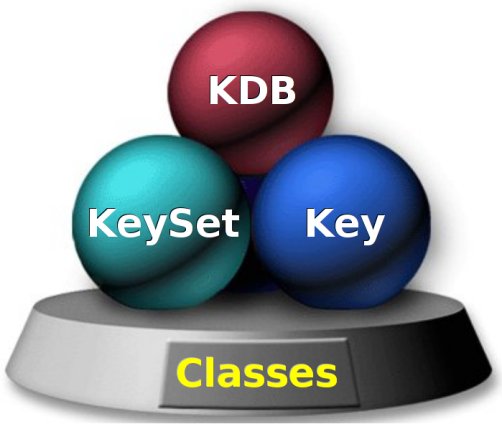
\includegraphics[height=\baselineskip,keepaspectratio=true]{classes.png}%Elektra Classes
\end{DoxyInlineImage}


Some general things you can do with each class are\+:

\mbox{\hyperlink{group__kdb}{KDB (Key Database)}}


\begin{DoxyItemize}
\item \mbox{\hyperlink{group__kdb_ga844e1299a84c3fbf1d3a905c5c893ba5}{Open}} and \mbox{\hyperlink{group__kdb_gadb54dc9fda17ee07deb9444df745c96f}{Close}} the Key Database
\item \mbox{\hyperlink{group__kdb_ga28e385fd9cb7ccfe0b2f1ed2f62453a1}{Get}} and \mbox{\hyperlink{group__kdb_ga11436b058408f83d303ca5e996832bcf}{Set}} \mbox{\hyperlink{group__keyset}{Key\+Set}} in the Key Database
\item See \mbox{\hyperlink{group__kdb}{class documentation}} for more
\end{DoxyItemize}

\mbox{\hyperlink{group__key}{Key}}


\begin{DoxyItemize}
\item \mbox{\hyperlink{group__key_gad23c65b44bf48d773759e1f9a4d43b89}{Create}} and \mbox{\hyperlink{group__key_ga3df95bbc2494e3e6703ece5639be5bb1}{Delete}}
\item Get and Set key the \mbox{\hyperlink{group__keyname_ga7699091610e7f3f43d2949514a4b35d9}{name}}
\item Get and Set \mbox{\hyperlink{group__keyvalue_ga622bde1eb0e0c4994728331326340ef2}{string}} or \mbox{\hyperlink{group__keyvalue_gaa50a5358fd328d373a45f395fa1b99e7}{binary}} values
\item Get and Set \mbox{\hyperlink{group__keymeta}{Metadata}}
\item See \mbox{\hyperlink{group__key}{class documentation}} for more
\end{DoxyItemize}

\mbox{\hyperlink{group__keyset}{Key\+Set}}


\begin{DoxyItemize}
\item \mbox{\hyperlink{group__keyset_ga671e1aaee3ae9dc13b4834a4ddbd2c3c}{Create}} and \mbox{\hyperlink{group__keyset_ga27e5c16473b02a422238c8d970db7ac8}{Delete}}
\item Append \mbox{\hyperlink{group__keyset_gaa5a1d467a4d71041edce68ea7748ce45}{a single key}} or an entire \mbox{\hyperlink{group__keyset_ga21eb9c3a14a604ee3a8bdc779232e7b7}{Key\+Set}}
\item \mbox{\hyperlink{group__keyset_ga60f1ddcf23272f2b29b90e92ebe9b56f}{Lookup keys}}
\item Pop \mbox{\hyperlink{group__keyset_gae42530b04defb772059de0600159cf69}{the last key}}, \mbox{\hyperlink{group__keyset_ga60f1ddcf23272f2b29b90e92ebe9b56f}{a key by name}}, or \mbox{\hyperlink{group__keyset_gaba1f1dbea191f4d7e7eb3e4296ae7d5e}{every key}}
\item Get a key at a \mbox{\hyperlink{group__keyset_gab3fb5e067c672d9fd60a4022b2ae9dd1}{specific position}}
\item Get the \mbox{\hyperlink{group__keyset_ga7474ad6b0a0fa969dbdf267ba5770eee}{number of elements}} in a Key\+Set
\item See \mbox{\hyperlink{group__keyset}{class documentation}} for more
\end{DoxyItemize}

\mbox{\hyperlink{doc_dev_classes_md}{More background information about the classes}}\hypertarget{index_autotoc_md685}{}\doxysection{Namespaces}\label{index_autotoc_md685}
There are 5 trees (=namespaces) of keys\+: {\ttfamily spec}, {\ttfamily proc}, {\ttfamily dir}, {\ttfamily user} and {\ttfamily system} that are all unified (in the given order) in one cascading tree starting with {\ttfamily /}.

The cascading tree is the logical tree to be used in applications. The other trees are the physical ones that stem from configuration sources. When using cascading key the best key will be searched at run-\/time, which appears like a tree on its own. See cascading in the documentation of \mbox{\hyperlink{group__keyset_gad65d2cdcbb5381194a1688e169af8a83}{ks\+Lookup\+By\+Name()}} on how the selection of keys works.


\begin{DoxyItemize}
\item The {\ttfamily spec} tree

This tree specifies how the lookup should take place and also allows us to define defaults or document a key. The metadata of a key contains this information\+:
\begin{DoxyItemize}
\item {\ttfamily override/\#}\+: use these keys {\itshape in favor} of the key itself (note that {\ttfamily \#} is the syntax for arrays, e.\+g. {\ttfamily \#0} for the first element, {\ttfamily \#10} for the 11th and so on)
\item {\ttfamily namespace/\#}\+: instead of using all namespaces in the predefined order, one can specify which namespaces should be searched in which order
\item {\ttfamily fallback/\#}\+: when no key was found in any of the (specified) namespaces the {\ttfamily fallback}-\/keys will be searched
\item {\ttfamily default}\+: this value will be used if nothing else was found
\end{DoxyItemize}
\item The {\ttfamily proc} tree

Is the only read-\/only tree. The configuration does not stem from the \mbox{\hyperlink{group__kdb}{KDB (Key Database)}}, but any other source, e.\+g. command-\/line arguments or environment.
\item The {\ttfamily dir} tree

Allows us to have a per-\/directory overwrite of configuration files, e.\+g. for project specific settings.
\item The {\ttfamily user} tree

Used to store user-\/specific configurations, like the personal settings of a user to certain programs. The user subtree will always be favored if present (except for security concerns the user subtree may not be considered).
\item The {\ttfamily system} tree

It is provided to store system-\/wide configuration keys, that is, the last fallback for applications but the only resort for daemons and system services.
\end{DoxyItemize}

Read more about \mbox{\hyperlink{doc_help_elektra-namespaces_md}{namespaces}} and a tutorial for \mbox{\hyperlink{doc_tutorials_namespaces_md}{namespaces}}.\hypertarget{index_autotoc_md686}{}\doxysection{Rules for Key Names}\label{index_autotoc_md686}
When using Elektra to store your application\textquotesingle{}s configuration and state, please keep in mind the following rules\+:


\begin{DoxyItemize}
\item You are not allowed to create keys right under the root. They are reserved for more generic purposes.
\item The keys for your application, called say {\itshape myapp}, should be created under {\ttfamily /sw/org/myapp/\#0/current}
\begin{DoxyItemize}
\item sw is for software
\item org is the organization. For uniqueness a full reverse url encoded with \textquotesingle{}/\textquotesingle{} instead of \textquotesingle{}.\textquotesingle{} is useful.
\item {\ttfamily \#0} is the major version of the configuration
\item current is the default configuration profile.
\item That means you just need to \mbox{\hyperlink{group__kdb_ga28e385fd9cb7ccfe0b2f1ed2f62453a1}{kdb\+Get()}} {\ttfamily /sw/org/myapp/\#0/profile} and then \mbox{\hyperlink{group__keyset_gad65d2cdcbb5381194a1688e169af8a83}{ks\+Lookup\+By\+Name()}} in {\ttfamily /sw/org/myapp/\#0/profile/key} where profile is from command-\/line arguments and defaults to current.
\end{DoxyItemize}
\end{DoxyItemize}

Read more about \mbox{\hyperlink{doc_help_elektra-key-names_md}{key names}}\hypertarget{index_autotoc_md687}{}\doxysection{Backend Overview}\label{index_autotoc_md687}
The core of Elektra does not store configuration itself to the hard disk. Instead this work is delegated to backends.

If you want to develop a backend, you should already have some experience with Elektra from the user point of view. You should be familiar with the data structures\+: \mbox{\hyperlink{group__key}{Key}} and \mbox{\hyperlink{group__keyset}{Key\+Set}} Then you can start reading about Backends that are composed out of \mbox{\hyperlink{group__plugin}{Plugins}}. To get started with writing plugins, first read our \mbox{\hyperlink{doc_tutorials_plugins_md}{plugin tutorial}} and then lookup details in the API description in \mbox{\hyperlink{group__plugin}{Plugins}}.

Read more about \mbox{\hyperlink{doc_help_elektra-mounting_md}{mounting}}\hypertarget{index_autotoc_md688}{}\doxysection{See Also}\label{index_autotoc_md688}

\begin{DoxyItemize}
\item See \mbox{\hyperlink{doc_help_elektra-glossary_md}{elektra-\/glossary(7)}}
\item More information about \mbox{\hyperlink{doc_help_elektra-backends_md}{elektra-\/backends(7)}}
\item More information about \mbox{\hyperlink{doc_dev_plugins-framework_md}{plugins-\/framework}} 
\end{DoxyItemize}
\chapter{Deprecated List}
\label{deprecated}
\hypertarget{deprecated}{}

\begin{DoxyRefList}
\item[\label{deprecated__deprecated000005}%
\Hypertarget{deprecated__deprecated000005}%
Member \hyperlink{group__invoke_gaae89e2497eba478be2043f1b25adbb3c}{elektra\+Invoke\+Initialize} (const char $\ast$elektra\+Plugin\+Name)]Do not use. 
\item[\label{deprecated__deprecated000007}%
\Hypertarget{deprecated__deprecated000007}%
Member \hyperlink{classkdb_1_1tools_1_1Modules_a6ae72cc8e30fe3fb0aabd6f78fad8ddf}{kdb\+:\+:tools\+:\+:Modules\+:\+:load} (std\+::string const \&plugin\+Name, \hyperlink{classkdb_1_1KeySet}{kdb\+::\+Key\+Set} const \&config)]do not use  
\item[\label{deprecated__deprecated000006}%
\Hypertarget{deprecated__deprecated000006}%
Member \hyperlink{classkdb_1_1tools_1_1Modules_ae8d8c91745c9f517e6e8a556f1664f69}{kdb\+:\+:tools\+:\+:Modules\+:\+:load} (std\+::string const \&plugin\+Name)]do not use  
\item[\label{deprecated__deprecated000001}%
\Hypertarget{deprecated__deprecated000001}%
Member \hyperlink{group__key_gga9b703ca49f48b482def322b77d3e6bc8ab089c5e7977d6e58737eb586ee153b7f}{K\+E\+Y\+\_\+\+N\+U\+LL} ]do not use  
\item[\label{deprecated__deprecated000004}%
\Hypertarget{deprecated__deprecated000004}%
Member \hyperlink{group__keytest_gaf247df0de7aca04b32ef80e39ef12950}{key\+Need\+Sync} (const \hyperlink{classkdb_1_1Key}{Key} $\ast$key)]The handling of synchronization is done internally and does not need to be checked by neither application nor plugins. 
\item[\label{deprecated__deprecated000002}%
\Hypertarget{deprecated__deprecated000002}%
Member \hyperlink{group__key_gad23c65b44bf48d773759e1f9a4d43b89}{key\+New} (const char $\ast$name,...)]The flags below are deprecated and \hyperlink{group__key_gga9b703ca49f48b482def322b77d3e6bc8a040582834bb2d90049947d7ef74e87e2}{K\+E\+Y\+\_\+\+M\+E\+TA} should be preferred. They remain some time, however, for compatibility\+: 
\begin{DoxyCodeInclude}
\end{DoxyCodeInclude}

\begin{DoxyItemize}
\item \hyperlink{group__key_gga9b703ca49f48b482def322b77d3e6bc8ac29427bb47cc31689d02912e36161ee3}{K\+E\+Y\+\_\+\+C\+O\+M\+M\+E\+NT} ~\newline
 Next parameter is a comment. See \hyperlink{group__meta_ga8863a877a84fa46e6017fe72e49b89c1}{key\+Set\+Comment()}. 
\begin{DoxyCodeInclude}
\end{DoxyCodeInclude}
Member \hyperlink{group__keyset_ga8f210432e664d8ba06d7d55a2aba2d0f}{ks\+Need\+Sync} (const \hyperlink{classkdb_1_1KeySet}{Key\+Set} $\ast$ks) \hyperlink{classkdb_1_1tools_1_1Backends}{Backends} now work differently and do not rely on this information.
\end{DoxyItemize}
\end{DoxyRefList}
\chapter{Module Index}
\section{Modules}
Here is a list of all modules\+:\begin{DoxyCompactList}
\item \contentsline{section}{K\+D\+B}{\pageref{group__kdb}}{}
\item \contentsline{section}{Key}{\pageref{group__key}}{}
\begin{DoxyCompactList}
\item \contentsline{section}{Meta Info Manipulation Methods}{\pageref{group__keymeta}}{}
\item \contentsline{section}{Methods for Making Tests}{\pageref{group__keytest}}{}
\item \contentsline{section}{Name Manipulation Methods}{\pageref{group__keyname}}{}
\item \contentsline{section}{Value Manipulation Methods}{\pageref{group__keyvalue}}{}
\end{DoxyCompactList}
\item \contentsline{section}{Key\+Set}{\pageref{group__keyset}}{}
\item \contentsline{section}{Plugins}{\pageref{group__plugin}}{}
\item \contentsline{section}{Proposals for Elektra}{\pageref{group__proposal}}{}
\begin{DoxyCompactList}
\item \contentsline{section}{A\+P\+I Proposals for Elektra}{\pageref{group__api}}{}
\item \contentsline{section}{Meta Data proposal+compatibility}{\pageref{group__meta}}{}
\end{DoxyCompactList}
\end{DoxyCompactList}

\chapter{Namespace Index}
\section{Namespace List}
Here is a list of all documented namespaces with brief descriptions\-:\begin{DoxyCompactList}
\item\contentsline{section}{\hyperlink{namespacekdb}{kdb} \\*This is the main namespace for the C++ binding and libraries }{\pageref{namespacekdb}}{}
\item\contentsline{section}{\hyperlink{namespacekdb_1_1tools}{kdb\-::tools} \\*This namespace is for the libtool library }{\pageref{namespacekdb_1_1tools}}{}
\end{DoxyCompactList}

\chapter{Data Structure Index}
\section{Class Hierarchy}
This inheritance list is sorted roughly, but not completely, alphabetically\-:\begin{DoxyCompactList}
\item \contentsline{section}{kdb\-:\-:tools\-:\-:Backend}{\pageref{classkdb_1_1tools_1_1Backend}}{}
\item \contentsline{section}{kdb\-:\-:tools\-:\-:Backend\-Info}{\pageref{structkdb_1_1tools_1_1BackendInfo}}{}
\item \contentsline{section}{kdb\-:\-:tools\-:\-:Backends}{\pageref{classkdb_1_1tools_1_1Backends}}{}
\item \contentsline{section}{kdb\-:\-:Context}{\pageref{classkdb_1_1Context}}{}
\item \contentsline{section}{kdb\-:\-:Default\-Get\-Policy$<$ T $>$}{\pageref{classkdb_1_1DefaultGetPolicy}}{}
\item \contentsline{section}{kdb\-:\-:Default\-Set\-Policy}{\pageref{classkdb_1_1DefaultSetPolicy}}{}
\item \contentsline{section}{kdb\-:\-:Discriminator$<$ Base, D $>$}{\pageref{classkdb_1_1Discriminator}}{}
\item \contentsline{section}{kdb\-:\-:Discriminator$<$ Setter1, 1 $>$}{\pageref{classkdb_1_1Discriminator}}{}
\item \contentsline{section}{kdb\-:\-:Discriminator$<$ Setter2, 2 $>$}{\pageref{classkdb_1_1Discriminator}}{}
\item std\-:\-:exception\begin{DoxyCompactList}
\item std\-:\-:runtime\-\_\-error\begin{DoxyCompactList}
\item \contentsline{section}{kdb\-:\-:tools\-:\-:Tool\-Exception}{\pageref{structkdb_1_1tools_1_1ToolException}}{}
\end{DoxyCompactList}
\end{DoxyCompactList}
\item \contentsline{section}{kdb\-:\-:Get\-Policy\-Is$<$ Policy $>$}{\pageref{classkdb_1_1GetPolicyIs}}{}
\item \contentsline{section}{kdb\-:\-:K\-D\-B}{\pageref{classkdb_1_1KDB}}{}
\item \contentsline{section}{kdb\-:\-:Key}{\pageref{classkdb_1_1Key}}{}
\item \contentsline{section}{kdb\-:\-:Key\-Set}{\pageref{classkdb_1_1KeySet}}{}
\item \contentsline{section}{kdb\-:\-:Key\-Set\-Iterator}{\pageref{classkdb_1_1KeySetIterator}}{}
\item \contentsline{section}{kdb\-:\-:Key\-Set\-Reverse\-Iterator}{\pageref{classkdb_1_1KeySetReverseIterator}}{}
\item \contentsline{section}{kdb\-:\-:tools\-:\-:Modules}{\pageref{classkdb_1_1tools_1_1Modules}}{}
\item \contentsline{section}{kdb\-:\-:tools\-:\-:Plugin}{\pageref{classkdb_1_1tools_1_1Plugin}}{}
\item \contentsline{section}{kdb\-:\-:tools\-:\-:Plugins}{\pageref{classkdb_1_1tools_1_1Plugins}}{}
\item \contentsline{section}{kdb\-:\-:Set\-Policy\-Is$<$ Policy $>$}{\pageref{classkdb_1_1SetPolicyIs}}{}
\end{DoxyCompactList}

\chapter{Data Structure Index}
\section{Data Structures}
Here are the data structures with brief descriptions:\begin{DoxyCompactList}
\item\contentsline{section}{\hyperlink{struct__Backend}{\_\-Backend} }{\pageref{struct__Backend}}{}
\item\contentsline{section}{\hyperlink{struct__KDB}{\_\-KDB} }{\pageref{struct__KDB}}{}
\item\contentsline{section}{\hyperlink{struct__Key}{\_\-Key} }{\pageref{struct__Key}}{}
\item\contentsline{section}{\hyperlink{struct__KeySet}{\_\-KeySet} }{\pageref{struct__KeySet}}{}
\item\contentsline{section}{\hyperlink{struct__Plugin}{\_\-Plugin} }{\pageref{struct__Plugin}}{}
\item\contentsline{section}{\hyperlink{struct__Split}{\_\-Split} }{\pageref{struct__Split}}{}
\item\contentsline{section}{\hyperlink{struct__Trie}{\_\-Trie} }{\pageref{struct__Trie}}{}
\item\contentsline{section}{\hyperlink{classflat__copy}{flat\_\-copy} }{\pageref{classflat__copy}}{}
\end{DoxyCompactList}

\chapter{File Index}
\section{File List}
Here is a list of all documented files with brief descriptions\+:\begin{DoxyCompactList}
\item\contentsline{section}{\hyperlink{array_8c}{array.\+c} \\*Array methods }{\pageref{array_8c}}{}
\item\contentsline{section}{\hyperlink{automergeconfiguration_8cpp}{automergeconfiguration.\+cpp} }{\pageref{automergeconfiguration_8cpp}}{}
\item\contentsline{section}{\hyperlink{automergeconfiguration_8hpp}{automergeconfiguration.\+hpp} \\*A configuration for a simple automerge }{\pageref{automergeconfiguration_8hpp}}{}
\item\contentsline{section}{\hyperlink{automergestrategy_8cpp}{automergestrategy.\+cpp} \\*Implementation of Auto\+Merge\+Strategy }{\pageref{automergestrategy_8cpp}}{}
\item\contentsline{section}{\hyperlink{automergestrategy_8hpp}{automergestrategy.\+hpp} \\*A strategy for taking the value of }{\pageref{automergestrategy_8hpp}}{}
\item\contentsline{section}{\hyperlink{backend_8c}{backend.\+c} \\*Everything related to a backend }{\pageref{backend_8c}}{}
\item\contentsline{section}{\hyperlink{examples_2backend_8cpp}{examples/backend.\+cpp} }{\pageref{examples_2backend_8cpp}}{}
\item\contentsline{section}{\hyperlink{src_2backend_8cpp}{src/backend.\+cpp} \\*Implementation of backend }{\pageref{src_2backend_8cpp}}{}
\item\contentsline{section}{\hyperlink{backend_8hpp}{backend.\+hpp} \\*Implements a way to deal with a backend }{\pageref{backend_8hpp}}{}
\item\contentsline{section}{\hyperlink{backendbuilder_8cpp}{backendbuilder.\+cpp} \\*Implementation of backend builder }{\pageref{backendbuilder_8cpp}}{}
\item\contentsline{section}{\hyperlink{backendbuilder_8hpp}{backendbuilder.\+hpp} \\*Implements a way to build backends }{\pageref{backendbuilder_8hpp}}{}
\item\contentsline{section}{\hyperlink{backendparser_8cpp}{backendparser.\+cpp} \\*Tests for the Backend parser class }{\pageref{backendparser_8cpp}}{}
\item\contentsline{section}{\hyperlink{backendparser_8hpp}{backendparser.\+hpp} \\*Implements ways to parse backends }{\pageref{backendparser_8hpp}}{}
\item\contentsline{section}{\hyperlink{backends_8cpp}{backends.\+cpp} }{\pageref{backends_8cpp}}{}
\item\contentsline{section}{\hyperlink{backends_8hpp}{backends.\+hpp} \\*Allows one to list all available backends }{\pageref{backends_8hpp}}{}
\item\contentsline{section}{\hyperlink{benchmark__crypto__comparison_8cpp}{benchmark\+\_\+crypto\+\_\+comparison.\+cpp} \\*Benchmark for comparing the cryptographic providers used in the crypto plugin }{\pageref{benchmark__crypto__comparison_8cpp}}{}
\item\contentsline{section}{\hyperlink{benchmark__plugins_8cpp}{benchmark\+\_\+plugins.\+cpp} \\*Benchmark for getenv }{\pageref{benchmark__plugins_8cpp}}{}
\item\contentsline{section}{\hyperlink{comparison_8cpp}{comparison.\+cpp} \\*Comparison helper functions }{\pageref{comparison_8cpp}}{}
\item\contentsline{section}{\hyperlink{comparison_8hpp}{comparison.\+hpp} \\*Comparison helper functions }{\pageref{comparison_8hpp}}{}
\item\contentsline{section}{\hyperlink{conversion_8h}{conversion.\+h} \\*Elektra conversion }{\pageref{conversion_8h}}{}
\item\contentsline{section}{\hyperlink{dbus_8c}{dbus.\+c} \\*I/O Adapter for D-\/\+Bus }{\pageref{dbus_8c}}{}
\item\contentsline{section}{\hyperlink{dbus_8h}{dbus.\+h} \\*I/O Adapter for D-\/\+Bus }{\pageref{dbus_8h}}{}
\item\contentsline{section}{\hyperlink{dl_8c}{dl.\+c} \\*Loading modules under linux }{\pageref{dl_8c}}{}
\item\contentsline{section}{\hyperlink{doc_8c}{doc.\+c} \\*Loading Modules for Elektra documentation }{\pageref{doc_8c}}{}
\item\contentsline{section}{\hyperlink{doc_8h}{doc.\+h} }{\pageref{doc_8h}}{}
\item\contentsline{section}{\hyperlink{elektra_8c}{elektra.\+c} \\*Elektra High Level A\+PI }{\pageref{elektra_8c}}{}
\item\contentsline{section}{\hyperlink{elektra_8h}{elektra.\+h} \\*Elektra High Level A\+PI }{\pageref{elektra_8h}}{}
\item\contentsline{section}{\hyperlink{elektra__array__value_8c}{elektra\+\_\+array\+\_\+value.\+c} \\*Elektra High Level A\+PI }{\pageref{elektra__array__value_8c}}{}
\item\contentsline{section}{\hyperlink{elektra__conversion_8c}{elektra\+\_\+conversion.\+c} \\*Elektra High Level A\+PI }{\pageref{elektra__conversion_8c}}{}
\item\contentsline{section}{\hyperlink{elektra__error_8c}{elektra\+\_\+error.\+c} \\*Elektra error codes }{\pageref{elektra__error_8c}}{}
\item\contentsline{section}{\hyperlink{elektra__value_8c}{elektra\+\_\+value.\+c} \\*Elektra High Level A\+PI }{\pageref{elektra__value_8c}}{}
\item\contentsline{section}{\hyperlink{error_8h}{error.\+h} \\*Elektra error }{\pageref{error_8h}}{}
\item\contentsline{section}{\hyperlink{ev_8h}{ev.\+h} \\*Declarations for the ev I/O binding }{\pageref{ev_8h}}{}
\item\contentsline{section}{\hyperlink{functional_8c}{functional.\+c} \\*Functional helper }{\pageref{functional_8c}}{}
\item\contentsline{section}{\hyperlink{glib_8h}{glib.\+h} \\*Declarations for the glib I/O binding }{\pageref{glib_8h}}{}
\item\contentsline{section}{\hyperlink{global_8c}{global.\+c} \\*Helpers for global plugins }{\pageref{global_8c}}{}
\item\contentsline{section}{\hyperlink{globbing_8c}{globbing.\+c} \\*Library for performing globbing on keynames }{\pageref{globbing_8c}}{}
\item\contentsline{section}{\hyperlink{importmergeconfiguration_8cpp}{importmergeconfiguration.\+cpp} }{\pageref{importmergeconfiguration_8cpp}}{}
\item\contentsline{section}{\hyperlink{importmergeconfiguration_8hpp}{importmergeconfiguration.\+hpp} \\*A configuration for a simple automerge and guaranteed conflict resolution by one side }{\pageref{importmergeconfiguration_8hpp}}{}
\item\contentsline{section}{\hyperlink{interactivemergestrategy_8cpp}{interactivemergestrategy.\+cpp} \\*Implementation of Interactive\+Merge\+Strategy }{\pageref{interactivemergestrategy_8cpp}}{}
\item\contentsline{section}{\hyperlink{interactivemergestrategy_8hpp}{interactivemergestrategy.\+hpp} \\*Interactive merge strategy asking for user input at each step }{\pageref{interactivemergestrategy_8hpp}}{}
\item\contentsline{section}{\hyperlink{internal_8c}{internal.\+c} \\*Internal methods for Elektra }{\pageref{internal_8c}}{}
\item\contentsline{section}{\hyperlink{invoke_8c}{invoke.\+c} \\*Library for invoking exported plugin functions }{\pageref{invoke_8c}}{}
\item\contentsline{section}{\hyperlink{io_8c}{io.\+c} \\*Implementation of I/O functions as defined in \hyperlink{kdbio_8h}{kdbio.\+h} }{\pageref{io_8c}}{}
\item\contentsline{section}{\hyperlink{io__doc_8c}{io\+\_\+doc.\+c} \\*I/O example binding }{\pageref{io__doc_8c}}{}
\item\contentsline{section}{\hyperlink{kdb_8c}{kdb.\+c} \\*Low level functions for access the Key Database }{\pageref{kdb_8c}}{}
\item\contentsline{section}{\hyperlink{kdb_8hpp}{kdb.\+hpp} }{\pageref{kdb_8hpp}}{}
\item\contentsline{section}{\hyperlink{kdbassert_8h}{kdbassert.\+h} \\*Assertions macros }{\pageref{kdbassert_8h}}{}
\item\contentsline{section}{\hyperlink{kdbcontext_8hpp}{kdbcontext.\+hpp} }{\pageref{kdbcontext_8hpp}}{}
\item\contentsline{section}{\hyperlink{kdbenum_8c}{kdbenum.\+c} \\*Dummy file do document the enums which have no name in the header file }{\pageref{kdbenum_8c}}{}
\item\contentsline{section}{\hyperlink{kdbexcept_8hpp}{kdbexcept.\+hpp} }{\pageref{kdbexcept_8hpp}}{}
\item\contentsline{section}{\hyperlink{kdbextension_8h}{kdbextension.\+h} \\*Extension functionality }{\pageref{kdbextension_8h}}{}
\item\contentsline{section}{\hyperlink{kdbglobal_8h}{kdbglobal.\+h} \\*Defines for global plugins }{\pageref{kdbglobal_8h}}{}
\item\contentsline{section}{\hyperlink{kdbhelper_8h}{kdbhelper.\+h} \\*Helper for memory management }{\pageref{kdbhelper_8h}}{}
\item\contentsline{section}{\hyperlink{kdbinternal_8h}{kdbinternal.\+h} \\*Includes most internal header files }{\pageref{kdbinternal_8h}}{}
\item\contentsline{section}{\hyperlink{kdbio_8h}{kdbio.\+h} \\*Elektra-\/\+I/O structures for I/O bindings, plugins and applications }{\pageref{kdbio_8h}}{}
\item\contentsline{section}{\hyperlink{kdbio_8hpp}{kdbio.\+hpp} }{\pageref{kdbio_8hpp}}{}
\item\contentsline{section}{\hyperlink{kdbio__doc_8h}{kdbio\+\_\+doc.\+h} \\*Declarations for the doc I/O binding }{\pageref{kdbio__doc_8h}}{}
\item\contentsline{section}{\hyperlink{kdbioplugin_8h}{kdbioplugin.\+h} \\*Elektra-\/\+I/O functions and declarations for the I/O binding test suite }{\pageref{kdbioplugin_8h}}{}
\item\contentsline{section}{\hyperlink{kdbioprivate_8h}{kdbioprivate.\+h} \\*Private Elektra-\/\+IO structures for I/O bindings, plugins and applications }{\pageref{kdbioprivate_8h}}{}
\item\contentsline{section}{\hyperlink{kdbiotest_8h}{kdbiotest.\+h} \\*Elektra-\/\+I/O functions and declarations for the I/O binding test suite }{\pageref{kdbiotest_8h}}{}
\item\contentsline{section}{\hyperlink{kdblogger_8h}{kdblogger.\+h} \\*Logger Interface }{\pageref{kdblogger_8h}}{}
\item\contentsline{section}{\hyperlink{kdbmacros_8h}{kdbmacros.\+h} \\*Macros by Elektra }{\pageref{kdbmacros_8h}}{}
\item\contentsline{section}{\hyperlink{kdbmeta_8h}{kdbmeta.\+h} \\*Metadata functions }{\pageref{kdbmeta_8h}}{}
\item\contentsline{section}{\hyperlink{kdbmodule_8h}{kdbmodule.\+h} }{\pageref{kdbmodule_8h}}{}
\item\contentsline{section}{\hyperlink{kdbnotification_8h}{kdbnotification.\+h} \\*Elektra-\/\+Notification structures and declarations for application developers }{\pageref{kdbnotification_8h}}{}
\item\contentsline{section}{\hyperlink{kdbnotificationinternal_8h}{kdbnotificationinternal.\+h} \\*Elektra-\/\+Notification structures and declarations for developing notification and transport plugins }{\pageref{kdbnotificationinternal_8h}}{}
\item\contentsline{section}{\hyperlink{kdbobsolete_8h}{kdbobsolete.\+h} \\*Obsolete/\+Deprecated A\+PI }{\pageref{kdbobsolete_8h}}{}
\item\contentsline{section}{\hyperlink{kdbopmphm_8h}{kdbopmphm.\+h} \\*Defines for the Order Preserving Minimal Perfect Hash Map }{\pageref{kdbopmphm_8h}}{}
\item\contentsline{section}{\hyperlink{kdbopmphmpredictor_8h}{kdbopmphmpredictor.\+h} \\*Defines for the Order Preserving Minimal Perfect Hash Map Predictor }{\pageref{kdbopmphmpredictor_8h}}{}
\item\contentsline{section}{\hyperlink{kdbopts_8h}{kdbopts.\+h} }{\pageref{kdbopts_8h}}{}
\item\contentsline{section}{\hyperlink{kdbos_8h}{kdbos.\+h} \\*Operating system specific workarounds }{\pageref{kdbos_8h}}{}
\item\contentsline{section}{\hyperlink{kdbplugin_8h}{kdbplugin.\+h} \\*Methods for plugin programing }{\pageref{kdbplugin_8h}}{}
\item\contentsline{section}{\hyperlink{kdbplugin_8hpp}{kdbplugin.\+hpp} \\*Helpers for creating plugins }{\pageref{kdbplugin_8hpp}}{}
\item\contentsline{section}{\hyperlink{kdbprivate_8h}{kdbprivate.\+h} \\*Private declarations }{\pageref{kdbprivate_8h}}{}
\item\contentsline{section}{\hyperlink{kdbproposal_8h}{kdbproposal.\+h} \\*Proposed declarations }{\pageref{kdbproposal_8h}}{}
\item\contentsline{section}{\hyperlink{kdbrand_8h}{kdbrand.\+h} \\*Defines for Rand }{\pageref{kdbrand_8h}}{}
\item\contentsline{section}{\hyperlink{kdbthread_8hpp}{kdbthread.\+hpp} }{\pageref{kdbthread_8hpp}}{}
\item\contentsline{section}{\hyperlink{kdbtimer_8hpp}{kdbtimer.\+hpp} }{\pageref{kdbtimer_8hpp}}{}
\item\contentsline{section}{\hyperlink{kdbtypes_8h}{kdbtypes.\+h} \\*Elektra’s data types for C and C++11 }{\pageref{kdbtypes_8h}}{}
\item\contentsline{section}{\hyperlink{kdbvalue_8hpp}{kdbvalue.\+hpp} }{\pageref{kdbvalue_8hpp}}{}
\item\contentsline{section}{\hyperlink{key_8c}{key.\+c} \\*Methods for Key manipulation }{\pageref{key_8c}}{}
\item\contentsline{section}{\hyperlink{key_8hpp}{key.\+hpp} }{\pageref{key_8hpp}}{}
\item\contentsline{section}{\hyperlink{keyexcept_8hpp}{keyexcept.\+hpp} }{\pageref{keyexcept_8hpp}}{}
\item\contentsline{section}{\hyperlink{keyhelper_8cpp}{keyhelper.\+cpp} \\*Key helper functions }{\pageref{keyhelper_8cpp}}{}
\item\contentsline{section}{\hyperlink{keyhelper_8hpp}{keyhelper.\+hpp} \\*Key helper functions }{\pageref{keyhelper_8hpp}}{}
\item\contentsline{section}{\hyperlink{keyhelpers_8c}{keyhelpers.\+c} \\*Helpers for key manipulation }{\pageref{keyhelpers_8c}}{}
\item\contentsline{section}{\hyperlink{keyio_8hpp}{keyio.\+hpp} }{\pageref{keyio_8hpp}}{}
\item\contentsline{section}{\hyperlink{keymeta_8c}{keymeta.\+c} \\*Methods to do various operations on Key metadata }{\pageref{keymeta_8c}}{}
\item\contentsline{section}{\hyperlink{ease_2keyname_8c}{ease/keyname.\+c} \\*Methods for accessing key names }{\pageref{ease_2keyname_8c}}{}
\item\contentsline{section}{\hyperlink{elektra_2keyname_8c}{elektra/keyname.\+c} \\*Methods for Key name manipulation }{\pageref{elektra_2keyname_8c}}{}
\item\contentsline{section}{\hyperlink{keyset_8c}{keyset.\+c} \\*Methods for key sets }{\pageref{keyset_8c}}{}
\item\contentsline{section}{\hyperlink{keyset_8hpp}{keyset.\+hpp} }{\pageref{keyset_8hpp}}{}
\item\contentsline{section}{\hyperlink{keysetget_8hpp}{keysetget.\+hpp} }{\pageref{keysetget_8hpp}}{}
\item\contentsline{section}{\hyperlink{keysetio_8hpp}{keysetio.\+hpp} }{\pageref{keysetio_8hpp}}{}
\item\contentsline{section}{\hyperlink{keytest_8c}{keytest.\+c} \\*Methods for making tests }{\pageref{keytest_8c}}{}
\item\contentsline{section}{\hyperlink{keyvalue_8c}{keyvalue.\+c} \\*Methods for Key value manipulation }{\pageref{keyvalue_8c}}{}
\item\contentsline{section}{\hyperlink{log_8c}{log.\+c} \\*Non-\/\+C99 Logger Implementation }{\pageref{log_8c}}{}
\item\contentsline{section}{\hyperlink{markdownlinkconverter_8c}{markdownlinkconverter.\+c} }{\pageref{markdownlinkconverter_8c}}{}
\item\contentsline{section}{\hyperlink{mergeconfiguration_8hpp}{mergeconfiguration.\+hpp} \\*Base class for defining preconfigured merge configurations }{\pageref{mergeconfiguration_8hpp}}{}
\item\contentsline{section}{\hyperlink{mergeconflict_8hpp}{mergeconflict.\+hpp} \\*Models a merge conflict }{\pageref{mergeconflict_8hpp}}{}
\item\contentsline{section}{\hyperlink{mergeconflictstrategy_8cpp}{mergeconflictstrategy.\+cpp} \\*Implementation of Merge\+Conflict\+Strategy }{\pageref{mergeconflictstrategy_8cpp}}{}
\item\contentsline{section}{\hyperlink{mergeconflictstrategy_8hpp}{mergeconflictstrategy.\+hpp} \\*Interface for a Merge\+Conflict\+Strategy }{\pageref{mergeconflictstrategy_8hpp}}{}
\item\contentsline{section}{\hyperlink{mergeresult_8cpp}{mergeresult.\+cpp} \\*Implementation of Merge\+Result }{\pageref{mergeresult_8cpp}}{}
\item\contentsline{section}{\hyperlink{mergeresult_8hpp}{mergeresult.\+hpp} \\*Class modelling the result of a three way merge }{\pageref{mergeresult_8hpp}}{}
\item\contentsline{section}{\hyperlink{mergetask_8hpp}{mergetask.\+hpp} \\*Models a merge task }{\pageref{mergetask_8hpp}}{}
\item\contentsline{section}{\hyperlink{mergetestutils_8cpp}{mergetestutils.\+cpp} \\*Implements a helper class for merge related tests }{\pageref{mergetestutils_8cpp}}{}
\item\contentsline{section}{\hyperlink{merging_8cpp}{merging.\+cpp} }{\pageref{merging_8cpp}}{}
\item\contentsline{section}{\hyperlink{mergingkdb_8cpp}{mergingkdb.\+cpp} \\*Implementation of Merge\+Result }{\pageref{mergingkdb_8cpp}}{}
\item\contentsline{section}{\hyperlink{mergingkdb_8hpp}{mergingkdb.\+hpp} }{\pageref{mergingkdb_8hpp}}{}
\item\contentsline{section}{\hyperlink{meta_8c}{meta.\+c} \\*Methods for metadata manipulation }{\pageref{meta_8c}}{}
\item\contentsline{section}{\hyperlink{metamergestrategy_8cpp}{metamergestrategy.\+cpp} \\*Implementation of Meta\+Merge\+Strategy }{\pageref{metamergestrategy_8cpp}}{}
\item\contentsline{section}{\hyperlink{metamergestrategy_8hpp}{metamergestrategy.\+hpp} \\*Applies a Merge\+Conflict\+Strategy on the metakeys }{\pageref{metamergestrategy_8hpp}}{}
\item\contentsline{section}{\hyperlink{modules_8cpp}{modules.\+cpp} \\*Implementation of module loading }{\pageref{modules_8cpp}}{}
\item\contentsline{section}{\hyperlink{modules_8hpp}{modules.\+hpp} \\*Allows one to load plugins }{\pageref{modules_8hpp}}{}
\item\contentsline{section}{\hyperlink{mount_8c}{mount.\+c} \\*Internals of mount functionality }{\pageref{mount_8c}}{}
\item\contentsline{section}{\hyperlink{newkeystrategy_8cpp}{newkeystrategy.\+cpp} \\*Implementation of One\+Side\+Strategy }{\pageref{newkeystrategy_8cpp}}{}
\item\contentsline{section}{\hyperlink{newkeystrategy_8hpp}{newkeystrategy.\+hpp} \\*A strategy which always takes the value from one side }{\pageref{newkeystrategy_8hpp}}{}
\item\contentsline{section}{\hyperlink{nolog_8c}{nolog.\+c} \\*C99-\/compatible Fake Logger Implementation }{\pageref{nolog_8c}}{}
\item\contentsline{section}{\hyperlink{notification_8c}{notification.\+c} \\*Implementation of notification functions as defined in \hyperlink{kdbnotification_8h}{kdbnotification.\+h} }{\pageref{notification_8c}}{}
\item\contentsline{section}{\hyperlink{onesidemergeconfiguration_8cpp}{onesidemergeconfiguration.\+cpp} }{\pageref{onesidemergeconfiguration_8cpp}}{}
\item\contentsline{section}{\hyperlink{onesidemergeconfiguration_8hpp}{onesidemergeconfiguration.\+hpp} \\*A configuration for a simple automerge and guaranteed conflict resolution by one side }{\pageref{onesidemergeconfiguration_8hpp}}{}
\item\contentsline{section}{\hyperlink{onesidestrategy_8cpp}{onesidestrategy.\+cpp} \\*Implementation of One\+Side\+Strategy }{\pageref{onesidestrategy_8cpp}}{}
\item\contentsline{section}{\hyperlink{onesidestrategy_8hpp}{onesidestrategy.\+hpp} \\*A strategy which always takes the value from one side }{\pageref{onesidestrategy_8hpp}}{}
\item\contentsline{section}{\hyperlink{onesidevaluestrategy_8cpp}{onesidevaluestrategy.\+cpp} \\*Implementation of One\+Side\+Strategy }{\pageref{onesidevaluestrategy_8cpp}}{}
\item\contentsline{section}{\hyperlink{onesidevaluestrategy_8hpp}{onesidevaluestrategy.\+hpp} }{\pageref{onesidevaluestrategy_8hpp}}{}
\item\contentsline{section}{\hyperlink{opmphm_8c}{opmphm.\+c} \\*The Order Preserving Minimal Perfect Hash Map }{\pageref{opmphm_8c}}{}
\item\contentsline{section}{\hyperlink{opmphmpredictor_8c}{opmphmpredictor.\+c} \\*The Order Preserving Minimal Perfect Hash Map Predictor }{\pageref{opmphmpredictor_8c}}{}
\item\contentsline{section}{\hyperlink{opts_8c}{opts.\+c} }{\pageref{opts_8c}}{}
\item\contentsline{section}{\hyperlink{overwritemergeconfiguration_8cpp}{overwritemergeconfiguration.\+cpp} }{\pageref{overwritemergeconfiguration_8cpp}}{}
\item\contentsline{section}{\hyperlink{overwritemergeconfiguration_8hpp}{overwritemergeconfiguration.\+hpp} \\*A configuration for a simple automerge and guaranteed conflict resolution by one side }{\pageref{overwritemergeconfiguration_8hpp}}{}
\item\contentsline{section}{\hyperlink{owner_8c}{owner.\+c} \\*Obsolete owner methods }{\pageref{owner_8c}}{}
\item\contentsline{section}{\hyperlink{elektra_2plugin_8c}{elektra/plugin.\+c} \\*Interna of plugin functionality }{\pageref{elektra_2plugin_8c}}{}
\item\contentsline{section}{\hyperlink{plugin_2plugin_8c}{plugin/plugin.\+c} \\*Access plugin handle }{\pageref{plugin_2plugin_8c}}{}
\item\contentsline{section}{\hyperlink{plugin_8cpp}{plugin.\+cpp} \\*Implementation of plugin }{\pageref{plugin_8cpp}}{}
\item\contentsline{section}{\hyperlink{plugin_8hpp}{plugin.\+hpp} \\*Header file of plugin }{\pageref{plugin_8hpp}}{}
\item\contentsline{section}{\hyperlink{plugindatabase_8cpp}{plugindatabase.\+cpp} \\*Implementation of Plugin\+Database(s) }{\pageref{plugindatabase_8cpp}}{}
\item\contentsline{section}{\hyperlink{plugindatabase_8hpp}{plugindatabase.\+hpp} \\*Interface to all plugins }{\pageref{plugindatabase_8hpp}}{}
\item\contentsline{section}{\hyperlink{pluginprocess_8c}{pluginprocess.\+c} \\*Source for the pluginprocess library }{\pageref{pluginprocess_8c}}{}
\item\contentsline{section}{\hyperlink{plugins_8cpp}{plugins.\+cpp} \\*Implementation of set/get/error plugins }{\pageref{plugins_8cpp}}{}
\item\contentsline{section}{\hyperlink{plugins_8hpp}{plugins.\+hpp} \\*Implementation of get/set and error plugins }{\pageref{plugins_8hpp}}{}
\item\contentsline{section}{\hyperlink{pluginspec_8cpp}{pluginspec.\+cpp} \\*Implementation of plugin spec }{\pageref{pluginspec_8cpp}}{}
\item\contentsline{section}{\hyperlink{pluginspec_8hpp}{pluginspec.\+hpp} \\*Interface to specify which plugin is meant }{\pageref{pluginspec_8hpp}}{}
\item\contentsline{section}{\hyperlink{elektra_2proposal_8c}{elektra/proposal.\+c} \\*Implementation of proposed A\+PI enhancements }{\pageref{elektra_2proposal_8c}}{}
\item\contentsline{section}{\hyperlink{proposal_2proposal_8c}{proposal/proposal.\+c} \\*Implementation of proposed A\+PI enhancements }{\pageref{proposal_2proposal_8c}}{}
\item\contentsline{section}{\hyperlink{rand_8c}{rand.\+c} \\*Rand for Elektra }{\pageref{rand_8c}}{}
\item\contentsline{section}{\hyperlink{reference_8c}{reference.\+c} \\*Reference methods }{\pageref{reference_8c}}{}
\item\contentsline{section}{\hyperlink{specreader_8hpp}{specreader.\+hpp} \\*Implements a way to read spec for mounting purposes }{\pageref{specreader_8hpp}}{}
\item\contentsline{section}{\hyperlink{split_8c}{split.\+c} \\*Interna of splitting functionality }{\pageref{split_8c}}{}
\item\contentsline{section}{\hyperlink{static_8c}{static.\+c} }{\pageref{static_8c}}{}
\item\contentsline{section}{\hyperlink{testio__doc_8c}{testio\+\_\+doc.\+c} \\*Tests for I/O doc binding }{\pageref{testio__doc_8c}}{}
\item\contentsline{section}{\hyperlink{testlib__notification_8c}{testlib\+\_\+notification.\+c} \\*Tests for notification library }{\pageref{testlib__notification_8c}}{}
\item\contentsline{section}{\hyperlink{testlib__pluginprocess_8c}{testlib\+\_\+pluginprocess.\+c} \\*Tests for pluginprocess library }{\pageref{testlib__pluginprocess_8c}}{}
\item\contentsline{section}{\hyperlink{testtool__automergestrategy_8cpp}{testtool\+\_\+automergestrategy.\+cpp} \\*Tests for the Auto\+Merge\+Strategy }{\pageref{testtool__automergestrategy_8cpp}}{}
\item\contentsline{section}{\hyperlink{testtool__backend_8cpp}{testtool\+\_\+backend.\+cpp} \\*Tests for the Backend class }{\pageref{testtool__backend_8cpp}}{}
\item\contentsline{section}{\hyperlink{testtool__backendbuilder_8cpp}{testtool\+\_\+backendbuilder.\+cpp} \\*Tests for the Backend builder class }{\pageref{testtool__backendbuilder_8cpp}}{}
\item\contentsline{section}{\hyperlink{testtool__backendparser_8cpp}{testtool\+\_\+backendparser.\+cpp} \\*Tests for the Backend parser class }{\pageref{testtool__backendparser_8cpp}}{}
\item\contentsline{section}{\hyperlink{testtool__comparison_8cpp}{testtool\+\_\+comparison.\+cpp} \\*Tests for the comparison helper }{\pageref{testtool__comparison_8cpp}}{}
\item\contentsline{section}{\hyperlink{testtool__keyhelper_8cpp}{testtool\+\_\+keyhelper.\+cpp} \\*Tests for the key helper }{\pageref{testtool__keyhelper_8cpp}}{}
\item\contentsline{section}{\hyperlink{testtool__mergecases_8cpp}{testtool\+\_\+mergecases.\+cpp} \\*Tests for the Three\+Way\+Merge }{\pageref{testtool__mergecases_8cpp}}{}
\item\contentsline{section}{\hyperlink{testtool__mergeresult_8cpp}{testtool\+\_\+mergeresult.\+cpp} \\*Tests for the Mergeresult class }{\pageref{testtool__mergeresult_8cpp}}{}
\item\contentsline{section}{\hyperlink{testtool__mergingkdb_8cpp}{testtool\+\_\+mergingkdb.\+cpp} \\*Tests for Merging\+K\+DB }{\pageref{testtool__mergingkdb_8cpp}}{}
\item\contentsline{section}{\hyperlink{testtool__metamergestrategy_8cpp}{testtool\+\_\+metamergestrategy.\+cpp} \\*Tests for the Meta\+Merge\+Strategy }{\pageref{testtool__metamergestrategy_8cpp}}{}
\item\contentsline{section}{\hyperlink{testtool__newkeystrategy_8cpp}{testtool\+\_\+newkeystrategy.\+cpp} \\*Tests for the New\+Key\+Strategy }{\pageref{testtool__newkeystrategy_8cpp}}{}
\item\contentsline{section}{\hyperlink{testtool__onesidestrategy_8cpp}{testtool\+\_\+onesidestrategy.\+cpp} \\*Tests for the One\+Side\+Strategy }{\pageref{testtool__onesidestrategy_8cpp}}{}
\item\contentsline{section}{\hyperlink{testtool__plugindatabase_8cpp}{testtool\+\_\+plugindatabase.\+cpp} \\*Tests for the plugindatabase class and implementations of it }{\pageref{testtool__plugindatabase_8cpp}}{}
\item\contentsline{section}{\hyperlink{testtool__pluginspec_8cpp}{testtool\+\_\+pluginspec.\+cpp} \\*Tests for the pluginspec class }{\pageref{testtool__pluginspec_8cpp}}{}
\item\contentsline{section}{\hyperlink{testtool__samemountpoint_8cpp}{testtool\+\_\+samemountpoint.\+cpp} \\*Tests for the Backend class }{\pageref{testtool__samemountpoint_8cpp}}{}
\item\contentsline{section}{\hyperlink{testtool__specreader_8cpp}{testtool\+\_\+specreader.\+cpp} \\*Tests for the spec readerclass }{\pageref{testtool__specreader_8cpp}}{}
\item\contentsline{section}{\hyperlink{testtool__umount_8cpp}{testtool\+\_\+umount.\+cpp} \\*Tests for the umount }{\pageref{testtool__umount_8cpp}}{}
\item\contentsline{section}{\hyperlink{threewaymerge_8cpp}{threewaymerge.\+cpp} \\*Implementation of Three\+Way\+Merge }{\pageref{threewaymerge_8cpp}}{}
\item\contentsline{section}{\hyperlink{threewaymerge_8hpp}{threewaymerge.\+hpp} \\*Implements a way to build and deal with a backend }{\pageref{threewaymerge_8hpp}}{}
\item\contentsline{section}{\hyperlink{toolexcept_8hpp}{toolexcept.\+hpp} \\*Implementation of all exceptions elektratools library might throw }{\pageref{toolexcept_8hpp}}{}
\item\contentsline{section}{\hyperlink{trie_8c}{trie.\+c} \\*Interna of trie functionality }{\pageref{trie_8c}}{}
\item\contentsline{section}{\hyperlink{try__compile__dbus_8c}{try\+\_\+compile\+\_\+dbus.\+c} \\*Compilation test for D-\/\+Bus }{\pageref{try__compile__dbus_8c}}{}
\item\contentsline{section}{\hyperlink{try__compile__zeromq_8c}{try\+\_\+compile\+\_\+zeromq.\+c} \\*Compilation test for Zero\+MQ }{\pageref{try__compile__zeromq_8c}}{}
\item\contentsline{section}{\hyperlink{uv_8h}{uv.\+h} \\*Declarations for the uv I/O binding }{\pageref{uv_8h}}{}
\item\contentsline{section}{\hyperlink{zeromq_8c}{zeromq.\+c} \\*I/O Adapter for D-\/\+Bus }{\pageref{zeromq_8c}}{}
\item\contentsline{section}{\hyperlink{zeromq_8h}{zeromq.\+h} \\*I/O Adapter for D-\/\+Bus }{\pageref{zeromq_8h}}{}
\end{DoxyCompactList}

\chapter{Module Documentation}
\hypertarget{group__kdb}{}\section{K\+DB}
\label{group__kdb}\index{K\+DB@{K\+DB}}


General methods to access the Key database.  


\subsection*{Functions}
\begin{DoxyCompactItemize}
\item 
\mbox{\Hypertarget{group__kdb_ga5bfaad0230457cd6386032fe65c41576}\label{group__kdb_ga5bfaad0230457cd6386032fe65c41576}} 
int \hyperlink{group__kdb_ga5bfaad0230457cd6386032fe65c41576}{elektra\+Open\+Bootstrap} (K\+DB $\ast$handle, Key\+Set $\ast$keys, Key $\ast$error\+Key)
\begin{DoxyCompactList}\small\item\em Bootstrap, first phase with fallback. \end{DoxyCompactList}\item 
K\+DB $\ast$ \hyperlink{group__kdb_ga6808defe5870f328dd17910aacbdc6ca}{kdb\+Open} (Key $\ast$error\+Key)
\begin{DoxyCompactList}\small\item\em Opens the session with the Key database. \end{DoxyCompactList}\item 
int \hyperlink{group__kdb_gadb54dc9fda17ee07deb9444df745c96f}{kdb\+Close} (K\+DB $\ast$handle, Key $\ast$error\+Key)
\begin{DoxyCompactList}\small\item\em Closes the session with the Key database. \end{DoxyCompactList}\item 
int \hyperlink{group__kdb_ga28e385fd9cb7ccfe0b2f1ed2f62453a1}{kdb\+Get} (K\+DB $\ast$handle, Key\+Set $\ast$ks, Key $\ast$parent\+Key)
\begin{DoxyCompactList}\small\item\em Retrieve keys in an atomic and universal way. \end{DoxyCompactList}\item 
int \hyperlink{group__kdb_ga11436b058408f83d303ca5e996832bcf}{kdb\+Set} (K\+DB $\ast$handle, Key\+Set $\ast$ks, Key $\ast$parent\+Key)
\begin{DoxyCompactList}\small\item\em Set keys in an atomic and universal way. \end{DoxyCompactList}\item 
int \hyperlink{group__kdb_ga0955373877575fa21275891518f8ab31}{kdb\+Ensure} (K\+DB $\ast$handle, Key\+Set $\ast$contract, Key $\ast$parent\+Key)
\begin{DoxyCompactList}\small\item\em This function can be used the given K\+DB {\ttfamily handle} meets certain clauses, specified in {\ttfamily contract}. \end{DoxyCompactList}\end{DoxyCompactItemize}


\subsection{Detailed Description}
General methods to access the Key database. 

To use them\+: 
\begin{DoxyCode}
\textcolor{preprocessor}{#include <kdb.h>}
\end{DoxyCode}


The kdb$\ast$() methods are used to access the storage, to get and set \hyperlink{group__keyset}{Key\+Sets}.

Parameters common for all these functions are\+:


\begin{DoxyItemize}
\item {\itshape handle}, as returned by \hyperlink{group__kdb_ga6808defe5870f328dd17910aacbdc6ca}{kdb\+Open()}, need to be passed to every call
\item {\itshape parent\+Key} is used for every call to add warnings and set an error. For \hyperlink{group__kdb_ga28e385fd9cb7ccfe0b2f1ed2f62453a1}{kdb\+Get()} / \hyperlink{group__kdb_ga11436b058408f83d303ca5e996832bcf}{kdb\+Set()} it is used to give an hint which keys should be retrieved/stored.
\end{DoxyItemize}

\begin{DoxyNote}{Note}
The parent\+Key is an obligation for you, but only an hint for K\+DB. K\+DB does not remember anything about the configuration. You need to pass the same configuration back to \hyperlink{group__kdb_ga11436b058408f83d303ca5e996832bcf}{kdb\+Set()}, otherwise parts of the configuration get lost. Only keys below the parent\+Key are subject for change, the rest must be left untouched.
\end{DoxyNote}
K\+DB uses different backend implementations that know the details about how to access the storage. One backend consists of multiple plugins. See \hyperlink{group__plugin}{writing a new plugin } for information about how to write a plugin. Backends are state-\/less regarding the configuration (because of that you must pass back the whole configuration for every backend), but have a state for\+:


\begin{DoxyItemize}
\item a two phase-\/commit
\item a conflict detection (error 30) and
\item optimizations that avoid redoing already done operations.
\end{DoxyItemize}


\begin{DoxyImage}
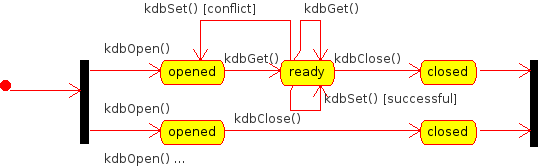
\includegraphics[width=\textwidth,height=\textheight/2,keepaspectratio=true]{state.png}
\doxyfigcaption{State}
\end{DoxyImage}
 As we see in the figure, \hyperlink{group__kdb_ga6808defe5870f328dd17910aacbdc6ca}{kdb\+Open()} can be called arbitrarily often in any number of threads.

For every handle you got from \hyperlink{group__kdb_ga6808defe5870f328dd17910aacbdc6ca}{kdb\+Open()}, for every parent\+Key with a different name, {\itshape only} the shown state transitions are valid. From a freshly opened K\+DB, only \hyperlink{group__kdb_ga28e385fd9cb7ccfe0b2f1ed2f62453a1}{kdb\+Get()} and \hyperlink{group__kdb_gadb54dc9fda17ee07deb9444df745c96f}{kdb\+Close()} are allowed, because otherwise conflicts (error 30) would not be detected.

Once \hyperlink{group__kdb_ga28e385fd9cb7ccfe0b2f1ed2f62453a1}{kdb\+Get()} was called (for a specific handle+parent\+Key), any number of \hyperlink{group__kdb_ga28e385fd9cb7ccfe0b2f1ed2f62453a1}{kdb\+Get()} and \hyperlink{group__kdb_ga11436b058408f83d303ca5e996832bcf}{kdb\+Set()} can be used with this handle respective parent\+Key, unless \hyperlink{group__kdb_ga11436b058408f83d303ca5e996832bcf}{kdb\+Set()} had a conflict (error 30) with another application. Every affair with K\+DB needs to be finished with \hyperlink{group__kdb_gadb54dc9fda17ee07deb9444df745c96f}{kdb\+Close()}.

The name of the parent\+Key in \hyperlink{group__kdb_ga6808defe5870f328dd17910aacbdc6ca}{kdb\+Open()} and \hyperlink{group__kdb_gadb54dc9fda17ee07deb9444df745c96f}{kdb\+Close()} does not matter.

In the usual case we just have one parent\+Key and one handle. In these cases we just have to remember to use \hyperlink{group__kdb_ga28e385fd9cb7ccfe0b2f1ed2f62453a1}{kdb\+Get()} before \hyperlink{group__kdb_ga11436b058408f83d303ca5e996832bcf}{kdb\+Set()}\+:


\begin{DoxyCodeInclude}

\textcolor{preprocessor}{#include <kdb.h>}

\textcolor{keywordtype}{int} \hyperlink{testio__doc_8c_a3c04138a5bfe5d72780bb7e82a18e627}{main} (\textcolor{keywordtype}{void})
\{
        KeySet * myConfig = \hyperlink{group__keyset_ga671e1aaee3ae9dc13b4834a4ddbd2c3c}{ksNew} (0, \hyperlink{kdbenum_8c_a7a28fce3773b2c873c94ac80b8b4cd54}{KS\_END});
        Key * parentKey = \hyperlink{group__key_gad23c65b44bf48d773759e1f9a4d43b89}{keyNew} (\textcolor{stringliteral}{"/sw/MyApp"}, \hyperlink{group__key_gga91fb3178848bd682000958089abbaf40afc1567f74444ff9c219f7456b652b4ec}{KEY\_CASCADING\_NAME}, 
      \hyperlink{group__key_gga91fb3178848bd682000958089abbaf40aa8adb6fcb92dec58fb19410eacfdd403}{KEY\_END});
        KDB * handle = \hyperlink{group__kdb_ga6808defe5870f328dd17910aacbdc6ca}{kdbOpen} (parentKey);

        \hyperlink{group__kdb_ga28e385fd9cb7ccfe0b2f1ed2f62453a1}{kdbGet} (handle, myConfig, parentKey); \textcolor{comment}{// kdbGet() must be first}
        \textcolor{comment}{// now any number of any kdbGet()/kdbSet() calls are allowed, e.g.:}
        \hyperlink{group__kdb_ga11436b058408f83d303ca5e996832bcf}{kdbSet} (handle, myConfig, parentKey);

        \hyperlink{group__keyset_ga27e5c16473b02a422238c8d970db7ac8}{ksDel} (myConfig); \textcolor{comment}{// delete the in-memory configuration}

        \hyperlink{group__kdb_gadb54dc9fda17ee07deb9444df745c96f}{kdbClose} (handle, parentKey); \textcolor{comment}{// no more affairs with the key database.}
        \hyperlink{group__key_ga3df95bbc2494e3e6703ece5639be5bb1}{keyDel} (parentKey);          \textcolor{comment}{// working with key/ks does not need kdb}
\}
\end{DoxyCodeInclude}


To output warnings, you can use following code\+:


\begin{DoxyCodeInclude}
        \textcolor{keyword}{const} Key * metaWarnings = \hyperlink{group__keymeta_ga9ed3875495ddb3d8a8d29158a60a147c}{keyGetMeta} (warningKey, \textcolor{stringliteral}{"warnings"});
        \textcolor{keywordflow}{if} (!metaWarnings) \textcolor{keywordflow}{return} 1; \textcolor{comment}{/* There are no current warnings */}

        \textcolor{keywordtype}{int} nrWarnings = atoi (\hyperlink{group__keyvalue_ga880936f2481d28e6e2acbe7486a21d05}{keyString} (metaWarnings));

        printf (\textcolor{stringliteral}{"There are %d warnings\(\backslash\)n"}, nrWarnings + 1);
        \textcolor{keywordflow}{for} (\textcolor{keywordtype}{int} i = 0; i <= nrWarnings; ++i)
        \{
                \textcolor{keywordtype}{char} buffer[] = \textcolor{stringliteral}{"warnings/#00\(\backslash\)0description"};
                buffer[10] = i / 10 % 10 + \textcolor{charliteral}{'0'};
                buffer[11] = i % 10 + \textcolor{charliteral}{'0'};
                printf (\textcolor{stringliteral}{"buffer is: %s\(\backslash\)n"}, buffer);
                strncat (buffer, \textcolor{stringliteral}{"/number"}, \textcolor{keyword}{sizeof} (buffer) - strlen (buffer) - 1);
                printf (\textcolor{stringliteral}{"number: %s\(\backslash\)n"}, \hyperlink{group__keyvalue_ga880936f2481d28e6e2acbe7486a21d05}{keyString} (\hyperlink{group__keymeta_ga9ed3875495ddb3d8a8d29158a60a147c}{keyGetMeta} (warningKey, buffer)));
                buffer[12] = \textcolor{charliteral}{'\(\backslash\)0'};
                strncat (buffer, \textcolor{stringliteral}{"/description"}, \textcolor{keyword}{sizeof} (buffer) - strlen (buffer) - 1);
                printf (\textcolor{stringliteral}{"description: %s\(\backslash\)n"}, \hyperlink{group__keyvalue_ga880936f2481d28e6e2acbe7486a21d05}{keyString} (\hyperlink{group__keymeta_ga9ed3875495ddb3d8a8d29158a60a147c}{keyGetMeta} (warningKey, buffer))
      );
                buffer[12] = \textcolor{charliteral}{'\(\backslash\)0'};
                strncat (buffer, \textcolor{stringliteral}{"/module"}, \textcolor{keyword}{sizeof} (buffer) - strlen (buffer) - 1);
                \hyperlink{group__keymeta_ga9ed3875495ddb3d8a8d29158a60a147c}{keyGetMeta} (warningKey, buffer);
                printf (\textcolor{stringliteral}{"module: %s\(\backslash\)n"}, \hyperlink{group__keyvalue_ga880936f2481d28e6e2acbe7486a21d05}{keyString} (\hyperlink{group__keymeta_ga9ed3875495ddb3d8a8d29158a60a147c}{keyGetMeta} (warningKey, buffer)));
                buffer[12] = \textcolor{charliteral}{'\(\backslash\)0'};
                strncat (buffer, \textcolor{stringliteral}{"/file"}, \textcolor{keyword}{sizeof} (buffer) - strlen (buffer) - 1);
                \hyperlink{group__keymeta_ga9ed3875495ddb3d8a8d29158a60a147c}{keyGetMeta} (warningKey, buffer);
                printf (\textcolor{stringliteral}{"file: %s\(\backslash\)n"}, \hyperlink{group__keyvalue_ga880936f2481d28e6e2acbe7486a21d05}{keyString} (\hyperlink{group__keymeta_ga9ed3875495ddb3d8a8d29158a60a147c}{keyGetMeta} (warningKey, buffer)));
                buffer[12] = \textcolor{charliteral}{'\(\backslash\)0'};
                strncat (buffer, \textcolor{stringliteral}{"/line"}, \textcolor{keyword}{sizeof} (buffer) - strlen (buffer) - 1);
                \hyperlink{group__keymeta_ga9ed3875495ddb3d8a8d29158a60a147c}{keyGetMeta} (warningKey, buffer);
                printf (\textcolor{stringliteral}{"line: %s\(\backslash\)n"}, \hyperlink{group__keyvalue_ga880936f2481d28e6e2acbe7486a21d05}{keyString} (\hyperlink{group__keymeta_ga9ed3875495ddb3d8a8d29158a60a147c}{keyGetMeta} (warningKey, buffer)));
                buffer[12] = \textcolor{charliteral}{'\(\backslash\)0'};
                strncat (buffer, \textcolor{stringliteral}{"/reason"}, \textcolor{keyword}{sizeof} (buffer) - strlen (buffer) - 1);
                \hyperlink{group__keymeta_ga9ed3875495ddb3d8a8d29158a60a147c}{keyGetMeta} (warningKey, buffer);
                printf (\textcolor{stringliteral}{"reason: %s\(\backslash\)n"}, \hyperlink{group__keyvalue_ga880936f2481d28e6e2acbe7486a21d05}{keyString} (\hyperlink{group__keymeta_ga9ed3875495ddb3d8a8d29158a60a147c}{keyGetMeta} (warningKey, buffer)));
                buffer[12] = \textcolor{charliteral}{'\(\backslash\)0'};
                strncat (buffer, \textcolor{stringliteral}{"/mountpoint"}, \textcolor{keyword}{sizeof} (buffer) - strlen (buffer) - 1);
                \hyperlink{group__keymeta_ga9ed3875495ddb3d8a8d29158a60a147c}{keyGetMeta} (warningKey, buffer);
                printf (\textcolor{stringliteral}{"reason: %s\(\backslash\)n"}, \hyperlink{group__keyvalue_ga880936f2481d28e6e2acbe7486a21d05}{keyString} (\hyperlink{group__keymeta_ga9ed3875495ddb3d8a8d29158a60a147c}{keyGetMeta} (warningKey, buffer)));
                buffer[12] = \textcolor{charliteral}{'\(\backslash\)0'};
                strncat (buffer, \textcolor{stringliteral}{"/configfile"}, \textcolor{keyword}{sizeof} (buffer) - strlen (buffer) - 1);
                \hyperlink{group__keymeta_ga9ed3875495ddb3d8a8d29158a60a147c}{keyGetMeta} (warningKey, buffer);
                printf (\textcolor{stringliteral}{"reason: %s\(\backslash\)n"}, \hyperlink{group__keyvalue_ga880936f2481d28e6e2acbe7486a21d05}{keyString} (\hyperlink{group__keymeta_ga9ed3875495ddb3d8a8d29158a60a147c}{keyGetMeta} (warningKey, buffer)));
        \}
\end{DoxyCodeInclude}
 To output the error, you can use following code\+:


\begin{DoxyCodeInclude}
        \textcolor{keyword}{const} Key * metaError = \hyperlink{group__keymeta_ga9ed3875495ddb3d8a8d29158a60a147c}{keyGetMeta} (errorKey, \textcolor{stringliteral}{"error"});
        \textcolor{keywordflow}{if} (!metaError) \textcolor{keywordflow}{return} 1; \textcolor{comment}{/* There is no current error */}

        printf (\textcolor{stringliteral}{"number: %s\(\backslash\)n"}, \hyperlink{group__keyvalue_ga880936f2481d28e6e2acbe7486a21d05}{keyString} (\hyperlink{group__keymeta_ga9ed3875495ddb3d8a8d29158a60a147c}{keyGetMeta} (errorKey, \textcolor{stringliteral}{"error/number"})));
        printf (\textcolor{stringliteral}{"description: : %s\(\backslash\)n"}, \hyperlink{group__keyvalue_ga880936f2481d28e6e2acbe7486a21d05}{keyString} (\hyperlink{group__keymeta_ga9ed3875495ddb3d8a8d29158a60a147c}{keyGetMeta} (errorKey, \textcolor{stringliteral}{"
      error/description"})));
        printf (\textcolor{stringliteral}{"module: : %s\(\backslash\)n"}, \hyperlink{group__keyvalue_ga880936f2481d28e6e2acbe7486a21d05}{keyString} (\hyperlink{group__keymeta_ga9ed3875495ddb3d8a8d29158a60a147c}{keyGetMeta} (errorKey, \textcolor{stringliteral}{"error/module"})));
        printf (\textcolor{stringliteral}{"at: %s:%s\(\backslash\)n"}, \hyperlink{group__keyvalue_ga880936f2481d28e6e2acbe7486a21d05}{keyString} (\hyperlink{group__keymeta_ga9ed3875495ddb3d8a8d29158a60a147c}{keyGetMeta} (errorKey, \textcolor{stringliteral}{"error/file"})), 
      \hyperlink{group__keyvalue_ga880936f2481d28e6e2acbe7486a21d05}{keyString} (\hyperlink{group__keymeta_ga9ed3875495ddb3d8a8d29158a60a147c}{keyGetMeta} (errorKey, \textcolor{stringliteral}{"error/line"})));
        printf (\textcolor{stringliteral}{"reason: : %s\(\backslash\)n"}, \hyperlink{group__keyvalue_ga880936f2481d28e6e2acbe7486a21d05}{keyString} (\hyperlink{group__keymeta_ga9ed3875495ddb3d8a8d29158a60a147c}{keyGetMeta} (errorKey, \textcolor{stringliteral}{"error/reason"})));
        printf (\textcolor{stringliteral}{"mountpoint: : %s\(\backslash\)n"}, \hyperlink{group__keyvalue_ga880936f2481d28e6e2acbe7486a21d05}{keyString} (\hyperlink{group__keymeta_ga9ed3875495ddb3d8a8d29158a60a147c}{keyGetMeta} (errorKey, \textcolor{stringliteral}{"error/mountpoint
      "})));
        printf (\textcolor{stringliteral}{"configfile: : %s\(\backslash\)n"}, \hyperlink{group__keyvalue_ga880936f2481d28e6e2acbe7486a21d05}{keyString} (\hyperlink{group__keymeta_ga9ed3875495ddb3d8a8d29158a60a147c}{keyGetMeta} (errorKey, \textcolor{stringliteral}{"error/configfile
      "})));
\end{DoxyCodeInclude}


\subsection{Function Documentation}
\mbox{\Hypertarget{group__kdb_gadb54dc9fda17ee07deb9444df745c96f}\label{group__kdb_gadb54dc9fda17ee07deb9444df745c96f}} 
\index{K\+DB@{K\+DB}!kdb\+Close@{kdb\+Close}}
\index{kdb\+Close@{kdb\+Close}!K\+DB@{K\+DB}}
\subsubsection{\texorpdfstring{kdb\+Close()}{kdbClose()}}
{\footnotesize\ttfamily int kdb\+Close (\begin{DoxyParamCaption}\item[{K\+DB $\ast$}]{handle,  }\item[{Key $\ast$}]{error\+Key }\end{DoxyParamCaption})}



Closes the session with the Key database. 

\begin{DoxyPrecond}{Precondition}
The handle must be a valid handle as returned from \hyperlink{group__kdb_ga6808defe5870f328dd17910aacbdc6ca}{kdb\+Open()}

error\+Key must be a valid key, e.\+g. created with \hyperlink{group__key_gad23c65b44bf48d773759e1f9a4d43b89}{key\+New()}
\end{DoxyPrecond}
This is the counterpart of \hyperlink{group__kdb_ga6808defe5870f328dd17910aacbdc6ca}{kdb\+Open()}.

You must call this method when you finished your affairs with the key database. You can manipulate Key and Key\+Set objects also after \hyperlink{group__kdb_gadb54dc9fda17ee07deb9444df745c96f}{kdb\+Close()}, but you must not use any kdb$\ast$() call afterwards.

The {\ttfamily handle} parameter will be finalized and all resources associated to it will be freed. After a \hyperlink{group__kdb_gadb54dc9fda17ee07deb9444df745c96f}{kdb\+Close()}, the {\ttfamily handle} cannot be used anymore.


\begin{DoxyParams}{Parameters}
{\em handle} & contains internal information of \hyperlink{group__kdb_ga6808defe5870f328dd17910aacbdc6ca}{opened } key database \\
\hline
{\em error\+Key} & the key which holds error/warning information \\
\hline
\end{DoxyParams}

\begin{DoxyRetVals}{Return values}
{\em 0} & on success \\
\hline
{\em -\/1} & on N\+U\+LL pointer \\
\hline
\end{DoxyRetVals}
\mbox{\Hypertarget{group__kdb_ga0955373877575fa21275891518f8ab31}\label{group__kdb_ga0955373877575fa21275891518f8ab31}} 
\index{K\+DB@{K\+DB}!kdb\+Ensure@{kdb\+Ensure}}
\index{kdb\+Ensure@{kdb\+Ensure}!K\+DB@{K\+DB}}
\subsubsection{\texorpdfstring{kdb\+Ensure()}{kdbEnsure()}}
{\footnotesize\ttfamily int kdb\+Ensure (\begin{DoxyParamCaption}\item[{K\+DB $\ast$}]{handle,  }\item[{Key\+Set $\ast$}]{contract,  }\item[{Key $\ast$}]{parent\+Key }\end{DoxyParamCaption})}



This function can be used the given K\+DB {\ttfamily handle} meets certain clauses, specified in {\ttfamily contract}. 

Currently the following clauses are supported\+:


\begin{DoxyItemize}
\item {\ttfamily system/elektra/ensure/plugins/$<$mountpoint$>$/$<$pluginname$>$} defines the state of the plugin {\ttfamily $<$pluginname$>$} for the mountpoint {\ttfamily $<$mountpoint$>$}\+:
\begin{DoxyItemize}
\item The value {\ttfamily unmounted} ensures the plugin is not mounted, at this mountpoint.
\item The value {\ttfamily mounted} ensures the plugin is mounted, at this mountpoint. If the plugin is not mounted, we will try to mount it.
\item The value {\ttfamily remount} always mounts the plugin, at this mountpoint. If it was already mounted, it will me unmounted and mounted again. This can be used to ensure the plugin is mounted with a certain configuration.
\end{DoxyItemize}
\item Keys below {\ttfamily system/elektra/ensure/plugins/$<$mountpoint$>$/$<$pluginname$>$/config} are extracted and used as the plugins config Key\+Set during mounting. {\ttfamily system/elektra/ensure/plugins/$<$mountpoint$>$/$<$pluginname$>$} will be repleced by {\ttfamily user} in the keynames. If no keys are given, an empty Key\+Set is used.
\end{DoxyItemize}

There are a few special values for {\ttfamily $<$mountpoint$>$}\+:
\begin{DoxyItemize}
\item {\ttfamily global} is used to indicate the plugin should (un)mounted as a global plugin. Currently this only supports (un)mounting plugins from/to the subposition {\ttfamily maxonce}.
\item {\ttfamily parent} is used to indicate the keyname of {\ttfamily parent\+Key} shall be used as the mountpoint.
\end{DoxyItemize}

If {\ttfamily $<$mountpoint$>$} is none of those values, it has to be valid keyname with the slashes escaped. That means it has to start with {\ttfamily /}, {\ttfamily user}, {\ttfamily system}, {\ttfamily dir} or {\ttfamily spec}.

If {\ttfamily $<$mountpoint$>$} is N\+OT {\ttfamily global}, currently only {\ttfamily unmounted} is supported (not {\ttfamily mounted} and {\ttfamily remounted}).

N\+O\+TE\+: This function only works properly, if the list plugin is mounted in all global positions. If this is not the case, 1 will be returned, because this is seen as an implicit clause in the contract. Additionally any contract that specifies clauses for the list plugin is rejected as malformed.


\begin{DoxyParams}{Parameters}
{\em handle} & contains internal information of \hyperlink{group__kdb_ga6808defe5870f328dd17910aacbdc6ca}{opened } key database \\
\hline
{\em contract} & Key\+Set containing the contract described above. This will always be {\ttfamily \hyperlink{group__keyset_ga27e5c16473b02a422238c8d970db7ac8}{ks\+Del()}}ed. {\bfseries Even in error cases.} \\
\hline
{\em parent\+Key} & The parent\+Key used if the {\ttfamily parent} special value is used, otherwise only used for error reporting.\\
\hline
\end{DoxyParams}

\begin{DoxyRetVals}{Return values}
{\em 0} & on success \\
\hline
{\em 1} & if clauses of the contract are unmet \\
\hline
{\em -\/1} & on N\+U\+LL pointers, or malformed contract \\
\hline
\end{DoxyRetVals}
\mbox{\Hypertarget{group__kdb_ga28e385fd9cb7ccfe0b2f1ed2f62453a1}\label{group__kdb_ga28e385fd9cb7ccfe0b2f1ed2f62453a1}} 
\index{K\+DB@{K\+DB}!kdb\+Get@{kdb\+Get}}
\index{kdb\+Get@{kdb\+Get}!K\+DB@{K\+DB}}
\subsubsection{\texorpdfstring{kdb\+Get()}{kdbGet()}}
{\footnotesize\ttfamily int kdb\+Get (\begin{DoxyParamCaption}\item[{K\+DB $\ast$}]{handle,  }\item[{Key\+Set $\ast$}]{ks,  }\item[{Key $\ast$}]{parent\+Key }\end{DoxyParamCaption})}



Retrieve keys in an atomic and universal way. 

\begin{DoxyPrecond}{Precondition}
The {\ttfamily handle} must be passed as returned from \hyperlink{group__kdb_ga6808defe5870f328dd17910aacbdc6ca}{kdb\+Open()}.

The {\ttfamily returned} Key\+Set must be a valid Key\+Set, e.\+g. constructed with \hyperlink{group__keyset_ga671e1aaee3ae9dc13b4834a4ddbd2c3c}{ks\+New()}.

The {\ttfamily parent\+Key} Key must be a valid Key, e.\+g. constructed with \hyperlink{group__key_gad23c65b44bf48d773759e1f9a4d43b89}{key\+New()}.
\end{DoxyPrecond}
If you pass N\+U\+LL on any parameter \hyperlink{group__kdb_ga28e385fd9cb7ccfe0b2f1ed2f62453a1}{kdb\+Get()} will fail immediately without doing anything.

The {\ttfamily returned} Key\+Set may already contain some keys, e.\+g. from previous \hyperlink{group__kdb_ga28e385fd9cb7ccfe0b2f1ed2f62453a1}{kdb\+Get()} calls. The new retrieved keys will be appended using \hyperlink{group__keyset_gaa5a1d467a4d71041edce68ea7748ce45}{ks\+Append\+Key()}.

If not done earlier \hyperlink{group__kdb_ga28e385fd9cb7ccfe0b2f1ed2f62453a1}{kdb\+Get()} will fully retrieve all keys under the {\ttfamily parent\+Key} folder recursively (See Optimization below when it will not be done).

\begin{DoxyNote}{Note}
\hyperlink{group__kdb_ga28e385fd9cb7ccfe0b2f1ed2f62453a1}{kdb\+Get()} might retrieve more keys than requested (that are not below parent\+Key). These keys must be passed to calls of \hyperlink{group__kdb_ga11436b058408f83d303ca5e996832bcf}{kdb\+Set()}, otherwise they will be lost. This stems from the fact that the user has the only copy of the whole configuration and backends only write configuration that was passed to them. For example, if you \hyperlink{group__kdb_ga28e385fd9cb7ccfe0b2f1ed2f62453a1}{kdb\+Get()} \char`\"{}system/mountpoint/interest\char`\"{} you will not only get all keys below system/mountpoint/interest, but also all keys below system/mountpoint (if system/mountpoint is a mountpoint as the name suggests, but system/mountpoint/interest is not a mountpoint). Make sure to not touch or remove keys outside the keys of interest, because others may need them!
\end{DoxyNote}
\begin{DoxyParagraph}{Example\+:}
This example demonstrates the typical usecase within an application (without error handling).
\end{DoxyParagraph}

\begin{DoxyCodeInclude}

\textcolor{preprocessor}{#include <kdb.h>}
\textcolor{preprocessor}{#include <stdio.h>}

\textcolor{keywordtype}{int} \hyperlink{testio__doc_8c_a3c04138a5bfe5d72780bb7e82a18e627}{main} (\textcolor{keywordtype}{void})
\{
        KeySet * myConfig = \hyperlink{group__keyset_ga671e1aaee3ae9dc13b4834a4ddbd2c3c}{ksNew} (0, \hyperlink{kdbenum_8c_a7a28fce3773b2c873c94ac80b8b4cd54}{KS\_END});

        \textcolor{comment}{// for error handling see kdbget\_error.c}

        \textcolor{comment}{// clang-format off}
\textcolor{comment}{}Key * key = \hyperlink{group__key_gad23c65b44bf48d773759e1f9a4d43b89}{keyNew} (\textcolor{stringliteral}{"/sw/tests/myapp/#0/current/"},  \hyperlink{group__key_gga91fb3178848bd682000958089abbaf40aa8adb6fcb92dec58fb19410eacfdd403}{KEY\_END});
KDB * handle = \hyperlink{group__kdb_ga6808defe5870f328dd17910aacbdc6ca}{kdbOpen} (key);
\hyperlink{group__kdb_ga28e385fd9cb7ccfe0b2f1ed2f62453a1}{kdbGet} (handle, myConfig, key);
Key * result = \hyperlink{group__keyset_gad2e30fb6d4739d917c5abb2ac2f9c1a1}{ksLookupByName} (myConfig, \textcolor{stringliteral}{"/sw/tests/myapp/#0/current/testkey1"}, 0);
        \textcolor{comment}{// clang-format on}

        \hyperlink{group__key_ga3df95bbc2494e3e6703ece5639be5bb1}{keyDel} (key);

        \textcolor{keyword}{const} \textcolor{keywordtype}{char} * key\_name = \hyperlink{group__keyname_ga8e805c726a60da921d3736cda7813513}{keyName} (result);
        \textcolor{keyword}{const} \textcolor{keywordtype}{char} * key\_value = \hyperlink{group__keyvalue_ga880936f2481d28e6e2acbe7486a21d05}{keyString} (result);
        \textcolor{keyword}{const} \textcolor{keywordtype}{char} * key\_comment = \hyperlink{group__keyvalue_ga880936f2481d28e6e2acbe7486a21d05}{keyString} (\hyperlink{group__keymeta_ga9ed3875495ddb3d8a8d29158a60a147c}{keyGetMeta} (result, \textcolor{stringliteral}{"comment"}));
        printf (\textcolor{stringliteral}{"key: %s value: %s comment: %s\(\backslash\)n"}, key\_name, key\_value, key\_comment);

        \hyperlink{group__keyset_ga27e5c16473b02a422238c8d970db7ac8}{ksDel} (myConfig); \textcolor{comment}{// delete the in-memory configuration}


        \textcolor{comment}{// maybe you want kdbSet() myConfig here}

        \hyperlink{group__kdb_gadb54dc9fda17ee07deb9444df745c96f}{kdbClose} (handle, 0); \textcolor{comment}{// no more affairs with the key database.}
\}
\end{DoxyCodeInclude}


When a backend fails \hyperlink{group__kdb_ga28e385fd9cb7ccfe0b2f1ed2f62453a1}{kdb\+Get()} will return -\/1 with all error and warning information in the {\ttfamily parent\+Key}. The parameter {\ttfamily returned} will not be changed.

\begin{DoxyParagraph}{Optimization\+:}
In the first run of kdb\+Get all requested (or more) keys are retrieved. On subsequent calls only the keys are retrieved where something was changed inside the key database. The other keys stay in the Key\+Set returned as passed.
\end{DoxyParagraph}
It is your responsibility to save the original keyset if you need it afterwards.

If you want to be sure to get a fresh keyset again, you need to open a second handle to the key database using \hyperlink{group__kdb_ga6808defe5870f328dd17910aacbdc6ca}{kdb\+Open()}.


\begin{DoxyParams}{Parameters}
{\em handle} & contains internal information of \hyperlink{group__kdb_ga6808defe5870f328dd17910aacbdc6ca}{opened } key database \\
\hline
{\em parent\+Key} & is used to add warnings and set an error information. Additionally, its name is a hint which keys should be retrieved (it is possible that more are retrieved, see Note above).
\begin{DoxyItemize}
\item cascading keys (starting with /) will retrieve the same path in all namespaces
\item / will retrieve all keys 
\end{DoxyItemize}\\
\hline
{\em ks} & the (pre-\/initialized) Key\+Set returned with all keys found will not be changed on error or if no update is required \\
\hline
\end{DoxyParams}
\begin{DoxySeeAlso}{See also}
\hyperlink{group__keyset_gaa34fc43a081e6b01e4120daa6c112004}{ks\+Lookup()}, \hyperlink{group__keyset_gad2e30fb6d4739d917c5abb2ac2f9c1a1}{ks\+Lookup\+By\+Name()} for powerful lookups after the Key\+Set was retrieved 

\hyperlink{group__kdb_ga6808defe5870f328dd17910aacbdc6ca}{kdb\+Open()} which needs to be called before 

\hyperlink{group__kdb_ga11436b058408f83d303ca5e996832bcf}{kdb\+Set()} to save the configuration afterwards and \hyperlink{group__kdb_gadb54dc9fda17ee07deb9444df745c96f}{kdb\+Close()} to finish affairs with the \hyperlink{group__key}{Key} database. 
\end{DoxySeeAlso}

\begin{DoxyRetVals}{Return values}
{\em 1} & if the keys were retrieved successfully \\
\hline
{\em 0} & if there was no update -\/ no changes are made to the keyset then \\
\hline
{\em -\/1} & on failure -\/ no changes are made to the keyset then \\
\hline
\end{DoxyRetVals}
\mbox{\Hypertarget{group__kdb_ga6808defe5870f328dd17910aacbdc6ca}\label{group__kdb_ga6808defe5870f328dd17910aacbdc6ca}} 
\index{K\+DB@{K\+DB}!kdb\+Open@{kdb\+Open}}
\index{kdb\+Open@{kdb\+Open}!K\+DB@{K\+DB}}
\subsubsection{\texorpdfstring{kdb\+Open()}{kdbOpen()}}
{\footnotesize\ttfamily K\+DB$\ast$ kdb\+Open (\begin{DoxyParamCaption}\item[{Key $\ast$}]{error\+Key }\end{DoxyParamCaption})}



Opens the session with the Key database. 

\begin{DoxyPrecond}{Precondition}
error\+Key must be a valid key, e.\+g. created with \hyperlink{group__key_gad23c65b44bf48d773759e1f9a4d43b89}{key\+New()}
\end{DoxyPrecond}
The method will bootstrap itself the following way. The first step is to open the default backend. With it system/elektra/mountpoints will be loaded and all needed libraries and mountpoints will be determined. These libraries for backends will be loaded and with it the {\ttfamily K\+DB} data structure will be initialized.

You must always call this method before retrieving or committing any keys to the database. In the end of the program, after using the key database, you must not forget to \hyperlink{group__kdb_gadb54dc9fda17ee07deb9444df745c96f}{kdb\+Close()}.

The pointer to the {\ttfamily K\+DB} structure returned will be initialized like described above, and it must be passed along on any kdb$\ast$() method your application calls.

Get a {\ttfamily K\+DB} handle for every thread using elektra. Don\textquotesingle{}t share the handle across threads, and also not the pointer accessing it\+:


\begin{DoxyCodeInclude}
\textcolor{keywordtype}{void} thread1 (\textcolor{keywordtype}{void})
\{
        Key * parent = \hyperlink{group__key_gad23c65b44bf48d773759e1f9a4d43b89}{keyNew} (\textcolor{stringliteral}{"/app/part1"}, \hyperlink{group__key_gga91fb3178848bd682000958089abbaf40afc1567f74444ff9c219f7456b652b4ec}{KEY\_CASCADING\_NAME}, 
      \hyperlink{group__key_gga91fb3178848bd682000958089abbaf40aa8adb6fcb92dec58fb19410eacfdd403}{KEY\_END});
        KDB * h = \hyperlink{group__kdb_ga6808defe5870f328dd17910aacbdc6ca}{kdbOpen} (parent);
        \textcolor{comment}{// fetch keys and work with them}
        \hyperlink{group__kdb_gadb54dc9fda17ee07deb9444df745c96f}{kdbClose} (h, parent);
\}
\textcolor{keywordtype}{void} thread2 (\textcolor{keywordtype}{void})
\{
        Key * parent = \hyperlink{group__key_gad23c65b44bf48d773759e1f9a4d43b89}{keyNew} (\textcolor{stringliteral}{"/app/part2"}, \hyperlink{group__key_gga91fb3178848bd682000958089abbaf40afc1567f74444ff9c219f7456b652b4ec}{KEY\_CASCADING\_NAME}, 
      \hyperlink{group__key_gga91fb3178848bd682000958089abbaf40aa8adb6fcb92dec58fb19410eacfdd403}{KEY\_END});
        KDB * h = \hyperlink{group__kdb_ga6808defe5870f328dd17910aacbdc6ca}{kdbOpen} (parent);
        \textcolor{comment}{// fetch keys and work with them}
        \hyperlink{group__kdb_gadb54dc9fda17ee07deb9444df745c96f}{kdbClose} (h, parent);
\}
\end{DoxyCodeInclude}
 You don\textquotesingle{}t need \hyperlink{group__kdb_ga6808defe5870f328dd17910aacbdc6ca}{kdb\+Open()} if you only want to manipulate plain in-\/memory Key or Key\+Set objects.

\begin{DoxyPrecond}{Precondition}
error\+Key must be a valid key, e.\+g. created with \hyperlink{group__key_gad23c65b44bf48d773759e1f9a4d43b89}{key\+New()}
\end{DoxyPrecond}

\begin{DoxyParams}{Parameters}
{\em error\+Key} & the key which holds errors and warnings which were issued \\
\hline
\end{DoxyParams}
\begin{DoxySeeAlso}{See also}
\hyperlink{group__kdb_ga28e385fd9cb7ccfe0b2f1ed2f62453a1}{kdb\+Get()}, \hyperlink{group__kdb_gadb54dc9fda17ee07deb9444df745c96f}{kdb\+Close()} to end all affairs to the \hyperlink{group__key}{Key} database. 
\end{DoxySeeAlso}

\begin{DoxyRetVals}{Return values}
{\em handle} & on success \\
\hline
{\em N\+U\+LL} & on failure \\
\hline
\end{DoxyRetVals}
\mbox{\Hypertarget{group__kdb_ga11436b058408f83d303ca5e996832bcf}\label{group__kdb_ga11436b058408f83d303ca5e996832bcf}} 
\index{K\+DB@{K\+DB}!kdb\+Set@{kdb\+Set}}
\index{kdb\+Set@{kdb\+Set}!K\+DB@{K\+DB}}
\subsubsection{\texorpdfstring{kdb\+Set()}{kdbSet()}}
{\footnotesize\ttfamily int kdb\+Set (\begin{DoxyParamCaption}\item[{K\+DB $\ast$}]{handle,  }\item[{Key\+Set $\ast$}]{ks,  }\item[{Key $\ast$}]{parent\+Key }\end{DoxyParamCaption})}



Set keys in an atomic and universal way. 

\begin{DoxyPrecond}{Precondition}
\hyperlink{group__kdb_ga28e385fd9cb7ccfe0b2f1ed2f62453a1}{kdb\+Get()} must be called before \hyperlink{group__kdb_ga11436b058408f83d303ca5e996832bcf}{kdb\+Set()}\+:
\begin{DoxyItemize}
\item initially (after \hyperlink{group__kdb_ga6808defe5870f328dd17910aacbdc6ca}{kdb\+Open()})
\item after conflict errors in \hyperlink{group__kdb_ga11436b058408f83d303ca5e996832bcf}{kdb\+Set()}.
\end{DoxyItemize}

The {\ttfamily returned} Key\+Set must be a valid Key\+Set, e.\+g. constructed with \hyperlink{group__keyset_ga671e1aaee3ae9dc13b4834a4ddbd2c3c}{ks\+New()}.

The {\ttfamily parent\+Key} Key must be a valid Key, e.\+g. constructed with \hyperlink{group__key_gad23c65b44bf48d773759e1f9a4d43b89}{key\+New()}.
\end{DoxyPrecond}
If you pass N\+U\+LL on any parameter \hyperlink{group__kdb_ga11436b058408f83d303ca5e996832bcf}{kdb\+Set()} will fail immediately without doing anything.

With {\ttfamily parent\+Key} you can give an hint which part of the given keyset is of interest for you. Then you promise to only modify or remove keys below this key. All others would be passed back as they were retrieved by \hyperlink{group__kdb_ga28e385fd9cb7ccfe0b2f1ed2f62453a1}{kdb\+Get()}.

\begin{DoxyParagraph}{Errors}
If some error occurs\+:
\begin{DoxyItemize}
\item \hyperlink{group__kdb_ga11436b058408f83d303ca5e996832bcf}{kdb\+Set()} will leave the Key\+Set\textquotesingle{}s $\ast$ internal cursor on the key that generated the error.
\item Error information will be written into the metadata of the parent key.
\item None of the keys are actually committed in this situation, i.\+e. no configuration file will be modified.
\end{DoxyItemize}
\end{DoxyParagraph}
In case of errors you should present the error message to the user and let the user decide what to do. Possible solutions are\+:
\begin{DoxyItemize}
\item remove the problematic key and use \hyperlink{group__kdb_ga11436b058408f83d303ca5e996832bcf}{kdb\+Set()} again (for validation or type errors)
\item change the value of the problematic key and use \hyperlink{group__kdb_ga11436b058408f83d303ca5e996832bcf}{kdb\+Set()} again (for validation errors)
\item do a \hyperlink{group__kdb_ga28e385fd9cb7ccfe0b2f1ed2f62453a1}{kdb\+Get()} (for conflicts, i.\+e. error 30) and then
\begin{DoxyItemize}
\item set the same keyset again (in favour of what was set by this user)
\item drop the old keyset (in favour of what was set from another application)
\item merge the original, your own and the other keyset
\end{DoxyItemize}
\item export the configuration into a file (for unresolvable errors)
\item repeat the same kdb\+Set might be of limited use if the user does not explicitly request it, because temporary errors are rare and its unlikely that they fix themselves (e.\+g. disc full, permission problems)
\end{DoxyItemize}

\begin{DoxyParagraph}{Optimization}
Each key is checked with \hyperlink{group__keytest_gaf247df0de7aca04b32ef80e39ef12950}{key\+Need\+Sync()} before being actually committed. If no key of a backend needs to be synced any affairs to backends are omitted and 0 is returned.
\end{DoxyParagraph}

\begin{DoxyCodeInclude}
KeySet * myConfig = \hyperlink{group__keyset_ga671e1aaee3ae9dc13b4834a4ddbd2c3c}{ksNew} (0, \hyperlink{kdbenum_8c_a7a28fce3773b2c873c94ac80b8b4cd54}{KS\_END});
Key * parentKey = \hyperlink{group__key_gad23c65b44bf48d773759e1f9a4d43b89}{keyNew} (\textcolor{stringliteral}{"system/sw/MyApp"}, \hyperlink{group__key_gga91fb3178848bd682000958089abbaf40aa8adb6fcb92dec58fb19410eacfdd403}{KEY\_END});
KDB * handle = \hyperlink{group__kdb_ga6808defe5870f328dd17910aacbdc6ca}{kdbOpen} (parentKey);

\hyperlink{group__kdb_ga28e385fd9cb7ccfe0b2f1ed2f62453a1}{kdbGet} (handle, myConfig, parentKey); \textcolor{comment}{// kdbGet needs to be called first!}
KeySet * base = \hyperlink{group__keyset_gac59e4b328245463f1451f68d5106151c}{ksDup} (myConfig);     \textcolor{comment}{// save a copy of original keyset}

\textcolor{comment}{// change the keys within myConfig}

KeySet * ours = \hyperlink{group__keyset_gac59e4b328245463f1451f68d5106151c}{ksDup} (myConfig); \textcolor{comment}{// save a copy of our keyset}
KeySet * theirs;                  \textcolor{comment}{// needed for 3-way merging}
\textcolor{keywordtype}{int} ret = \hyperlink{group__kdb_ga11436b058408f83d303ca5e996832bcf}{kdbSet} (handle, myConfig, parentKey);
\textcolor{keywordflow}{while} (ret == -1) \textcolor{comment}{// as long as we have an error}
\{
        \textcolor{comment}{// We got an error. Warn user.}
        Key * problemKey = \hyperlink{group__keyset_ga4287b9416912c5f2ab9c195cb74fb094}{ksCurrent} (myConfig);
        \textcolor{comment}{// parentKey has the errorInformation}
        \textcolor{comment}{// problemKey is the faulty key (may be null)}
        \textcolor{keywordtype}{int} userInput = showElektraErrorDialog (parentKey, problemKey);
        \textcolor{keywordflow}{switch} (userInput)
        \{
        \textcolor{keywordflow}{case} INPUT\_USE\_OURS:
                \hyperlink{group__kdb_ga28e385fd9cb7ccfe0b2f1ed2f62453a1}{kdbGet} (handle, myConfig, parentKey); \textcolor{comment}{// refresh key database}
                \hyperlink{group__keyset_ga27e5c16473b02a422238c8d970db7ac8}{ksDel} (myConfig);
                myConfig = ours;
                \textcolor{keywordflow}{break};
        \textcolor{keywordflow}{case} INPUT\_DO\_MERGE:
                theirs = \hyperlink{group__keyset_gac59e4b328245463f1451f68d5106151c}{ksDup} (ours);
                \hyperlink{group__kdb_ga28e385fd9cb7ccfe0b2f1ed2f62453a1}{kdbGet} (handle, theirs, parentKey); \textcolor{comment}{// refresh key database}
                KeySet * res = doElektraMerge (ours, theirs, base);
                \hyperlink{group__keyset_ga27e5c16473b02a422238c8d970db7ac8}{ksDel} (theirs);
                myConfig = res;
                \textcolor{keywordflow}{break};
        \textcolor{keywordflow}{case} INPUT\_USE\_THEIRS:
                \textcolor{comment}{// should always work, we just write what we got}
                \textcolor{comment}{// but to be sure always give the user another way}
                \textcolor{comment}{// to exit the loop}
                \hyperlink{group__kdb_ga28e385fd9cb7ccfe0b2f1ed2f62453a1}{kdbGet} (handle, myConfig, parentKey); \textcolor{comment}{// refresh key database}
                \textcolor{keywordflow}{break};
                \textcolor{comment}{// other cases ...}
        \}
        ret = \hyperlink{group__kdb_ga11436b058408f83d303ca5e996832bcf}{kdbSet} (handle, myConfig, parentKey);
\}

\hyperlink{group__keyset_ga27e5c16473b02a422238c8d970db7ac8}{ksDel} (ours);
\hyperlink{group__keyset_ga27e5c16473b02a422238c8d970db7ac8}{ksDel} (base);
\hyperlink{group__keyset_ga27e5c16473b02a422238c8d970db7ac8}{ksDel} (myConfig); \textcolor{comment}{// delete the in-memory configuration}

\hyperlink{group__kdb_gadb54dc9fda17ee07deb9444df745c96f}{kdbClose} (handle, parentKey); \textcolor{comment}{// no more affairs with the key database.}
\hyperlink{group__key_ga3df95bbc2494e3e6703ece5639be5bb1}{keyDel} (parentKey);
\end{DoxyCodeInclude}
 show\+Elektra\+Error\+Dialog() and do\+Elektra\+Merge() need to be implemented by the user of Elektra. For do\+Elektra\+Merge a 3-\/way merge algorithm exists in libelektra-\/tools.


\begin{DoxyParams}{Parameters}
{\em handle} & contains internal information of \hyperlink{group__kdb_ga6808defe5870f328dd17910aacbdc6ca}{opened } key database \\
\hline
{\em ks} & a Key\+Set which should contain changed keys, otherwise nothing is done \\
\hline
{\em parent\+Key} & is used to add warnings and set an error information. Additionally, its name is an hint which keys should be committed (it is possible that more are changed).
\begin{DoxyItemize}
\item cascading keys (starting with /) will set the path in all namespaces
\item / will commit all keys
\item metanames will be rejected (error 104)
\item empty/invalid (error 105) 
\end{DoxyItemize}\\
\hline
\end{DoxyParams}

\begin{DoxyRetVals}{Return values}
{\em 1} & on success \\
\hline
{\em 0} & if nothing had to be done, no changes in K\+DB \\
\hline
{\em -\/1} & on failure, no changes in K\+DB \\
\hline
\end{DoxyRetVals}
\begin{DoxySeeAlso}{See also}
\hyperlink{group__keytest_gaf247df0de7aca04b32ef80e39ef12950}{key\+Need\+Sync()} 

\hyperlink{group__keyset_ga4287b9416912c5f2ab9c195cb74fb094}{ks\+Current()} contains the error \hyperlink{group__key}{Key} 

\hyperlink{group__kdb_ga6808defe5870f328dd17910aacbdc6ca}{kdb\+Open()} and \hyperlink{group__kdb_ga28e385fd9cb7ccfe0b2f1ed2f62453a1}{kdb\+Get()} that must be called first 

\hyperlink{group__kdb_gadb54dc9fda17ee07deb9444df745c96f}{kdb\+Close()} that must be called afterwards 
\end{DoxySeeAlso}

\hypertarget{group__key}{}\doxysection{Key}
\label{group__key}\index{Key@{Key}}


Key is an essential class that encapsulates key \mbox{\hyperlink{group__keyname}{name }}, \mbox{\hyperlink{group__keyvalue}{value }} and \mbox{\hyperlink{group__keymeta}{metainfo }}.  


Collaboration diagram for Key\+:
\nopagebreak
\begin{figure}[H]
\begin{center}
\leavevmode
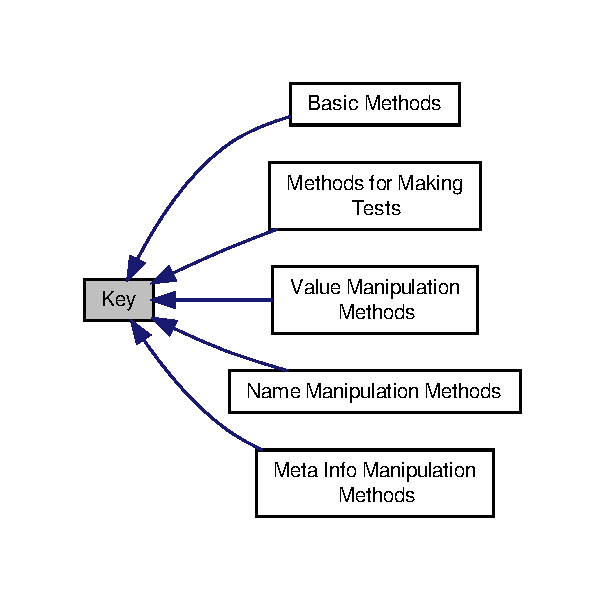
\includegraphics[width=309pt]{group__key}
\end{center}
\end{figure}
\doxysubsection*{Modules}
\begin{DoxyCompactItemize}
\item 
\mbox{\hyperlink{group__keymeta}{Meta Info Manipulation Methods}}
\begin{DoxyCompactList}\small\item\em Methods to do various operations on Key metadata. \end{DoxyCompactList}\item 
\mbox{\hyperlink{group__keytest}{Methods for Making Tests}}
\begin{DoxyCompactList}\small\item\em Methods to do various tests on Keys. \end{DoxyCompactList}\item 
\mbox{\hyperlink{group__keyname}{Name Manipulation Methods}}
\begin{DoxyCompactList}\small\item\em Methods to do various operations on Key names. \end{DoxyCompactList}\item 
\mbox{\hyperlink{group__keyvalue}{Value Manipulation Methods}}
\begin{DoxyCompactList}\small\item\em Methods to do various operations on Key values. \end{DoxyCompactList}\end{DoxyCompactItemize}
\doxysubsection*{Macros}
\begin{DoxyCompactItemize}
\item 
\#define \mbox{\hyperlink{group__key_gad19f92d6d37dc439d1727ca10263c9cc}{KDB\+\_\+\+PATH\+\_\+\+SEPARATOR}}~\textquotesingle{}/\textquotesingle{}
\begin{DoxyCompactList}\small\item\em {\ttfamily /} is used to separate key names. \end{DoxyCompactList}\item 
\#define \mbox{\hyperlink{group__key_ga6d24980bc81c4276367f4e80725a8b61}{KDB\+\_\+\+PATH\+\_\+\+ESCAPE}}~\textquotesingle{}\textbackslash{}\textbackslash{}\textquotesingle{}
\begin{DoxyCompactList}\small\item\em {\ttfamily \textbackslash{}} is used as escape character in the key name. \end{DoxyCompactList}\end{DoxyCompactItemize}
\doxysubsection*{Enumerations}
\begin{DoxyCompactItemize}
\item 
enum \mbox{\hyperlink{group__key_ga9b703ca49f48b482def322b77d3e6bc8}{elektra\+Key\+Flags}} \{ \newline
\mbox{\hyperlink{group__key_gga9b703ca49f48b482def322b77d3e6bc8ad6127fc38f96410bf7c8f6e93b0397da}{KEY\+\_\+\+NAME}} = 1
, \mbox{\hyperlink{group__key_gga9b703ca49f48b482def322b77d3e6bc8ac66e4a49d09212b79f5754ca6db5bd2e}{KEY\+\_\+\+VALUE}} = 1 $<$$<$ 1
, \mbox{\hyperlink{group__key_gga9b703ca49f48b482def322b77d3e6bc8a4b83f86a07a7a0d6e24ecafe43cfea1b}{KEY\+\_\+\+FLAGS}} = 3
, \mbox{\hyperlink{group__key_gga9b703ca49f48b482def322b77d3e6bc8ac29427bb47cc31689d02912e36161ee3}{KEY\+\_\+\+COMMENT}} = 1 $<$$<$ 3
, \newline
\mbox{\hyperlink{group__key_gga9b703ca49f48b482def322b77d3e6bc8a1ca18d4e094ae7487d35ecedda2235ff}{KEY\+\_\+\+BINARY}} = 1 $<$$<$ 4
, \mbox{\hyperlink{group__key_gga9b703ca49f48b482def322b77d3e6bc8a6d531b5c41445d19d0452eebdccbfa01}{KEY\+\_\+\+SIZE}} = 1 $<$$<$ 11
, \mbox{\hyperlink{group__key_gga9b703ca49f48b482def322b77d3e6bc8a040582834bb2d90049947d7ef74e87e2}{KEY\+\_\+\+META}} = 1 $<$$<$ 15
, \mbox{\hyperlink{group__key_gga9b703ca49f48b482def322b77d3e6bc8ab089c5e7977d6e58737eb586ee153b7f}{KEY\+\_\+\+NULL}} = 1 $<$$<$ 16
, \newline
\mbox{\hyperlink{group__key_gga9b703ca49f48b482def322b77d3e6bc8aa8adb6fcb92dec58fb19410eacfdd403}{KEY\+\_\+\+END}} = 0
 \}
\begin{DoxyCompactList}\small\item\em Allows \mbox{\hyperlink{group__key_gad23c65b44bf48d773759e1f9a4d43b89}{key\+New()}} to determine which information comes next. \end{DoxyCompactList}\item 
enum \mbox{\hyperlink{group__key_ga9ff42b1e9a97222562bfda3dd1f8c735}{elektra\+Copy\+Flags}} \{ \newline
\mbox{\hyperlink{group__key_gga9ff42b1e9a97222562bfda3dd1f8c735ab41d70eb97ae5480333e85759318b5a9}{KEY\+\_\+\+CP\+\_\+\+NAME}} = 1 $<$$<$ 0
, \mbox{\hyperlink{group__key_gga9ff42b1e9a97222562bfda3dd1f8c735a57996652569a901d4e7e58c33f7b3631}{KEY\+\_\+\+CP\+\_\+\+STRING}} = 1 $<$$<$ 1
, \mbox{\hyperlink{group__key_gga9ff42b1e9a97222562bfda3dd1f8c735a3043a92bfbe465ccff7624e54d89bcf8}{KEY\+\_\+\+CP\+\_\+\+VALUE}} = 1 $<$$<$ 2
, \mbox{\hyperlink{group__key_gga9ff42b1e9a97222562bfda3dd1f8c735a6b8bdcae98a0f29d66a6b3d1651cbac6}{KEY\+\_\+\+CP\+\_\+\+META}} = 1 $<$$<$ 3
, \newline
\mbox{\hyperlink{group__key_gga9ff42b1e9a97222562bfda3dd1f8c735a3e04e17514f102f1e9217308d44e7612}{KEY\+\_\+\+CP\+\_\+\+ALL}} = KEY\+\_\+\+CP\+\_\+\+NAME $\vert$ KEY\+\_\+\+CP\+\_\+\+VALUE $\vert$ KEY\+\_\+\+CP\+\_\+\+META
 \}
\begin{DoxyCompactList}\small\item\em Copy options. \end{DoxyCompactList}\item 
enum \mbox{\hyperlink{group__key_gafa3306030b1d06b06c3cba24c516f5ec}{elektra\+Lock\+Flags}} \{ \mbox{\hyperlink{group__key_ggafa3306030b1d06b06c3cba24c516f5eca4813b0cfdefeb676e35f599ef763c265}{KEY\+\_\+\+LOCK\+\_\+\+NAME}} = 1 $<$$<$ 17
, \mbox{\hyperlink{group__key_ggafa3306030b1d06b06c3cba24c516f5eca4ed4895f3f243287f7adef621815d7e6}{KEY\+\_\+\+LOCK\+\_\+\+VALUE}} = 1 $<$$<$ 18
, \mbox{\hyperlink{group__key_ggafa3306030b1d06b06c3cba24c516f5eca4f1b7ee5af7539286d8989a9a5658958}{KEY\+\_\+\+LOCK\+\_\+\+META}} = 1 $<$$<$ 19
 \}
\begin{DoxyCompactList}\small\item\em Lock options. \end{DoxyCompactList}\item 
enum \mbox{\hyperlink{group__key_gaec3b8d6f430ae49b91bafe8a86310a68}{elektra\+Namespace}} \{ \newline
\mbox{\hyperlink{group__key_ggaec3b8d6f430ae49b91bafe8a86310a68a3659698b0a07454ca8055ab693e8efd1}{KEY\+\_\+\+NS\+\_\+\+NONE}} = 0
, \mbox{\hyperlink{group__key_ggaec3b8d6f430ae49b91bafe8a86310a68a2c9133e3095dccbcde5ca3bb13987b5d}{KEY\+\_\+\+NS\+\_\+\+CASCADING}} = 1
, \mbox{\hyperlink{group__key_ggaec3b8d6f430ae49b91bafe8a86310a68ac5fbf2c3a7ae79fa2d60c48ae3e72688}{KEY\+\_\+\+NS\+\_\+\+META}} = 2
, \mbox{\hyperlink{group__key_ggaec3b8d6f430ae49b91bafe8a86310a68a2be047b124b1ca0e92b5ef124169f0d2}{KEY\+\_\+\+NS\+\_\+\+SPEC}} = 3
, \newline
\mbox{\hyperlink{group__key_ggaec3b8d6f430ae49b91bafe8a86310a68a470ecc9254fcdfccf9923a3e526c9c11}{KEY\+\_\+\+NS\+\_\+\+PROC}} = 4
, \mbox{\hyperlink{group__key_ggaec3b8d6f430ae49b91bafe8a86310a68aa0006cf27dbb2586bafba6ff1ae4f4ec}{KEY\+\_\+\+NS\+\_\+\+DIR}} = 5
, \mbox{\hyperlink{group__key_ggaec3b8d6f430ae49b91bafe8a86310a68a8ce23c70010e8ac8bb540b0947e03a4e}{KEY\+\_\+\+NS\+\_\+\+USER}} = 6
, \mbox{\hyperlink{group__key_ggaec3b8d6f430ae49b91bafe8a86310a68a61adca2f9dff47e65dfcdb492ffa7a20}{KEY\+\_\+\+NS\+\_\+\+SYSTEM}} = 7
, \newline
\mbox{\hyperlink{group__key_ggaec3b8d6f430ae49b91bafe8a86310a68ad6792ab14711ed6d6e507ca3d10b05e7}{KEY\+\_\+\+NS\+\_\+\+DEFAULT}} = 8
 \}
\begin{DoxyCompactList}\small\item\em Elektra currently supported Key namespaces. \end{DoxyCompactList}\end{DoxyCompactItemize}
\doxysubsection*{Functions}
\begin{DoxyCompactItemize}
\item 
Key $\ast$ \mbox{\hyperlink{group__key_gad23c65b44bf48d773759e1f9a4d43b89}{key\+New}} (const char $\ast$name,...)
\begin{DoxyCompactList}\small\item\em A practical way to fully create a Key object in one step. \end{DoxyCompactList}\item 
Key $\ast$ \mbox{\hyperlink{group__key_ga505575ebef060066984fe0f590081e37}{key\+Copy}} (Key $\ast$dest, const Key $\ast$source, \mbox{\hyperlink{group__key_ga9ff42b1e9a97222562bfda3dd1f8c735}{elektra\+Copy\+Flags}} flags)
\begin{DoxyCompactList}\small\item\em Copy or clear a key. \end{DoxyCompactList}\item 
int \mbox{\hyperlink{group__key_ga3df95bbc2494e3e6703ece5639be5bb1}{key\+Del}} (Key $\ast$key)
\begin{DoxyCompactList}\small\item\em A destructor for Key objects. \end{DoxyCompactList}\item 
int \mbox{\hyperlink{group__key_gab2242311a36bbc0520e0d36895107ec1}{key\+Clear}} (Key $\ast$key)
\begin{DoxyCompactList}\small\item\em Will clear all internal data of a Key. \end{DoxyCompactList}\item 
ssize\+\_\+t \mbox{\hyperlink{group__key_ga6970a6f254d67af7e39f8e469bb162f1}{key\+Inc\+Ref}} (Key $\ast$key)
\begin{DoxyCompactList}\small\item\em Increment the reference counter of a Key object. \end{DoxyCompactList}\item 
ssize\+\_\+t \mbox{\hyperlink{group__key_ga2c6433ca22109e4e141946057eccb283}{key\+Dec\+Ref}} (Key $\ast$key)
\begin{DoxyCompactList}\small\item\em Decrement the reference counter of a Key object. \end{DoxyCompactList}\item 
ssize\+\_\+t \mbox{\hyperlink{group__key_ga4aabc4272506dd63161db2bbb42de8ae}{key\+Get\+Ref}} (const Key $\ast$key)
\begin{DoxyCompactList}\small\item\em Return how many references the Key has. \end{DoxyCompactList}\item 
int \mbox{\hyperlink{group__key_ga5e42b653a0f117be7f1f6eb06c569bb8}{key\+Lock}} (Key $\ast$key, \mbox{\hyperlink{group__key_gafa3306030b1d06b06c3cba24c516f5ec}{elektra\+Lock\+Flags}} what)
\begin{DoxyCompactList}\small\item\em Permanently lock parts of a Key. \end{DoxyCompactList}\item 
int \mbox{\hyperlink{group__key_ga769882e86e34a95cefcf8f260ef97e06}{key\+Is\+Locked}} (const Key $\ast$key, \mbox{\hyperlink{group__key_gafa3306030b1d06b06c3cba24c516f5ec}{elektra\+Lock\+Flags}} what)
\begin{DoxyCompactList}\small\item\em Checks which parts of a Key are locked. \end{DoxyCompactList}\end{DoxyCompactItemize}


\doxysubsection{Detailed Description}
Key is an essential class that encapsulates key \mbox{\hyperlink{group__keyname}{name }}, \mbox{\hyperlink{group__keyvalue}{value }} and \mbox{\hyperlink{group__keymeta}{metainfo }}. 

To use it include\+: 
\begin{DoxyCode}{0}
\DoxyCodeLine{\textcolor{preprocessor}{\#include <kdb.h>}}

\end{DoxyCode}


Key properties are\+:
\begin{DoxyItemize}
\item \mbox{\hyperlink{group__keyname}{Key name }}
\item \mbox{\hyperlink{group__keyvalue}{Key value }}
\item \mbox{\hyperlink{group__keymeta}{Key metadata }}, including but not limited to\+:
\begin{DoxyItemize}
\item \mbox{\hyperlink{group__meta_gafb89735689929ff717cc9f2d0d0b46a2}{Key comment }}
\item \mbox{\hyperlink{}{Key owner }}
\item \mbox{\hyperlink{group__keymeta}{UID, GID and filesystem-\/like mode permissions }}
\item \mbox{\hyperlink{group__keymeta}{Mode, change and modification times }}
\end{DoxyItemize}
\end{DoxyItemize}

\begin{DoxyParagraph}{ABI}
Due to ABI compatibility, the {\ttfamily Key} structure is not defined in kdb.\+h, only declared. So you can only declare {\ttfamily pointers} to {\ttfamily Keys} in your program, and allocate and free memory for them with \mbox{\hyperlink{group__key_gad23c65b44bf48d773759e1f9a4d43b89}{key\+New()}} and \mbox{\hyperlink{group__key_ga3df95bbc2494e3e6703ece5639be5bb1}{key\+Del()}} respectively.
\end{DoxyParagraph}
\begin{DoxyParagraph}{Reference Counting}
Every key has its reference counter (see \mbox{\hyperlink{group__key_ga4aabc4272506dd63161db2bbb42de8ae}{key\+Get\+Ref()}} for longer explanation) that will be initialized with 0, that means a subsequent call of \mbox{\hyperlink{group__key_ga3df95bbc2494e3e6703ece5639be5bb1}{key\+Del()}} will delete the key. If you append the key to a keyset the reference counter will be incremented by one (see \mbox{\hyperlink{group__key_ga6970a6f254d67af7e39f8e469bb162f1}{key\+Inc\+Ref()}}) and the key can\textquotesingle{}t be deleted by a \mbox{\hyperlink{group__key_ga3df95bbc2494e3e6703ece5639be5bb1}{key\+Del()}}.
\end{DoxyParagraph}
\begin{DoxyParagraph}{}
As you can imagine this refcounting allows you to put the Key in your own data structures. It can be a very powerful feature, e.\+g. if you need your own-\/defined ordering or different Models of your configuration. 
\end{DoxyParagraph}


\doxysubsection{Macro Definition Documentation}
\mbox{\Hypertarget{group__key_ga6d24980bc81c4276367f4e80725a8b61}\label{group__key_ga6d24980bc81c4276367f4e80725a8b61}} 
\index{Key@{Key}!KDB\_PATH\_ESCAPE@{KDB\_PATH\_ESCAPE}}
\index{KDB\_PATH\_ESCAPE@{KDB\_PATH\_ESCAPE}!Key@{Key}}
\doxysubsubsection{\texorpdfstring{KDB\_PATH\_ESCAPE}{KDB\_PATH\_ESCAPE}}
{\footnotesize\ttfamily \#define KDB\+\_\+\+PATH\+\_\+\+ESCAPE~\textquotesingle{}\textbackslash{}\textbackslash{}\textquotesingle{}}



{\ttfamily \textbackslash{}} is used as escape character in the key name. 

\begin{DoxySeeAlso}{See also}
\mbox{\hyperlink{group__keyname}{description about key names }}. 
\end{DoxySeeAlso}
\mbox{\Hypertarget{group__key_gad19f92d6d37dc439d1727ca10263c9cc}\label{group__key_gad19f92d6d37dc439d1727ca10263c9cc}} 
\index{Key@{Key}!KDB\_PATH\_SEPARATOR@{KDB\_PATH\_SEPARATOR}}
\index{KDB\_PATH\_SEPARATOR@{KDB\_PATH\_SEPARATOR}!Key@{Key}}
\doxysubsubsection{\texorpdfstring{KDB\_PATH\_SEPARATOR}{KDB\_PATH\_SEPARATOR}}
{\footnotesize\ttfamily \#define KDB\+\_\+\+PATH\+\_\+\+SEPARATOR~\textquotesingle{}/\textquotesingle{}}



{\ttfamily /} is used to separate key names. 

\begin{DoxySeeAlso}{See also}
\mbox{\hyperlink{group__keyname}{description about key names }}. 
\end{DoxySeeAlso}


\doxysubsection{Enumeration Type Documentation}
\mbox{\Hypertarget{group__key_ga9ff42b1e9a97222562bfda3dd1f8c735}\label{group__key_ga9ff42b1e9a97222562bfda3dd1f8c735}} 
\index{Key@{Key}!elektraCopyFlags@{elektraCopyFlags}}
\index{elektraCopyFlags@{elektraCopyFlags}!Key@{Key}}
\doxysubsubsection{\texorpdfstring{elektraCopyFlags}{elektraCopyFlags}}
{\footnotesize\ttfamily enum \mbox{\hyperlink{group__key_ga9ff42b1e9a97222562bfda3dd1f8c735}{elektra\+Copy\+Flags}}}



Copy options. 

\begin{DoxySeeAlso}{See also}
\mbox{\hyperlink{group__key_ga505575ebef060066984fe0f590081e37}{key\+Copy()}} 
\end{DoxySeeAlso}
\begin{DoxyEnumFields}{Enumerator}
\raisebox{\heightof{T}}[0pt][0pt]{\index{KEY\_CP\_NAME@{KEY\_CP\_NAME}!Key@{Key}}\index{Key@{Key}!KEY\_CP\_NAME@{KEY\_CP\_NAME}}}\mbox{\Hypertarget{group__key_gga9ff42b1e9a97222562bfda3dd1f8c735ab41d70eb97ae5480333e85759318b5a9}\label{group__key_gga9ff42b1e9a97222562bfda3dd1f8c735ab41d70eb97ae5480333e85759318b5a9}} 
KEY\+\_\+\+CP\+\_\+\+NAME&Flag for copying the key name \\
\hline

\raisebox{\heightof{T}}[0pt][0pt]{\index{KEY\_CP\_STRING@{KEY\_CP\_STRING}!Key@{Key}}\index{Key@{Key}!KEY\_CP\_STRING@{KEY\_CP\_STRING}}}\mbox{\Hypertarget{group__key_gga9ff42b1e9a97222562bfda3dd1f8c735a57996652569a901d4e7e58c33f7b3631}\label{group__key_gga9ff42b1e9a97222562bfda3dd1f8c735a57996652569a901d4e7e58c33f7b3631}} 
KEY\+\_\+\+CP\+\_\+\+STRING&Flag for copying the key value, if it is a string \\
\hline

\raisebox{\heightof{T}}[0pt][0pt]{\index{KEY\_CP\_VALUE@{KEY\_CP\_VALUE}!Key@{Key}}\index{Key@{Key}!KEY\_CP\_VALUE@{KEY\_CP\_VALUE}}}\mbox{\Hypertarget{group__key_gga9ff42b1e9a97222562bfda3dd1f8c735a3043a92bfbe465ccff7624e54d89bcf8}\label{group__key_gga9ff42b1e9a97222562bfda3dd1f8c735a3043a92bfbe465ccff7624e54d89bcf8}} 
KEY\+\_\+\+CP\+\_\+\+VALUE&Flag for copying the key value \\
\hline

\raisebox{\heightof{T}}[0pt][0pt]{\index{KEY\_CP\_META@{KEY\_CP\_META}!Key@{Key}}\index{Key@{Key}!KEY\_CP\_META@{KEY\_CP\_META}}}\mbox{\Hypertarget{group__key_gga9ff42b1e9a97222562bfda3dd1f8c735a6b8bdcae98a0f29d66a6b3d1651cbac6}\label{group__key_gga9ff42b1e9a97222562bfda3dd1f8c735a6b8bdcae98a0f29d66a6b3d1651cbac6}} 
KEY\+\_\+\+CP\+\_\+\+META&Flag for copying the key metadata \\
\hline

\raisebox{\heightof{T}}[0pt][0pt]{\index{KEY\_CP\_ALL@{KEY\_CP\_ALL}!Key@{Key}}\index{Key@{Key}!KEY\_CP\_ALL@{KEY\_CP\_ALL}}}\mbox{\Hypertarget{group__key_gga9ff42b1e9a97222562bfda3dd1f8c735a3e04e17514f102f1e9217308d44e7612}\label{group__key_gga9ff42b1e9a97222562bfda3dd1f8c735a3e04e17514f102f1e9217308d44e7612}} 
KEY\+\_\+\+CP\+\_\+\+ALL&Shorthand for copying name, value and metadata \\
\hline

\end{DoxyEnumFields}
\mbox{\Hypertarget{group__key_ga9b703ca49f48b482def322b77d3e6bc8}\label{group__key_ga9b703ca49f48b482def322b77d3e6bc8}} 
\index{Key@{Key}!elektraKeyFlags@{elektraKeyFlags}}
\index{elektraKeyFlags@{elektraKeyFlags}!Key@{Key}}
\doxysubsubsection{\texorpdfstring{elektraKeyFlags}{elektraKeyFlags}}
{\footnotesize\ttfamily enum \mbox{\hyperlink{group__key_ga9b703ca49f48b482def322b77d3e6bc8}{elektra\+Key\+Flags}}}



Allows \mbox{\hyperlink{group__key_gad23c65b44bf48d773759e1f9a4d43b89}{key\+New()}} to determine which information comes next. 

\begin{DoxySeeAlso}{See also}
\mbox{\hyperlink{group__key_gad23c65b44bf48d773759e1f9a4d43b89}{key\+New()}} 
\end{DoxySeeAlso}
\begin{DoxyEnumFields}{Enumerator}
\raisebox{\heightof{T}}[0pt][0pt]{\index{KEY\_NAME@{KEY\_NAME}!Key@{Key}}\index{Key@{Key}!KEY\_NAME@{KEY\_NAME}}}\mbox{\Hypertarget{group__key_gga9b703ca49f48b482def322b77d3e6bc8ad6127fc38f96410bf7c8f6e93b0397da}\label{group__key_gga9b703ca49f48b482def322b77d3e6bc8ad6127fc38f96410bf7c8f6e93b0397da}} 
KEY\+\_\+\+NAME&Flag for the key name \\
\hline

\raisebox{\heightof{T}}[0pt][0pt]{\index{KEY\_VALUE@{KEY\_VALUE}!Key@{Key}}\index{Key@{Key}!KEY\_VALUE@{KEY\_VALUE}}}\mbox{\Hypertarget{group__key_gga9b703ca49f48b482def322b77d3e6bc8ac66e4a49d09212b79f5754ca6db5bd2e}\label{group__key_gga9b703ca49f48b482def322b77d3e6bc8ac66e4a49d09212b79f5754ca6db5bd2e}} 
KEY\+\_\+\+VALUE&Flag for the key data \\
\hline

\raisebox{\heightof{T}}[0pt][0pt]{\index{KEY\_FLAGS@{KEY\_FLAGS}!Key@{Key}}\index{Key@{Key}!KEY\_FLAGS@{KEY\_FLAGS}}}\mbox{\Hypertarget{group__key_gga9b703ca49f48b482def322b77d3e6bc8a4b83f86a07a7a0d6e24ecafe43cfea1b}\label{group__key_gga9b703ca49f48b482def322b77d3e6bc8a4b83f86a07a7a0d6e24ecafe43cfea1b}} 
KEY\+\_\+\+FLAGS&Allows to define multiple flags at once. \\
\hline

\raisebox{\heightof{T}}[0pt][0pt]{\index{KEY\_COMMENT@{KEY\_COMMENT}!Key@{Key}}\index{Key@{Key}!KEY\_COMMENT@{KEY\_COMMENT}}}\mbox{\Hypertarget{group__key_gga9b703ca49f48b482def322b77d3e6bc8ac29427bb47cc31689d02912e36161ee3}\label{group__key_gga9b703ca49f48b482def322b77d3e6bc8ac29427bb47cc31689d02912e36161ee3}} 
KEY\+\_\+\+COMMENT&Flag for the key comment \\
\hline

\raisebox{\heightof{T}}[0pt][0pt]{\index{KEY\_BINARY@{KEY\_BINARY}!Key@{Key}}\index{Key@{Key}!KEY\_BINARY@{KEY\_BINARY}}}\mbox{\Hypertarget{group__key_gga9b703ca49f48b482def322b77d3e6bc8a1ca18d4e094ae7487d35ecedda2235ff}\label{group__key_gga9b703ca49f48b482def322b77d3e6bc8a1ca18d4e094ae7487d35ecedda2235ff}} 
KEY\+\_\+\+BINARY&Flag if the key is binary \\
\hline

\raisebox{\heightof{T}}[0pt][0pt]{\index{KEY\_SIZE@{KEY\_SIZE}!Key@{Key}}\index{Key@{Key}!KEY\_SIZE@{KEY\_SIZE}}}\mbox{\Hypertarget{group__key_gga9b703ca49f48b482def322b77d3e6bc8a6d531b5c41445d19d0452eebdccbfa01}\label{group__key_gga9b703ca49f48b482def322b77d3e6bc8a6d531b5c41445d19d0452eebdccbfa01}} 
KEY\+\_\+\+SIZE&Flag for maximum size to limit value \\
\hline

\raisebox{\heightof{T}}[0pt][0pt]{\index{KEY\_META@{KEY\_META}!Key@{Key}}\index{Key@{Key}!KEY\_META@{KEY\_META}}}\mbox{\Hypertarget{group__key_gga9b703ca49f48b482def322b77d3e6bc8a040582834bb2d90049947d7ef74e87e2}\label{group__key_gga9b703ca49f48b482def322b77d3e6bc8a040582834bb2d90049947d7ef74e87e2}} 
KEY\+\_\+\+META&Flag for metadata \\
\hline

\raisebox{\heightof{T}}[0pt][0pt]{\index{KEY\_NULL@{KEY\_NULL}!Key@{Key}}\index{Key@{Key}!KEY\_NULL@{KEY\_NULL}}}\mbox{\Hypertarget{group__key_gga9b703ca49f48b482def322b77d3e6bc8ab089c5e7977d6e58737eb586ee153b7f}\label{group__key_gga9b703ca49f48b482def322b77d3e6bc8ab089c5e7977d6e58737eb586ee153b7f}} 
KEY\+\_\+\+NULL&Is {\itshape not} a flag, only as return value \begin{DoxyRefDesc}{Deprecated}
\item[\mbox{\hyperlink{deprecated__deprecated000001}{Deprecated}}]do not use \end{DoxyRefDesc}
\\
\hline

\raisebox{\heightof{T}}[0pt][0pt]{\index{KEY\_END@{KEY\_END}!Key@{Key}}\index{Key@{Key}!KEY\_END@{KEY\_END}}}\mbox{\Hypertarget{group__key_gga9b703ca49f48b482def322b77d3e6bc8aa8adb6fcb92dec58fb19410eacfdd403}\label{group__key_gga9b703ca49f48b482def322b77d3e6bc8aa8adb6fcb92dec58fb19410eacfdd403}} 
KEY\+\_\+\+END&Used as a parameter terminator to \mbox{\hyperlink{group__key_gad23c65b44bf48d773759e1f9a4d43b89}{key\+New()}} \\
\hline

\end{DoxyEnumFields}
\mbox{\Hypertarget{group__key_gafa3306030b1d06b06c3cba24c516f5ec}\label{group__key_gafa3306030b1d06b06c3cba24c516f5ec}} 
\index{Key@{Key}!elektraLockFlags@{elektraLockFlags}}
\index{elektraLockFlags@{elektraLockFlags}!Key@{Key}}
\doxysubsubsection{\texorpdfstring{elektraLockFlags}{elektraLockFlags}}
{\footnotesize\ttfamily enum \mbox{\hyperlink{group__key_gafa3306030b1d06b06c3cba24c516f5ec}{elektra\+Lock\+Flags}}}



Lock options. 

\begin{DoxySeeAlso}{See also}
\mbox{\hyperlink{group__key_ga5e42b653a0f117be7f1f6eb06c569bb8}{key\+Lock()}}, \mbox{\hyperlink{group__key_ga769882e86e34a95cefcf8f260ef97e06}{key\+Is\+Locked()}} 
\end{DoxySeeAlso}
\begin{DoxyEnumFields}{Enumerator}
\raisebox{\heightof{T}}[0pt][0pt]{\index{KEY\_LOCK\_NAME@{KEY\_LOCK\_NAME}!Key@{Key}}\index{Key@{Key}!KEY\_LOCK\_NAME@{KEY\_LOCK\_NAME}}}\mbox{\Hypertarget{group__key_ggafa3306030b1d06b06c3cba24c516f5eca4813b0cfdefeb676e35f599ef763c265}\label{group__key_ggafa3306030b1d06b06c3cba24c516f5eca4813b0cfdefeb676e35f599ef763c265}} 
KEY\+\_\+\+LOCK\+\_\+\+NAME&lock the name of a key \\
\hline

\raisebox{\heightof{T}}[0pt][0pt]{\index{KEY\_LOCK\_VALUE@{KEY\_LOCK\_VALUE}!Key@{Key}}\index{Key@{Key}!KEY\_LOCK\_VALUE@{KEY\_LOCK\_VALUE}}}\mbox{\Hypertarget{group__key_ggafa3306030b1d06b06c3cba24c516f5eca4ed4895f3f243287f7adef621815d7e6}\label{group__key_ggafa3306030b1d06b06c3cba24c516f5eca4ed4895f3f243287f7adef621815d7e6}} 
KEY\+\_\+\+LOCK\+\_\+\+VALUE&lock the value of a key \\
\hline

\raisebox{\heightof{T}}[0pt][0pt]{\index{KEY\_LOCK\_META@{KEY\_LOCK\_META}!Key@{Key}}\index{Key@{Key}!KEY\_LOCK\_META@{KEY\_LOCK\_META}}}\mbox{\Hypertarget{group__key_ggafa3306030b1d06b06c3cba24c516f5eca4f1b7ee5af7539286d8989a9a5658958}\label{group__key_ggafa3306030b1d06b06c3cba24c516f5eca4f1b7ee5af7539286d8989a9a5658958}} 
KEY\+\_\+\+LOCK\+\_\+\+META&lock the meta data of a key \\
\hline

\end{DoxyEnumFields}
\mbox{\Hypertarget{group__key_gaec3b8d6f430ae49b91bafe8a86310a68}\label{group__key_gaec3b8d6f430ae49b91bafe8a86310a68}} 
\index{Key@{Key}!elektraNamespace@{elektraNamespace}}
\index{elektraNamespace@{elektraNamespace}!Key@{Key}}
\doxysubsubsection{\texorpdfstring{elektraNamespace}{elektraNamespace}}
{\footnotesize\ttfamily enum \mbox{\hyperlink{group__key_gaec3b8d6f430ae49b91bafe8a86310a68}{elektra\+Namespace}}}



Elektra currently supported Key namespaces. 

\begin{DoxySeeAlso}{See also}
\mbox{\hyperlink{group__kdb_ga28e385fd9cb7ccfe0b2f1ed2f62453a1}{kdb\+Get()}}, \mbox{\hyperlink{group__keyname_gafc3ca03ed10f87eb59bdc02cf2a0de8d}{key\+Get\+Namespace()}} 
\end{DoxySeeAlso}
\begin{DoxyEnumFields}{Enumerator}
\raisebox{\heightof{T}}[0pt][0pt]{\index{KEY\_NS\_NONE@{KEY\_NS\_NONE}!Key@{Key}}\index{Key@{Key}!KEY\_NS\_NONE@{KEY\_NS\_NONE}}}\mbox{\Hypertarget{group__key_ggaec3b8d6f430ae49b91bafe8a86310a68a3659698b0a07454ca8055ab693e8efd1}\label{group__key_ggaec3b8d6f430ae49b91bafe8a86310a68a3659698b0a07454ca8055ab693e8efd1}} 
KEY\+\_\+\+NS\+\_\+\+NONE&no key given as parameter to \mbox{\hyperlink{group__keyname_gafc3ca03ed10f87eb59bdc02cf2a0de8d}{key\+Get\+Namespace()}} \\
\hline

\raisebox{\heightof{T}}[0pt][0pt]{\index{KEY\_NS\_CASCADING@{KEY\_NS\_CASCADING}!Key@{Key}}\index{Key@{Key}!KEY\_NS\_CASCADING@{KEY\_NS\_CASCADING}}}\mbox{\Hypertarget{group__key_ggaec3b8d6f430ae49b91bafe8a86310a68a2c9133e3095dccbcde5ca3bb13987b5d}\label{group__key_ggaec3b8d6f430ae49b91bafe8a86310a68a2c9133e3095dccbcde5ca3bb13987b5d}} 
KEY\+\_\+\+NS\+\_\+\+CASCADING&cascading key, starts with /, abstract name for any of the namespaces below \\
\hline

\raisebox{\heightof{T}}[0pt][0pt]{\index{KEY\_NS\_META@{KEY\_NS\_META}!Key@{Key}}\index{Key@{Key}!KEY\_NS\_META@{KEY\_NS\_META}}}\mbox{\Hypertarget{group__key_ggaec3b8d6f430ae49b91bafe8a86310a68ac5fbf2c3a7ae79fa2d60c48ae3e72688}\label{group__key_ggaec3b8d6f430ae49b91bafe8a86310a68ac5fbf2c3a7ae79fa2d60c48ae3e72688}} 
KEY\+\_\+\+NS\+\_\+\+META&metakey, i.\+e. any key name not under other categories \\
\hline

\raisebox{\heightof{T}}[0pt][0pt]{\index{KEY\_NS\_SPEC@{KEY\_NS\_SPEC}!Key@{Key}}\index{Key@{Key}!KEY\_NS\_SPEC@{KEY\_NS\_SPEC}}}\mbox{\Hypertarget{group__key_ggaec3b8d6f430ae49b91bafe8a86310a68a2be047b124b1ca0e92b5ef124169f0d2}\label{group__key_ggaec3b8d6f430ae49b91bafe8a86310a68a2be047b124b1ca0e92b5ef124169f0d2}} 
KEY\+\_\+\+NS\+\_\+\+SPEC&spec contains the specification of the other namespaces \\
\hline

\raisebox{\heightof{T}}[0pt][0pt]{\index{KEY\_NS\_PROC@{KEY\_NS\_PROC}!Key@{Key}}\index{Key@{Key}!KEY\_NS\_PROC@{KEY\_NS\_PROC}}}\mbox{\Hypertarget{group__key_ggaec3b8d6f430ae49b91bafe8a86310a68a470ecc9254fcdfccf9923a3e526c9c11}\label{group__key_ggaec3b8d6f430ae49b91bafe8a86310a68a470ecc9254fcdfccf9923a3e526c9c11}} 
KEY\+\_\+\+NS\+\_\+\+PROC&proc contains process-\/specific configuration \\
\hline

\raisebox{\heightof{T}}[0pt][0pt]{\index{KEY\_NS\_DIR@{KEY\_NS\_DIR}!Key@{Key}}\index{Key@{Key}!KEY\_NS\_DIR@{KEY\_NS\_DIR}}}\mbox{\Hypertarget{group__key_ggaec3b8d6f430ae49b91bafe8a86310a68aa0006cf27dbb2586bafba6ff1ae4f4ec}\label{group__key_ggaec3b8d6f430ae49b91bafe8a86310a68aa0006cf27dbb2586bafba6ff1ae4f4ec}} 
KEY\+\_\+\+NS\+\_\+\+DIR&dir contains configuration from a specific directory \\
\hline

\raisebox{\heightof{T}}[0pt][0pt]{\index{KEY\_NS\_USER@{KEY\_NS\_USER}!Key@{Key}}\index{Key@{Key}!KEY\_NS\_USER@{KEY\_NS\_USER}}}\mbox{\Hypertarget{group__key_ggaec3b8d6f430ae49b91bafe8a86310a68a8ce23c70010e8ac8bb540b0947e03a4e}\label{group__key_ggaec3b8d6f430ae49b91bafe8a86310a68a8ce23c70010e8ac8bb540b0947e03a4e}} 
KEY\+\_\+\+NS\+\_\+\+USER&user key in the home directory of the current user \\
\hline

\raisebox{\heightof{T}}[0pt][0pt]{\index{KEY\_NS\_SYSTEM@{KEY\_NS\_SYSTEM}!Key@{Key}}\index{Key@{Key}!KEY\_NS\_SYSTEM@{KEY\_NS\_SYSTEM}}}\mbox{\Hypertarget{group__key_ggaec3b8d6f430ae49b91bafe8a86310a68a61adca2f9dff47e65dfcdb492ffa7a20}\label{group__key_ggaec3b8d6f430ae49b91bafe8a86310a68a61adca2f9dff47e65dfcdb492ffa7a20}} 
KEY\+\_\+\+NS\+\_\+\+SYSTEM&system key is shared for a computer system \\
\hline

\raisebox{\heightof{T}}[0pt][0pt]{\index{KEY\_NS\_DEFAULT@{KEY\_NS\_DEFAULT}!Key@{Key}}\index{Key@{Key}!KEY\_NS\_DEFAULT@{KEY\_NS\_DEFAULT}}}\mbox{\Hypertarget{group__key_ggaec3b8d6f430ae49b91bafe8a86310a68ad6792ab14711ed6d6e507ca3d10b05e7}\label{group__key_ggaec3b8d6f430ae49b91bafe8a86310a68ad6792ab14711ed6d6e507ca3d10b05e7}} 
KEY\+\_\+\+NS\+\_\+\+DEFAULT&default key used as a fallback if no other key is found \\
\hline

\end{DoxyEnumFields}


\doxysubsection{Function Documentation}
\mbox{\Hypertarget{group__key_gab2242311a36bbc0520e0d36895107ec1}\label{group__key_gab2242311a36bbc0520e0d36895107ec1}} 
\index{Key@{Key}!keyClear@{keyClear}}
\index{keyClear@{keyClear}!Key@{Key}}
\doxysubsubsection{\texorpdfstring{keyClear()}{keyClear()}}
{\footnotesize\ttfamily int key\+Clear (\begin{DoxyParamCaption}\item[{Key $\ast$}]{key }\end{DoxyParamCaption})}



Will clear all internal data of a Key. 

After this call you will receive a fresh Key -\/ with no value, metadata or name.

The reference counter will stay unmodified.

\begin{DoxyNote}{Note}
that you might also clear() all aliases with this operation.
\end{DoxyNote}

\begin{DoxyCode}{0}
\DoxyCodeLine{\textcolor{keywordtype}{int} f (Key *k)}
\DoxyCodeLine{\{}
\DoxyCodeLine{        \mbox{\hyperlink{group__key_gab2242311a36bbc0520e0d36895107ec1}{keyClear}} (k);}
\DoxyCodeLine{        \textcolor{comment}{// you have a fresh Key k here}}
\DoxyCodeLine{        \mbox{\hyperlink{group__keyvalue_ga622bde1eb0e0c4994728331326340ef2}{keySetString}} (k, \textcolor{stringliteral}{"{}value"{}});}
\DoxyCodeLine{        \textcolor{comment}{// the caller will get an empty Key k with an value}}
\DoxyCodeLine{\}}

\end{DoxyCode}



\begin{DoxyParams}{Parameters}
{\em key} & the Key that should be cleared\\
\hline
\end{DoxyParams}

\begin{DoxyRetVals}{Return values}
{\em 0} & on success \\
\hline
{\em -\/1} & on NULL pointer\\
\hline
\end{DoxyRetVals}
\begin{DoxySince}{Since}
1.\+0.\+0
\end{DoxySince}
\begin{DoxySeeAlso}{See also}
\mbox{\hyperlink{group__key_ga3df95bbc2494e3e6703ece5639be5bb1}{key\+Del()}} for completely deleting a Key 
\end{DoxySeeAlso}
\mbox{\Hypertarget{group__key_ga505575ebef060066984fe0f590081e37}\label{group__key_ga505575ebef060066984fe0f590081e37}} 
\index{Key@{Key}!keyCopy@{keyCopy}}
\index{keyCopy@{keyCopy}!Key@{Key}}
\doxysubsubsection{\texorpdfstring{keyCopy()}{keyCopy()}}
{\footnotesize\ttfamily Key$\ast$ key\+Copy (\begin{DoxyParamCaption}\item[{Key $\ast$}]{dest,  }\item[{const Key $\ast$}]{source,  }\item[{\mbox{\hyperlink{group__key_ga9ff42b1e9a97222562bfda3dd1f8c735}{elektra\+Copy\+Flags}}}]{flags }\end{DoxyParamCaption})}



Copy or clear a key. 

Depending on the chosen {\ttfamily flags} \mbox{\hyperlink{group__key_ga505575ebef060066984fe0f590081e37}{key\+Copy()}} only copies certain parts of {\ttfamily source} into {\ttfamily dest}.


\begin{DoxyItemize}
\item If \mbox{\hyperlink{group__key_gga9ff42b1e9a97222562bfda3dd1f8c735ab41d70eb97ae5480333e85759318b5a9}{KEY\+\_\+\+CP\+\_\+\+NAME}} is set, the key name will be copied from {\ttfamily source} to {\ttfamily dest}.
\item If \mbox{\hyperlink{group__key_gga9ff42b1e9a97222562bfda3dd1f8c735a6b8bdcae98a0f29d66a6b3d1651cbac6}{KEY\+\_\+\+CP\+\_\+\+META}} is set, the meta keys will be copied from {\ttfamily source} to {\ttfamily dest}.
\item If \mbox{\hyperlink{group__key_gga9ff42b1e9a97222562bfda3dd1f8c735a3043a92bfbe465ccff7624e54d89bcf8}{KEY\+\_\+\+CP\+\_\+\+VALUE}} is set, the key value will be copied from {\ttfamily source} to {\ttfamily dest}. Additionally, if {\ttfamily source} is a binary key (\mbox{\hyperlink{group__keytest_ga9526b371087564e43e3dff8ad0dac949}{key\+Is\+Binary()}}), {\ttfamily dest} will also be marked as binary. This means that even if \mbox{\hyperlink{group__key_gga9ff42b1e9a97222562bfda3dd1f8c735a6b8bdcae98a0f29d66a6b3d1651cbac6}{KEY\+\_\+\+CP\+\_\+\+META}} is not set, the {\ttfamily binary} meta key will be copied with \mbox{\hyperlink{group__key_gga9ff42b1e9a97222562bfda3dd1f8c735a3043a92bfbe465ccff7624e54d89bcf8}{KEY\+\_\+\+CP\+\_\+\+VALUE}}.
\item If \mbox{\hyperlink{group__key_gga9ff42b1e9a97222562bfda3dd1f8c735a57996652569a901d4e7e58c33f7b3631}{KEY\+\_\+\+CP\+\_\+\+STRING}} is set, the key value will be copied from {\ttfamily source} to {\ttfamily dest}, but only, if {\ttfamily source} is {\itshape not} a binary key (\mbox{\hyperlink{group__keytest_ga9526b371087564e43e3dff8ad0dac949}{key\+Is\+Binary()}}). If {\ttfamily source} is binary, \mbox{\hyperlink{group__key_ga505575ebef060066984fe0f590081e37}{key\+Copy()}} fails. If {\ttfamily dest} is binary, it will still be marked as binary after the copy. This cannot be used together with \mbox{\hyperlink{group__key_gga9ff42b1e9a97222562bfda3dd1f8c735a3043a92bfbe465ccff7624e54d89bcf8}{KEY\+\_\+\+CP\+\_\+\+VALUE}}. The main purpose of \mbox{\hyperlink{group__key_gga9ff42b1e9a97222562bfda3dd1f8c735a57996652569a901d4e7e58c33f7b3631}{KEY\+\_\+\+CP\+\_\+\+STRING}} is for copying {\itshape into} known string keys. It ensure that you don\textquotesingle{}t accidentally convert string keys into binary keys.
\end{DoxyItemize}

There is also the shorthand \mbox{\hyperlink{group__key_gga9ff42b1e9a97222562bfda3dd1f8c735a3e04e17514f102f1e9217308d44e7612}{KEY\+\_\+\+CP\+\_\+\+ALL}}. It is equivalent to {\ttfamily KEY\+\_\+\+CP\+\_\+\+NAME $\vert$ KEY\+\_\+\+CP\+\_\+\+VALUE $\vert$ KEY\+\_\+\+CP\+\_\+\+META}, i.\+e. all key data supported by \mbox{\hyperlink{group__key_ga505575ebef060066984fe0f590081e37}{key\+Copy()}} will be copied from {\ttfamily source} to {\ttfamily dest}.

Use this function when you need to copy into an existing key, e.\+g. because it was passed by a pointer in a function you can do so\+:


\begin{DoxyCodeInclude}{0}
\DoxyCodeLine{\mbox{\hyperlink{group__key_ga505575ebef060066984fe0f590081e37}{keyCopy}} (copy, orig, \mbox{\hyperlink{group__key_gga9ff42b1e9a97222562bfda3dd1f8c735a3e04e17514f102f1e9217308d44e7612}{KEY\_CP\_ALL}});}

\end{DoxyCodeInclude}
 Most often you will want to duplicate an existing key. For this purpose the alias key\+Dup() exists. Calling


\begin{DoxyCodeInclude}{0}
\DoxyCodeLine{copy = keyDup (orig, \mbox{\hyperlink{group__key_gga9ff42b1e9a97222562bfda3dd1f8c735a3e04e17514f102f1e9217308d44e7612}{KEY\_CP\_ALL}});}

\end{DoxyCodeInclude}
 is equivalent to


\begin{DoxyCodeInclude}{0}
\DoxyCodeLine{copy = \mbox{\hyperlink{group__key_ga505575ebef060066984fe0f590081e37}{keyCopy}} (\mbox{\hyperlink{group__key_gad23c65b44bf48d773759e1f9a4d43b89}{keyNew}} (\textcolor{stringliteral}{"{}/"{}}, \mbox{\hyperlink{group__key_gga9b703ca49f48b482def322b77d3e6bc8aa8adb6fcb92dec58fb19410eacfdd403}{KEY\_END}}), orig, \mbox{\hyperlink{group__key_gga9ff42b1e9a97222562bfda3dd1f8c735a3e04e17514f102f1e9217308d44e7612}{KEY\_CP\_ALL}});}

\end{DoxyCodeInclude}
 The reference counter will not be changed for both keys. Affiliation to keysets are also not affected.

Since metadata uses copy-\/on-\/write semantics there is only a constant memory cost to copying metadata.

When you pass a NULL-\/pointer as {\ttfamily source} the pieces of {\ttfamily dest} specified by {\ttfamily flags} will be cleared.

Calling {\ttfamily key\+Copy (dest, NULL, KEY\+\_\+\+CP\+\_\+\+ALL)} is different from calling \mbox{\hyperlink{group__key_gab2242311a36bbc0520e0d36895107ec1}{key\+Clear()}}. The key will not be fully reset, the reference counter and internal flags will remain unchanged. Additionally, \mbox{\hyperlink{group__key_ga505575ebef060066984fe0f590081e37}{key\+Copy()}} respects \mbox{\hyperlink{group__key_ga5e42b653a0f117be7f1f6eb06c569bb8}{key\+Lock()}} state, while \mbox{\hyperlink{group__key_gab2242311a36bbc0520e0d36895107ec1}{key\+Clear()}} always works.


\begin{DoxyCodeInclude}{0}
\DoxyCodeLine{\mbox{\hyperlink{group__key_ga505575ebef060066984fe0f590081e37}{keyCopy}} (k, NULL, \mbox{\hyperlink{group__key_gga9ff42b1e9a97222562bfda3dd1f8c735a3e04e17514f102f1e9217308d44e7612}{KEY\_CP\_ALL}});}
\DoxyCodeLine{\textcolor{comment}{// name, value and metadata of k have now been clear}}
\DoxyCodeLine{\textcolor{comment}{// lock flags, reference count, etc. remain unchanged}}

\end{DoxyCodeInclude}
 \begin{DoxyPrecond}{Precondition}
dest must be a valid Key (created with key\+New) 

source must be a valid Key or NULL
\end{DoxyPrecond}
\begin{DoxyInvariant}{Invariant}
Key name stays valid until delete
\end{DoxyInvariant}
\begin{DoxyPostcond}{Postcondition}
Value from Key source is written to Key dest
\end{DoxyPostcond}

\begin{DoxyParams}{Parameters}
{\em dest} & the key which will be written to \\
\hline
{\em source} & the key which should be copied or NULL to clear the data of {\ttfamily dest} \\
\hline
{\em flags} & specifies which parts of the key should be copied\\
\hline
\end{DoxyParams}
\begin{DoxyReturn}{Returns}
{\ttfamily dest} 
\end{DoxyReturn}

\begin{DoxyRetVals}{Return values}
{\em NULL} & on memory allocation problems \\
\hline
{\em NULL} & when a part of {\ttfamily dest} that should be modified (e.\+g. name, value) was marked read-\/only, e.\+g. the name of {\ttfamily dest} will be read-\/only if {\ttfamily dest} is part of a Key\+Set \\
\hline
{\em NULL} & when {\ttfamily dest} is NULL \\
\hline
{\em NULL} & when both \mbox{\hyperlink{group__key_gga9ff42b1e9a97222562bfda3dd1f8c735a3043a92bfbe465ccff7624e54d89bcf8}{KEY\+\_\+\+CP\+\_\+\+VALUE}} and \mbox{\hyperlink{group__key_gga9ff42b1e9a97222562bfda3dd1f8c735a57996652569a901d4e7e58c33f7b3631}{KEY\+\_\+\+CP\+\_\+\+STRING}} are set in {\ttfamily flags} \\
\hline
{\em NULL} & when both \mbox{\hyperlink{group__key_gga9ff42b1e9a97222562bfda3dd1f8c735a57996652569a901d4e7e58c33f7b3631}{KEY\+\_\+\+CP\+\_\+\+STRING}} is set in {\ttfamily flags} and {\ttfamily source} is a binary key (\mbox{\hyperlink{group__keytest_ga9526b371087564e43e3dff8ad0dac949}{key\+Is\+Binary()}})\\
\hline
\end{DoxyRetVals}
\begin{DoxySince}{Since}
0.\+9.\+5
\end{DoxySince}
\begin{DoxySeeAlso}{See also}
key\+Dup() for duplicating an existing Key 
\end{DoxySeeAlso}
\mbox{\Hypertarget{group__key_ga2c6433ca22109e4e141946057eccb283}\label{group__key_ga2c6433ca22109e4e141946057eccb283}} 
\index{Key@{Key}!keyDecRef@{keyDecRef}}
\index{keyDecRef@{keyDecRef}!Key@{Key}}
\doxysubsubsection{\texorpdfstring{keyDecRef()}{keyDecRef()}}
{\footnotesize\ttfamily ssize\+\_\+t key\+Dec\+Ref (\begin{DoxyParamCaption}\item[{Key $\ast$}]{key }\end{DoxyParamCaption})}



Decrement the reference counter of a Key object. 

The references will be decremented for \mbox{\hyperlink{group__keyset_gae42530b04defb772059de0600159cf69}{ks\+Pop()}} or successful calls of \mbox{\hyperlink{group__keyset_ga60f1ddcf23272f2b29b90e92ebe9b56f}{ks\+Lookup()}} with the option KDB\+\_\+\+O\+\_\+\+POP. It will also be decremented with an following \mbox{\hyperlink{group__key_ga3df95bbc2494e3e6703ece5639be5bb1}{key\+Del()}} in the case that an old Key is replaced with another Key with the same name.

The reference counter can\textquotesingle{}t be decremented once it reaches 0. In that situation nothing will happen and 0 will be returned.

\begin{DoxyNote}{Note}
key\+Dup() will reset the references for duplicated Key.
\end{DoxyNote}

\begin{DoxyParams}{Parameters}
{\em key} & the Key object whose reference counter should get decreased\\
\hline
\end{DoxyParams}
\begin{DoxyReturn}{Returns}
the updated value of the reference counter 
\end{DoxyReturn}

\begin{DoxyRetVals}{Return values}
{\em -\/1} & on NULL pointer \\
\hline
{\em 0} & when the Key is ready to be freed\\
\hline
\end{DoxyRetVals}
\begin{DoxySince}{Since}
1.\+0.\+0
\end{DoxySince}
\begin{DoxySeeAlso}{See also}
\mbox{\hyperlink{group__key_ga4aabc4272506dd63161db2bbb42de8ae}{key\+Get\+Ref()}} for addtional explanations about reference counting 

\mbox{\hyperlink{group__key_ga6970a6f254d67af7e39f8e469bb162f1}{key\+Inc\+Ref()}} for increasing the reference counter 

\mbox{\hyperlink{group__key_ga3df95bbc2494e3e6703ece5639be5bb1}{key\+Del()}} for deleting a Key 
\end{DoxySeeAlso}
\mbox{\Hypertarget{group__key_ga3df95bbc2494e3e6703ece5639be5bb1}\label{group__key_ga3df95bbc2494e3e6703ece5639be5bb1}} 
\index{Key@{Key}!keyDel@{keyDel}}
\index{keyDel@{keyDel}!Key@{Key}}
\doxysubsubsection{\texorpdfstring{keyDel()}{keyDel()}}
{\footnotesize\ttfamily int key\+Del (\begin{DoxyParamCaption}\item[{Key $\ast$}]{key }\end{DoxyParamCaption})}



A destructor for Key objects. 

Every Key created by \mbox{\hyperlink{group__key_gad23c65b44bf48d773759e1f9a4d43b89}{key\+New()}} must be deleted with \mbox{\hyperlink{group__key_ga3df95bbc2494e3e6703ece5639be5bb1}{key\+Del()}}.

Keys contained in a Key\+Set will not be deleted and the number of references will be returned instead.

It is safe to delete a NULL pointer, -\/1 will be returned then.

It is also safe to delete a multiple referenced Key, nothing will happen then and the reference counter will be returned.


\begin{DoxyParams}{Parameters}
{\em key} & the Key object to delete\\
\hline
\end{DoxyParams}
\begin{DoxyReturn}{Returns}
the value of the reference counter if the Key is within Key\+Sets 
\end{DoxyReturn}

\begin{DoxyRetVals}{Return values}
{\em 0} & when the Key was freed \\
\hline
{\em -\/1} & on NULL pointers\\
\hline
\end{DoxyRetVals}
\begin{DoxySince}{Since}
1.\+0.\+0
\end{DoxySince}
\begin{DoxySeeAlso}{See also}
\mbox{\hyperlink{group__key_gad23c65b44bf48d773759e1f9a4d43b89}{key\+New()}} for creating a new Key 

\mbox{\hyperlink{group__key_ga6970a6f254d67af7e39f8e469bb162f1}{key\+Inc\+Ref()}}, \mbox{\hyperlink{group__key_ga4aabc4272506dd63161db2bbb42de8ae}{key\+Get\+Ref()}} for changing the reference counter of the Key 
\end{DoxySeeAlso}
\mbox{\Hypertarget{group__key_ga4aabc4272506dd63161db2bbb42de8ae}\label{group__key_ga4aabc4272506dd63161db2bbb42de8ae}} 
\index{Key@{Key}!keyGetRef@{keyGetRef}}
\index{keyGetRef@{keyGetRef}!Key@{Key}}
\doxysubsubsection{\texorpdfstring{keyGetRef()}{keyGetRef()}}
{\footnotesize\ttfamily ssize\+\_\+t key\+Get\+Ref (\begin{DoxyParamCaption}\item[{const Key $\ast$}]{key }\end{DoxyParamCaption})}



Return how many references the Key has. 

The reference counting is the essential property of Keys to make sure that they can be put safely into data structures. E.\+g. if you put a Key into a Key\+Set\+:


\begin{DoxyCodeInclude}{0}
\DoxyCodeLine{Key *k = \mbox{\hyperlink{group__key_gad23c65b44bf48d773759e1f9a4d43b89}{keyNew}}(\textcolor{stringliteral}{"{}user:/proper\_name"{}}, \mbox{\hyperlink{group__key_gga9b703ca49f48b482def322b77d3e6bc8aa8adb6fcb92dec58fb19410eacfdd403}{KEY\_END}}); \textcolor{comment}{// ref counter = 0}}
\DoxyCodeLine{KeySet *ks = \mbox{\hyperlink{group__keyset_ga671e1aaee3ae9dc13b4834a4ddbd2c3c}{ksNew}} (1, k, \mbox{\hyperlink{group__keyset_ga7a28fce3773b2c873c94ac80b8b4cd54}{KS\_END}});}
\DoxyCodeLine{\mbox{\hyperlink{group__key_ga3df95bbc2494e3e6703ece5639be5bb1}{keyDel}}(k); \textcolor{comment}{// key will not be deleted, because its in the keyset}}
\DoxyCodeLine{\mbox{\hyperlink{group__keyset_ga27e5c16473b02a422238c8d970db7ac8}{ksDel}}(ks); \textcolor{comment}{// now the key will be deleted}}

\end{DoxyCodeInclude}
 You can even add the Key to more Key\+Sets\+:


\begin{DoxyCodeInclude}{0}
\DoxyCodeLine{Key *k = \mbox{\hyperlink{group__key_gad23c65b44bf48d773759e1f9a4d43b89}{keyNew}}(\textcolor{stringliteral}{"{}user:/proper\_name"{}}, \mbox{\hyperlink{group__key_gga9b703ca49f48b482def322b77d3e6bc8aa8adb6fcb92dec58fb19410eacfdd403}{KEY\_END}}); \textcolor{comment}{// ref counter 0}}
\DoxyCodeLine{KeySet *ks1 = \mbox{\hyperlink{group__keyset_ga671e1aaee3ae9dc13b4834a4ddbd2c3c}{ksNew}}(1, k, \mbox{\hyperlink{group__keyset_ga7a28fce3773b2c873c94ac80b8b4cd54}{KS\_END}}); \textcolor{comment}{// ref counter of k 1}}
\DoxyCodeLine{KeySet *ks2 = \mbox{\hyperlink{group__keyset_ga671e1aaee3ae9dc13b4834a4ddbd2c3c}{ksNew}}(1, k, \mbox{\hyperlink{group__keyset_ga7a28fce3773b2c873c94ac80b8b4cd54}{KS\_END}}); \textcolor{comment}{// ref counter of k 2}}
\DoxyCodeLine{\mbox{\hyperlink{group__keyset_ga27e5c16473b02a422238c8d970db7ac8}{ksDel}}(ks1); \textcolor{comment}{// ref counter of k 1}}
\DoxyCodeLine{\mbox{\hyperlink{group__keyset_ga27e5c16473b02a422238c8d970db7ac8}{ksDel}}(ks2); \textcolor{comment}{// k is now deleted}}

\end{DoxyCodeInclude}
 If you increment only by one with \mbox{\hyperlink{group__key_ga6970a6f254d67af7e39f8e469bb162f1}{key\+Inc\+Ref()}} the same as said above is valid\+:


\begin{DoxyCodeInclude}{0}
\DoxyCodeLine{Key *k = \mbox{\hyperlink{group__key_gad23c65b44bf48d773759e1f9a4d43b89}{keyNew}}(\textcolor{stringliteral}{"{}/"{}}, \mbox{\hyperlink{group__key_gga9b703ca49f48b482def322b77d3e6bc8aa8adb6fcb92dec58fb19410eacfdd403}{KEY\_END}}); \textcolor{comment}{// ref counter = 0}}
\DoxyCodeLine{\mbox{\hyperlink{group__key_ga6970a6f254d67af7e39f8e469bb162f1}{keyIncRef}}(k); \textcolor{comment}{// ref counter = 1}}
\DoxyCodeLine{\mbox{\hyperlink{group__key_ga3df95bbc2494e3e6703ece5639be5bb1}{keyDel}}(k); \textcolor{comment}{// key will not be deleted}}
\DoxyCodeLine{\mbox{\hyperlink{group__key_ga2c6433ca22109e4e141946057eccb283}{keyDecRef}}(k);}
\DoxyCodeLine{\mbox{\hyperlink{group__key_ga3df95bbc2494e3e6703ece5639be5bb1}{keyDel}}(k);}

\end{DoxyCodeInclude}
 or use \mbox{\hyperlink{group__key_ga6970a6f254d67af7e39f8e469bb162f1}{key\+Inc\+Ref()}} more than once\+:


\begin{DoxyCodeInclude}{0}
\DoxyCodeLine{Key *k = \mbox{\hyperlink{group__key_gad23c65b44bf48d773759e1f9a4d43b89}{keyNew}}(\textcolor{stringliteral}{"{}/"{}}, \mbox{\hyperlink{group__key_gga9b703ca49f48b482def322b77d3e6bc8aa8adb6fcb92dec58fb19410eacfdd403}{KEY\_END}}); \textcolor{comment}{// ref counter 0}}
\DoxyCodeLine{\mbox{\hyperlink{group__key_ga6970a6f254d67af7e39f8e469bb162f1}{keyIncRef}}(k); \textcolor{comment}{// ref counter of key 1}}
\DoxyCodeLine{\mbox{\hyperlink{group__key_ga3df95bbc2494e3e6703ece5639be5bb1}{keyDel}} (k);   \textcolor{comment}{// has no effect}}
\DoxyCodeLine{\mbox{\hyperlink{group__key_ga6970a6f254d67af7e39f8e469bb162f1}{keyIncRef}}(k); \textcolor{comment}{// ref counter of key 2}}
\DoxyCodeLine{\mbox{\hyperlink{group__key_ga3df95bbc2494e3e6703ece5639be5bb1}{keyDel}} (k);   \textcolor{comment}{// has no effect}}
\DoxyCodeLine{\mbox{\hyperlink{group__key_ga2c6433ca22109e4e141946057eccb283}{keyDecRef}}(k); \textcolor{comment}{// ref counter of key 1}}
\DoxyCodeLine{\mbox{\hyperlink{group__key_ga3df95bbc2494e3e6703ece5639be5bb1}{keyDel}} (k);   \textcolor{comment}{// has no effect}}
\DoxyCodeLine{\mbox{\hyperlink{group__key_ga2c6433ca22109e4e141946057eccb283}{keyDecRef}}(k); \textcolor{comment}{// ref counter is now 0}}
\DoxyCodeLine{\mbox{\hyperlink{group__key_ga3df95bbc2494e3e6703ece5639be5bb1}{keyDel}} (k); \textcolor{comment}{// k is now deleted}}

\end{DoxyCodeInclude}
 The Key won\textquotesingle{}t be deleted by a \mbox{\hyperlink{group__key_ga3df95bbc2494e3e6703ece5639be5bb1}{key\+Del()}} as long refcounter is not 0.

The references will be incremented on successful calls to \mbox{\hyperlink{group__keyset_gaa5a1d467a4d71041edce68ea7748ce45}{ks\+Append\+Key()}} or \mbox{\hyperlink{group__keyset_ga21eb9c3a14a604ee3a8bdc779232e7b7}{ks\+Append()}}.

\begin{DoxyNote}{Note}
key\+Dup() will reset the references for duplicated Keys.
\end{DoxyNote}
For your own applications you can use \mbox{\hyperlink{group__key_ga6970a6f254d67af7e39f8e469bb162f1}{key\+Inc\+Ref()}} and \mbox{\hyperlink{group__key_ga2c6433ca22109e4e141946057eccb283}{key\+Dec\+Ref()}} for reference counting, too.


\begin{DoxyParams}{Parameters}
{\em key} & the Key whose reference counter to retrieve\\
\hline
\end{DoxyParams}
\begin{DoxyReturn}{Returns}
the value of the {\ttfamily key\textquotesingle{}s} reference counter 
\end{DoxyReturn}

\begin{DoxyRetVals}{Return values}
{\em -\/1} & on NULL pointer\\
\hline
\end{DoxyRetVals}
\begin{DoxySince}{Since}
1.\+0.\+0
\end{DoxySince}
\begin{DoxySeeAlso}{See also}
\mbox{\hyperlink{group__key_ga6970a6f254d67af7e39f8e469bb162f1}{key\+Inc\+Ref()}}, \mbox{\hyperlink{group__key_ga2c6433ca22109e4e141946057eccb283}{key\+Dec\+Ref()}} for increasing / decreasing the reference counter 
\end{DoxySeeAlso}
\mbox{\Hypertarget{group__key_ga6970a6f254d67af7e39f8e469bb162f1}\label{group__key_ga6970a6f254d67af7e39f8e469bb162f1}} 
\index{Key@{Key}!keyIncRef@{keyIncRef}}
\index{keyIncRef@{keyIncRef}!Key@{Key}}
\doxysubsubsection{\texorpdfstring{keyIncRef()}{keyIncRef()}}
{\footnotesize\ttfamily ssize\+\_\+t key\+Inc\+Ref (\begin{DoxyParamCaption}\item[{Key $\ast$}]{key }\end{DoxyParamCaption})}



Increment the reference counter of a Key object. 

This function is intended for applications using their own reference counter for Key objects. With it you can increment the reference and thus avoid destruction of the object in a subsequent \mbox{\hyperlink{group__key_ga3df95bbc2494e3e6703ece5639be5bb1}{key\+Del()}}.

The reference counter can\textquotesingle{}t be incremented once it reached SSIZE\+\_\+\+MAX. In that situation nothing will happen and SSIZE\+\_\+\+MAX will be returned.

\begin{DoxyNote}{Note}
key\+Dup() will reset the references for duplicated Keys.
\end{DoxyNote}

\begin{DoxyParams}{Parameters}
{\em key} & the Key object whose reference counter should get increased\\
\hline
\end{DoxyParams}
\begin{DoxyReturn}{Returns}
the updated value of the reference counter 
\end{DoxyReturn}

\begin{DoxyRetVals}{Return values}
{\em -\/1} & on NULL pointer \\
\hline
{\em SSIZE\+\_\+\+MAX} & when reference counter reached SSIZE\+\_\+\+MAX\\
\hline
\end{DoxyRetVals}
\begin{DoxySince}{Since}
1.\+0.\+0
\end{DoxySince}
\begin{DoxySeeAlso}{See also}
\mbox{\hyperlink{group__key_ga4aabc4272506dd63161db2bbb42de8ae}{key\+Get\+Ref()}} for addtional explanations about reference counting 

\mbox{\hyperlink{group__key_ga2c6433ca22109e4e141946057eccb283}{key\+Dec\+Ref()}} for decreasing the reference counter 

\mbox{\hyperlink{group__key_ga3df95bbc2494e3e6703ece5639be5bb1}{key\+Del()}} for deleting a Key 
\end{DoxySeeAlso}
\mbox{\Hypertarget{group__key_ga769882e86e34a95cefcf8f260ef97e06}\label{group__key_ga769882e86e34a95cefcf8f260ef97e06}} 
\index{Key@{Key}!keyIsLocked@{keyIsLocked}}
\index{keyIsLocked@{keyIsLocked}!Key@{Key}}
\doxysubsubsection{\texorpdfstring{keyIsLocked()}{keyIsLocked()}}
{\footnotesize\ttfamily int key\+Is\+Locked (\begin{DoxyParamCaption}\item[{const Key $\ast$}]{key,  }\item[{\mbox{\hyperlink{group__key_gafa3306030b1d06b06c3cba24c516f5ec}{elektra\+Lock\+Flags}}}]{what }\end{DoxyParamCaption})}



Checks which parts of a Key are locked. 


\begin{DoxyParams}{Parameters}
{\em key} & the Key that should be checked for locks \\
\hline
{\em what} & the parts of the Key that should checked for locks\\
\hline
\end{DoxyParams}
\begin{DoxyReturn}{Returns}
the bits that are locked 
\end{DoxyReturn}

\begin{DoxyRetVals}{Return values}
{\em 0} & if nothing is locked \\
\hline
{\em -\/1} & on error (NULL pointer)\\
\hline
\end{DoxyRetVals}
\begin{DoxySince}{Since}
1.\+0.\+0
\end{DoxySince}
\begin{DoxySeeAlso}{See also}
\mbox{\hyperlink{group__key_ga5e42b653a0f117be7f1f6eb06c569bb8}{key\+Lock()}} for locking a Key 
\end{DoxySeeAlso}
\mbox{\Hypertarget{group__key_ga5e42b653a0f117be7f1f6eb06c569bb8}\label{group__key_ga5e42b653a0f117be7f1f6eb06c569bb8}} 
\index{Key@{Key}!keyLock@{keyLock}}
\index{keyLock@{keyLock}!Key@{Key}}
\doxysubsubsection{\texorpdfstring{keyLock()}{keyLock()}}
{\footnotesize\ttfamily int key\+Lock (\begin{DoxyParamCaption}\item[{Key $\ast$}]{key,  }\item[{\mbox{\hyperlink{group__key_gafa3306030b1d06b06c3cba24c516f5ec}{elektra\+Lock\+Flags}}}]{what }\end{DoxyParamCaption})}



Permanently lock parts of a Key. 

This can be\+:
\begin{DoxyItemize}
\item KEY\+\_\+\+LOCK\+\_\+\+NAME to lock the name
\item KEY\+\_\+\+LOCK\+\_\+\+VALUE to lock the value
\item KEY\+\_\+\+LOCK\+\_\+\+META to lock the metadata
\end{DoxyItemize}

To unlock the Key, duplicate it.

It is also possible to lock the Key when it is created with \mbox{\hyperlink{group__key_gad23c65b44bf48d773759e1f9a4d43b89}{key\+New()}}.

Some data structures need to lock the Key (most likely its name), so that the ordering does not get confused.


\begin{DoxyParams}{Parameters}
{\em key} & the Key that should be locked \\
\hline
{\em what} & the parts of the Key that should be locked (see above)\\
\hline
\end{DoxyParams}
\begin{DoxyReturn}{Returns}
the bits that were successfully locked 
\end{DoxyReturn}

\begin{DoxyRetVals}{Return values}
{\em 0} & if everything was locked before \\
\hline
{\em -\/1} & if it could not be locked (NULL pointer)\\
\hline
\end{DoxyRetVals}
\begin{DoxySince}{Since}
1.\+0.\+0
\end{DoxySince}
\begin{DoxySeeAlso}{See also}
\mbox{\hyperlink{group__key_ga769882e86e34a95cefcf8f260ef97e06}{key\+Is\+Locked()}} for checking whether a Key is locked 

\mbox{\hyperlink{group__key_gad23c65b44bf48d773759e1f9a4d43b89}{key\+New()}} for creating a new Key 

key\+Dup() for duplicating an existing Key 

\mbox{\hyperlink{group__keyset_gaa5a1d467a4d71041edce68ea7748ce45}{ks\+Append\+Key()}} appends a Key to a \mbox{\hyperlink{group__keyset}{Key\+Set}} (and locks it) 
\end{DoxySeeAlso}
\mbox{\Hypertarget{group__key_gad23c65b44bf48d773759e1f9a4d43b89}\label{group__key_gad23c65b44bf48d773759e1f9a4d43b89}} 
\index{Key@{Key}!keyNew@{keyNew}}
\index{keyNew@{keyNew}!Key@{Key}}
\doxysubsubsection{\texorpdfstring{keyNew()}{keyNew()}}
{\footnotesize\ttfamily Key$\ast$ key\+New (\begin{DoxyParamCaption}\item[{const char $\ast$}]{name,  }\item[{}]{... }\end{DoxyParamCaption})}



A practical way to fully create a Key object in one step. 

To just get a key object, simple do\+:


\begin{DoxyCodeInclude}{0}
\DoxyCodeLine{Key *k = \mbox{\hyperlink{group__key_gad23c65b44bf48d773759e1f9a4d43b89}{keyNew}}(\textcolor{stringliteral}{"{}/"{}}, \mbox{\hyperlink{group__key_gga9b703ca49f48b482def322b77d3e6bc8aa8adb6fcb92dec58fb19410eacfdd403}{KEY\_END}});}
\DoxyCodeLine{\textcolor{comment}{// work with it}}
\DoxyCodeLine{\mbox{\hyperlink{group__key_ga3df95bbc2494e3e6703ece5639be5bb1}{keyDel}} (k);}

\end{DoxyCodeInclude}
 \mbox{\hyperlink{group__key_gad23c65b44bf48d773759e1f9a4d43b89}{key\+New()}} allocates memory for a key object and \mbox{\hyperlink{group__key_ga3df95bbc2494e3e6703ece5639be5bb1}{key\+Del()}} cleans everything up.

We can also give an empty key name and a KEY\+\_\+\+END tag with the same effect as before\+:


\begin{DoxyCodeInclude}{0}
\DoxyCodeLine{Key *k =\mbox{\hyperlink{group__key_gad23c65b44bf48d773759e1f9a4d43b89}{keyNew}}(\textcolor{stringliteral}{"{}"{}}, \mbox{\hyperlink{group__key_gga9b703ca49f48b482def322b77d3e6bc8aa8adb6fcb92dec58fb19410eacfdd403}{KEY\_END}}); \textcolor{comment}{// Has the same effect as above}}
\DoxyCodeLine{\textcolor{comment}{// work with it}}
\DoxyCodeLine{\mbox{\hyperlink{group__key_ga3df95bbc2494e3e6703ece5639be5bb1}{keyDel}} (k);}

\end{DoxyCodeInclude}
 But we can also give the key a proper name right from the start\+:


\begin{DoxyCodeInclude}{0}
\DoxyCodeLine{\textcolor{comment}{// Create and initialize a key with a name and nothing else}}
\DoxyCodeLine{Key *k=\mbox{\hyperlink{group__key_gad23c65b44bf48d773759e1f9a4d43b89}{keyNew}}(\textcolor{stringliteral}{"{}user:/some/example"{}}, \mbox{\hyperlink{group__key_gga9b703ca49f48b482def322b77d3e6bc8aa8adb6fcb92dec58fb19410eacfdd403}{KEY\_END}});}
\DoxyCodeLine{\textcolor{comment}{// work with it}}
\DoxyCodeLine{\mbox{\hyperlink{group__key_ga3df95bbc2494e3e6703ece5639be5bb1}{keyDel}} (k);}

\end{DoxyCodeInclude}
 If you want the key object to contain a name, value, comment and other meta info read on.

\begin{DoxyNote}{Note}
When you already have a key with similar properties its easier to key\+Dup() the key.
\end{DoxyNote}
You can call \mbox{\hyperlink{group__key_gad23c65b44bf48d773759e1f9a4d43b89}{key\+New()}} in many different ways depending on the attribute tags you pass as parameters. Tags are represented as \mbox{\hyperlink{group__key_ga9b703ca49f48b482def322b77d3e6bc8}{elektra\+Key\+Flags}} values, and tell \mbox{\hyperlink{group__key_gad23c65b44bf48d773759e1f9a4d43b89}{key\+New()}} which Key attribute comes next. The Key attribute tags are the following\+:
\begin{DoxyItemize}
\item \mbox{\hyperlink{group__key_gga9b703ca49f48b482def322b77d3e6bc8ac66e4a49d09212b79f5754ca6db5bd2e}{KEY\+\_\+\+VALUE}} ~\newline
 Next parameter is a pointer to the value that will be used. If no \mbox{\hyperlink{group__key_gga9b703ca49f48b482def322b77d3e6bc8a1ca18d4e094ae7487d35ecedda2235ff}{KEY\+\_\+\+BINARY}} was used before, a string is assumed. 
\begin{DoxyCodeInclude}{0}
\DoxyCodeLine{\textcolor{comment}{// Create and initialize a key with a name and nothing else}}
\DoxyCodeLine{Key *k=\mbox{\hyperlink{group__key_gad23c65b44bf48d773759e1f9a4d43b89}{keyNew}}(\textcolor{stringliteral}{"{}user:/tmp/ex0"{}},}
\DoxyCodeLine{        \mbox{\hyperlink{group__key_gga9b703ca49f48b482def322b77d3e6bc8ac66e4a49d09212b79f5754ca6db5bd2e}{KEY\_VALUE}}, \textcolor{stringliteral}{"{}some data"{}},    \textcolor{comment}{// set a string value}}
\DoxyCodeLine{        \mbox{\hyperlink{group__key_gga9b703ca49f48b482def322b77d3e6bc8aa8adb6fcb92dec58fb19410eacfdd403}{KEY\_END}});                  \textcolor{comment}{// end of args}}

\end{DoxyCodeInclude}

\item \mbox{\hyperlink{group__key_gga9b703ca49f48b482def322b77d3e6bc8a6d531b5c41445d19d0452eebdccbfa01}{KEY\+\_\+\+SIZE}} ~\newline
 Define a maximum length of the value. This is only used when setting a binary key. 
\begin{DoxyCodeInclude}{0}
\DoxyCodeLine{\textcolor{comment}{// Create and initialize a key with a name and nothing else}}
\DoxyCodeLine{Key *k=\mbox{\hyperlink{group__key_gad23c65b44bf48d773759e1f9a4d43b89}{keyNew}}(\textcolor{stringliteral}{"{}user:/tmp/ex1"{}},}
\DoxyCodeLine{        \mbox{\hyperlink{group__key_gga9b703ca49f48b482def322b77d3e6bc8a6d531b5c41445d19d0452eebdccbfa01}{KEY\_SIZE}}, 4,               \textcolor{comment}{// has no effect on strings}}
\DoxyCodeLine{        \mbox{\hyperlink{group__key_gga9b703ca49f48b482def322b77d3e6bc8ac66e4a49d09212b79f5754ca6db5bd2e}{KEY\_VALUE}}, \textcolor{stringliteral}{"{}some data"{}},    \textcolor{comment}{// set a string value}}
\DoxyCodeLine{        \mbox{\hyperlink{group__key_gga9b703ca49f48b482def322b77d3e6bc8aa8adb6fcb92dec58fb19410eacfdd403}{KEY\_END}});                  \textcolor{comment}{// end of args}}

\end{DoxyCodeInclude}

\item \mbox{\hyperlink{group__key_gga9b703ca49f48b482def322b77d3e6bc8a040582834bb2d90049947d7ef74e87e2}{KEY\+\_\+\+META}} ~\newline
 Next two parameter is a metaname and a metavalue. See \mbox{\hyperlink{group__keymeta_gae1f15546b234ffb6007d8a31178652b9}{key\+Set\+Meta()}}. 
\begin{DoxyCodeInclude}{0}
\DoxyCodeLine{Key *k=\mbox{\hyperlink{group__key_gad23c65b44bf48d773759e1f9a4d43b89}{keyNew}}(\textcolor{stringliteral}{"{}user:/tmp/ex3"{}},}
\DoxyCodeLine{        \mbox{\hyperlink{group__key_gga9b703ca49f48b482def322b77d3e6bc8a040582834bb2d90049947d7ef74e87e2}{KEY\_META}}, \textcolor{stringliteral}{"{}comment"{}}, \textcolor{stringliteral}{"{}a comment"{}},  \textcolor{comment}{// with a comment}}
\DoxyCodeLine{        \mbox{\hyperlink{group__key_gga9b703ca49f48b482def322b77d3e6bc8a040582834bb2d90049947d7ef74e87e2}{KEY\_META}}, \textcolor{stringliteral}{"{}owner"{}}, \textcolor{stringliteral}{"{}root"{}},         \textcolor{comment}{// and an owner}}
\DoxyCodeLine{        \mbox{\hyperlink{group__key_gga9b703ca49f48b482def322b77d3e6bc8a040582834bb2d90049947d7ef74e87e2}{KEY\_META}}, \textcolor{stringliteral}{"{}special"{}}, \textcolor{stringliteral}{"{}yes"{}},        \textcolor{comment}{// and any other metadata}}
\DoxyCodeLine{        \mbox{\hyperlink{group__key_gga9b703ca49f48b482def322b77d3e6bc8aa8adb6fcb92dec58fb19410eacfdd403}{KEY\_END}});                  \textcolor{comment}{// end of args}}

\end{DoxyCodeInclude}

\item \mbox{\hyperlink{group__key_gga9b703ca49f48b482def322b77d3e6bc8aa8adb6fcb92dec58fb19410eacfdd403}{KEY\+\_\+\+END}} ~\newline
 Must be the last parameter passed to \mbox{\hyperlink{group__key_gad23c65b44bf48d773759e1f9a4d43b89}{key\+New()}}. It is always required, unless the {\ttfamily key\+Name} is 0.
\item \mbox{\hyperlink{group__key_gga9b703ca49f48b482def322b77d3e6bc8a4b83f86a07a7a0d6e24ecafe43cfea1b}{KEY\+\_\+\+FLAGS}} ~\newline
 Bitwise disjunction of flags, which don\textquotesingle{}t require one or more values. recommended way to set multiple flags. overrides previously defined flags. 
\begin{DoxyCodeInclude}{0}
\DoxyCodeLine{Key *k=\mbox{\hyperlink{group__key_gad23c65b44bf48d773759e1f9a4d43b89}{keyNew}}(\textcolor{stringliteral}{"{}user:/tmp/ex3"{}},}
\DoxyCodeLine{        \mbox{\hyperlink{group__key_gga9b703ca49f48b482def322b77d3e6bc8a1ca18d4e094ae7487d35ecedda2235ff}{KEY\_BINARY}},                   \textcolor{comment}{// binary key}}
\DoxyCodeLine{        \mbox{\hyperlink{group__key_gga9b703ca49f48b482def322b77d3e6bc8a6d531b5c41445d19d0452eebdccbfa01}{KEY\_SIZE}}, 7,                    \textcolor{comment}{// assume binary length 7}}
\DoxyCodeLine{        \mbox{\hyperlink{group__key_gga9b703ca49f48b482def322b77d3e6bc8ac66e4a49d09212b79f5754ca6db5bd2e}{KEY\_VALUE}}, \textcolor{stringliteral}{"{}some data"{}},                \textcolor{comment}{// value that will be truncated in 7 bytes}}
\DoxyCodeLine{        \mbox{\hyperlink{group__key_gga9b703ca49f48b482def322b77d3e6bc8aa8adb6fcb92dec58fb19410eacfdd403}{KEY\_END}});                        \textcolor{comment}{// end of args}}

\end{DoxyCodeInclude}

\item \mbox{\hyperlink{group__key_gga9b703ca49f48b482def322b77d3e6bc8a1ca18d4e094ae7487d35ecedda2235ff}{KEY\+\_\+\+BINARY}} ~\newline
 Allows one to change the key to a binary key. Make sure that you also pass \mbox{\hyperlink{group__key_gga9b703ca49f48b482def322b77d3e6bc8a6d531b5c41445d19d0452eebdccbfa01}{KEY\+\_\+\+SIZE}} before you set the value. Otherwise it will be cut off with first \textbackslash{}0 in the string. So this flag toggle from \mbox{\hyperlink{group__keyvalue_ga622bde1eb0e0c4994728331326340ef2}{key\+Set\+String()}} to \mbox{\hyperlink{group__keyvalue_gaa50a5358fd328d373a45f395fa1b99e7}{key\+Set\+Binary()}}. If no value (nor size) is given, it will be a NULL key. 
\begin{DoxyCodeInclude}{0}
\DoxyCodeLine{\textcolor{comment}{// Create and initialize a key with a name and nothing else}}
\DoxyCodeLine{Key *k=\mbox{\hyperlink{group__key_gad23c65b44bf48d773759e1f9a4d43b89}{keyNew}}(\textcolor{stringliteral}{"{}user:/tmp/ex2"{}},}
\DoxyCodeLine{        \mbox{\hyperlink{group__key_gga9b703ca49f48b482def322b77d3e6bc8a1ca18d4e094ae7487d35ecedda2235ff}{KEY\_BINARY}},}
\DoxyCodeLine{        \mbox{\hyperlink{group__key_gga9b703ca49f48b482def322b77d3e6bc8a6d531b5c41445d19d0452eebdccbfa01}{KEY\_SIZE}}, 4,               \textcolor{comment}{// now the size is important}}
\DoxyCodeLine{        \mbox{\hyperlink{group__key_gga9b703ca49f48b482def322b77d3e6bc8ac66e4a49d09212b79f5754ca6db5bd2e}{KEY\_VALUE}}, \textcolor{stringliteral}{"{}some data"{}},    \textcolor{comment}{// sets the binary value ("{}some"{})}}
\DoxyCodeLine{        \mbox{\hyperlink{group__key_gga9b703ca49f48b482def322b77d3e6bc8aa8adb6fcb92dec58fb19410eacfdd403}{KEY\_END}});                  \textcolor{comment}{// end of args}}

\end{DoxyCodeInclude}


\begin{DoxyRefDesc}{Deprecated}
\item[\mbox{\hyperlink{deprecated__deprecated000002}{Deprecated}}]The flags below are deprecated and \mbox{\hyperlink{group__key_gga9b703ca49f48b482def322b77d3e6bc8a040582834bb2d90049947d7ef74e87e2}{KEY\+\_\+\+META}} should be preferred. They remain some time, however, for compatibility\+: \end{DoxyRefDesc}

\begin{DoxyCodeInclude}{0}

\end{DoxyCodeInclude}

\item \mbox{\hyperlink{group__key_gga9b703ca49f48b482def322b77d3e6bc8ac29427bb47cc31689d02912e36161ee3}{KEY\+\_\+\+COMMENT}} ~\newline
 Next parameter is a comment. See \mbox{\hyperlink{group__meta_ga8863a877a84fa46e6017fe72e49b89c1}{key\+Set\+Comment()}}. 
\begin{DoxyCodeInclude}{0}
\DoxyCodeLine{Key *k=\mbox{\hyperlink{group__key_gad23c65b44bf48d773759e1f9a4d43b89}{keyNew}}(\textcolor{stringliteral}{"{}user:/tmp/ex4"{}},}
\DoxyCodeLine{        \mbox{\hyperlink{group__key_gga9b703ca49f48b482def322b77d3e6bc8a1ca18d4e094ae7487d35ecedda2235ff}{KEY\_BINARY}},                   \textcolor{comment}{// key type}}
\DoxyCodeLine{        \mbox{\hyperlink{group__key_gga9b703ca49f48b482def322b77d3e6bc8a6d531b5c41445d19d0452eebdccbfa01}{KEY\_SIZE}}, 7,                    \textcolor{comment}{// assume binary length 7}}
\DoxyCodeLine{        \mbox{\hyperlink{group__key_gga9b703ca49f48b482def322b77d3e6bc8ac66e4a49d09212b79f5754ca6db5bd2e}{KEY\_VALUE}}, \textcolor{stringliteral}{"{}some data"{}},                \textcolor{comment}{// value that will be truncated in 7 bytes}}
\DoxyCodeLine{        \mbox{\hyperlink{group__key_gga9b703ca49f48b482def322b77d3e6bc8ac29427bb47cc31689d02912e36161ee3}{KEY\_COMMENT}}, \textcolor{stringliteral}{"{}value is truncated"{}},}
\DoxyCodeLine{        \mbox{\hyperlink{group__key_gga9b703ca49f48b482def322b77d3e6bc8aa8adb6fcb92dec58fb19410eacfdd403}{KEY\_END}});                        \textcolor{comment}{// end of args}}

\end{DoxyCodeInclude}

\end{DoxyItemize}


\begin{DoxyParams}{Parameters}
{\em name} & a valid name to the key, or NULL to get a simple initialized, but really empty, object\\
\hline
\end{DoxyParams}
\begin{DoxyReturn}{Returns}
a pointer to a new allocated and initialized Key object. 
\end{DoxyReturn}

\begin{DoxyRetVals}{Return values}
{\em NULL} & on allocation error or if an invalid {\ttfamily name} was passed (see \mbox{\hyperlink{group__keyname_ga7699091610e7f3f43d2949514a4b35d9}{key\+Set\+Name()}}).\\
\hline
\end{DoxyRetVals}
\begin{DoxySince}{Since}
1.\+0.\+0
\end{DoxySince}
\begin{DoxySeeAlso}{See also}
\mbox{\hyperlink{group__key_ga3df95bbc2494e3e6703ece5639be5bb1}{key\+Del()}} 
\end{DoxySeeAlso}

\hypertarget{group__key__basic}{\section{Basic Methods}
\label{group__key__basic}\index{Basic Methods@{Basic Methods}}
}


Key construction and initialization methods.  


Collaboration diagram for Basic Methods\-:
\nopagebreak
\begin{figure}[H]
\begin{center}
\leavevmode
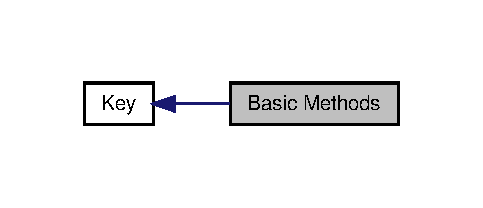
\includegraphics[width=232pt]{group__key__basic}
\end{center}
\end{figure}
Key construction and initialization methods. To use them\-: 
\begin{DoxyCode}
\textcolor{preprocessor}{#include <kdb.h>}
\end{DoxyCode}


Key properties are\-:
\begin{DoxyItemize}
\item \hyperlink{group__keyname}{Key name }
\item \hyperlink{group__keyvalue}{Key value }
\item \hyperlink{group__keyvalue_gafb89735689929ff717cc9f2d0d0b46a2}{Key comment }
\item \hyperlink{group__keyname_ga35922a017bee8b4bcb493bbdfad9d6f5}{Key owner }
\item \hyperlink{group__keymeta}{U\-I\-D, G\-I\-D and filesystem-\/like mode permissions }
\item \hyperlink{group__keymeta}{Mode, change and modification times }
\end{DoxyItemize}

Described here the methods to allocate and free the key. 
\hypertarget{group__keymeta}{}\doxysection{Meta Info Manipulation Methods}
\label{group__keymeta}\index{Meta Info Manipulation Methods@{Meta Info Manipulation Methods}}


Methods to do various operations on Key metadata.  


Collaboration diagram for Meta Info Manipulation Methods\+:
\nopagebreak
\begin{figure}[H]
\begin{center}
\leavevmode
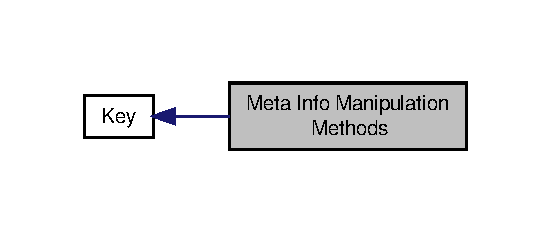
\includegraphics[width=281pt]{group__keymeta}
\end{center}
\end{figure}
\doxysubsection*{Functions}
\begin{DoxyCompactItemize}
\item 
int \mbox{\hyperlink{group__keymeta_ga5dbb669802eea27e106ee3a5e39717a9}{key\+Rewind\+Meta}} (Key $\ast$key)
\begin{DoxyCompactList}\small\item\em Rewind the internal iterator to the first entry in metadata keyset. \end{DoxyCompactList}\item 
const Key $\ast$ \mbox{\hyperlink{group__keymeta_ga4c88342f580a4291455a801af71ce048}{key\+Next\+Meta}} (Key $\ast$key)
\begin{DoxyCompactList}\small\item\em Get the next metadata entry of a Key. \end{DoxyCompactList}\item 
const Key $\ast$ \mbox{\hyperlink{group__keymeta_ga74a273f529030f4947df52e14fdd2869}{key\+Current\+Meta}} (const Key $\ast$key)
\begin{DoxyCompactList}\small\item\em Returns the metadata Key at the internal iterator\textquotesingle{}s current position. \end{DoxyCompactList}\item 
int \mbox{\hyperlink{group__keymeta_ga9a22b992478e613c8788bd460b4a1f0c}{key\+Copy\+Meta}} (Key $\ast$dest, const Key $\ast$source, const char $\ast$meta\+Name)
\begin{DoxyCompactList}\small\item\em Do a shallow copy of metadata with name {\ttfamily meta\+Name} from source to dest. \end{DoxyCompactList}\item 
int \mbox{\hyperlink{group__keymeta_ga8e63720a65610a29597494d0671f9401}{key\+Copy\+All\+Meta}} (Key $\ast$dest, const Key $\ast$source)
\begin{DoxyCompactList}\small\item\em Do a shallow copy of all metadata from source to dest. \end{DoxyCompactList}\item 
const Key $\ast$ \mbox{\hyperlink{group__keymeta_ga9ed3875495ddb3d8a8d29158a60a147c}{key\+Get\+Meta}} (const Key $\ast$key, const char $\ast$meta\+Name)
\begin{DoxyCompactList}\small\item\em Returns the Key for a metadata entry with name {\ttfamily meta\+Name}. \end{DoxyCompactList}\item 
ssize\+\_\+t \mbox{\hyperlink{group__keymeta_gae1f15546b234ffb6007d8a31178652b9}{key\+Set\+Meta}} (Key $\ast$key, const char $\ast$meta\+Name, const char $\ast$new\+Meta\+String)
\begin{DoxyCompactList}\small\item\em Set a new metadata Key. \end{DoxyCompactList}\item 
Key\+Set $\ast$ \mbox{\hyperlink{group__keymeta_ga11706f1753e67933f7cffc5c0345cd29}{key\+Meta}} (Key $\ast$key)
\begin{DoxyCompactList}\small\item\em Returns the Key\+Set holding the given Key\textquotesingle{}s metadata. \end{DoxyCompactList}\end{DoxyCompactItemize}


\doxysubsection{Detailed Description}
Methods to do various operations on Key metadata. 

To use them\+: 
\begin{DoxyCode}{0}
\DoxyCodeLine{\textcolor{preprocessor}{\#include <kdb.h>}}

\end{DoxyCode}


Next to \mbox{\hyperlink{group__keyname}{Name (key and owner) }} and \mbox{\hyperlink{group__keyvalue}{value (data and comment) }} there is the so called meta information inside every key.

Key meta information are an unlimited number of key/value pairs strongly related to a key. It main purpose is to give keys special semantics, so that plugins can treat them differently.

Metakey, as opposed to Key, deliberately has following limitations\+:
\begin{DoxyItemize}
\item no null values
\item no binary data
\item no modification of references (COW)
\item no guarantee of ordering
\end{DoxyItemize}\hypertarget{group__keymeta_autotoc_md0}{}\doxysubsubsection{Examples for metadata}\label{group__keymeta_autotoc_md0}
File system information (see stat(2) for more information)\+:
\begin{DoxyItemize}
\item uid\+: the user id (positive number)
\item gid\+: the group id (positive number)
\item mode\+: filesystem-\/like mode permissions (positive octal number)
\item atime\+: When was the key accessed the last time.
\item mtime\+: When was the key modified the last time.
\item ctime\+: When the uid, gid or mode of a key changes. (times are represented through a positive number as unix timestamp)
\end{DoxyItemize}

The comment can contain userdata which directly belong to that key. The name of the meta information is \char`\"{}comment\char`\"{} for a general purpose comment about the key. Multi-\/\+Language comments are also supported by appending \mbox{[}LANG\mbox{]} to the name.

Validators are regular expressions which are tested against the key value. The metakey \char`\"{}validator\char`\"{} can hold a regular expression which will be matched against.

Types can be expressed with the meta information \char`\"{}type\char`\"{}.

The relevance of the key can be tagged with a value from -\/20 to 20. Negative numbers are the more important and must be present in order to start the program.

A version of a key may be stored with \char`\"{}version\char`\"{}. Its format is full.\+major.\+minor where all of these are integers.

The order inside a persistent storage can be described with the tag \char`\"{}order\char`\"{} which contains a positive number.

The metakey \char`\"{}app\char`\"{} describes to which application a key belongs. It can be used to remove keys from an application no longer installed.

The metakey \char`\"{}path\char`\"{} describes where the key is physically stored.

The \char`\"{}owner\char`\"{} is the user that owns the key. It only works for the user\+:/ hierarchy. It rather says where the key is stored and says nothing about the filesystem properties. 

\doxysubsection{Function Documentation}
\mbox{\Hypertarget{group__keymeta_ga8e63720a65610a29597494d0671f9401}\label{group__keymeta_ga8e63720a65610a29597494d0671f9401}} 
\index{Meta Info Manipulation Methods@{Meta Info Manipulation Methods}!keyCopyAllMeta@{keyCopyAllMeta}}
\index{keyCopyAllMeta@{keyCopyAllMeta}!Meta Info Manipulation Methods@{Meta Info Manipulation Methods}}
\doxysubsubsection{\texorpdfstring{keyCopyAllMeta()}{keyCopyAllMeta()}}
{\footnotesize\ttfamily int key\+Copy\+All\+Meta (\begin{DoxyParamCaption}\item[{Key $\ast$}]{dest,  }\item[{const Key $\ast$}]{source }\end{DoxyParamCaption})}



Do a shallow copy of all metadata from source to dest. 

The key dest will additionally have all metadata the source had. Metadata not present in source will not be changed. Metadata which was present in source and dest will be overwritten. If the {\ttfamily dest} Key is read-\/only it will not be changed.

For example the metadata type is copied into the Key k\+:


\begin{DoxyCodeInclude}{0}
\DoxyCodeLine{\textcolor{keywordtype}{void} l (Key * k)}
\DoxyCodeLine{\{}
\DoxyCodeLine{        \textcolor{comment}{// receive copy}}
\DoxyCodeLine{        \mbox{\hyperlink{group__keymeta_ga8e63720a65610a29597494d0671f9401}{keyCopyAllMeta}} (k, copy);}
\DoxyCodeLine{        \textcolor{comment}{// the caller will see the changed key k}}
\DoxyCodeLine{        \textcolor{comment}{// with all the metadata from copy}}
\DoxyCodeLine{\}}

\end{DoxyCodeInclude}
 The main purpose of this function is for plugins or applications which want to add the same metadata to n keys. When you do that with \mbox{\hyperlink{group__keymeta_gae1f15546b234ffb6007d8a31178652b9}{key\+Set\+Meta()}} it will take n times the memory for the key. This can be considerable amount of memory for many keys with some metadata for each.

To avoid that problem you can use \mbox{\hyperlink{group__keymeta_ga8e63720a65610a29597494d0671f9401}{key\+Copy\+All\+Meta()}} or \mbox{\hyperlink{group__keymeta_ga9a22b992478e613c8788bd460b4a1f0c}{key\+Copy\+Meta()}}\+:


\begin{DoxyCodeInclude}{0}
\DoxyCodeLine{\textcolor{keywordtype}{void} o (KeySet * ks)}
\DoxyCodeLine{\{}
\DoxyCodeLine{        Key * current;}
\DoxyCodeLine{        Key * shared = \mbox{\hyperlink{group__key_gad23c65b44bf48d773759e1f9a4d43b89}{keyNew}} (\textcolor{stringliteral}{"{}/"{}}, \mbox{\hyperlink{group__key_gga9b703ca49f48b482def322b77d3e6bc8aa8adb6fcb92dec58fb19410eacfdd403}{KEY\_END}});}
\DoxyCodeLine{        \mbox{\hyperlink{group__keymeta_gae1f15546b234ffb6007d8a31178652b9}{keySetMeta}} (shared, \textcolor{stringliteral}{"{}shared1"{}}, \textcolor{stringliteral}{"{}this metadata should be shared among many keys"{}});}
\DoxyCodeLine{        \mbox{\hyperlink{group__keymeta_gae1f15546b234ffb6007d8a31178652b9}{keySetMeta}} (shared, \textcolor{stringliteral}{"{}shared2"{}}, \textcolor{stringliteral}{"{}this metadata should be shared among many keys also"{}});}
\DoxyCodeLine{        \mbox{\hyperlink{group__keymeta_gae1f15546b234ffb6007d8a31178652b9}{keySetMeta}} (shared, \textcolor{stringliteral}{"{}shared3"{}}, \textcolor{stringliteral}{"{}this metadata should be shared among many keys too"{}});}
\DoxyCodeLine{}
\DoxyCodeLine{        \mbox{\hyperlink{group__keyset_gabe793ff51f1728e3429c84a8a9086b70}{ksRewind}} (ks);}
\DoxyCodeLine{        \textcolor{keywordflow}{while} ((current = \mbox{\hyperlink{group__keyset_ga317321c9065b5a4b3e33fe1c399bcec9}{ksNext}} (ks)) != 0)}
\DoxyCodeLine{        \{}
\DoxyCodeLine{                \textcolor{keywordflow}{if} (needsSharedData (current)) \mbox{\hyperlink{group__keymeta_ga8e63720a65610a29597494d0671f9401}{keyCopyAllMeta}} (current, shared);}
\DoxyCodeLine{        \}}
\DoxyCodeLine{}
\DoxyCodeLine{        \mbox{\hyperlink{group__key_ga3df95bbc2494e3e6703ece5639be5bb1}{keyDel}} (shared);}
\DoxyCodeLine{\}}

\end{DoxyCodeInclude}
 \begin{DoxyPrecond}{Precondition}
{\ttfamily dest\textquotesingle{}s} metadata is not read-\/only 
\end{DoxyPrecond}
\begin{DoxyPostcond}{Postcondition}
for every meta\+Name present in source\+: key\+Get\+Meta(source, meta\+Name) == key\+Get\+Meta(dest, meta\+Name)
\end{DoxyPostcond}

\begin{DoxyParams}{Parameters}
{\em dest} & the destination where the metadata should be copied too \\
\hline
{\em source} & the key where the metadata should be copied from\\
\hline
\end{DoxyParams}

\begin{DoxyRetVals}{Return values}
{\em 1} & if metadata was successfully copied \\
\hline
{\em 0} & if source did not have any metadata \\
\hline
{\em -\/1} & on null pointer of dest or source \\
\hline
{\em -\/1} & on memory problems\\
\hline
\end{DoxyRetVals}
\begin{DoxySince}{Since}
1.\+0.\+0
\end{DoxySince}
\begin{DoxySeeAlso}{See also}
\mbox{\hyperlink{group__keymeta_ga9a22b992478e613c8788bd460b4a1f0c}{key\+Copy\+Meta()}} for copying one metadata Key from {\ttfamily dest} to {\ttfamily source} 
\end{DoxySeeAlso}
\mbox{\Hypertarget{group__keymeta_ga9a22b992478e613c8788bd460b4a1f0c}\label{group__keymeta_ga9a22b992478e613c8788bd460b4a1f0c}} 
\index{Meta Info Manipulation Methods@{Meta Info Manipulation Methods}!keyCopyMeta@{keyCopyMeta}}
\index{keyCopyMeta@{keyCopyMeta}!Meta Info Manipulation Methods@{Meta Info Manipulation Methods}}
\doxysubsubsection{\texorpdfstring{keyCopyMeta()}{keyCopyMeta()}}
{\footnotesize\ttfamily int key\+Copy\+Meta (\begin{DoxyParamCaption}\item[{Key $\ast$}]{dest,  }\item[{const Key $\ast$}]{source,  }\item[{const char $\ast$}]{meta\+Name }\end{DoxyParamCaption})}



Do a shallow copy of metadata with name {\ttfamily meta\+Name} from source to dest. 

Afterwards {\ttfamily source} and {\ttfamily dest} will have the same metadata referred with {\ttfamily meta\+Name}. If the Key with name {\ttfamily meta\+Name} doesn\textquotesingle{}t exist in {\ttfamily source} -\/ it gets deleted in {\ttfamily dest}.

For example the metadata type is copied into the Key k.


\begin{DoxyCode}{0}
\DoxyCodeLine{\textcolor{keywordtype}{void} l(Key *k)}
\DoxyCodeLine{\{}
\DoxyCodeLine{        \textcolor{comment}{// receive c}}
\DoxyCodeLine{        \mbox{\hyperlink{group__keymeta_ga9a22b992478e613c8788bd460b4a1f0c}{keyCopyMeta}}(k, c, \textcolor{stringliteral}{"{}type"{}});}
\DoxyCodeLine{        \textcolor{comment}{// the caller will see the changed key k}}
\DoxyCodeLine{        \textcolor{comment}{// with the metadata "{}type"{} from c}}
\DoxyCodeLine{\}}

\end{DoxyCode}


The main purpose of this function is for plugins or applications, which want to add the same metadata to n keys. When you do that \mbox{\hyperlink{group__keymeta_gae1f15546b234ffb6007d8a31178652b9}{key\+Set\+Meta()}} will take n times the memory for the key. This can be a considerable amount of memory for many keys with some metadata for each.

To avoid that problem you can use \mbox{\hyperlink{group__keymeta_ga8e63720a65610a29597494d0671f9401}{key\+Copy\+All\+Meta()}} or \mbox{\hyperlink{group__keymeta_ga9a22b992478e613c8788bd460b4a1f0c}{key\+Copy\+Meta()}}.


\begin{DoxyCode}{0}
\DoxyCodeLine{\textcolor{keywordtype}{void} o(KeySet *ks)}
\DoxyCodeLine{\{}
\DoxyCodeLine{        Key *current;}
\DoxyCodeLine{        Key *shared = \mbox{\hyperlink{group__key_gad23c65b44bf48d773759e1f9a4d43b89}{keyNew}} (\textcolor{stringliteral}{"{}/"{}}, \mbox{\hyperlink{group__key_gga9b703ca49f48b482def322b77d3e6bc8aa8adb6fcb92dec58fb19410eacfdd403}{KEY\_END}});}
\DoxyCodeLine{        \mbox{\hyperlink{group__keymeta_gae1f15546b234ffb6007d8a31178652b9}{keySetMeta}}(shared, \textcolor{stringliteral}{"{}shared"{}}, \textcolor{stringliteral}{"{}this metadata should be shared among many keys"{}});}
\DoxyCodeLine{}
\DoxyCodeLine{        \mbox{\hyperlink{group__keyset_gabe793ff51f1728e3429c84a8a9086b70}{ksRewind}}(ks);}
\DoxyCodeLine{        \textcolor{keywordflow}{while} ((current = \mbox{\hyperlink{group__keyset_ga317321c9065b5a4b3e33fe1c399bcec9}{ksNext}}(ks)) != 0)}
\DoxyCodeLine{        \{}
\DoxyCodeLine{                \textcolor{keywordflow}{if} (needs\_shared\_data(current)) \mbox{\hyperlink{group__keymeta_ga9a22b992478e613c8788bd460b4a1f0c}{keyCopyMeta}}(current, shared, \textcolor{stringliteral}{"{}shared"{}});}
\DoxyCodeLine{        \}}
\DoxyCodeLine{\}}

\end{DoxyCode}


\begin{DoxyPrecond}{Precondition}
{\ttfamily dest\textquotesingle{}s} metadata is not read-\/only 
\end{DoxyPrecond}
\begin{DoxyPostcond}{Postcondition}
key\+Get\+Meta(source, meta\+Name) == key\+Get\+Meta(dest, meta\+Name)
\end{DoxyPostcond}

\begin{DoxyParams}{Parameters}
{\em dest} & the destination where the metadata should be copied to \\
\hline
{\em source} & the key where the metadata should be copied from \\
\hline
{\em meta\+Name} & the name of the metadata Key which should be copied\\
\hline
\end{DoxyParams}

\begin{DoxyRetVals}{Return values}
{\em 1} & if was successfully copied \\
\hline
{\em 0} & if the metadata in dest was removed too \\
\hline
{\em -\/1} & on null pointers (source or dest) \\
\hline
{\em -\/1} & on memory problems \\
\hline
{\em -\/1} & if metadata is read-\/only\\
\hline
\end{DoxyRetVals}
\begin{DoxySince}{Since}
1.\+0.\+0
\end{DoxySince}
\begin{DoxySeeAlso}{See also}
\mbox{\hyperlink{group__keymeta_ga8e63720a65610a29597494d0671f9401}{key\+Copy\+All\+Meta()}} copies all metadata from {\ttfamily dest} to {\ttfamily src} 
\end{DoxySeeAlso}
\mbox{\Hypertarget{group__keymeta_ga74a273f529030f4947df52e14fdd2869}\label{group__keymeta_ga74a273f529030f4947df52e14fdd2869}} 
\index{Meta Info Manipulation Methods@{Meta Info Manipulation Methods}!keyCurrentMeta@{keyCurrentMeta}}
\index{keyCurrentMeta@{keyCurrentMeta}!Meta Info Manipulation Methods@{Meta Info Manipulation Methods}}
\doxysubsubsection{\texorpdfstring{keyCurrentMeta()}{keyCurrentMeta()}}
{\footnotesize\ttfamily const Key$\ast$ key\+Current\+Meta (\begin{DoxyParamCaption}\item[{const Key $\ast$}]{key }\end{DoxyParamCaption})}



Returns the metadata Key at the internal iterator\textquotesingle{}s current position. 

The returned pointer is NULL if the end has been reached or after calling \mbox{\hyperlink{group__keyset_gabe793ff51f1728e3429c84a8a9086b70}{ks\+Rewind()}}.

\begin{DoxyNote}{Note}
You must not delete or change the returned key, use \mbox{\hyperlink{group__keymeta_gae1f15546b234ffb6007d8a31178652b9}{key\+Set\+Meta()}} if you want to delete or change it.
\end{DoxyNote}

\begin{DoxyParams}{Parameters}
{\em key} & Key to get the current metadata from\\
\hline
\end{DoxyParams}
\begin{DoxyReturn}{Returns}
a buffer to the value pointed by {\ttfamily key\textquotesingle{}s} cursor 
\end{DoxyReturn}

\begin{DoxyRetVals}{Return values}
{\em 0} & on NULL pointer\\
\hline
\end{DoxyRetVals}
\begin{DoxySince}{Since}
1.\+0.\+0
\end{DoxySince}
\begin{DoxySeeAlso}{See also}
\mbox{\hyperlink{group__keymeta_ga4c88342f580a4291455a801af71ce048}{key\+Next\+Meta()}} for getting the next value 

\mbox{\hyperlink{group__keymeta_ga5dbb669802eea27e106ee3a5e39717a9}{key\+Rewind\+Meta()}} for rewinding the internal iterator 

\mbox{\hyperlink{group__keyset_ga4287b9416912c5f2ab9c195cb74fb094}{ks\+Current()}} Key\+Sets\textquotesingle{}s equivalent function for getting the current Key 
\end{DoxySeeAlso}
\mbox{\Hypertarget{group__keymeta_ga9ed3875495ddb3d8a8d29158a60a147c}\label{group__keymeta_ga9ed3875495ddb3d8a8d29158a60a147c}} 
\index{Meta Info Manipulation Methods@{Meta Info Manipulation Methods}!keyGetMeta@{keyGetMeta}}
\index{keyGetMeta@{keyGetMeta}!Meta Info Manipulation Methods@{Meta Info Manipulation Methods}}
\doxysubsubsection{\texorpdfstring{keyGetMeta()}{keyGetMeta()}}
{\footnotesize\ttfamily const Key$\ast$ key\+Get\+Meta (\begin{DoxyParamCaption}\item[{const Key $\ast$}]{key,  }\item[{const char $\ast$}]{meta\+Name }\end{DoxyParamCaption})}



Returns the Key for a metadata entry with name {\ttfamily meta\+Name}. 

You are not allowed to modify the resulting key.

If {\ttfamily meta\+Name} does not start with \textquotesingle{}meta\+:/\textquotesingle{}, it will be prefixed with \textquotesingle{}meta\+:/\textquotesingle{}.


\begin{DoxyCode}{0}
\DoxyCodeLine{Key metaData = \mbox{\hyperlink{group__keymeta_ga9ed3875495ddb3d8a8d29158a60a147c}{keyGetMeta}}(k, \textcolor{stringliteral}{"{}type"{}})}
\DoxyCodeLine{\textcolor{comment}{// keyType == "{}boolean"{}}}
\DoxyCodeLine{char keyType[] = \mbox{\hyperlink{group__keyvalue_ga6f29609c5da53c6dc26a98678d5752af}{keyValue}}(metaData)}

\end{DoxyCode}


\begin{DoxyNote}{Note}
You must not delete or change the returned key, use \mbox{\hyperlink{group__keymeta_gae1f15546b234ffb6007d8a31178652b9}{key\+Set\+Meta()}} if you want to delete or change it.
\end{DoxyNote}
\begin{DoxyPrecond}{Precondition}
{\ttfamily key} contains metadata 

{\ttfamily meta\+Name} is prefixed with \char`\"{}meta\+:/\char`\"{}
\end{DoxyPrecond}

\begin{DoxyParams}{Parameters}
{\em key} & the Key from which to get metadata \\
\hline
{\em meta\+Name} & the name of the meta information you want the Key from.\\
\hline
\end{DoxyParams}
\begin{DoxyReturn}{Returns}
value of meta-\/information if meta-\/information is found 
\end{DoxyReturn}

\begin{DoxyRetVals}{Return values}
{\em 0} & if key or meta\+Name is NULL \\
\hline
{\em 0} & if no such meta\+Name is found\\
\hline
\end{DoxyRetVals}
\begin{DoxySince}{Since}
1.\+0.\+0
\end{DoxySince}
\begin{DoxySeeAlso}{See also}
\mbox{\hyperlink{group__keymeta_gae1f15546b234ffb6007d8a31178652b9}{key\+Set\+Meta()}} for setting metadata 

\mbox{\hyperlink{group__keymeta_ga11706f1753e67933f7cffc5c0345cd29}{key\+Meta()}} for getting the Key\+Set containing metadata 
\end{DoxySeeAlso}
\mbox{\Hypertarget{group__keymeta_ga11706f1753e67933f7cffc5c0345cd29}\label{group__keymeta_ga11706f1753e67933f7cffc5c0345cd29}} 
\index{Meta Info Manipulation Methods@{Meta Info Manipulation Methods}!keyMeta@{keyMeta}}
\index{keyMeta@{keyMeta}!Meta Info Manipulation Methods@{Meta Info Manipulation Methods}}
\doxysubsubsection{\texorpdfstring{keyMeta()}{keyMeta()}}
{\footnotesize\ttfamily Key\+Set$\ast$ key\+Meta (\begin{DoxyParamCaption}\item[{Key $\ast$}]{key }\end{DoxyParamCaption})}



Returns the Key\+Set holding the given Key\textquotesingle{}s metadata. 

Use \mbox{\hyperlink{group__keymeta_gae1f15546b234ffb6007d8a31178652b9}{key\+Set\+Meta()}} to populate the metadata Key\+Set of a Key.


\begin{DoxyCodeInclude}{0}
\DoxyCodeLine{        Key * key = \mbox{\hyperlink{group__key_gad23c65b44bf48d773759e1f9a4d43b89}{keyNew}} (\textcolor{stringliteral}{"{}user:/test/key"{}}, \mbox{\hyperlink{group__key_gga9b703ca49f48b482def322b77d3e6bc8aa8adb6fcb92dec58fb19410eacfdd403}{KEY\_END}});}
\DoxyCodeLine{}
\DoxyCodeLine{        \mbox{\hyperlink{group__keymeta_gae1f15546b234ffb6007d8a31178652b9}{keySetMeta}} (key, \textcolor{stringliteral}{"{}meta1"{}}, \textcolor{stringliteral}{"{}value1"{}});}
\DoxyCodeLine{        \mbox{\hyperlink{group__keymeta_gae1f15546b234ffb6007d8a31178652b9}{keySetMeta}} (key, \textcolor{stringliteral}{"{}meta2"{}}, \textcolor{stringliteral}{"{}value2"{}});}

\end{DoxyCodeInclude}
 Iterate the returned metadata Key\+Set like any other Key\+Set.


\begin{DoxyCodeInclude}{0}
\DoxyCodeLine{        Key * cur;}
\DoxyCodeLine{        \mbox{\hyperlink{group__keyset_gabe793ff51f1728e3429c84a8a9086b70}{ksRewind}} (\mbox{\hyperlink{group__keymeta_ga11706f1753e67933f7cffc5c0345cd29}{keyMeta}} (key));}
\DoxyCodeLine{        \textcolor{keywordflow}{while} ((cur = \mbox{\hyperlink{group__keyset_ga317321c9065b5a4b3e33fe1c399bcec9}{ksNext}} (\mbox{\hyperlink{group__keymeta_ga11706f1753e67933f7cffc5c0345cd29}{keyMeta}} (key))) != NULL)}
\DoxyCodeLine{        \{}
\DoxyCodeLine{                printf (\textcolor{stringliteral}{"{}meta name: \%s, meta value: \%s\(\backslash\)n"{}}, \mbox{\hyperlink{group__keyname_ga8e805c726a60da921d3736cda7813513}{keyName}} (cur), \mbox{\hyperlink{group__keyvalue_ga880936f2481d28e6e2acbe7486a21d05}{keyString}} (cur));}
\DoxyCodeLine{        \}}

\end{DoxyCodeInclude}
 Use \mbox{\hyperlink{group__keyset_ga60f1ddcf23272f2b29b90e92ebe9b56f}{ks\+Lookup()}} or \mbox{\hyperlink{group__keymeta_ga9ed3875495ddb3d8a8d29158a60a147c}{key\+Get\+Meta()}} to retrieve a single value for a given Key.


\begin{DoxyCodeInclude}{0}
\DoxyCodeLine{        Key * lookupKey = \mbox{\hyperlink{group__keyset_gad65d2cdcbb5381194a1688e169af8a83}{ksLookupByName}} (\mbox{\hyperlink{group__keymeta_ga11706f1753e67933f7cffc5c0345cd29}{keyMeta}} (key), \textcolor{stringliteral}{"{}meta2"{}}, 0);}
\DoxyCodeLine{        printf (\textcolor{stringliteral}{"{}meta name: \%s, meta value: \%s\(\backslash\)n"{}}, \mbox{\hyperlink{group__keyname_ga8e805c726a60da921d3736cda7813513}{keyName}} (lookupKey), \mbox{\hyperlink{group__keyvalue_ga880936f2481d28e6e2acbe7486a21d05}{keyString}} (lookupKey));}
\DoxyCodeLine{        \mbox{\hyperlink{group__key_ga3df95bbc2494e3e6703ece5639be5bb1}{keyDel}} (key);}

\end{DoxyCodeInclude}
 \begin{DoxyNote}{Note}
You are not allowed to modify the name of Key\+Set\textquotesingle{}s Keys or delete them. 

You must not delete the returned Key\+Set. 

Adding a key with metadata to the Key\+Set is an error.
\end{DoxyNote}
\begin{DoxyPostcond}{Postcondition}
for the returned Key\+Set ks\+: key\+Get\+Meta(key, meta\+Name) == ks\+Lookup\+By\+Name(ks, meta\+Name) 

{\ttfamily key} contains a Key\+Set for the metadata
\end{DoxyPostcond}

\begin{DoxyParams}{Parameters}
{\em key} & the Key from which to get the metadata Key\+Set\\
\hline
\end{DoxyParams}
\begin{DoxyReturn}{Returns}
the Key\+Set holding the metadata 
\end{DoxyReturn}

\begin{DoxyRetVals}{Return values}
{\em 0} & if the Key is 0 \\
\hline
{\em 0} & if the Key has no metadata\\
\hline
\end{DoxyRetVals}
\begin{DoxySince}{Since}
1.\+0.\+0
\end{DoxySince}
\begin{DoxySeeAlso}{See also}
\mbox{\hyperlink{group__keymeta_gae1f15546b234ffb6007d8a31178652b9}{key\+Set\+Meta()}} for setting a metadata Key 

\mbox{\hyperlink{group__keymeta_ga9ed3875495ddb3d8a8d29158a60a147c}{key\+Get\+Meta()}} for getting a metadata Key 
\end{DoxySeeAlso}
\mbox{\Hypertarget{group__keymeta_ga4c88342f580a4291455a801af71ce048}\label{group__keymeta_ga4c88342f580a4291455a801af71ce048}} 
\index{Meta Info Manipulation Methods@{Meta Info Manipulation Methods}!keyNextMeta@{keyNextMeta}}
\index{keyNextMeta@{keyNextMeta}!Meta Info Manipulation Methods@{Meta Info Manipulation Methods}}
\doxysubsubsection{\texorpdfstring{keyNextMeta()}{keyNextMeta()}}
{\footnotesize\ttfamily const Key$\ast$ key\+Next\+Meta (\begin{DoxyParamCaption}\item[{Key $\ast$}]{key }\end{DoxyParamCaption})}



Get the next metadata entry of a Key. 

Keys have an internal cursor that can be reset with \mbox{\hyperlink{group__keymeta_ga5dbb669802eea27e106ee3a5e39717a9}{key\+Rewind\+Meta()}}. Every time \mbox{\hyperlink{group__keymeta_ga4c88342f580a4291455a801af71ce048}{key\+Next\+Meta()}} is called the cursor is incremented and the new current Name of Meta Information is returned.

You\textquotesingle{}ll get a NULL pointer if the metadata after the end of the Key was reached. On subsequent calls of \mbox{\hyperlink{group__keymeta_ga4c88342f580a4291455a801af71ce048}{key\+Next\+Meta()}} it will still return the NULL pointer.

The {\ttfamily key} internal cursor will be changed, so it is not const.

\begin{DoxyNote}{Note}
That the resulting key is guaranteed to have a value, because meta information has no binary or null pointer semantics.

You must not delete or change the returned key, use \mbox{\hyperlink{group__keymeta_gae1f15546b234ffb6007d8a31178652b9}{key\+Set\+Meta()}} if you want to delete or change it.
\end{DoxyNote}

\begin{DoxyParams}{Parameters}
{\em key} & the Key object to work with\\
\hline
\end{DoxyParams}
\begin{DoxyReturn}{Returns}
a key containing metadata 
\end{DoxyReturn}

\begin{DoxyRetVals}{Return values}
{\em 0} & when the last Key has been reached \\
\hline
{\em 0} & when Key is a NULL pointer\\
\hline
\end{DoxyRetVals}
\begin{DoxySince}{Since}
1.\+0.\+0
\end{DoxySince}
\begin{DoxySeeAlso}{See also}
\mbox{\hyperlink{group__keyset_ga317321c9065b5a4b3e33fe1c399bcec9}{ks\+Next()}} for pedant in iterator interface of Key\+Set 

\mbox{\hyperlink{group__keymeta_ga5dbb669802eea27e106ee3a5e39717a9}{key\+Rewind\+Meta()}} for rewinding the internal iterator 

\mbox{\hyperlink{group__keymeta_ga74a273f529030f4947df52e14fdd2869}{key\+Current\+Meta()}} for getting the current metadata Key 
\end{DoxySeeAlso}
\mbox{\Hypertarget{group__keymeta_ga5dbb669802eea27e106ee3a5e39717a9}\label{group__keymeta_ga5dbb669802eea27e106ee3a5e39717a9}} 
\index{Meta Info Manipulation Methods@{Meta Info Manipulation Methods}!keyRewindMeta@{keyRewindMeta}}
\index{keyRewindMeta@{keyRewindMeta}!Meta Info Manipulation Methods@{Meta Info Manipulation Methods}}
\doxysubsubsection{\texorpdfstring{keyRewindMeta()}{keyRewindMeta()}}
{\footnotesize\ttfamily int key\+Rewind\+Meta (\begin{DoxyParamCaption}\item[{Key $\ast$}]{key }\end{DoxyParamCaption})}



Rewind the internal iterator to the first entry in metadata keyset. 

Use this function to set the cursor to the beginning of the Key Meta Infos. \mbox{\hyperlink{group__keymeta_ga74a273f529030f4947df52e14fdd2869}{key\+Current\+Meta()}} will always return NULL after rewinding, so you need to call \mbox{\hyperlink{group__keymeta_ga4c88342f580a4291455a801af71ce048}{key\+Next\+Meta()}} first.


\begin{DoxyCode}{0}
\DoxyCodeLine{Key *key;}
\DoxyCodeLine{\textcolor{keyword}{const} Key *meta;}
\DoxyCodeLine{}
\DoxyCodeLine{\mbox{\hyperlink{group__keymeta_ga5dbb669802eea27e106ee3a5e39717a9}{keyRewindMeta}} (key);}
\DoxyCodeLine{\textcolor{keywordflow}{while} ((meta = \mbox{\hyperlink{group__keymeta_ga4c88342f580a4291455a801af71ce048}{keyNextMeta}} (key))!=0)}
\DoxyCodeLine{\{}
\DoxyCodeLine{        printf (\textcolor{stringliteral}{"{}name: \%s, value: \%s"{}}, \mbox{\hyperlink{group__keyname_ga8e805c726a60da921d3736cda7813513}{keyName}}(meta), \mbox{\hyperlink{group__keyvalue_ga880936f2481d28e6e2acbe7486a21d05}{keyString}}(meta));}
\DoxyCodeLine{\}}

\end{DoxyCode}



\begin{DoxyParams}{Parameters}
{\em key} & Key whose internal iterator should be rewinded\\
\hline
\end{DoxyParams}

\begin{DoxyRetVals}{Return values}
{\em 0} & on success \\
\hline
{\em 0} & if there is no metadata for that key (\mbox{\hyperlink{group__keymeta_ga4c88342f580a4291455a801af71ce048}{key\+Next\+Meta()}} will always return 0 in that case) \\
\hline
{\em -\/1} & on NULL pointer\\
\hline
\end{DoxyRetVals}
\begin{DoxySince}{Since}
1.\+0.\+0
\end{DoxySince}
\begin{DoxySeeAlso}{See also}
\mbox{\hyperlink{group__keymeta_ga4c88342f580a4291455a801af71ce048}{key\+Next\+Meta()}}, \mbox{\hyperlink{group__keymeta_ga74a273f529030f4947df52e14fdd2869}{key\+Current\+Meta()}} for iterating after rewinding 

\mbox{\hyperlink{group__keyset_gabe793ff51f1728e3429c84a8a9086b70}{ks\+Rewind()}} Key\+Set\textquotesingle{}s equivalent function for rewinding 
\end{DoxySeeAlso}
\mbox{\Hypertarget{group__keymeta_gae1f15546b234ffb6007d8a31178652b9}\label{group__keymeta_gae1f15546b234ffb6007d8a31178652b9}} 
\index{Meta Info Manipulation Methods@{Meta Info Manipulation Methods}!keySetMeta@{keySetMeta}}
\index{keySetMeta@{keySetMeta}!Meta Info Manipulation Methods@{Meta Info Manipulation Methods}}
\doxysubsubsection{\texorpdfstring{keySetMeta()}{keySetMeta()}}
{\footnotesize\ttfamily ssize\+\_\+t key\+Set\+Meta (\begin{DoxyParamCaption}\item[{Key $\ast$}]{key,  }\item[{const char $\ast$}]{meta\+Name,  }\item[{const char $\ast$}]{new\+Meta\+String }\end{DoxyParamCaption})}



Set a new metadata Key. 

Will set a new metadata pair with name {\ttfamily meta\+Name} and value {\ttfamily new\+Meta\+String}.

Will add a new metadata Key, if {\ttfamily meta\+Name} was unused until now.

It will modify an existing Pair of metadata if {\ttfamily meta\+Name} was already present.

It will remove a metadata Key if {\ttfamily new\+Meta\+String} is 0.

If {\ttfamily meta\+Name} does not start with \textquotesingle{}meta\+:/\textquotesingle{}, it will be prefixed with \textquotesingle{}meta\+:/\textquotesingle{}.

\begin{DoxyPrecond}{Precondition}
{\ttfamily meta\+Name} is prefixed with \char`\"{}meta\+:/\char`\"{} 

{\ttfamily key\textquotesingle{}s} metadata is not read-\/only 
\end{DoxyPrecond}
\begin{DoxyPostcond}{Postcondition}
The value in {\ttfamily key\textquotesingle{}s} metadata Keyset for {\ttfamily meta\+Name} is {\ttfamily new\+Meta\+String} 
\end{DoxyPostcond}

\begin{DoxyParams}{Parameters}
{\em key} & Key whose metadata should be set \\
\hline
{\em meta\+Name} & name of the metadata Key that should be set \\
\hline
{\em new\+Meta\+String} & new value for the metadata Key\\
\hline
\end{DoxyParams}
\begin{DoxyReturn}{Returns}
size ($>$0) of {\ttfamily new\+Meta\+String} if metadata has been successfully added 
\end{DoxyReturn}

\begin{DoxyRetVals}{Return values}
{\em 0} & if the meta-\/information for meta\+Name was removed \\
\hline
{\em -\/1} & if key or meta\+Name is 0 \\
\hline
{\em -\/1} & if system is out of memory \\
\hline
{\em -\/1} & if {\ttfamily meta\+Name} is not a valid metadata name\\
\hline
\end{DoxyRetVals}
\begin{DoxySince}{Since}
1.\+0.\+0
\end{DoxySince}
\begin{DoxySeeAlso}{See also}
\mbox{\hyperlink{group__keymeta_ga9ed3875495ddb3d8a8d29158a60a147c}{key\+Get\+Meta()}} for getting the value of a metadata Key 

\mbox{\hyperlink{group__keymeta_ga11706f1753e67933f7cffc5c0345cd29}{key\+Meta()}} for getting the Key\+Set containing metadata 
\end{DoxySeeAlso}

\hypertarget{group__keyname}{\section{Name Manipulation Methods}
\label{group__keyname}\index{Name Manipulation Methods@{Name Manipulation Methods}}
}


Methods to do various operations on Key names.  


Collaboration diagram for Name Manipulation Methods\-:
\nopagebreak
\begin{figure}[H]
\begin{center}
\leavevmode
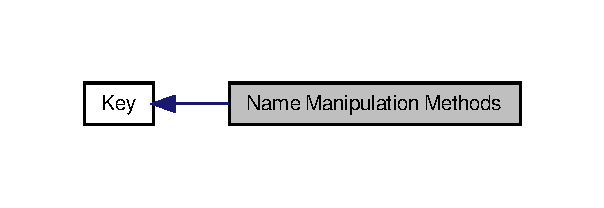
\includegraphics[width=290pt]{group__keyname}
\end{center}
\end{figure}
\subsection*{Enumerations}
\begin{DoxyCompactItemize}
\item 
enum \hyperlink{group__keyname_gaec3b8d6f430ae49b91bafe8a86310a68}{elektra\-Namespace} \{ \\*
\hyperlink{group__keyname_ggaec3b8d6f430ae49b91bafe8a86310a68a3659698b0a07454ca8055ab693e8efd1}{K\-E\-Y\-\_\-\-N\-S\-\_\-\-N\-O\-N\-E} =0, 
\hyperlink{group__keyname_ggaec3b8d6f430ae49b91bafe8a86310a68a33d6c53529b4e6921d0b1d6565df2f1f}{K\-E\-Y\-\_\-\-N\-S\-\_\-\-E\-M\-P\-T\-Y} =1, 
\hyperlink{group__keyname_ggaec3b8d6f430ae49b91bafe8a86310a68ac5fbf2c3a7ae79fa2d60c48ae3e72688}{K\-E\-Y\-\_\-\-N\-S\-\_\-\-M\-E\-T\-A} =1$<$$<$1, 
\hyperlink{group__keyname_ggaec3b8d6f430ae49b91bafe8a86310a68a2c9133e3095dccbcde5ca3bb13987b5d}{K\-E\-Y\-\_\-\-N\-S\-\_\-\-C\-A\-S\-C\-A\-D\-I\-N\-G} =1$<$$<$2, 
\\*
\hyperlink{group__keyname_ggaec3b8d6f430ae49b91bafe8a86310a68a8ce23c70010e8ac8bb540b0947e03a4e}{K\-E\-Y\-\_\-\-N\-S\-\_\-\-U\-S\-E\-R} =1$<$$<$3, 
\hyperlink{group__keyname_ggaec3b8d6f430ae49b91bafe8a86310a68a61adca2f9dff47e65dfcdb492ffa7a20}{K\-E\-Y\-\_\-\-N\-S\-\_\-\-S\-Y\-S\-T\-E\-M} =1$<$$<$4
 \}
\end{DoxyCompactItemize}
\subsection*{Functions}
\begin{DoxyCompactItemize}
\item 
const char $\ast$ \hyperlink{group__keyname_ga8e805c726a60da921d3736cda7813513}{key\-Name} (const Key $\ast$key)
\item 
ssize\-\_\-t \hyperlink{group__keyname_gabdbcfa51ed8a387e47ead207affa2d2e}{key\-Get\-Name\-Size} (const Key $\ast$key)
\item 
ssize\-\_\-t \hyperlink{group__keyname_gab29a850168d9b31c9529e90cf9ab68be}{key\-Get\-Name} (const Key $\ast$key, char $\ast$returned\-Name, size\-\_\-t max\-Size)
\item 
ssize\-\_\-t \hyperlink{group__keyname_ga7699091610e7f3f43d2949514a4b35d9}{key\-Set\-Name} (Key $\ast$key, const char $\ast$new\-Name)
\item 
ssize\-\_\-t \hyperlink{group__keyname_gab65dc9d43d3ee08d5e936a20ebbddd23}{key\-Get\-Full\-Name\-Size} (const Key $\ast$key)
\item 
ssize\-\_\-t \hyperlink{group__keyname_gaaba1494a5ffc976e0e56c43f4334a23c}{key\-Get\-Full\-Name} (const Key $\ast$key, char $\ast$returned\-Name, size\-\_\-t max\-Size)
\item 
\hyperlink{group__keyname_gaec3b8d6f430ae49b91bafe8a86310a68}{elektra\-Namespace} \hyperlink{group__keyname_gafc3ca03ed10f87eb59bdc02cf2a0de8d}{key\-Get\-Namespace} (const Key $\ast$key)
\item 
const char $\ast$ \hyperlink{group__keyname_gaaff35e7ca8af5560c47e662ceb9465f5}{key\-Base\-Name} (const Key $\ast$key)
\begin{DoxyCompactList}\small\item\em Returns a pointer to the internal unescaped key name where the {\ttfamily basename} starts. \end{DoxyCompactList}\item 
ssize\-\_\-t \hyperlink{group__keyname_ga1a0b76c5d9e5367c7e72211e6c63d43a}{key\-Get\-Base\-Name\-Size} (const Key $\ast$key)
\item 
ssize\-\_\-t \hyperlink{group__keyname_ga0992d26bcfca767cb8e77053a483eb64}{key\-Get\-Base\-Name} (const Key $\ast$key, char $\ast$returned, size\-\_\-t max\-Size)
\item 
ssize\-\_\-t \hyperlink{group__keyname_gaa942091fc4bd5c2699e49ddc50829524}{key\-Add\-Base\-Name} (Key $\ast$key, const char $\ast$base\-Name)
\item 
ssize\-\_\-t \hyperlink{group__keyname_ga6e804bd453f98c28b0ff51430d1df407}{key\-Set\-Base\-Name} (Key $\ast$key, const char $\ast$base\-Name)
\item 
const char $\ast$ \hyperlink{group__keyname_gaf6485fb8599714b6bbd830cf915ffea5}{key\-Owner} (const Key $\ast$key)
\item 
ssize\-\_\-t \hyperlink{group__keyname_ga4a4561895741ba2ad10acf007c188593}{key\-Get\-Owner\-Size} (const Key $\ast$key)
\item 
ssize\-\_\-t \hyperlink{group__keyname_ga35922a017bee8b4bcb493bbdfad9d6f5}{key\-Get\-Owner} (const Key $\ast$key, char $\ast$returned\-Owner, size\-\_\-t max\-Size)
\item 
ssize\-\_\-t \hyperlink{group__keyname_ga88d6ec200ba0707b7c1b4a88133d2be4}{key\-Set\-Owner} (Key $\ast$key, const char $\ast$new\-Owner)
\end{DoxyCompactItemize}


\subsection{Detailed Description}
Methods to do various operations on Key names. To use them\-: 
\begin{DoxyCode}
\textcolor{preprocessor}{#include <kdb.h>}
\end{DoxyCode}


These functions make it easier for C programmers to work with key names.

\begin{DoxyParagraph}{Terminology of Key Names}

\begin{DoxyItemize}
\item A {\itshape key name} (see \hyperlink{group__keyname_ga7699091610e7f3f43d2949514a4b35d9}{key\-Set\-Name()} and \hyperlink{group__keyname_ga8e805c726a60da921d3736cda7813513}{key\-Name()}) defines the place of a key within the key database. To be unique, it is always absolute and canonical.
\item Key names are composed out of many {\itshape key name parts} split by a separator. These {\itshape key name parts} do not contain a unescaped separator.
\item A {\itshape key base name} (see \hyperlink{group__keyname_ga6e804bd453f98c28b0ff51430d1df407}{key\-Set\-Base\-Name()} and \hyperlink{group__keyname_gaa942091fc4bd5c2699e49ddc50829524}{key\-Add\-Base\-Name()}) is the last part of the key name.
\item A namespace denotes the place the key comes from\-:
\begin{DoxyItemize}
\item {\itshape user} keys come from user's home directories
\item {\itshape system} keys come from systems etc directories
\end{DoxyItemize}
\item A {\itshape C-\/\-String} is a null terminated sequence of characters. So \textbackslash{}0 (null-\/character) must not occur within a C-\/\-String.
\end{DoxyItemize}
\end{DoxyParagraph}
\begin{DoxyNote}{Note}
The rules are currently not formally specified and are subject of change in the next major release. So, always prefer\-:
\begin{DoxyItemize}
\item To use \hyperlink{group__keyname_ga7699091610e7f3f43d2949514a4b35d9}{key\-Set\-Name()} and key\-Add\-Name() to get the canonified version of the keyname
\item To use \hyperlink{group__keyname_ga6e804bd453f98c28b0ff51430d1df407}{key\-Set\-Base\-Name()} and \hyperlink{group__keyname_gaa942091fc4bd5c2699e49ddc50829524}{key\-Add\-Base\-Name()} to get an escaped key name part.
\item Not to escape or canonify with your own algorithms!
\item To use key\-Unescaped\-Name() and \hyperlink{group__keyname_gaaff35e7ca8af5560c47e662ceb9465f5}{key\-Base\-Name()} to have access to the key name without escape sequences (key name parts are null terminated)
\item Not to unescape the strings yourself!
\end{DoxyItemize}
\end{DoxyNote}
\begin{DoxyParagraph}{Syntax for Key Names}
Key names and key name parts have following goals\-:
\begin{DoxyItemize}
\item The C-\/\-String passed to \hyperlink{group__keyname_ga7699091610e7f3f43d2949514a4b35d9}{key\-Set\-Name()} and key\-Add\-Name() may be any C-\/\-String.
\item The {\itshape key name parts} (e.\-g. \hyperlink{group__keyname_ga6e804bd453f98c28b0ff51430d1df407}{key\-Set\-Base\-Name()}, \hyperlink{group__keyname_gaaff35e7ca8af5560c47e662ceb9465f5}{key\-Base\-Name()}) may be any C-\/\-String. Escaping is needed to achieve both goals.
\end{DoxyItemize}
\end{DoxyParagraph}
\begin{DoxyParagraph}{Semantics for Key Name Parts}

\begin{DoxyItemize}
\item \% denotes an empty key name part.
\end{DoxyItemize}
\end{DoxyParagraph}
\begin{DoxyParagraph}{Canonicalization for Key Names}

\begin{DoxyItemize}
\item / (slash) is the separator between key name parts.
\item // is shortened to /
\item trailing / (slashes) are removed
\item . (dot) and .. (dot-\/dot) is removed in an canonical key name, with following rules\-:
\begin{DoxyItemize}
\item /./ is shortened to /
\item \-\_\-/../ is shortened to \-\_\-
\end{DoxyItemize}
\end{DoxyItemize}
\end{DoxyParagraph}
\begin{DoxyParagraph}{Conventions for key names}

\begin{DoxyItemize}
\item Key name parts starting with \# are array elements. Then only \-\_\- (underscore) followed by 0-\/9 is allowed. So we have the regular expression \#\mbox{[}\-\_\-\mbox{]}$\ast$\mbox{[}0-\/9\mbox{]}+ with the further limitation that the number of \-\_\- is defined by the number of digits-\/1.
\item Key name parts starting with \-\_\- are reserved for special purposes (if you use this within a plugin you still have to make sure \-\_\- is escaped properly)
\item Key name parts starting with @ are reserved for special purposes (if you use this within a plugin you still have to make sure @ is escaped properly)
\item If any key name part starts with . (dot) it means the key is inactive, see \hyperlink{group__keytest_gaa25f699f592031c1a0abc1504d14e13e}{key\-Is\-Inactive()}.
\end{DoxyItemize}
\end{DoxyParagraph}
\begin{DoxyParagraph}{Escaping rules}

\begin{DoxyItemize}
\item \textbackslash{} (backslash) is the escape character for the situations as described here (and only these). The \textbackslash{} character must only be escaped, when one of the following rules apply. So there is no stray escape character possible.
\item \textbackslash{}/ allows to escape /
\item \textbackslash{}\textbackslash{}/ allows to use \textbackslash{} as character before / (and so on)
\item Use  and . if you want your key name part to represent . and ..
\item \textbackslash{} and \textbackslash{}. allows to use \textbackslash{} as character before . and .. (and so on)
\item Use \textbackslash{}\% if you want your key name part to start with \% (and does not represent an empty name)
\item Use \textbackslash{}\textbackslash{}\% allows to use \textbackslash{} as character before \% (and so on)
\end{DoxyItemize}
\end{DoxyParagraph}
\begin{DoxyParagraph}{Semantics for Key Name Specifications}

\begin{DoxyItemize}
\item \-\_\- denotes that the key name part is arbitrary (syntax as described above).
\item \# denotes that the key name part has array syntax.
\item names surrounded by \% (e.\-g. \%profile\%) denotes a placeholder.
\end{DoxyItemize}
\end{DoxyParagraph}
\begin{DoxyParagraph}{Usage of Key Names}
When using Elektra to store your application's configuration and state, please keep in mind the following rules\-:
\begin{DoxyItemize}
\item Avoid to have your applications root right under {\ttfamily system} or {\ttfamily user}. (rationale\-: it would make the hierarchy too flat.)
\item Avoid the usage of characters other then a-\/z, 0-\/9 and \-\_\-. (rationale\-: it would allow too many similar, confusing names.) (exceptions\-: if the user or a technology, decide about parts of the key name, this restriction does not apply, e.\-g. if the wlan essid is used as part of the key name)
\item It is suggested to make your application look for default keys under {\ttfamily /sw/myapp/\#/\%/} where \# is a major version number, e.\-g. \#3 for the 4th version and \% is a profile (\% for default profile). This way, from a sysadmin perspective, it will be possible to copy the {\ttfamily system/sw/myapp/\#3/\%/} tree to something like {\ttfamily system/sw/myapp/\#3/old/} and keep system clean and organized. Additionally, it is possible to start the old version of the app, using {\ttfamily /sw/myapp/\#2}. 
\end{DoxyItemize}
\end{DoxyParagraph}


\subsection{Enumeration Type Documentation}
\hypertarget{group__keyname_gaec3b8d6f430ae49b91bafe8a86310a68}{\index{Name Manipulation Methods@{Name Manipulation Methods}!elektra\-Namespace@{elektra\-Namespace}}
\index{elektra\-Namespace@{elektra\-Namespace}!Name Manipulation Methods@{Name Manipulation Methods}}
\subsubsection[{elektra\-Namespace}]{\setlength{\rightskip}{0pt plus 5cm}enum {\bf elektra\-Namespace}}}\label{group__keyname_gaec3b8d6f430ae49b91bafe8a86310a68}
Elektra currently supported Key namespaces.

\begin{DoxySeeAlso}{See Also}
\hyperlink{group__kdb_ga28e385fd9cb7ccfe0b2f1ed2f62453a1}{kdb\-Get()}, \hyperlink{group__keyname_gafc3ca03ed10f87eb59bdc02cf2a0de8d}{key\-Get\-Namespace()} 
\end{DoxySeeAlso}
\begin{Desc}
\item[Enumerator\-: ]\par
\begin{description}
\index{K\-E\-Y\-\_\-\-N\-S\-\_\-\-N\-O\-N\-E@{K\-E\-Y\-\_\-\-N\-S\-\_\-\-N\-O\-N\-E}!Name Manipulation Methods@{Name Manipulation Methods}}\index{Name Manipulation Methods@{Name Manipulation Methods}!K\-E\-Y\-\_\-\-N\-S\-\_\-\-N\-O\-N\-E@{K\-E\-Y\-\_\-\-N\-S\-\_\-\-N\-O\-N\-E}}\item[{\em 
\hypertarget{group__keyname_ggaec3b8d6f430ae49b91bafe8a86310a68a3659698b0a07454ca8055ab693e8efd1}{K\-E\-Y\-\_\-\-N\-S\-\_\-\-N\-O\-N\-E}\label{group__keyname_ggaec3b8d6f430ae49b91bafe8a86310a68a3659698b0a07454ca8055ab693e8efd1}
}]no key given as parameter to \hyperlink{group__keyname_gafc3ca03ed10f87eb59bdc02cf2a0de8d}{key\-Get\-Namespace()} \index{K\-E\-Y\-\_\-\-N\-S\-\_\-\-E\-M\-P\-T\-Y@{K\-E\-Y\-\_\-\-N\-S\-\_\-\-E\-M\-P\-T\-Y}!Name Manipulation Methods@{Name Manipulation Methods}}\index{Name Manipulation Methods@{Name Manipulation Methods}!K\-E\-Y\-\_\-\-N\-S\-\_\-\-E\-M\-P\-T\-Y@{K\-E\-Y\-\_\-\-N\-S\-\_\-\-E\-M\-P\-T\-Y}}\item[{\em 
\hypertarget{group__keyname_ggaec3b8d6f430ae49b91bafe8a86310a68a33d6c53529b4e6921d0b1d6565df2f1f}{K\-E\-Y\-\_\-\-N\-S\-\_\-\-E\-M\-P\-T\-Y}\label{group__keyname_ggaec3b8d6f430ae49b91bafe8a86310a68a33d6c53529b4e6921d0b1d6565df2f1f}
}]key name was empty, e.\-g. invalid key name \index{K\-E\-Y\-\_\-\-N\-S\-\_\-\-M\-E\-T\-A@{K\-E\-Y\-\_\-\-N\-S\-\_\-\-M\-E\-T\-A}!Name Manipulation Methods@{Name Manipulation Methods}}\index{Name Manipulation Methods@{Name Manipulation Methods}!K\-E\-Y\-\_\-\-N\-S\-\_\-\-M\-E\-T\-A@{K\-E\-Y\-\_\-\-N\-S\-\_\-\-M\-E\-T\-A}}\item[{\em 
\hypertarget{group__keyname_ggaec3b8d6f430ae49b91bafe8a86310a68ac5fbf2c3a7ae79fa2d60c48ae3e72688}{K\-E\-Y\-\_\-\-N\-S\-\_\-\-M\-E\-T\-A}\label{group__keyname_ggaec3b8d6f430ae49b91bafe8a86310a68ac5fbf2c3a7ae79fa2d60c48ae3e72688}
}]meta key, i.\-e. any key name not under other categories \index{K\-E\-Y\-\_\-\-N\-S\-\_\-\-C\-A\-S\-C\-A\-D\-I\-N\-G@{K\-E\-Y\-\_\-\-N\-S\-\_\-\-C\-A\-S\-C\-A\-D\-I\-N\-G}!Name Manipulation Methods@{Name Manipulation Methods}}\index{Name Manipulation Methods@{Name Manipulation Methods}!K\-E\-Y\-\_\-\-N\-S\-\_\-\-C\-A\-S\-C\-A\-D\-I\-N\-G@{K\-E\-Y\-\_\-\-N\-S\-\_\-\-C\-A\-S\-C\-A\-D\-I\-N\-G}}\item[{\em 
\hypertarget{group__keyname_ggaec3b8d6f430ae49b91bafe8a86310a68a2c9133e3095dccbcde5ca3bb13987b5d}{K\-E\-Y\-\_\-\-N\-S\-\_\-\-C\-A\-S\-C\-A\-D\-I\-N\-G}\label{group__keyname_ggaec3b8d6f430ae49b91bafe8a86310a68a2c9133e3095dccbcde5ca3bb13987b5d}
}]cascading key, starts with /, abstract name for any of the namespaces below \index{K\-E\-Y\-\_\-\-N\-S\-\_\-\-U\-S\-E\-R@{K\-E\-Y\-\_\-\-N\-S\-\_\-\-U\-S\-E\-R}!Name Manipulation Methods@{Name Manipulation Methods}}\index{Name Manipulation Methods@{Name Manipulation Methods}!K\-E\-Y\-\_\-\-N\-S\-\_\-\-U\-S\-E\-R@{K\-E\-Y\-\_\-\-N\-S\-\_\-\-U\-S\-E\-R}}\item[{\em 
\hypertarget{group__keyname_ggaec3b8d6f430ae49b91bafe8a86310a68a8ce23c70010e8ac8bb540b0947e03a4e}{K\-E\-Y\-\_\-\-N\-S\-\_\-\-U\-S\-E\-R}\label{group__keyname_ggaec3b8d6f430ae49b91bafe8a86310a68a8ce23c70010e8ac8bb540b0947e03a4e}
}]user key in the home directory of the current user \index{K\-E\-Y\-\_\-\-N\-S\-\_\-\-S\-Y\-S\-T\-E\-M@{K\-E\-Y\-\_\-\-N\-S\-\_\-\-S\-Y\-S\-T\-E\-M}!Name Manipulation Methods@{Name Manipulation Methods}}\index{Name Manipulation Methods@{Name Manipulation Methods}!K\-E\-Y\-\_\-\-N\-S\-\_\-\-S\-Y\-S\-T\-E\-M@{K\-E\-Y\-\_\-\-N\-S\-\_\-\-S\-Y\-S\-T\-E\-M}}\item[{\em 
\hypertarget{group__keyname_ggaec3b8d6f430ae49b91bafe8a86310a68a61adca2f9dff47e65dfcdb492ffa7a20}{K\-E\-Y\-\_\-\-N\-S\-\_\-\-S\-Y\-S\-T\-E\-M}\label{group__keyname_ggaec3b8d6f430ae49b91bafe8a86310a68a61adca2f9dff47e65dfcdb492ffa7a20}
}]system key not in the home directory, shared for a computer system \end{description}
\end{Desc}



\subsection{Function Documentation}
\hypertarget{group__keyname_gaa942091fc4bd5c2699e49ddc50829524}{\index{Name Manipulation Methods@{Name Manipulation Methods}!key\-Add\-Base\-Name@{key\-Add\-Base\-Name}}
\index{key\-Add\-Base\-Name@{key\-Add\-Base\-Name}!Name Manipulation Methods@{Name Manipulation Methods}}
\subsubsection[{key\-Add\-Base\-Name}]{\setlength{\rightskip}{0pt plus 5cm}ssize\-\_\-t key\-Add\-Base\-Name (
\begin{DoxyParamCaption}
\item[{Key $\ast$}]{key, }
\item[{const char $\ast$}]{base\-Name}
\end{DoxyParamCaption}
)}}\label{group__keyname_gaa942091fc4bd5c2699e49ddc50829524}
Adds {\ttfamily base\-Name} (that will be escaped) to the current key name.

A new base\-Name will be added, no other part of the key name will be affected.

Assumes that {\ttfamily key} is a directory and will append {\ttfamily base\-Name} to it. The function adds the path separator for concatenating.

So if {\ttfamily key} has name {\ttfamily \char`\"{}system/dir1/dir2\char`\"{}} and this method is called with {\ttfamily base\-Name} {\ttfamily \char`\"{}mykey\char`\"{}}, the resulting key will have the name {\ttfamily \char`\"{}system/dir1/dir2/mykey\char`\"{}}.

When {\ttfamily base\-Name} is 0 nothing will happen and the size of the name is returned.

The escaping rules apply as in \hyperlink{group__keyname}{above }.

A simple example is\-: 
\begin{DoxyCodeInclude}
Key * k = \hyperlink{group__key_gad23c65b44bf48d773759e1f9a4d43b89}{keyNew}(\textcolor{stringliteral}{"user/my/long"}, \hyperlink{group__key_gga91fb3178848bd682000958089abbaf40aa8adb6fcb92dec58fb19410eacfdd403}{KEY\_END});
\hyperlink{group__keyname_gaa942091fc4bd5c2699e49ddc50829524}{keyAddBaseName}(k, \textcolor{stringliteral}{"myname"});
printf (\textcolor{stringliteral}{"%s\(\backslash\)n"}, \hyperlink{group__keyname_ga8e805c726a60da921d3736cda7813513}{keyName}(k)); \textcolor{comment}{// will print user/my/long/myname}
\hyperlink{group__key_ga3df95bbc2494e3e6703ece5639be5bb1}{keyDel}(k);
\end{DoxyCodeInclude}
 E.\-g. if you add . it will be escaped\-: 
\begin{DoxyCodeInclude}
\hyperlink{group__keyname_ga7699091610e7f3f43d2949514a4b35d9}{keySetName} (k, \textcolor{stringliteral}{"system/valid"});
succeed\_if (\hyperlink{group__keyname_gaa942091fc4bd5c2699e49ddc50829524}{keyAddBaseName} (k, \textcolor{stringliteral}{"."}) >= 0, \textcolor{stringliteral}{"could not add a base
       name"});
succeed\_if\_same\_string(\hyperlink{group__keyname_ga8e805c726a60da921d3736cda7813513}{keyName}(k), \textcolor{stringliteral}{"system/valid/\(\backslash\)\(\backslash\)."});
succeed\_if\_same\_string(\hyperlink{group__keyname_gaaff35e7ca8af5560c47e662ceb9465f5}{keyBaseName}(k), \textcolor{stringliteral}{"."});
\end{DoxyCodeInclude}
 \begin{DoxySeeAlso}{See Also}
\hyperlink{group__keyname_ga6e804bd453f98c28b0ff51430d1df407}{key\-Set\-Base\-Name()} to set a base name 

\hyperlink{group__keyname_ga7699091610e7f3f43d2949514a4b35d9}{key\-Set\-Name()} to set a new name.
\end{DoxySeeAlso}

\begin{DoxyParams}{Parameters}
{\em key} & the key object to work with \\
\hline
{\em base\-Name} & the string to append to the name \\
\hline
\end{DoxyParams}
\begin{DoxyReturn}{Returns}
the size in bytes of the new key name including the ending N\-U\-L\-L 

-\/1 if the key had no name 

-\/1 on N\-U\-L\-L pointers 
\end{DoxyReturn}

\begin{DoxyRetVals}{Return values}
{\em -\/1} & if key was inserted to a keyset before \\
\hline
\end{DoxyRetVals}
\hypertarget{group__keyname_gaaff35e7ca8af5560c47e662ceb9465f5}{\index{Name Manipulation Methods@{Name Manipulation Methods}!key\-Base\-Name@{key\-Base\-Name}}
\index{key\-Base\-Name@{key\-Base\-Name}!Name Manipulation Methods@{Name Manipulation Methods}}
\subsubsection[{key\-Base\-Name}]{\setlength{\rightskip}{0pt plus 5cm}const char$\ast$ key\-Base\-Name (
\begin{DoxyParamCaption}
\item[{const Key $\ast$}]{key}
\end{DoxyParamCaption}
)}}\label{group__keyname_gaaff35e7ca8af5560c47e662ceb9465f5}


Returns a pointer to the internal unescaped key name where the {\ttfamily basename} starts. 

This is a much more efficient version of \hyperlink{group__keyname_ga0992d26bcfca767cb8e77053a483eb64}{key\-Get\-Base\-Name()} and you should use it if you are responsible enough to not mess up things. The name might change or even point to a wrong place after a \hyperlink{group__keyname_ga7699091610e7f3f43d2949514a4b35d9}{key\-Set\-Name()}. So make sure to copy the memory before the name changes.

\hyperlink{group__keyname_gaaff35e7ca8af5560c47e662ceb9465f5}{key\-Base\-Name()} returns \char`\"{}\char`\"{} when there is no key\-Base\-Name. The reason is 
\begin{DoxyCodeInclude}
\hyperlink{group__keyname_ga7699091610e7f3f43d2949514a4b35d9}{keySetName}(k,\textcolor{stringliteral}{""});
succeed\_if\_same\_string(\hyperlink{group__keyname_gaaff35e7ca8af5560c47e662ceb9465f5}{keyBaseName}(k), \textcolor{stringliteral}{""});
\hyperlink{group__keyname_ga7699091610e7f3f43d2949514a4b35d9}{keySetName}(k,\textcolor{stringliteral}{"user"});
succeed\_if\_same\_string(\hyperlink{group__keyname_gaaff35e7ca8af5560c47e662ceb9465f5}{keyBaseName}(k), \textcolor{stringliteral}{""});
\end{DoxyCodeInclude}
 And there is also support for really empty basenames\-: 
\begin{DoxyCodeInclude}
\hyperlink{group__keyname_ga7699091610e7f3f43d2949514a4b35d9}{keySetName} (k, \textcolor{stringliteral}{"system/valid"});
succeed\_if (\hyperlink{group__keyname_gaa942091fc4bd5c2699e49ddc50829524}{keyAddBaseName} (k, \textcolor{stringliteral}{""}) >= 0, \textcolor{stringliteral}{"could not add a base
       name"});
succeed\_if\_same\_string(\hyperlink{group__keyname_ga8e805c726a60da921d3736cda7813513}{keyName}(k), \textcolor{stringliteral}{"system/valid/%"});
succeed\_if\_same\_string(\hyperlink{group__keyname_gaaff35e7ca8af5560c47e662ceb9465f5}{keyBaseName}(k), \textcolor{stringliteral}{""});
\end{DoxyCodeInclude}
 \begin{DoxyNote}{Note}
You must never use the pointer returned by \hyperlink{group__keyname_gaaff35e7ca8af5560c47e662ceb9465f5}{key\-Base\-Name()} method to change the name, but you should use \hyperlink{group__keyname_ga6e804bd453f98c28b0ff51430d1df407}{key\-Set\-Base\-Name()} instead.
\end{DoxyNote}

\begin{DoxyParams}{Parameters}
{\em key} & the object to obtain the basename from \\
\hline
\end{DoxyParams}
\begin{DoxyReturn}{Returns}
a pointer to the basename 

\char`\"{}\char`\"{} when the key has no (base)name 

0 on N\-U\-L\-L pointer 
\end{DoxyReturn}
\begin{DoxySeeAlso}{See Also}
\hyperlink{group__keyname_ga0992d26bcfca767cb8e77053a483eb64}{key\-Get\-Base\-Name()}, \hyperlink{group__keyname_ga1a0b76c5d9e5367c7e72211e6c63d43a}{key\-Get\-Base\-Name\-Size()} 

\hyperlink{group__keyname_ga8e805c726a60da921d3736cda7813513}{key\-Name()} to get a pointer to the name 

\hyperlink{group__keyname_gaf6485fb8599714b6bbd830cf915ffea5}{key\-Owner()} to get a pointer to the owner 
\end{DoxySeeAlso}
\hypertarget{group__keyname_ga0992d26bcfca767cb8e77053a483eb64}{\index{Name Manipulation Methods@{Name Manipulation Methods}!key\-Get\-Base\-Name@{key\-Get\-Base\-Name}}
\index{key\-Get\-Base\-Name@{key\-Get\-Base\-Name}!Name Manipulation Methods@{Name Manipulation Methods}}
\subsubsection[{key\-Get\-Base\-Name}]{\setlength{\rightskip}{0pt plus 5cm}ssize\-\_\-t key\-Get\-Base\-Name (
\begin{DoxyParamCaption}
\item[{const Key $\ast$}]{key, }
\item[{char $\ast$}]{returned, }
\item[{size\-\_\-t}]{max\-Size}
\end{DoxyParamCaption}
)}}\label{group__keyname_ga0992d26bcfca767cb8e77053a483eb64}
Calculate the basename of a key name and put it in {\ttfamily returned} finalizing the string with N\-U\-L\-L.

Some examples\-:
\begin{DoxyItemize}
\item basename of {\ttfamily system/some/keyname} is {\ttfamily keyname} 
\item basename of {\ttfamily \char`\"{}user/tmp/some key\char`\"{}} is {\ttfamily \char`\"{}some key\char`\"{}} 
\end{DoxyItemize}


\begin{DoxyParams}{Parameters}
{\em key} & the key to extract basename from \\
\hline
{\em returned} & a pre-\/allocated buffer to store the basename \\
\hline
{\em max\-Size} & size of the {\ttfamily returned} buffer \\
\hline
\end{DoxyParams}
\begin{DoxyReturn}{Returns}
number of bytes copied to {\ttfamily returned} 

1 on empty name 

-\/1 on N\-U\-L\-L pointers 

-\/1 when max\-Size is 0 or larger than S\-S\-I\-Z\-E\-\_\-\-M\-A\-X 
\end{DoxyReturn}
\begin{DoxySeeAlso}{See Also}
\hyperlink{group__keyname_gaaff35e7ca8af5560c47e662ceb9465f5}{key\-Base\-Name()}, \hyperlink{group__keyname_ga1a0b76c5d9e5367c7e72211e6c63d43a}{key\-Get\-Base\-Name\-Size()} 

\hyperlink{group__keyname_ga8e805c726a60da921d3736cda7813513}{key\-Name()}, \hyperlink{group__keyname_gab29a850168d9b31c9529e90cf9ab68be}{key\-Get\-Name()}, \hyperlink{group__keyname_ga7699091610e7f3f43d2949514a4b35d9}{key\-Set\-Name()} 
\end{DoxySeeAlso}
\hypertarget{group__keyname_ga1a0b76c5d9e5367c7e72211e6c63d43a}{\index{Name Manipulation Methods@{Name Manipulation Methods}!key\-Get\-Base\-Name\-Size@{key\-Get\-Base\-Name\-Size}}
\index{key\-Get\-Base\-Name\-Size@{key\-Get\-Base\-Name\-Size}!Name Manipulation Methods@{Name Manipulation Methods}}
\subsubsection[{key\-Get\-Base\-Name\-Size}]{\setlength{\rightskip}{0pt plus 5cm}ssize\-\_\-t key\-Get\-Base\-Name\-Size (
\begin{DoxyParamCaption}
\item[{const Key $\ast$}]{key}
\end{DoxyParamCaption}
)}}\label{group__keyname_ga1a0b76c5d9e5367c7e72211e6c63d43a}
Calculates number of bytes needed to store basename of {\ttfamily key}.

Key names that have only root names (e.\-g. {\ttfamily \char`\"{}system\char`\"{}} or {\ttfamily \char`\"{}user\char`\"{}} or {\ttfamily \char`\"{}user\-:domain\char`\"{}} ) does not have basenames, thus the function will return 1 bytes to store \char`\"{}\char`\"{}.

Basenames are denoted as\-:
\begin{DoxyItemize}
\item {\ttfamily system/some/thing/basename} -\/$>$ {\ttfamily basename} 
\item {\ttfamily user\-:domain/some/thing/base\textbackslash{}/name} $>$ {\ttfamily base\textbackslash{}/name} 
\end{DoxyItemize}


\begin{DoxyParams}{Parameters}
{\em key} & the key object to work with \\
\hline
\end{DoxyParams}
\begin{DoxyReturn}{Returns}
size in bytes of {\ttfamily key's} basename including ending N\-U\-L\-L 
\end{DoxyReturn}
\begin{DoxySeeAlso}{See Also}
\hyperlink{group__keyname_gaaff35e7ca8af5560c47e662ceb9465f5}{key\-Base\-Name()}, \hyperlink{group__keyname_ga0992d26bcfca767cb8e77053a483eb64}{key\-Get\-Base\-Name()} 

\hyperlink{group__keyname_ga8e805c726a60da921d3736cda7813513}{key\-Name()}, \hyperlink{group__keyname_gab29a850168d9b31c9529e90cf9ab68be}{key\-Get\-Name()}, \hyperlink{group__keyname_ga7699091610e7f3f43d2949514a4b35d9}{key\-Set\-Name()} 
\end{DoxySeeAlso}
\hypertarget{group__keyname_gaaba1494a5ffc976e0e56c43f4334a23c}{\index{Name Manipulation Methods@{Name Manipulation Methods}!key\-Get\-Full\-Name@{key\-Get\-Full\-Name}}
\index{key\-Get\-Full\-Name@{key\-Get\-Full\-Name}!Name Manipulation Methods@{Name Manipulation Methods}}
\subsubsection[{key\-Get\-Full\-Name}]{\setlength{\rightskip}{0pt plus 5cm}ssize\-\_\-t key\-Get\-Full\-Name (
\begin{DoxyParamCaption}
\item[{const Key $\ast$}]{key, }
\item[{char $\ast$}]{returned\-Name, }
\item[{size\-\_\-t}]{max\-Size}
\end{DoxyParamCaption}
)}}\label{group__keyname_gaaba1494a5ffc976e0e56c43f4334a23c}
Get key full name, including the user domain name.

\begin{DoxyReturn}{Returns}
number of bytes written 

1 on empty name 

-\/1 on N\-U\-L\-L pointers 

-\/1 if max\-Size is 0 or larger than S\-S\-I\-Z\-E\-\_\-\-M\-A\-X 
\end{DoxyReturn}

\begin{DoxyParams}{Parameters}
{\em key} & the key object \\
\hline
{\em returned\-Name} & pre-\/allocated memory to write the key name \\
\hline
{\em max\-Size} & maximum number of bytes that will fit in returned\-Name, including the final N\-U\-L\-L \\
\hline
\end{DoxyParams}
\hypertarget{group__keyname_gab65dc9d43d3ee08d5e936a20ebbddd23}{\index{Name Manipulation Methods@{Name Manipulation Methods}!key\-Get\-Full\-Name\-Size@{key\-Get\-Full\-Name\-Size}}
\index{key\-Get\-Full\-Name\-Size@{key\-Get\-Full\-Name\-Size}!Name Manipulation Methods@{Name Manipulation Methods}}
\subsubsection[{key\-Get\-Full\-Name\-Size}]{\setlength{\rightskip}{0pt plus 5cm}ssize\-\_\-t key\-Get\-Full\-Name\-Size (
\begin{DoxyParamCaption}
\item[{const Key $\ast$}]{key}
\end{DoxyParamCaption}
)}}\label{group__keyname_gab65dc9d43d3ee08d5e936a20ebbddd23}
Bytes needed to store the key name including user domain and ending N\-U\-L\-L.


\begin{DoxyParams}{Parameters}
{\em key} & the key object to work with \\
\hline
\end{DoxyParams}
\begin{DoxyReturn}{Returns}
number of bytes needed to store key name including user domain 

1 on empty name 

-\/1 on N\-U\-L\-L pointer 
\end{DoxyReturn}
\begin{DoxySeeAlso}{See Also}
\hyperlink{group__keyname_gaaba1494a5ffc976e0e56c43f4334a23c}{key\-Get\-Full\-Name()}, \hyperlink{group__keyname_gabdbcfa51ed8a387e47ead207affa2d2e}{key\-Get\-Name\-Size()} 
\end{DoxySeeAlso}
\hypertarget{group__keyname_gab29a850168d9b31c9529e90cf9ab68be}{\index{Name Manipulation Methods@{Name Manipulation Methods}!key\-Get\-Name@{key\-Get\-Name}}
\index{key\-Get\-Name@{key\-Get\-Name}!Name Manipulation Methods@{Name Manipulation Methods}}
\subsubsection[{key\-Get\-Name}]{\setlength{\rightskip}{0pt plus 5cm}ssize\-\_\-t key\-Get\-Name (
\begin{DoxyParamCaption}
\item[{const Key $\ast$}]{key, }
\item[{char $\ast$}]{returned\-Name, }
\item[{size\-\_\-t}]{max\-Size}
\end{DoxyParamCaption}
)}}\label{group__keyname_gab29a850168d9b31c9529e90cf9ab68be}
Get abbreviated key name (without owner name).

When there is not enough space to write the name, nothing will be written and -\/1 will be returned.

max\-Size is limited to S\-S\-I\-Z\-E\-\_\-\-M\-A\-X. When this value is exceeded -\/1 will be returned. The reason for that is that any value higher is just a negative return value passed by accident. Of course malloc is not as failure tolerant and will try to allocate.


\begin{DoxyCode}
\textcolor{keywordtype}{char} *getBack = malloc (\hyperlink{group__keyname_gabdbcfa51ed8a387e47ead207affa2d2e}{keyGetNameSize}(key));
\hyperlink{group__keyname_gab29a850168d9b31c9529e90cf9ab68be}{keyGetName}(key, getBack, \hyperlink{group__keyname_gabdbcfa51ed8a387e47ead207affa2d2e}{keyGetNameSize}(key));
\end{DoxyCode}


\begin{DoxyReturn}{Returns}
number of bytes written to {\ttfamily returned\-Name} 

1 when only a null was written 

-\/1 when keyname is longer then max\-Size or 0 or any N\-U\-L\-L pointer 
\end{DoxyReturn}

\begin{DoxyParams}{Parameters}
{\em key} & the key object to work with \\
\hline
{\em returned\-Name} & pre-\/allocated memory to write the key name \\
\hline
{\em max\-Size} & maximum number of bytes that will fit in returned\-Name, including the final N\-U\-L\-L \\
\hline
\end{DoxyParams}
\begin{DoxySeeAlso}{See Also}
\hyperlink{group__keyname_gabdbcfa51ed8a387e47ead207affa2d2e}{key\-Get\-Name\-Size()}, \hyperlink{group__keyname_gaaba1494a5ffc976e0e56c43f4334a23c}{key\-Get\-Full\-Name()}, \hyperlink{group__keyname_gab65dc9d43d3ee08d5e936a20ebbddd23}{key\-Get\-Full\-Name\-Size()} 
\end{DoxySeeAlso}
\hypertarget{group__keyname_gabdbcfa51ed8a387e47ead207affa2d2e}{\index{Name Manipulation Methods@{Name Manipulation Methods}!key\-Get\-Name\-Size@{key\-Get\-Name\-Size}}
\index{key\-Get\-Name\-Size@{key\-Get\-Name\-Size}!Name Manipulation Methods@{Name Manipulation Methods}}
\subsubsection[{key\-Get\-Name\-Size}]{\setlength{\rightskip}{0pt plus 5cm}ssize\-\_\-t key\-Get\-Name\-Size (
\begin{DoxyParamCaption}
\item[{const Key $\ast$}]{key}
\end{DoxyParamCaption}
)}}\label{group__keyname_gabdbcfa51ed8a387e47ead207affa2d2e}
Bytes needed to store the key name without owner.

For an empty key name you need one byte to store the ending N\-U\-L\-L. For that reason 1 is returned.


\begin{DoxyParams}{Parameters}
{\em key} & the key object to work with \\
\hline
\end{DoxyParams}
\begin{DoxyReturn}{Returns}
number of bytes needed, including ending N\-U\-L\-L, to store key name without owner 

1 if there is is no key Name 

-\/1 on N\-U\-L\-L pointer 
\end{DoxyReturn}
\begin{DoxySeeAlso}{See Also}
\hyperlink{group__keyname_gab29a850168d9b31c9529e90cf9ab68be}{key\-Get\-Name()}, \hyperlink{group__keyname_gab65dc9d43d3ee08d5e936a20ebbddd23}{key\-Get\-Full\-Name\-Size()} 
\end{DoxySeeAlso}
\hypertarget{group__keyname_gafc3ca03ed10f87eb59bdc02cf2a0de8d}{\index{Name Manipulation Methods@{Name Manipulation Methods}!key\-Get\-Namespace@{key\-Get\-Namespace}}
\index{key\-Get\-Namespace@{key\-Get\-Namespace}!Name Manipulation Methods@{Name Manipulation Methods}}
\subsubsection[{key\-Get\-Namespace}]{\setlength{\rightskip}{0pt plus 5cm}{\bf elektra\-Namespace} key\-Get\-Namespace (
\begin{DoxyParamCaption}
\item[{const Key $\ast$}]{key}
\end{DoxyParamCaption}
)}}\label{group__keyname_gafc3ca03ed10f87eb59bdc02cf2a0de8d}
For currently valid namespaces see \hyperlink{group__keyname_gaec3b8d6f430ae49b91bafe8a86310a68}{elektra\-Namespace}.

\begin{DoxyVersion}{Version}
0.\-8.\-10 Added method to kdbproposal.\-h
\end{DoxyVersion}
\begin{DoxyNote}{Note}
This method might be enhanced. You do not have any guarantee that, when for a specific name \hyperlink{group__keyname_ggaec3b8d6f430ae49b91bafe8a86310a68ac5fbf2c3a7ae79fa2d60c48ae3e72688}{K\-E\-Y\-\_\-\-N\-S\-\_\-\-M\-E\-T\-A} is returned today, that it still will be returned after the next recompilation. So make sure that your compiler gives you a warning for unhandled switches (gcc\-: -\/\-Wswitch or -\/\-Wswitch-\/enum if you want to handle default) and look out for those warnings.
\end{DoxyNote}

\begin{DoxyParams}{Parameters}
{\em key} & the key object to work with \\
\hline
\end{DoxyParams}
\begin{DoxyReturn}{Returns}
the namespace of a key. 
\end{DoxyReturn}
\hypertarget{group__keyname_ga35922a017bee8b4bcb493bbdfad9d6f5}{\index{Name Manipulation Methods@{Name Manipulation Methods}!key\-Get\-Owner@{key\-Get\-Owner}}
\index{key\-Get\-Owner@{key\-Get\-Owner}!Name Manipulation Methods@{Name Manipulation Methods}}
\subsubsection[{key\-Get\-Owner}]{\setlength{\rightskip}{0pt plus 5cm}ssize\-\_\-t key\-Get\-Owner (
\begin{DoxyParamCaption}
\item[{const Key $\ast$}]{key, }
\item[{char $\ast$}]{returned\-Owner, }
\item[{size\-\_\-t}]{max\-Size}
\end{DoxyParamCaption}
)}}\label{group__keyname_ga35922a017bee8b4bcb493bbdfad9d6f5}
Return the owner of the key.
\begin{DoxyItemize}
\item Given {\ttfamily user\-:someuser/}..... return {\ttfamily someuser} 
\item Given {\ttfamily user\-:some.\-user/}.... return {\ttfamily some.\-user} 
\item Given {\ttfamily user/}.... return the current user
\end{DoxyItemize}

Only {\ttfamily user/}... keys have a owner. For {\ttfamily system/}... keys (that doesn't have a key owner) an empty string (\char`\"{}\char`\"{}) is returned.

Although usually the same, the owner of a key is not related to its U\-I\-D. Owner are related to W\-H\-E\-R\-E the key is stored on disk, while U\-I\-Ds are related to mode controls of a key.


\begin{DoxyParams}{Parameters}
{\em key} & the object to work with \\
\hline
{\em returned\-Owner} & a pre-\/allocated space to store the owner \\
\hline
{\em max\-Size} & maximum number of bytes that fit returned \\
\hline
\end{DoxyParams}
\begin{DoxyReturn}{Returns}
number of bytes written to buffer 

1 if there is no owner 

-\/1 on N\-U\-L\-L pointers 

-\/1 when max\-Size is 0, larger than S\-S\-I\-Z\-E\-\_\-\-M\-A\-X or too small for ownername 
\end{DoxyReturn}
\begin{DoxySeeAlso}{See Also}
\hyperlink{group__keyname_ga7699091610e7f3f43d2949514a4b35d9}{key\-Set\-Name()}, \hyperlink{group__keyname_ga88d6ec200ba0707b7c1b4a88133d2be4}{key\-Set\-Owner()}, \hyperlink{group__keyname_gaf6485fb8599714b6bbd830cf915ffea5}{key\-Owner()}, \hyperlink{group__keyname_gaaba1494a5ffc976e0e56c43f4334a23c}{key\-Get\-Full\-Name()} 
\end{DoxySeeAlso}
\hypertarget{group__keyname_ga4a4561895741ba2ad10acf007c188593}{\index{Name Manipulation Methods@{Name Manipulation Methods}!key\-Get\-Owner\-Size@{key\-Get\-Owner\-Size}}
\index{key\-Get\-Owner\-Size@{key\-Get\-Owner\-Size}!Name Manipulation Methods@{Name Manipulation Methods}}
\subsubsection[{key\-Get\-Owner\-Size}]{\setlength{\rightskip}{0pt plus 5cm}ssize\-\_\-t key\-Get\-Owner\-Size (
\begin{DoxyParamCaption}
\item[{const Key $\ast$}]{key}
\end{DoxyParamCaption}
)}}\label{group__keyname_ga4a4561895741ba2ad10acf007c188593}
Return the size of the owner of the Key with concluding 0.

The returned number can be used to allocate a string. 1 will returned on an empty owner to store the concluding 0 on using \hyperlink{group__keyname_ga35922a017bee8b4bcb493bbdfad9d6f5}{key\-Get\-Owner()}.


\begin{DoxyCode}
\textcolor{keywordtype}{char} * buffer;
buffer = malloc (\hyperlink{group__keyname_ga4a4561895741ba2ad10acf007c188593}{keyGetOwnerSize} (key));
\textcolor{comment}{// use buffer and keyGetOwnerSize (key) for maxSize}
\end{DoxyCode}


\begin{DoxyNote}{Note}
that -\/1 might be returned on null pointer, so when you directly allocate afterwards its best to check if you will pass a null pointer before.
\end{DoxyNote}

\begin{DoxyParams}{Parameters}
{\em key} & the key object to work with \\
\hline
\end{DoxyParams}
\begin{DoxyReturn}{Returns}
number of bytes 

1 if there is no owner 

-\/1 on N\-U\-L\-L pointer 
\end{DoxyReturn}
\begin{DoxySeeAlso}{See Also}
\hyperlink{group__keyname_ga35922a017bee8b4bcb493bbdfad9d6f5}{key\-Get\-Owner()} 
\end{DoxySeeAlso}
\hypertarget{group__keyname_ga8e805c726a60da921d3736cda7813513}{\index{Name Manipulation Methods@{Name Manipulation Methods}!key\-Name@{key\-Name}}
\index{key\-Name@{key\-Name}!Name Manipulation Methods@{Name Manipulation Methods}}
\subsubsection[{key\-Name}]{\setlength{\rightskip}{0pt plus 5cm}const char$\ast$ key\-Name (
\begin{DoxyParamCaption}
\item[{const Key $\ast$}]{key}
\end{DoxyParamCaption}
)}}\label{group__keyname_ga8e805c726a60da921d3736cda7813513}
Returns a pointer to the abbreviated real internal {\ttfamily key} name.

This is a much more efficient version of \hyperlink{group__keyname_gab29a850168d9b31c9529e90cf9ab68be}{key\-Get\-Name()} and can use it if you are responsible enough to not mess up things. You are not allowed to change anything in the returned array. The content of that string may change after \hyperlink{group__keyname_ga7699091610e7f3f43d2949514a4b35d9}{key\-Set\-Name()} and similar functions. If you need a copy of the name, consider using \hyperlink{group__keyname_gab29a850168d9b31c9529e90cf9ab68be}{key\-Get\-Name()}.

The name will be without owner, see \hyperlink{group__keyname_gaaba1494a5ffc976e0e56c43f4334a23c}{key\-Get\-Full\-Name()} if you need the name with its owner.

\hyperlink{group__keyname_ga8e805c726a60da921d3736cda7813513}{key\-Name()} returns \char`\"{}\char`\"{} when there is no key\-Name. The reason is 
\begin{DoxyCode}
key=\hyperlink{group__key_gad23c65b44bf48d773759e1f9a4d43b89}{keyNew}(0);
\hyperlink{group__keyname_ga7699091610e7f3f43d2949514a4b35d9}{keySetName}(key,\textcolor{stringliteral}{""});
\hyperlink{group__keyname_ga8e805c726a60da921d3736cda7813513}{keyName}(key); \textcolor{comment}{// you would expect "" here}
\hyperlink{group__key_ga3df95bbc2494e3e6703ece5639be5bb1}{keyDel}(key);
\end{DoxyCode}


\begin{DoxyNote}{Note}
Note that the Key structure keeps its own size field that is calculated by library internal calls, so to avoid inconsistencies, you must never use the pointer returned by \hyperlink{group__keyname_ga8e805c726a60da921d3736cda7813513}{key\-Name()} method to set a new value. Use \hyperlink{group__keyname_ga7699091610e7f3f43d2949514a4b35d9}{key\-Set\-Name()} instead.
\end{DoxyNote}

\begin{DoxyParams}{Parameters}
{\em key} & the key object to work with \\
\hline
\end{DoxyParams}
\begin{DoxyReturn}{Returns}
a pointer to the keyname which must not be changed. 

\char`\"{}\char`\"{} when there is no (a empty) keyname 

0 on N\-U\-L\-L pointer 
\end{DoxyReturn}
\begin{DoxySeeAlso}{See Also}
\hyperlink{group__keyname_gabdbcfa51ed8a387e47ead207affa2d2e}{key\-Get\-Name\-Size()} for the string length 

\hyperlink{group__keyname_gaaba1494a5ffc976e0e56c43f4334a23c}{key\-Get\-Full\-Name()}, \hyperlink{group__keyname_gab65dc9d43d3ee08d5e936a20ebbddd23}{key\-Get\-Full\-Name\-Size()} to get the full name 

\hyperlink{group__keyname_gab29a850168d9b31c9529e90cf9ab68be}{key\-Get\-Name()} as alternative to get a copy 

\hyperlink{group__keyname_gaf6485fb8599714b6bbd830cf915ffea5}{key\-Owner()} to get a pointer to owner 
\end{DoxySeeAlso}
\hypertarget{group__keyname_gaf6485fb8599714b6bbd830cf915ffea5}{\index{Name Manipulation Methods@{Name Manipulation Methods}!key\-Owner@{key\-Owner}}
\index{key\-Owner@{key\-Owner}!Name Manipulation Methods@{Name Manipulation Methods}}
\subsubsection[{key\-Owner}]{\setlength{\rightskip}{0pt plus 5cm}const char$\ast$ key\-Owner (
\begin{DoxyParamCaption}
\item[{const Key $\ast$}]{key}
\end{DoxyParamCaption}
)}}\label{group__keyname_gaf6485fb8599714b6bbd830cf915ffea5}
Return a pointer to the real internal {\ttfamily key} owner.

This is a much more efficient version of \hyperlink{group__keyname_ga35922a017bee8b4bcb493bbdfad9d6f5}{key\-Get\-Owner()} and you should use it if you are responsible enough to not mess up things. You are not allowed to modify the returned string in any way. If you need a copy of the string, consider to use \hyperlink{group__keyname_ga35922a017bee8b4bcb493bbdfad9d6f5}{key\-Get\-Owner()} instead.

\hyperlink{group__keyname_gaf6485fb8599714b6bbd830cf915ffea5}{key\-Owner()} returns \char`\"{}\char`\"{} when there is no key\-Owner. The reason is 
\begin{DoxyCode}
key=\hyperlink{group__key_gad23c65b44bf48d773759e1f9a4d43b89}{keyNew}(0);
\hyperlink{group__keyname_ga88d6ec200ba0707b7c1b4a88133d2be4}{keySetOwner}(key,\textcolor{stringliteral}{""});
\hyperlink{group__keyname_gaf6485fb8599714b6bbd830cf915ffea5}{keyOwner}(key); \textcolor{comment}{// you would expect "" here}
\hyperlink{group__keyname_ga88d6ec200ba0707b7c1b4a88133d2be4}{keySetOwner}(key,\textcolor{stringliteral}{"system"});
\hyperlink{group__keyname_gaf6485fb8599714b6bbd830cf915ffea5}{keyOwner}(key); \textcolor{comment}{// you would expect "" here}
\end{DoxyCode}


\begin{DoxyNote}{Note}
Note that the Key structure keeps its own size field that is calculated by library internal calls, so to avoid inconsistencies, you must never use the pointer returned by \hyperlink{group__keyname_gaf6485fb8599714b6bbd830cf915ffea5}{key\-Owner()} method to set a new value. Use \hyperlink{group__keyname_ga88d6ec200ba0707b7c1b4a88133d2be4}{key\-Set\-Owner()} instead.
\end{DoxyNote}

\begin{DoxyParams}{Parameters}
{\em key} & the key object to work with \\
\hline
\end{DoxyParams}
\begin{DoxyReturn}{Returns}
a pointer to internal owner 
\end{DoxyReturn}

\begin{DoxyRetVals}{Return values}
{\em \char`\"{}\char`\"{}} & when there is no (a empty) owner \\
\hline
{\em 0} & iff key is a N\-U\-L\-L pointer \\
\hline
\end{DoxyRetVals}
\begin{DoxySeeAlso}{See Also}
\hyperlink{group__keyname_ga4a4561895741ba2ad10acf007c188593}{key\-Get\-Owner\-Size()} for the size of the string with concluding 0 

\hyperlink{group__keyname_ga35922a017bee8b4bcb493bbdfad9d6f5}{key\-Get\-Owner()}, \hyperlink{group__keyname_ga88d6ec200ba0707b7c1b4a88133d2be4}{key\-Set\-Owner()} 

\hyperlink{group__keyname_ga8e805c726a60da921d3736cda7813513}{key\-Name()} for name without owner 

\hyperlink{group__keyname_gaaba1494a5ffc976e0e56c43f4334a23c}{key\-Get\-Full\-Name()} for name with owner 
\end{DoxySeeAlso}
\hypertarget{group__keyname_ga6e804bd453f98c28b0ff51430d1df407}{\index{Name Manipulation Methods@{Name Manipulation Methods}!key\-Set\-Base\-Name@{key\-Set\-Base\-Name}}
\index{key\-Set\-Base\-Name@{key\-Set\-Base\-Name}!Name Manipulation Methods@{Name Manipulation Methods}}
\subsubsection[{key\-Set\-Base\-Name}]{\setlength{\rightskip}{0pt plus 5cm}ssize\-\_\-t key\-Set\-Base\-Name (
\begin{DoxyParamCaption}
\item[{Key $\ast$}]{key, }
\item[{const char $\ast$}]{base\-Name}
\end{DoxyParamCaption}
)}}\label{group__keyname_ga6e804bd453f98c28b0ff51430d1df407}
Sets {\ttfamily base\-Name} as the new basename for {\ttfamily key}.

Only the base\-Name will be affected and no other part of the key.

All text after the last {\ttfamily '/'} in the {\ttfamily key} keyname is erased and {\ttfamily base\-Name} is appended.

So let us suppose {\ttfamily key} has name {\ttfamily \char`\"{}system/dir1/dir2/key1\char`\"{}}. If {\ttfamily base\-Name} is {\ttfamily \char`\"{}key2\char`\"{}}, the resulting key name will be {\ttfamily \char`\"{}system/dir1/dir2/key2\char`\"{}}. If {\ttfamily base\-Name} is empty or N\-U\-L\-L, the resulting key name will be {\ttfamily \char`\"{}system/dir1/dir2\char`\"{}}.

This function does proper escaping on the supplied name argument.

You can use all names to set as basename (e.\-g. . (dot), .. (dot-\/dot), \% and \char`\"{}\char`\"{} (empty)). They will be properly escaped.

A simple example is\-: 
\begin{DoxyCodeInclude}
Key * k = \hyperlink{group__key_gad23c65b44bf48d773759e1f9a4d43b89}{keyNew}(\textcolor{stringliteral}{"user/my/long/name"}, \hyperlink{group__key_gga91fb3178848bd682000958089abbaf40aa8adb6fcb92dec58fb19410eacfdd403}{KEY\_END});
\hyperlink{group__keyname_ga6e804bd453f98c28b0ff51430d1df407}{keySetBaseName}(k, \textcolor{stringliteral}{"myname"});
printf (\textcolor{stringliteral}{"%s\(\backslash\)n"}, \hyperlink{group__keyname_ga8e805c726a60da921d3736cda7813513}{keyName}(k)); \textcolor{comment}{// will print user/my/long/myname}
\hyperlink{group__key_ga3df95bbc2494e3e6703ece5639be5bb1}{keyDel}(k);
\end{DoxyCodeInclude}
 If you do not want escaping, use \hyperlink{group__keyname_ga6e804bd453f98c28b0ff51430d1df407}{key\-Set\-Base\-Name()} instead. E.\-g. if you want to add an inactive key, use\-: 
\begin{DoxyCodeInclude}
        \hyperlink{group__keyname_ga7699091610e7f3f43d2949514a4b35d9}{keySetName} (k, \textcolor{stringliteral}{"system/valid"});
        \hyperlink{group__keyname_ga6e804bd453f98c28b0ff51430d1df407}{keySetBaseName}(k, \textcolor{stringliteral}{".hiddenkey"});
        succeed\_if\_same\_string(\hyperlink{group__keyname_ga8e805c726a60da921d3736cda7813513}{keyName}(k), \textcolor{stringliteral}{"system/.hiddenkey"});
        succeed\_if\_same\_string(\hyperlink{group__keyname_gaaff35e7ca8af5560c47e662ceb9465f5}{keyBaseName}(k), \textcolor{stringliteral}{".hiddenkey"});
\end{DoxyCodeInclude}
 or when you want to add an array item, use\-: 
\begin{DoxyCodeInclude}
        \hyperlink{group__keyname_ga7699091610e7f3f43d2949514a4b35d9}{keySetName} (k, \textcolor{stringliteral}{"system/valid"});
        \hyperlink{group__keyname_ga6e804bd453f98c28b0ff51430d1df407}{keySetBaseName}(k, \textcolor{stringliteral}{""});
        succeed\_if\_same\_string(\hyperlink{group__keyname_ga8e805c726a60da921d3736cda7813513}{keyName}(k), \textcolor{stringliteral}{"system/%"});
        succeed\_if\_same\_string(\hyperlink{group__keyname_gaaff35e7ca8af5560c47e662ceb9465f5}{keyBaseName}(k), \textcolor{stringliteral}{""});
\end{DoxyCodeInclude}
 \begin{DoxySeeAlso}{See Also}
\hyperlink{group__keyname}{Name Manipulation Methods} for more details on special names
\end{DoxySeeAlso}

\begin{DoxyParams}{Parameters}
{\em key} & the key object to work with \\
\hline
{\em base\-Name} & the string used to overwrite the basename of the key \\
\hline
\end{DoxyParams}
\begin{DoxyReturn}{Returns}
the size in bytes of the new key name 

-\/1 on N\-U\-L\-L pointers 
\end{DoxyReturn}

\begin{DoxyRetVals}{Return values}
{\em -\/1} & if key was inserted to a keyset before \\
\hline
\end{DoxyRetVals}
\begin{DoxySeeAlso}{See Also}
\hyperlink{group__keyname_gaa942091fc4bd5c2699e49ddc50829524}{key\-Add\-Base\-Name()} 

\hyperlink{group__keyname_ga7699091610e7f3f43d2949514a4b35d9}{key\-Set\-Name()} to set a new name 
\end{DoxySeeAlso}
\hypertarget{group__keyname_ga7699091610e7f3f43d2949514a4b35d9}{\index{Name Manipulation Methods@{Name Manipulation Methods}!key\-Set\-Name@{key\-Set\-Name}}
\index{key\-Set\-Name@{key\-Set\-Name}!Name Manipulation Methods@{Name Manipulation Methods}}
\subsubsection[{key\-Set\-Name}]{\setlength{\rightskip}{0pt plus 5cm}ssize\-\_\-t key\-Set\-Name (
\begin{DoxyParamCaption}
\item[{Key $\ast$}]{key, }
\item[{const char $\ast$}]{new\-Name}
\end{DoxyParamCaption}
)}}\label{group__keyname_ga7699091610e7f3f43d2949514a4b35d9}
Set a new name to a key.

A valid name is of the forms\-:
\begin{DoxyItemize}
\item {\ttfamily system/something} 
\item {\ttfamily user/something} 
\item {\ttfamily user\-:username/something} 
\end{DoxyItemize}

The last form has explicitly set the owner, to let the library know in which user folder to save the key. A owner is a user name. If it is not defined (the second form) current user is used.

You should always follow the guidelines for key tree structure creation.

A private copy of the key name will be stored, and the {\ttfamily new\-Name} parameter can be freed after this call.

.., . and / will be handled as in filesystem pathes. A valid name will be build out of the (valid) name what you pass, e.\-g. user///sw/../sw//././\-My\-App -\/$>$ user/sw/\-My\-App

On invalid names, N\-U\-L\-L or \char`\"{}\char`\"{} the name will be \char`\"{}\char`\"{} afterwards.


\begin{DoxyRetVals}{Return values}
{\em size} & in bytes of this new key name including ending N\-U\-L\-L \\
\hline
{\em 0} & if new\-Name is an empty string or a N\-U\-L\-L pointer (name will be empty afterwards) \\
\hline
{\em -\/1} & if new\-Name is invalid (name will be empty afterwards) \\
\hline
{\em -\/1} & if key was inserted to a keyset before \\
\hline
\end{DoxyRetVals}

\begin{DoxyParams}{Parameters}
{\em key} & the key object to work with \\
\hline
{\em new\-Name} & the new key name \\
\hline
\end{DoxyParams}
\begin{DoxySeeAlso}{See Also}
\hyperlink{group__key_gad23c65b44bf48d773759e1f9a4d43b89}{key\-New()}, \hyperlink{group__keyname_ga88d6ec200ba0707b7c1b4a88133d2be4}{key\-Set\-Owner()} 

\hyperlink{group__keyname_gab29a850168d9b31c9529e90cf9ab68be}{key\-Get\-Name()}, \hyperlink{group__keyname_gaaba1494a5ffc976e0e56c43f4334a23c}{key\-Get\-Full\-Name()}, \hyperlink{group__keyname_ga8e805c726a60da921d3736cda7813513}{key\-Name()} 

\hyperlink{group__keyname_ga6e804bd453f98c28b0ff51430d1df407}{key\-Set\-Base\-Name()}, \hyperlink{group__keyname_gaa942091fc4bd5c2699e49ddc50829524}{key\-Add\-Base\-Name()} to manipulate a name 
\end{DoxySeeAlso}
\hypertarget{group__keyname_ga88d6ec200ba0707b7c1b4a88133d2be4}{\index{Name Manipulation Methods@{Name Manipulation Methods}!key\-Set\-Owner@{key\-Set\-Owner}}
\index{key\-Set\-Owner@{key\-Set\-Owner}!Name Manipulation Methods@{Name Manipulation Methods}}
\subsubsection[{key\-Set\-Owner}]{\setlength{\rightskip}{0pt plus 5cm}ssize\-\_\-t key\-Set\-Owner (
\begin{DoxyParamCaption}
\item[{Key $\ast$}]{key, }
\item[{const char $\ast$}]{new\-Owner}
\end{DoxyParamCaption}
)}}\label{group__keyname_ga88d6ec200ba0707b7c1b4a88133d2be4}
Set the owner of a key.

A owner is a name of a system user related to a U\-I\-D. The owner decides on which location on the disc the key goes.

A private copy is stored, so the passed parameter can be freed after the call.


\begin{DoxyParams}{Parameters}
{\em key} & the key object to work with \\
\hline
{\em new\-Owner} & the string which describes the owner of the key \\
\hline
\end{DoxyParams}
\begin{DoxyReturn}{Returns}
the number of bytes actually saved including final N\-U\-L\-L 

1 when owner is freed (by setting 0 or \char`\"{}\char`\"{}) 

-\/1 on null pointer or memory problems 
\end{DoxyReturn}
\begin{DoxySeeAlso}{See Also}
\hyperlink{group__keyname_ga7699091610e7f3f43d2949514a4b35d9}{key\-Set\-Name()}, \hyperlink{group__keyname_ga35922a017bee8b4bcb493bbdfad9d6f5}{key\-Get\-Owner()}, \hyperlink{group__keyname_gaaba1494a5ffc976e0e56c43f4334a23c}{key\-Get\-Full\-Name()} 
\end{DoxySeeAlso}

\hypertarget{group__keyset}{\section{Key\-Set}
\label{group__keyset}\index{Key\-Set@{Key\-Set}}
}


Methods to manipulate Key\-Sets.  


\subsection*{Enumerations}
\begin{DoxyCompactItemize}
\item 
enum \hyperlink{group__keyset_ga98a3d6a4016c9dad9cbd1a99a9c2a45a}{option\-\_\-t} \{ \\*
\hyperlink{group__keyset_gga98a3d6a4016c9dad9cbd1a99a9c2a45aa00738455e0ae843c8720809d8287f370}{K\-D\-B\-\_\-\-O\-\_\-\-N\-O\-N\-E} =0, 
\hyperlink{group__keyset_gga98a3d6a4016c9dad9cbd1a99a9c2a45aa66a5380c120f25f28f49848c4a863ead}{K\-D\-B\-\_\-\-O\-\_\-\-D\-E\-L} =1, 
\hyperlink{group__keyset_gga98a3d6a4016c9dad9cbd1a99a9c2a45aa52fb5f2cc86773d393da62bebebf7984}{K\-D\-B\-\_\-\-O\-\_\-\-P\-O\-P} =1$<$$<$1, 
\hyperlink{group__keyset_gga98a3d6a4016c9dad9cbd1a99a9c2a45aa1a70738b2126badb8db7b012c8a1c610}{K\-D\-B\-\_\-\-O\-\_\-\-N\-O\-D\-I\-R} =1$<$$<$2, 
\\*
\hyperlink{group__keyset_gga98a3d6a4016c9dad9cbd1a99a9c2a45aa131e99d60253d0b887a1e5886f8aa96c}{K\-D\-B\-\_\-\-O\-\_\-\-D\-I\-R\-O\-N\-L\-Y} =1$<$$<$3, 
\hyperlink{group__keyset_gga98a3d6a4016c9dad9cbd1a99a9c2a45aa7649f575c2eb0adeaf2c9173ae16e0e6}{K\-D\-B\-\_\-\-O\-\_\-\-N\-O\-R\-E\-M\-O\-V\-E} =1$<$$<$6, 
\hyperlink{group__keyset_gga98a3d6a4016c9dad9cbd1a99a9c2a45aaf6ed09cee8aa8cf0d6a0e318a7105440}{K\-D\-B\-\_\-\-O\-\_\-\-R\-E\-M\-O\-V\-E\-O\-N\-L\-Y} =1$<$$<$7, 
\hyperlink{group__keyset_gga98a3d6a4016c9dad9cbd1a99a9c2a45aa789926d8a8e15b029cf7dded4154bcda}{K\-D\-B\-\_\-\-O\-\_\-\-I\-N\-A\-C\-T\-I\-V\-E} =1$<$$<$8, 
\\*
\hyperlink{group__keyset_gga98a3d6a4016c9dad9cbd1a99a9c2a45aaa7d5265eacbb1590982b718f35443e2e}{K\-D\-B\-\_\-\-O\-\_\-\-S\-Y\-N\-C} =1$<$$<$9, 
\hyperlink{group__keyset_gga98a3d6a4016c9dad9cbd1a99a9c2a45aad9d03b36ee88ca5a774cc01b190c99b8}{K\-D\-B\-\_\-\-O\-\_\-\-S\-O\-R\-T} =1$<$$<$10, 
\hyperlink{group__keyset_gga98a3d6a4016c9dad9cbd1a99a9c2a45aa6adaa17b267027ce50e670bf8cc6e824}{K\-D\-B\-\_\-\-O\-\_\-\-N\-O\-R\-E\-C\-U\-R\-S\-I\-V\-E} =1$<$$<$11, 
\hyperlink{group__keyset_gga98a3d6a4016c9dad9cbd1a99a9c2a45aaa5586d229e048f816bf7982765442b86}{K\-D\-B\-\_\-\-O\-\_\-\-N\-O\-C\-A\-S\-E} =1$<$$<$12, 
\\*
\hyperlink{group__keyset_gga98a3d6a4016c9dad9cbd1a99a9c2a45aab2ff402f5de9aa67b7f786fb715a7a31}{K\-D\-B\-\_\-\-O\-\_\-\-W\-I\-T\-H\-O\-W\-N\-E\-R} =1$<$$<$13, 
\hyperlink{group__keyset_gga98a3d6a4016c9dad9cbd1a99a9c2a45aae8dd1961707e7d0c27228a3f98b0a94d}{K\-D\-B\-\_\-\-O\-\_\-\-N\-O\-A\-L\-L} =1$<$$<$14
 \}
\end{DoxyCompactItemize}
\subsection*{Functions}
\begin{DoxyCompactItemize}
\item 
Key\-Set $\ast$ \hyperlink{group__keyset_ga671e1aaee3ae9dc13b4834a4ddbd2c3c}{ks\-New} (size\-\_\-t alloc,...)
\item 
Key\-Set $\ast$ \hyperlink{group__keyset_ga4ff760f56693b51ab785ed7ce628e649}{ks\-V\-New} (size\-\_\-t alloc, va\-\_\-list va)
\begin{DoxyCompactList}\small\item\em \end{DoxyCompactList}\item 
Key\-Set $\ast$ \hyperlink{group__keyset_gac59e4b328245463f1451f68d5106151c}{ks\-Dup} (const Key\-Set $\ast$source)
\item 
int \hyperlink{group__keyset_gaba1f1dbea191f4d7e7eb3e4296ae7d5e}{ks\-Copy} (Key\-Set $\ast$dest, const Key\-Set $\ast$source)
\begin{DoxyCompactList}\small\item\em \end{DoxyCompactList}\item 
int \hyperlink{group__keyset_ga27e5c16473b02a422238c8d970db7ac8}{ks\-Del} (Key\-Set $\ast$ks)
\item 
int \hyperlink{group__keyset_gab8b30dfabb0867bd6899e60e7bd193a2}{elektra\-Key\-Cmp\-Order} (const Key $\ast$ka, const Key $\ast$kb)
\item 
ssize\-\_\-t \hyperlink{group__keyset_ga7474ad6b0a0fa969dbdf267ba5770eee}{ks\-Get\-Size} (const Key\-Set $\ast$ks)
\item 
ssize\-\_\-t \hyperlink{group__keyset_gaa5a1d467a4d71041edce68ea7748ce45}{ks\-Append\-Key} (Key\-Set $\ast$ks, Key $\ast$to\-Append)
\begin{DoxyCompactList}\small\item\em \end{DoxyCompactList}\item 
ssize\-\_\-t \hyperlink{group__keyset_ga21eb9c3a14a604ee3a8bdc779232e7b7}{ks\-Append} (Key\-Set $\ast$ks, const Key\-Set $\ast$to\-Append)
\begin{DoxyCompactList}\small\item\em \end{DoxyCompactList}\item 
Key\-Set $\ast$ \hyperlink{group__keyset_ga6b00cf82b59af4d883a9bad6cf4a4a4a}{ks\-Cut} (Key\-Set $\ast$ks, const Key $\ast$cutpoint)
\item 
Key $\ast$ \hyperlink{group__keyset_gae42530b04defb772059de0600159cf69}{ks\-Pop} (Key\-Set $\ast$ks)
\item 
int \hyperlink{group__keyset_gac3e995819383f904369c260f212125f5}{elektra\-Ks\-To\-Mem\-Array} (Key\-Set $\ast$ks, Key $\ast$$\ast$buffer)
\item 
int \hyperlink{group__keyset_gabe793ff51f1728e3429c84a8a9086b70}{ks\-Rewind} (Key\-Set $\ast$ks)
\item 
Key $\ast$ \hyperlink{group__keyset_ga317321c9065b5a4b3e33fe1c399bcec9}{ks\-Next} (Key\-Set $\ast$ks)
\item 
Key $\ast$ \hyperlink{group__keyset_ga4287b9416912c5f2ab9c195cb74fb094}{ks\-Current} (const Key\-Set $\ast$ks)
\item 
Key $\ast$ \hyperlink{group__keyset_gae7dbf3aef70e67b5328475eb3d1f92f5}{ks\-Head} (const Key\-Set $\ast$ks)
\item 
Key $\ast$ \hyperlink{group__keyset_gadca442c4ab43cf532b15091d7711559e}{ks\-Tail} (const Key\-Set $\ast$ks)
\item 
cursor\-\_\-t \hyperlink{group__keyset_gaffe507ab9281c322eb16c3e992075d29}{ks\-Get\-Cursor} (const Key\-Set $\ast$ks)
\item 
Key $\ast$ \hyperlink{group__keyset_ga3604cc41505f7e19db945cece67190b6}{ks\-At\-Cursor} (Key\-Set $\ast$ks, cursor\-\_\-t pos)
\begin{DoxyCompactList}\small\item\em return key at given cursor position \end{DoxyCompactList}\item 
int \hyperlink{group__keyset_gad94c9ffaa3e8034564c0712fd407c345}{ks\-Set\-Cursor} (Key\-Set $\ast$ks, cursor\-\_\-t cursor)
\item 
Key $\ast$ \hyperlink{group__keyset_gaa34fc43a081e6b01e4120daa6c112004}{ks\-Lookup} (Key\-Set $\ast$ks, Key $\ast$key, \hyperlink{group__keyset_ga98a3d6a4016c9dad9cbd1a99a9c2a45a}{option\-\_\-t} options)
\item 
Key $\ast$ \hyperlink{group__keyset_gad2e30fb6d4739d917c5abb2ac2f9c1a1}{ks\-Lookup\-By\-Name} (Key\-Set $\ast$ks, const char $\ast$name, \hyperlink{group__keyset_ga98a3d6a4016c9dad9cbd1a99a9c2a45a}{option\-\_\-t} options)
\end{DoxyCompactItemize}


\subsection{Detailed Description}
Methods to manipulate Key\-Sets. A Key\-Set is a sorted set of keys. So the correct name actually would be Key\-Map.

With \hyperlink{group__keyset_ga671e1aaee3ae9dc13b4834a4ddbd2c3c}{ks\-New()} you can create a new Key\-Set.

You can add keys with \hyperlink{group__keyset_gaa5a1d467a4d71041edce68ea7748ce45}{ks\-Append\-Key()} in the keyset. Using \hyperlink{group__keyset_ga21eb9c3a14a604ee3a8bdc779232e7b7}{ks\-Append()} you can append a whole keyset.

\begin{DoxyNote}{Note}
Because the key is not copied, also the pointer to the current metadata \hyperlink{group__keymeta_ga4c88342f580a4291455a801af71ce048}{key\-Next\-Meta()} will be shared. 
\end{DoxyNote}


\hyperlink{group__keyset_ga7474ad6b0a0fa969dbdf267ba5770eee}{ks\-Get\-Size()} tells you the current size of the keyset.

With \hyperlink{group__keyset_gabe793ff51f1728e3429c84a8a9086b70}{ks\-Rewind()} and \hyperlink{group__keyset_ga317321c9065b5a4b3e33fe1c399bcec9}{ks\-Next()} you can navigate through the keyset. Don't expect any particular order, but it is assured that you will get every key of the set.

Key\-Sets have an \hyperlink{group__keyset_ga4287b9416912c5f2ab9c195cb74fb094}{internal cursor }. This is used for \hyperlink{group__keyset_gaa34fc43a081e6b01e4120daa6c112004}{ks\-Lookup()} and \hyperlink{group__kdb_ga11436b058408f83d303ca5e996832bcf}{kdb\-Set()}.

Key\-Set has a fundamental meaning inside elektra. It makes it possible to get and store many keys at once inside the database. In addition to that the class can be used as high level datastructure in applications. With \hyperlink{group__keyset_gad2e30fb6d4739d917c5abb2ac2f9c1a1}{ks\-Lookup\-By\-Name()} it is possible to fetch easily specific keys out of the list of keys.

You can easily create and iterate keys\-: 
\begin{DoxyCode}
\textcolor{preprocessor}{#include <kdb.h>}

\textcolor{comment}{// create a new keyset with 3 keys}
\textcolor{comment}{// with a hint that about 20 keys will be inside}
KeySet *myConfig = \hyperlink{group__keyset_ga671e1aaee3ae9dc13b4834a4ddbd2c3c}{ksNew}(20,
        \hyperlink{group__key_gad23c65b44bf48d773759e1f9a4d43b89}{keyNew} (\textcolor{stringliteral}{"user/name1"}, 0),
        \hyperlink{group__key_gad23c65b44bf48d773759e1f9a4d43b89}{keyNew} (\textcolor{stringliteral}{"user/name2"}, 0),
        \hyperlink{group__key_gad23c65b44bf48d773759e1f9a4d43b89}{keyNew} (\textcolor{stringliteral}{"user/name3"}, 0),
        KS\_END);
\textcolor{comment}{// append a key in the keyset}
\hyperlink{group__keyset_gaa5a1d467a4d71041edce68ea7748ce45}{ksAppendKey}(myConfig, \hyperlink{group__key_gad23c65b44bf48d773759e1f9a4d43b89}{keyNew}(\textcolor{stringliteral}{"user/name4"}, 0));

Key *current;
\hyperlink{group__keyset_gabe793ff51f1728e3429c84a8a9086b70}{ksRewind}(myConfig);
\textcolor{keywordflow}{while} ((current=\hyperlink{group__keyset_ga317321c9065b5a4b3e33fe1c399bcec9}{ksNext}(myConfig))!=0)
\{
        printf(\textcolor{stringliteral}{"Key name is %s.\(\backslash\)n"}, \hyperlink{group__keyname_ga8e805c726a60da921d3736cda7813513}{keyName} (current));
\}
\hyperlink{group__keyset_ga27e5c16473b02a422238c8d970db7ac8}{ksDel} (myConfig); \textcolor{comment}{// delete keyset and all keys appended}
\end{DoxyCode}
 

\subsection{Enumeration Type Documentation}
\hypertarget{group__keyset_ga98a3d6a4016c9dad9cbd1a99a9c2a45a}{\index{Key\-Set@{Key\-Set}!option\-\_\-t@{option\-\_\-t}}
\index{option\-\_\-t@{option\-\_\-t}!KeySet@{Key\-Set}}
\subsubsection[{option\-\_\-t}]{\setlength{\rightskip}{0pt plus 5cm}enum {\bf option\-\_\-t}}}\label{group__keyset_ga98a3d6a4016c9dad9cbd1a99a9c2a45a}
Options to change the default behavior of \hyperlink{group__keyset_gaa34fc43a081e6b01e4120daa6c112004}{ks\-Lookup()} functions.

These options can be O\-Red. That is the $|$-\/\-Operator in C.

\begin{DoxySeeAlso}{See Also}
\hyperlink{group__kdb_ga28e385fd9cb7ccfe0b2f1ed2f62453a1}{kdb\-Get()}, \hyperlink{group__kdb_ga11436b058408f83d303ca5e996832bcf}{kdb\-Set()} 
\end{DoxySeeAlso}
\begin{Desc}
\item[Enumerator\-: ]\par
\begin{description}
\index{K\-D\-B\-\_\-\-O\-\_\-\-N\-O\-N\-E@{K\-D\-B\-\_\-\-O\-\_\-\-N\-O\-N\-E}!Key\-Set@{Key\-Set}}\index{Key\-Set@{Key\-Set}!K\-D\-B\-\_\-\-O\-\_\-\-N\-O\-N\-E@{K\-D\-B\-\_\-\-O\-\_\-\-N\-O\-N\-E}}\item[{\em 
\hypertarget{group__keyset_gga98a3d6a4016c9dad9cbd1a99a9c2a45aa00738455e0ae843c8720809d8287f370}{K\-D\-B\-\_\-\-O\-\_\-\-N\-O\-N\-E}\label{group__keyset_gga98a3d6a4016c9dad9cbd1a99a9c2a45aa00738455e0ae843c8720809d8287f370}
}]No Option set. Will be recursive with no inactive keys.

\begin{DoxySeeAlso}{See Also}
\hyperlink{group__kdb_ga28e385fd9cb7ccfe0b2f1ed2f62453a1}{kdb\-Get()}, \hyperlink{group__kdb_ga11436b058408f83d303ca5e996832bcf}{kdb\-Set()}, \hyperlink{group__keyset_gaa34fc43a081e6b01e4120daa6c112004}{ks\-Lookup()} 
\end{DoxySeeAlso}
\index{K\-D\-B\-\_\-\-O\-\_\-\-D\-E\-L@{K\-D\-B\-\_\-\-O\-\_\-\-D\-E\-L}!Key\-Set@{Key\-Set}}\index{Key\-Set@{Key\-Set}!K\-D\-B\-\_\-\-O\-\_\-\-D\-E\-L@{K\-D\-B\-\_\-\-O\-\_\-\-D\-E\-L}}\item[{\em 
\hypertarget{group__keyset_gga98a3d6a4016c9dad9cbd1a99a9c2a45aa66a5380c120f25f28f49848c4a863ead}{K\-D\-B\-\_\-\-O\-\_\-\-D\-E\-L}\label{group__keyset_gga98a3d6a4016c9dad9cbd1a99a9c2a45aa66a5380c120f25f28f49848c4a863ead}
}]Delete parent\-Key key in \hyperlink{group__kdb_ga28e385fd9cb7ccfe0b2f1ed2f62453a1}{kdb\-Get()}, \hyperlink{group__kdb_ga11436b058408f83d303ca5e996832bcf}{kdb\-Set()} or \hyperlink{group__keyset_gaa34fc43a081e6b01e4120daa6c112004}{ks\-Lookup()}.

\begin{DoxySeeAlso}{See Also}
\hyperlink{group__kdb_ga28e385fd9cb7ccfe0b2f1ed2f62453a1}{kdb\-Get()}, \hyperlink{group__kdb_ga11436b058408f83d303ca5e996832bcf}{kdb\-Set()} 
\end{DoxySeeAlso}
\index{K\-D\-B\-\_\-\-O\-\_\-\-P\-O\-P@{K\-D\-B\-\_\-\-O\-\_\-\-P\-O\-P}!Key\-Set@{Key\-Set}}\index{Key\-Set@{Key\-Set}!K\-D\-B\-\_\-\-O\-\_\-\-P\-O\-P@{K\-D\-B\-\_\-\-O\-\_\-\-P\-O\-P}}\item[{\em 
\hypertarget{group__keyset_gga98a3d6a4016c9dad9cbd1a99a9c2a45aa52fb5f2cc86773d393da62bebebf7984}{K\-D\-B\-\_\-\-O\-\_\-\-P\-O\-P}\label{group__keyset_gga98a3d6a4016c9dad9cbd1a99a9c2a45aa52fb5f2cc86773d393da62bebebf7984}
}]Pop Parent out of keyset key in \hyperlink{group__kdb_ga28e385fd9cb7ccfe0b2f1ed2f62453a1}{kdb\-Get()}.

\begin{DoxySeeAlso}{See Also}
\hyperlink{group__keyset_gae42530b04defb772059de0600159cf69}{ks\-Pop()}. 
\end{DoxySeeAlso}
\index{K\-D\-B\-\_\-\-O\-\_\-\-N\-O\-D\-I\-R@{K\-D\-B\-\_\-\-O\-\_\-\-N\-O\-D\-I\-R}!Key\-Set@{Key\-Set}}\index{Key\-Set@{Key\-Set}!K\-D\-B\-\_\-\-O\-\_\-\-N\-O\-D\-I\-R@{K\-D\-B\-\_\-\-O\-\_\-\-N\-O\-D\-I\-R}}\item[{\em 
\hypertarget{group__keyset_gga98a3d6a4016c9dad9cbd1a99a9c2a45aa1a70738b2126badb8db7b012c8a1c610}{K\-D\-B\-\_\-\-O\-\_\-\-N\-O\-D\-I\-R}\label{group__keyset_gga98a3d6a4016c9dad9cbd1a99a9c2a45aa1a70738b2126badb8db7b012c8a1c610}
}]Exclude keys containing other keys in result.

Only return leaves.

\begin{DoxySeeAlso}{See Also}
\hyperlink{group__keytest_gac0a10c602d52a35f81347e8a32312017}{key\-Is\-Dir()} 
\end{DoxySeeAlso}
\index{K\-D\-B\-\_\-\-O\-\_\-\-D\-I\-R\-O\-N\-L\-Y@{K\-D\-B\-\_\-\-O\-\_\-\-D\-I\-R\-O\-N\-L\-Y}!Key\-Set@{Key\-Set}}\index{Key\-Set@{Key\-Set}!K\-D\-B\-\_\-\-O\-\_\-\-D\-I\-R\-O\-N\-L\-Y@{K\-D\-B\-\_\-\-O\-\_\-\-D\-I\-R\-O\-N\-L\-Y}}\item[{\em 
\hypertarget{group__keyset_gga98a3d6a4016c9dad9cbd1a99a9c2a45aa131e99d60253d0b887a1e5886f8aa96c}{K\-D\-B\-\_\-\-O\-\_\-\-D\-I\-R\-O\-N\-L\-Y}\label{group__keyset_gga98a3d6a4016c9dad9cbd1a99a9c2a45aa131e99d60253d0b887a1e5886f8aa96c}
}]Retrieve only directory keys (keys containing other keys). This will give you an skeleton without leaves. This must not be used together with K\-D\-B\-\_\-\-O\-\_\-\-N\-O\-D\-I\-R. \begin{DoxySeeAlso}{See Also}
\hyperlink{group__keytest_gac0a10c602d52a35f81347e8a32312017}{key\-Is\-Dir()} 
\end{DoxySeeAlso}
\index{K\-D\-B\-\_\-\-O\-\_\-\-N\-O\-R\-E\-M\-O\-V\-E@{K\-D\-B\-\_\-\-O\-\_\-\-N\-O\-R\-E\-M\-O\-V\-E}!Key\-Set@{Key\-Set}}\index{Key\-Set@{Key\-Set}!K\-D\-B\-\_\-\-O\-\_\-\-N\-O\-R\-E\-M\-O\-V\-E@{K\-D\-B\-\_\-\-O\-\_\-\-N\-O\-R\-E\-M\-O\-V\-E}}\item[{\em 
\hypertarget{group__keyset_gga98a3d6a4016c9dad9cbd1a99a9c2a45aa7649f575c2eb0adeaf2c9173ae16e0e6}{K\-D\-B\-\_\-\-O\-\_\-\-N\-O\-R\-E\-M\-O\-V\-E}\label{group__keyset_gga98a3d6a4016c9dad9cbd1a99a9c2a45aa7649f575c2eb0adeaf2c9173ae16e0e6}
}]Don't remove any keys. This must not be used together with K\-D\-B\-\_\-\-O\-\_\-\-R\-E\-M\-O\-V\-E\-O\-N\-L\-Y. \index{K\-D\-B\-\_\-\-O\-\_\-\-R\-E\-M\-O\-V\-E\-O\-N\-L\-Y@{K\-D\-B\-\_\-\-O\-\_\-\-R\-E\-M\-O\-V\-E\-O\-N\-L\-Y}!Key\-Set@{Key\-Set}}\index{Key\-Set@{Key\-Set}!K\-D\-B\-\_\-\-O\-\_\-\-R\-E\-M\-O\-V\-E\-O\-N\-L\-Y@{K\-D\-B\-\_\-\-O\-\_\-\-R\-E\-M\-O\-V\-E\-O\-N\-L\-Y}}\item[{\em 
\hypertarget{group__keyset_gga98a3d6a4016c9dad9cbd1a99a9c2a45aaf6ed09cee8aa8cf0d6a0e318a7105440}{K\-D\-B\-\_\-\-O\-\_\-\-R\-E\-M\-O\-V\-E\-O\-N\-L\-Y}\label{group__keyset_gga98a3d6a4016c9dad9cbd1a99a9c2a45aaf6ed09cee8aa8cf0d6a0e318a7105440}
}]Only remove keys. This must not be used together with K\-D\-B\-\_\-\-O\-\_\-\-N\-O\-R\-E\-M\-O\-V\-E. \index{K\-D\-B\-\_\-\-O\-\_\-\-I\-N\-A\-C\-T\-I\-V\-E@{K\-D\-B\-\_\-\-O\-\_\-\-I\-N\-A\-C\-T\-I\-V\-E}!Key\-Set@{Key\-Set}}\index{Key\-Set@{Key\-Set}!K\-D\-B\-\_\-\-O\-\_\-\-I\-N\-A\-C\-T\-I\-V\-E@{K\-D\-B\-\_\-\-O\-\_\-\-I\-N\-A\-C\-T\-I\-V\-E}}\item[{\em 
\hypertarget{group__keyset_gga98a3d6a4016c9dad9cbd1a99a9c2a45aa789926d8a8e15b029cf7dded4154bcda}{K\-D\-B\-\_\-\-O\-\_\-\-I\-N\-A\-C\-T\-I\-V\-E}\label{group__keyset_gga98a3d6a4016c9dad9cbd1a99a9c2a45aa789926d8a8e15b029cf7dded4154bcda}
}]Do not ignore inactive keys (that name begins with .). \begin{DoxySeeAlso}{See Also}
\hyperlink{group__keytest_gaa25f699f592031c1a0abc1504d14e13e}{key\-Is\-Inactive()} 
\end{DoxySeeAlso}
\index{K\-D\-B\-\_\-\-O\-\_\-\-S\-Y\-N\-C@{K\-D\-B\-\_\-\-O\-\_\-\-S\-Y\-N\-C}!Key\-Set@{Key\-Set}}\index{Key\-Set@{Key\-Set}!K\-D\-B\-\_\-\-O\-\_\-\-S\-Y\-N\-C@{K\-D\-B\-\_\-\-O\-\_\-\-S\-Y\-N\-C}}\item[{\em 
\hypertarget{group__keyset_gga98a3d6a4016c9dad9cbd1a99a9c2a45aaa7d5265eacbb1590982b718f35443e2e}{K\-D\-B\-\_\-\-O\-\_\-\-S\-Y\-N\-C}\label{group__keyset_gga98a3d6a4016c9dad9cbd1a99a9c2a45aaa7d5265eacbb1590982b718f35443e2e}
}]Set keys independent of sync status. \begin{DoxySeeAlso}{See Also}
\hyperlink{group__keytest_gaf247df0de7aca04b32ef80e39ef12950}{key\-Need\-Sync()} 
\end{DoxySeeAlso}
\index{K\-D\-B\-\_\-\-O\-\_\-\-S\-O\-R\-T@{K\-D\-B\-\_\-\-O\-\_\-\-S\-O\-R\-T}!Key\-Set@{Key\-Set}}\index{Key\-Set@{Key\-Set}!K\-D\-B\-\_\-\-O\-\_\-\-S\-O\-R\-T@{K\-D\-B\-\_\-\-O\-\_\-\-S\-O\-R\-T}}\item[{\em 
\hypertarget{group__keyset_gga98a3d6a4016c9dad9cbd1a99a9c2a45aad9d03b36ee88ca5a774cc01b190c99b8}{K\-D\-B\-\_\-\-O\-\_\-\-S\-O\-R\-T}\label{group__keyset_gga98a3d6a4016c9dad9cbd1a99a9c2a45aad9d03b36ee88ca5a774cc01b190c99b8}
}]This option has no effect. Key\-Sets are always sorted. \begin{DoxyRefDesc}{Deprecated}
\item[\hyperlink{deprecated__deprecated000001}{Deprecated}]don't use \end{DoxyRefDesc}
\index{K\-D\-B\-\_\-\-O\-\_\-\-N\-O\-R\-E\-C\-U\-R\-S\-I\-V\-E@{K\-D\-B\-\_\-\-O\-\_\-\-N\-O\-R\-E\-C\-U\-R\-S\-I\-V\-E}!Key\-Set@{Key\-Set}}\index{Key\-Set@{Key\-Set}!K\-D\-B\-\_\-\-O\-\_\-\-N\-O\-R\-E\-C\-U\-R\-S\-I\-V\-E@{K\-D\-B\-\_\-\-O\-\_\-\-N\-O\-R\-E\-C\-U\-R\-S\-I\-V\-E}}\item[{\em 
\hypertarget{group__keyset_gga98a3d6a4016c9dad9cbd1a99a9c2a45aa6adaa17b267027ce50e670bf8cc6e824}{K\-D\-B\-\_\-\-O\-\_\-\-N\-O\-R\-E\-C\-U\-R\-S\-I\-V\-E}\label{group__keyset_gga98a3d6a4016c9dad9cbd1a99a9c2a45aa6adaa17b267027ce50e670bf8cc6e824}
}]Do not call \hyperlink{group__kdb_ga28e385fd9cb7ccfe0b2f1ed2f62453a1}{kdb\-Get()} for every key containing other keys (\hyperlink{group__keytest_gac0a10c602d52a35f81347e8a32312017}{key\-Is\-Dir()}). \index{K\-D\-B\-\_\-\-O\-\_\-\-N\-O\-C\-A\-S\-E@{K\-D\-B\-\_\-\-O\-\_\-\-N\-O\-C\-A\-S\-E}!Key\-Set@{Key\-Set}}\index{Key\-Set@{Key\-Set}!K\-D\-B\-\_\-\-O\-\_\-\-N\-O\-C\-A\-S\-E@{K\-D\-B\-\_\-\-O\-\_\-\-N\-O\-C\-A\-S\-E}}\item[{\em 
\hypertarget{group__keyset_gga98a3d6a4016c9dad9cbd1a99a9c2a45aaa5586d229e048f816bf7982765442b86}{K\-D\-B\-\_\-\-O\-\_\-\-N\-O\-C\-A\-S\-E}\label{group__keyset_gga98a3d6a4016c9dad9cbd1a99a9c2a45aaa5586d229e048f816bf7982765442b86}
}]Ignore case. \index{K\-D\-B\-\_\-\-O\-\_\-\-W\-I\-T\-H\-O\-W\-N\-E\-R@{K\-D\-B\-\_\-\-O\-\_\-\-W\-I\-T\-H\-O\-W\-N\-E\-R}!Key\-Set@{Key\-Set}}\index{Key\-Set@{Key\-Set}!K\-D\-B\-\_\-\-O\-\_\-\-W\-I\-T\-H\-O\-W\-N\-E\-R@{K\-D\-B\-\_\-\-O\-\_\-\-W\-I\-T\-H\-O\-W\-N\-E\-R}}\item[{\em 
\hypertarget{group__keyset_gga98a3d6a4016c9dad9cbd1a99a9c2a45aab2ff402f5de9aa67b7f786fb715a7a31}{K\-D\-B\-\_\-\-O\-\_\-\-W\-I\-T\-H\-O\-W\-N\-E\-R}\label{group__keyset_gga98a3d6a4016c9dad9cbd1a99a9c2a45aab2ff402f5de9aa67b7f786fb715a7a31}
}]Search with owner. \index{K\-D\-B\-\_\-\-O\-\_\-\-N\-O\-A\-L\-L@{K\-D\-B\-\_\-\-O\-\_\-\-N\-O\-A\-L\-L}!Key\-Set@{Key\-Set}}\index{Key\-Set@{Key\-Set}!K\-D\-B\-\_\-\-O\-\_\-\-N\-O\-A\-L\-L@{K\-D\-B\-\_\-\-O\-\_\-\-N\-O\-A\-L\-L}}\item[{\em 
\hypertarget{group__keyset_gga98a3d6a4016c9dad9cbd1a99a9c2a45aae8dd1961707e7d0c27228a3f98b0a94d}{K\-D\-B\-\_\-\-O\-\_\-\-N\-O\-A\-L\-L}\label{group__keyset_gga98a3d6a4016c9dad9cbd1a99a9c2a45aae8dd1961707e7d0c27228a3f98b0a94d}
}]Only search from start -\/$>$ cursor to cursor -\/$>$ end. \end{description}
\end{Desc}



\subsection{Function Documentation}
\hypertarget{group__keyset_gab8b30dfabb0867bd6899e60e7bd193a2}{\index{Key\-Set@{Key\-Set}!elektra\-Key\-Cmp\-Order@{elektra\-Key\-Cmp\-Order}}
\index{elektra\-Key\-Cmp\-Order@{elektra\-Key\-Cmp\-Order}!KeySet@{Key\-Set}}
\subsubsection[{elektra\-Key\-Cmp\-Order}]{\setlength{\rightskip}{0pt plus 5cm}int elektra\-Key\-Cmp\-Order (
\begin{DoxyParamCaption}
\item[{const Key $\ast$}]{ka, }
\item[{const Key $\ast$}]{kb}
\end{DoxyParamCaption}
)}}\label{group__keyset_gab8b30dfabb0867bd6899e60e7bd193a2}
Compare the order metadata of two keys.

\begin{DoxyReturn}{Returns}
a number less than, equal to or greater than zero if the order of k1 is found, respectively, to be less than, to match, or be greater than the order of k2. If one key is N\-U\-L\-L, but the other isn't, the key which is not N\-U\-L\-L is considered to be greater. If both keys are N\-U\-L\-L, they are considered to be equal. If one key does have an order metadata but the other has not, the key with the metadata is considered greater. If no key has metadata, they are considered to be equal.
\end{DoxyReturn}

\begin{DoxyParams}{Parameters}
{\em ka} & key to compare with \\
\hline
{\em kb} & other key to compare with \\
\hline
\end{DoxyParams}
\hypertarget{group__keyset_gac3e995819383f904369c260f212125f5}{\index{Key\-Set@{Key\-Set}!elektra\-Ks\-To\-Mem\-Array@{elektra\-Ks\-To\-Mem\-Array}}
\index{elektra\-Ks\-To\-Mem\-Array@{elektra\-Ks\-To\-Mem\-Array}!KeySet@{Key\-Set}}
\subsubsection[{elektra\-Ks\-To\-Mem\-Array}]{\setlength{\rightskip}{0pt plus 5cm}int elektra\-Ks\-To\-Mem\-Array (
\begin{DoxyParamCaption}
\item[{Key\-Set $\ast$}]{ks, }
\item[{Key $\ast$$\ast$}]{buffer}
\end{DoxyParamCaption}
)}}\label{group__keyset_gac3e995819383f904369c260f212125f5}
Builds an array of pointers to the keys in the supplied keyset. The keys are not copied, calling key\-Del may remove them from the keyset.

The size of the buffer can be easily allocated via ks\-Get\-Size. Example\-: 
\begin{DoxyCode}
KeySet *ks = somekeyset;
Key **keyArray = calloc (\hyperlink{group__keyset_ga7474ad6b0a0fa969dbdf267ba5770eee}{ksGetSize}(ks), \textcolor{keyword}{sizeof} (Key *));
\hyperlink{group__keyset_gac3e995819383f904369c260f212125f5}{elektraKsToMemArray} (ks, keyArray);
... work with the array ...
free (keyArray);
\end{DoxyCode}



\begin{DoxyParams}{Parameters}
{\em ks} & the keyset object to work with \\
\hline
{\em buffer} & the buffer to put the result into \\
\hline
\end{DoxyParams}
\begin{DoxyReturn}{Returns}
the number of elements in the array if successful 

a negative number on null pointers or if an error occurred 
\end{DoxyReturn}
\hypertarget{group__keyset_ga21eb9c3a14a604ee3a8bdc779232e7b7}{\index{Key\-Set@{Key\-Set}!ks\-Append@{ks\-Append}}
\index{ks\-Append@{ks\-Append}!KeySet@{Key\-Set}}
\subsubsection[{ks\-Append}]{\setlength{\rightskip}{0pt plus 5cm}ssize\-\_\-t ks\-Append (
\begin{DoxyParamCaption}
\item[{Key\-Set $\ast$}]{ks, }
\item[{const Key\-Set $\ast$}]{to\-Append}
\end{DoxyParamCaption}
)}}\label{group__keyset_ga21eb9c3a14a604ee3a8bdc779232e7b7}




Append all {\ttfamily to\-Append} contained keys to the end of the {\ttfamily ks}.

{\ttfamily to\-Append} Key\-Set will be left unchanged.

If a key is both in to\-Append and ks, the Key in ks will be overridden.

\begin{DoxyNote}{Note}
Because the key is not copied, also the pointer to the current metadata \hyperlink{group__keymeta_ga4c88342f580a4291455a801af71ce048}{key\-Next\-Meta()} will be shared. 
\end{DoxyNote}


\begin{DoxyPostcond}{Postcondition}
Sorted Key\-Set ks with all keys it had before and additionally the keys from to\-Append 
\end{DoxyPostcond}
\begin{DoxyReturn}{Returns}
the size of the Key\-Set after transfer 

-\/1 on N\-U\-L\-L pointers 
\end{DoxyReturn}

\begin{DoxyParams}{Parameters}
{\em ks} & the Key\-Set that will receive the keys \\
\hline
{\em to\-Append} & the Key\-Set that provides the keys that will be transferred \\
\hline
\end{DoxyParams}
\begin{DoxySeeAlso}{See Also}
\hyperlink{group__keyset_gaa5a1d467a4d71041edce68ea7748ce45}{ks\-Append\-Key()} 
\end{DoxySeeAlso}
\hypertarget{group__keyset_gaa5a1d467a4d71041edce68ea7748ce45}{\index{Key\-Set@{Key\-Set}!ks\-Append\-Key@{ks\-Append\-Key}}
\index{ks\-Append\-Key@{ks\-Append\-Key}!KeySet@{Key\-Set}}
\subsubsection[{ks\-Append\-Key}]{\setlength{\rightskip}{0pt plus 5cm}ssize\-\_\-t ks\-Append\-Key (
\begin{DoxyParamCaption}
\item[{Key\-Set $\ast$}]{ks, }
\item[{Key $\ast$}]{to\-Append}
\end{DoxyParamCaption}
)}}\label{group__keyset_gaa5a1d467a4d71041edce68ea7748ce45}




Appends a Key to the end of {\ttfamily ks}.

A pointer to the key will be stored, and not a private copy. So a future \hyperlink{group__keyset_ga27e5c16473b02a422238c8d970db7ac8}{ks\-Del()} on {\ttfamily ks} may \hyperlink{group__key_ga3df95bbc2494e3e6703ece5639be5bb1}{key\-Del()} the {\ttfamily to\-Append} object, see \hyperlink{group__key_ga4aabc4272506dd63161db2bbb42de8ae}{key\-Get\-Ref()}.

The reference counter of the key will be incremented, and thus to\-Append is not const.

\begin{DoxyNote}{Note}
Because the key is not copied, also the pointer to the current metadata \hyperlink{group__keymeta_ga4c88342f580a4291455a801af71ce048}{key\-Next\-Meta()} will be shared. 
\end{DoxyNote}


If the keyname already existed, it will be replaced with the new key.

The Key\-Set internal cursor will be set to the new key.

It is save to use ks\-Append\-Key(ks, key\-New(..)).

\begin{DoxyReturn}{Returns}
the size of the Key\-Set after insertion 

-\/1 on N\-U\-L\-L pointers 

-\/1 if insertion failed, the key will be deleted then. 
\end{DoxyReturn}

\begin{DoxyParams}{Parameters}
{\em ks} & Key\-Set that will receive the key \\
\hline
{\em to\-Append} & Key that will be appended to ks or deleted \\
\hline
\end{DoxyParams}
\begin{DoxySeeAlso}{See Also}
\hyperlink{group__keyset_ga21eb9c3a14a604ee3a8bdc779232e7b7}{ks\-Append()}, \hyperlink{group__key_gad23c65b44bf48d773759e1f9a4d43b89}{key\-New()}, \hyperlink{group__keyset_ga27e5c16473b02a422238c8d970db7ac8}{ks\-Del()} 

\hyperlink{group__key_ga6970a6f254d67af7e39f8e469bb162f1}{key\-Inc\-Ref()} 
\end{DoxySeeAlso}
\hypertarget{group__keyset_ga3604cc41505f7e19db945cece67190b6}{\index{Key\-Set@{Key\-Set}!ks\-At\-Cursor@{ks\-At\-Cursor}}
\index{ks\-At\-Cursor@{ks\-At\-Cursor}!KeySet@{Key\-Set}}
\subsubsection[{ks\-At\-Cursor}]{\setlength{\rightskip}{0pt plus 5cm}Key$\ast$ ks\-At\-Cursor (
\begin{DoxyParamCaption}
\item[{Key\-Set $\ast$}]{ks, }
\item[{cursor\-\_\-t}]{pos}
\end{DoxyParamCaption}
)}}\label{group__keyset_ga3604cc41505f7e19db945cece67190b6}


return key at given cursor position 


\begin{DoxyParams}{Parameters}
{\em ks} & the keyset to pop key from \\
\hline
{\em pos} & where to get \\
\hline
\end{DoxyParams}
\begin{DoxyReturn}{Returns}
the key at the cursor position on success 
\end{DoxyReturn}

\begin{DoxyRetVals}{Return values}
{\em N\-U\-L\-L} & on N\-U\-L\-L pointer, negative cursor position or a position that does not lie within the keyset \\
\hline
\end{DoxyRetVals}
\hypertarget{group__keyset_gaba1f1dbea191f4d7e7eb3e4296ae7d5e}{\index{Key\-Set@{Key\-Set}!ks\-Copy@{ks\-Copy}}
\index{ks\-Copy@{ks\-Copy}!KeySet@{Key\-Set}}
\subsubsection[{ks\-Copy}]{\setlength{\rightskip}{0pt plus 5cm}int ks\-Copy (
\begin{DoxyParamCaption}
\item[{Key\-Set $\ast$}]{dest, }
\item[{const Key\-Set $\ast$}]{source}
\end{DoxyParamCaption}
)}}\label{group__keyset_gaba1f1dbea191f4d7e7eb3e4296ae7d5e}




Copy a keyset.

Most often you may want a duplicate of a keyset, see \hyperlink{group__keyset_gac59e4b328245463f1451f68d5106151c}{ks\-Dup()} or append keys, see \hyperlink{group__keyset_ga21eb9c3a14a604ee3a8bdc779232e7b7}{ks\-Append()}. But in some situations you need to copy a keyset to a existing keyset, for that this function exists.

You can also use it to clear a keyset when you pass a N\-U\-L\-L pointer as {\ttfamily source}.

Note that all keys in {\ttfamily dest} will be deleted. Afterwards the content of the source will be added to the destination and the \hyperlink{group__keyset_ga4287b9416912c5f2ab9c195cb74fb094}{ks\-Current()} is set properly in {\ttfamily dest}.

A flat copy is made, so the keys will not be duplicated, but there reference counter is updated, so both keysets need to be \hyperlink{group__keyset_ga27e5c16473b02a422238c8d970db7ac8}{ks\-Del()}.

\begin{DoxyNote}{Note}
Because the key is not copied, also the pointer to the current metadata \hyperlink{group__keymeta_ga4c88342f580a4291455a801af71ce048}{key\-Next\-Meta()} will be shared. 
\end{DoxyNote}



\begin{DoxyCode}
\textcolor{keywordtype}{int} f (KeySet *ks)
\{
        KeySet *c = \hyperlink{group__keyset_ga671e1aaee3ae9dc13b4834a4ddbd2c3c}{ksNew} (20, ..., KS\_END);
        \textcolor{comment}{// c receives keys}
        \hyperlink{group__keyset_gaba1f1dbea191f4d7e7eb3e4296ae7d5e}{ksCopy} (ks, c); \textcolor{comment}{// pass the keyset to the caller}

        \hyperlink{group__keyset_ga27e5c16473b02a422238c8d970db7ac8}{ksDel} (c);
\}       \textcolor{comment}{// caller needs to ksDel (ks)}
\end{DoxyCode}



\begin{DoxyParams}{Parameters}
{\em source} & has to be an initialized source Key\-Set or N\-U\-L\-L \\
\hline
{\em dest} & has to be an initialized Key\-Set where to write the keys \\
\hline
\end{DoxyParams}
\begin{DoxyReturn}{Returns}
1 on success 

0 if dest was cleared successfully (source is N\-U\-L\-L) 

-\/1 on N\-U\-L\-L pointer 
\end{DoxyReturn}
\begin{DoxySeeAlso}{See Also}
\hyperlink{group__keyset_ga671e1aaee3ae9dc13b4834a4ddbd2c3c}{ks\-New()}, \hyperlink{group__keyset_ga27e5c16473b02a422238c8d970db7ac8}{ks\-Del()}, \hyperlink{group__keyset_gac59e4b328245463f1451f68d5106151c}{ks\-Dup()} 

\hyperlink{group__key_ga6a12cbbe656a1ad9f41b8c681d7a2f92}{key\-Copy()} for copying keys 
\end{DoxySeeAlso}
\hypertarget{group__keyset_ga4287b9416912c5f2ab9c195cb74fb094}{\index{Key\-Set@{Key\-Set}!ks\-Current@{ks\-Current}}
\index{ks\-Current@{ks\-Current}!KeySet@{Key\-Set}}
\subsubsection[{ks\-Current}]{\setlength{\rightskip}{0pt plus 5cm}Key$\ast$ ks\-Current (
\begin{DoxyParamCaption}
\item[{const Key\-Set $\ast$}]{ks}
\end{DoxyParamCaption}
)}}\label{group__keyset_ga4287b9416912c5f2ab9c195cb74fb094}
Return the current Key.

The pointer is N\-U\-L\-L if you reached the end or after \hyperlink{group__keyset_gabe793ff51f1728e3429c84a8a9086b70}{ks\-Rewind()}.

\begin{DoxyNote}{Note}
You must not delete the key or change the key, use \hyperlink{group__keyset_gae42530b04defb772059de0600159cf69}{ks\-Pop()} if you want to delete it.
\end{DoxyNote}

\begin{DoxyParams}{Parameters}
{\em ks} & the keyset object to work with \\
\hline
\end{DoxyParams}
\begin{DoxyReturn}{Returns}
pointer to the Key pointed by {\ttfamily ks's} cursor 

0 on N\-U\-L\-L pointer 
\end{DoxyReturn}
\begin{DoxySeeAlso}{See Also}
\hyperlink{group__keyset_ga317321c9065b5a4b3e33fe1c399bcec9}{ks\-Next()}, \hyperlink{group__keyset_gabe793ff51f1728e3429c84a8a9086b70}{ks\-Rewind()} 
\end{DoxySeeAlso}
\hypertarget{group__keyset_ga6b00cf82b59af4d883a9bad6cf4a4a4a}{\index{Key\-Set@{Key\-Set}!ks\-Cut@{ks\-Cut}}
\index{ks\-Cut@{ks\-Cut}!KeySet@{Key\-Set}}
\subsubsection[{ks\-Cut}]{\setlength{\rightskip}{0pt plus 5cm}Key\-Set$\ast$ ks\-Cut (
\begin{DoxyParamCaption}
\item[{Key\-Set $\ast$}]{ks, }
\item[{const Key $\ast$}]{cutpoint}
\end{DoxyParamCaption}
)}}\label{group__keyset_ga6b00cf82b59af4d883a9bad6cf4a4a4a}
Cuts out a keyset at the cutpoint.

Searches for the cutpoint inside the Key\-Set ks. If found it cuts out everything which is below (see \hyperlink{group__keytest_ga03332b5d97c76a4fd2640aca4762b8df}{key\-Is\-Below()}) this key. These keys will be missing in the keyset {\ttfamily ks}. Instead, they will be moved to the returned keyset. If {\ttfamily cutpoint} is not found an empty keyset is returned and {\ttfamily ks} is not changed.

The cursor will stay at the same key as it was before. If the cursor was inside the region of cut (moved) keys, the cursor will be set to the key before the cutpoint.

If you use \hyperlink{group__keyset_ga6b00cf82b59af4d883a9bad6cf4a4a4a}{ks\-Cut()} on a keyset you got from \hyperlink{group__kdb_ga28e385fd9cb7ccfe0b2f1ed2f62453a1}{kdb\-Get()} and plan to make a \hyperlink{group__kdb_ga11436b058408f83d303ca5e996832bcf}{kdb\-Set()} later, make sure that you keep all keys that should not be removed permanently. You have to keep the Key\-Set that was returned and the Key\-Set {\ttfamily ks}.

\begin{DoxyParagraph}{Example\-:}

\end{DoxyParagraph}
You have the keyset {\ttfamily ks\-:} 
\begin{DoxyItemize}
\item {\ttfamily system/mountpoint/interest} 
\item {\ttfamily system/mountpoint/interest/folder} 
\item {\ttfamily system/mountpoint/interest/folder/key1} 
\item {\ttfamily system/mountpoint/interest/folder/key2} 
\item {\ttfamily system/mountpoint/other/key1} 
\end{DoxyItemize}

When you use 
\begin{DoxyCodeInclude}
        Key *parentKey = \hyperlink{group__key_gad23c65b44bf48d773759e1f9a4d43b89}{keyNew}(\textcolor{stringliteral}{"system/mountpoint/interest"}, \hyperlink{group__key_gga91fb3178848bd682000958089abbaf40aa8adb6fcb92dec58fb19410eacfdd403}{KEY\_END}
      );
        KDB *kdb = \hyperlink{group__kdb_ga6808defe5870f328dd17910aacbdc6ca}{kdbOpen}(parentKey);
        KeySet *ks = \hyperlink{group__keyset_ga671e1aaee3ae9dc13b4834a4ddbd2c3c}{ksNew}(0, KS\_END);
        \hyperlink{group__kdb_ga28e385fd9cb7ccfe0b2f1ed2f62453a1}{kdbGet}(kdb, ks, parentKey);
        KeySet *returned = \hyperlink{group__keyset_ga6b00cf82b59af4d883a9bad6cf4a4a4a}{ksCut}(ks, parentKey);
        \hyperlink{group__kdb_ga11436b058408f83d303ca5e996832bcf}{kdbSet}(kdb, ks, parentKey); \textcolor{comment}{// all keys below cutpoint are now
       removed}
        \hyperlink{group__kdb_gadb54dc9fda17ee07deb9444df745c96f}{kdbClose}(kdb, parentKey);
\end{DoxyCodeInclude}
 Then in {\ttfamily returned} are\-:
\begin{DoxyItemize}
\item {\ttfamily system/mountpoint/interest} 
\item {\ttfamily system/mountpoint/interest/folder} 
\item {\ttfamily system/mountpoint/interest/folder/key1} 
\item {\ttfamily system/mountpoint/interest/folder/key2} 
\end{DoxyItemize}

And in {\ttfamily ks} are\-:
\begin{DoxyItemize}
\item {\ttfamily system/mountpoint/other/key1} 
\end{DoxyItemize}

So \hyperlink{group__kdb_ga11436b058408f83d303ca5e996832bcf}{kdb\-Set()} permanently removes all keys below {\ttfamily system/mountpoint/interest}.

\begin{DoxySeeAlso}{See Also}
\hyperlink{group__kdb_ga28e385fd9cb7ccfe0b2f1ed2f62453a1}{kdb\-Get()} for explanation why you might get more keys than you requested.
\end{DoxySeeAlso}
\begin{DoxyReturn}{Returns}
a new allocated Key\-Set which needs to deleted with \hyperlink{group__keyset_ga27e5c16473b02a422238c8d970db7ac8}{ks\-Del()}. The keyset consists of all keys (of the original keyset ks) below the cutpoint. If the key cutpoint exists, it will also be appended. 
\end{DoxyReturn}

\begin{DoxyRetVals}{Return values}
{\em 0} & on null pointers, no key name or allocation problems \\
\hline
\end{DoxyRetVals}

\begin{DoxyParams}{Parameters}
{\em ks} & the keyset to cut. It will be modified by removing all keys below the cutpoint. The cutpoint itself will also be removed. \\
\hline
{\em cutpoint} & the point where to cut out the keyset \\
\hline
\end{DoxyParams}
\hypertarget{group__keyset_ga27e5c16473b02a422238c8d970db7ac8}{\index{Key\-Set@{Key\-Set}!ks\-Del@{ks\-Del}}
\index{ks\-Del@{ks\-Del}!KeySet@{Key\-Set}}
\subsubsection[{ks\-Del}]{\setlength{\rightskip}{0pt plus 5cm}int ks\-Del (
\begin{DoxyParamCaption}
\item[{Key\-Set $\ast$}]{ks}
\end{DoxyParamCaption}
)}}\label{group__keyset_ga27e5c16473b02a422238c8d970db7ac8}
A destructor for Key\-Set objects.

Cleans all internal dynamic attributes, decrement all reference pointers to all keys and then \hyperlink{group__key_ga3df95bbc2494e3e6703ece5639be5bb1}{key\-Del()} all contained Keys, and free()s the release the Key\-Set object memory (that was previously allocated by \hyperlink{group__keyset_ga671e1aaee3ae9dc13b4834a4ddbd2c3c}{ks\-New()}).


\begin{DoxyParams}{Parameters}
{\em ks} & the keyset object to work with \\
\hline
\end{DoxyParams}
\begin{DoxyReturn}{Returns}
0 when the keyset was freed 

-\/1 on null pointer 
\end{DoxyReturn}
\begin{DoxySeeAlso}{See Also}
\hyperlink{group__keyset_ga671e1aaee3ae9dc13b4834a4ddbd2c3c}{ks\-New()} 
\end{DoxySeeAlso}
\hypertarget{group__keyset_gac59e4b328245463f1451f68d5106151c}{\index{Key\-Set@{Key\-Set}!ks\-Dup@{ks\-Dup}}
\index{ks\-Dup@{ks\-Dup}!KeySet@{Key\-Set}}
\subsubsection[{ks\-Dup}]{\setlength{\rightskip}{0pt plus 5cm}Key\-Set$\ast$ ks\-Dup (
\begin{DoxyParamCaption}
\item[{const Key\-Set $\ast$}]{source}
\end{DoxyParamCaption}
)}}\label{group__keyset_gac59e4b328245463f1451f68d5106151c}
Return a duplicate of a keyset.

Objects created with \hyperlink{group__keyset_gac59e4b328245463f1451f68d5106151c}{ks\-Dup()} must be destroyed with \hyperlink{group__keyset_ga27e5c16473b02a422238c8d970db7ac8}{ks\-Del()}.

Memory will be allocated as needed for dynamic properties, so you need to \hyperlink{group__keyset_ga27e5c16473b02a422238c8d970db7ac8}{ks\-Del()} the returned pointer.

A flat copy is made, so the keys will not be duplicated, but there reference counter is updated, so both keysets need \hyperlink{group__keyset_ga27e5c16473b02a422238c8d970db7ac8}{ks\-Del()}.


\begin{DoxyParams}{Parameters}
{\em source} & has to be an initialized source Key\-Set \\
\hline
\end{DoxyParams}
\begin{DoxyReturn}{Returns}
a flat copy of source on success 

0 on N\-U\-L\-L pointer 
\end{DoxyReturn}
\begin{DoxySeeAlso}{See Also}
\hyperlink{group__keyset_ga671e1aaee3ae9dc13b4834a4ddbd2c3c}{ks\-New()}, \hyperlink{group__keyset_ga27e5c16473b02a422238c8d970db7ac8}{ks\-Del()} 

\hyperlink{group__key_gae6ec6a60cc4b8c1463fa08623d056ce3}{key\-Dup()} for \hyperlink{group__key}{Key} duplication 
\end{DoxySeeAlso}
\hypertarget{group__keyset_gaffe507ab9281c322eb16c3e992075d29}{\index{Key\-Set@{Key\-Set}!ks\-Get\-Cursor@{ks\-Get\-Cursor}}
\index{ks\-Get\-Cursor@{ks\-Get\-Cursor}!KeySet@{Key\-Set}}
\subsubsection[{ks\-Get\-Cursor}]{\setlength{\rightskip}{0pt plus 5cm}cursor\-\_\-t ks\-Get\-Cursor (
\begin{DoxyParamCaption}
\item[{const Key\-Set $\ast$}]{ks}
\end{DoxyParamCaption}
)}}\label{group__keyset_gaffe507ab9281c322eb16c3e992075d29}
Get the Key\-Set internal cursor.

Use it to get the cursor of the actual position.

\begin{DoxyWarning}{Warning}
Cursors are getting invalid when the key was \hyperlink{group__keyset_gae42530b04defb772059de0600159cf69}{ks\-Pop()}ed or \hyperlink{group__keyset_gaa34fc43a081e6b01e4120daa6c112004}{ks\-Lookup()} with K\-D\-B\-\_\-\-O\-\_\-\-P\-O\-P was used.
\end{DoxyWarning}
\hypertarget{group__keyset_readahead}{}\subsection{Read ahead}\label{group__keyset_readahead}
With the cursors it is possible to read ahead in a keyset\-:


\begin{DoxyCode}
cursor\_t jump;
\hyperlink{group__keyset_gabe793ff51f1728e3429c84a8a9086b70}{ksRewind} (ks);
\textcolor{keywordflow}{while} ((key = \hyperlink{group__keymeta_ga4c88342f580a4291455a801af71ce048}{keyNextMeta} (ks))!=0)
\{
        \textcolor{comment}{// now mark this key}
        jump = \hyperlink{group__keyset_gaffe507ab9281c322eb16c3e992075d29}{ksGetCursor}(ks);

        \textcolor{comment}{//code..}
        \hyperlink{group__keymeta_ga4c88342f580a4291455a801af71ce048}{keyNextMeta} (ks); \textcolor{comment}{// now browse on}
        \textcolor{comment}{// use ksCurrent(ks) to check the keys}
        \textcolor{comment}{//code..}

        \textcolor{comment}{// jump back to the position marked before}
        \hyperlink{group__keyset_gad94c9ffaa3e8034564c0712fd407c345}{ksSetCursor}(ks, jump);
\}
\end{DoxyCode}
\hypertarget{group__keyset_restore}{}\subsection{Restoring state}\label{group__keyset_restore}
It can also be used to restore the state of a keyset in a function


\begin{DoxyCode}
\textcolor{keywordtype}{int} f (KeySet *ks)
\{
        cursor\_t state = \hyperlink{group__keyset_gaffe507ab9281c322eb16c3e992075d29}{ksGetCursor}(ks);

        \textcolor{comment}{// work with keyset}

        \textcolor{comment}{// now bring the keyset to the state before}
        \hyperlink{group__keyset_gad94c9ffaa3e8034564c0712fd407c345}{ksSetCursor} (ks, state);
\}
\end{DoxyCode}


It is of course possible to make the Key\-Set const and cast its const away to set the cursor. Another way to achieve the same is to \hyperlink{group__keyset_gac59e4b328245463f1451f68d5106151c}{ks\-Dup()} the keyset, but it is not as efficient.

An invalid cursor will be returned directly after \hyperlink{group__keyset_gabe793ff51f1728e3429c84a8a9086b70}{ks\-Rewind()}. When you set an invalid cursor \hyperlink{group__keyset_ga4287b9416912c5f2ab9c195cb74fb094}{ks\-Current()} is 0 and \hyperlink{group__keyset_ga317321c9065b5a4b3e33fe1c399bcec9}{ks\-Next()} == \hyperlink{group__keyset_gae7dbf3aef70e67b5328475eb3d1f92f5}{ks\-Head()}.

\begin{DoxyNote}{Note}
Only use a cursor for the same keyset which it was made for.
\end{DoxyNote}

\begin{DoxyParams}{Parameters}
{\em ks} & the keyset object to work with \\
\hline
\end{DoxyParams}
\begin{DoxyReturn}{Returns}
a valid cursor on success 

an invalid cursor on N\-U\-L\-L pointer or after \hyperlink{group__keyset_gabe793ff51f1728e3429c84a8a9086b70}{ks\-Rewind()} 
\end{DoxyReturn}
\begin{DoxySeeAlso}{See Also}
\hyperlink{group__keyset_ga317321c9065b5a4b3e33fe1c399bcec9}{ks\-Next()}, \hyperlink{group__keyset_gad94c9ffaa3e8034564c0712fd407c345}{ks\-Set\-Cursor()} 
\end{DoxySeeAlso}
\hypertarget{group__keyset_ga7474ad6b0a0fa969dbdf267ba5770eee}{\index{Key\-Set@{Key\-Set}!ks\-Get\-Size@{ks\-Get\-Size}}
\index{ks\-Get\-Size@{ks\-Get\-Size}!KeySet@{Key\-Set}}
\subsubsection[{ks\-Get\-Size}]{\setlength{\rightskip}{0pt plus 5cm}ssize\-\_\-t ks\-Get\-Size (
\begin{DoxyParamCaption}
\item[{const Key\-Set $\ast$}]{ks}
\end{DoxyParamCaption}
)}}\label{group__keyset_ga7474ad6b0a0fa969dbdf267ba5770eee}
Return the number of keys that {\ttfamily ks} contains.


\begin{DoxyParams}{Parameters}
{\em ks} & the keyset object to work with \\
\hline
\end{DoxyParams}
\begin{DoxyReturn}{Returns}
the number of keys that {\ttfamily ks} contains. 

-\/1 on N\-U\-L\-L pointer 
\end{DoxyReturn}
\begin{DoxySeeAlso}{See Also}
ks\-New(0, K\-S\-\_\-\-E\-N\-D), \hyperlink{group__keyset_ga27e5c16473b02a422238c8d970db7ac8}{ks\-Del()} 
\end{DoxySeeAlso}
\hypertarget{group__keyset_gae7dbf3aef70e67b5328475eb3d1f92f5}{\index{Key\-Set@{Key\-Set}!ks\-Head@{ks\-Head}}
\index{ks\-Head@{ks\-Head}!KeySet@{Key\-Set}}
\subsubsection[{ks\-Head}]{\setlength{\rightskip}{0pt plus 5cm}Key$\ast$ ks\-Head (
\begin{DoxyParamCaption}
\item[{const Key\-Set $\ast$}]{ks}
\end{DoxyParamCaption}
)}}\label{group__keyset_gae7dbf3aef70e67b5328475eb3d1f92f5}
Return the first key in the Key\-Set.

The Key\-Sets cursor will not be effected.

If \hyperlink{group__keyset_ga4287b9416912c5f2ab9c195cb74fb094}{ks\-Current()}==\hyperlink{group__keyset_gae7dbf3aef70e67b5328475eb3d1f92f5}{ks\-Head()} you know you are on the first key.


\begin{DoxyParams}{Parameters}
{\em ks} & the keyset object to work with \\
\hline
\end{DoxyParams}
\begin{DoxyReturn}{Returns}
the first Key of a keyset 

0 on N\-U\-L\-L pointer or empty keyset 
\end{DoxyReturn}
\begin{DoxySeeAlso}{See Also}
\hyperlink{group__keyset_gadca442c4ab43cf532b15091d7711559e}{ks\-Tail()} for the last \hyperlink{group__key}{Key} 

\hyperlink{group__keyset_gabe793ff51f1728e3429c84a8a9086b70}{ks\-Rewind()}, \hyperlink{group__keyset_ga4287b9416912c5f2ab9c195cb74fb094}{ks\-Current()} and \hyperlink{group__keyset_ga317321c9065b5a4b3e33fe1c399bcec9}{ks\-Next()} for iterating over the \hyperlink{group__keyset}{Key\-Set} 
\end{DoxySeeAlso}
\hypertarget{group__keyset_gaa34fc43a081e6b01e4120daa6c112004}{\index{Key\-Set@{Key\-Set}!ks\-Lookup@{ks\-Lookup}}
\index{ks\-Lookup@{ks\-Lookup}!KeySet@{Key\-Set}}
\subsubsection[{ks\-Lookup}]{\setlength{\rightskip}{0pt plus 5cm}Key$\ast$ ks\-Lookup (
\begin{DoxyParamCaption}
\item[{Key\-Set $\ast$}]{ks, }
\item[{Key $\ast$}]{key, }
\item[{{\bf option\-\_\-t}}]{options}
\end{DoxyParamCaption}
)}}\label{group__keyset_gaa34fc43a081e6b01e4120daa6c112004}
Look for a Key contained in {\ttfamily ks} that matches the name of the {\ttfamily key}.\hypertarget{group__keyset_Introduction}{}\subsection{Introduction}\label{group__keyset_Introduction}
{\ttfamily \hyperlink{group__keyset_gaa34fc43a081e6b01e4120daa6c112004}{ks\-Lookup()}} is designed to let you work with entirely pre-\/loaded Key\-Sets, so instead of kdb\-Get\-Key(), key by key, the idea is to fully \hyperlink{group__kdb_ga28e385fd9cb7ccfe0b2f1ed2f62453a1}{kdb\-Get()} for your application root key and process it all at once with {\ttfamily \hyperlink{group__keyset_gaa34fc43a081e6b01e4120daa6c112004}{ks\-Lookup()}}.

This function is very efficient by using binary search. Together with \hyperlink{group__kdb_ga28e385fd9cb7ccfe0b2f1ed2f62453a1}{kdb\-Get()} which can you load the whole configuration with only some communication to backends you can write very effective but short code for configuration.\hypertarget{group__keyset_Usage}{}\subsection{Usage}\label{group__keyset_Usage}
If found, {\ttfamily ks} internal cursor will be positioned in the matched key (also accessible by \hyperlink{group__keyset_ga4287b9416912c5f2ab9c195cb74fb094}{ks\-Current()}), and a pointer to the Key is returned. If not found, {\ttfamily ks} internal cursor will not move, and a N\-U\-L\-L pointer is returned.

Cascading is done if the first character is a /. This leads to ignoring the prefix like system/ and user/. 
\begin{DoxyCode}
\textcolor{keywordflow}{if} (\hyperlink{group__kdb_ga28e385fd9cb7ccfe0b2f1ed2f62453a1}{kdbGet}(handle, \textcolor{stringliteral}{"user/myapp"}, myConfig, 0 ) == -1)
        errorHandler (\textcolor{stringliteral}{"Could not get Keys"});

\textcolor{keywordflow}{if} (\hyperlink{group__kdb_ga28e385fd9cb7ccfe0b2f1ed2f62453a1}{kdbGet}(handle, \textcolor{stringliteral}{"system/myapp"}, myConfig, 0 ) == -1)
        errorHandler (\textcolor{stringliteral}{"Could not get Keys"});

\textcolor{keywordflow}{if} ((myKey = \hyperlink{group__keyset_gaa34fc43a081e6b01e4120daa6c112004}{ksLookup}(myConfig, key, 0)) == NULL)
        errorHandler (\textcolor{stringliteral}{"Could not Lookup Key"});
\end{DoxyCode}


This is the way multi user Programs should get there configuration and search after the values. It is guaranteed that more namespaces can be added easily and that all values can be set by admin and user.\hypertarget{group__keyset_KDB_O_NOALL}{}\subsubsection{K\-D\-B\-\_\-\-O\-\_\-\-N\-O\-A\-L\-L}\label{group__keyset_KDB_O_NOALL}
When K\-D\-B\-\_\-\-O\-\_\-\-N\-O\-A\-L\-L is set the keyset will be only searched from \hyperlink{group__keyset_ga4287b9416912c5f2ab9c195cb74fb094}{ks\-Current()} to \hyperlink{group__keyset_gadca442c4ab43cf532b15091d7711559e}{ks\-Tail()}. You need to \hyperlink{group__keyset_gabe793ff51f1728e3429c84a8a9086b70}{ks\-Rewind()} the keyset yourself. \hyperlink{group__keyset_ga4287b9416912c5f2ab9c195cb74fb094}{ks\-Current()} is always set properly after searching a key, so you can go on searching another key after the found key.

When K\-D\-B\-\_\-\-O\-\_\-\-N\-O\-A\-L\-L is not set the cursor will stay untouched and all keys are considered. A much more efficient binary search will be used then.\hypertarget{group__keyset_KDB_O_POP}{}\subsubsection{K\-D\-B\-\_\-\-O\-\_\-\-P\-O\-P}\label{group__keyset_KDB_O_POP}
When K\-D\-B\-\_\-\-O\-\_\-\-P\-O\-P is set the key which was found will be \hyperlink{group__keyset_gae42530b04defb772059de0600159cf69}{ks\-Pop()}ed. \hyperlink{group__keyset_ga4287b9416912c5f2ab9c195cb74fb094}{ks\-Current()} will not be changed, only iff \hyperlink{group__keyset_ga4287b9416912c5f2ab9c195cb74fb094}{ks\-Current()} is the searched key, then the keyset will be \hyperlink{group__keyset_gabe793ff51f1728e3429c84a8a9086b70}{ks\-Rewind()}ed.

\begin{DoxyNote}{Note}
Like in \hyperlink{group__keyset_gae42530b04defb772059de0600159cf69}{ks\-Pop()} the popped key always needs to be \hyperlink{group__key_ga3df95bbc2494e3e6703ece5639be5bb1}{key\-Del()} afterwards, even if it is appended to another keyset.
\end{DoxyNote}
\begin{DoxyWarning}{Warning}
All cursors on the keyset will be invalid iff you use K\-D\-B\-\_\-\-O\-\_\-\-P\-O\-P, so don't use this if you rely on a cursor, see \hyperlink{group__keyset_gaffe507ab9281c322eb16c3e992075d29}{ks\-Get\-Cursor()}.
\end{DoxyWarning}
You can solve this problem by using K\-D\-B\-\_\-\-O\-\_\-\-N\-O\-A\-L\-L, risking you have to iterate n$^\wedge$2 instead of n.

The more elegant way is to separate the keyset you use for \hyperlink{group__keyset_gaa34fc43a081e6b01e4120daa6c112004}{ks\-Lookup()} and \hyperlink{group__keyset_gaa5a1d467a4d71041edce68ea7748ce45}{ks\-Append\-Key()}\-: 
\begin{DoxyCode}
\textcolor{keywordtype}{int} f(KeySet *iterator, KeySet *lookup)
\{
        KeySet *append = \hyperlink{group__keyset_ga671e1aaee3ae9dc13b4834a4ddbd2c3c}{ksNew} (\hyperlink{group__keyset_ga7474ad6b0a0fa969dbdf267ba5770eee}{ksGetSize}(lookup), KS\_END);
        Key *key;
        Key *current;

        \hyperlink{group__keyset_gabe793ff51f1728e3429c84a8a9086b70}{ksRewind}(iterator);
        \textcolor{keywordflow}{while} (current=\hyperlink{group__keyset_ga317321c9065b5a4b3e33fe1c399bcec9}{ksNext}(iterator))
        \{
                key = \hyperlink{group__keyset_gaa34fc43a081e6b01e4120daa6c112004}{ksLookup} (lookup, current, \hyperlink{group__keyset_gga98a3d6a4016c9dad9cbd1a99a9c2a45aa52fb5f2cc86773d393da62bebebf7984}{KDB\_O\_POP});
                \textcolor{comment}{// do something...}
                \hyperlink{group__keyset_gaa5a1d467a4d71041edce68ea7748ce45}{ksAppendKey}(append, key); \textcolor{comment}{// now append it to
       append, not lookup!}
                \hyperlink{group__key_ga3df95bbc2494e3e6703ece5639be5bb1}{keyDel} (key); \textcolor{comment}{// make sure to ALWAYS delete poped keys.}
        \}
        \hyperlink{group__keyset_ga21eb9c3a14a604ee3a8bdc779232e7b7}{ksAppend}(lookup, append);
        \textcolor{comment}{// now lookup needs to be sorted only once, append never}
        \hyperlink{group__keyset_ga27e5c16473b02a422238c8d970db7ac8}{ksDel} (append);
\}
\end{DoxyCode}



\begin{DoxyParams}{Parameters}
{\em ks} & where to look for \\
\hline
{\em key} & the key object you are looking for \\
\hline
{\em options} & some {\ttfamily K\-D\-B\-\_\-\-O\-\_\-$\ast$} option bits\-:
\begin{DoxyItemize}
\item {\ttfamily K\-D\-B\-\_\-\-O\-\_\-\-N\-O\-C\-A\-S\-E} \par
 Lookup ignoring case.
\item {\ttfamily K\-D\-B\-\_\-\-O\-\_\-\-W\-I\-T\-H\-O\-W\-N\-E\-R} \par
 Also consider correct owner.
\item {\ttfamily K\-D\-B\-\_\-\-O\-\_\-\-N\-O\-A\-L\-L} \par
 Only search from \hyperlink{group__keyset_ga4287b9416912c5f2ab9c195cb74fb094}{ks\-Current()} to end of keyset, see above text.
\item {\ttfamily K\-D\-B\-\_\-\-O\-\_\-\-P\-O\-P} \par
 Pop the key which was found.
\item {\ttfamily K\-D\-B\-\_\-\-O\-\_\-\-D\-E\-L} \par
 Delete the passed key. 
\end{DoxyItemize}\\
\hline
\end{DoxyParams}
\begin{DoxyReturn}{Returns}
pointer to the Key found, 0 otherwise 

0 on N\-U\-L\-L pointers 
\end{DoxyReturn}
\begin{DoxySeeAlso}{See Also}
\hyperlink{group__keyset_gad2e30fb6d4739d917c5abb2ac2f9c1a1}{ks\-Lookup\-By\-Name()} to search by a name given by a string 

\hyperlink{group__keyset_ga4287b9416912c5f2ab9c195cb74fb094}{ks\-Current()}, \hyperlink{group__keyset_gabe793ff51f1728e3429c84a8a9086b70}{ks\-Rewind()}, \hyperlink{group__keyset_ga317321c9065b5a4b3e33fe1c399bcec9}{ks\-Next()} for iterating over a \hyperlink{group__keyset}{Key\-Set} 
\end{DoxySeeAlso}
\hypertarget{group__keyset_gad2e30fb6d4739d917c5abb2ac2f9c1a1}{\index{Key\-Set@{Key\-Set}!ks\-Lookup\-By\-Name@{ks\-Lookup\-By\-Name}}
\index{ks\-Lookup\-By\-Name@{ks\-Lookup\-By\-Name}!KeySet@{Key\-Set}}
\subsubsection[{ks\-Lookup\-By\-Name}]{\setlength{\rightskip}{0pt plus 5cm}Key$\ast$ ks\-Lookup\-By\-Name (
\begin{DoxyParamCaption}
\item[{Key\-Set $\ast$}]{ks, }
\item[{const char $\ast$}]{name, }
\item[{{\bf option\-\_\-t}}]{options}
\end{DoxyParamCaption}
)}}\label{group__keyset_gad2e30fb6d4739d917c5abb2ac2f9c1a1}
Convenience method to look for a Key contained in {\ttfamily ks} that matches {\ttfamily name}.

{\ttfamily \hyperlink{group__keyset_gad2e30fb6d4739d917c5abb2ac2f9c1a1}{ks\-Lookup\-By\-Name()}} is designed to let you work with entirely pre-\/loaded Key\-Sets, so instead of kdb\-Get\-Key(), key by key, the idea is to fully kdb\-Get\-By\-Name() for your application root key and process it all at once with {\ttfamily \hyperlink{group__keyset_gad2e30fb6d4739d917c5abb2ac2f9c1a1}{ks\-Lookup\-By\-Name()}}.

This function is very efficient by using binary search. Together with kdb\-Get\-By\-Name() which can you load the whole configuration with only some communication to backends you can write very effective but short code for configuration.

If found, {\ttfamily ks} internal cursor will be positioned in the matched key (also accessible by \hyperlink{group__keyset_ga4287b9416912c5f2ab9c195cb74fb094}{ks\-Current()}), and a pointer to the Key is returned. If not found, {\ttfamily ks} internal cursor will not move, and a N\-U\-L\-L pointer is returned. If requested to pop the key, the cursor will be rewinded.\hypertarget{group__keyset_cascading}{}\subsection{Cascading}\label{group__keyset_cascading}
Cascading is done if the first character is a /. This leads to ignoring the prefix like system/ and user/. 
\begin{DoxyCode}
\textcolor{keywordflow}{if} (\hyperlink{group__kdb_ga28e385fd9cb7ccfe0b2f1ed2f62453a1}{kdbGet}(handle, \textcolor{stringliteral}{"user/sw/myapp/current"}, myConfig, parentKey ) == -1)
        errorHandler (\textcolor{stringliteral}{"Could not get Keys"}, parentKey);

\textcolor{keywordflow}{if} (\hyperlink{group__kdb_ga28e385fd9cb7ccfe0b2f1ed2f62453a1}{kdbGet}(handle, \textcolor{stringliteral}{"system/sw/myapp/current"}, myConfig, parentKey ) == -1
      )
        errorHandler (\textcolor{stringliteral}{"Could not get Keys"}, parentKey);

\textcolor{keywordflow}{if} ((myKey = \hyperlink{group__keyset_gad2e30fb6d4739d917c5abb2ac2f9c1a1}{ksLookupByName} (myConfig, \textcolor{stringliteral}{"/myapp/current/key"}, 0)) 
      == NULL)
        errorHandler (\textcolor{stringliteral}{"Could not Lookup Key"});
\end{DoxyCode}


This is the way multi user Programs should get there configuration and search after the values. It is guaranteed that more namespaces can be added easily and that all values can be set by admin and user.

It is up to the application to implement a sophisticated cascading algorithm, for e.\-g. a list of profiles (specific, group and fallback)\-: 
\begin{DoxyCode}
\textcolor{keywordflow}{if} ((myKey = \hyperlink{group__keyset_gad2e30fb6d4739d917c5abb2ac2f9c1a1}{ksLookupByName} (myConfig, \textcolor{stringliteral}{"
      /myapp/current/specific/key"}, 0)) == NULL)
        \textcolor{keywordflow}{if} ((myKey = \hyperlink{group__keyset_gad2e30fb6d4739d917c5abb2ac2f9c1a1}{ksLookupByName} (myConfig, \textcolor{stringliteral}{"
      /myapp/current/group/key"}, 0)) == NULL)
                \textcolor{keywordflow}{if} ((myKey = \hyperlink{group__keyset_gad2e30fb6d4739d917c5abb2ac2f9c1a1}{ksLookupByName} (myConfig, \textcolor{stringliteral}{"
      /myapp/current/fallback/key"}, 0)) == NULL)
                        errorHandler (\textcolor{stringliteral}{"All fallbacks failed to lookup key"});
\end{DoxyCode}


Note that for every profile both the user and the system key are searched. The first key found will be used.\hypertarget{group__keyset_fullsearch}{}\subsection{Full Search}\label{group__keyset_fullsearch}
When K\-D\-B\-\_\-\-O\-\_\-\-N\-O\-A\-L\-L is set the keyset will be only searched from \hyperlink{group__keyset_ga4287b9416912c5f2ab9c195cb74fb094}{ks\-Current()} to \hyperlink{group__keyset_gadca442c4ab43cf532b15091d7711559e}{ks\-Tail()}. You need to \hyperlink{group__keyset_gabe793ff51f1728e3429c84a8a9086b70}{ks\-Rewind()} the keyset yourself. \hyperlink{group__keyset_ga4287b9416912c5f2ab9c195cb74fb094}{ks\-Current()} is always set properly after searching a key, so you can go on searching another key after the found key.

When K\-D\-B\-\_\-\-O\-\_\-\-N\-O\-A\-L\-L is not set the cursor will stay untouched and all keys are considered. A much more efficient binary search will be used then.


\begin{DoxyParams}{Parameters}
{\em ks} & where to look for \\
\hline
{\em name} & key name you are looking for \\
\hline
{\em options} & some {\ttfamily K\-D\-B\-\_\-\-O\-\_\-$\ast$} option bits\-:
\begin{DoxyItemize}
\item {\ttfamily K\-D\-B\-\_\-\-O\-\_\-\-N\-O\-C\-A\-S\-E} \par
 Lookup ignoring case.
\item {\ttfamily K\-D\-B\-\_\-\-O\-\_\-\-W\-I\-T\-H\-O\-W\-N\-E\-R} \par
 Also consider correct owner.
\item {\ttfamily K\-D\-B\-\_\-\-O\-\_\-\-N\-O\-A\-L\-L} \par
 Only search from \hyperlink{group__keyset_ga4287b9416912c5f2ab9c195cb74fb094}{ks\-Current()} to end of keyset, see above text.
\item {\ttfamily K\-D\-B\-\_\-\-O\-\_\-\-P\-O\-P} \par
 Pop the key which was found.
\end{DoxyItemize}\\
\hline
\end{DoxyParams}
Currently no options supported. \begin{DoxyReturn}{Returns}
pointer to the Key found, 0 otherwise 

0 on N\-U\-L\-L pointers 
\end{DoxyReturn}
\begin{DoxySeeAlso}{See Also}
\hyperlink{group__keytest_gab98168409d302fdb65692f6e26f17945}{key\-Compare()} for very powerful Key lookups in Key\-Sets 

\hyperlink{group__keyset_ga4287b9416912c5f2ab9c195cb74fb094}{ks\-Current()}, \hyperlink{group__keyset_gabe793ff51f1728e3429c84a8a9086b70}{ks\-Rewind()}, \hyperlink{group__keyset_ga317321c9065b5a4b3e33fe1c399bcec9}{ks\-Next()} 
\end{DoxySeeAlso}
\hypertarget{group__keyset_ga671e1aaee3ae9dc13b4834a4ddbd2c3c}{\index{Key\-Set@{Key\-Set}!ks\-New@{ks\-New}}
\index{ks\-New@{ks\-New}!KeySet@{Key\-Set}}
\subsubsection[{ks\-New}]{\setlength{\rightskip}{0pt plus 5cm}Key\-Set$\ast$ ks\-New (
\begin{DoxyParamCaption}
\item[{size\-\_\-t}]{alloc, }
\item[{}]{...}
\end{DoxyParamCaption}
)}}\label{group__keyset_ga671e1aaee3ae9dc13b4834a4ddbd2c3c}
Allocate, initialize and return a new Key\-Set object.

Objects created with \hyperlink{group__keyset_ga671e1aaee3ae9dc13b4834a4ddbd2c3c}{ks\-New()} must be destroyed with \hyperlink{group__keyset_ga27e5c16473b02a422238c8d970db7ac8}{ks\-Del()}.

You can use a various long list of parameters to preload the keyset with a list of keys. Either your first and only parameter is 0 or your last parameter must be K\-E\-Y\-\_\-\-E\-N\-D.

So, terminate with ks\-New(0, K\-S\-\_\-\-E\-N\-D) or ks\-New(20, ..., K\-S\-\_\-\-E\-N\-D)

For most uses 
\begin{DoxyCode}
KeySet *keys = \hyperlink{group__keyset_ga671e1aaee3ae9dc13b4834a4ddbd2c3c}{ksNew}(0, KS\_END);
\textcolor{comment}{// work with it}
\hyperlink{group__keyset_ga27e5c16473b02a422238c8d970db7ac8}{ksDel} (keys);
\end{DoxyCode}
 goes ok, the alloc size will be 16, defined in kdbprivate.\-h. The alloc size will be doubled whenever size reaches alloc size, so it also performs out large keysets.

But if you have any clue how large your keyset may be you should read the next statements.

If you want a keyset with length 15 (because you know of your application that you normally need about 12 up to 15 keys), use\-: 
\begin{DoxyCode}
KeySet * keys = \hyperlink{group__keyset_ga671e1aaee3ae9dc13b4834a4ddbd2c3c}{ksNew} (15,
        \hyperlink{group__key_gad23c65b44bf48d773759e1f9a4d43b89}{keyNew} (\textcolor{stringliteral}{"user/sw/app/fixedConfiguration/key01"}, KEY\_SWITCH\_VALUE,
       \textcolor{stringliteral}{"value01"}, 0),
        \hyperlink{group__key_gad23c65b44bf48d773759e1f9a4d43b89}{keyNew} (\textcolor{stringliteral}{"user/sw/app/fixedConfiguration/key02"}, KEY\_SWITCH\_VALUE,
       \textcolor{stringliteral}{"value02"}, 0),
        \hyperlink{group__key_gad23c65b44bf48d773759e1f9a4d43b89}{keyNew} (\textcolor{stringliteral}{"user/sw/app/fixedConfiguration/key03"}, KEY\_SWITCH\_VALUE,
       \textcolor{stringliteral}{"value03"}, 0),
        \textcolor{comment}{// ...}
        \hyperlink{group__key_gad23c65b44bf48d773759e1f9a4d43b89}{keyNew} (\textcolor{stringliteral}{"user/sw/app/fixedConfiguration/key15"}, KEY\_SWITCH\_VALUE,
       \textcolor{stringliteral}{"value15"}, 0),
        KS\_END);
\textcolor{comment}{// work with it}
\hyperlink{group__keyset_ga27e5c16473b02a422238c8d970db7ac8}{ksDel} (keys);
\end{DoxyCode}


If you start having 3 keys, and your application needs approximately 200-\/500 keys, you can use\-: 
\begin{DoxyCode}
KeySet * config = \hyperlink{group__keyset_ga671e1aaee3ae9dc13b4834a4ddbd2c3c}{ksNew} (500,
        \hyperlink{group__key_gad23c65b44bf48d773759e1f9a4d43b89}{keyNew} (\textcolor{stringliteral}{"user/sw/app/fixedConfiguration/key1"}, KEY\_SWITCH\_VALUE, \textcolor{stringliteral}{
      "value1"}, 0),
        \hyperlink{group__key_gad23c65b44bf48d773759e1f9a4d43b89}{keyNew} (\textcolor{stringliteral}{"user/sw/app/fixedConfiguration/key2"}, KEY\_SWITCH\_VALUE, \textcolor{stringliteral}{
      "value2"}, 0),
        \hyperlink{group__key_gad23c65b44bf48d773759e1f9a4d43b89}{keyNew} (\textcolor{stringliteral}{"user/sw/app/fixedConfiguration/key3"}, KEY\_SWITCH\_VALUE, \textcolor{stringliteral}{
      "value3"}, 0),
        KS\_END); \textcolor{comment}{// don't forget the KS\_END at the end!}
\textcolor{comment}{// work with it}
\hyperlink{group__keyset_ga27e5c16473b02a422238c8d970db7ac8}{ksDel} (config);
\end{DoxyCode}
 Alloc size is 500, the size of the keyset will be 3 after ks\-New. This means the keyset will reallocate when appending more than 497 keys.

The main benefit of taking a list of variant length parameters is to be able to have one C-\/\-Statement for any possible Key\-Set.

\begin{DoxyPostcond}{Postcondition}
the keyset is rewinded properly
\end{DoxyPostcond}
\begin{DoxySeeAlso}{See Also}
\hyperlink{group__keyset_ga27e5c16473b02a422238c8d970db7ac8}{ks\-Del()} to free the \hyperlink{group__keyset}{Key\-Set} afterwards 

\hyperlink{group__keyset_gac59e4b328245463f1451f68d5106151c}{ks\-Dup()} to duplicate an existing \hyperlink{group__keyset}{Key\-Set} 
\end{DoxySeeAlso}

\begin{DoxyParams}{Parameters}
{\em alloc} & gives a hint for the size how many Keys may be stored initially \\
\hline
\end{DoxyParams}
\begin{DoxyReturn}{Returns}
a ready to use Key\-Set object 

0 on memory error 
\end{DoxyReturn}
\hypertarget{group__keyset_ga317321c9065b5a4b3e33fe1c399bcec9}{\index{Key\-Set@{Key\-Set}!ks\-Next@{ks\-Next}}
\index{ks\-Next@{ks\-Next}!KeySet@{Key\-Set}}
\subsubsection[{ks\-Next}]{\setlength{\rightskip}{0pt plus 5cm}Key$\ast$ ks\-Next (
\begin{DoxyParamCaption}
\item[{Key\-Set $\ast$}]{ks}
\end{DoxyParamCaption}
)}}\label{group__keyset_ga317321c9065b5a4b3e33fe1c399bcec9}
Returns the next Key in a Key\-Set.

Key\-Sets have an internal cursor that can be reset with \hyperlink{group__keyset_gabe793ff51f1728e3429c84a8a9086b70}{ks\-Rewind()}. Every time \hyperlink{group__keyset_ga317321c9065b5a4b3e33fe1c399bcec9}{ks\-Next()} is called the cursor is incremented and the new current Key is returned.

You'll get a N\-U\-L\-L pointer if the key after the end of the Key\-Set was reached. On subsequent calls of \hyperlink{group__keyset_ga317321c9065b5a4b3e33fe1c399bcec9}{ks\-Next()} it will still return the N\-U\-L\-L pointer.

The {\ttfamily ks} internal cursor will be changed, so it is not const.

\begin{DoxyNote}{Note}
You must not delete or change the key, use \hyperlink{group__keyset_gae42530b04defb772059de0600159cf69}{ks\-Pop()} if you want to delete it.
\end{DoxyNote}

\begin{DoxyParams}{Parameters}
{\em ks} & the keyset object to work with \\
\hline
\end{DoxyParams}
\begin{DoxyReturn}{Returns}
the new current Key 

0 when the end is reached 

0 on N\-U\-L\-L pointer 
\end{DoxyReturn}
\begin{DoxySeeAlso}{See Also}
\hyperlink{group__keyset_gabe793ff51f1728e3429c84a8a9086b70}{ks\-Rewind()}, \hyperlink{group__keyset_ga4287b9416912c5f2ab9c195cb74fb094}{ks\-Current()} 
\end{DoxySeeAlso}
\hypertarget{group__keyset_gae42530b04defb772059de0600159cf69}{\index{Key\-Set@{Key\-Set}!ks\-Pop@{ks\-Pop}}
\index{ks\-Pop@{ks\-Pop}!KeySet@{Key\-Set}}
\subsubsection[{ks\-Pop}]{\setlength{\rightskip}{0pt plus 5cm}Key$\ast$ ks\-Pop (
\begin{DoxyParamCaption}
\item[{Key\-Set $\ast$}]{ks}
\end{DoxyParamCaption}
)}}\label{group__keyset_gae42530b04defb772059de0600159cf69}
Remove and return the last key of {\ttfamily ks}.

The reference counter will be decremented by one.

The Key\-Sets cursor will not be effected if it did not point to the popped key.

\begin{DoxyNote}{Note}
You need to \hyperlink{group__key_ga3df95bbc2494e3e6703ece5639be5bb1}{key\-Del()} the key afterwards, if you don't append it to another keyset. It has the same semantics like a key allocated with \hyperlink{group__key_gad23c65b44bf48d773759e1f9a4d43b89}{key\-New()} or \hyperlink{group__key_gae6ec6a60cc4b8c1463fa08623d056ce3}{key\-Dup()}.
\end{DoxyNote}

\begin{DoxyCode}
ks1=\hyperlink{group__keyset_ga671e1aaee3ae9dc13b4834a4ddbd2c3c}{ksNew}(0, KS\_END);
ks2=\hyperlink{group__keyset_ga671e1aaee3ae9dc13b4834a4ddbd2c3c}{ksNew}(0, KS\_END);

k1=\hyperlink{group__key_gad23c65b44bf48d773759e1f9a4d43b89}{keyNew}(\textcolor{stringliteral}{"user/name"}, \hyperlink{group__key_gga91fb3178848bd682000958089abbaf40aa8adb6fcb92dec58fb19410eacfdd403}{KEY\_END}); \textcolor{comment}{// ref counter 0}
\hyperlink{group__keyset_gaa5a1d467a4d71041edce68ea7748ce45}{ksAppendKey}(ks1, k1); \textcolor{comment}{// ref counter 1}
\hyperlink{group__keyset_gaa5a1d467a4d71041edce68ea7748ce45}{ksAppendKey}(ks2, k1); \textcolor{comment}{// ref counter 2}

k1=\hyperlink{group__keyset_gae42530b04defb772059de0600159cf69}{ksPop} (ks1); \textcolor{comment}{// ref counter 1}
k1=\hyperlink{group__keyset_gae42530b04defb772059de0600159cf69}{ksPop} (ks2); \textcolor{comment}{// ref counter 0, like after keyNew()}

\hyperlink{group__keyset_gaa5a1d467a4d71041edce68ea7748ce45}{ksAppendKey}(ks1, k1); \textcolor{comment}{// ref counter 1}

\hyperlink{group__keyset_ga27e5c16473b02a422238c8d970db7ac8}{ksDel} (ks1); \textcolor{comment}{// key is deleted too}
\hyperlink{group__keyset_ga27e5c16473b02a422238c8d970db7ac8}{ksDel} (ks2);
 *
\end{DoxyCode}


\begin{DoxyReturn}{Returns}
the last key of {\ttfamily ks} 

N\-U\-L\-L if {\ttfamily ks} is empty or on N\-U\-L\-L pointer 
\end{DoxyReturn}

\begin{DoxyParams}{Parameters}
{\em ks} & Key\-Set to work with \\
\hline
\end{DoxyParams}
\begin{DoxySeeAlso}{See Also}
\hyperlink{group__keyset_gaa5a1d467a4d71041edce68ea7748ce45}{ks\-Append\-Key()}, \hyperlink{group__keyset_ga21eb9c3a14a604ee3a8bdc779232e7b7}{ks\-Append()} 

command\-List() for an example 
\end{DoxySeeAlso}
\hypertarget{group__keyset_gabe793ff51f1728e3429c84a8a9086b70}{\index{Key\-Set@{Key\-Set}!ks\-Rewind@{ks\-Rewind}}
\index{ks\-Rewind@{ks\-Rewind}!KeySet@{Key\-Set}}
\subsubsection[{ks\-Rewind}]{\setlength{\rightskip}{0pt plus 5cm}int ks\-Rewind (
\begin{DoxyParamCaption}
\item[{Key\-Set $\ast$}]{ks}
\end{DoxyParamCaption}
)}}\label{group__keyset_gabe793ff51f1728e3429c84a8a9086b70}
Rewinds the Key\-Set internal cursor.

Use it to set the cursor to the beginning of the Key\-Set. \hyperlink{group__keyset_ga4287b9416912c5f2ab9c195cb74fb094}{ks\-Current()} will then always return N\-U\-L\-L afterwards. So you want to \hyperlink{group__keyset_ga317321c9065b5a4b3e33fe1c399bcec9}{ks\-Next()} first.


\begin{DoxyCode}
\hyperlink{group__keyset_gabe793ff51f1728e3429c84a8a9086b70}{ksRewind} (ks);
\textcolor{keywordflow}{while} ((key = \hyperlink{group__keyset_ga317321c9065b5a4b3e33fe1c399bcec9}{ksNext} (ks))!=0) \{\}
\end{DoxyCode}



\begin{DoxyParams}{Parameters}
{\em ks} & the keyset object to work with \\
\hline
\end{DoxyParams}
\begin{DoxyReturn}{Returns}
0 on success 

-\/1 on N\-U\-L\-L pointer 
\end{DoxyReturn}
\begin{DoxySeeAlso}{See Also}
\hyperlink{group__keyset_ga317321c9065b5a4b3e33fe1c399bcec9}{ks\-Next()}, \hyperlink{group__keyset_ga4287b9416912c5f2ab9c195cb74fb094}{ks\-Current()} 
\end{DoxySeeAlso}
\hypertarget{group__keyset_gad94c9ffaa3e8034564c0712fd407c345}{\index{Key\-Set@{Key\-Set}!ks\-Set\-Cursor@{ks\-Set\-Cursor}}
\index{ks\-Set\-Cursor@{ks\-Set\-Cursor}!KeySet@{Key\-Set}}
\subsubsection[{ks\-Set\-Cursor}]{\setlength{\rightskip}{0pt plus 5cm}int ks\-Set\-Cursor (
\begin{DoxyParamCaption}
\item[{Key\-Set $\ast$}]{ks, }
\item[{cursor\-\_\-t}]{cursor}
\end{DoxyParamCaption}
)}}\label{group__keyset_gad94c9ffaa3e8034564c0712fd407c345}
Set the Key\-Set internal cursor.

Use it to set the cursor to a stored position. \hyperlink{group__keyset_ga4287b9416912c5f2ab9c195cb74fb094}{ks\-Current()} will then be the position which you got with.

\begin{DoxyWarning}{Warning}
Cursors may get invalid when the key was \hyperlink{group__keyset_gae42530b04defb772059de0600159cf69}{ks\-Pop()}ed or \hyperlink{group__keyset_gaa34fc43a081e6b01e4120daa6c112004}{ks\-Lookup()} was used together with K\-D\-B\-\_\-\-O\-\_\-\-P\-O\-P.
\end{DoxyWarning}

\begin{DoxyCode}
cursor\_t cursor;
..
\textcolor{comment}{// key now in any position here}
cursor = \hyperlink{group__keyset_gaffe507ab9281c322eb16c3e992075d29}{ksGetCursor} (ks);
\textcolor{keywordflow}{while} ((key = \hyperlink{group__keymeta_ga4c88342f580a4291455a801af71ce048}{keyNextMeta} (ks))!=0) \{\}
\hyperlink{group__keyset_gad94c9ffaa3e8034564c0712fd407c345}{ksSetCursor} (ks, cursor); \textcolor{comment}{// reset state}
\hyperlink{group__keyset_ga4287b9416912c5f2ab9c195cb74fb094}{ksCurrent}(ks); \textcolor{comment}{// in same position as before}
\end{DoxyCode}


An invalid cursor will set the keyset to its beginning like \hyperlink{group__keyset_gabe793ff51f1728e3429c84a8a9086b70}{ks\-Rewind()}. When you set an invalid cursor \hyperlink{group__keyset_ga4287b9416912c5f2ab9c195cb74fb094}{ks\-Current()} is 0 and \hyperlink{group__keyset_ga317321c9065b5a4b3e33fe1c399bcec9}{ks\-Next()} == \hyperlink{group__keyset_gae7dbf3aef70e67b5328475eb3d1f92f5}{ks\-Head()}.


\begin{DoxyParams}{Parameters}
{\em cursor} & the cursor to use \\
\hline
{\em ks} & the keyset object to work with \\
\hline
\end{DoxyParams}
\begin{DoxyReturn}{Returns}
0 when the keyset is \hyperlink{group__keyset_gabe793ff51f1728e3429c84a8a9086b70}{ks\-Rewind()}ed 

1 otherwise 

-\/1 on N\-U\-L\-L pointer 
\end{DoxyReturn}
\begin{DoxySeeAlso}{See Also}
\hyperlink{group__keyset_ga317321c9065b5a4b3e33fe1c399bcec9}{ks\-Next()}, \hyperlink{group__keyset_gaffe507ab9281c322eb16c3e992075d29}{ks\-Get\-Cursor()} 
\end{DoxySeeAlso}
\hypertarget{group__keyset_gadca442c4ab43cf532b15091d7711559e}{\index{Key\-Set@{Key\-Set}!ks\-Tail@{ks\-Tail}}
\index{ks\-Tail@{ks\-Tail}!KeySet@{Key\-Set}}
\subsubsection[{ks\-Tail}]{\setlength{\rightskip}{0pt plus 5cm}Key$\ast$ ks\-Tail (
\begin{DoxyParamCaption}
\item[{const Key\-Set $\ast$}]{ks}
\end{DoxyParamCaption}
)}}\label{group__keyset_gadca442c4ab43cf532b15091d7711559e}
Return the last key in the Key\-Set.

The Key\-Sets cursor will not be effected.

If \hyperlink{group__keyset_ga4287b9416912c5f2ab9c195cb74fb094}{ks\-Current()}==\hyperlink{group__keyset_gadca442c4ab43cf532b15091d7711559e}{ks\-Tail()} you know you are on the last key. \hyperlink{group__keyset_ga317321c9065b5a4b3e33fe1c399bcec9}{ks\-Next()} will return a N\-U\-L\-L pointer afterwards.


\begin{DoxyParams}{Parameters}
{\em ks} & the keyset object to work with \\
\hline
\end{DoxyParams}
\begin{DoxyReturn}{Returns}
the last Key of a keyset 

0 on N\-U\-L\-L pointer or empty keyset 
\end{DoxyReturn}
\begin{DoxySeeAlso}{See Also}
\hyperlink{group__keyset_gae7dbf3aef70e67b5328475eb3d1f92f5}{ks\-Head()} for the first \hyperlink{group__key}{Key} 

\hyperlink{group__keyset_gabe793ff51f1728e3429c84a8a9086b70}{ks\-Rewind()}, \hyperlink{group__keyset_ga4287b9416912c5f2ab9c195cb74fb094}{ks\-Current()} and \hyperlink{group__keyset_ga317321c9065b5a4b3e33fe1c399bcec9}{ks\-Next()} for iterating over the \hyperlink{group__keyset}{Key\-Set} 
\end{DoxySeeAlso}
\hypertarget{group__keyset_ga4ff760f56693b51ab785ed7ce628e649}{\index{Key\-Set@{Key\-Set}!ks\-V\-New@{ks\-V\-New}}
\index{ks\-V\-New@{ks\-V\-New}!KeySet@{Key\-Set}}
\subsubsection[{ks\-V\-New}]{\setlength{\rightskip}{0pt plus 5cm}Key\-Set$\ast$ ks\-V\-New (
\begin{DoxyParamCaption}
\item[{size\-\_\-t}]{alloc, }
\item[{va\-\_\-list}]{va}
\end{DoxyParamCaption}
)}}\label{group__keyset_ga4ff760f56693b51ab785ed7ce628e649}




Allocate, initialize and return a new Key\-Set object.

Objects created with \hyperlink{group__keyset_ga671e1aaee3ae9dc13b4834a4ddbd2c3c}{ks\-New()} must be destroyed with \hyperlink{group__keyset_ga27e5c16473b02a422238c8d970db7ac8}{ks\-Del()}.

You can use a various long list of parameters to preload the keyset with a list of keys. Either your first and only parameter is 0 or your last parameter must be K\-E\-Y\-\_\-\-E\-N\-D.

So, terminate with ks\-New(0, K\-S\-\_\-\-E\-N\-D) or ks\-New(20, ..., K\-S\-\_\-\-E\-N\-D)

For most uses 
\begin{DoxyCode}
KeySet *keys = \hyperlink{group__keyset_ga671e1aaee3ae9dc13b4834a4ddbd2c3c}{ksNew}(0, KS\_END);
\textcolor{comment}{// work with it}
\hyperlink{group__keyset_ga27e5c16473b02a422238c8d970db7ac8}{ksDel} (keys);
\end{DoxyCode}
 goes ok, the alloc size will be 16, defined in kdbprivate.\-h. The alloc size will be doubled whenever size reaches alloc size, so it also performs out large keysets.

But if you have any clue how large your keyset may be you should read the next statements.

If you want a keyset with length 15 (because you know of your application that you normally need about 12 up to 15 keys), use\-: 
\begin{DoxyCode}
KeySet * keys = \hyperlink{group__keyset_ga671e1aaee3ae9dc13b4834a4ddbd2c3c}{ksNew} (15,
        \hyperlink{group__key_gad23c65b44bf48d773759e1f9a4d43b89}{keyNew} (\textcolor{stringliteral}{"user/sw/app/fixedConfiguration/key01"}, KEY\_SWITCH\_VALUE,
       \textcolor{stringliteral}{"value01"}, 0),
        \hyperlink{group__key_gad23c65b44bf48d773759e1f9a4d43b89}{keyNew} (\textcolor{stringliteral}{"user/sw/app/fixedConfiguration/key02"}, KEY\_SWITCH\_VALUE,
       \textcolor{stringliteral}{"value02"}, 0),
        \hyperlink{group__key_gad23c65b44bf48d773759e1f9a4d43b89}{keyNew} (\textcolor{stringliteral}{"user/sw/app/fixedConfiguration/key03"}, KEY\_SWITCH\_VALUE,
       \textcolor{stringliteral}{"value03"}, 0),
        \textcolor{comment}{// ...}
        \hyperlink{group__key_gad23c65b44bf48d773759e1f9a4d43b89}{keyNew} (\textcolor{stringliteral}{"user/sw/app/fixedConfiguration/key15"}, KEY\_SWITCH\_VALUE,
       \textcolor{stringliteral}{"value15"}, 0),
        KS\_END);
\textcolor{comment}{// work with it}
\hyperlink{group__keyset_ga27e5c16473b02a422238c8d970db7ac8}{ksDel} (keys);
\end{DoxyCode}


If you start having 3 keys, and your application needs approximately 200-\/500 keys, you can use\-: 
\begin{DoxyCode}
KeySet * config = \hyperlink{group__keyset_ga671e1aaee3ae9dc13b4834a4ddbd2c3c}{ksNew} (500,
        \hyperlink{group__key_gad23c65b44bf48d773759e1f9a4d43b89}{keyNew} (\textcolor{stringliteral}{"user/sw/app/fixedConfiguration/key1"}, KEY\_SWITCH\_VALUE, \textcolor{stringliteral}{
      "value1"}, 0),
        \hyperlink{group__key_gad23c65b44bf48d773759e1f9a4d43b89}{keyNew} (\textcolor{stringliteral}{"user/sw/app/fixedConfiguration/key2"}, KEY\_SWITCH\_VALUE, \textcolor{stringliteral}{
      "value2"}, 0),
        \hyperlink{group__key_gad23c65b44bf48d773759e1f9a4d43b89}{keyNew} (\textcolor{stringliteral}{"user/sw/app/fixedConfiguration/key3"}, KEY\_SWITCH\_VALUE, \textcolor{stringliteral}{
      "value3"}, 0),
        KS\_END); \textcolor{comment}{// don't forget the KS\_END at the end!}
\textcolor{comment}{// work with it}
\hyperlink{group__keyset_ga27e5c16473b02a422238c8d970db7ac8}{ksDel} (config);
\end{DoxyCode}
 Alloc size is 500, the size of the keyset will be 3 after ks\-New. This means the keyset will reallocate when appending more than 497 keys.

The main benefit of taking a list of variant length parameters is to be able to have one C-\/\-Statement for any possible Key\-Set.

\begin{DoxyPostcond}{Postcondition}
the keyset is rewinded properly
\end{DoxyPostcond}
\begin{DoxySeeAlso}{See Also}
\hyperlink{group__keyset_ga27e5c16473b02a422238c8d970db7ac8}{ks\-Del()} to free the \hyperlink{group__keyset}{Key\-Set} afterwards 

\hyperlink{group__keyset_gac59e4b328245463f1451f68d5106151c}{ks\-Dup()} to duplicate an existing \hyperlink{group__keyset}{Key\-Set} 
\end{DoxySeeAlso}

\begin{DoxyParams}{Parameters}
{\em alloc} & gives a hint for the size how many Keys may be stored initially \\
\hline
\end{DoxyParams}
\begin{DoxyReturn}{Returns}
a ready to use Key\-Set object 

0 on memory error 
\end{DoxyReturn}


\begin{DoxyPrecond}{Precondition}
caller must call va\-\_\-start and va\-\_\-end 
\end{DoxyPrecond}
\begin{DoxyParagraph}{va the list of arguments}

\end{DoxyParagraph}

\begin{DoxyParams}{Parameters}
{\em alloc} & the allocation size \\
\hline
{\em va} & the list of variable arguments \\
\hline
\end{DoxyParams}

\hypertarget{group__keytest}{}\section{Methods for Making Tests}
\label{group__keytest}\index{Methods for Making Tests@{Methods for Making Tests}}


Methods to do various tests on Keys.  


Collaboration diagram for Methods for Making Tests\+:
\nopagebreak
\begin{figure}[H]
\begin{center}
\leavevmode
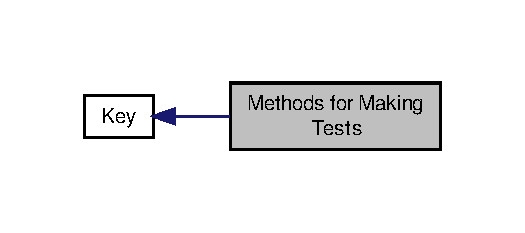
\includegraphics[width=253pt]{group__keytest}
\end{center}
\end{figure}
\subsection*{Functions}
\begin{DoxyCompactItemize}
\item 
int \hyperlink{group__keytest_gaf6e66e12fe04d535a5d1c8218ced803e}{key\+Cmp} (const Key $\ast$k1, const Key $\ast$k2)
\begin{DoxyCompactList}\small\item\em Compare the name of two keys. \end{DoxyCompactList}\item 
int \hyperlink{group__keytest_gaf247df0de7aca04b32ef80e39ef12950}{key\+Need\+Sync} (const Key $\ast$key)
\begin{DoxyCompactList}\small\item\em Test if a key needs to be synced to backend storage. \end{DoxyCompactList}\item 
int \hyperlink{group__keytest_ga03332b5d97c76a4fd2640aca4762b8df}{key\+Is\+Below} (const Key $\ast$key, const Key $\ast$check)
\begin{DoxyCompactList}\small\item\em Check if the key check is below the key key or not. \end{DoxyCompactList}\item 
int \hyperlink{group__keytest_ga0150fb549225d8789e7297b919965e72}{key\+Is\+Directly\+Below} (const Key $\ast$key, const Key $\ast$check)
\begin{DoxyCompactList}\small\item\em Check whether the key {\ttfamily check} is directly below the key {\ttfamily key}. \end{DoxyCompactList}\item 
int \hyperlink{group__keytest_gaa25f699f592031c1a0abc1504d14e13e}{key\+Is\+Inactive} (const Key $\ast$key)
\begin{DoxyCompactList}\small\item\em Check whether a key is inactive. \end{DoxyCompactList}\item 
int \hyperlink{group__keytest_ga9526b371087564e43e3dff8ad0dac949}{key\+Is\+Binary} (const Key $\ast$key)
\begin{DoxyCompactList}\small\item\em Check if a key is binary type. \end{DoxyCompactList}\item 
int \hyperlink{group__keytest_gaea7670778abd07fee0fe8ac12a149190}{key\+Is\+String} (const Key $\ast$key)
\begin{DoxyCompactList}\small\item\em Check if a key is string type. \end{DoxyCompactList}\end{DoxyCompactItemize}


\subsection{Detailed Description}
Methods to do various tests on Keys. 

To use them\+: 
\begin{DoxyCode}
\textcolor{preprocessor}{#include <kdb.h>}
\end{DoxyCode}
 

\subsection{Function Documentation}
\mbox{\Hypertarget{group__keytest_gaf6e66e12fe04d535a5d1c8218ced803e}\label{group__keytest_gaf6e66e12fe04d535a5d1c8218ced803e}} 
\index{Methods for Making Tests@{Methods for Making Tests}!key\+Cmp@{key\+Cmp}}
\index{key\+Cmp@{key\+Cmp}!Methods for Making Tests@{Methods for Making Tests}}
\subsubsection{\texorpdfstring{key\+Cmp()}{keyCmp()}}
{\footnotesize\ttfamily int key\+Cmp (\begin{DoxyParamCaption}\item[{const Key $\ast$}]{k1,  }\item[{const Key $\ast$}]{k2 }\end{DoxyParamCaption})}



Compare the name of two keys. 

\begin{DoxyReturn}{Returns}
a number less than, equal to or greater than zero if k1 is found, respectively, to be less than, to match, or be greater than k2.
\end{DoxyReturn}
The comparison is based on a strcmp of the keynames, and iff they match a strcmp of the owner will be used to distuingish. If even this matches the keys are found to be exactly the same and 0 is returned. These two keys can\textquotesingle{}t be used in the same Key\+Set.

\hyperlink{group__keytest_gaf6e66e12fe04d535a5d1c8218ced803e}{key\+Cmp()} defines the sorting order for a Key\+Set.

The following 3 points are the rules for null values\+:


\begin{DoxyItemize}
\item A null pointer will be found to be smaller than every other key. If both are null pointers, 0 is returned.
\item A null name will be found to be smaller than every other name. If both are null names, 0 is returned.
\end{DoxyItemize}

If the name is equal then\+:


\begin{DoxyItemize}
\item No owner will be found to be smaller then every other owner. If both don\textquotesingle{}t have an owner, 0 is returned.
\end{DoxyItemize}

\begin{DoxyNote}{Note}
the owner will only be used if the names are equal.
\end{DoxyNote}
Given any Keys k1 and k2 constructed with \hyperlink{group__key_gad23c65b44bf48d773759e1f9a4d43b89}{key\+New()}, following equation hold true\+:


\begin{DoxyCodeInclude}
        succeed\_if (\hyperlink{group__keytest_gaf6e66e12fe04d535a5d1c8218ced803e}{keyCmp} (0, 0) == 0, \textcolor{stringliteral}{"all null pointers same"});
        succeed\_if (\hyperlink{group__keytest_gaf6e66e12fe04d535a5d1c8218ced803e}{keyCmp} (k1, 0) == 1, \textcolor{stringliteral}{"null pointer is smaller"});
        succeed\_if (\hyperlink{group__keytest_gaf6e66e12fe04d535a5d1c8218ced803e}{keyCmp} (0, k2) == -1, \textcolor{stringliteral}{"null pointer is smaller"});
\end{DoxyCodeInclude}
 Here are some more examples\+: 
\begin{DoxyCode}
Key *k1 = \hyperlink{group__key_gad23c65b44bf48d773759e1f9a4d43b89}{keyNew}(\textcolor{stringliteral}{"user/a"}, \hyperlink{group__key_gga9b703ca49f48b482def322b77d3e6bc8aa8adb6fcb92dec58fb19410eacfdd403}{KEY\_END});
Key *k2 = \hyperlink{group__key_gad23c65b44bf48d773759e1f9a4d43b89}{keyNew}(\textcolor{stringliteral}{"user/b"}, \hyperlink{group__key_gga9b703ca49f48b482def322b77d3e6bc8aa8adb6fcb92dec58fb19410eacfdd403}{KEY\_END});

\textcolor{comment}{// keyCmp(k1,k2) < 0}
\textcolor{comment}{// keyCmp(k2,k1) > 0}
\end{DoxyCode}


And even more\+: 
\begin{DoxyCode}
Key *k1 = \hyperlink{group__key_gad23c65b44bf48d773759e1f9a4d43b89}{keyNew}(\textcolor{stringliteral}{"user/a"}, \hyperlink{group__key_gga9b703ca49f48b482def322b77d3e6bc8a77ca60362fa8daca8d5347db4385068b}{KEY\_OWNER}, \textcolor{stringliteral}{"markus"}, \hyperlink{group__key_gga9b703ca49f48b482def322b77d3e6bc8aa8adb6fcb92dec58fb19410eacfdd403}{KEY\_END});
Key *k2 = \hyperlink{group__key_gad23c65b44bf48d773759e1f9a4d43b89}{keyNew}(\textcolor{stringliteral}{"user/a"}, \hyperlink{group__key_gga9b703ca49f48b482def322b77d3e6bc8a77ca60362fa8daca8d5347db4385068b}{KEY\_OWNER}, \textcolor{stringliteral}{"max"}, \hyperlink{group__key_gga9b703ca49f48b482def322b77d3e6bc8aa8adb6fcb92dec58fb19410eacfdd403}{KEY\_END});

\textcolor{comment}{// keyCmp(k1,k2) < 0}
\textcolor{comment}{// keyCmp(k2,k1) > 0}
\end{DoxyCode}


Do not strcmp the \hyperlink{group__keyname_ga8e805c726a60da921d3736cda7813513}{key\+Name()} yourself because the result differs from simple ascii comparison.


\begin{DoxyParams}{Parameters}
{\em k1} & the first key object to compare with \\
\hline
{\em k2} & the second key object to compare with\\
\hline
\end{DoxyParams}
\begin{DoxySeeAlso}{See also}
\hyperlink{group__keyset_gaa5a1d467a4d71041edce68ea7748ce45}{ks\+Append\+Key()}, \hyperlink{group__keyset_ga21eb9c3a14a604ee3a8bdc779232e7b7}{ks\+Append()} will compare keys when appending 

\hyperlink{group__keyset_ga60f1ddcf23272f2b29b90e92ebe9b56f}{ks\+Lookup()} will compare keys during searching 
\end{DoxySeeAlso}
\mbox{\Hypertarget{group__keytest_ga03332b5d97c76a4fd2640aca4762b8df}\label{group__keytest_ga03332b5d97c76a4fd2640aca4762b8df}} 
\index{Methods for Making Tests@{Methods for Making Tests}!key\+Is\+Below@{key\+Is\+Below}}
\index{key\+Is\+Below@{key\+Is\+Below}!Methods for Making Tests@{Methods for Making Tests}}
\subsubsection{\texorpdfstring{key\+Is\+Below()}{keyIsBelow()}}
{\footnotesize\ttfamily int key\+Is\+Below (\begin{DoxyParamCaption}\item[{const Key $\ast$}]{key,  }\item[{const Key $\ast$}]{check }\end{DoxyParamCaption})}



Check if the key check is below the key key or not. 

Example\+: \begin{DoxyVerb}key user/sw/app
check user/sw/app/key
\end{DoxyVerb}


returns true because check is below key

Example\+: \begin{DoxyVerb}key user/sw/app
check user/sw/app/folder/key
\end{DoxyVerb}


returns also true because check is indirect below key

Obviously, there is no key above a namespace (e.\+g. user, system, /)\+:

\begin{DoxyVerb}key *
check user
\end{DoxyVerb}



\begin{DoxyParams}{Parameters}
{\em key} & the key object to work with \\
\hline
{\em check} & the key to find the relative position of \\
\hline
\end{DoxyParams}

\begin{DoxyRetVals}{Return values}
{\em 1} & if check is below key \\
\hline
{\em 0} & if it is not below or if it is the same key \\
\hline
{\em -\/1} & if key or check is null \\
\hline
\end{DoxyRetVals}
\begin{DoxySeeAlso}{See also}
\hyperlink{group__keyname_ga7699091610e7f3f43d2949514a4b35d9}{key\+Set\+Name()}, \hyperlink{group__keyname_gab29a850168d9b31c9529e90cf9ab68be}{key\+Get\+Name()}, \hyperlink{group__keytest_ga0150fb549225d8789e7297b919965e72}{key\+Is\+Directly\+Below()} 
\end{DoxySeeAlso}
\mbox{\Hypertarget{group__keytest_ga9526b371087564e43e3dff8ad0dac949}\label{group__keytest_ga9526b371087564e43e3dff8ad0dac949}} 
\index{Methods for Making Tests@{Methods for Making Tests}!key\+Is\+Binary@{key\+Is\+Binary}}
\index{key\+Is\+Binary@{key\+Is\+Binary}!Methods for Making Tests@{Methods for Making Tests}}
\subsubsection{\texorpdfstring{key\+Is\+Binary()}{keyIsBinary()}}
{\footnotesize\ttfamily int key\+Is\+Binary (\begin{DoxyParamCaption}\item[{const Key $\ast$}]{key }\end{DoxyParamCaption})}



Check if a key is binary type. 

The function checks if the key is a binary. Opposed to string values binary values can have \textquotesingle{}\textbackslash{}0\textquotesingle{} inside the value and may not be terminated by a null character. Their disadvantage is that you need to pass their size.

Make sure to use this function and don\textquotesingle{}t test the binary type another way to ensure compatibility and to write less error prone programs.


\begin{DoxyRetVals}{Return values}
{\em 1} & if it is binary \\
\hline
{\em 0} & if it is not \\
\hline
{\em -\/1} & on N\+U\+LL pointer \\
\hline
\end{DoxyRetVals}
\begin{DoxySeeAlso}{See also}
\hyperlink{group__keyvalue_ga4c0d8a4a11174197699c231e0b5c3c84}{key\+Get\+Binary()}, \hyperlink{group__keyvalue_gaa50a5358fd328d373a45f395fa1b99e7}{key\+Set\+Binary()} 
\end{DoxySeeAlso}

\begin{DoxyParams}{Parameters}
{\em key} & the key to check \\
\hline
\end{DoxyParams}
\mbox{\Hypertarget{group__keytest_ga0150fb549225d8789e7297b919965e72}\label{group__keytest_ga0150fb549225d8789e7297b919965e72}} 
\index{Methods for Making Tests@{Methods for Making Tests}!key\+Is\+Directly\+Below@{key\+Is\+Directly\+Below}}
\index{key\+Is\+Directly\+Below@{key\+Is\+Directly\+Below}!Methods for Making Tests@{Methods for Making Tests}}
\subsubsection{\texorpdfstring{key\+Is\+Directly\+Below()}{keyIsDirectlyBelow()}}
{\footnotesize\ttfamily int key\+Is\+Directly\+Below (\begin{DoxyParamCaption}\item[{const Key $\ast$}]{key,  }\item[{const Key $\ast$}]{check }\end{DoxyParamCaption})}



Check whether the key {\ttfamily check} is directly below the key {\ttfamily key}. 

\begin{DoxyVerb}Example:
key user/sw/app
check user/sw/app/key

returns true because check is below key

Example:
key user/sw/app
check user/sw/app/folder/key

does not return true, because there is only an indirect relation
\end{DoxyVerb}



\begin{DoxyParams}{Parameters}
{\em key} & the key object to work with \\
\hline
{\em check} & the key to find the relative position of \\
\hline
\end{DoxyParams}

\begin{DoxyRetVals}{Return values}
{\em 1} & if check is below key \\
\hline
{\em 0} & if it is not below or if it is the same key \\
\hline
{\em -\/1} & on null pointer \\
\hline
\end{DoxyRetVals}
\begin{DoxySeeAlso}{See also}
\hyperlink{group__keytest_ga03332b5d97c76a4fd2640aca4762b8df}{key\+Is\+Below()}, \hyperlink{group__keyname_ga7699091610e7f3f43d2949514a4b35d9}{key\+Set\+Name()}, \hyperlink{group__keyname_gab29a850168d9b31c9529e90cf9ab68be}{key\+Get\+Name()} 
\end{DoxySeeAlso}
\mbox{\Hypertarget{group__keytest_gaa25f699f592031c1a0abc1504d14e13e}\label{group__keytest_gaa25f699f592031c1a0abc1504d14e13e}} 
\index{Methods for Making Tests@{Methods for Making Tests}!key\+Is\+Inactive@{key\+Is\+Inactive}}
\index{key\+Is\+Inactive@{key\+Is\+Inactive}!Methods for Making Tests@{Methods for Making Tests}}
\subsubsection{\texorpdfstring{key\+Is\+Inactive()}{keyIsInactive()}}
{\footnotesize\ttfamily int key\+Is\+Inactive (\begin{DoxyParamCaption}\item[{const Key $\ast$}]{key }\end{DoxyParamCaption})}



Check whether a key is inactive. 

In Elektra terminology a hierarchy of keys is inactive if the rootkey\textquotesingle{}s basename starts with \textquotesingle{}.\textquotesingle{}. So a key is also inactive if it is below an inactive key. For example, user/key/.hidden is inactive and so is user/.hidden/below.

Inactive keys should not have any meaning to applications, they are only a convention reserved for users and administrators. To automatically remove all inactive keys for an application, consider to use the hidden plugin.


\begin{DoxyParams}{Parameters}
{\em key} & the key object to work with \\
\hline
\end{DoxyParams}

\begin{DoxyRetVals}{Return values}
{\em 1} & if the key is inactive \\
\hline
{\em 0} & if the key is active \\
\hline
{\em -\/1} & on N\+U\+LL pointer or when key has no name \\
\hline
\end{DoxyRetVals}
\mbox{\Hypertarget{group__keytest_gaea7670778abd07fee0fe8ac12a149190}\label{group__keytest_gaea7670778abd07fee0fe8ac12a149190}} 
\index{Methods for Making Tests@{Methods for Making Tests}!key\+Is\+String@{key\+Is\+String}}
\index{key\+Is\+String@{key\+Is\+String}!Methods for Making Tests@{Methods for Making Tests}}
\subsubsection{\texorpdfstring{key\+Is\+String()}{keyIsString()}}
{\footnotesize\ttfamily int key\+Is\+String (\begin{DoxyParamCaption}\item[{const Key $\ast$}]{key }\end{DoxyParamCaption})}



Check if a key is string type. 

String values are null terminated and are not allowed to have any \textquotesingle{}\textbackslash{}0\textquotesingle{} characters inside the string.

Make sure to use this function and don\textquotesingle{}t test the string type another way to ensure compatibility and to write less error prone programs.


\begin{DoxyRetVals}{Return values}
{\em 1} & if it is string \\
\hline
{\em 0} & if it is not \\
\hline
{\em -\/1} & on N\+U\+LL pointer \\
\hline
\end{DoxyRetVals}
\begin{DoxySeeAlso}{See also}
\hyperlink{group__keyvalue_ga41b9fac5ccddafe407fc0ae1e2eb8778}{key\+Get\+String()}, \hyperlink{group__keyvalue_ga622bde1eb0e0c4994728331326340ef2}{key\+Set\+String()} 
\end{DoxySeeAlso}

\begin{DoxyParams}{Parameters}
{\em key} & the key to check \\
\hline
\end{DoxyParams}
\mbox{\Hypertarget{group__keytest_gaf247df0de7aca04b32ef80e39ef12950}\label{group__keytest_gaf247df0de7aca04b32ef80e39ef12950}} 
\index{Methods for Making Tests@{Methods for Making Tests}!key\+Need\+Sync@{key\+Need\+Sync}}
\index{key\+Need\+Sync@{key\+Need\+Sync}!Methods for Making Tests@{Methods for Making Tests}}
\subsubsection{\texorpdfstring{key\+Need\+Sync()}{keyNeedSync()}}
{\footnotesize\ttfamily int key\+Need\+Sync (\begin{DoxyParamCaption}\item[{const Key $\ast$}]{key }\end{DoxyParamCaption})}



Test if a key needs to be synced to backend storage. 

If any key modification took place the key will be flagged so that \hyperlink{group__kdb_ga11436b058408f83d303ca5e996832bcf}{kdb\+Set()} knows which keys were modified and which not.

After \hyperlink{group__key_gad23c65b44bf48d773759e1f9a4d43b89}{key\+New()} the flag will normally be set, but after \hyperlink{group__kdb_ga28e385fd9cb7ccfe0b2f1ed2f62453a1}{kdb\+Get()} and \hyperlink{group__kdb_ga11436b058408f83d303ca5e996832bcf}{kdb\+Set()} the flag will be removed. When you modify the key the flag will be set again.

In your application you can make use of that flag to know if you changed something in a key after a \hyperlink{group__kdb_ga28e385fd9cb7ccfe0b2f1ed2f62453a1}{kdb\+Get()} or \hyperlink{group__kdb_ga11436b058408f83d303ca5e996832bcf}{kdb\+Set()}.

\begin{DoxyNote}{Note}
Note that the sync status will be updated on any change, including metadata.
\end{DoxyNote}
\begin{DoxyRefDesc}{Deprecated}
\item[\hyperlink{deprecated__deprecated000012}{Deprecated}]The handling of synchronization is done internally and does not need to be checked by neither application nor plugins.\end{DoxyRefDesc}


\begin{DoxySeeAlso}{See also}
after \hyperlink{group__key_gad23c65b44bf48d773759e1f9a4d43b89}{key\+New()}, \hyperlink{group__key_gae6ec6a60cc4b8c1463fa08623d056ce3}{key\+Dup()} keys need sync
\end{DoxySeeAlso}

\begin{DoxyParams}{Parameters}
{\em key} & the key object to work with \\
\hline
\end{DoxyParams}

\begin{DoxyRetVals}{Return values}
{\em 1} & if {\ttfamily key} was changed in memory, 0 otherwise \\
\hline
{\em -\/1} & on N\+U\+LL pointer \\
\hline
\end{DoxyRetVals}

\hypertarget{group__keyvalue}{}\section{Value Manipulation Methods}
\label{group__keyvalue}\index{Value Manipulation Methods@{Value Manipulation Methods}}


Methods to do various operations on Key values.  


Collaboration diagram for Value Manipulation Methods\+:
\nopagebreak
\begin{figure}[H]
\begin{center}
\leavevmode
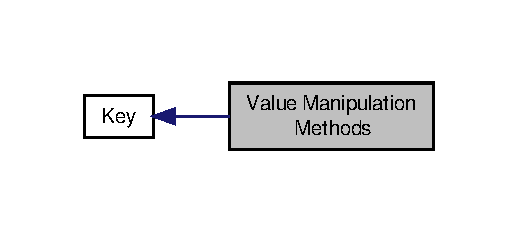
\includegraphics[width=249pt]{group__keyvalue}
\end{center}
\end{figure}
\subsection*{Functions}
\begin{DoxyCompactItemize}
\item 
const void $\ast$ \hyperlink{group__keyvalue_ga6f29609c5da53c6dc26a98678d5752af}{key\+Value} (const Key $\ast$key)
\begin{DoxyCompactList}\small\item\em Return a pointer to the real internal {\ttfamily key} value. \end{DoxyCompactList}\item 
const char $\ast$ \hyperlink{group__keyvalue_ga880936f2481d28e6e2acbe7486a21d05}{key\+String} (const Key $\ast$key)
\begin{DoxyCompactList}\small\item\em Get the c-\/string representing the value. \end{DoxyCompactList}\item 
ssize\+\_\+t \hyperlink{group__keyvalue_gae326672fffb7474abfe9baf53b73217e}{key\+Get\+Value\+Size} (const Key $\ast$key)
\begin{DoxyCompactList}\small\item\em Returns the number of bytes needed to store the key value, including the N\+U\+LL terminator. \end{DoxyCompactList}\item 
ssize\+\_\+t \hyperlink{group__keyvalue_ga41b9fac5ccddafe407fc0ae1e2eb8778}{key\+Get\+String} (const Key $\ast$key, char $\ast$returned\+String, size\+\_\+t max\+Size)
\begin{DoxyCompactList}\small\item\em Get the value of a key as a string. \end{DoxyCompactList}\item 
ssize\+\_\+t \hyperlink{group__keyvalue_ga622bde1eb0e0c4994728331326340ef2}{key\+Set\+String} (Key $\ast$key, const char $\ast$new\+String\+Value)
\begin{DoxyCompactList}\small\item\em Set the value for {\ttfamily key} as {\ttfamily new\+String\+Value}. \end{DoxyCompactList}\item 
ssize\+\_\+t \hyperlink{group__keyvalue_ga4c0d8a4a11174197699c231e0b5c3c84}{key\+Get\+Binary} (const Key $\ast$key, void $\ast$returned\+Binary, size\+\_\+t max\+Size)
\begin{DoxyCompactList}\small\item\em Get the value of a key as a binary. \end{DoxyCompactList}\item 
ssize\+\_\+t \hyperlink{group__keyvalue_gaa50a5358fd328d373a45f395fa1b99e7}{key\+Set\+Binary} (Key $\ast$key, const void $\ast$new\+Binary, size\+\_\+t data\+Size)
\begin{DoxyCompactList}\small\item\em Set the value of a key as a binary. \end{DoxyCompactList}\end{DoxyCompactItemize}


\subsection{Detailed Description}
Methods to do various operations on Key values. 

A key can contain a value in different format. The most likely situation is, that the value is interpreted as text. Use \hyperlink{group__keyvalue_ga41b9fac5ccddafe407fc0ae1e2eb8778}{key\+Get\+String()} for that. You can save any Unicode Symbols and Elektra will take care that you get the same back, independent of your current environment.

In some situations this idea fails. When you need exactly the same value back without any interpretation of the characters, there is \hyperlink{group__keyvalue_gaa50a5358fd328d373a45f395fa1b99e7}{key\+Set\+Binary()}. If you use that, its very likely that your Configuration is not according to the standard. Also for Numbers, Booleans and Date you should use \hyperlink{group__keyvalue_ga41b9fac5ccddafe407fc0ae1e2eb8778}{key\+Get\+String()}. To do so, you might use strtod() strtol() and then atol() or atof() to convert back.

To use them\+: 
\begin{DoxyCode}
\textcolor{preprocessor}{#include <kdb.h>}
\end{DoxyCode}
 

\subsection{Function Documentation}
\mbox{\Hypertarget{group__keyvalue_ga4c0d8a4a11174197699c231e0b5c3c84}\label{group__keyvalue_ga4c0d8a4a11174197699c231e0b5c3c84}} 
\index{Value Manipulation Methods@{Value Manipulation Methods}!key\+Get\+Binary@{key\+Get\+Binary}}
\index{key\+Get\+Binary@{key\+Get\+Binary}!Value Manipulation Methods@{Value Manipulation Methods}}
\subsubsection{\texorpdfstring{key\+Get\+Binary()}{keyGetBinary()}}
{\footnotesize\ttfamily ssize\+\_\+t key\+Get\+Binary (\begin{DoxyParamCaption}\item[{const Key $\ast$}]{key,  }\item[{void $\ast$}]{returned\+Binary,  }\item[{size\+\_\+t}]{max\+Size }\end{DoxyParamCaption})}



Get the value of a key as a binary. 

If the type is not binary -\/1 will be returned.

When the binary data is empty (this is not the same as \char`\"{}\char`\"{}!) 0 will be returned and the returned\+Binary will not be changed.

For string values see \hyperlink{group__keyvalue_ga41b9fac5ccddafe407fc0ae1e2eb8778}{key\+Get\+String()} and \hyperlink{group__keytest_gaea7670778abd07fee0fe8ac12a149190}{key\+Is\+String()}.

When the returned\+Binary is to small to hold the data (its maximum size is given by max\+Size), the returned\+Binary will not be changed and -\/1 is returned.

\begin{DoxyParagraph}{Example\+:}

\begin{DoxyCode}
Key *key = \hyperlink{group__key_gad23c65b44bf48d773759e1f9a4d43b89}{keyNew} (\textcolor{stringliteral}{"user/keyname"}, KEY\_TYPE, KEY\_TYPE\_BINARY, \hyperlink{group__key_gga91fb3178848bd682000958089abbaf40aa8adb6fcb92dec58fb19410eacfdd403}{KEY\_END});
\textcolor{keywordtype}{char} buffer[300];

\textcolor{keywordflow}{if} (\hyperlink{group__keyvalue_ga4c0d8a4a11174197699c231e0b5c3c84}{keyGetBinary}(key,buffer,\textcolor{keyword}{sizeof}(buffer)) == -1)
\{
        \textcolor{comment}{// handle error}
\}
\end{DoxyCode}

\end{DoxyParagraph}

\begin{DoxyParams}{Parameters}
{\em key} & the object to gather the value from \\
\hline
{\em returned\+Binary} & pre-\/allocated memory to store a copy of the key value \\
\hline
{\em max\+Size} & number of bytes of pre-\/allocated memory in {\ttfamily returned\+Binary} \\
\hline
\end{DoxyParams}
\begin{DoxyReturn}{Returns}
the number of bytes actually copied to {\ttfamily returned\+Binary} 
\end{DoxyReturn}

\begin{DoxyRetVals}{Return values}
{\em 0} & if the binary is empty \\
\hline
{\em -\/1} & on N\+U\+LL pointers \\
\hline
{\em -\/1} & if max\+Size is 0 \\
\hline
{\em -\/1} & if max\+Size is too small for string \\
\hline
{\em -\/1} & if max\+Size is larger than S\+S\+I\+Z\+E\+\_\+\+M\+AX \\
\hline
{\em -\/1} & on type mismatch\+: binary expected, but found string \\
\hline
\end{DoxyRetVals}
\begin{DoxySeeAlso}{See also}
\hyperlink{group__keyvalue_ga6f29609c5da53c6dc26a98678d5752af}{key\+Value()}, \hyperlink{group__keyvalue_gae326672fffb7474abfe9baf53b73217e}{key\+Get\+Value\+Size()}, \hyperlink{group__keyvalue_gaa50a5358fd328d373a45f395fa1b99e7}{key\+Set\+Binary()} 

\hyperlink{group__keyvalue_ga41b9fac5ccddafe407fc0ae1e2eb8778}{key\+Get\+String()} and \hyperlink{group__keyvalue_ga622bde1eb0e0c4994728331326340ef2}{key\+Set\+String()} as preferred alternative to binary 

\hyperlink{group__keytest_ga9526b371087564e43e3dff8ad0dac949}{key\+Is\+Binary()} to see how to check for binary type 
\end{DoxySeeAlso}
\mbox{\Hypertarget{group__keyvalue_ga41b9fac5ccddafe407fc0ae1e2eb8778}\label{group__keyvalue_ga41b9fac5ccddafe407fc0ae1e2eb8778}} 
\index{Value Manipulation Methods@{Value Manipulation Methods}!key\+Get\+String@{key\+Get\+String}}
\index{key\+Get\+String@{key\+Get\+String}!Value Manipulation Methods@{Value Manipulation Methods}}
\subsubsection{\texorpdfstring{key\+Get\+String()}{keyGetString()}}
{\footnotesize\ttfamily ssize\+\_\+t key\+Get\+String (\begin{DoxyParamCaption}\item[{const Key $\ast$}]{key,  }\item[{char $\ast$}]{returned\+String,  }\item[{size\+\_\+t}]{max\+Size }\end{DoxyParamCaption})}



Get the value of a key as a string. 

When there is no value inside the string, 1 will be returned and the returned\+String will be empty \char`\"{}\char`\"{} to avoid programming errors that old strings are shown to the user.

For binary values see \hyperlink{group__keyvalue_ga4c0d8a4a11174197699c231e0b5c3c84}{key\+Get\+Binary()} and \hyperlink{group__keytest_ga9526b371087564e43e3dff8ad0dac949}{key\+Is\+Binary()}.

\begin{DoxyParagraph}{Example\+:}

\begin{DoxyCode}
Key *key = \hyperlink{group__key_gad23c65b44bf48d773759e1f9a4d43b89}{keyNew} (\textcolor{stringliteral}{"user/keyname"}, \hyperlink{group__key_gga91fb3178848bd682000958089abbaf40aa8adb6fcb92dec58fb19410eacfdd403}{KEY\_END});
\textcolor{keywordtype}{char} buffer[300];

\textcolor{keywordflow}{if} (\hyperlink{group__keyvalue_ga41b9fac5ccddafe407fc0ae1e2eb8778}{keyGetString}(key,buffer,\textcolor{keyword}{sizeof}(buffer)) == -1)
\{
        \textcolor{comment}{// handle error}
\} \textcolor{keywordflow}{else} \{
        printf (\textcolor{stringliteral}{"buffer: %s\(\backslash\)n"}, buffer);
\}
\end{DoxyCode}

\end{DoxyParagraph}

\begin{DoxyParams}{Parameters}
{\em key} & the object to gather the value from \\
\hline
{\em returned\+String} & pre-\/allocated memory to store a copy of the key value \\
\hline
{\em max\+Size} & number of bytes of allocated memory in {\ttfamily returned\+String} \\
\hline
\end{DoxyParams}
\begin{DoxyReturn}{Returns}
the number of bytes actually copied to {\ttfamily returned\+String}, including final N\+U\+LL 
\end{DoxyReturn}

\begin{DoxyRetVals}{Return values}
{\em 1} & if the string is empty \\
\hline
{\em -\/1} & on any N\+U\+LL pointers \\
\hline
{\em -\/1} & on type mismatch\+: string expected, but found binary \\
\hline
{\em -\/1} & max\+Size is 0 \\
\hline
{\em -\/1} & if max\+Size is too small for string \\
\hline
{\em -\/1} & if max\+Size is larger than S\+S\+I\+Z\+E\+\_\+\+M\+AX \\
\hline
\end{DoxyRetVals}
\begin{DoxySeeAlso}{See also}
\hyperlink{group__keyvalue_ga6f29609c5da53c6dc26a98678d5752af}{key\+Value()}, \hyperlink{group__keyvalue_gae326672fffb7474abfe9baf53b73217e}{key\+Get\+Value\+Size()}, \hyperlink{group__keyvalue_ga622bde1eb0e0c4994728331326340ef2}{key\+Set\+String()}, \hyperlink{group__keyvalue_ga880936f2481d28e6e2acbe7486a21d05}{key\+String()} 

\hyperlink{group__keyvalue_ga4c0d8a4a11174197699c231e0b5c3c84}{key\+Get\+Binary()} for working with binary data 
\end{DoxySeeAlso}
\mbox{\Hypertarget{group__keyvalue_gae326672fffb7474abfe9baf53b73217e}\label{group__keyvalue_gae326672fffb7474abfe9baf53b73217e}} 
\index{Value Manipulation Methods@{Value Manipulation Methods}!key\+Get\+Value\+Size@{key\+Get\+Value\+Size}}
\index{key\+Get\+Value\+Size@{key\+Get\+Value\+Size}!Value Manipulation Methods@{Value Manipulation Methods}}
\subsubsection{\texorpdfstring{key\+Get\+Value\+Size()}{keyGetValueSize()}}
{\footnotesize\ttfamily ssize\+\_\+t key\+Get\+Value\+Size (\begin{DoxyParamCaption}\item[{const Key $\ast$}]{key }\end{DoxyParamCaption})}



Returns the number of bytes needed to store the key value, including the N\+U\+LL terminator. 

It returns the correct size, independent of the Key Type. If it is a binary there might be \textquotesingle{}\textbackslash{}0\textquotesingle{} values in it.

For an empty string you need one byte to store the ending N\+U\+LL. For that reason 1 is returned. This is not true for binary data, so there might be returned 0 too.

A binary key has no \textquotesingle{}\textbackslash{}0\textquotesingle{} termination. String types have it, so to there length will be added 1 to have enough space to store it.

This method can be used with \hyperlink{internal_8c_a35cdc2e5caed3454cb73b4fc7f37858c}{elektra\+Malloc()} before \hyperlink{group__keyvalue_ga41b9fac5ccddafe407fc0ae1e2eb8778}{key\+Get\+String()} or \hyperlink{group__keyvalue_ga4c0d8a4a11174197699c231e0b5c3c84}{key\+Get\+Binary()} is called.


\begin{DoxyCode}
\textcolor{keywordtype}{char} *buffer;
buffer = \hyperlink{internal_8c_a35cdc2e5caed3454cb73b4fc7f37858c}{elektraMalloc} (\hyperlink{group__keyvalue_gae326672fffb7474abfe9baf53b73217e}{keyGetValueSize} (key));
\textcolor{comment}{// use this buffer to store the value (binary or string)}
\textcolor{comment}{// pass keyGetValueSize (key) for maxSize}
\end{DoxyCode}



\begin{DoxyParams}{Parameters}
{\em key} & the key object to work with \\
\hline
\end{DoxyParams}
\begin{DoxyReturn}{Returns}
the number of bytes needed to store the key value 
\end{DoxyReturn}

\begin{DoxyRetVals}{Return values}
{\em 1} & when there is no data and type is not binary \\
\hline
{\em 0} & when there is no data and type is binary \\
\hline
{\em -\/1} & on null pointer \\
\hline
\end{DoxyRetVals}
\begin{DoxySeeAlso}{See also}
\hyperlink{group__keyvalue_ga41b9fac5ccddafe407fc0ae1e2eb8778}{key\+Get\+String()}, \hyperlink{group__keyvalue_ga4c0d8a4a11174197699c231e0b5c3c84}{key\+Get\+Binary()}, \hyperlink{group__keyvalue_ga6f29609c5da53c6dc26a98678d5752af}{key\+Value()} 
\end{DoxySeeAlso}
\mbox{\Hypertarget{group__keyvalue_gaa50a5358fd328d373a45f395fa1b99e7}\label{group__keyvalue_gaa50a5358fd328d373a45f395fa1b99e7}} 
\index{Value Manipulation Methods@{Value Manipulation Methods}!key\+Set\+Binary@{key\+Set\+Binary}}
\index{key\+Set\+Binary@{key\+Set\+Binary}!Value Manipulation Methods@{Value Manipulation Methods}}
\subsubsection{\texorpdfstring{key\+Set\+Binary()}{keySetBinary()}}
{\footnotesize\ttfamily ssize\+\_\+t key\+Set\+Binary (\begin{DoxyParamCaption}\item[{Key $\ast$}]{key,  }\item[{const void $\ast$}]{new\+Binary,  }\item[{size\+\_\+t}]{data\+Size }\end{DoxyParamCaption})}



Set the value of a key as a binary. 

A private copy of {\ttfamily new\+Binary} will allocated and saved inside {\ttfamily key}, so the parameter can be deallocated after the call.

Binary values might be encoded in another way then string values depending on the plugin. Typically character encodings should not take place on binary data. Consider using a string key instead.

When new\+Binary is a N\+U\+LL pointer the binary will be freed and 0 will be returned.

\begin{DoxyNote}{Note}
The metadata \char`\"{}binary\char`\"{} will be set to mark that the key is binary from now on. When the key is already binary the metadata won\textquotesingle{}t be changed. This will only happen in the successful case, but not when -\/1 is returned.
\end{DoxyNote}

\begin{DoxyParams}{Parameters}
{\em key} & the object on which to set the value \\
\hline
{\em new\+Binary} & is a pointer to any binary data or N\+U\+LL to free the previous set data \\
\hline
{\em data\+Size} & number of bytes to copy from {\ttfamily new\+Binary} \\
\hline
\end{DoxyParams}
\begin{DoxyReturn}{Returns}
the number of bytes actually copied to internal struct storage 
\end{DoxyReturn}

\begin{DoxyRetVals}{Return values}
{\em 0} & when the internal binary was freed and is now a null pointer \\
\hline
{\em -\/1} & if key is a N\+U\+LL pointer \\
\hline
{\em -\/1} & when data\+Size is 0 (but new\+Binary not N\+U\+LL) or larger than S\+S\+I\+Z\+E\+\_\+\+M\+AX \\
\hline
\end{DoxyRetVals}
\begin{DoxySeeAlso}{See also}
\hyperlink{group__keyvalue_ga4c0d8a4a11174197699c231e0b5c3c84}{key\+Get\+Binary()} 

\hyperlink{group__keytest_ga9526b371087564e43e3dff8ad0dac949}{key\+Is\+Binary()} to check if the type is binary 

\hyperlink{group__keyvalue_ga41b9fac5ccddafe407fc0ae1e2eb8778}{key\+Get\+String()} and \hyperlink{group__keyvalue_ga622bde1eb0e0c4994728331326340ef2}{key\+Set\+String()} as preferred alternative to binary 
\end{DoxySeeAlso}
\mbox{\Hypertarget{group__keyvalue_ga622bde1eb0e0c4994728331326340ef2}\label{group__keyvalue_ga622bde1eb0e0c4994728331326340ef2}} 
\index{Value Manipulation Methods@{Value Manipulation Methods}!key\+Set\+String@{key\+Set\+String}}
\index{key\+Set\+String@{key\+Set\+String}!Value Manipulation Methods@{Value Manipulation Methods}}
\subsubsection{\texorpdfstring{key\+Set\+String()}{keySetString()}}
{\footnotesize\ttfamily ssize\+\_\+t key\+Set\+String (\begin{DoxyParamCaption}\item[{Key $\ast$}]{key,  }\item[{const char $\ast$}]{new\+String\+Value }\end{DoxyParamCaption})}



Set the value for {\ttfamily key} as {\ttfamily new\+String\+Value}. 

The function will allocate and save a private copy of {\ttfamily new\+String\+Value}, so the parameter can be freed after the call.

String values will be saved in backend storage, when kdb\+Set\+Key() will be called, in U\+T\+F-\/8 universal encoding, regardless of the program\textquotesingle{}s current encoding, when iconv plugin is present.

\begin{DoxyNote}{Note}
The type will be set to K\+E\+Y\+\_\+\+T\+Y\+P\+E\+\_\+\+S\+T\+R\+I\+NG. When the type of the key is already a string type it won\textquotesingle{}t be changed.
\end{DoxyNote}

\begin{DoxyParams}{Parameters}
{\em key} & the key to set the string value \\
\hline
{\em new\+String\+Value} & N\+U\+L\+L-\/terminated text string to be set as {\ttfamily key\textquotesingle{}s} value \\
\hline
\end{DoxyParams}
\begin{DoxyReturn}{Returns}
the number of bytes actually saved in private struct including final N\+U\+LL 
\end{DoxyReturn}

\begin{DoxyRetVals}{Return values}
{\em 1} & if new\+String\+Value is a N\+U\+LL pointer, this will make the string empty (string only containing null termination) \\
\hline
{\em -\/1} & if key is a N\+U\+LL pointer \\
\hline
\end{DoxyRetVals}
\begin{DoxySeeAlso}{See also}
\hyperlink{group__keyvalue_ga41b9fac5ccddafe407fc0ae1e2eb8778}{key\+Get\+String()}, \hyperlink{group__keyvalue_ga6f29609c5da53c6dc26a98678d5752af}{key\+Value()}, \hyperlink{group__keyvalue_ga880936f2481d28e6e2acbe7486a21d05}{key\+String()} 
\end{DoxySeeAlso}
\mbox{\Hypertarget{group__keyvalue_ga880936f2481d28e6e2acbe7486a21d05}\label{group__keyvalue_ga880936f2481d28e6e2acbe7486a21d05}} 
\index{Value Manipulation Methods@{Value Manipulation Methods}!key\+String@{key\+String}}
\index{key\+String@{key\+String}!Value Manipulation Methods@{Value Manipulation Methods}}
\subsubsection{\texorpdfstring{key\+String()}{keyString()}}
{\footnotesize\ttfamily const char$\ast$ key\+String (\begin{DoxyParamCaption}\item[{const Key $\ast$}]{key }\end{DoxyParamCaption})}



Get the c-\/string representing the value. 

Will return (null) on null pointers. Will return (binary) on binary data not ended with a null byte.

It is not checked if it is actually a string, only if it terminates for security reasons.

\begin{DoxyReturn}{Returns}
the c-\/string of the value 
\end{DoxyReturn}

\begin{DoxyRetVals}{Return values}
{\em (null)} & on null keys \\
\hline
{\em \char`\"{}\char`\"{}} & if no data found \\
\hline
{\em (binary)} & on binary keys\\
\hline
\end{DoxyRetVals}

\begin{DoxyParams}{Parameters}
{\em key} & the key object to get the string from \\
\hline
\end{DoxyParams}
\mbox{\Hypertarget{group__keyvalue_ga6f29609c5da53c6dc26a98678d5752af}\label{group__keyvalue_ga6f29609c5da53c6dc26a98678d5752af}} 
\index{Value Manipulation Methods@{Value Manipulation Methods}!key\+Value@{key\+Value}}
\index{key\+Value@{key\+Value}!Value Manipulation Methods@{Value Manipulation Methods}}
\subsubsection{\texorpdfstring{key\+Value()}{keyValue()}}
{\footnotesize\ttfamily const void$\ast$ key\+Value (\begin{DoxyParamCaption}\item[{const Key $\ast$}]{key }\end{DoxyParamCaption})}



Return a pointer to the real internal {\ttfamily key} value. 

This is a much more efficient version of \hyperlink{group__keyvalue_ga41b9fac5ccddafe407fc0ae1e2eb8778}{key\+Get\+String()} \hyperlink{group__keyvalue_ga4c0d8a4a11174197699c231e0b5c3c84}{key\+Get\+Binary()}, and you should use it if you are responsible enough to not mess up things. You are not allowed to modify anything in the returned string. If you need a copy of the Value, consider to use \hyperlink{group__keyvalue_ga41b9fac5ccddafe407fc0ae1e2eb8778}{key\+Get\+String()} or \hyperlink{group__keyvalue_ga4c0d8a4a11174197699c231e0b5c3c84}{key\+Get\+Binary()} instead.\hypertarget{group__keyvalue_string}{}\subsection{String Handling}\label{group__keyvalue_string}
If {\ttfamily key} is string (\hyperlink{group__keytest_gaea7670778abd07fee0fe8ac12a149190}{key\+Is\+String()}), you may cast the returned as a {\ttfamily \char`\"{}char $\ast$\char`\"{}} because you\textquotesingle{}ll get a N\+U\+LL terminated regular string.

\hyperlink{group__keyvalue_ga6f29609c5da53c6dc26a98678d5752af}{key\+Value()} returns \char`\"{}\char`\"{} in string mode when there is no value. The reason is 
\begin{DoxyCode}
key=\hyperlink{group__key_gad23c65b44bf48d773759e1f9a4d43b89}{keyNew}(0);
\hyperlink{group__keyvalue_ga622bde1eb0e0c4994728331326340ef2}{keySetString}(key,\textcolor{stringliteral}{""});
\hyperlink{group__keyvalue_ga6f29609c5da53c6dc26a98678d5752af}{keyValue}(key); \textcolor{comment}{// you would expect "" here}
\hyperlink{group__key_ga3df95bbc2494e3e6703ece5639be5bb1}{keyDel}(key);
\end{DoxyCode}
\hypertarget{group__keyvalue_binary}{}\subsection{Binary Data Handling}\label{group__keyvalue_binary}
If the data is binary, the size of the value must be determined by \hyperlink{group__keyvalue_gae326672fffb7474abfe9baf53b73217e}{key\+Get\+Value\+Size()}, any strlen() operations are not suitable to determine the size.

\hyperlink{group__keyvalue_ga6f29609c5da53c6dc26a98678d5752af}{key\+Value()} returns 0 in binary mode when there is no value. The reason is 
\begin{DoxyCode}
key=\hyperlink{group__key_gad23c65b44bf48d773759e1f9a4d43b89}{keyNew}(0);
\hyperlink{group__keyvalue_gaa50a5358fd328d373a45f395fa1b99e7}{keySetBinary}(key, 0, 0);
\hyperlink{group__keyvalue_ga6f29609c5da53c6dc26a98678d5752af}{keyValue}(key); \textcolor{comment}{// you would expect 0 here}

\hyperlink{group__keyvalue_gaa50a5358fd328d373a45f395fa1b99e7}{keySetBinary}(key,\textcolor{stringliteral}{""}, 1);
\hyperlink{group__keyvalue_ga6f29609c5da53c6dc26a98678d5752af}{keyValue}(key); \textcolor{comment}{// you would expect "" (a pointer to '\(\backslash\)0') here}

\textcolor{keywordtype}{int} i=23;
\hyperlink{group__keyvalue_gaa50a5358fd328d373a45f395fa1b99e7}{keySetBinary}(key, (\textcolor{keywordtype}{void}*)&i, 4);
(\textcolor{keywordtype}{int}*)\hyperlink{group__keyvalue_ga6f29609c5da53c6dc26a98678d5752af}{keyValue}(key); \textcolor{comment}{// you would expect a pointer to (int)23 here}
\hyperlink{group__key_ga3df95bbc2494e3e6703ece5639be5bb1}{keyDel}(key);
\end{DoxyCode}


\begin{DoxyNote}{Note}
Note that the Key structure keeps its own size field that is calculated by library internal calls, so to avoid inconsistencies, you must never use the pointer returned by \hyperlink{group__keyvalue_ga6f29609c5da53c6dc26a98678d5752af}{key\+Value()} method to set a new value. Use \hyperlink{group__keyvalue_ga622bde1eb0e0c4994728331326340ef2}{key\+Set\+String()} or \hyperlink{group__keyvalue_gaa50a5358fd328d373a45f395fa1b99e7}{key\+Set\+Binary()} instead.
\end{DoxyNote}
\begin{DoxyWarning}{Warning}
Binary keys will return a N\+U\+LL pointer when there is no data in contrast to \hyperlink{group__keyname_ga8e805c726a60da921d3736cda7813513}{key\+Name()}, \hyperlink{group__keyname_gaaff35e7ca8af5560c47e662ceb9465f5}{key\+Base\+Name()}, \hyperlink{owner_8c_af6485fb8599714b6bbd830cf915ffea5}{key\+Owner()} and \hyperlink{group__meta_gac89fd319783b3457db45b4c09e55274a}{key\+Comment()}. For string value the behaviour is the same.
\end{DoxyWarning}
\begin{DoxyParagraph}{Example\+:}

\begin{DoxyCode}
KDB *handle = \hyperlink{group__kdb_ga6808defe5870f328dd17910aacbdc6ca}{kdbOpen}();
KeySet *ks=\hyperlink{group__keyset_ga671e1aaee3ae9dc13b4834a4ddbd2c3c}{ksNew}(0, \hyperlink{kdbenum_8c_a7a28fce3773b2c873c94ac80b8b4cd54}{KS\_END});
Key *current=0;

kdbGetByName(handle,ks,\textcolor{stringliteral}{"system/sw/my"},\hyperlink{group__keyset_gga98a3d6a4016c9dad9cbd1a99a9c2a45aad9d03b36ee88ca5a774cc01b190c99b8}{KDB\_O\_SORT}|KDB\_O\_RECURSIVE);

\hyperlink{group__keyset_gabe793ff51f1728e3429c84a8a9086b70}{ksRewind}(ks);
\textcolor{keywordflow}{while} (current=\hyperlink{group__keyset_ga317321c9065b5a4b3e33fe1c399bcec9}{ksNext}(ks)) \{
        \textcolor{keywordtype}{size\_t} size=0;

        \textcolor{keywordflow}{if} (keyIsBin(current)) \{
                size=\hyperlink{group__keyvalue_gae326672fffb7474abfe9baf53b73217e}{keyGetValueSize}(current);
                printf(\textcolor{stringliteral}{"Key %s has a value of size %d bytes. Value: <BINARY>\(\backslash\)nComment: %s"},
                        \hyperlink{group__keyname_ga8e805c726a60da921d3736cda7813513}{keyName}(current),
                        size,
                        \hyperlink{group__meta_gac89fd319783b3457db45b4c09e55274a}{keyComment}(current));
        \} \textcolor{keywordflow}{else} \{
                size=\hyperlink{internal_8c_afd676487565d083a6ad5a1381095acd8}{elektraStrLen}((\textcolor{keywordtype}{char} *)\hyperlink{group__keyvalue_ga6f29609c5da53c6dc26a98678d5752af}{keyValue}(current));
                printf(\textcolor{stringliteral}{"Key %s has a value of size %d bytes. Value: %s\(\backslash\)nComment: %s"},
                        \hyperlink{group__keyname_ga8e805c726a60da921d3736cda7813513}{keyName}(current),
                        size,
                        (\textcolor{keywordtype}{char} *)\hyperlink{group__keyvalue_ga6f29609c5da53c6dc26a98678d5752af}{keyValue}(current),
                        \hyperlink{group__meta_gac89fd319783b3457db45b4c09e55274a}{keyComment}(current));
        \}
\}

\hyperlink{group__keyset_ga27e5c16473b02a422238c8d970db7ac8}{ksDel} (ks);
\hyperlink{group__kdb_gadb54dc9fda17ee07deb9444df745c96f}{kdbClose} (handle);
\end{DoxyCode}

\end{DoxyParagraph}

\begin{DoxyParams}{Parameters}
{\em key} & the key object to work with \\
\hline
\end{DoxyParams}
\begin{DoxyReturn}{Returns}
a pointer to internal value 
\end{DoxyReturn}

\begin{DoxyRetVals}{Return values}
{\em \char`\"{}\char`\"{}} & when there is no data and key is not binary \\
\hline
{\em 0} & where there is no data and key is binary \\
\hline
{\em 0} & on N\+U\+LL pointer \\
\hline
\end{DoxyRetVals}
\begin{DoxySeeAlso}{See also}
\hyperlink{group__keyvalue_gae326672fffb7474abfe9baf53b73217e}{key\+Get\+Value\+Size()}, \hyperlink{group__keyvalue_ga41b9fac5ccddafe407fc0ae1e2eb8778}{key\+Get\+String()}, \hyperlink{group__keyvalue_ga4c0d8a4a11174197699c231e0b5c3c84}{key\+Get\+Binary()} 
\end{DoxySeeAlso}

\hypertarget{group__plugin}{\section{Plugins}
\label{group__plugin}\index{Plugins@{Plugins}}
}


Elektra plugin framework.  


\subsection*{Macros}
\begin{DoxyCompactItemize}
\item 
\#define \hyperlink{group__plugin_ga34d1a66f0a6e89cfd20f4014a9975a2a}{E\-L\-E\-K\-T\-R\-A\-\_\-\-P\-L\-U\-G\-I\-N\-\_\-\-F\-U\-N\-C\-T\-I\-O\-N}(module, function)~libelektra\-\_\-\#\#module\#\#\-\_\-\-L\-T\-X\-\_\-elektra\-Plugin\#\#function
\begin{DoxyCompactList}\small\item\em Declare a plugin's function name suitable for compilation variants (see doc/tutorials). \end{DoxyCompactList}\item 
\#define \hyperlink{group__plugin_ga78d616f68bf9fb0942f66478597467c6}{E\-L\-E\-K\-T\-R\-A\-\_\-\-R\-E\-A\-D\-M\-E}(module)~E\-L\-E\-K\-T\-R\-A\-\_\-\-R\-E\-A\-D\-M\-E2(module)
\begin{DoxyCompactList}\small\item\em The filename for inclusion of the readme for compilation variants (see doc/tutorials). \end{DoxyCompactList}\item 
\#define \hyperlink{group__plugin_gaab1842b82272e6d4235b6a71587a64d9}{E\-L\-E\-K\-T\-R\-A\-\_\-\-S\-E\-T\-\_\-\-E\-R\-R\-O\-R}(number, key, text)
\begin{DoxyCompactList}\small\item\em Sets the error in the keys metadata. \end{DoxyCompactList}\item 
\#define \hyperlink{group__plugin_ga3e4fc2c20d8e64bed7a54bb1af882e34}{E\-L\-E\-K\-T\-R\-A\-\_\-\-S\-E\-T\-\_\-\-E\-R\-R\-O\-R\-F}(number, key, formatstring,...)
\begin{DoxyCompactList}\small\item\em Sets the error in the keys metadata. \end{DoxyCompactList}\item 
\#define \hyperlink{group__plugin_ga2bbb3bc3a3bdaf5b34b52de81886a098}{E\-L\-E\-K\-T\-R\-A\-\_\-\-A\-D\-D\-\_\-\-W\-A\-R\-N\-I\-N\-G\-F}(number, key, formatstring,...)
\begin{DoxyCompactList}\small\item\em Adds an warning in the keys metadata. \end{DoxyCompactList}\item 
\#define \hyperlink{group__plugin_ga3da3bdb0f41710adda9eee3d7adac9ff}{E\-L\-E\-K\-T\-R\-A\-\_\-\-A\-D\-D\-\_\-\-W\-A\-R\-N\-I\-N\-G}(number, key, text)
\begin{DoxyCompactList}\small\item\em Adds an warning in the keys metadata. \end{DoxyCompactList}\end{DoxyCompactItemize}
\subsection*{Functions}
\begin{DoxyCompactItemize}
\item 
Plugin $\ast$ \hyperlink{group__plugin_ga8dd092048e972a3f0c9c9f54eb41576e}{elektra\-Plugin\-Export} (const char $\ast$plugin\-Name,...)
\begin{DoxyCompactList}\small\item\em Allows to Export Methods for a Plugin. \end{DoxyCompactList}\item 
Key\-Set $\ast$ \hyperlink{group__plugin_ga644bead796506c172817724051c977c9}{elektra\-Plugin\-Get\-Config} (Plugin $\ast$handle)
\begin{DoxyCompactList}\small\item\em Returns the configuration of that plugin. \end{DoxyCompactList}\item 
void \hyperlink{group__plugin_gaf4b941a52ff55d0ca2a9158d90208ef2}{elektra\-Plugin\-Set\-Data} (Plugin $\ast$plugin, void $\ast$data)
\begin{DoxyCompactList}\small\item\em Store a pointer to any plugin related data. \end{DoxyCompactList}\item 
void $\ast$ \hyperlink{group__plugin_gaafcf3216b46292f222b8cc7828b4dd20}{elektra\-Plugin\-Get\-Data} (Plugin $\ast$plugin)
\begin{DoxyCompactList}\small\item\em Get a pointer to any plugin related data stored before. \end{DoxyCompactList}\item 
int \hyperlink{group__plugin_ga23c2eb3584e38a4d494eb8f91e5e3d8d}{elektra\-Doc\-Open} (Plugin $\ast$handle, Key $\ast$warnings\-Key)
\begin{DoxyCompactList}\small\item\em Initialize data for the plugin. \end{DoxyCompactList}\item 
int \hyperlink{group__plugin_ga1236aefe5b2baf8b7bf636ba5aa9ea29}{elektra\-Doc\-Close} (Plugin $\ast$handle, Key $\ast$warnings\-Key)
\begin{DoxyCompactList}\small\item\em Finalize the plugin. \end{DoxyCompactList}\item 
int \hyperlink{group__plugin_gacb69f3441c6d84241b4362f958fbe313}{elektra\-Doc\-Get} (Plugin $\ast$handle, Key\-Set $\ast$returned, Key $\ast$parent\-Key)
\begin{DoxyCompactList}\small\item\em Get data from storage to application. \end{DoxyCompactList}\item 
int \hyperlink{group__plugin_gae65781a1deb34efc79c8cb9d9174842c}{elektra\-Doc\-Set} (Plugin $\ast$handle, Key\-Set $\ast$returned, Key $\ast$parent\-Key)
\begin{DoxyCompactList}\small\item\em Set data from application to storage. \end{DoxyCompactList}\item 
int \hyperlink{group__plugin_gad74b35f558ac7c3262f6069c5c47dc79}{elektra\-Doc\-Error} (Plugin $\ast$handle, Key\-Set $\ast$returned, Key $\ast$parent\-Key)
\begin{DoxyCompactList}\small\item\em Rollback in case of errors. \end{DoxyCompactList}\end{DoxyCompactItemize}


\subsection{Detailed Description}
Elektra plugin framework. \begin{DoxySince}{Since}
version 0.\-4.\-9, Elektra can dynamically load different key storage plugins.

version 0.\-7.\-0 Elektra can have multiple backends, mounted at any place in the key database.

version 0.\-8.\-0 Elektra backends are composed out of multiple plugins.
\end{DoxySince}
To get started with writing plugins, first read our plugin tutorial in doc/tutorials!

A plugin can implement any functionality related to configuration. There are 6 possible entry points for a plugin.
\begin{DoxyItemize}
\item \hyperlink{group__plugin_gacb69f3441c6d84241b4362f958fbe313}{elektra\-Doc\-Get()} will be called when configuration or the plugin's contract is retrieved from the key database
\item \hyperlink{group__plugin_gae65781a1deb34efc79c8cb9d9174842c}{elektra\-Doc\-Set()} will be called when configuration is written to the key database
\item \hyperlink{group__plugin_ga23c2eb3584e38a4d494eb8f91e5e3d8d}{elektra\-Doc\-Open()} will be called before any other method of the plugin is called
\item \hyperlink{group__plugin_ga1236aefe5b2baf8b7bf636ba5aa9ea29}{elektra\-Doc\-Close()} will be called as last method
\item \hyperlink{group__plugin_gad74b35f558ac7c3262f6069c5c47dc79}{elektra\-Doc\-Error()} will be called when \hyperlink{group__kdb_ga11436b058408f83d303ca5e996832bcf}{kdb\-Set()} failed (to give the plugin a chance to recover/undo its actions)
\item \hyperlink{group__plugin_ga8dd092048e972a3f0c9c9f54eb41576e}{elektra\-Plugin\-Export()} exports all methods for the plugin.
\end{DoxyItemize}

The names described here contain \char`\"{}\-Doc\char`\"{} within the method's name just because the plugin described in this document is called doc (the doxygen source was generated from src/plugins/doc/doc.\-h). Always replace Doc with the name of the plugin you are going to implement or use \hyperlink{group__plugin_ga34d1a66f0a6e89cfd20f4014a9975a2a}{E\-L\-E\-K\-T\-R\-A\-\_\-\-P\-L\-U\-G\-I\-N\-\_\-\-F\-U\-N\-C\-T\-I\-O\-N}.

\begin{DoxyParagraph}{Overview}
There are different types of plugins for different concerns. They all only have the entry points as defined above. The types of plugins handled in this document\-:
\begin{DoxyItemize}
\item A storage plugin gets an empty keyset in \hyperlink{group__plugin_gacb69f3441c6d84241b4362f958fbe313}{elektra\-Doc\-Get()} and constructs the information out from a file. In \hyperlink{group__plugin_gae65781a1deb34efc79c8cb9d9174842c}{elektra\-Doc\-Set()} the keyset is written to a file. \par
 Other persistent storage then a file is not handled within this document because it involves many other issues. For files the resolver plugin already takes care for transactions and rollback. So the storage plugin is the source and dump as known from pipes and filters.
\item A filter plugin is a plugin which operates on existing keys. It may process or change the keyset. Or it may reject specific keysets which do not meet some criteria.
\end{DoxyItemize}
\end{DoxyParagraph}
Use following include to have the functions that are not implement by you available\-:


\begin{DoxyCodeInclude}
\textcolor{preprocessor}{#include <kdbplugin.h>}
\end{DoxyCodeInclude}
 \begin{DoxyParagraph}{Error and Warnings}
In case of trouble, in some methods you can use the macro \hyperlink{group__plugin_gaab1842b82272e6d4235b6a71587a64d9}{E\-L\-E\-K\-T\-R\-A\-\_\-\-S\-E\-T\-\_\-\-E\-R\-R\-O\-R} (in other methods it is not allowed). You might add warnings with the macro \hyperlink{group__plugin_ga3da3bdb0f41710adda9eee3d7adac9ff}{E\-L\-E\-K\-T\-R\-A\-\_\-\-A\-D\-D\-\_\-\-W\-A\-R\-N\-I\-N\-G}. Read the documentation of the individual methods to decide what you should do.
\end{DoxyParagraph}
Use following include to have the macros for setting the error and adding the warnings available\-:


\begin{DoxyCodeInclude}
\textcolor{preprocessor}{#include <kdberrors.h>}
\end{DoxyCodeInclude}
 \begin{DoxySeeAlso}{See Also}
\href{http://www.libelektra.org/ftp/elektra/thesis.pdf}{\tt http\-://www.\-libelektra.\-org/ftp/elektra/thesis.\-pdf} for an detailed explanation and description of other types of plugins. Do not hesitate to ask at the mailinglist if anything is unclear. 
\end{DoxySeeAlso}


\subsection{Macro Definition Documentation}
\hypertarget{group__plugin_ga3da3bdb0f41710adda9eee3d7adac9ff}{\index{Plugins@{Plugins}!E\-L\-E\-K\-T\-R\-A\-\_\-\-A\-D\-D\-\_\-\-W\-A\-R\-N\-I\-N\-G@{E\-L\-E\-K\-T\-R\-A\-\_\-\-A\-D\-D\-\_\-\-W\-A\-R\-N\-I\-N\-G}}
\index{E\-L\-E\-K\-T\-R\-A\-\_\-\-A\-D\-D\-\_\-\-W\-A\-R\-N\-I\-N\-G@{E\-L\-E\-K\-T\-R\-A\-\_\-\-A\-D\-D\-\_\-\-W\-A\-R\-N\-I\-N\-G}!Plugins@{Plugins}}
\subsubsection[{E\-L\-E\-K\-T\-R\-A\-\_\-\-A\-D\-D\-\_\-\-W\-A\-R\-N\-I\-N\-G}]{\setlength{\rightskip}{0pt plus 5cm}\#define E\-L\-E\-K\-T\-R\-A\-\_\-\-A\-D\-D\-\_\-\-W\-A\-R\-N\-I\-N\-G(
\begin{DoxyParamCaption}
\item[{}]{number, }
\item[{}]{key, }
\item[{}]{text}
\end{DoxyParamCaption}
)}}\label{group__plugin_ga3da3bdb0f41710adda9eee3d7adac9ff}


Adds an warning in the keys metadata. 

Include kdberrors.\-h to make it work\-:


\begin{DoxyCodeInclude}
\textcolor{preprocessor}{#include <kdberrors.h>}
\end{DoxyCodeInclude}



\begin{DoxyParams}{Parameters}
{\em number} & the warning number from src/liberror/specification \\
\hline
{\em key} & to write the error to \\
\hline
{\em text} & additional text for the user \\
\hline
\end{DoxyParams}
\hypertarget{group__plugin_ga2bbb3bc3a3bdaf5b34b52de81886a098}{\index{Plugins@{Plugins}!E\-L\-E\-K\-T\-R\-A\-\_\-\-A\-D\-D\-\_\-\-W\-A\-R\-N\-I\-N\-G\-F@{E\-L\-E\-K\-T\-R\-A\-\_\-\-A\-D\-D\-\_\-\-W\-A\-R\-N\-I\-N\-G\-F}}
\index{E\-L\-E\-K\-T\-R\-A\-\_\-\-A\-D\-D\-\_\-\-W\-A\-R\-N\-I\-N\-G\-F@{E\-L\-E\-K\-T\-R\-A\-\_\-\-A\-D\-D\-\_\-\-W\-A\-R\-N\-I\-N\-G\-F}!Plugins@{Plugins}}
\subsubsection[{E\-L\-E\-K\-T\-R\-A\-\_\-\-A\-D\-D\-\_\-\-W\-A\-R\-N\-I\-N\-G\-F}]{\setlength{\rightskip}{0pt plus 5cm}\#define E\-L\-E\-K\-T\-R\-A\-\_\-\-A\-D\-D\-\_\-\-W\-A\-R\-N\-I\-N\-G\-F(
\begin{DoxyParamCaption}
\item[{}]{number, }
\item[{}]{key, }
\item[{}]{formatstring, }
\item[{}]{...}
\end{DoxyParamCaption}
)}}\label{group__plugin_ga2bbb3bc3a3bdaf5b34b52de81886a098}


Adds an warning in the keys metadata. 

Include kdberrors.\-h to make it work\-:


\begin{DoxyCodeInclude}
\textcolor{preprocessor}{#include <kdberrors.h>}
\end{DoxyCodeInclude}



\begin{DoxyParams}{Parameters}
{\em number} & the warning number from src/liberror/specification \\
\hline
{\em key} & to write the error to \\
\hline
{\em formatstring} & a format string as in printf \\
\hline
{\em ...} & further arguments as in printf \\
\hline
\end{DoxyParams}
\hypertarget{group__plugin_ga34d1a66f0a6e89cfd20f4014a9975a2a}{\index{Plugins@{Plugins}!E\-L\-E\-K\-T\-R\-A\-\_\-\-P\-L\-U\-G\-I\-N\-\_\-\-F\-U\-N\-C\-T\-I\-O\-N@{E\-L\-E\-K\-T\-R\-A\-\_\-\-P\-L\-U\-G\-I\-N\-\_\-\-F\-U\-N\-C\-T\-I\-O\-N}}
\index{E\-L\-E\-K\-T\-R\-A\-\_\-\-P\-L\-U\-G\-I\-N\-\_\-\-F\-U\-N\-C\-T\-I\-O\-N@{E\-L\-E\-K\-T\-R\-A\-\_\-\-P\-L\-U\-G\-I\-N\-\_\-\-F\-U\-N\-C\-T\-I\-O\-N}!Plugins@{Plugins}}
\subsubsection[{E\-L\-E\-K\-T\-R\-A\-\_\-\-P\-L\-U\-G\-I\-N\-\_\-\-F\-U\-N\-C\-T\-I\-O\-N}]{\setlength{\rightskip}{0pt plus 5cm}\#define E\-L\-E\-K\-T\-R\-A\-\_\-\-P\-L\-U\-G\-I\-N\-\_\-\-F\-U\-N\-C\-T\-I\-O\-N(
\begin{DoxyParamCaption}
\item[{}]{module, }
\item[{}]{function}
\end{DoxyParamCaption}
)~libelektra\-\_\-\#\#module\#\#\-\_\-\-L\-T\-X\-\_\-elektra\-Plugin\#\#function}}\label{group__plugin_ga34d1a66f0a6e89cfd20f4014a9975a2a}


Declare a plugin's function name suitable for compilation variants (see doc/tutorials). 

It can be used in the same way as \hyperlink{group__plugin_ga8dd092048e972a3f0c9c9f54eb41576e}{elektra\-Plugin\-Export()}. \begin{DoxySeeAlso}{See Also}
E\-L\-E\-K\-T\-R\-A\-\_\-\-P\-L\-U\-G\-I\-N\-\_\-\-E\-X\-P\-O\-R\-T
\end{DoxySeeAlso}

\begin{DoxyParams}{Parameters}
{\em plugin} & the name of the plugin \\
\hline
{\em which} & which function it is (open, close, get, set, error) \\
\hline
\end{DoxyParams}
\hypertarget{group__plugin_ga78d616f68bf9fb0942f66478597467c6}{\index{Plugins@{Plugins}!E\-L\-E\-K\-T\-R\-A\-\_\-\-R\-E\-A\-D\-M\-E@{E\-L\-E\-K\-T\-R\-A\-\_\-\-R\-E\-A\-D\-M\-E}}
\index{E\-L\-E\-K\-T\-R\-A\-\_\-\-R\-E\-A\-D\-M\-E@{E\-L\-E\-K\-T\-R\-A\-\_\-\-R\-E\-A\-D\-M\-E}!Plugins@{Plugins}}
\subsubsection[{E\-L\-E\-K\-T\-R\-A\-\_\-\-R\-E\-A\-D\-M\-E}]{\setlength{\rightskip}{0pt plus 5cm}\#define E\-L\-E\-K\-T\-R\-A\-\_\-\-R\-E\-A\-D\-M\-E(
\begin{DoxyParamCaption}
\item[{}]{module}
\end{DoxyParamCaption}
)~E\-L\-E\-K\-T\-R\-A\-\_\-\-R\-E\-A\-D\-M\-E2(module)}}\label{group__plugin_ga78d616f68bf9fb0942f66478597467c6}


The filename for inclusion of the readme for compilation variants (see doc/tutorials). 


\begin{DoxyParams}{Parameters}
{\em plugin} & the name of the plugin \\
\hline
\end{DoxyParams}
\hypertarget{group__plugin_gaab1842b82272e6d4235b6a71587a64d9}{\index{Plugins@{Plugins}!E\-L\-E\-K\-T\-R\-A\-\_\-\-S\-E\-T\-\_\-\-E\-R\-R\-O\-R@{E\-L\-E\-K\-T\-R\-A\-\_\-\-S\-E\-T\-\_\-\-E\-R\-R\-O\-R}}
\index{E\-L\-E\-K\-T\-R\-A\-\_\-\-S\-E\-T\-\_\-\-E\-R\-R\-O\-R@{E\-L\-E\-K\-T\-R\-A\-\_\-\-S\-E\-T\-\_\-\-E\-R\-R\-O\-R}!Plugins@{Plugins}}
\subsubsection[{E\-L\-E\-K\-T\-R\-A\-\_\-\-S\-E\-T\-\_\-\-E\-R\-R\-O\-R}]{\setlength{\rightskip}{0pt plus 5cm}\#define E\-L\-E\-K\-T\-R\-A\-\_\-\-S\-E\-T\-\_\-\-E\-R\-R\-O\-R(
\begin{DoxyParamCaption}
\item[{}]{number, }
\item[{}]{key, }
\item[{}]{text}
\end{DoxyParamCaption}
)}}\label{group__plugin_gaab1842b82272e6d4235b6a71587a64d9}


Sets the error in the keys metadata. 

Include kdberrors.\-h to make it work\-:


\begin{DoxyCodeInclude}
\textcolor{preprocessor}{#include <kdberrors.h>}
\end{DoxyCodeInclude}



\begin{DoxyParams}{Parameters}
{\em number} & the error number from src/liberror/specification \\
\hline
{\em key} & to write the error to \\
\hline
{\em text} & additional text for the user \\
\hline
\end{DoxyParams}
\hypertarget{group__plugin_ga3e4fc2c20d8e64bed7a54bb1af882e34}{\index{Plugins@{Plugins}!E\-L\-E\-K\-T\-R\-A\-\_\-\-S\-E\-T\-\_\-\-E\-R\-R\-O\-R\-F@{E\-L\-E\-K\-T\-R\-A\-\_\-\-S\-E\-T\-\_\-\-E\-R\-R\-O\-R\-F}}
\index{E\-L\-E\-K\-T\-R\-A\-\_\-\-S\-E\-T\-\_\-\-E\-R\-R\-O\-R\-F@{E\-L\-E\-K\-T\-R\-A\-\_\-\-S\-E\-T\-\_\-\-E\-R\-R\-O\-R\-F}!Plugins@{Plugins}}
\subsubsection[{E\-L\-E\-K\-T\-R\-A\-\_\-\-S\-E\-T\-\_\-\-E\-R\-R\-O\-R\-F}]{\setlength{\rightskip}{0pt plus 5cm}\#define E\-L\-E\-K\-T\-R\-A\-\_\-\-S\-E\-T\-\_\-\-E\-R\-R\-O\-R\-F(
\begin{DoxyParamCaption}
\item[{}]{number, }
\item[{}]{key, }
\item[{}]{formatstring, }
\item[{}]{...}
\end{DoxyParamCaption}
)}}\label{group__plugin_ga3e4fc2c20d8e64bed7a54bb1af882e34}


Sets the error in the keys metadata. 

Include kdberrors.\-h to make it work\-:


\begin{DoxyCodeInclude}
\textcolor{preprocessor}{#include <kdberrors.h>}
\end{DoxyCodeInclude}



\begin{DoxyParams}{Parameters}
{\em number} & the error number from src/liberror/specification \\
\hline
{\em key} & to write the error to \\
\hline
{\em formatstring} & a format string as in printf \\
\hline
{\em ...} & further arguments as in printf \\
\hline
\end{DoxyParams}


\subsection{Function Documentation}
\hypertarget{group__plugin_ga1236aefe5b2baf8b7bf636ba5aa9ea29}{\index{Plugins@{Plugins}!elektra\-Doc\-Close@{elektra\-Doc\-Close}}
\index{elektra\-Doc\-Close@{elektra\-Doc\-Close}!Plugins@{Plugins}}
\subsubsection[{elektra\-Doc\-Close}]{\setlength{\rightskip}{0pt plus 5cm}int elektra\-Doc\-Close (
\begin{DoxyParamCaption}
\item[{Plugin $\ast$}]{handle, }
\item[{Key $\ast$}]{warnings\-Key}
\end{DoxyParamCaption}
)}}\label{group__plugin_ga1236aefe5b2baf8b7bf636ba5aa9ea29}


Finalize the plugin. 

Called prior to unloading the plugin dynamic module. After this function is called, it is ensured that no functions from your plugin will ever be accessed again.

Make sure to free all memory that your plugin requested at runtime. Also make sure to free what you stored by \hyperlink{group__plugin_gaf4b941a52ff55d0ca2a9158d90208ef2}{elektra\-Plugin\-Set\-Data()} before.

So for the Doc plugin we need to\-:


\begin{DoxyCodeInclude}
\textcolor{keywordtype}{int} \hyperlink{group__plugin_ga1236aefe5b2baf8b7bf636ba5aa9ea29}{elektraDocClose}(Plugin *handle, Key *warningsKey 
      ELEKTRA\_UNUSED)
\{
        free (\hyperlink{group__plugin_gaafcf3216b46292f222b8cc7828b4dd20}{elektraPluginGetData}(handle));

        \textcolor{keywordflow}{return} 0; \textcolor{comment}{/* success */}
\}
\end{DoxyCodeInclude}
 After this call, libelektra.\-so will unload the plugin library, so this is the point to shutdown any affairs with the storage.


\begin{DoxyParams}{Parameters}
{\em handle} & contains internal information of the plugin \\
\hline
{\em warnings\-Key} & can be used to to add warnings using \hyperlink{group__plugin_ga3da3bdb0f41710adda9eee3d7adac9ff}{E\-L\-E\-K\-T\-R\-A\-\_\-\-A\-D\-D\-\_\-\-W\-A\-R\-N\-I\-N\-G} (Do not add errors!)\\
\hline
\end{DoxyParams}

\begin{DoxyRetVals}{Return values}
{\em 0} & on success (no other return value currently allowed)\\
\hline
{\em -\/1} & on problems (only use E\-L\-E\-K\-T\-R\-A\-\_\-\-A\-D\-D\-\_\-\-W\-A\-R\-N\-I\-N\-G, but never set an error).\\
\hline
\end{DoxyRetVals}
\begin{DoxySeeAlso}{See Also}
\hyperlink{group__kdb_gadb54dc9fda17ee07deb9444df745c96f}{kdb\-Close()} 

\hyperlink{group__plugin_gaafcf3216b46292f222b8cc7828b4dd20}{elektra\-Plugin\-Get\-Data()}, \hyperlink{group__plugin_gaf4b941a52ff55d0ca2a9158d90208ef2}{elektra\-Plugin\-Set\-Data()} and \hyperlink{group__plugin_ga644bead796506c172817724051c977c9}{elektra\-Plugin\-Get\-Config()} 
\end{DoxySeeAlso}
\hypertarget{group__plugin_gad74b35f558ac7c3262f6069c5c47dc79}{\index{Plugins@{Plugins}!elektra\-Doc\-Error@{elektra\-Doc\-Error}}
\index{elektra\-Doc\-Error@{elektra\-Doc\-Error}!Plugins@{Plugins}}
\subsubsection[{elektra\-Doc\-Error}]{\setlength{\rightskip}{0pt plus 5cm}int elektra\-Doc\-Error (
\begin{DoxyParamCaption}
\item[{Plugin $\ast$}]{handle, }
\item[{Key\-Set $\ast$}]{returned, }
\item[{Key $\ast$}]{parent\-Key}
\end{DoxyParamCaption}
)}}\label{group__plugin_gad74b35f558ac7c3262f6069c5c47dc79}


Rollback in case of errors. 

First for all plugins \hyperlink{group__plugin_gae65781a1deb34efc79c8cb9d9174842c}{elektra\-Doc\-Set()} will be called. If any plugin had problems before the commit (done by the resolver plugin), we can safely rollback our changes.

This method is rarely used by plugins, it is mainly used for resolvers (to implement rollback) or by logging plugins. It is not needed for storage plugins, because they only operate on temporary files created by the resolver.


\begin{DoxyParams}{Parameters}
{\em handle} & contains internal information of the plugin \\
\hline
{\em returned} & contains a keyset with relevant keys \\
\hline
{\em parent\-Key} & contains the information where to set the keys. can be used to add warnings with the macro \hyperlink{group__plugin_ga3da3bdb0f41710adda9eee3d7adac9ff}{E\-L\-E\-K\-T\-R\-A\-\_\-\-A\-D\-D\-\_\-\-W\-A\-R\-N\-I\-N\-G}, but do not add errors!\\
\hline
\end{DoxyParams}

\begin{DoxyRetVals}{Return values}
{\em 1} & on success \\
\hline
{\em 0} & on success with no action \\
\hline
{\em -\/1} & on failure (you can add warnings, but we are already in an error state, so do not set the error). \\
\hline
\end{DoxyRetVals}
\hypertarget{group__plugin_gacb69f3441c6d84241b4362f958fbe313}{\index{Plugins@{Plugins}!elektra\-Doc\-Get@{elektra\-Doc\-Get}}
\index{elektra\-Doc\-Get@{elektra\-Doc\-Get}!Plugins@{Plugins}}
\subsubsection[{elektra\-Doc\-Get}]{\setlength{\rightskip}{0pt plus 5cm}int elektra\-Doc\-Get (
\begin{DoxyParamCaption}
\item[{Plugin $\ast$}]{handle, }
\item[{Key\-Set $\ast$}]{returned, }
\item[{Key $\ast$}]{parent\-Key}
\end{DoxyParamCaption}
)}}\label{group__plugin_gacb69f3441c6d84241b4362f958fbe313}


Get data from storage to application. 

Retrieve information from a permanent storage to construct a keyset.\hypertarget{group__plugin_intro}{}\subsection{.}\label{group__plugin_intro}
The \hyperlink{group__plugin_gacb69f3441c6d84241b4362f958fbe313}{elektra\-Doc\-Get()} function handle everything related to receiving keys.\hypertarget{group__plugin_contract}{}\subsubsection{Contract Handling}\label{group__plugin_contract}
The contract is a keyset that needs to be returned if the parent\-Key is system/elektra/modules/yourpluginname.

Which keys and their meaning is specified in doc/\-C\-O\-N\-T\-R\-A\-C\-T.\-ini

Here is an example for our doc plugin\-:


\begin{DoxyCodeInclude}
\textcolor{keywordtype}{int} \hyperlink{group__plugin_gacb69f3441c6d84241b4362f958fbe313}{elektraDocGet}(Plugin *plugin ELEKTRA\_UNUSED, KeySet *returned,
       Key *parentKey)
\{
        \textcolor{keywordflow}{if} (!strcmp(\hyperlink{group__keyname_ga8e805c726a60da921d3736cda7813513}{keyName}(parentKey), \textcolor{stringliteral}{"system/elektra/modules/doc"}))
        \{
                KeySet *contract = \hyperlink{group__keyset_ga671e1aaee3ae9dc13b4834a4ddbd2c3c}{ksNew} (30,
                \hyperlink{group__key_gad23c65b44bf48d773759e1f9a4d43b89}{keyNew} (\textcolor{stringliteral}{"system/elektra/modules/doc"},
                        \hyperlink{group__key_gga91fb3178848bd682000958089abbaf40ac66e4a49d09212b79f5754ca6db5bd2e}{KEY\_VALUE}, \textcolor{stringliteral}{"doc plugin waits for your orders"},
       \hyperlink{group__key_gga91fb3178848bd682000958089abbaf40aa8adb6fcb92dec58fb19410eacfdd403}{KEY\_END}),
                \hyperlink{group__key_gad23c65b44bf48d773759e1f9a4d43b89}{keyNew} (\textcolor{stringliteral}{"system/elektra/modules/doc/exports"}, \hyperlink{group__key_gga91fb3178848bd682000958089abbaf40aa8adb6fcb92dec58fb19410eacfdd403}{KEY\_END}
      ),
                \hyperlink{group__key_gad23c65b44bf48d773759e1f9a4d43b89}{keyNew} (\textcolor{stringliteral}{"system/elektra/modules/doc/exports/open"},
                        KEY\_FUNC, \hyperlink{group__plugin_ga23c2eb3584e38a4d494eb8f91e5e3d8d}{elektraDocOpen}, \hyperlink{group__key_gga91fb3178848bd682000958089abbaf40aa8adb6fcb92dec58fb19410eacfdd403}{KEY\_END})
      ,
                \hyperlink{group__key_gad23c65b44bf48d773759e1f9a4d43b89}{keyNew} (\textcolor{stringliteral}{"system/elektra/modules/doc/exports/close"},
                        KEY\_FUNC, \hyperlink{group__plugin_ga1236aefe5b2baf8b7bf636ba5aa9ea29}{elektraDocClose}, \hyperlink{group__key_gga91fb3178848bd682000958089abbaf40aa8adb6fcb92dec58fb19410eacfdd403}{KEY\_END}
      ),
                \hyperlink{group__key_gad23c65b44bf48d773759e1f9a4d43b89}{keyNew} (\textcolor{stringliteral}{"system/elektra/modules/doc/exports/get"},
                        KEY\_FUNC, \hyperlink{group__plugin_gacb69f3441c6d84241b4362f958fbe313}{elektraDocGet}, \hyperlink{group__key_gga91fb3178848bd682000958089abbaf40aa8adb6fcb92dec58fb19410eacfdd403}{KEY\_END}),
                \hyperlink{group__key_gad23c65b44bf48d773759e1f9a4d43b89}{keyNew} (\textcolor{stringliteral}{"system/elektra/modules/doc/exports/set"},
                        KEY\_FUNC, \hyperlink{group__plugin_gae65781a1deb34efc79c8cb9d9174842c}{elektraDocSet}, \hyperlink{group__key_gga91fb3178848bd682000958089abbaf40aa8adb6fcb92dec58fb19410eacfdd403}{KEY\_END}),
                \hyperlink{group__key_gad23c65b44bf48d773759e1f9a4d43b89}{keyNew} (\textcolor{stringliteral}{"system/elektra/modules/doc/exports/error"},
                        KEY\_FUNC, \hyperlink{group__plugin_gad74b35f558ac7c3262f6069c5c47dc79}{elektraDocError}, \hyperlink{group__key_gga91fb3178848bd682000958089abbaf40aa8adb6fcb92dec58fb19410eacfdd403}{KEY\_END}
      ),
#include \hyperlink{group__plugin_ga78d616f68bf9fb0942f66478597467c6}{ELEKTRA\_README}(doc)
                \hyperlink{group__key_gad23c65b44bf48d773759e1f9a4d43b89}{keyNew} (\textcolor{stringliteral}{"system/elektra/modules/doc/infos/version"},
                        \hyperlink{group__key_gga91fb3178848bd682000958089abbaf40ac66e4a49d09212b79f5754ca6db5bd2e}{KEY\_VALUE}, PLUGINVERSION, \hyperlink{group__key_gga91fb3178848bd682000958089abbaf40aa8adb6fcb92dec58fb19410eacfdd403}{KEY\_END}),
                KS\_END);
                \hyperlink{group__keyset_ga21eb9c3a14a604ee3a8bdc779232e7b7}{ksAppend} (returned, contract);
                \hyperlink{group__keyset_ga27e5c16473b02a422238c8d970db7ac8}{ksDel} (contract);

                \textcolor{keywordflow}{return} 1; \textcolor{comment}{/* success */}
        \}
\end{DoxyCodeInclude}
 Some clauses of the contract, especially the description of the plugin can be done more conveniently directly in a R\-E\-A\-D\-M\-E.\-md that is included by \hyperlink{group__plugin_ga78d616f68bf9fb0942f66478597467c6}{E\-L\-E\-K\-T\-R\-A\-\_\-\-R\-E\-A\-D\-M\-E}.\hypertarget{group__plugin_storage}{}\subsubsection{Storage Plugins}\label{group__plugin_storage}
For storage plugins the filename is written in the value of the parent\-Key. So the first task of the plugin is to open that file. Then it should parse its content and construct a keyset with all information of that file.

You need to be able to reconstruct the same file with the information of the keyset. So be sure to copy all comments, whitespaces and so on into some metadata of the keys. Otherwise the information is lost after writing the file the next time.

Now lets look at an example how the typical \hyperlink{group__plugin_gacb69f3441c6d84241b4362f958fbe313}{elektra\-Doc\-Get()} might be implemented. To explain we introduce some pseudo functions which do all the work with the storage (which is of course 90\% of the work for a real plugin)\-:
\begin{DoxyItemize}
\item parse\-\_\-key will parse a key and a value from an open file handle
\end{DoxyItemize}

The typical loop for a storage plugin will be like\-:


\begin{DoxyCodeInclude}
        FILE *fp = fopen (\hyperlink{group__keyvalue_ga880936f2481d28e6e2acbe7486a21d05}{keyString}(parentKey), \textcolor{stringliteral}{"r"});
        \textcolor{keywordtype}{char} *key;
        \textcolor{keywordtype}{char} *value;

        \textcolor{keywordflow}{while} (parseKey(fp, &key, &value) >= 1)
        \{
                Key *read = \hyperlink{group__key_gad23c65b44bf48d773759e1f9a4d43b89}{keyNew}(0);
                \textcolor{keywordflow}{if} (\hyperlink{group__keyname_ga7699091610e7f3f43d2949514a4b35d9}{keySetName}(read, key) == -1)
                \{
                        fclose (fp);
                        \hyperlink{group__key_ga3df95bbc2494e3e6703ece5639be5bb1}{keyDel} (read);
                        \hyperlink{group__plugin_gaab1842b82272e6d4235b6a71587a64d9}{ELEKTRA\_SET\_ERROR}(59, parentKey, key);
                        \textcolor{keywordflow}{return} -1;
                \}
                \hyperlink{group__keyvalue_ga622bde1eb0e0c4994728331326340ef2}{keySetString}(read, value);

                \hyperlink{group__keyset_gaa5a1d467a4d71041edce68ea7748ce45}{ksAppendKey} (returned, read);
                free (key);
                free (value);
        \}

        \textcolor{keywordflow}{if} (feof(fp) == 0)
        \{
                fclose (fp);
                \hyperlink{group__plugin_gaab1842b82272e6d4235b6a71587a64d9}{ELEKTRA\_SET\_ERROR}(60, parentKey, \textcolor{stringliteral}{"not at the
       end of file"});
                \textcolor{keywordflow}{return} -1;
        \}

        fclose (fp);
\end{DoxyCodeInclude}
 \hypertarget{group__plugin_filter}{}\subsubsection{Filter Plugins}\label{group__plugin_filter}
For filter plugins the actual task is rather unspecified. You basically can do anything with the keyset. To get roundtrip properties you might want to undo any changes you did in \hyperlink{group__plugin_gae65781a1deb34efc79c8cb9d9174842c}{elektra\-Doc\-Set()}.

The pseudo functions (which do the real work) are\-:
\begin{DoxyItemize}
\item do\-\_\-action() which processes every key in this filter
\end{DoxyItemize}


\begin{DoxyCodeInclude}
        Key *k;
        \hyperlink{group__keyset_gabe793ff51f1728e3429c84a8a9086b70}{ksRewind} (returned);
        \textcolor{keywordflow}{while} ((k = \hyperlink{group__keyset_ga317321c9065b5a4b3e33fe1c399bcec9}{ksNext} (returned)) != 0)
        \{
                doAction(k);
        \}

        \textcolor{keywordflow}{return} 1; \textcolor{comment}{// success}
\}
\end{DoxyCodeInclude}
 \begin{DoxyPrecond}{Precondition}
The caller \hyperlink{group__kdb_ga28e385fd9cb7ccfe0b2f1ed2f62453a1}{kdb\-Get()} will make sure before you are called that the parent\-Key\-:
\begin{DoxyItemize}
\item is a valid key (means that it is a system or user key).
\item is your mountpoint and that your plugin is responsible for it. 
\end{DoxyItemize}

and that the returned\-:
\begin{DoxyItemize}
\item is a valid keyset.
\item your plugin is only called when needed (e.\-g. only if file was modified)
\item has {\ttfamily all} keys related to your plugin.
\item contains only valid keys below (see \hyperlink{group__keytest_ga03332b5d97c76a4fd2640aca4762b8df}{key\-Is\-Below()}) your parent\-Key.
\item is in a sorted order (given implicit by Key\-Set) 
\end{DoxyItemize}

and that the handle\-:
\begin{DoxyItemize}
\item is valid for your plugin.
\item that \hyperlink{group__plugin_gaafcf3216b46292f222b8cc7828b4dd20}{elektra\-Plugin\-Get\-Data()} contains the same handle for lifetime of your plugin.
\end{DoxyItemize}

The caller \hyperlink{group__kdb_ga28e385fd9cb7ccfe0b2f1ed2f62453a1}{kdb\-Get()} will make sure that afterwards you were called, that\-:
\begin{DoxyItemize}
\item other plugins below your plugin will be called again recursively.
\item that all keys are merged to one keyset the user gets
\item that all keys (that should not be removed) are passed to \hyperlink{group__kdb_ga11436b058408f83d303ca5e996832bcf}{kdb\-Set()} if writing to disc is needed.
\end{DoxyItemize}
\end{DoxyPrecond}
\begin{DoxyInvariant}{Invariant}
There are no global variables and \hyperlink{group__plugin_gaf4b941a52ff55d0ca2a9158d90208ef2}{elektra\-Plugin\-Set\-Data()} stores all information. The handle is to be guaranteed to be the same if it is the same plugin.
\end{DoxyInvariant}
\begin{DoxyPostcond}{Postcondition}
The keyset {\ttfamily returned} has the {\ttfamily parent\-Key} and all keys below (\hyperlink{group__keytest_ga03332b5d97c76a4fd2640aca4762b8df}{key\-Is\-Below()}) with all information from the storage. Make sure to return all keys, all directories and also all hidden keys. If some of them are not wished, the caller \hyperlink{group__kdb_ga28e385fd9cb7ccfe0b2f1ed2f62453a1}{kdb\-Get()} will drop these keys with additional plugins.
\end{DoxyPostcond}
\begin{DoxyParagraph}{Updating}
To get all keys out of the storage over and over again can be very inefficient. You might know a more efficient method to know if the key needs update or not, e.\-g. by stating it or by an external time stamp info. For file storage plugins this is automatically done for you by the resolver. For other types (e.\-g. databases) you need to implement your own resolver doing this.
\end{DoxyParagraph}
\begin{DoxySeeAlso}{See Also}
\hyperlink{group__kdb_ga28e385fd9cb7ccfe0b2f1ed2f62453a1}{kdb\-Get()} for caller.
\end{DoxySeeAlso}

\begin{DoxyParams}{Parameters}
{\em handle} & contains internal information of \hyperlink{group__kdb_ga6808defe5870f328dd17910aacbdc6ca}{opened } key database \\
\hline
{\em returned} & contains a keyset where the function need to append the keys got from the storage. There might be also some keys inside it, see conditions. You may use them to support efficient updating of keys, see updating. \\
\hline
{\em parent\-Key} & contains the information below which key the keys should be gotten.\\
\hline
\end{DoxyParams}
\begin{DoxyReturn}{Returns}
1 on success 

0 when nothing was to do 

-\/1 on failure, the current key in returned shows the position. use \hyperlink{group__plugin_gaab1842b82272e6d4235b6a71587a64d9}{E\-L\-E\-K\-T\-R\-A\-\_\-\-S\-E\-T\-\_\-\-E\-R\-R\-O\-R} of kdberrors.\-h to define the error code. You additionally can add as many warnings as you would like to add. 
\end{DoxyReturn}
\hypertarget{group__plugin_ga23c2eb3584e38a4d494eb8f91e5e3d8d}{\index{Plugins@{Plugins}!elektra\-Doc\-Open@{elektra\-Doc\-Open}}
\index{elektra\-Doc\-Open@{elektra\-Doc\-Open}!Plugins@{Plugins}}
\subsubsection[{elektra\-Doc\-Open}]{\setlength{\rightskip}{0pt plus 5cm}int elektra\-Doc\-Open (
\begin{DoxyParamCaption}
\item[{Plugin $\ast$}]{handle, }
\item[{Key $\ast$}]{warnings\-Key}
\end{DoxyParamCaption}
)}}\label{group__plugin_ga23c2eb3584e38a4d494eb8f91e5e3d8d}


Initialize data for the plugin. 

This is the first method called after dynamically loading this plugin. It is guaranteed, that this method will be called before any other method.

This method is responsible for\-:
\begin{DoxyItemize}
\item plugin's specific configuration gathering
\item initialization of all plugin's internal structs
\item initial setup of all I/\-O details such as opening a file, connecting to a database, setup connection to a server, iff this cannot be done per invocation in \hyperlink{group__plugin_gacb69f3441c6d84241b4362f958fbe313}{elektra\-Doc\-Get()} and \hyperlink{group__plugin_gae65781a1deb34efc79c8cb9d9174842c}{elektra\-Doc\-Set()}.
\end{DoxyItemize}

You may also read the configuration you can get with \hyperlink{group__plugin_ga644bead796506c172817724051c977c9}{elektra\-Plugin\-Get\-Config()} and transform it into other structures used by your plugin.

\begin{DoxyNote}{Note}
The plugin must not have any global variables. If you have one Elektra will not be threadsafe. Do not assume that your plugin will be opened only once or will not be reopened at a later time.
\end{DoxyNote}
Instead of global variables the methods \hyperlink{group__plugin_gaafcf3216b46292f222b8cc7828b4dd20}{elektra\-Plugin\-Get\-Data()} and \hyperlink{group__plugin_gaf4b941a52ff55d0ca2a9158d90208ef2}{elektra\-Plugin\-Set\-Data()} exist to store and get any information related to your plugin.

The correct substitute for global variables will be\-:


\begin{DoxyCodeInclude}
\textcolor{keyword}{typedef} \textcolor{keyword}{struct }\{ \textcolor{keywordtype}{int} global; \} GlobalData;
\end{DoxyCodeInclude}
 and then initialize it using\-:


\begin{DoxyCodeInclude}
\textcolor{keywordtype}{int} \hyperlink{group__plugin_ga23c2eb3584e38a4d494eb8f91e5e3d8d}{elektraDocOpen}(Plugin *handle, Key *warningsKey 
      ELEKTRA\_UNUSED)
\{
        GlobalData *data;
        KeySet *config = \hyperlink{group__plugin_ga644bead796506c172817724051c977c9}{elektraPluginGetConfig}(handle);
        Key * kg = \hyperlink{group__keyset_gad2e30fb6d4739d917c5abb2ac2f9c1a1}{ksLookupByName}(config, \textcolor{stringliteral}{"/global"}, 0);

        data=malloc(\textcolor{keyword}{sizeof}(GlobalData));
        data->global = 0;
        \textcolor{keywordflow}{if} (kg) data->global = atoi(\hyperlink{group__keyvalue_ga880936f2481d28e6e2acbe7486a21d05}{keyString}(kg));
        \hyperlink{group__plugin_gaf4b941a52ff55d0ca2a9158d90208ef2}{elektraPluginSetData}(handle,data);
\end{DoxyCodeInclude}
 Make sure to free everything you allocate within \hyperlink{group__plugin_ga1236aefe5b2baf8b7bf636ba5aa9ea29}{elektra\-Doc\-Close()}.

If your plugin has no useful way to startup without config, the module loader would not be able to load the module. To solve that problem the module loader adds the configuration key /module. Even if your plugin is basically not able to startup successfully, it should still provide a fallback when /module is present, so that \hyperlink{group__plugin_gacb69f3441c6d84241b4362f958fbe313}{elektra\-Doc\-Get()} on system/elektra/modules can be called successfully later on.


\begin{DoxyCodeInclude}
        \textcolor{keywordflow}{if} (\hyperlink{group__keyset_gad2e30fb6d4739d917c5abb2ac2f9c1a1}{ksLookupByName}(config, \textcolor{stringliteral}{"/module"}, 0))
        \{
                \textcolor{keywordflow}{return} 0;
        \}
        \textcolor{comment}{// do some setup that will fail without configuration}
\end{DoxyCodeInclude}
 
\begin{DoxyRetVals}{Return values}
{\em -\/1} & on error, your plugin will be removed then and the missing plugin added instead. Use \hyperlink{group__plugin_ga3da3bdb0f41710adda9eee3d7adac9ff}{E\-L\-E\-K\-T\-R\-A\-\_\-\-A\-D\-D\-\_\-\-W\-A\-R\-N\-I\-N\-G} to indicate the problem. The system will automatically add the information that the plugin was removed, so you do not need the user give that information.\\
\hline
{\em 0} & on success\\
\hline
\end{DoxyRetVals}

\begin{DoxyParams}{Parameters}
{\em handle} & contains internal information of the plugin \\
\hline
{\em warnings\-Key} & can be used to add warnings with the macro \hyperlink{group__plugin_ga3da3bdb0f41710adda9eee3d7adac9ff}{E\-L\-E\-K\-T\-R\-A\-\_\-\-A\-D\-D\-\_\-\-W\-A\-R\-N\-I\-N\-G} (Do not add errors!) \\
\hline
\end{DoxyParams}
\begin{DoxySeeAlso}{See Also}
\hyperlink{group__plugin_gaafcf3216b46292f222b8cc7828b4dd20}{elektra\-Plugin\-Get\-Data()}, \hyperlink{group__plugin_gaf4b941a52ff55d0ca2a9158d90208ef2}{elektra\-Plugin\-Set\-Data()} and \hyperlink{group__plugin_ga644bead796506c172817724051c977c9}{elektra\-Plugin\-Get\-Config()} 

\hyperlink{group__plugin_ga1236aefe5b2baf8b7bf636ba5aa9ea29}{elektra\-Doc\-Close()} 
\end{DoxySeeAlso}
\hypertarget{group__plugin_gae65781a1deb34efc79c8cb9d9174842c}{\index{Plugins@{Plugins}!elektra\-Doc\-Set@{elektra\-Doc\-Set}}
\index{elektra\-Doc\-Set@{elektra\-Doc\-Set}!Plugins@{Plugins}}
\subsubsection[{elektra\-Doc\-Set}]{\setlength{\rightskip}{0pt plus 5cm}int elektra\-Doc\-Set (
\begin{DoxyParamCaption}
\item[{Plugin $\ast$}]{handle, }
\item[{Key\-Set $\ast$}]{returned, }
\item[{Key $\ast$}]{parent\-Key}
\end{DoxyParamCaption}
)}}\label{group__plugin_gae65781a1deb34efc79c8cb9d9174842c}


Set data from application to storage. 

This function does everything related to set and remove keys in a plugin. There is only one function for that purpose to make implementation of file based plugins much easier.

The keyset {\ttfamily returned} was filled in with information from the application using elektra and the task of this function is to store it in a permanent way so that a subsequent call of elektra\-Plugin\-Get() can rebuild the keyset as it was before. See the live cycle to understand\-:


\begin{DoxyCodeInclude}
\textcolor{keyword}{static} \textcolor{keywordtype}{void} usercode (KDB *handle, KeySet *keyset, Key *key)
\{
        \textcolor{comment}{// some more user code}
        \hyperlink{group__keyvalue_ga622bde1eb0e0c4994728331326340ef2}{keySetString} (key, \textcolor{stringliteral}{"mycomment"}); \textcolor{comment}{// the user changes the
       key}
        \hyperlink{group__keyset_gaa5a1d467a4d71041edce68ea7748ce45}{ksAppendKey}(keyset, key); \textcolor{comment}{// append the key to the keyset}
        \hyperlink{group__kdb_ga11436b058408f83d303ca5e996832bcf}{kdbSet} (handle, keyset, 0); \textcolor{comment}{// and syncs it to disc}
\}

\textcolor{comment}{// so now kdbSet is called}
\textcolor{keywordtype}{int} elektraKdbSet(KDB *handle, KeySet *keyset, Key *parentKey)
\{
        \textcolor{keywordtype}{int} ret = 0;
        \textcolor{comment}{// find appropriate plugin and then call it:}
        Plugin *plugin = findPlugin(handle);
        ret = \hyperlink{group__plugin_gae65781a1deb34efc79c8cb9d9174842c}{elektraDocSet} (plugin, keyset, parentKey);
        \textcolor{comment}{// the keyset with the key (and others for this plugin)}
        \textcolor{comment}{// will be passed to this function}
        \textcolor{keywordflow}{return} ret;
\}

\textcolor{comment}{// so now elektraPluginSet(), which is the function described here,}
\textcolor{comment}{// is called:}
\textcolor{keywordtype}{int} elektraPluginSet(Plugin *plugin ELEKTRA\_UNUSED, KeySet *returned, Key *
      parentKey ELEKTRA\_UNUSED)
\{
        \textcolor{comment}{// the task of elektraPluginSet is now to store the keys}
        Key *k;
        \hyperlink{group__keyset_gabe793ff51f1728e3429c84a8a9086b70}{ksRewind} (returned);
        \textcolor{keywordflow}{while} ((k = \hyperlink{group__keyset_ga317321c9065b5a4b3e33fe1c399bcec9}{ksNext} (returned)) != 0)
        \{
                saveToDisc (k);
        \}

        \textcolor{keywordflow}{return} 1; \textcolor{comment}{/* success */}
\}
\end{DoxyCodeInclude}
 Of course all information of every key in the keyset {\ttfamily returned} need to be stored permanently. So this specification needs to give an exhaustive list of information present in a key.

\begin{DoxyPrecond}{Precondition}
The keyset {\ttfamily returned} holds all keys which must be saved permanently for this keyset. The keyset is sorted and rewinded.

The {\ttfamily parent\-Key} is the key which is the ancestor for all other keys in the keyset. The first key of the keyset {\ttfamily returned} has the same keyname. The name of the parent\-Key marks the mountpoint. The string of the parent\-Key is the filename to write to.
\end{DoxyPrecond}
Make sure to set all keys, all directories and also all hidden keys. If some of them are not wished, the caller \hyperlink{group__kdb_ga11436b058408f83d303ca5e996832bcf}{kdb\-Set()} and plugins will sort them out.

\begin{DoxyInvariant}{Invariant}
There are no global variables, but instead \hyperlink{group__plugin_gaafcf3216b46292f222b8cc7828b4dd20}{elektra\-Plugin\-Get\-Data()} will be used. The handle is the same when it is the same plugin.
\end{DoxyInvariant}
\begin{DoxyPostcond}{Postcondition}
The information of the keyset {\ttfamily returned} is stored permanently.
\end{DoxyPostcond}
\begin{DoxySeeAlso}{See Also}
\hyperlink{group__kdb_ga11436b058408f83d303ca5e996832bcf}{kdb\-Set()} for caller.
\end{DoxySeeAlso}

\begin{DoxyParams}{Parameters}
{\em handle} & contains internal information of the plugin \\
\hline
{\em returned} & contains a keyset with relevant keys \\
\hline
{\em parent\-Key} & contains the information where to set the keys (name is mountpoint your plugin is mounted, string is the file to write to)\\
\hline
\end{DoxyParams}
\begin{DoxyReturn}{Returns}
When everything works gracefully return the number of keys you set. The cursor position and the keys remaining in the keyset are not important.
\end{DoxyReturn}

\begin{DoxyRetVals}{Return values}
{\em 1} & on success \\
\hline
{\em 0} & on success with no changed key in database \\
\hline
{\em -\/1} & on failure. The cause of the error needs to be added in parent\-Key You also have to make sure that \hyperlink{group__keyset_gaffe507ab9281c322eb16c3e992075d29}{ks\-Get\-Cursor()} shows to the position where the error appeared. Set an error using \hyperlink{group__plugin_gaab1842b82272e6d4235b6a71587a64d9}{E\-L\-E\-K\-T\-R\-A\-\_\-\-S\-E\-T\-\_\-\-E\-R\-R\-O\-R} to inform the user what went wrong. Additionally you can add any number of warnings with \hyperlink{group__plugin_ga3da3bdb0f41710adda9eee3d7adac9ff}{E\-L\-E\-K\-T\-R\-A\-\_\-\-A\-D\-D\-\_\-\-W\-A\-R\-N\-I\-N\-G}. \\
\hline
\end{DoxyRetVals}
\hypertarget{group__plugin_ga8dd092048e972a3f0c9c9f54eb41576e}{\index{Plugins@{Plugins}!elektra\-Plugin\-Export@{elektra\-Plugin\-Export}}
\index{elektra\-Plugin\-Export@{elektra\-Plugin\-Export}!Plugins@{Plugins}}
\subsubsection[{elektra\-Plugin\-Export}]{\setlength{\rightskip}{0pt plus 5cm}Plugin$\ast$ elektra\-Plugin\-Export (
\begin{DoxyParamCaption}
\item[{const char $\ast$}]{plugin\-Name, }
\item[{}]{...}
\end{DoxyParamCaption}
)}}\label{group__plugin_ga8dd092048e972a3f0c9c9f54eb41576e}


Allows to Export Methods for a Plugin. 

This function must be called within E\-L\-E\-K\-T\-R\-A\-\_\-\-P\-L\-U\-G\-I\-N\-\_\-\-E\-X\-P\-O\-R\-T. It define the plugin's methods that will be exported.

All K\-D\-B methods implemented by the plugin basically could have random names (convention is elektra\-Name$\ast$), except E\-L\-E\-K\-T\-R\-A\-\_\-\-P\-L\-U\-G\-I\-N\-\_\-\-E\-X\-P\-O\-R\-T.

This is the single symbol that will be looked up when loading the plugin, and the first method of the backend implementation that will be called.

You need to use a macro so that both dynamic and static loading of the plugin works. For example for the doc plugin\-: 
\begin{DoxyCodeInclude}
Plugin *ELEKTRA\_PLUGIN\_EXPORT(doc)
\{
        \textcolor{keywordflow}{return} \hyperlink{group__plugin_ga8dd092048e972a3f0c9c9f54eb41576e}{elektraPluginExport}(DOC\_PLUGIN\_NAME,
                ELEKTRA\_PLUGIN\_OPEN,    &\hyperlink{group__plugin_ga23c2eb3584e38a4d494eb8f91e5e3d8d}{elektraDocOpen},
                ELEKTRA\_PLUGIN\_CLOSE,   &\hyperlink{group__plugin_ga1236aefe5b2baf8b7bf636ba5aa9ea29}{elektraDocClose},
                ELEKTRA\_PLUGIN\_GET,     &\hyperlink{group__plugin_gacb69f3441c6d84241b4362f958fbe313}{elektraDocGet},
                ELEKTRA\_PLUGIN\_SET,     &\hyperlink{group__plugin_gae65781a1deb34efc79c8cb9d9174842c}{elektraDocSet},
                ELEKTRA\_PLUGIN\_ERROR,   &\hyperlink{group__plugin_gad74b35f558ac7c3262f6069c5c47dc79}{elektraDocError},
                ELEKTRA\_PLUGIN\_END);
\}
\end{DoxyCodeInclude}
 The first parameter is the name of the plugin. Then every plugin should have\-: {\ttfamily E\-L\-E\-K\-T\-R\-A\-\_\-\-P\-L\-U\-G\-I\-N\-\_\-\-O\-P\-E\-N}, {\ttfamily E\-L\-E\-K\-T\-R\-A\-\_\-\-P\-L\-U\-G\-I\-N\-\_\-\-C\-L\-O\-S\-E}, {\ttfamily E\-L\-E\-K\-T\-R\-A\-\_\-\-P\-L\-U\-G\-I\-N\-\_\-\-G\-E\-T}, {\ttfamily E\-L\-E\-K\-T\-R\-A\-\_\-\-P\-L\-U\-G\-I\-N\-\_\-\-S\-E\-T} and optionally {\ttfamily E\-L\-E\-K\-T\-R\-A\-\_\-\-P\-L\-U\-G\-I\-N\-\_\-\-E\-R\-R\-O\-R}.

The list is terminated with {\ttfamily E\-L\-E\-K\-T\-R\-A\-\_\-\-P\-L\-U\-G\-I\-N\-\_\-\-E\-N\-D}.

You must use static \char`\"{}char arrays\char`\"{} in a read only segment. Don't allocate storage, it won't be freed.


\begin{DoxyParams}{Parameters}
{\em plugin\-Name} & the name of this plugin \\
\hline
\end{DoxyParams}
\begin{DoxyReturn}{Returns}
an object that contains all plugin informations needed by libelektra.\-so 
\end{DoxyReturn}
\hypertarget{group__plugin_ga644bead796506c172817724051c977c9}{\index{Plugins@{Plugins}!elektra\-Plugin\-Get\-Config@{elektra\-Plugin\-Get\-Config}}
\index{elektra\-Plugin\-Get\-Config@{elektra\-Plugin\-Get\-Config}!Plugins@{Plugins}}
\subsubsection[{elektra\-Plugin\-Get\-Config}]{\setlength{\rightskip}{0pt plus 5cm}Key\-Set$\ast$ elektra\-Plugin\-Get\-Config (
\begin{DoxyParamCaption}
\item[{Plugin $\ast$}]{handle}
\end{DoxyParamCaption}
)}}\label{group__plugin_ga644bead796506c172817724051c977c9}


Returns the configuration of that plugin. 


\begin{DoxyItemize}
\item The user/ config holds plugin specific configuration
\item The system/ config holds backend specific configuration
\end{DoxyItemize}

So prefer cascading lookups to honor both.


\begin{DoxyParams}{Parameters}
{\em handle} & a pointer to the plugin\\
\hline
\end{DoxyParams}
\begin{DoxyReturn}{Returns}
keyset to the configuration for that plugin 
\end{DoxyReturn}
\hypertarget{group__plugin_gaafcf3216b46292f222b8cc7828b4dd20}{\index{Plugins@{Plugins}!elektra\-Plugin\-Get\-Data@{elektra\-Plugin\-Get\-Data}}
\index{elektra\-Plugin\-Get\-Data@{elektra\-Plugin\-Get\-Data}!Plugins@{Plugins}}
\subsubsection[{elektra\-Plugin\-Get\-Data}]{\setlength{\rightskip}{0pt plus 5cm}void$\ast$ elektra\-Plugin\-Get\-Data (
\begin{DoxyParamCaption}
\item[{Plugin $\ast$}]{plugin}
\end{DoxyParamCaption}
)}}\label{group__plugin_gaafcf3216b46292f222b8cc7828b4dd20}


Get a pointer to any plugin related data stored before. 


\begin{DoxyParams}{Parameters}
{\em plugin} & a pointer to the plugin \\
\hline
\end{DoxyParams}
\begin{DoxyReturn}{Returns}
a pointer to the data 
\end{DoxyReturn}
\hypertarget{group__plugin_gaf4b941a52ff55d0ca2a9158d90208ef2}{\index{Plugins@{Plugins}!elektra\-Plugin\-Set\-Data@{elektra\-Plugin\-Set\-Data}}
\index{elektra\-Plugin\-Set\-Data@{elektra\-Plugin\-Set\-Data}!Plugins@{Plugins}}
\subsubsection[{elektra\-Plugin\-Set\-Data}]{\setlength{\rightskip}{0pt plus 5cm}void elektra\-Plugin\-Set\-Data (
\begin{DoxyParamCaption}
\item[{Plugin $\ast$}]{plugin, }
\item[{void $\ast$}]{data}
\end{DoxyParamCaption}
)}}\label{group__plugin_gaf4b941a52ff55d0ca2a9158d90208ef2}


Store a pointer to any plugin related data. 


\begin{DoxyParams}{Parameters}
{\em plugin} & a pointer to the plugin \\
\hline
{\em data} & the pointer to the data \\
\hline
\end{DoxyParams}

\chapter{Namespace Documentation}
\hypertarget{namespacekdb}{}\section{kdb Namespace Reference}
\label{namespacekdb}\index{kdb@{kdb}}


This is the main namespace for the C++ binding and libraries.  


\subsection*{Namespaces}
\begin{DoxyCompactItemize}
\item 
 \hyperlink{namespacekdb_1_1tools}{tools}
\begin{DoxyCompactList}\small\item\em This namespace is for the libtool library. \end{DoxyCompactList}\end{DoxyCompactItemize}
\subsection*{Classes}
\begin{DoxyCompactItemize}
\item 
struct \hyperlink{structkdb_1_1Command}{Command}
\begin{DoxyCompactList}\small\item\em Used by contexts for callbacks (to run code using a mutex). \end{DoxyCompactList}\item 
class \hyperlink{classkdb_1_1Context}{Context}
\begin{DoxyCompactList}\small\item\em Provides a context for configuration. \end{DoxyCompactList}\item 
class \hyperlink{classkdb_1_1ContextPolicyIs}{Context\+Policy\+Is}
\begin{DoxyCompactList}\small\item\em Needed by the user to set one of the policies. \end{DoxyCompactList}\item 
class \hyperlink{classkdb_1_1Coordinator}{Coordinator}
\begin{DoxyCompactList}\small\item\em Thread safe coordination of Thread\+Context per Threads. \end{DoxyCompactList}\item 
class \hyperlink{classkdb_1_1DefaultGetPolicy}{Default\+Get\+Policy}
\begin{DoxyCompactList}\small\item\em Implements lookup with spec. \end{DoxyCompactList}\item 
class \hyperlink{classkdb_1_1DefaultSetPolicy}{Default\+Set\+Policy}
\begin{DoxyCompactList}\small\item\em Implements creating user\+:/ key when key is not found. \end{DoxyCompactList}\item 
class \hyperlink{classkdb_1_1GetPolicyIs}{Get\+Policy\+Is}
\begin{DoxyCompactList}\small\item\em Needed by the user to set one of the policies. \end{DoxyCompactList}\item 
class \hyperlink{classkdb_1_1KDB}{K\+DB}
\begin{DoxyCompactList}\small\item\em Constructs a class \hyperlink{classkdb_1_1KDB}{K\+DB}. \end{DoxyCompactList}\item 
class \hyperlink{classkdb_1_1Key}{Key}
\begin{DoxyCompactList}\small\item\em \hyperlink{classkdb_1_1Key}{Key} is an essential class that encapsulates key \hyperlink{group__keyname}{name }, \hyperlink{group__keyvalue}{value } and \hyperlink{group__keymeta}{metainfo }. \end{DoxyCompactList}\item 
class \hyperlink{classkdb_1_1KeySet}{Key\+Set}
\begin{DoxyCompactList}\small\item\em A keyset holds together a set of keys. \end{DoxyCompactList}\item 
class \hyperlink{classkdb_1_1KeySetIterator}{Key\+Set\+Iterator}
\begin{DoxyCompactList}\small\item\em For C++ forward Iteration over Key\+Sets. \end{DoxyCompactList}\item 
class \hyperlink{classkdb_1_1KeySetReverseIterator}{Key\+Set\+Reverse\+Iterator}
\begin{DoxyCompactList}\small\item\em For C++ reverse Iteration over Key\+Sets. \end{DoxyCompactList}\item 
class \hyperlink{classkdb_1_1Layer}{Layer}
\begin{DoxyCompactList}\small\item\em Base class for all layers. \end{DoxyCompactList}\item 
class \hyperlink{classkdb_1_1LockPolicyIs}{Lock\+Policy\+Is}
\begin{DoxyCompactList}\small\item\em Needed by the user to set one of the policies. \end{DoxyCompactList}\item 
class \hyperlink{classkdb_1_1NameIterator}{Name\+Iterator}
\begin{DoxyCompactList}\small\item\em For C++ forward Iteration over Names. \end{DoxyCompactList}\item 
class \hyperlink{classkdb_1_1NameReverseIterator}{Name\+Reverse\+Iterator}
\begin{DoxyCompactList}\small\item\em For C++ reverse Iteration over Names. \end{DoxyCompactList}\item 
class \hyperlink{classkdb_1_1none__t}{none\+\_\+t}
\begin{DoxyCompactList}\small\item\em This type is being used as bottom type that always fails. \end{DoxyCompactList}\item 
class \hyperlink{classkdb_1_1ObserverPolicyIs}{Observer\+Policy\+Is}
\begin{DoxyCompactList}\small\item\em Needed by the user to set one of the policies. \end{DoxyCompactList}\item 
struct \hyperlink{structkdb_1_1PerContext}{Per\+Context}
\begin{DoxyCompactList}\small\item\em A data structure that is stored by context inside the \hyperlink{classkdb_1_1Coordinator}{Coordinator}. \end{DoxyCompactList}\item 
class \hyperlink{classkdb_1_1SetPolicyIs}{Set\+Policy\+Is}
\begin{DoxyCompactList}\small\item\em Needed by the user to set one of the policies. \end{DoxyCompactList}\item 
class \hyperlink{classkdb_1_1ThreadSubject}{Thread\+Subject}
\begin{DoxyCompactList}\small\item\em Subject from Observer pattern for Thread\+Context. \end{DoxyCompactList}\item 
struct \hyperlink{structkdb_1_1VaAlloc}{Va\+Alloc}
\begin{DoxyCompactList}\small\item\em Needed to avoid constructor ambiguity. \end{DoxyCompactList}\item 
class \hyperlink{classkdb_1_1ValueObserver}{Value\+Observer}
\begin{DoxyCompactList}\small\item\em Base class for values to be observed. \end{DoxyCompactList}\item 
class \hyperlink{classkdb_1_1Wrapped}{Wrapped}
\begin{DoxyCompactList}\small\item\em Everything implementing this interface can be used as layer. \end{DoxyCompactList}\item 
class \hyperlink{classkdb_1_1WritePolicyIs}{Write\+Policy\+Is}
\begin{DoxyCompactList}\small\item\em Needed by the user to set one of the policies. \end{DoxyCompactList}\end{DoxyCompactItemize}
\subsection*{Typedefs}
\begin{DoxyCompactItemize}
\item 
\mbox{\Hypertarget{namespacekdb_ac389d72a0c7be0c026628870f81148fe}\label{namespacekdb_ac389d72a0c7be0c026628870f81148fe}} 
typedef std\+::unordered\+\_\+map$<$ std\+::string, Layer\+Action $>$ \hyperlink{namespacekdb_ac389d72a0c7be0c026628870f81148fe}{Layer\+Map}
\begin{DoxyCompactList}\small\item\em A vector of layers. \end{DoxyCompactList}\end{DoxyCompactItemize}
\subsection*{Functions}
\begin{DoxyCompactItemize}
\item 
int \hyperlink{namespacekdb_afc8477f4bb768ada40b8e4b82d9fcaf0}{gopts\+Contract} (\hyperlink{classkdb_1_1KeySet}{kdb\+::\+Key\+Set} \&contract, int argc, const char $\ast$const $\ast$argv, const char $\ast$const $\ast$envp, const \hyperlink{classkdb_1_1Key}{kdb\+::\+Key} \&parent\+Key, \hyperlink{classkdb_1_1KeySet}{kdb\+::\+Key\+Set} \&gopts\+Config)
\item 
int \hyperlink{namespacekdb_a90e4547be745a211a4ad95bdd27d0254}{gopts\+Contract} (\hyperlink{classkdb_1_1KeySet}{kdb\+::\+Key\+Set} \&contract, const std\+::string \&args\+String, const std\+::string \&env\+String, const \hyperlink{classkdb_1_1Key}{kdb\+::\+Key} \&parent\+Key, \hyperlink{classkdb_1_1KeySet}{kdb\+::\+Key\+Set} \&gopts\+Config)
\begin{DoxyCompactList}\small\item\em Prefer to use gopts\+Contract with argc, argv and envp if possible (especially when you are calling this in your main function) \end{DoxyCompactList}\item 
int \hyperlink{namespacekdb_afa8d46930ac176c22c7f4e77c776d08e}{gopts\+Contract} (\hyperlink{classkdb_1_1KeySet}{kdb\+::\+Key\+Set} \&contract, const std\+::vector$<$ std\+::string $>$ \&args, const std\+::vector$<$ std\+::string $>$ \&env, const \hyperlink{classkdb_1_1Key}{kdb\+::\+Key} \&parent\+Key, \hyperlink{classkdb_1_1KeySet}{kdb\+::\+Key\+Set} \&gopts\+Config)
\begin{DoxyCompactList}\small\item\em Prefer to use gopts\+Contract with argc, argv and envp if possible (especially when you are calling this in your main function) \end{DoxyCompactList}\item 
bool \hyperlink{namespacekdb_a53a162c7ff73150a3f6e6ab9d191aab0}{operator$<$} (\hyperlink{classkdb_1_1ValueObserver}{Value\+Observer} const \&lhs, \hyperlink{classkdb_1_1ValueObserver}{Value\+Observer} const \&rhs)
\begin{DoxyCompactList}\small\item\em Needed to put a \hyperlink{classkdb_1_1ValueObserver}{Value\+Observer} in a map. \end{DoxyCompactList}\item 
std\+::ostream \& \hyperlink{namespacekdb_ac004b5ba79154cbba02d5e5d83337e47}{operator$<$$<$} (std\+::ostream \&os, \hyperlink{classkdb_1_1Key}{kdb\+::\+Key} const \&k)
\begin{DoxyCompactList}\small\item\em Stream the name of a key. \end{DoxyCompactList}\item 
std\+::istream \& \hyperlink{namespacekdb_a66342865d6cdbb19075f52d92e7a61b1}{operator$>$$>$} (std\+::istream \&is, \hyperlink{classkdb_1_1Key}{kdb\+::\+Key} \&k)
\begin{DoxyCompactList}\small\item\em Reads a line with a keys name. \end{DoxyCompactList}\item 
std\+::ostream \& \hyperlink{namespacekdb_afd28754a48d420d2f2a41c5d8242f3fb}{operator$<$$<$} (std\+::ostream \&os, \hyperlink{classkdb_1_1KeySet}{kdb\+::\+Key\+Set} const \&cks)
\begin{DoxyCompactList}\small\item\em Outputs line per line the keynames. \end{DoxyCompactList}\item 
std\+::istream \& \hyperlink{namespacekdb_ac4479a9f39ed65ffd251161bcaf8ea89}{operator$>$$>$} (std\+::istream \&is, \hyperlink{classkdb_1_1KeySet}{kdb\+::\+Key\+Set} \&ks)
\begin{DoxyCompactList}\small\item\em Reads line per line key names and appends those keys to ks. \end{DoxyCompactList}\end{DoxyCompactItemize}


\subsection{Detailed Description}
This is the main namespace for the C++ binding and libraries. 

Classes or Functions directly below this namespace are header-\/only. Sub namespaces are intended for libraries and you need to link the library if you want to use them.
\begin{DoxyItemize}
\item \begin{DoxySeeAlso}{See also}
\hyperlink{namespacekdb_1_1tools}{kdb\+::tools} 
\end{DoxySeeAlso}

\end{DoxyItemize}

\subsection{Function Documentation}
\mbox{\Hypertarget{namespacekdb_afc8477f4bb768ada40b8e4b82d9fcaf0}\label{namespacekdb_afc8477f4bb768ada40b8e4b82d9fcaf0}} 
\index{kdb@{kdb}!gopts\+Contract@{gopts\+Contract}}
\index{gopts\+Contract@{gopts\+Contract}!kdb@{kdb}}
\subsubsection{\texorpdfstring{gopts\+Contract()}{goptsContract()}\hspace{0.1cm}{\footnotesize\ttfamily [1/3]}}
{\footnotesize\ttfamily int kdb\+::gopts\+Contract (\begin{DoxyParamCaption}\item[{\hyperlink{classkdb_1_1KeySet}{kdb\+::\+Key\+Set} \&}]{contract,  }\item[{int}]{argc,  }\item[{const char $\ast$const $\ast$}]{argv,  }\item[{const char $\ast$const $\ast$}]{envp,  }\item[{const \hyperlink{classkdb_1_1Key}{kdb\+::\+Key} \&}]{parent\+Key,  }\item[{\hyperlink{classkdb_1_1KeySet}{kdb\+::\+Key\+Set} \&}]{gopts\+Config }\end{DoxyParamCaption})\hspace{0.3cm}{\ttfamily [inline]}}

\begin{DoxySeeAlso}{See also}
\hyperlink{kdbgopts_8h_af4f606fc2179e917a10c77dab576d648}{elektra\+G\+Opts\+Contract} 
\end{DoxySeeAlso}
\mbox{\Hypertarget{namespacekdb_a90e4547be745a211a4ad95bdd27d0254}\label{namespacekdb_a90e4547be745a211a4ad95bdd27d0254}} 
\index{kdb@{kdb}!gopts\+Contract@{gopts\+Contract}}
\index{gopts\+Contract@{gopts\+Contract}!kdb@{kdb}}
\subsubsection{\texorpdfstring{gopts\+Contract()}{goptsContract()}\hspace{0.1cm}{\footnotesize\ttfamily [2/3]}}
{\footnotesize\ttfamily int kdb\+::gopts\+Contract (\begin{DoxyParamCaption}\item[{\hyperlink{classkdb_1_1KeySet}{kdb\+::\+Key\+Set} \&}]{contract,  }\item[{const std\+::string \&}]{args\+String,  }\item[{const std\+::string \&}]{env\+String,  }\item[{const \hyperlink{classkdb_1_1Key}{kdb\+::\+Key} \&}]{parent\+Key,  }\item[{\hyperlink{classkdb_1_1KeySet}{kdb\+::\+Key\+Set} \&}]{gopts\+Config }\end{DoxyParamCaption})\hspace{0.3cm}{\ttfamily [inline]}}



Prefer to use gopts\+Contract with argc, argv and envp if possible (especially when you are calling this in your main function) 

This function mainly exists for use from language bindings.

\begin{DoxySeeAlso}{See also}
\hyperlink{kdbgopts_8h_ade81f23438c00b284247955e8b4b207d}{elektra\+G\+Opts\+Contract\+From\+Strings} 
\end{DoxySeeAlso}
\mbox{\Hypertarget{namespacekdb_afa8d46930ac176c22c7f4e77c776d08e}\label{namespacekdb_afa8d46930ac176c22c7f4e77c776d08e}} 
\index{kdb@{kdb}!gopts\+Contract@{gopts\+Contract}}
\index{gopts\+Contract@{gopts\+Contract}!kdb@{kdb}}
\subsubsection{\texorpdfstring{gopts\+Contract()}{goptsContract()}\hspace{0.1cm}{\footnotesize\ttfamily [3/3]}}
{\footnotesize\ttfamily int kdb\+::gopts\+Contract (\begin{DoxyParamCaption}\item[{\hyperlink{classkdb_1_1KeySet}{kdb\+::\+Key\+Set} \&}]{contract,  }\item[{const std\+::vector$<$ std\+::string $>$ \&}]{args,  }\item[{const std\+::vector$<$ std\+::string $>$ \&}]{env,  }\item[{const \hyperlink{classkdb_1_1Key}{kdb\+::\+Key} \&}]{parent\+Key,  }\item[{\hyperlink{classkdb_1_1KeySet}{kdb\+::\+Key\+Set} \&}]{gopts\+Config }\end{DoxyParamCaption})\hspace{0.3cm}{\ttfamily [inline]}}



Prefer to use gopts\+Contract with argc, argv and envp if possible (especially when you are calling this in your main function) 

This function mainly exists for use from language bindings.

\begin{DoxySeeAlso}{See also}
\hyperlink{kdbgopts_8h_ade81f23438c00b284247955e8b4b207d}{elektra\+G\+Opts\+Contract\+From\+Strings} 
\end{DoxySeeAlso}
\mbox{\Hypertarget{namespacekdb_a53a162c7ff73150a3f6e6ab9d191aab0}\label{namespacekdb_a53a162c7ff73150a3f6e6ab9d191aab0}} 
\index{kdb@{kdb}!operator$<$@{operator$<$}}
\index{operator$<$@{operator$<$}!kdb@{kdb}}
\subsubsection{\texorpdfstring{operator$<$()}{operator<()}}
{\footnotesize\ttfamily bool kdb\+::operator$<$ (\begin{DoxyParamCaption}\item[{\hyperlink{classkdb_1_1ValueObserver}{Value\+Observer} const \&}]{lhs,  }\item[{\hyperlink{classkdb_1_1ValueObserver}{Value\+Observer} const \&}]{rhs }\end{DoxyParamCaption})\hspace{0.3cm}{\ttfamily [inline]}}



Needed to put a \hyperlink{classkdb_1_1ValueObserver}{Value\+Observer} in a map. 

\begin{DoxyReturn}{Returns}
Comparison result 
\end{DoxyReturn}
\mbox{\Hypertarget{namespacekdb_ac004b5ba79154cbba02d5e5d83337e47}\label{namespacekdb_ac004b5ba79154cbba02d5e5d83337e47}} 
\index{kdb@{kdb}!operator$<$$<$@{operator$<$$<$}}
\index{operator$<$$<$@{operator$<$$<$}!kdb@{kdb}}
\subsubsection{\texorpdfstring{operator$<$$<$()}{operator<<()}\hspace{0.1cm}{\footnotesize\ttfamily [1/2]}}
{\footnotesize\ttfamily std\+::ostream\& kdb\+::operator$<$$<$ (\begin{DoxyParamCaption}\item[{std\+::ostream \&}]{os,  }\item[{\hyperlink{classkdb_1_1Key}{kdb\+::\+Key} const \&}]{k }\end{DoxyParamCaption})\hspace{0.3cm}{\ttfamily [inline]}}



Stream the name of a key. 

Use setf(std\+::ios\+\_\+base\+::showbase) on the stream if you want to also output all metakeys (warning, cannot be parsed back!)

If you also want to stream the value, use the plugin framework.


\begin{DoxyParams}{Parameters}
{\em os} & the stream to write to \\
\hline
{\em k} & the key which name should be streamed\\
\hline
\end{DoxyParams}
\begin{DoxyReturn}{Returns}
the stream 
\end{DoxyReturn}
\mbox{\Hypertarget{namespacekdb_afd28754a48d420d2f2a41c5d8242f3fb}\label{namespacekdb_afd28754a48d420d2f2a41c5d8242f3fb}} 
\index{kdb@{kdb}!operator$<$$<$@{operator$<$$<$}}
\index{operator$<$$<$@{operator$<$$<$}!kdb@{kdb}}
\subsubsection{\texorpdfstring{operator$<$$<$()}{operator<<()}\hspace{0.1cm}{\footnotesize\ttfamily [2/2]}}
{\footnotesize\ttfamily std\+::ostream\& kdb\+::operator$<$$<$ (\begin{DoxyParamCaption}\item[{std\+::ostream \&}]{os,  }\item[{\hyperlink{classkdb_1_1KeySet}{kdb\+::\+Key\+Set} const \&}]{cks }\end{DoxyParamCaption})\hspace{0.3cm}{\ttfamily [inline]}}



Outputs line per line the keynames. 

To output values you should use the plugin framework.


\begin{DoxyParams}{Parameters}
{\em os} & the stream to write to \\
\hline
{\em cks} & the keyset which should be streamed\\
\hline
\end{DoxyParams}
Use unsetf(std\+::ios\+\_\+base\+::skipws) or use noskipws iomanip on the stream if you want a null terminated sequence of key names.

Use setf(std\+::ios\+\_\+base\+::unitbuf) on the stream if you want to flush the buffer after each key.

\begin{DoxyReturn}{Returns}
the stream 
\end{DoxyReturn}
\mbox{\Hypertarget{namespacekdb_a66342865d6cdbb19075f52d92e7a61b1}\label{namespacekdb_a66342865d6cdbb19075f52d92e7a61b1}} 
\index{kdb@{kdb}!operator$>$$>$@{operator$>$$>$}}
\index{operator$>$$>$@{operator$>$$>$}!kdb@{kdb}}
\subsubsection{\texorpdfstring{operator$>$$>$()}{operator>>()}\hspace{0.1cm}{\footnotesize\ttfamily [1/2]}}
{\footnotesize\ttfamily std\+::istream\& kdb\+::operator$>$$>$ (\begin{DoxyParamCaption}\item[{std\+::istream \&}]{is,  }\item[{\hyperlink{classkdb_1_1Key}{kdb\+::\+Key} \&}]{k }\end{DoxyParamCaption})\hspace{0.3cm}{\ttfamily [inline]}}



Reads a line with a keys name. 


\begin{DoxyParams}{Parameters}
{\em is} & the stream to read from \\
\hline
{\em k} & the key whose name will be set\\
\hline
\end{DoxyParams}
Use unsetf(std\+::ios\+\_\+base\+::skipws) on the stream if the keyname is terminated with an null character and not a newline.

\begin{DoxyReturn}{Returns}
the stream 
\end{DoxyReturn}
\mbox{\Hypertarget{namespacekdb_ac4479a9f39ed65ffd251161bcaf8ea89}\label{namespacekdb_ac4479a9f39ed65ffd251161bcaf8ea89}} 
\index{kdb@{kdb}!operator$>$$>$@{operator$>$$>$}}
\index{operator$>$$>$@{operator$>$$>$}!kdb@{kdb}}
\subsubsection{\texorpdfstring{operator$>$$>$()}{operator>>()}\hspace{0.1cm}{\footnotesize\ttfamily [2/2]}}
{\footnotesize\ttfamily std\+::istream\& kdb\+::operator$>$$>$ (\begin{DoxyParamCaption}\item[{std\+::istream \&}]{is,  }\item[{\hyperlink{classkdb_1_1KeySet}{kdb\+::\+Key\+Set} \&}]{ks }\end{DoxyParamCaption})\hspace{0.3cm}{\ttfamily [inline]}}



Reads line per line key names and appends those keys to ks. 

To input values you need to use the plugin framework.


\begin{DoxyParams}{Parameters}
{\em is} & the stream to read from \\
\hline
{\em ks} & the keyset to append to\\
\hline
\end{DoxyParams}
\begin{DoxyReturn}{Returns}
the stream 
\end{DoxyReturn}

\hypertarget{namespacekdb_1_1tools}{}\doxysection{kdb\+::tools Namespace Reference}
\label{namespacekdb_1_1tools}\index{kdb::tools@{kdb::tools}}


This namespace is for the libtool library.  


\doxysubsection*{Classes}
\begin{DoxyCompactItemize}
\item 
class \mbox{\hyperlink{classkdb_1_1tools_1_1BackendInterface}{Backend\+Interface}}
\begin{DoxyCompactList}\small\item\em Minimal interface to add plugins. \end{DoxyCompactList}\item 
class \mbox{\hyperlink{classkdb_1_1tools_1_1SerializeInterface}{Serialize\+Interface}}
\begin{DoxyCompactList}\small\item\em Interface to serialize a backend. \end{DoxyCompactList}\item 
class \mbox{\hyperlink{classkdb_1_1tools_1_1MountBackendInterface}{Mount\+Backend\+Interface}}
\begin{DoxyCompactList}\small\item\em Interface to work with mountpoints (backends) for factory. \end{DoxyCompactList}\item 
class \mbox{\hyperlink{classkdb_1_1tools_1_1Backend}{Backend}}
\begin{DoxyCompactList}\small\item\em A low-\/level representation of the backend (= set of plugins) that can be mounted. \end{DoxyCompactList}\item 
class \mbox{\hyperlink{classkdb_1_1tools_1_1BackendFactory}{Backend\+Factory}}
\begin{DoxyCompactList}\small\item\em Factory for \mbox{\hyperlink{classkdb_1_1tools_1_1MountBackendInterface}{Mount\+Backend\+Interface}}. \end{DoxyCompactList}\item 
class \mbox{\hyperlink{classkdb_1_1tools_1_1PluginAdder}{Plugin\+Adder}}
\begin{DoxyCompactList}\small\item\em Adds plugins in a generic map. \end{DoxyCompactList}\item 
class \mbox{\hyperlink{classkdb_1_1tools_1_1GlobalPlugins}{Global\+Plugins}}
\begin{DoxyCompactList}\small\item\em Low level representation of global plugins. \end{DoxyCompactList}\item 
class \mbox{\hyperlink{classkdb_1_1tools_1_1ImportExportBackend}{Import\+Export\+Backend}}
\begin{DoxyCompactList}\small\item\em \mbox{\hyperlink{classkdb_1_1tools_1_1Backend}{Backend}} for import/export functionality. \end{DoxyCompactList}\item 
class \mbox{\hyperlink{classkdb_1_1tools_1_1BackendBuilderInit}{Backend\+Builder\+Init}}
\begin{DoxyCompactList}\small\item\em Used as argument of constructor of $\ast$\+Backend\+Builder. \end{DoxyCompactList}\item 
class \mbox{\hyperlink{classkdb_1_1tools_1_1BackendBuilder}{Backend\+Builder}}
\begin{DoxyCompactList}\small\item\em Highlevel interface to build a backend. \end{DoxyCompactList}\item 
class \mbox{\hyperlink{classkdb_1_1tools_1_1GlobalPluginsBuilder}{Global\+Plugins\+Builder}}
\begin{DoxyCompactList}\small\item\em Build global plugins. \end{DoxyCompactList}\item 
class \mbox{\hyperlink{classkdb_1_1tools_1_1MountBackendBuilder}{Mount\+Backend\+Builder}}
\begin{DoxyCompactList}\small\item\em High-\/level functionality to build a mountpoint. \end{DoxyCompactList}\item 
struct \mbox{\hyperlink{structkdb_1_1tools_1_1BackendInfo}{Backend\+Info}}
\begin{DoxyCompactList}\small\item\em Info about a backend. \end{DoxyCompactList}\item 
class \mbox{\hyperlink{classkdb_1_1tools_1_1Backends}{Backends}}
\begin{DoxyCompactList}\small\item\em Allows one to list backends. \end{DoxyCompactList}\item 
class \mbox{\hyperlink{classkdb_1_1tools_1_1Modules}{Modules}}
\begin{DoxyCompactList}\small\item\em Allows one to load plugins. \end{DoxyCompactList}\item 
class \mbox{\hyperlink{classkdb_1_1tools_1_1Plugin}{Plugin}}
\begin{DoxyCompactList}\small\item\em This is a C++ representation of a plugin. \end{DoxyCompactList}\item 
class \mbox{\hyperlink{classkdb_1_1tools_1_1PluginDatabase}{Plugin\+Database}}
\begin{DoxyCompactList}\small\item\em Loads all plugins and allows us to query them. \end{DoxyCompactList}\item 
class \mbox{\hyperlink{classkdb_1_1tools_1_1ModulesPluginDatabase}{Modules\+Plugin\+Database}}
\begin{DoxyCompactList}\small\item\em A plugin database that works with installed modules. \end{DoxyCompactList}\item 
class \mbox{\hyperlink{classkdb_1_1tools_1_1MockPluginDatabase}{Mock\+Plugin\+Database}}
\begin{DoxyCompactList}\small\item\em A plugin database that works with added fake data. \end{DoxyCompactList}\item 
class \mbox{\hyperlink{classkdb_1_1tools_1_1Plugins}{Plugins}}
\begin{DoxyCompactList}\small\item\em A collection of plugins (either get, set or error) \end{DoxyCompactList}\item 
class \mbox{\hyperlink{classkdb_1_1tools_1_1GetPlugins}{Get\+Plugins}}
\begin{DoxyCompactList}\small\item\em \mbox{\hyperlink{classkdb_1_1tools_1_1Plugins}{Plugins}} to get configuration. \end{DoxyCompactList}\item 
class \mbox{\hyperlink{classkdb_1_1tools_1_1SetPlugins}{Set\+Plugins}}
\begin{DoxyCompactList}\small\item\em \mbox{\hyperlink{classkdb_1_1tools_1_1Plugins}{Plugins}} to set configuration. \end{DoxyCompactList}\item 
class \mbox{\hyperlink{classkdb_1_1tools_1_1ErrorPlugins}{Error\+Plugins}}
\begin{DoxyCompactList}\small\item\em \mbox{\hyperlink{classkdb_1_1tools_1_1Plugins}{Plugins}} to handle errors during configuration access. \end{DoxyCompactList}\item 
class \mbox{\hyperlink{classkdb_1_1tools_1_1CommitPlugins}{Commit\+Plugins}}
\begin{DoxyCompactList}\small\item\em \mbox{\hyperlink{classkdb_1_1tools_1_1Plugins}{Plugins}} to handle errors during configuration access. \end{DoxyCompactList}\item 
class \mbox{\hyperlink{classkdb_1_1tools_1_1PluginSpec}{Plugin\+Spec}}
\begin{DoxyCompactList}\small\item\em Specifies a plugin by its name and configuration. \end{DoxyCompactList}\item 
struct \mbox{\hyperlink{structkdb_1_1tools_1_1PluginSpecHash}{Plugin\+Spec\+Hash}}
\begin{DoxyCompactList}\small\item\em Only to be used with Plugin\+Spec\+Name! \end{DoxyCompactList}\item 
class \mbox{\hyperlink{classkdb_1_1tools_1_1SpecBackendBuilder}{Spec\+Backend\+Builder}}
\begin{DoxyCompactList}\small\item\em Build individual backend while reading specification. \end{DoxyCompactList}\item 
class \mbox{\hyperlink{classkdb_1_1tools_1_1SpecReader}{Spec\+Reader}}
\begin{DoxyCompactList}\small\item\em Highlevel interface to build a backend from specification. \end{DoxyCompactList}\item 
struct \mbox{\hyperlink{structkdb_1_1tools_1_1ToolException}{Tool\+Exception}}
\begin{DoxyCompactList}\small\item\em All exceptions from the elektratools library are derived from this exception. \end{DoxyCompactList}\end{DoxyCompactItemize}
\doxysubsection*{Functions}
\begin{DoxyCompactItemize}
\item 
std\+::ostream \& \mbox{\hyperlink{namespacekdb_1_1tools_a10b59213ee542e33c7ecc481d4476a79}{operator$<$$<$}} (std\+::ostream \&os, \mbox{\hyperlink{classkdb_1_1tools_1_1Backend}{Backend}} const \&b)
\begin{DoxyCompactList}\small\item\em Prints the current status. \end{DoxyCompactList}\item 
\mbox{\hyperlink{classkdb_1_1KeySet}{kdb\+::\+Key\+Set}} \mbox{\hyperlink{namespacekdb_1_1tools_ad4fdf9477ede38a219b02a7442965f6d}{parse\+Plugin\+Arguments}} (std\+::string const \&plugin\+Arguments, std\+::string const \&basepath)
\begin{DoxyCompactList}\small\item\em Parse a string containing information to create a \mbox{\hyperlink{classkdb_1_1KeySet}{Key\+Set}}. \end{DoxyCompactList}\item 
Plugin\+Spec\+Vector \mbox{\hyperlink{namespacekdb_1_1tools_a3c08f8fdabc7002ff497b247cba6bb21}{parse\+Arguments}} (std\+::string const \&cmdline)
\begin{DoxyCompactList}\small\item\em Parse a complete commandline. \end{DoxyCompactList}\item 
{\footnotesize template$<$typename Iterator $>$ }\\Plugin\+Spec\+Vector \mbox{\hyperlink{namespacekdb_1_1tools_ab7ffe14ed9cab32c07ddb55a8a65973a}{parse\+Arguments}} (Iterator first, Iterator last)
\begin{DoxyCompactList}\small\item\em Parse a complete commandline that is already tokenized in pluginname pluginconfig. \end{DoxyCompactList}\item 
\mbox{\Hypertarget{namespacekdb_1_1tools_a7a731fb15351e62222ae8763ca6aa876}\label{namespacekdb_1_1tools_a7a731fb15351e62222ae8763ca6aa876}} 
std\+::ostream \& \mbox{\hyperlink{namespacekdb_1_1tools_a7a731fb15351e62222ae8763ca6aa876}{operator$<$$<$}} (std\+::ostream \&os, \mbox{\hyperlink{classkdb_1_1tools_1_1PluginSpec}{Plugin\+Spec}} const \&spec)
\begin{DoxyCompactList}\small\item\em Output the name, refname and size of config. \end{DoxyCompactList}\item 
bool \mbox{\hyperlink{namespacekdb_1_1tools_a6f0740b75d32bfea4ef285e18b9a52f4}{operator==}} (\mbox{\hyperlink{classkdb_1_1tools_1_1PluginSpec}{Plugin\+Spec}} const \&self, \mbox{\hyperlink{classkdb_1_1tools_1_1PluginSpec}{Plugin\+Spec}} const \&other)
\begin{DoxyCompactList}\small\item\em Compare two pluginspec if their value is equal. \end{DoxyCompactList}\item 
bool \mbox{\hyperlink{namespacekdb_1_1tools_a3a09f4414aa2fe068879665d6285093e}{operator!=}} (\mbox{\hyperlink{classkdb_1_1tools_1_1PluginSpec}{Plugin\+Spec}} const \&self, \mbox{\hyperlink{classkdb_1_1tools_1_1PluginSpec}{Plugin\+Spec}} const \&other)
\begin{DoxyCompactList}\small\item\em Compare two pluginspec if their value is not equal. \end{DoxyCompactList}\end{DoxyCompactItemize}


\doxysubsection{Detailed Description}
This namespace is for the libtool library. 

\begin{DoxyNote}{Note}
You have to link against libelektratools if you want to use functionality from it. Contrary to classes in namespace kdb it is not header-\/only.
\end{DoxyNote}
\begin{DoxySeeAlso}{See also}
\mbox{\hyperlink{classkdb_1_1tools_1_1Backend}{Backend}} for an entry point 
\end{DoxySeeAlso}


\doxysubsection{Function Documentation}
\mbox{\Hypertarget{namespacekdb_1_1tools_a3a09f4414aa2fe068879665d6285093e}\label{namespacekdb_1_1tools_a3a09f4414aa2fe068879665d6285093e}} 
\index{kdb::tools@{kdb::tools}!operator"!=@{operator"!=}}
\index{operator"!=@{operator"!=}!kdb::tools@{kdb::tools}}
\doxysubsubsection{\texorpdfstring{operator"!=()}{operator!=()}}
{\footnotesize\ttfamily bool kdb\+::tools\+::operator!= (\begin{DoxyParamCaption}\item[{\mbox{\hyperlink{classkdb_1_1tools_1_1PluginSpec}{Plugin\+Spec}} const \&}]{self,  }\item[{\mbox{\hyperlink{classkdb_1_1tools_1_1PluginSpec}{Plugin\+Spec}} const \&}]{other }\end{DoxyParamCaption})}



Compare two pluginspec if their value is not equal. 

\begin{DoxyNote}{Note}
the content of get\+Config() will be only compared with keynames, not content! 
\end{DoxyNote}
\mbox{\Hypertarget{namespacekdb_1_1tools_a10b59213ee542e33c7ecc481d4476a79}\label{namespacekdb_1_1tools_a10b59213ee542e33c7ecc481d4476a79}} 
\index{kdb::tools@{kdb::tools}!operator$<$$<$@{operator$<$$<$}}
\index{operator$<$$<$@{operator$<$$<$}!kdb::tools@{kdb::tools}}
\doxysubsubsection{\texorpdfstring{operator$<$$<$()}{operator<<()}}
{\footnotesize\ttfamily std\+::ostream \& kdb\+::tools\+::operator$<$$<$ (\begin{DoxyParamCaption}\item[{std\+::ostream \&}]{os,  }\item[{\mbox{\hyperlink{classkdb_1_1tools_1_1Backend}{Backend}} const \&}]{b }\end{DoxyParamCaption})}



Prints the current status. 


\begin{DoxyParams}{Parameters}
{\em os} & stream to print to \\
\hline
{\em b} & backend to get status from\\
\hline
\end{DoxyParams}
\begin{DoxyReturn}{Returns}
ref to stream 
\end{DoxyReturn}
\mbox{\Hypertarget{namespacekdb_1_1tools_a6f0740b75d32bfea4ef285e18b9a52f4}\label{namespacekdb_1_1tools_a6f0740b75d32bfea4ef285e18b9a52f4}} 
\index{kdb::tools@{kdb::tools}!operator==@{operator==}}
\index{operator==@{operator==}!kdb::tools@{kdb::tools}}
\doxysubsubsection{\texorpdfstring{operator==()}{operator==()}}
{\footnotesize\ttfamily bool kdb\+::tools\+::operator== (\begin{DoxyParamCaption}\item[{\mbox{\hyperlink{classkdb_1_1tools_1_1PluginSpec}{Plugin\+Spec}} const \&}]{self,  }\item[{\mbox{\hyperlink{classkdb_1_1tools_1_1PluginSpec}{Plugin\+Spec}} const \&}]{other }\end{DoxyParamCaption})}



Compare two pluginspec if their value is equal. 

\begin{DoxyNote}{Note}
the content of get\+Config() will be only compared with keynames, not content! 
\end{DoxyNote}
\mbox{\Hypertarget{namespacekdb_1_1tools_ab7ffe14ed9cab32c07ddb55a8a65973a}\label{namespacekdb_1_1tools_ab7ffe14ed9cab32c07ddb55a8a65973a}} 
\index{kdb::tools@{kdb::tools}!parseArguments@{parseArguments}}
\index{parseArguments@{parseArguments}!kdb::tools@{kdb::tools}}
\doxysubsubsection{\texorpdfstring{parseArguments()}{parseArguments()}\hspace{0.1cm}{\footnotesize\ttfamily [1/2]}}
{\footnotesize\ttfamily template$<$typename Iterator $>$ \\
Plugin\+Spec\+Vector kdb\+::tools\+::parse\+Arguments (\begin{DoxyParamCaption}\item[{Iterator}]{first,  }\item[{Iterator}]{last }\end{DoxyParamCaption})}



Parse a complete commandline that is already tokenized in pluginname pluginconfig. 


\begin{DoxyTemplParams}{Template Parameters}
{\em Iterator} & forward iterator type\\
\hline
\end{DoxyTemplParams}

\begin{DoxyParams}{Parameters}
{\em cmdline} & contains space separated plugins with optional plugin configurations\\
\hline
\end{DoxyParams}
\begin{DoxyReturn}{Returns}
a parsed Plugin\+Spec\+Vector 
\end{DoxyReturn}
\mbox{\Hypertarget{namespacekdb_1_1tools_a3c08f8fdabc7002ff497b247cba6bb21}\label{namespacekdb_1_1tools_a3c08f8fdabc7002ff497b247cba6bb21}} 
\index{kdb::tools@{kdb::tools}!parseArguments@{parseArguments}}
\index{parseArguments@{parseArguments}!kdb::tools@{kdb::tools}}
\doxysubsubsection{\texorpdfstring{parseArguments()}{parseArguments()}\hspace{0.1cm}{\footnotesize\ttfamily [2/2]}}
{\footnotesize\ttfamily Plugin\+Spec\+Vector kdb\+::tools\+::parse\+Arguments (\begin{DoxyParamCaption}\item[{std\+::string const \&}]{cmdline }\end{DoxyParamCaption})}



Parse a complete commandline. 


\begin{DoxyParams}{Parameters}
{\em cmdline} & contains space separated plugins with optional plugin configurations\\
\hline
\end{DoxyParams}
\begin{DoxyNote}{Note}
currently whitespaces are not allowed within pluginname or config, use iterator interface \mbox{\hyperlink{namespacekdb_1_1tools_a3c08f8fdabc7002ff497b247cba6bb21}{parse\+Arguments()}} if you need it.
\end{DoxyNote}
\begin{DoxySeeAlso}{See also}
\mbox{\hyperlink{namespacekdb_1_1tools_a3c08f8fdabc7002ff497b247cba6bb21}{parse\+Arguments()}} 
\end{DoxySeeAlso}
\begin{DoxyReturn}{Returns}
a parsed Plugin\+Spec\+Vector 
\end{DoxyReturn}
\mbox{\Hypertarget{namespacekdb_1_1tools_ad4fdf9477ede38a219b02a7442965f6d}\label{namespacekdb_1_1tools_ad4fdf9477ede38a219b02a7442965f6d}} 
\index{kdb::tools@{kdb::tools}!parsePluginArguments@{parsePluginArguments}}
\index{parsePluginArguments@{parsePluginArguments}!kdb::tools@{kdb::tools}}
\doxysubsubsection{\texorpdfstring{parsePluginArguments()}{parsePluginArguments()}}
{\footnotesize\ttfamily \mbox{\hyperlink{classkdb_1_1KeySet}{Key\+Set}} kdb\+::tools\+::parse\+Plugin\+Arguments (\begin{DoxyParamCaption}\item[{std\+::string const \&}]{plugin\+Arguments,  }\item[{std\+::string const \&}]{basepath }\end{DoxyParamCaption})}



Parse a string containing information to create a \mbox{\hyperlink{classkdb_1_1KeySet}{Key\+Set}}. 


\begin{DoxyParams}{Parameters}
{\em plugin\+Arguments} & comma (,) to separate key=value, contains no whitespaces\\
\hline
\end{DoxyParams}
\begin{DoxyReturn}{Returns}
newly created keyset with the information found in the string 
\end{DoxyReturn}

\chapter{Data Structure Documentation}
\hypertarget{classkdb_1_1tools_1_1Backend}{}\doxysection{kdb\+::tools\+::Backend Class Reference}
\label{classkdb_1_1tools_1_1Backend}\index{kdb::tools::Backend@{kdb::tools::Backend}}


A low-\/level representation of the backend (= set of plugins) that can be mounted.  




{\ttfamily \#include $<$backend.\+hpp$>$}



Inheritance diagram for kdb\+::tools\+::Backend\+:
\nopagebreak
\begin{figure}[H]
\begin{center}
\leavevmode
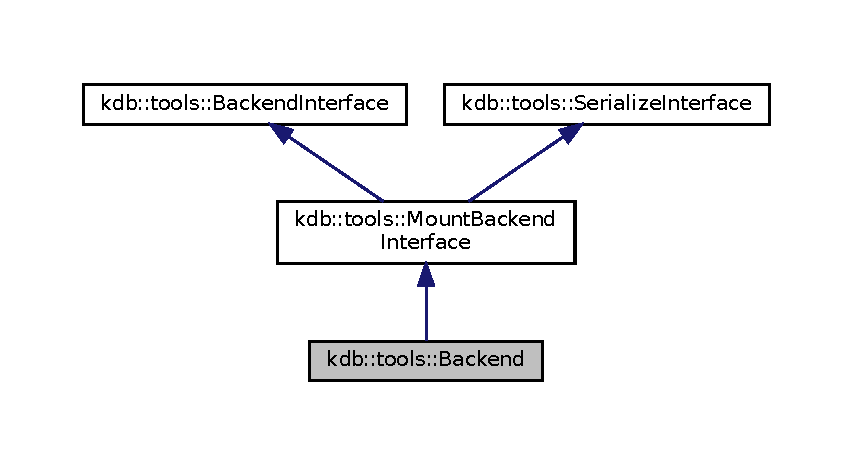
\includegraphics[width=350pt]{classkdb_1_1tools_1_1Backend__inherit__graph}
\end{center}
\end{figure}


Collaboration diagram for kdb\+::tools\+::Backend\+:
\nopagebreak
\begin{figure}[H]
\begin{center}
\leavevmode
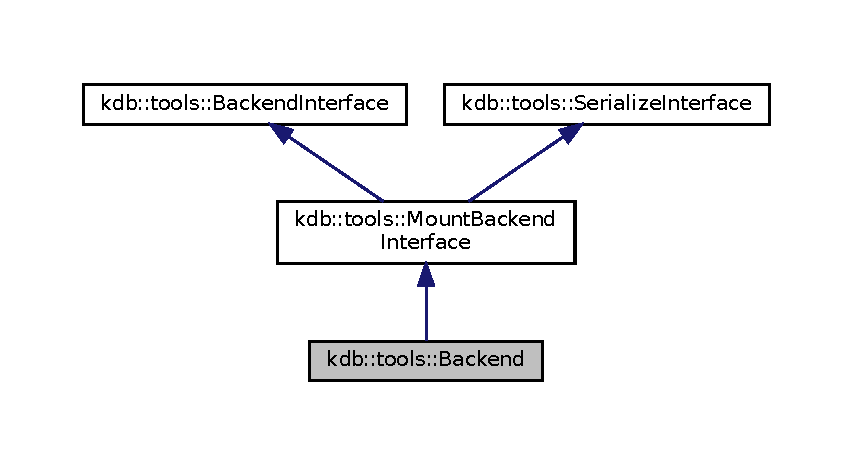
\includegraphics[width=350pt]{classkdb_1_1tools_1_1Backend__coll__graph}
\end{center}
\end{figure}
\doxysubsection*{Public Member Functions}
\begin{DoxyCompactItemize}
\item 
\mbox{\Hypertarget{classkdb_1_1tools_1_1Backend_a1650b149ebf313ee8cd3472247212263}\label{classkdb_1_1tools_1_1Backend_a1650b149ebf313ee8cd3472247212263}} 
\mbox{\hyperlink{classkdb_1_1tools_1_1Backend_a1650b149ebf313ee8cd3472247212263}{Backend}} ()
\begin{DoxyCompactList}\small\item\em Creates a new empty backend. \end{DoxyCompactList}\item 
void \mbox{\hyperlink{classkdb_1_1tools_1_1Backend_ac61b2628800a6fd0a6620ff47bfb3be9}{set\+Mountpoint}} (\mbox{\hyperlink{classkdb_1_1Key}{Key}} mountpoint, \mbox{\hyperlink{classkdb_1_1KeySet}{Key\+Set}} mount\+Conf)
\begin{DoxyCompactList}\small\item\em Sets the mountpoint for the backend. \end{DoxyCompactList}\item 
void \mbox{\hyperlink{classkdb_1_1tools_1_1Backend_aa7aa17a1c97cdfa48bcebadb7bc00247}{set\+Backend\+Config}} (\mbox{\hyperlink{classkdb_1_1KeySet}{Key\+Set}} const \&ks)
\begin{DoxyCompactList}\small\item\em \mbox{\hyperlink{classkdb_1_1tools_1_1Backend}{Backend}} Config to add to. \end{DoxyCompactList}\item 
void \mbox{\hyperlink{classkdb_1_1tools_1_1Backend_a2cce1cc51617baa5431a6036f5cfe05b}{add\+Plugin}} (\mbox{\hyperlink{classkdb_1_1tools_1_1PluginSpec}{Plugin\+Spec}} const \&spec)
\begin{DoxyCompactList}\small\item\em Add a plugin that can be loaded, meets all constraints. \end{DoxyCompactList}\item 
void \mbox{\hyperlink{classkdb_1_1tools_1_1Backend_a5c72747e5419d7802849cfc2eb4064d2}{use\+Config\+File}} (std\+::string file)
\item 
bool \mbox{\hyperlink{classkdb_1_1tools_1_1Backend_a7b28929231bc592c1a83f42121405496}{validated}} () const
\item 
void \mbox{\hyperlink{classkdb_1_1tools_1_1Backend_a93638ae12d8880bdb528ae709c857be7}{serialize}} (\mbox{\hyperlink{classkdb_1_1KeySet}{kdb\+::\+Key\+Set}} \&ret)
\end{DoxyCompactItemize}


\doxysubsection{Detailed Description}
A low-\/level representation of the backend (= set of plugins) that can be mounted. 

To build a backend, you should prefer \mbox{\hyperlink{classkdb_1_1tools_1_1BackendBuilder}{Backend\+Builder}}, which automatically fixes ordering and allows us to remove plugins. 

\doxysubsection{Member Function Documentation}
\mbox{\Hypertarget{classkdb_1_1tools_1_1Backend_a2cce1cc51617baa5431a6036f5cfe05b}\label{classkdb_1_1tools_1_1Backend_a2cce1cc51617baa5431a6036f5cfe05b}} 
\index{kdb::tools::Backend@{kdb::tools::Backend}!addPlugin@{addPlugin}}
\index{addPlugin@{addPlugin}!kdb::tools::Backend@{kdb::tools::Backend}}
\doxysubsubsection{\texorpdfstring{addPlugin()}{addPlugin()}}
{\footnotesize\ttfamily void kdb\+::tools\+::\+Backend\+::add\+Plugin (\begin{DoxyParamCaption}\item[{\mbox{\hyperlink{classkdb_1_1tools_1_1PluginSpec}{Plugin\+Spec}} const \&}]{plugin }\end{DoxyParamCaption})\hspace{0.3cm}{\ttfamily [virtual]}}



Add a plugin that can be loaded, meets all constraints. 

\begin{DoxyNote}{Note}
that this does not mean that the backend validates after it is added. It only means that the situation is not getting worse.
\end{DoxyNote}

\begin{DoxyExceptions}{Exceptions}
{\em Plugin\+Check\+Exception} & or its subclasses if it was not possible to load the plugin\\
\hline
\end{DoxyExceptions}
For validation \begin{DoxySeeAlso}{See also}
\mbox{\hyperlink{classkdb_1_1tools_1_1Backend_a7b28929231bc592c1a83f42121405496}{validated()}}. 
\end{DoxySeeAlso}


Implements \mbox{\hyperlink{classkdb_1_1tools_1_1BackendInterface}{kdb\+::tools\+::\+Backend\+Interface}}.

\mbox{\Hypertarget{classkdb_1_1tools_1_1Backend_a93638ae12d8880bdb528ae709c857be7}\label{classkdb_1_1tools_1_1Backend_a93638ae12d8880bdb528ae709c857be7}} 
\index{kdb::tools::Backend@{kdb::tools::Backend}!serialize@{serialize}}
\index{serialize@{serialize}!kdb::tools::Backend@{kdb::tools::Backend}}
\doxysubsubsection{\texorpdfstring{serialize()}{serialize()}}
{\footnotesize\ttfamily void kdb\+::tools\+::\+Backend\+::serialize (\begin{DoxyParamCaption}\item[{\mbox{\hyperlink{classkdb_1_1KeySet}{kdb\+::\+Key\+Set}} \&}]{ret }\end{DoxyParamCaption})\hspace{0.3cm}{\ttfamily [virtual]}}

\begin{DoxyPrecond}{Precondition}
name and mountpoint set Add plugin serialization into keyset ret.
\end{DoxyPrecond}
Only can be done once! (see first\+Ref in \mbox{\hyperlink{classkdb_1_1tools_1_1Plugin}{Plugin}}) 

Implements \mbox{\hyperlink{classkdb_1_1tools_1_1SerializeInterface}{kdb\+::tools\+::\+Serialize\+Interface}}.

\mbox{\Hypertarget{classkdb_1_1tools_1_1Backend_aa7aa17a1c97cdfa48bcebadb7bc00247}\label{classkdb_1_1tools_1_1Backend_aa7aa17a1c97cdfa48bcebadb7bc00247}} 
\index{kdb::tools::Backend@{kdb::tools::Backend}!setBackendConfig@{setBackendConfig}}
\index{setBackendConfig@{setBackendConfig}!kdb::tools::Backend@{kdb::tools::Backend}}
\doxysubsubsection{\texorpdfstring{setBackendConfig()}{setBackendConfig()}}
{\footnotesize\ttfamily void kdb\+::tools\+::\+Backend\+::set\+Backend\+Config (\begin{DoxyParamCaption}\item[{\mbox{\hyperlink{classkdb_1_1KeySet}{Key\+Set}} const \&}]{ks }\end{DoxyParamCaption})\hspace{0.3cm}{\ttfamily [virtual]}}



\mbox{\hyperlink{classkdb_1_1tools_1_1Backend}{Backend}} Config to add to. 


\begin{DoxyParams}{Parameters}
{\em ks} & the config to add, should be below system/ \\
\hline
\end{DoxyParams}


Implements \mbox{\hyperlink{classkdb_1_1tools_1_1MountBackendInterface}{kdb\+::tools\+::\+Mount\+Backend\+Interface}}.

\mbox{\Hypertarget{classkdb_1_1tools_1_1Backend_ac61b2628800a6fd0a6620ff47bfb3be9}\label{classkdb_1_1tools_1_1Backend_ac61b2628800a6fd0a6620ff47bfb3be9}} 
\index{kdb::tools::Backend@{kdb::tools::Backend}!setMountpoint@{setMountpoint}}
\index{setMountpoint@{setMountpoint}!kdb::tools::Backend@{kdb::tools::Backend}}
\doxysubsubsection{\texorpdfstring{setMountpoint()}{setMountpoint()}}
{\footnotesize\ttfamily void kdb\+::tools\+::\+Backend\+::set\+Mountpoint (\begin{DoxyParamCaption}\item[{\mbox{\hyperlink{classkdb_1_1Key}{Key}}}]{mountpoint,  }\item[{\mbox{\hyperlink{classkdb_1_1KeySet}{Key\+Set}}}]{mount\+Conf }\end{DoxyParamCaption})\hspace{0.3cm}{\ttfamily [virtual]}}



Sets the mountpoint for the backend. 


\begin{DoxyExceptions}{Exceptions}
{\em Mountpoint\+Invalid\+Exception} & \\
\hline
{\em Mountpoint\+Already\+In\+Use\+Exception} & \\
\hline
\end{DoxyExceptions}

\begin{DoxyParams}{Parameters}
{\em mountpoint} & the key name will be used as mountpoint. It is allowed to pass a key with a K\+E\+Y\+\_\+\+C\+A\+S\+C\+A\+D\+I\+N\+G\+\_\+\+N\+A\+ME\\
\hline
{\em mount\+Conf} & needs to include the keys below system/elektra/mountpoints \\
\hline
\end{DoxyParams}


Implements \mbox{\hyperlink{classkdb_1_1tools_1_1MountBackendInterface}{kdb\+::tools\+::\+Mount\+Backend\+Interface}}.

\mbox{\Hypertarget{classkdb_1_1tools_1_1Backend_a5c72747e5419d7802849cfc2eb4064d2}\label{classkdb_1_1tools_1_1Backend_a5c72747e5419d7802849cfc2eb4064d2}} 
\index{kdb::tools::Backend@{kdb::tools::Backend}!useConfigFile@{useConfigFile}}
\index{useConfigFile@{useConfigFile}!kdb::tools::Backend@{kdb::tools::Backend}}
\doxysubsubsection{\texorpdfstring{useConfigFile()}{useConfigFile()}}
{\footnotesize\ttfamily void kdb\+::tools\+::\+Backend\+::use\+Config\+File (\begin{DoxyParamCaption}\item[{std\+::string}]{file }\end{DoxyParamCaption})\hspace{0.3cm}{\ttfamily [virtual]}}

\begin{DoxyPrecond}{Precondition}
\+: resolver needs to be loaded first Will check the filename and use it as config\+File for this backend. 
\end{DoxyPrecond}

\begin{DoxyExceptions}{Exceptions}
{\em File\+Not\+Valid\+Exception} & if filename is not valid \\
\hline
{\em Missing\+Symbol} & if plugin does not implement \textquotesingle{}checkfile\textquotesingle{} \\
\hline
\end{DoxyExceptions}


Implements \mbox{\hyperlink{classkdb_1_1tools_1_1MountBackendInterface}{kdb\+::tools\+::\+Mount\+Backend\+Interface}}.

\mbox{\Hypertarget{classkdb_1_1tools_1_1Backend_a7b28929231bc592c1a83f42121405496}\label{classkdb_1_1tools_1_1Backend_a7b28929231bc592c1a83f42121405496}} 
\index{kdb::tools::Backend@{kdb::tools::Backend}!validated@{validated}}
\index{validated@{validated}!kdb::tools::Backend@{kdb::tools::Backend}}
\doxysubsubsection{\texorpdfstring{validated()}{validated()}}
{\footnotesize\ttfamily bool kdb\+::tools\+::\+Backend\+::validated (\begin{DoxyParamCaption}{ }\end{DoxyParamCaption}) const\hspace{0.3cm}{\ttfamily [virtual]}}

\begin{DoxyReturn}{Returns}
true if backend is validated 

false if more plugins are needed to be valided 
\end{DoxyReturn}


Implements \mbox{\hyperlink{classkdb_1_1tools_1_1MountBackendInterface}{kdb\+::tools\+::\+Mount\+Backend\+Interface}}.



The documentation for this class was generated from the following files\+:\begin{DoxyCompactItemize}
\item 
\mbox{\hyperlink{backend_8hpp}{backend.\+hpp}}\item 
\mbox{\hyperlink{src_2backend_8cpp}{src/backend.\+cpp}}\end{DoxyCompactItemize}

\hypertarget{structkdb_1_1tools_1_1BackendInfo}{}\doxysection{kdb\+::tools\+::Backend\+Info Struct Reference}
\label{structkdb_1_1tools_1_1BackendInfo}\index{kdb::tools::BackendInfo@{kdb::tools::BackendInfo}}


Info about a backend.  




{\ttfamily \#include $<$backends.\+hpp$>$}

\doxysubsection*{Public Attributes}
\begin{DoxyCompactItemize}
\item 
\mbox{\Hypertarget{structkdb_1_1tools_1_1BackendInfo_a7da85fc3a4bbb7412b0544aceeb9da75}\label{structkdb_1_1tools_1_1BackendInfo_a7da85fc3a4bbb7412b0544aceeb9da75}} 
std\+::string \mbox{\hyperlink{structkdb_1_1tools_1_1BackendInfo_a7da85fc3a4bbb7412b0544aceeb9da75}{name}}
\begin{DoxyCompactList}\small\item\em escaped mountpoint name (except for old mountpoints) \end{DoxyCompactList}\item 
\mbox{\Hypertarget{structkdb_1_1tools_1_1BackendInfo_a043c4414dc2b41bab37efb3c878f6cb8}\label{structkdb_1_1tools_1_1BackendInfo_a043c4414dc2b41bab37efb3c878f6cb8}} 
std\+::string \mbox{\hyperlink{structkdb_1_1tools_1_1BackendInfo_a043c4414dc2b41bab37efb3c878f6cb8}{mountpoint}}
\begin{DoxyCompactList}\small\item\em where the backend is mounted \end{DoxyCompactList}\item 
\mbox{\Hypertarget{structkdb_1_1tools_1_1BackendInfo_ac1d9984e01a78dba8e01dca0b91cbf30}\label{structkdb_1_1tools_1_1BackendInfo_ac1d9984e01a78dba8e01dca0b91cbf30}} 
std\+::string \mbox{\hyperlink{structkdb_1_1tools_1_1BackendInfo_ac1d9984e01a78dba8e01dca0b91cbf30}{path}}
\begin{DoxyCompactList}\small\item\em the configuration file path to this backend \end{DoxyCompactList}\end{DoxyCompactItemize}


\doxysubsection{Detailed Description}
Info about a backend. 

The documentation for this struct was generated from the following file\+:\begin{DoxyCompactItemize}
\item 
\mbox{\hyperlink{backends_8hpp}{backends.\+hpp}}\end{DoxyCompactItemize}

\hypertarget{classkdb_1_1tools_1_1Backends}{}\doxysection{kdb\+::tools\+::Backends Class Reference}
\label{classkdb_1_1tools_1_1Backends}\index{kdb::tools::Backends@{kdb::tools::Backends}}


Allows one to list backends.  




{\ttfamily \#include $<$backends.\+hpp$>$}

\doxysubsection*{Static Public Member Functions}
\begin{DoxyCompactItemize}
\item 
static Backend\+Info\+Vector \mbox{\hyperlink{classkdb_1_1tools_1_1Backends_a82b334d8a1e01df664462c6dd43bd7e1}{get\+Backend\+Info}} (\mbox{\hyperlink{classkdb_1_1KeySet}{Key\+Set}} mount\+Conf)
\begin{DoxyCompactList}\small\item\em give info about current mounted backends \end{DoxyCompactList}\item 
static \mbox{\hyperlink{structkdb_1_1tools_1_1BackendInfo}{Backend\+Info}} \mbox{\hyperlink{classkdb_1_1tools_1_1Backends_a692f3f6b5f01ed2e497a6e093e1e2e90}{find\+Backend}} (std\+::string const \&backend, \mbox{\hyperlink{classkdb_1_1KeySet}{Key\+Set}} mount\+Conf, bool verbose=false)
\begin{DoxyCompactList}\small\item\em Find a backend in the given name. \end{DoxyCompactList}\item 
static bool \mbox{\hyperlink{classkdb_1_1tools_1_1Backends_aca36f903059e3df0f2ded569d6d8df8c}{umount}} (std\+::string const \&backend, \mbox{\hyperlink{classkdb_1_1KeySet}{Key\+Set}} \&mount\+Conf)
\begin{DoxyCompactList}\small\item\em Unmount a backend by given mount\+Path. \end{DoxyCompactList}\item 
static std\+::string \mbox{\hyperlink{classkdb_1_1tools_1_1Backends_a76af9122c56426f4d0119e44719c7309}{get\+Base\+Path}} (std\+::string name)
\begin{DoxyCompactList}\small\item\em returns the base path of a mounted backend below system/elektra/mountpoints \end{DoxyCompactList}\end{DoxyCompactItemize}
\doxysubsection*{Static Public Attributes}
\begin{DoxyCompactItemize}
\item 
\mbox{\Hypertarget{classkdb_1_1tools_1_1Backends_ac867850accaab4fda286f763cacc3926}\label{classkdb_1_1tools_1_1Backends_ac867850accaab4fda286f763cacc3926}} 
static const char $\ast$ \mbox{\hyperlink{classkdb_1_1tools_1_1Backends_ac867850accaab4fda286f763cacc3926}{mountpoints\+Path}} = \char`\"{}system/elektra/mountpoints\char`\"{}
\begin{DoxyCompactList}\small\item\em Below this path is the mount\+Conf. \end{DoxyCompactList}\end{DoxyCompactItemize}


\doxysubsection{Detailed Description}
Allows one to list backends. 

\doxysubsection{Member Function Documentation}
\mbox{\Hypertarget{classkdb_1_1tools_1_1Backends_a692f3f6b5f01ed2e497a6e093e1e2e90}\label{classkdb_1_1tools_1_1Backends_a692f3f6b5f01ed2e497a6e093e1e2e90}} 
\index{kdb::tools::Backends@{kdb::tools::Backends}!findBackend@{findBackend}}
\index{findBackend@{findBackend}!kdb::tools::Backends@{kdb::tools::Backends}}
\doxysubsubsection{\texorpdfstring{findBackend()}{findBackend()}}
{\footnotesize\ttfamily \mbox{\hyperlink{structkdb_1_1tools_1_1BackendInfo}{Backend\+Info}} kdb\+::tools\+::\+Backends\+::find\+Backend (\begin{DoxyParamCaption}\item[{std\+::string const \&}]{mount\+Path,  }\item[{\mbox{\hyperlink{classkdb_1_1KeySet}{Key\+Set}}}]{mount\+Conf,  }\item[{bool}]{verbose = {\ttfamily false} }\end{DoxyParamCaption})\hspace{0.3cm}{\ttfamily [static]}}



Find a backend in the given name. 


\begin{DoxyParams}{Parameters}
{\em mount\+Path} & the given backend name to find\\
\hline
\end{DoxyParams}
For backwards compatibility old-\/style names containing \+\_\+ instead of escaped / are accepted if no modern-\/style mountpoint is found.


\begin{DoxyParams}{Parameters}
{\em mount\+Conf} & the configuration to search (should contain keys below mountpoints\+Path to find something)\\
\hline
\end{DoxyParams}
\begin{DoxyReturn}{Returns}
the found backend or an empty \mbox{\hyperlink{structkdb_1_1tools_1_1BackendInfo}{Backend\+Info}} if nothing found (with empty strings) 
\end{DoxyReturn}
\mbox{\Hypertarget{classkdb_1_1tools_1_1Backends_a82b334d8a1e01df664462c6dd43bd7e1}\label{classkdb_1_1tools_1_1Backends_a82b334d8a1e01df664462c6dd43bd7e1}} 
\index{kdb::tools::Backends@{kdb::tools::Backends}!getBackendInfo@{getBackendInfo}}
\index{getBackendInfo@{getBackendInfo}!kdb::tools::Backends@{kdb::tools::Backends}}
\doxysubsubsection{\texorpdfstring{getBackendInfo()}{getBackendInfo()}}
{\footnotesize\ttfamily Backends\+::\+Backend\+Info\+Vector kdb\+::tools\+::\+Backends\+::get\+Backend\+Info (\begin{DoxyParamCaption}\item[{\mbox{\hyperlink{classkdb_1_1KeySet}{Key\+Set}}}]{mount\+Conf }\end{DoxyParamCaption})\hspace{0.3cm}{\ttfamily [static]}}



give info about current mounted backends 


\begin{DoxyParams}{Parameters}
{\em mount\+Conf} & a keyset that contains everything below \mbox{\hyperlink{classkdb_1_1tools_1_1Backends_ac867850accaab4fda286f763cacc3926}{Backends\+::mountpoints\+Path}}\\
\hline
\end{DoxyParams}
\begin{DoxyReturn}{Returns}
an vector of information about mounted backends 
\end{DoxyReturn}
\mbox{\Hypertarget{classkdb_1_1tools_1_1Backends_a76af9122c56426f4d0119e44719c7309}\label{classkdb_1_1tools_1_1Backends_a76af9122c56426f4d0119e44719c7309}} 
\index{kdb::tools::Backends@{kdb::tools::Backends}!getBasePath@{getBasePath}}
\index{getBasePath@{getBasePath}!kdb::tools::Backends@{kdb::tools::Backends}}
\doxysubsubsection{\texorpdfstring{getBasePath()}{getBasePath()}}
{\footnotesize\ttfamily std\+::string kdb\+::tools\+::\+Backends\+::get\+Base\+Path (\begin{DoxyParamCaption}\item[{std\+::string}]{mp }\end{DoxyParamCaption})\hspace{0.3cm}{\ttfamily [static]}}



returns the base path of a mounted backend below system/elektra/mountpoints 


\begin{DoxyParams}{Parameters}
{\em mp} & the mountpoint (name will be derived from it)\\
\hline
\end{DoxyParams}
\begin{DoxyReturn}{Returns}
the properly prefixed and escaped name 
\end{DoxyReturn}
\mbox{\Hypertarget{classkdb_1_1tools_1_1Backends_aca36f903059e3df0f2ded569d6d8df8c}\label{classkdb_1_1tools_1_1Backends_aca36f903059e3df0f2ded569d6d8df8c}} 
\index{kdb::tools::Backends@{kdb::tools::Backends}!umount@{umount}}
\index{umount@{umount}!kdb::tools::Backends@{kdb::tools::Backends}}
\doxysubsubsection{\texorpdfstring{umount()}{umount()}}
{\footnotesize\ttfamily bool kdb\+::tools\+::\+Backends\+::umount (\begin{DoxyParamCaption}\item[{std\+::string const \&}]{mount\+Path,  }\item[{\mbox{\hyperlink{classkdb_1_1KeySet}{Key\+Set}} \&}]{mount\+Conf }\end{DoxyParamCaption})\hspace{0.3cm}{\ttfamily [static]}}



Unmount a backend by given mount\+Path. 


\begin{DoxyParams}{Parameters}
{\em mount\+Path} & the given mountpoint\\
\hline
\end{DoxyParams}
Uses \mbox{\hyperlink{classkdb_1_1tools_1_1Backends_a692f3f6b5f01ed2e497a6e093e1e2e90}{find\+Backend()}} to locate the backend.


\begin{DoxyRetVals}{Return values}
{\em true} & if something was done \\
\hline
{\em false} & if nothing was done (but also no error) \\
\hline
\end{DoxyRetVals}


The documentation for this class was generated from the following files\+:\begin{DoxyCompactItemize}
\item 
\mbox{\hyperlink{backends_8hpp}{backends.\+hpp}}\item 
\mbox{\hyperlink{backends_8cpp}{backends.\+cpp}}\end{DoxyCompactItemize}

\hypertarget{classkdb_1_1Context}{\section{kdb\-:\-:Context Class Reference}
\label{classkdb_1_1Context}\index{kdb\-::\-Context@{kdb\-::\-Context}}
}


Provides a context for configuration.  




{\ttfamily \#include $<$contextual.\-hpp$>$}



Inherits kdb\-::\-Subject.

\subsection*{Public Member Functions}
\begin{DoxyCompactItemize}
\item 
std\-::string \hyperlink{classkdb_1_1Context_a331463d2eec8d2a5fdb8ffe4bfc181f6}{operator\mbox{[}$\,$\mbox{]}} (std\-::string const \&layer) const 
\item 
void \hyperlink{classkdb_1_1Context_aa9ecaf4d6c47dee9ec20d490d09484db}{attach\-By\-Name} (std\-::string const \&key\-\_\-name, Observer \&observer)
\item 
std\-::string \hyperlink{classkdb_1_1Context_a130675fbe20f1b20eaa462ec6a9fe98e}{evaluate} (std\-::string const \&key\-\_\-name) const 
\item 
std\-::string \hyperlink{classkdb_1_1Context_a0687e0df9fbb3e2670fb45f1f9afdfc9}{evaluate} (std\-::string const \&key\-\_\-name, std\-::function$<$ bool(std\-::string const \&, std\-::string \&, bool in\-\_\-group)$>$ const \&on\-\_\-layer) const 
\item 
{\footnotesize template$<$typename T , typename... Args$>$ }\\void \hyperlink{classkdb_1_1Context_a592a5e238bfa36820c561d9dfc0bb8ee}{activate} (Args \&\&...args)
\begin{DoxyCompactList}\small\item\em Globally activate the layer. \end{DoxyCompactList}\end{DoxyCompactItemize}


\subsection{Detailed Description}
Provides a context for configuration. 

Is a subject for observers.

Holds currently active layers and allows global/scoped activation of layers. 

\subsection{Member Function Documentation}
\hypertarget{classkdb_1_1Context_a592a5e238bfa36820c561d9dfc0bb8ee}{\index{kdb\-::\-Context@{kdb\-::\-Context}!activate@{activate}}
\index{activate@{activate}!kdb::Context@{kdb\-::\-Context}}
\subsubsection[{activate}]{\setlength{\rightskip}{0pt plus 5cm}template$<$typename T , typename... Args$>$ void kdb\-::\-Context\-::activate (
\begin{DoxyParamCaption}
\item[{Args \&\&...}]{args}
\end{DoxyParamCaption}
)\hspace{0.3cm}{\ttfamily [inline]}}}\label{classkdb_1_1Context_a592a5e238bfa36820c561d9dfc0bb8ee}


Globally activate the layer. 


\begin{DoxyTemplParams}{Template Parameters}
{\em T} & the layer to activate \\
\hline
{\em Args} & the types for the arguments to pass to layer construction \\
\hline
\end{DoxyTemplParams}

\begin{DoxyParams}{Parameters}
{\em args} & the arguments to pass to layer construction \\
\hline
\end{DoxyParams}
\hypertarget{classkdb_1_1Context_aa9ecaf4d6c47dee9ec20d490d09484db}{\index{kdb\-::\-Context@{kdb\-::\-Context}!attach\-By\-Name@{attach\-By\-Name}}
\index{attach\-By\-Name@{attach\-By\-Name}!kdb::Context@{kdb\-::\-Context}}
\subsubsection[{attach\-By\-Name}]{\setlength{\rightskip}{0pt plus 5cm}void kdb\-::\-Context\-::attach\-By\-Name (
\begin{DoxyParamCaption}
\item[{std\-::string const \&}]{key\-\_\-name, }
\item[{Observer \&}]{observer}
\end{DoxyParamCaption}
)\hspace{0.3cm}{\ttfamily [inline]}}}\label{classkdb_1_1Context_aa9ecaf4d6c47dee9ec20d490d09484db}
Attach observer using to all events given by its specification (name)


\begin{DoxyParams}{Parameters}
{\em key\-\_\-name} & the name with placeholders to be used for attaching \\
\hline
{\em observer} & the observer to attach to \\
\hline
\end{DoxyParams}
\hypertarget{classkdb_1_1Context_a130675fbe20f1b20eaa462ec6a9fe98e}{\index{kdb\-::\-Context@{kdb\-::\-Context}!evaluate@{evaluate}}
\index{evaluate@{evaluate}!kdb::Context@{kdb\-::\-Context}}
\subsubsection[{evaluate}]{\setlength{\rightskip}{0pt plus 5cm}std\-::string kdb\-::\-Context\-::evaluate (
\begin{DoxyParamCaption}
\item[{std\-::string const \&}]{key\-\_\-name}
\end{DoxyParamCaption}
) const\hspace{0.3cm}{\ttfamily [inline]}}}\label{classkdb_1_1Context_a130675fbe20f1b20eaa462ec6a9fe98e}
Evaluate a specification (name) and return a key name under current context


\begin{DoxyParams}{Parameters}
{\em key\-\_\-name} & the name with placeholders to be evaluated \\
\hline
\end{DoxyParams}
\hypertarget{classkdb_1_1Context_a0687e0df9fbb3e2670fb45f1f9afdfc9}{\index{kdb\-::\-Context@{kdb\-::\-Context}!evaluate@{evaluate}}
\index{evaluate@{evaluate}!kdb::Context@{kdb\-::\-Context}}
\subsubsection[{evaluate}]{\setlength{\rightskip}{0pt plus 5cm}std\-::string kdb\-::\-Context\-::evaluate (
\begin{DoxyParamCaption}
\item[{std\-::string const \&}]{key\-\_\-name, }
\item[{std\-::function$<$ bool(std\-::string const \&, std\-::string \&, bool in\-\_\-group)$>$ const \&}]{on\-\_\-layer}
\end{DoxyParamCaption}
) const\hspace{0.3cm}{\ttfamily [inline]}}}\label{classkdb_1_1Context_a0687e0df9fbb3e2670fb45f1f9afdfc9}
Evaluate specification with this context.


\begin{DoxyParams}{Parameters}
{\em key\-\_\-name} & the keyname with placeholders to evaluate \\
\hline
{\em on\-\_\-layer} & the function to be called for every placeholder found\\
\hline
\end{DoxyParams}
\begin{DoxyParagraph}{on\-\_\-layer is called for every layer in the}
specification. 
\end{DoxyParagraph}
\hypertarget{classkdb_1_1Context_a331463d2eec8d2a5fdb8ffe4bfc181f6}{\index{kdb\-::\-Context@{kdb\-::\-Context}!operator\mbox{[}$\,$\mbox{]}@{operator[]}}
\index{operator\mbox{[}$\,$\mbox{]}@{operator[]}!kdb::Context@{kdb\-::\-Context}}
\subsubsection[{operator[]}]{\setlength{\rightskip}{0pt plus 5cm}std\-::string kdb\-::\-Context\-::operator\mbox{[}$\,$\mbox{]} (
\begin{DoxyParamCaption}
\item[{std\-::string const \&}]{layer}
\end{DoxyParamCaption}
) const\hspace{0.3cm}{\ttfamily [inline]}}}\label{classkdb_1_1Context_a331463d2eec8d2a5fdb8ffe4bfc181f6}
Lookup value for a current active layer


\begin{DoxyParams}{Parameters}
{\em layer} & the name of the requested layer \\
\hline
\end{DoxyParams}


The documentation for this class was generated from the following file\-:\begin{DoxyCompactItemize}
\item 
contextual.\-hpp\end{DoxyCompactItemize}

\hypertarget{classkdb_1_1KDB}{}\doxysection{kdb\+::KDB Class Reference}
\label{classkdb_1_1KDB}\index{kdb::KDB@{kdb::KDB}}


Constructs a class \mbox{\hyperlink{classkdb_1_1KDB}{KDB}}.  




{\ttfamily \#include $<$kdb.\+hpp$>$}



Inheritance diagram for kdb\+::KDB\+:
\nopagebreak
\begin{figure}[H]
\begin{center}
\leavevmode
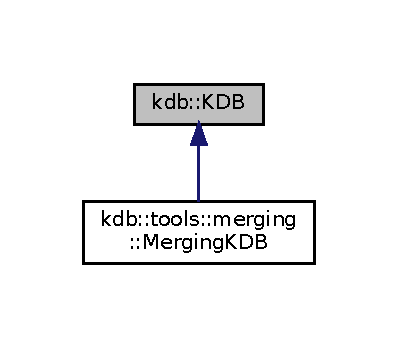
\includegraphics[width=191pt]{classkdb_1_1KDB__inherit__graph}
\end{center}
\end{figure}
\doxysubsection*{Public Member Functions}
\begin{DoxyCompactItemize}
\item 
\mbox{\hyperlink{classkdb_1_1KDB_a7e0637995ce9f294cdbc6f167df6db40}{KDB}} ()
\begin{DoxyCompactList}\small\item\em Constructs a class \mbox{\hyperlink{classkdb_1_1KDB}{KDB}}. \end{DoxyCompactList}\item 
\mbox{\hyperlink{classkdb_1_1KDB_a98e25c7fe2f47c5a90461676c6d219e7}{KDB}} (\mbox{\hyperlink{classkdb_1_1Key}{Key}} \&error\+Key)
\begin{DoxyCompactList}\small\item\em Constructs a class \mbox{\hyperlink{classkdb_1_1KDB}{KDB}}. \end{DoxyCompactList}\item 
\mbox{\hyperlink{classkdb_1_1KDB_adecb001cb936bd869ef06c7c71fdf0ef}{KDB}} (\mbox{\hyperlink{classkdb_1_1KeySet}{Key\+Set}} \&contract)
\begin{DoxyCompactList}\small\item\em Constructs a class \mbox{\hyperlink{classkdb_1_1KDB}{KDB}}. \end{DoxyCompactList}\item 
\mbox{\hyperlink{classkdb_1_1KDB_a95ef4570ac2d7ddbe2b4c0ad7810c742}{KDB}} (\mbox{\hyperlink{classkdb_1_1KeySet}{Key\+Set}} \&contract, \mbox{\hyperlink{classkdb_1_1Key}{Key}} \&error\+Key)
\begin{DoxyCompactList}\small\item\em Constructs a class \mbox{\hyperlink{classkdb_1_1KDB}{KDB}}. \end{DoxyCompactList}\item 
virtual void \mbox{\hyperlink{classkdb_1_1KDB_aee37484b06164eacc0cc11b7b40ab892}{open}} (\mbox{\hyperlink{classkdb_1_1Key}{Key}} \&error\+Key)
\begin{DoxyCompactList}\small\item\em Open the database. \end{DoxyCompactList}\item 
virtual void \mbox{\hyperlink{classkdb_1_1KDB_a8bd17da51bd531a2726185e7bbf4ecf9}{open}} (\mbox{\hyperlink{classkdb_1_1KeySet}{Key\+Set}} \&contract, \mbox{\hyperlink{classkdb_1_1Key}{Key}} \&error\+Key)
\begin{DoxyCompactList}\small\item\em Open the database. \end{DoxyCompactList}\item 
virtual void \mbox{\hyperlink{classkdb_1_1KDB_a1b3ff4a68c2c935d67dce843bc4ad01b}{close}} ()  throw ()
\begin{DoxyCompactList}\small\item\em Close the database. \end{DoxyCompactList}\item 
virtual void \mbox{\hyperlink{classkdb_1_1KDB_aa027a8f798a2cfee11ff712eb204c35d}{close}} (\mbox{\hyperlink{classkdb_1_1Key}{Key}} \&error\+Key)  throw ()
\begin{DoxyCompactList}\small\item\em Close the database. \end{DoxyCompactList}\item 
virtual int \mbox{\hyperlink{classkdb_1_1KDB_a0419ffbc273c89756bc523b4223ec25a}{get}} (\mbox{\hyperlink{classkdb_1_1KeySet}{Key\+Set}} \&returned, std\+::string const \&keyname)
\begin{DoxyCompactList}\small\item\em Get all keys below keyname inside returned. \end{DoxyCompactList}\item 
virtual int \mbox{\hyperlink{classkdb_1_1KDB_a48770a7290699bf2b7529f3ab67e378f}{get}} (\mbox{\hyperlink{classkdb_1_1KeySet}{Key\+Set}} \&returned, \mbox{\hyperlink{classkdb_1_1Key}{Key}} \&parent\+Key)
\begin{DoxyCompactList}\small\item\em Get all keys below parent\+Key inside returned. \end{DoxyCompactList}\item 
virtual int \mbox{\hyperlink{classkdb_1_1KDB_a29087a6a1a7de334f4e5b62ffe5d6e6e}{set}} (\mbox{\hyperlink{classkdb_1_1KeySet}{Key\+Set}} \&returned, std\+::string const \&keyname)
\begin{DoxyCompactList}\small\item\em Set all keys below keyname. \end{DoxyCompactList}\item 
virtual int \mbox{\hyperlink{classkdb_1_1KDB_a62a4fafbe21d9519b31a7868aa05f3e3}{set}} (\mbox{\hyperlink{classkdb_1_1KeySet}{Key\+Set}} \&returned, \mbox{\hyperlink{classkdb_1_1Key}{Key}} \&parent\+Key)
\begin{DoxyCompactList}\small\item\em Set all keys below parent\+Key. \end{DoxyCompactList}\end{DoxyCompactItemize}


\doxysubsection{Detailed Description}
Constructs a class \mbox{\hyperlink{classkdb_1_1KDB}{KDB}}. 


\begin{DoxyExceptions}{Exceptions}
{\em KDBException} & if database could not be opened\\
\hline
\end{DoxyExceptions}
Opens the session with the \mbox{\hyperlink{classkdb_1_1Key}{Key}} database. \begin{DoxyPrecond}{Precondition}
error\+Key must be a valid key, e.\+g. created with \mbox{\hyperlink{group__key_gad23c65b44bf48d773759e1f9a4d43b89}{key\+New()}}
\end{DoxyPrecond}
You must always call this method before retrieving or committing any keys to the database. At the end of a program, after using the \mbox{\hyperlink{classkdb_1_1Key}{Key}} database (\mbox{\hyperlink{classkdb_1_1KDB}{KDB}}), you must not forget to call \mbox{\hyperlink{group__kdb_gadb54dc9fda17ee07deb9444df745c96f}{kdb\+Close()}} to free resources.

The method will bootstrap itself in the following way. The first step is to open the default backend. With it {\ttfamily system\+:/elektra/mountpoints} will be loaded and all needed libraries and mountpoints will be determined. Then the global plugins and global keyset data from the {\ttfamily contract} is processed. Finally, the libraries for backends will be loaded and with it the {\ttfamily \mbox{\hyperlink{classkdb_1_1KDB}{KDB}}} data structure will be initialized.

The pointer to the {\ttfamily \mbox{\hyperlink{classkdb_1_1KDB}{KDB}}} structure returned will be initialized like described above, and it must be passed along on any kdb$\ast$() method your application calls.

Get a {\ttfamily \mbox{\hyperlink{classkdb_1_1KDB}{KDB}}} handle for every thread using elektra. Don\textquotesingle{}t share the handle across threads, and also not the pointer accessing it\+:


\begin{DoxyCodeInclude}{0}
\DoxyCodeLine{\textcolor{keywordtype}{void} thread1 (\textcolor{keywordtype}{void})}
\DoxyCodeLine{\{}
\DoxyCodeLine{        Key * parent = \mbox{\hyperlink{group__key_gad23c65b44bf48d773759e1f9a4d43b89}{keyNew}} (\textcolor{stringliteral}{"{}/app/part1"{}}, \mbox{\hyperlink{group__key_gga9b703ca49f48b482def322b77d3e6bc8aa8adb6fcb92dec58fb19410eacfdd403}{KEY\_END}});}
\DoxyCodeLine{        \mbox{\hyperlink{classkdb_1_1KDB_a7e0637995ce9f294cdbc6f167df6db40}{KDB}} * h = \mbox{\hyperlink{group__kdb_ga844e1299a84c3fbf1d3a905c5c893ba5}{kdbOpen}} (NULL, parent);}
\DoxyCodeLine{        \textcolor{comment}{// fetch keys and work with them}}
\DoxyCodeLine{        \mbox{\hyperlink{group__kdb_gadb54dc9fda17ee07deb9444df745c96f}{kdbClose}} (h, parent);}
\DoxyCodeLine{\}}
\DoxyCodeLine{\textcolor{keywordtype}{void} thread2 (\textcolor{keywordtype}{void})}
\DoxyCodeLine{\{}
\DoxyCodeLine{        Key * parent = \mbox{\hyperlink{group__key_gad23c65b44bf48d773759e1f9a4d43b89}{keyNew}} (\textcolor{stringliteral}{"{}/app/part2"{}}, \mbox{\hyperlink{group__key_gga9b703ca49f48b482def322b77d3e6bc8aa8adb6fcb92dec58fb19410eacfdd403}{KEY\_END}});}
\DoxyCodeLine{        \mbox{\hyperlink{classkdb_1_1KDB_a7e0637995ce9f294cdbc6f167df6db40}{KDB}} * h = \mbox{\hyperlink{group__kdb_ga844e1299a84c3fbf1d3a905c5c893ba5}{kdbOpen}} (NULL, parent);}
\DoxyCodeLine{        \textcolor{comment}{// fetch keys and work with them}}
\DoxyCodeLine{        \mbox{\hyperlink{group__kdb_gadb54dc9fda17ee07deb9444df745c96f}{kdbClose}} (h, parent);}
\DoxyCodeLine{\}}

\end{DoxyCodeInclude}
 You don\textquotesingle{}t need \mbox{\hyperlink{group__kdb_ga844e1299a84c3fbf1d3a905c5c893ba5}{kdb\+Open()}} if you only want to manipulate plain in-\/memory \mbox{\hyperlink{classkdb_1_1Key}{Key}} or \mbox{\hyperlink{classkdb_1_1KeySet}{Key\+Set}} objects.

\begin{DoxyPrecond}{Precondition}
error\+Key must be a valid key, e.\+g. created with \mbox{\hyperlink{group__key_gad23c65b44bf48d773759e1f9a4d43b89}{key\+New()}}
\end{DoxyPrecond}

\begin{DoxyParams}{Parameters}
{\em contract} & the contract that should be ensured before opening the \mbox{\hyperlink{classkdb_1_1KDB}{KDB}} all data is copied and the \mbox{\hyperlink{classkdb_1_1KeySet}{Key\+Set}} can safely be used for e.\+g. \mbox{\hyperlink{group__kdb_ga28e385fd9cb7ccfe0b2f1ed2f62453a1}{kdb\+Get()}} later \\
\hline
{\em error\+Key} & the key which holds errors and warnings which were issued\\
\hline
\end{DoxyParams}
\begin{DoxyReturn}{Returns}
handle to the newly created \mbox{\hyperlink{classkdb_1_1KDB}{KDB}} on success 
\end{DoxyReturn}

\begin{DoxyRetVals}{Return values}
{\em NULL} & on failure\\
\hline
\end{DoxyRetVals}
\begin{DoxySince}{Since}
1.\+0.\+0
\end{DoxySince}
\begin{DoxySeeAlso}{See also}
\mbox{\hyperlink{group__kdb_gadb54dc9fda17ee07deb9444df745c96f}{kdb\+Close()}} to \mbox{\hyperlink{classkdb_1_1KDB_a1b3ff4a68c2c935d67dce843bc4ad01b}{close}} the session of a \mbox{\hyperlink{classkdb_1_1Key}{Key}} database opened by \mbox{\hyperlink{group__kdb_ga844e1299a84c3fbf1d3a905c5c893ba5}{kdb\+Open()}}
\end{DoxySeeAlso}
Access to the key database.

\begin{DoxyInvariant}{Invariant}
the object holds a valid connection to the key database or is empty 
\end{DoxyInvariant}


\doxysubsection{Constructor \& Destructor Documentation}
\mbox{\Hypertarget{classkdb_1_1KDB_a7e0637995ce9f294cdbc6f167df6db40}\label{classkdb_1_1KDB_a7e0637995ce9f294cdbc6f167df6db40}} 
\index{kdb::KDB@{kdb::KDB}!KDB@{KDB}}
\index{KDB@{KDB}!kdb::KDB@{kdb::KDB}}
\doxysubsubsection{\texorpdfstring{KDB()}{KDB()}\hspace{0.1cm}{\footnotesize\ttfamily [1/4]}}
{\footnotesize\ttfamily kdb\+::\+KDB\+::\+KDB (\begin{DoxyParamCaption}{ }\end{DoxyParamCaption})\hspace{0.3cm}{\ttfamily [inline]}}



Constructs a class \mbox{\hyperlink{classkdb_1_1KDB}{KDB}}. 


\begin{DoxyExceptions}{Exceptions}
{\em KDBException} & if database could not be opened\\
\hline
\end{DoxyExceptions}
Opens the session with the \mbox{\hyperlink{classkdb_1_1Key}{Key}} database. \begin{DoxyPrecond}{Precondition}
error\+Key must be a valid key, e.\+g. created with \mbox{\hyperlink{group__key_gad23c65b44bf48d773759e1f9a4d43b89}{key\+New()}}
\end{DoxyPrecond}
You must always call this method before retrieving or committing any keys to the database. At the end of a program, after using the \mbox{\hyperlink{classkdb_1_1Key}{Key}} database (\mbox{\hyperlink{classkdb_1_1KDB}{KDB}}), you must not forget to call \mbox{\hyperlink{group__kdb_gadb54dc9fda17ee07deb9444df745c96f}{kdb\+Close()}} to free resources.

The method will bootstrap itself in the following way. The first step is to open the default backend. With it {\ttfamily system\+:/elektra/mountpoints} will be loaded and all needed libraries and mountpoints will be determined. Then the global plugins and global keyset data from the {\ttfamily contract} is processed. Finally, the libraries for backends will be loaded and with it the {\ttfamily \mbox{\hyperlink{classkdb_1_1KDB}{KDB}}} data structure will be initialized.

The pointer to the {\ttfamily \mbox{\hyperlink{classkdb_1_1KDB}{KDB}}} structure returned will be initialized like described above, and it must be passed along on any kdb$\ast$() method your application calls.

Get a {\ttfamily \mbox{\hyperlink{classkdb_1_1KDB}{KDB}}} handle for every thread using elektra. Don\textquotesingle{}t share the handle across threads, and also not the pointer accessing it\+:


\begin{DoxyCodeInclude}{0}
\DoxyCodeLine{\textcolor{keywordtype}{void} thread1 (\textcolor{keywordtype}{void})}
\DoxyCodeLine{\{}
\DoxyCodeLine{        Key * parent = \mbox{\hyperlink{group__key_gad23c65b44bf48d773759e1f9a4d43b89}{keyNew}} (\textcolor{stringliteral}{"{}/app/part1"{}}, \mbox{\hyperlink{group__key_gga9b703ca49f48b482def322b77d3e6bc8aa8adb6fcb92dec58fb19410eacfdd403}{KEY\_END}});}
\DoxyCodeLine{        \mbox{\hyperlink{classkdb_1_1KDB_a7e0637995ce9f294cdbc6f167df6db40}{KDB}} * h = \mbox{\hyperlink{group__kdb_ga844e1299a84c3fbf1d3a905c5c893ba5}{kdbOpen}} (NULL, parent);}
\DoxyCodeLine{        \textcolor{comment}{// fetch keys and work with them}}
\DoxyCodeLine{        \mbox{\hyperlink{group__kdb_gadb54dc9fda17ee07deb9444df745c96f}{kdbClose}} (h, parent);}
\DoxyCodeLine{\}}
\DoxyCodeLine{\textcolor{keywordtype}{void} thread2 (\textcolor{keywordtype}{void})}
\DoxyCodeLine{\{}
\DoxyCodeLine{        Key * parent = \mbox{\hyperlink{group__key_gad23c65b44bf48d773759e1f9a4d43b89}{keyNew}} (\textcolor{stringliteral}{"{}/app/part2"{}}, \mbox{\hyperlink{group__key_gga9b703ca49f48b482def322b77d3e6bc8aa8adb6fcb92dec58fb19410eacfdd403}{KEY\_END}});}
\DoxyCodeLine{        \mbox{\hyperlink{classkdb_1_1KDB_a7e0637995ce9f294cdbc6f167df6db40}{KDB}} * h = \mbox{\hyperlink{group__kdb_ga844e1299a84c3fbf1d3a905c5c893ba5}{kdbOpen}} (NULL, parent);}
\DoxyCodeLine{        \textcolor{comment}{// fetch keys and work with them}}
\DoxyCodeLine{        \mbox{\hyperlink{group__kdb_gadb54dc9fda17ee07deb9444df745c96f}{kdbClose}} (h, parent);}
\DoxyCodeLine{\}}

\end{DoxyCodeInclude}
 You don\textquotesingle{}t need \mbox{\hyperlink{group__kdb_ga844e1299a84c3fbf1d3a905c5c893ba5}{kdb\+Open()}} if you only want to manipulate plain in-\/memory \mbox{\hyperlink{classkdb_1_1Key}{Key}} or \mbox{\hyperlink{classkdb_1_1KeySet}{Key\+Set}} objects.

\begin{DoxyPrecond}{Precondition}
error\+Key must be a valid key, e.\+g. created with \mbox{\hyperlink{group__key_gad23c65b44bf48d773759e1f9a4d43b89}{key\+New()}}
\end{DoxyPrecond}

\begin{DoxyParams}{Parameters}
{\em contract} & the contract that should be ensured before opening the \mbox{\hyperlink{classkdb_1_1KDB}{KDB}} all data is copied and the \mbox{\hyperlink{classkdb_1_1KeySet}{Key\+Set}} can safely be used for e.\+g. \mbox{\hyperlink{group__kdb_ga28e385fd9cb7ccfe0b2f1ed2f62453a1}{kdb\+Get()}} later \\
\hline
{\em error\+Key} & the key which holds errors and warnings which were issued\\
\hline
\end{DoxyParams}
\begin{DoxyReturn}{Returns}
handle to the newly created \mbox{\hyperlink{classkdb_1_1KDB}{KDB}} on success 
\end{DoxyReturn}

\begin{DoxyRetVals}{Return values}
{\em NULL} & on failure\\
\hline
\end{DoxyRetVals}
\begin{DoxySince}{Since}
1.\+0.\+0
\end{DoxySince}
\begin{DoxySeeAlso}{See also}
\mbox{\hyperlink{group__kdb_gadb54dc9fda17ee07deb9444df745c96f}{kdb\+Close()}} to \mbox{\hyperlink{classkdb_1_1KDB_a1b3ff4a68c2c935d67dce843bc4ad01b}{close}} the session of a \mbox{\hyperlink{classkdb_1_1Key}{Key}} database opened by \mbox{\hyperlink{group__kdb_ga844e1299a84c3fbf1d3a905c5c893ba5}{kdb\+Open()}} 
\end{DoxySeeAlso}
\mbox{\Hypertarget{classkdb_1_1KDB_a98e25c7fe2f47c5a90461676c6d219e7}\label{classkdb_1_1KDB_a98e25c7fe2f47c5a90461676c6d219e7}} 
\index{kdb::KDB@{kdb::KDB}!KDB@{KDB}}
\index{KDB@{KDB}!kdb::KDB@{kdb::KDB}}
\doxysubsubsection{\texorpdfstring{KDB()}{KDB()}\hspace{0.1cm}{\footnotesize\ttfamily [2/4]}}
{\footnotesize\ttfamily kdb\+::\+KDB\+::\+KDB (\begin{DoxyParamCaption}\item[{\mbox{\hyperlink{classkdb_1_1Key}{Key}} \&}]{error\+Key }\end{DoxyParamCaption})\hspace{0.3cm}{\ttfamily [inline]}, {\ttfamily [explicit]}}



Constructs a class \mbox{\hyperlink{classkdb_1_1KDB}{KDB}}. 


\begin{DoxyParams}{Parameters}
{\em error\+Key} & is useful if you want to get the warnings in the successful case, when no exception is thrown.\\
\hline
\end{DoxyParams}

\begin{DoxyExceptions}{Exceptions}
{\em KDBException} & if database could not be opened\\
\hline
\end{DoxyExceptions}
Opens the session with the \mbox{\hyperlink{classkdb_1_1Key}{Key}} database. \begin{DoxyPrecond}{Precondition}
error\+Key must be a valid key, e.\+g. created with \mbox{\hyperlink{group__key_gad23c65b44bf48d773759e1f9a4d43b89}{key\+New()}}
\end{DoxyPrecond}
You must always call this method before retrieving or committing any keys to the database. At the end of a program, after using the \mbox{\hyperlink{classkdb_1_1Key}{Key}} database (\mbox{\hyperlink{classkdb_1_1KDB}{KDB}}), you must not forget to call \mbox{\hyperlink{group__kdb_gadb54dc9fda17ee07deb9444df745c96f}{kdb\+Close()}} to free resources.

The method will bootstrap itself in the following way. The first step is to open the default backend. With it {\ttfamily system\+:/elektra/mountpoints} will be loaded and all needed libraries and mountpoints will be determined. Then the global plugins and global keyset data from the {\ttfamily contract} is processed. Finally, the libraries for backends will be loaded and with it the {\ttfamily \mbox{\hyperlink{classkdb_1_1KDB}{KDB}}} data structure will be initialized.

The pointer to the {\ttfamily \mbox{\hyperlink{classkdb_1_1KDB}{KDB}}} structure returned will be initialized like described above, and it must be passed along on any kdb$\ast$() method your application calls.

Get a {\ttfamily \mbox{\hyperlink{classkdb_1_1KDB}{KDB}}} handle for every thread using elektra. Don\textquotesingle{}t share the handle across threads, and also not the pointer accessing it\+:


\begin{DoxyCodeInclude}{0}
\DoxyCodeLine{\textcolor{keywordtype}{void} thread1 (\textcolor{keywordtype}{void})}
\DoxyCodeLine{\{}
\DoxyCodeLine{        Key * parent = \mbox{\hyperlink{group__key_gad23c65b44bf48d773759e1f9a4d43b89}{keyNew}} (\textcolor{stringliteral}{"{}/app/part1"{}}, \mbox{\hyperlink{group__key_gga9b703ca49f48b482def322b77d3e6bc8aa8adb6fcb92dec58fb19410eacfdd403}{KEY\_END}});}
\DoxyCodeLine{        \mbox{\hyperlink{classkdb_1_1KDB_a7e0637995ce9f294cdbc6f167df6db40}{KDB}} * h = \mbox{\hyperlink{group__kdb_ga844e1299a84c3fbf1d3a905c5c893ba5}{kdbOpen}} (NULL, parent);}
\DoxyCodeLine{        \textcolor{comment}{// fetch keys and work with them}}
\DoxyCodeLine{        \mbox{\hyperlink{group__kdb_gadb54dc9fda17ee07deb9444df745c96f}{kdbClose}} (h, parent);}
\DoxyCodeLine{\}}
\DoxyCodeLine{\textcolor{keywordtype}{void} thread2 (\textcolor{keywordtype}{void})}
\DoxyCodeLine{\{}
\DoxyCodeLine{        Key * parent = \mbox{\hyperlink{group__key_gad23c65b44bf48d773759e1f9a4d43b89}{keyNew}} (\textcolor{stringliteral}{"{}/app/part2"{}}, \mbox{\hyperlink{group__key_gga9b703ca49f48b482def322b77d3e6bc8aa8adb6fcb92dec58fb19410eacfdd403}{KEY\_END}});}
\DoxyCodeLine{        \mbox{\hyperlink{classkdb_1_1KDB_a7e0637995ce9f294cdbc6f167df6db40}{KDB}} * h = \mbox{\hyperlink{group__kdb_ga844e1299a84c3fbf1d3a905c5c893ba5}{kdbOpen}} (NULL, parent);}
\DoxyCodeLine{        \textcolor{comment}{// fetch keys and work with them}}
\DoxyCodeLine{        \mbox{\hyperlink{group__kdb_gadb54dc9fda17ee07deb9444df745c96f}{kdbClose}} (h, parent);}
\DoxyCodeLine{\}}

\end{DoxyCodeInclude}
 You don\textquotesingle{}t need \mbox{\hyperlink{group__kdb_ga844e1299a84c3fbf1d3a905c5c893ba5}{kdb\+Open()}} if you only want to manipulate plain in-\/memory \mbox{\hyperlink{classkdb_1_1Key}{Key}} or \mbox{\hyperlink{classkdb_1_1KeySet}{Key\+Set}} objects.

\begin{DoxyPrecond}{Precondition}
error\+Key must be a valid key, e.\+g. created with \mbox{\hyperlink{group__key_gad23c65b44bf48d773759e1f9a4d43b89}{key\+New()}}
\end{DoxyPrecond}

\begin{DoxyParams}{Parameters}
{\em contract} & the contract that should be ensured before opening the \mbox{\hyperlink{classkdb_1_1KDB}{KDB}} all data is copied and the \mbox{\hyperlink{classkdb_1_1KeySet}{Key\+Set}} can safely be used for e.\+g. \mbox{\hyperlink{group__kdb_ga28e385fd9cb7ccfe0b2f1ed2f62453a1}{kdb\+Get()}} later \\
\hline
{\em error\+Key} & the key which holds errors and warnings which were issued\\
\hline
\end{DoxyParams}
\begin{DoxyReturn}{Returns}
handle to the newly created \mbox{\hyperlink{classkdb_1_1KDB}{KDB}} on success 
\end{DoxyReturn}

\begin{DoxyRetVals}{Return values}
{\em NULL} & on failure\\
\hline
\end{DoxyRetVals}
\begin{DoxySince}{Since}
1.\+0.\+0
\end{DoxySince}
\begin{DoxySeeAlso}{See also}
\mbox{\hyperlink{group__kdb_gadb54dc9fda17ee07deb9444df745c96f}{kdb\+Close()}} to \mbox{\hyperlink{classkdb_1_1KDB_a1b3ff4a68c2c935d67dce843bc4ad01b}{close}} the session of a \mbox{\hyperlink{classkdb_1_1Key}{Key}} database opened by \mbox{\hyperlink{group__kdb_ga844e1299a84c3fbf1d3a905c5c893ba5}{kdb\+Open()}} 
\end{DoxySeeAlso}
\mbox{\Hypertarget{classkdb_1_1KDB_adecb001cb936bd869ef06c7c71fdf0ef}\label{classkdb_1_1KDB_adecb001cb936bd869ef06c7c71fdf0ef}} 
\index{kdb::KDB@{kdb::KDB}!KDB@{KDB}}
\index{KDB@{KDB}!kdb::KDB@{kdb::KDB}}
\doxysubsubsection{\texorpdfstring{KDB()}{KDB()}\hspace{0.1cm}{\footnotesize\ttfamily [3/4]}}
{\footnotesize\ttfamily kdb\+::\+KDB\+::\+KDB (\begin{DoxyParamCaption}\item[{\mbox{\hyperlink{classkdb_1_1KeySet}{Key\+Set}} \&}]{contract }\end{DoxyParamCaption})\hspace{0.3cm}{\ttfamily [inline]}, {\ttfamily [explicit]}}



Constructs a class \mbox{\hyperlink{classkdb_1_1KDB}{KDB}}. 


\begin{DoxyParams}{Parameters}
{\em contract} & the contract that should be ensured \\
\hline
{\em error\+Key} & is useful if you want to get the warnings in the successful case, when no exception is thrown.\\
\hline
\end{DoxyParams}

\begin{DoxyExceptions}{Exceptions}
{\em KDBException} & if database could not be opened\\
\hline
\end{DoxyExceptions}
Opens the session with the \mbox{\hyperlink{classkdb_1_1Key}{Key}} database. \begin{DoxyPrecond}{Precondition}
error\+Key must be a valid key, e.\+g. created with \mbox{\hyperlink{group__key_gad23c65b44bf48d773759e1f9a4d43b89}{key\+New()}}
\end{DoxyPrecond}
You must always call this method before retrieving or committing any keys to the database. At the end of a program, after using the \mbox{\hyperlink{classkdb_1_1Key}{Key}} database (\mbox{\hyperlink{classkdb_1_1KDB}{KDB}}), you must not forget to call \mbox{\hyperlink{group__kdb_gadb54dc9fda17ee07deb9444df745c96f}{kdb\+Close()}} to free resources.

The method will bootstrap itself in the following way. The first step is to open the default backend. With it {\ttfamily system\+:/elektra/mountpoints} will be loaded and all needed libraries and mountpoints will be determined. Then the global plugins and global keyset data from the {\ttfamily contract} is processed. Finally, the libraries for backends will be loaded and with it the {\ttfamily \mbox{\hyperlink{classkdb_1_1KDB}{KDB}}} data structure will be initialized.

The pointer to the {\ttfamily \mbox{\hyperlink{classkdb_1_1KDB}{KDB}}} structure returned will be initialized like described above, and it must be passed along on any kdb$\ast$() method your application calls.

Get a {\ttfamily \mbox{\hyperlink{classkdb_1_1KDB}{KDB}}} handle for every thread using elektra. Don\textquotesingle{}t share the handle across threads, and also not the pointer accessing it\+:


\begin{DoxyCodeInclude}{0}
\DoxyCodeLine{\textcolor{keywordtype}{void} thread1 (\textcolor{keywordtype}{void})}
\DoxyCodeLine{\{}
\DoxyCodeLine{        Key * parent = \mbox{\hyperlink{group__key_gad23c65b44bf48d773759e1f9a4d43b89}{keyNew}} (\textcolor{stringliteral}{"{}/app/part1"{}}, \mbox{\hyperlink{group__key_gga9b703ca49f48b482def322b77d3e6bc8aa8adb6fcb92dec58fb19410eacfdd403}{KEY\_END}});}
\DoxyCodeLine{        \mbox{\hyperlink{classkdb_1_1KDB_a7e0637995ce9f294cdbc6f167df6db40}{KDB}} * h = \mbox{\hyperlink{group__kdb_ga844e1299a84c3fbf1d3a905c5c893ba5}{kdbOpen}} (NULL, parent);}
\DoxyCodeLine{        \textcolor{comment}{// fetch keys and work with them}}
\DoxyCodeLine{        \mbox{\hyperlink{group__kdb_gadb54dc9fda17ee07deb9444df745c96f}{kdbClose}} (h, parent);}
\DoxyCodeLine{\}}
\DoxyCodeLine{\textcolor{keywordtype}{void} thread2 (\textcolor{keywordtype}{void})}
\DoxyCodeLine{\{}
\DoxyCodeLine{        Key * parent = \mbox{\hyperlink{group__key_gad23c65b44bf48d773759e1f9a4d43b89}{keyNew}} (\textcolor{stringliteral}{"{}/app/part2"{}}, \mbox{\hyperlink{group__key_gga9b703ca49f48b482def322b77d3e6bc8aa8adb6fcb92dec58fb19410eacfdd403}{KEY\_END}});}
\DoxyCodeLine{        \mbox{\hyperlink{classkdb_1_1KDB_a7e0637995ce9f294cdbc6f167df6db40}{KDB}} * h = \mbox{\hyperlink{group__kdb_ga844e1299a84c3fbf1d3a905c5c893ba5}{kdbOpen}} (NULL, parent);}
\DoxyCodeLine{        \textcolor{comment}{// fetch keys and work with them}}
\DoxyCodeLine{        \mbox{\hyperlink{group__kdb_gadb54dc9fda17ee07deb9444df745c96f}{kdbClose}} (h, parent);}
\DoxyCodeLine{\}}

\end{DoxyCodeInclude}
 You don\textquotesingle{}t need \mbox{\hyperlink{group__kdb_ga844e1299a84c3fbf1d3a905c5c893ba5}{kdb\+Open()}} if you only want to manipulate plain in-\/memory \mbox{\hyperlink{classkdb_1_1Key}{Key}} or \mbox{\hyperlink{classkdb_1_1KeySet}{Key\+Set}} objects.

\begin{DoxyPrecond}{Precondition}
error\+Key must be a valid key, e.\+g. created with \mbox{\hyperlink{group__key_gad23c65b44bf48d773759e1f9a4d43b89}{key\+New()}}
\end{DoxyPrecond}

\begin{DoxyParams}{Parameters}
{\em contract} & the contract that should be ensured before opening the \mbox{\hyperlink{classkdb_1_1KDB}{KDB}} all data is copied and the \mbox{\hyperlink{classkdb_1_1KeySet}{Key\+Set}} can safely be used for e.\+g. \mbox{\hyperlink{group__kdb_ga28e385fd9cb7ccfe0b2f1ed2f62453a1}{kdb\+Get()}} later \\
\hline
{\em error\+Key} & the key which holds errors and warnings which were issued\\
\hline
\end{DoxyParams}
\begin{DoxyReturn}{Returns}
handle to the newly created \mbox{\hyperlink{classkdb_1_1KDB}{KDB}} on success 
\end{DoxyReturn}

\begin{DoxyRetVals}{Return values}
{\em NULL} & on failure\\
\hline
\end{DoxyRetVals}
\begin{DoxySince}{Since}
1.\+0.\+0
\end{DoxySince}
\begin{DoxySeeAlso}{See also}
\mbox{\hyperlink{group__kdb_gadb54dc9fda17ee07deb9444df745c96f}{kdb\+Close()}} to \mbox{\hyperlink{classkdb_1_1KDB_a1b3ff4a68c2c935d67dce843bc4ad01b}{close}} the session of a \mbox{\hyperlink{classkdb_1_1Key}{Key}} database opened by \mbox{\hyperlink{group__kdb_ga844e1299a84c3fbf1d3a905c5c893ba5}{kdb\+Open()}} 
\end{DoxySeeAlso}
\mbox{\Hypertarget{classkdb_1_1KDB_a95ef4570ac2d7ddbe2b4c0ad7810c742}\label{classkdb_1_1KDB_a95ef4570ac2d7ddbe2b4c0ad7810c742}} 
\index{kdb::KDB@{kdb::KDB}!KDB@{KDB}}
\index{KDB@{KDB}!kdb::KDB@{kdb::KDB}}
\doxysubsubsection{\texorpdfstring{KDB()}{KDB()}\hspace{0.1cm}{\footnotesize\ttfamily [4/4]}}
{\footnotesize\ttfamily kdb\+::\+KDB\+::\+KDB (\begin{DoxyParamCaption}\item[{\mbox{\hyperlink{classkdb_1_1KeySet}{Key\+Set}} \&}]{contract,  }\item[{\mbox{\hyperlink{classkdb_1_1Key}{Key}} \&}]{error\+Key }\end{DoxyParamCaption})\hspace{0.3cm}{\ttfamily [inline]}}



Constructs a class \mbox{\hyperlink{classkdb_1_1KDB}{KDB}}. 


\begin{DoxyParams}{Parameters}
{\em contract} & the contract that should be ensured \\
\hline
{\em error\+Key} & is useful if you want to get the warnings in the successful case, when no exception is thrown.\\
\hline
\end{DoxyParams}

\begin{DoxyExceptions}{Exceptions}
{\em KDBException} & if database could not be opened\\
\hline
\end{DoxyExceptions}
Opens the session with the \mbox{\hyperlink{classkdb_1_1Key}{Key}} database. \begin{DoxyPrecond}{Precondition}
error\+Key must be a valid key, e.\+g. created with \mbox{\hyperlink{group__key_gad23c65b44bf48d773759e1f9a4d43b89}{key\+New()}}
\end{DoxyPrecond}
You must always call this method before retrieving or committing any keys to the database. At the end of a program, after using the \mbox{\hyperlink{classkdb_1_1Key}{Key}} database (\mbox{\hyperlink{classkdb_1_1KDB}{KDB}}), you must not forget to call \mbox{\hyperlink{group__kdb_gadb54dc9fda17ee07deb9444df745c96f}{kdb\+Close()}} to free resources.

The method will bootstrap itself in the following way. The first step is to open the default backend. With it {\ttfamily system\+:/elektra/mountpoints} will be loaded and all needed libraries and mountpoints will be determined. Then the global plugins and global keyset data from the {\ttfamily contract} is processed. Finally, the libraries for backends will be loaded and with it the {\ttfamily \mbox{\hyperlink{classkdb_1_1KDB}{KDB}}} data structure will be initialized.

The pointer to the {\ttfamily \mbox{\hyperlink{classkdb_1_1KDB}{KDB}}} structure returned will be initialized like described above, and it must be passed along on any kdb$\ast$() method your application calls.

Get a {\ttfamily \mbox{\hyperlink{classkdb_1_1KDB}{KDB}}} handle for every thread using elektra. Don\textquotesingle{}t share the handle across threads, and also not the pointer accessing it\+:


\begin{DoxyCodeInclude}{0}
\DoxyCodeLine{\textcolor{keywordtype}{void} thread1 (\textcolor{keywordtype}{void})}
\DoxyCodeLine{\{}
\DoxyCodeLine{        Key * parent = \mbox{\hyperlink{group__key_gad23c65b44bf48d773759e1f9a4d43b89}{keyNew}} (\textcolor{stringliteral}{"{}/app/part1"{}}, \mbox{\hyperlink{group__key_gga9b703ca49f48b482def322b77d3e6bc8aa8adb6fcb92dec58fb19410eacfdd403}{KEY\_END}});}
\DoxyCodeLine{        \mbox{\hyperlink{classkdb_1_1KDB_a7e0637995ce9f294cdbc6f167df6db40}{KDB}} * h = \mbox{\hyperlink{group__kdb_ga844e1299a84c3fbf1d3a905c5c893ba5}{kdbOpen}} (NULL, parent);}
\DoxyCodeLine{        \textcolor{comment}{// fetch keys and work with them}}
\DoxyCodeLine{        \mbox{\hyperlink{group__kdb_gadb54dc9fda17ee07deb9444df745c96f}{kdbClose}} (h, parent);}
\DoxyCodeLine{\}}
\DoxyCodeLine{\textcolor{keywordtype}{void} thread2 (\textcolor{keywordtype}{void})}
\DoxyCodeLine{\{}
\DoxyCodeLine{        Key * parent = \mbox{\hyperlink{group__key_gad23c65b44bf48d773759e1f9a4d43b89}{keyNew}} (\textcolor{stringliteral}{"{}/app/part2"{}}, \mbox{\hyperlink{group__key_gga9b703ca49f48b482def322b77d3e6bc8aa8adb6fcb92dec58fb19410eacfdd403}{KEY\_END}});}
\DoxyCodeLine{        \mbox{\hyperlink{classkdb_1_1KDB_a7e0637995ce9f294cdbc6f167df6db40}{KDB}} * h = \mbox{\hyperlink{group__kdb_ga844e1299a84c3fbf1d3a905c5c893ba5}{kdbOpen}} (NULL, parent);}
\DoxyCodeLine{        \textcolor{comment}{// fetch keys and work with them}}
\DoxyCodeLine{        \mbox{\hyperlink{group__kdb_gadb54dc9fda17ee07deb9444df745c96f}{kdbClose}} (h, parent);}
\DoxyCodeLine{\}}

\end{DoxyCodeInclude}
 You don\textquotesingle{}t need \mbox{\hyperlink{group__kdb_ga844e1299a84c3fbf1d3a905c5c893ba5}{kdb\+Open()}} if you only want to manipulate plain in-\/memory \mbox{\hyperlink{classkdb_1_1Key}{Key}} or \mbox{\hyperlink{classkdb_1_1KeySet}{Key\+Set}} objects.

\begin{DoxyPrecond}{Precondition}
error\+Key must be a valid key, e.\+g. created with \mbox{\hyperlink{group__key_gad23c65b44bf48d773759e1f9a4d43b89}{key\+New()}}
\end{DoxyPrecond}

\begin{DoxyParams}{Parameters}
{\em contract} & the contract that should be ensured before opening the \mbox{\hyperlink{classkdb_1_1KDB}{KDB}} all data is copied and the \mbox{\hyperlink{classkdb_1_1KeySet}{Key\+Set}} can safely be used for e.\+g. \mbox{\hyperlink{group__kdb_ga28e385fd9cb7ccfe0b2f1ed2f62453a1}{kdb\+Get()}} later \\
\hline
{\em error\+Key} & the key which holds errors and warnings which were issued\\
\hline
\end{DoxyParams}
\begin{DoxyReturn}{Returns}
handle to the newly created \mbox{\hyperlink{classkdb_1_1KDB}{KDB}} on success 
\end{DoxyReturn}

\begin{DoxyRetVals}{Return values}
{\em NULL} & on failure\\
\hline
\end{DoxyRetVals}
\begin{DoxySince}{Since}
1.\+0.\+0
\end{DoxySince}
\begin{DoxySeeAlso}{See also}
\mbox{\hyperlink{group__kdb_gadb54dc9fda17ee07deb9444df745c96f}{kdb\+Close()}} to \mbox{\hyperlink{classkdb_1_1KDB_a1b3ff4a68c2c935d67dce843bc4ad01b}{close}} the session of a \mbox{\hyperlink{classkdb_1_1Key}{Key}} database opened by \mbox{\hyperlink{group__kdb_ga844e1299a84c3fbf1d3a905c5c893ba5}{kdb\+Open()}} 
\end{DoxySeeAlso}


\doxysubsection{Member Function Documentation}
\mbox{\Hypertarget{classkdb_1_1KDB_a1b3ff4a68c2c935d67dce843bc4ad01b}\label{classkdb_1_1KDB_a1b3ff4a68c2c935d67dce843bc4ad01b}} 
\index{kdb::KDB@{kdb::KDB}!close@{close}}
\index{close@{close}!kdb::KDB@{kdb::KDB}}
\doxysubsubsection{\texorpdfstring{close()}{close()}\hspace{0.1cm}{\footnotesize\ttfamily [1/2]}}
{\footnotesize\ttfamily void kdb\+::\+KDB\+::close (\begin{DoxyParamCaption}{ }\end{DoxyParamCaption}) throw ( ) \hspace{0.3cm}{\ttfamily [inline]}, {\ttfamily [virtual]}}



Close the database. 

The return value does not matter because its only a null pointer check.

Closes the session with the \mbox{\hyperlink{classkdb_1_1Key}{Key}} database. \begin{DoxyPrecond}{Precondition}
The handle must be a valid handle as returned from \mbox{\hyperlink{group__kdb_ga844e1299a84c3fbf1d3a905c5c893ba5}{kdb\+Open()}} 

error\+Key must be a valid key, e.\+g. created with \mbox{\hyperlink{group__key_gad23c65b44bf48d773759e1f9a4d43b89}{key\+New()}}
\end{DoxyPrecond}
This is the counterpart of \mbox{\hyperlink{group__kdb_ga844e1299a84c3fbf1d3a905c5c893ba5}{kdb\+Open()}}.

You must call this method when you are finished working with the \mbox{\hyperlink{classkdb_1_1Key}{Key}} database. You can manipulate \mbox{\hyperlink{classkdb_1_1Key}{Key}} and \mbox{\hyperlink{classkdb_1_1KeySet}{Key\+Set}} objects also after \mbox{\hyperlink{group__kdb_gadb54dc9fda17ee07deb9444df745c96f}{kdb\+Close()}}, but you must not use any kdb$\ast$() call afterwards.

The {\ttfamily handle} parameter will be finalized and all resources associated to it will be freed. After a \mbox{\hyperlink{group__kdb_gadb54dc9fda17ee07deb9444df745c96f}{kdb\+Close()}}, the {\ttfamily handle} cannot be used anymore.


\begin{DoxyParams}{Parameters}
{\em handle} & contains internal information of \mbox{\hyperlink{group__kdb_ga844e1299a84c3fbf1d3a905c5c893ba5}{opened }} key database \\
\hline
{\em error\+Key} & the key which holds error/warning information\\
\hline
\end{DoxyParams}

\begin{DoxyRetVals}{Return values}
{\em 0} & on success \\
\hline
{\em -\/1} & on NULL pointer\\
\hline
\end{DoxyRetVals}
\begin{DoxySince}{Since}
1.\+0.\+0
\end{DoxySince}
\begin{DoxySeeAlso}{See also}
\mbox{\hyperlink{group__kdb_ga844e1299a84c3fbf1d3a905c5c893ba5}{kdb\+Open()}} for opening a session with a \mbox{\hyperlink{classkdb_1_1Key}{Key}} database 
\end{DoxySeeAlso}
\mbox{\Hypertarget{classkdb_1_1KDB_aa027a8f798a2cfee11ff712eb204c35d}\label{classkdb_1_1KDB_aa027a8f798a2cfee11ff712eb204c35d}} 
\index{kdb::KDB@{kdb::KDB}!close@{close}}
\index{close@{close}!kdb::KDB@{kdb::KDB}}
\doxysubsubsection{\texorpdfstring{close()}{close()}\hspace{0.1cm}{\footnotesize\ttfamily [2/2]}}
{\footnotesize\ttfamily void kdb\+::\+KDB\+::close (\begin{DoxyParamCaption}\item[{\mbox{\hyperlink{classkdb_1_1Key}{Key}} \&}]{error\+Key }\end{DoxyParamCaption}) throw ( ) \hspace{0.3cm}{\ttfamily [inline]}, {\ttfamily [virtual]}}



Close the database. 

The return value does not matter because its only a null pointer check.


\begin{DoxyParams}{Parameters}
{\em error\+Key} & is useful if you want to get the warnings\\
\hline
\end{DoxyParams}
Closes the session with the \mbox{\hyperlink{classkdb_1_1Key}{Key}} database. \begin{DoxyPrecond}{Precondition}
The handle must be a valid handle as returned from \mbox{\hyperlink{group__kdb_ga844e1299a84c3fbf1d3a905c5c893ba5}{kdb\+Open()}} 

error\+Key must be a valid key, e.\+g. created with \mbox{\hyperlink{group__key_gad23c65b44bf48d773759e1f9a4d43b89}{key\+New()}}
\end{DoxyPrecond}
This is the counterpart of \mbox{\hyperlink{group__kdb_ga844e1299a84c3fbf1d3a905c5c893ba5}{kdb\+Open()}}.

You must call this method when you are finished working with the \mbox{\hyperlink{classkdb_1_1Key}{Key}} database. You can manipulate \mbox{\hyperlink{classkdb_1_1Key}{Key}} and \mbox{\hyperlink{classkdb_1_1KeySet}{Key\+Set}} objects also after \mbox{\hyperlink{group__kdb_gadb54dc9fda17ee07deb9444df745c96f}{kdb\+Close()}}, but you must not use any kdb$\ast$() call afterwards.

The {\ttfamily handle} parameter will be finalized and all resources associated to it will be freed. After a \mbox{\hyperlink{group__kdb_gadb54dc9fda17ee07deb9444df745c96f}{kdb\+Close()}}, the {\ttfamily handle} cannot be used anymore.


\begin{DoxyParams}{Parameters}
{\em handle} & contains internal information of \mbox{\hyperlink{group__kdb_ga844e1299a84c3fbf1d3a905c5c893ba5}{opened }} key database \\
\hline
{\em error\+Key} & the key which holds error/warning information\\
\hline
\end{DoxyParams}

\begin{DoxyRetVals}{Return values}
{\em 0} & on success \\
\hline
{\em -\/1} & on NULL pointer\\
\hline
\end{DoxyRetVals}
\begin{DoxySince}{Since}
1.\+0.\+0
\end{DoxySince}
\begin{DoxySeeAlso}{See also}
\mbox{\hyperlink{group__kdb_ga844e1299a84c3fbf1d3a905c5c893ba5}{kdb\+Open()}} for opening a session with a \mbox{\hyperlink{classkdb_1_1Key}{Key}} database 
\end{DoxySeeAlso}
\mbox{\Hypertarget{classkdb_1_1KDB_a48770a7290699bf2b7529f3ab67e378f}\label{classkdb_1_1KDB_a48770a7290699bf2b7529f3ab67e378f}} 
\index{kdb::KDB@{kdb::KDB}!get@{get}}
\index{get@{get}!kdb::KDB@{kdb::KDB}}
\doxysubsubsection{\texorpdfstring{get()}{get()}\hspace{0.1cm}{\footnotesize\ttfamily [1/2]}}
{\footnotesize\ttfamily int kdb\+::\+KDB\+::get (\begin{DoxyParamCaption}\item[{\mbox{\hyperlink{classkdb_1_1KeySet}{Key\+Set}} \&}]{returned,  }\item[{\mbox{\hyperlink{classkdb_1_1Key}{Key}} \&}]{parent\+Key }\end{DoxyParamCaption})\hspace{0.3cm}{\ttfamily [inline]}, {\ttfamily [virtual]}}



Get all keys below parent\+Key inside returned. 

Retrieve Keys from the \mbox{\hyperlink{classkdb_1_1Key}{Key}} database in an atomic and universal way. \begin{DoxyPrecond}{Precondition}
The {\ttfamily handle} must be a valid \mbox{\hyperlink{classkdb_1_1KDB}{KDB}} handle as returned from \mbox{\hyperlink{group__kdb_ga844e1299a84c3fbf1d3a905c5c893ba5}{kdb\+Open()}}. 

The \mbox{\hyperlink{classkdb_1_1KeySet}{Key\+Set}} {\ttfamily returned} must be a valid \mbox{\hyperlink{classkdb_1_1KeySet}{Key\+Set}}, i.\+e., constructed with \mbox{\hyperlink{group__keyset_ga671e1aaee3ae9dc13b4834a4ddbd2c3c}{ks\+New()}}. 

The \mbox{\hyperlink{classkdb_1_1KeySet}{Key\+Set}} {\ttfamily returned} must contain keys only from the {\ttfamily spec\+:/}, {\ttfamily dir\+:/}, {\ttfamily user\+:/}, {\ttfamily system\+:/}, {\ttfamily default\+:/} or {\ttfamily proc\+:/} namespaces. 

The \mbox{\hyperlink{classkdb_1_1Key}{Key}} {\ttfamily parent\+Key} must be a valid \mbox{\hyperlink{classkdb_1_1Key}{Key}}, i.\+e., constructed with \mbox{\hyperlink{group__key_gad23c65b44bf48d773759e1f9a4d43b89}{key\+New()}}. 

The \mbox{\hyperlink{classkdb_1_1Key}{Key}} {\ttfamily parent\+Key} must not have read-\/only name, value or metadata. 

The \mbox{\hyperlink{classkdb_1_1Key}{Key}} {\ttfamily parent\+Key} must use the {\ttfamily spec\+:/}, {\ttfamily dir\+:/}, {\ttfamily user\+:/}, {\ttfamily system\+:/}, {\ttfamily default\+:/}, {\ttfamily proc\+:/} or cascading namespace.
\end{DoxyPrecond}
If you pass {\ttfamily NULL} or a key with read-\/only metadata as {\ttfamily parent\+Key}, \mbox{\hyperlink{group__kdb_ga28e385fd9cb7ccfe0b2f1ed2f62453a1}{kdb\+Get()}} will fail immediately without doing anything. If you pass another invalid {\ttfamily parent\+Key}, or {\ttfamily NULL} as {\ttfamily ks} or {\ttfamily handle}, \mbox{\hyperlink{group__kdb_ga28e385fd9cb7ccfe0b2f1ed2f62453a1}{kdb\+Get()}} will set an error on {\ttfamily parent\+Key} and then return immediately.

\begin{DoxyNote}{Note}
If you pass a non-\/\+NULL {\ttfamily parent\+Key} with writable metadata, \mbox{\hyperlink{group__kdb_ga28e385fd9cb7ccfe0b2f1ed2f62453a1}{kdb\+Get()}} will {\bfseries{always}} remove any existing errors and warnings from {\ttfamily parent\+Key}.
\end{DoxyNote}
\begin{DoxyWarning}{Warning}
If you later call \mbox{\hyperlink{group__kdb_ga11436b058408f83d303ca5e996832bcf}{kdb\+Set()}} with the same {\ttfamily handle} you must make sure to pass all keys from {\ttfamily ks}, which you do not want to remove.
\end{DoxyWarning}
\begin{DoxyParagraph}{Loadable Namespaces}

\end{DoxyParagraph}
Not all namespace can be loaded.


\begin{DoxyItemize}
\item {\ttfamily spec\+:/}, {\ttfamily dir\+:/}, {\ttfamily user\+:/} and {\ttfamily system\+:/} can be loaded via \mbox{\hyperlink{group__kdb_ga28e385fd9cb7ccfe0b2f1ed2f62453a1}{kdb\+Get()}}.
\item {\ttfamily proc\+:/} keys can be loaded via \mbox{\hyperlink{group__kdb_ga28e385fd9cb7ccfe0b2f1ed2f62453a1}{kdb\+Get()}}, but are not persisted or cached.
\item {\ttfamily default\+:/} keys can be inserted by \mbox{\hyperlink{group__kdb_ga28e385fd9cb7ccfe0b2f1ed2f62453a1}{kdb\+Get()}} but they will always stem from a specification in {\ttfamily spec\+:/} keys.
\item If {\ttfamily ks} contains a key with any other namespace, an error will be returned.
\end{DoxyItemize}

\begin{DoxyParagraph}{Parent Key}

\end{DoxyParagraph}
The {\ttfamily parent\+Key} defines which parts of {\ttfamily ks} will be loaded. Everything that is at or below {\ttfamily parent\+Key} wil be loaded together with any key that shares a backend with such a key. Backends are always loaded as an atomic unit.

\begin{DoxyNote}{Note}
If {\ttfamily parent\+Key} is in the cascading namespace, keys of all loadable namespaces (see above) will be loaded. This is generally the recommended approach.
\end{DoxyNote}
Upon sucessfully returning \mbox{\hyperlink{group__kdb_ga28e385fd9cb7ccfe0b2f1ed2f62453a1}{kdb\+Get()}} also sets the value of {\ttfamily parent\+Key} to the storage identifier used by the backend that contains (or would contain) {\ttfamily parent\+Key}. For file-\/based backends this is the absolute path of the underlying file. Other backends may use different identifiers, but it always uniquely identifies the underlying storage unit.

\begin{DoxyNote}{Note}
If {\ttfamily parent\+Key} is in the cascading, {\ttfamily default\+:/} or \`{}proc\+:/ namespace, the value of {\ttfamily parent\+Key} will be set to an empty string. This is done, because those namespaces are not persistable (see \mbox{\hyperlink{group__kdb_ga11436b058408f83d303ca5e996832bcf}{kdb\+Set()}}) and therfore have no storage identifier.
\end{DoxyNote}
\begin{DoxyParagraph}{Key\+Set Modifications}

\end{DoxyParagraph}
Below or at {\ttfamily parent\+Key}, the \mbox{\hyperlink{classkdb_1_1KeySet}{Key\+Set}} {\ttfamily ks} will mostly contain keys loaded from backends. The only exception are {\ttfamily proc\+:/} and {\ttfamily spec\+:/} keys that were already present, before \mbox{\hyperlink{group__kdb_ga28e385fd9cb7ccfe0b2f1ed2f62453a1}{kdb\+Get()}} was called and do not overlap with an existing backend (for those namespaces). This can be used to provide a hard-\/coded fallback specifications and/or process-\/specific data.

Keys not below (or at) {\ttfamily parent\+Key} that were present when \mbox{\hyperlink{group__kdb_ga28e385fd9cb7ccfe0b2f1ed2f62453a1}{kdb\+Get()}} was called, may still be removed. For example, this could be because they overlap with a backend that also has keys below {\ttfamily parent\+Key} (backends are atomic units).

\begin{DoxyParagraph}{Example\+:}
This example demonstrates the typical usecase within an application (without error handling).
\end{DoxyParagraph}

\begin{DoxyCodeInclude}{0}
\DoxyCodeLine{}
\DoxyCodeLine{\textcolor{preprocessor}{\#include <kdb.h>}}
\DoxyCodeLine{\textcolor{preprocessor}{\#include <stdio.h>}}
\DoxyCodeLine{}
\DoxyCodeLine{\textcolor{keywordtype}{int} \mbox{\hyperlink{testio__doc_8c_a3c04138a5bfe5d72780bb7e82a18e627}{main}} (\textcolor{keywordtype}{void})}
\DoxyCodeLine{\{}
\DoxyCodeLine{        KeySet * myConfig = \mbox{\hyperlink{group__keyset_ga671e1aaee3ae9dc13b4834a4ddbd2c3c}{ksNew}} (0, \mbox{\hyperlink{group__keyset_ga7a28fce3773b2c873c94ac80b8b4cd54}{KS\_END}});}
\DoxyCodeLine{}
\DoxyCodeLine{        \textcolor{comment}{// for error handling see kdbget\_error.c}}
\DoxyCodeLine{}
\DoxyCodeLine{        \textcolor{comment}{// clang-\/format off}}
\DoxyCodeLine{\textcolor{comment}{}Key * key = \mbox{\hyperlink{group__key_gad23c65b44bf48d773759e1f9a4d43b89}{keyNew}} (\textcolor{stringliteral}{"{}/sw/tests/myapp/\#0/current/"{}},  \mbox{\hyperlink{group__key_gga9b703ca49f48b482def322b77d3e6bc8aa8adb6fcb92dec58fb19410eacfdd403}{KEY\_END}});}
\DoxyCodeLine{\mbox{\hyperlink{classkdb_1_1KDB_a7e0637995ce9f294cdbc6f167df6db40}{KDB}} * handle = \mbox{\hyperlink{group__kdb_ga844e1299a84c3fbf1d3a905c5c893ba5}{kdbOpen}} (NULL, key);}
\DoxyCodeLine{\mbox{\hyperlink{group__kdb_ga28e385fd9cb7ccfe0b2f1ed2f62453a1}{kdbGet}} (handle, myConfig, key);}
\DoxyCodeLine{Key * result = \mbox{\hyperlink{group__keyset_gad65d2cdcbb5381194a1688e169af8a83}{ksLookupByName}} (myConfig, \textcolor{stringliteral}{"{}/sw/tests/myapp/\#0/current/testkey1"{}}, 0);}
\DoxyCodeLine{        \textcolor{comment}{// clang-\/format on}}
\DoxyCodeLine{}
\DoxyCodeLine{        \mbox{\hyperlink{group__key_ga3df95bbc2494e3e6703ece5639be5bb1}{keyDel}} (key);}
\DoxyCodeLine{}
\DoxyCodeLine{        \textcolor{keyword}{const} \textcolor{keywordtype}{char} * key\_name = \mbox{\hyperlink{group__keyname_ga8e805c726a60da921d3736cda7813513}{keyName}} (result);}
\DoxyCodeLine{        \textcolor{keyword}{const} \textcolor{keywordtype}{char} * key\_value = \mbox{\hyperlink{group__keyvalue_ga880936f2481d28e6e2acbe7486a21d05}{keyString}} (result);}
\DoxyCodeLine{        \textcolor{keyword}{const} \textcolor{keywordtype}{char} * key\_comment = \mbox{\hyperlink{group__keyvalue_ga880936f2481d28e6e2acbe7486a21d05}{keyString}} (\mbox{\hyperlink{group__keymeta_ga9ed3875495ddb3d8a8d29158a60a147c}{keyGetMeta}} (result, \textcolor{stringliteral}{"{}comment/\#0"{}}));}
\DoxyCodeLine{        printf (\textcolor{stringliteral}{"{}key: \%s value: \%s comment: \%s\(\backslash\)n"{}}, key\_name, key\_value, key\_comment);}
\DoxyCodeLine{}
\DoxyCodeLine{        \mbox{\hyperlink{group__keyset_ga27e5c16473b02a422238c8d970db7ac8}{ksDel}} (myConfig); \textcolor{comment}{// delete the in-\/memory configuration}}
\DoxyCodeLine{}
\DoxyCodeLine{}
\DoxyCodeLine{        \textcolor{comment}{// maybe you want kdbSet() myConfig here}}
\DoxyCodeLine{}
\DoxyCodeLine{        \mbox{\hyperlink{group__kdb_gadb54dc9fda17ee07deb9444df745c96f}{kdbClose}} (handle, 0); \textcolor{comment}{// no more affairs with the key database.}}
\DoxyCodeLine{\}}

\end{DoxyCodeInclude}


When a backend fails \mbox{\hyperlink{group__kdb_ga28e385fd9cb7ccfe0b2f1ed2f62453a1}{kdb\+Get()}} will return -\/1 with all error and warning information in the {\ttfamily parent\+Key}. The parameter {\ttfamily returned} will not be changed.

\begin{DoxyParagraph}{Optimization\+:}
In the first run of kdb\+Get all requested (or more) Keys are retrieved. On subsequent calls only the Keys are retrieved where something was changed inside the \mbox{\hyperlink{classkdb_1_1Key}{Key}} database. The other Keys stay in the \mbox{\hyperlink{classkdb_1_1KeySet}{Key\+Set}} returned as passed.
\end{DoxyParagraph}
It is your responsibility to save the original \mbox{\hyperlink{classkdb_1_1KeySet}{Key\+Set}} if you need it afterwards.

If you want to be sure to get a fresh \mbox{\hyperlink{classkdb_1_1KeySet}{Key\+Set}} again, you need to open a second handle to the \mbox{\hyperlink{classkdb_1_1Key}{Key}} database using \mbox{\hyperlink{group__kdb_ga844e1299a84c3fbf1d3a905c5c893ba5}{kdb\+Open()}}.


\begin{DoxyParams}{Parameters}
{\em handle} & contains internal information of \mbox{\hyperlink{group__kdb_ga844e1299a84c3fbf1d3a905c5c893ba5}{opened }} key database \\
\hline
{\em parent\+Key} & Keys below {\ttfamily parent\+Key} will be retrieved from {\ttfamily handle}. It is also used to add warnings and set error information. \\
\hline
{\em ks} & the (pre-\/initialized) \mbox{\hyperlink{classkdb_1_1KeySet}{Key\+Set}} returned with all keys found will not be changed on error or if no update is required\\
\hline
\end{DoxyParams}

\begin{DoxyRetVals}{Return values}
{\em 2} & if only {\ttfamily proc\+:/} backends were executed. This means no data was loaded from storage. There might be warnings attached to the parent\+Key! Depending on your use case, you might need to treat them as erorrs! \\
\hline
{\em 1} & if the Keys were retrieved successfully. There might be warnings attached to the parent\+Key! Depending on your use case, you might need to treat them as errors! \\
\hline
{\em 0} & if there was no update at all -\/ no changes are made to the \mbox{\hyperlink{classkdb_1_1KeySet}{Key\+Set}} then. There might be warnings attached to the parent\+Key! Depending on your use case, you might need to treat them as erorrs! \\
\hline
{\em -\/1} & on failure -\/ no changes are made to the \mbox{\hyperlink{classkdb_1_1KeySet}{Key\+Set}} then\\
\hline
\end{DoxyRetVals}
\begin{DoxySince}{Since}
1.\+0.\+0
\end{DoxySince}
\begin{DoxySeeAlso}{See also}
\mbox{\hyperlink{group__keyset_ga60f1ddcf23272f2b29b90e92ebe9b56f}{ks\+Lookup()}}, \mbox{\hyperlink{group__keyset_gad65d2cdcbb5381194a1688e169af8a83}{ks\+Lookup\+By\+Name()}} for powerful lookups after the \mbox{\hyperlink{classkdb_1_1KeySet}{Key\+Set}} was retrieved 

\mbox{\hyperlink{group__kdb_ga844e1299a84c3fbf1d3a905c5c893ba5}{kdb\+Open()}} which needs to be called before 

\mbox{\hyperlink{group__kdb_ga11436b058408f83d303ca5e996832bcf}{kdb\+Set()}} to save the configuration afterwards 

\mbox{\hyperlink{group__kdb_gadb54dc9fda17ee07deb9444df745c96f}{kdb\+Close()}} to finish affairs with the \mbox{\hyperlink{group__key}{Key}} database.
\end{DoxySeeAlso}

\begin{DoxyParams}{Parameters}
{\em returned} & the keyset where the keys will be in \\
\hline
{\em parent\+Key} & the parent\+Key of returned\\
\hline
\end{DoxyParams}

\begin{DoxyRetVals}{Return values}
{\em 0} & if no key was updated \\
\hline
{\em 1} & if user or system keys were updated \\
\hline
{\em 2} & if user and system keys were updated\\
\hline
\end{DoxyRetVals}

\begin{DoxyExceptions}{Exceptions}
{\em KDBException} & if there were problems with the database \\
\hline
\end{DoxyExceptions}


Reimplemented in \mbox{\hyperlink{classkdb_1_1tools_1_1merging_1_1MergingKDB_a062b1dac733aa3999691f8d70635b09c}{kdb\+::tools\+::merging\+::\+Merging\+KDB}}.

\mbox{\Hypertarget{classkdb_1_1KDB_a0419ffbc273c89756bc523b4223ec25a}\label{classkdb_1_1KDB_a0419ffbc273c89756bc523b4223ec25a}} 
\index{kdb::KDB@{kdb::KDB}!get@{get}}
\index{get@{get}!kdb::KDB@{kdb::KDB}}
\doxysubsubsection{\texorpdfstring{get()}{get()}\hspace{0.1cm}{\footnotesize\ttfamily [2/2]}}
{\footnotesize\ttfamily int kdb\+::\+KDB\+::get (\begin{DoxyParamCaption}\item[{\mbox{\hyperlink{classkdb_1_1KeySet}{Key\+Set}} \&}]{returned,  }\item[{std\+::string const \&}]{keyname }\end{DoxyParamCaption})\hspace{0.3cm}{\ttfamily [inline]}, {\ttfamily [virtual]}}



Get all keys below keyname inside returned. 

Retrieve Keys from the \mbox{\hyperlink{classkdb_1_1Key}{Key}} database in an atomic and universal way. \begin{DoxyPrecond}{Precondition}
The {\ttfamily handle} must be a valid \mbox{\hyperlink{classkdb_1_1KDB}{KDB}} handle as returned from \mbox{\hyperlink{group__kdb_ga844e1299a84c3fbf1d3a905c5c893ba5}{kdb\+Open()}}. 

The \mbox{\hyperlink{classkdb_1_1KeySet}{Key\+Set}} {\ttfamily returned} must be a valid \mbox{\hyperlink{classkdb_1_1KeySet}{Key\+Set}}, i.\+e., constructed with \mbox{\hyperlink{group__keyset_ga671e1aaee3ae9dc13b4834a4ddbd2c3c}{ks\+New()}}. 

The \mbox{\hyperlink{classkdb_1_1KeySet}{Key\+Set}} {\ttfamily returned} must contain keys only from the {\ttfamily spec\+:/}, {\ttfamily dir\+:/}, {\ttfamily user\+:/}, {\ttfamily system\+:/}, {\ttfamily default\+:/} or {\ttfamily proc\+:/} namespaces. 

The \mbox{\hyperlink{classkdb_1_1Key}{Key}} {\ttfamily parent\+Key} must be a valid \mbox{\hyperlink{classkdb_1_1Key}{Key}}, i.\+e., constructed with \mbox{\hyperlink{group__key_gad23c65b44bf48d773759e1f9a4d43b89}{key\+New()}}. 

The \mbox{\hyperlink{classkdb_1_1Key}{Key}} {\ttfamily parent\+Key} must not have read-\/only name, value or metadata. 

The \mbox{\hyperlink{classkdb_1_1Key}{Key}} {\ttfamily parent\+Key} must use the {\ttfamily spec\+:/}, {\ttfamily dir\+:/}, {\ttfamily user\+:/}, {\ttfamily system\+:/}, {\ttfamily default\+:/}, {\ttfamily proc\+:/} or cascading namespace.
\end{DoxyPrecond}
If you pass {\ttfamily NULL} or a key with read-\/only metadata as {\ttfamily parent\+Key}, \mbox{\hyperlink{group__kdb_ga28e385fd9cb7ccfe0b2f1ed2f62453a1}{kdb\+Get()}} will fail immediately without doing anything. If you pass another invalid {\ttfamily parent\+Key}, or {\ttfamily NULL} as {\ttfamily ks} or {\ttfamily handle}, \mbox{\hyperlink{group__kdb_ga28e385fd9cb7ccfe0b2f1ed2f62453a1}{kdb\+Get()}} will set an error on {\ttfamily parent\+Key} and then return immediately.

\begin{DoxyNote}{Note}
If you pass a non-\/\+NULL {\ttfamily parent\+Key} with writable metadata, \mbox{\hyperlink{group__kdb_ga28e385fd9cb7ccfe0b2f1ed2f62453a1}{kdb\+Get()}} will {\bfseries{always}} remove any existing errors and warnings from {\ttfamily parent\+Key}.
\end{DoxyNote}
\begin{DoxyWarning}{Warning}
If you later call \mbox{\hyperlink{group__kdb_ga11436b058408f83d303ca5e996832bcf}{kdb\+Set()}} with the same {\ttfamily handle} you must make sure to pass all keys from {\ttfamily ks}, which you do not want to remove.
\end{DoxyWarning}
\begin{DoxyParagraph}{Loadable Namespaces}

\end{DoxyParagraph}
Not all namespace can be loaded.


\begin{DoxyItemize}
\item {\ttfamily spec\+:/}, {\ttfamily dir\+:/}, {\ttfamily user\+:/} and {\ttfamily system\+:/} can be loaded via \mbox{\hyperlink{group__kdb_ga28e385fd9cb7ccfe0b2f1ed2f62453a1}{kdb\+Get()}}.
\item {\ttfamily proc\+:/} keys can be loaded via \mbox{\hyperlink{group__kdb_ga28e385fd9cb7ccfe0b2f1ed2f62453a1}{kdb\+Get()}}, but are not persisted or cached.
\item {\ttfamily default\+:/} keys can be inserted by \mbox{\hyperlink{group__kdb_ga28e385fd9cb7ccfe0b2f1ed2f62453a1}{kdb\+Get()}} but they will always stem from a specification in {\ttfamily spec\+:/} keys.
\item If {\ttfamily ks} contains a key with any other namespace, an error will be returned.
\end{DoxyItemize}

\begin{DoxyParagraph}{Parent Key}

\end{DoxyParagraph}
The {\ttfamily parent\+Key} defines which parts of {\ttfamily ks} will be loaded. Everything that is at or below {\ttfamily parent\+Key} wil be loaded together with any key that shares a backend with such a key. Backends are always loaded as an atomic unit.

\begin{DoxyNote}{Note}
If {\ttfamily parent\+Key} is in the cascading namespace, keys of all loadable namespaces (see above) will be loaded. This is generally the recommended approach.
\end{DoxyNote}
Upon sucessfully returning \mbox{\hyperlink{group__kdb_ga28e385fd9cb7ccfe0b2f1ed2f62453a1}{kdb\+Get()}} also sets the value of {\ttfamily parent\+Key} to the storage identifier used by the backend that contains (or would contain) {\ttfamily parent\+Key}. For file-\/based backends this is the absolute path of the underlying file. Other backends may use different identifiers, but it always uniquely identifies the underlying storage unit.

\begin{DoxyNote}{Note}
If {\ttfamily parent\+Key} is in the cascading, {\ttfamily default\+:/} or \`{}proc\+:/ namespace, the value of {\ttfamily parent\+Key} will be set to an empty string. This is done, because those namespaces are not persistable (see \mbox{\hyperlink{group__kdb_ga11436b058408f83d303ca5e996832bcf}{kdb\+Set()}}) and therfore have no storage identifier.
\end{DoxyNote}
\begin{DoxyParagraph}{Key\+Set Modifications}

\end{DoxyParagraph}
Below or at {\ttfamily parent\+Key}, the \mbox{\hyperlink{classkdb_1_1KeySet}{Key\+Set}} {\ttfamily ks} will mostly contain keys loaded from backends. The only exception are {\ttfamily proc\+:/} and {\ttfamily spec\+:/} keys that were already present, before \mbox{\hyperlink{group__kdb_ga28e385fd9cb7ccfe0b2f1ed2f62453a1}{kdb\+Get()}} was called and do not overlap with an existing backend (for those namespaces). This can be used to provide a hard-\/coded fallback specifications and/or process-\/specific data.

Keys not below (or at) {\ttfamily parent\+Key} that were present when \mbox{\hyperlink{group__kdb_ga28e385fd9cb7ccfe0b2f1ed2f62453a1}{kdb\+Get()}} was called, may still be removed. For example, this could be because they overlap with a backend that also has keys below {\ttfamily parent\+Key} (backends are atomic units).

\begin{DoxyParagraph}{Example\+:}
This example demonstrates the typical usecase within an application (without error handling).
\end{DoxyParagraph}

\begin{DoxyCodeInclude}{0}
\DoxyCodeLine{}
\DoxyCodeLine{\textcolor{preprocessor}{\#include <kdb.h>}}
\DoxyCodeLine{\textcolor{preprocessor}{\#include <stdio.h>}}
\DoxyCodeLine{}
\DoxyCodeLine{\textcolor{keywordtype}{int} \mbox{\hyperlink{testio__doc_8c_a3c04138a5bfe5d72780bb7e82a18e627}{main}} (\textcolor{keywordtype}{void})}
\DoxyCodeLine{\{}
\DoxyCodeLine{        KeySet * myConfig = \mbox{\hyperlink{group__keyset_ga671e1aaee3ae9dc13b4834a4ddbd2c3c}{ksNew}} (0, \mbox{\hyperlink{group__keyset_ga7a28fce3773b2c873c94ac80b8b4cd54}{KS\_END}});}
\DoxyCodeLine{}
\DoxyCodeLine{        \textcolor{comment}{// for error handling see kdbget\_error.c}}
\DoxyCodeLine{}
\DoxyCodeLine{        \textcolor{comment}{// clang-\/format off}}
\DoxyCodeLine{\textcolor{comment}{}Key * key = \mbox{\hyperlink{group__key_gad23c65b44bf48d773759e1f9a4d43b89}{keyNew}} (\textcolor{stringliteral}{"{}/sw/tests/myapp/\#0/current/"{}},  \mbox{\hyperlink{group__key_gga9b703ca49f48b482def322b77d3e6bc8aa8adb6fcb92dec58fb19410eacfdd403}{KEY\_END}});}
\DoxyCodeLine{\mbox{\hyperlink{classkdb_1_1KDB_a7e0637995ce9f294cdbc6f167df6db40}{KDB}} * handle = \mbox{\hyperlink{group__kdb_ga844e1299a84c3fbf1d3a905c5c893ba5}{kdbOpen}} (NULL, key);}
\DoxyCodeLine{\mbox{\hyperlink{group__kdb_ga28e385fd9cb7ccfe0b2f1ed2f62453a1}{kdbGet}} (handle, myConfig, key);}
\DoxyCodeLine{Key * result = \mbox{\hyperlink{group__keyset_gad65d2cdcbb5381194a1688e169af8a83}{ksLookupByName}} (myConfig, \textcolor{stringliteral}{"{}/sw/tests/myapp/\#0/current/testkey1"{}}, 0);}
\DoxyCodeLine{        \textcolor{comment}{// clang-\/format on}}
\DoxyCodeLine{}
\DoxyCodeLine{        \mbox{\hyperlink{group__key_ga3df95bbc2494e3e6703ece5639be5bb1}{keyDel}} (key);}
\DoxyCodeLine{}
\DoxyCodeLine{        \textcolor{keyword}{const} \textcolor{keywordtype}{char} * key\_name = \mbox{\hyperlink{group__keyname_ga8e805c726a60da921d3736cda7813513}{keyName}} (result);}
\DoxyCodeLine{        \textcolor{keyword}{const} \textcolor{keywordtype}{char} * key\_value = \mbox{\hyperlink{group__keyvalue_ga880936f2481d28e6e2acbe7486a21d05}{keyString}} (result);}
\DoxyCodeLine{        \textcolor{keyword}{const} \textcolor{keywordtype}{char} * key\_comment = \mbox{\hyperlink{group__keyvalue_ga880936f2481d28e6e2acbe7486a21d05}{keyString}} (\mbox{\hyperlink{group__keymeta_ga9ed3875495ddb3d8a8d29158a60a147c}{keyGetMeta}} (result, \textcolor{stringliteral}{"{}comment/\#0"{}}));}
\DoxyCodeLine{        printf (\textcolor{stringliteral}{"{}key: \%s value: \%s comment: \%s\(\backslash\)n"{}}, key\_name, key\_value, key\_comment);}
\DoxyCodeLine{}
\DoxyCodeLine{        \mbox{\hyperlink{group__keyset_ga27e5c16473b02a422238c8d970db7ac8}{ksDel}} (myConfig); \textcolor{comment}{// delete the in-\/memory configuration}}
\DoxyCodeLine{}
\DoxyCodeLine{}
\DoxyCodeLine{        \textcolor{comment}{// maybe you want kdbSet() myConfig here}}
\DoxyCodeLine{}
\DoxyCodeLine{        \mbox{\hyperlink{group__kdb_gadb54dc9fda17ee07deb9444df745c96f}{kdbClose}} (handle, 0); \textcolor{comment}{// no more affairs with the key database.}}
\DoxyCodeLine{\}}

\end{DoxyCodeInclude}


When a backend fails \mbox{\hyperlink{group__kdb_ga28e385fd9cb7ccfe0b2f1ed2f62453a1}{kdb\+Get()}} will return -\/1 with all error and warning information in the {\ttfamily parent\+Key}. The parameter {\ttfamily returned} will not be changed.

\begin{DoxyParagraph}{Optimization\+:}
In the first run of kdb\+Get all requested (or more) Keys are retrieved. On subsequent calls only the Keys are retrieved where something was changed inside the \mbox{\hyperlink{classkdb_1_1Key}{Key}} database. The other Keys stay in the \mbox{\hyperlink{classkdb_1_1KeySet}{Key\+Set}} returned as passed.
\end{DoxyParagraph}
It is your responsibility to save the original \mbox{\hyperlink{classkdb_1_1KeySet}{Key\+Set}} if you need it afterwards.

If you want to be sure to get a fresh \mbox{\hyperlink{classkdb_1_1KeySet}{Key\+Set}} again, you need to open a second handle to the \mbox{\hyperlink{classkdb_1_1Key}{Key}} database using \mbox{\hyperlink{group__kdb_ga844e1299a84c3fbf1d3a905c5c893ba5}{kdb\+Open()}}.


\begin{DoxyParams}{Parameters}
{\em handle} & contains internal information of \mbox{\hyperlink{group__kdb_ga844e1299a84c3fbf1d3a905c5c893ba5}{opened }} key database \\
\hline
{\em parent\+Key} & Keys below {\ttfamily parent\+Key} will be retrieved from {\ttfamily handle}. It is also used to add warnings and set error information. \\
\hline
{\em ks} & the (pre-\/initialized) \mbox{\hyperlink{classkdb_1_1KeySet}{Key\+Set}} returned with all keys found will not be changed on error or if no update is required\\
\hline
\end{DoxyParams}

\begin{DoxyRetVals}{Return values}
{\em 2} & if only {\ttfamily proc\+:/} backends were executed. This means no data was loaded from storage. There might be warnings attached to the parent\+Key! Depending on your use case, you might need to treat them as erorrs! \\
\hline
{\em 1} & if the Keys were retrieved successfully. There might be warnings attached to the parent\+Key! Depending on your use case, you might need to treat them as errors! \\
\hline
{\em 0} & if there was no update at all -\/ no changes are made to the \mbox{\hyperlink{classkdb_1_1KeySet}{Key\+Set}} then. There might be warnings attached to the parent\+Key! Depending on your use case, you might need to treat them as erorrs! \\
\hline
{\em -\/1} & on failure -\/ no changes are made to the \mbox{\hyperlink{classkdb_1_1KeySet}{Key\+Set}} then\\
\hline
\end{DoxyRetVals}
\begin{DoxySince}{Since}
1.\+0.\+0
\end{DoxySince}
\begin{DoxySeeAlso}{See also}
\mbox{\hyperlink{group__keyset_ga60f1ddcf23272f2b29b90e92ebe9b56f}{ks\+Lookup()}}, \mbox{\hyperlink{group__keyset_gad65d2cdcbb5381194a1688e169af8a83}{ks\+Lookup\+By\+Name()}} for powerful lookups after the \mbox{\hyperlink{classkdb_1_1KeySet}{Key\+Set}} was retrieved 

\mbox{\hyperlink{group__kdb_ga844e1299a84c3fbf1d3a905c5c893ba5}{kdb\+Open()}} which needs to be called before 

\mbox{\hyperlink{group__kdb_ga11436b058408f83d303ca5e996832bcf}{kdb\+Set()}} to save the configuration afterwards 

\mbox{\hyperlink{group__kdb_gadb54dc9fda17ee07deb9444df745c96f}{kdb\+Close()}} to finish affairs with the \mbox{\hyperlink{group__key}{Key}} database.
\end{DoxySeeAlso}

\begin{DoxyCodeInclude}{0}
\DoxyCodeLine{}
\DoxyCodeLine{\textcolor{preprocessor}{\#include <\mbox{\hyperlink{kdb_8hpp}{kdb.hpp}}>}}
\DoxyCodeLine{}
\DoxyCodeLine{\textcolor{preprocessor}{\#include <\mbox{\hyperlink{keyio_8hpp}{keyio.hpp}}>}}
\DoxyCodeLine{}
\DoxyCodeLine{\textcolor{keyword}{using namespace }\mbox{\hyperlink{namespacekdb}{kdb}};}
\DoxyCodeLine{}
\DoxyCodeLine{\textcolor{keywordtype}{int} \mbox{\hyperlink{testio__doc_8c_a3c04138a5bfe5d72780bb7e82a18e627}{main}} ()}
\DoxyCodeLine{\{}
\DoxyCodeLine{        KeySet config;}
\DoxyCodeLine{        \mbox{\hyperlink{classkdb_1_1KDB_a7e0637995ce9f294cdbc6f167df6db40}{KDB}} \mbox{\hyperlink{namespacekdb}{kdb}};}
\DoxyCodeLine{        \mbox{\hyperlink{namespacekdb}{kdb}}.get (config, \textcolor{stringliteral}{"{}/sw/MyApp"{}});}
\DoxyCodeLine{}
\DoxyCodeLine{        Key k = config.lookup (\textcolor{stringliteral}{"{}/sw/MyApp/mykey"{}});}
\DoxyCodeLine{        \textcolor{keywordflow}{if} (k)}
\DoxyCodeLine{        \{}
\DoxyCodeLine{                std::cout << k << \textcolor{stringliteral}{"{} is "{}} << k.get<\textcolor{keywordtype}{int}> () << std::endl;}
\DoxyCodeLine{        \}}
\DoxyCodeLine{        \textcolor{keywordflow}{else}}
\DoxyCodeLine{        \{}
\DoxyCodeLine{                std::cerr << \textcolor{stringliteral}{"{}No key found"{}} << std::endl;}
\DoxyCodeLine{                \textcolor{keywordflow}{return} 1;}
\DoxyCodeLine{        \}}
\DoxyCodeLine{\}}

\end{DoxyCodeInclude}



\begin{DoxyParams}{Parameters}
{\em returned} & the keyset where the keys will be in \\
\hline
{\em keyname} & the root keyname which should be used to get keys below it\\
\hline
\end{DoxyParams}

\begin{DoxyRetVals}{Return values}
{\em 0} & if no key was updated \\
\hline
{\em 1} & if user or system keys were updated \\
\hline
{\em 2} & if user and system keys were updated\\
\hline
\end{DoxyRetVals}

\begin{DoxyExceptions}{Exceptions}
{\em KDBException} & if there were problems with the database\\
\hline
\end{DoxyExceptions}
\begin{DoxySeeAlso}{See also}
\mbox{\hyperlink{classkdb_1_1KDB_a0419ffbc273c89756bc523b4223ec25a}{KDB\+::get}} (\mbox{\hyperlink{classkdb_1_1KeySet}{Key\+Set}} \& returned, \mbox{\hyperlink{classkdb_1_1Key}{Key}} \& parent\+Key) 
\end{DoxySeeAlso}


Reimplemented in \mbox{\hyperlink{classkdb_1_1tools_1_1merging_1_1MergingKDB_a0d2a28f24aeb6ba3e81af73ef8b98df7}{kdb\+::tools\+::merging\+::\+Merging\+KDB}}.

\mbox{\Hypertarget{classkdb_1_1KDB_aee37484b06164eacc0cc11b7b40ab892}\label{classkdb_1_1KDB_aee37484b06164eacc0cc11b7b40ab892}} 
\index{kdb::KDB@{kdb::KDB}!open@{open}}
\index{open@{open}!kdb::KDB@{kdb::KDB}}
\doxysubsubsection{\texorpdfstring{open()}{open()}\hspace{0.1cm}{\footnotesize\ttfamily [1/2]}}
{\footnotesize\ttfamily void kdb\+::\+KDB\+::open (\begin{DoxyParamCaption}\item[{\mbox{\hyperlink{classkdb_1_1Key}{Key}} \&}]{error\+Key }\end{DoxyParamCaption})\hspace{0.3cm}{\ttfamily [inline]}, {\ttfamily [virtual]}}



Open the database. 


\begin{DoxyParams}{Parameters}
{\em error\+Key} & is useful if you want to get the warnings in the successful case, when no exception is thrown.\\
\hline
\end{DoxyParams}
Opens the session with the \mbox{\hyperlink{classkdb_1_1Key}{Key}} database. \begin{DoxyPrecond}{Precondition}
error\+Key must be a valid key, e.\+g. created with \mbox{\hyperlink{group__key_gad23c65b44bf48d773759e1f9a4d43b89}{key\+New()}}
\end{DoxyPrecond}
You must always call this method before retrieving or committing any keys to the database. At the end of a program, after using the \mbox{\hyperlink{classkdb_1_1Key}{Key}} database (\mbox{\hyperlink{classkdb_1_1KDB}{KDB}}), you must not forget to call \mbox{\hyperlink{group__kdb_gadb54dc9fda17ee07deb9444df745c96f}{kdb\+Close()}} to free resources.

The method will bootstrap itself in the following way. The first step is to open the default backend. With it {\ttfamily system\+:/elektra/mountpoints} will be loaded and all needed libraries and mountpoints will be determined. Then the global plugins and global keyset data from the {\ttfamily contract} is processed. Finally, the libraries for backends will be loaded and with it the {\ttfamily \mbox{\hyperlink{classkdb_1_1KDB}{KDB}}} data structure will be initialized.

The pointer to the {\ttfamily \mbox{\hyperlink{classkdb_1_1KDB}{KDB}}} structure returned will be initialized like described above, and it must be passed along on any kdb$\ast$() method your application calls.

Get a {\ttfamily \mbox{\hyperlink{classkdb_1_1KDB}{KDB}}} handle for every thread using elektra. Don\textquotesingle{}t share the handle across threads, and also not the pointer accessing it\+:


\begin{DoxyCodeInclude}{0}
\DoxyCodeLine{\textcolor{keywordtype}{void} thread1 (\textcolor{keywordtype}{void})}
\DoxyCodeLine{\{}
\DoxyCodeLine{        Key * parent = \mbox{\hyperlink{group__key_gad23c65b44bf48d773759e1f9a4d43b89}{keyNew}} (\textcolor{stringliteral}{"{}/app/part1"{}}, \mbox{\hyperlink{group__key_gga9b703ca49f48b482def322b77d3e6bc8aa8adb6fcb92dec58fb19410eacfdd403}{KEY\_END}});}
\DoxyCodeLine{        \mbox{\hyperlink{classkdb_1_1KDB_a7e0637995ce9f294cdbc6f167df6db40}{KDB}} * h = \mbox{\hyperlink{group__kdb_ga844e1299a84c3fbf1d3a905c5c893ba5}{kdbOpen}} (NULL, parent);}
\DoxyCodeLine{        \textcolor{comment}{// fetch keys and work with them}}
\DoxyCodeLine{        \mbox{\hyperlink{group__kdb_gadb54dc9fda17ee07deb9444df745c96f}{kdbClose}} (h, parent);}
\DoxyCodeLine{\}}
\DoxyCodeLine{\textcolor{keywordtype}{void} thread2 (\textcolor{keywordtype}{void})}
\DoxyCodeLine{\{}
\DoxyCodeLine{        Key * parent = \mbox{\hyperlink{group__key_gad23c65b44bf48d773759e1f9a4d43b89}{keyNew}} (\textcolor{stringliteral}{"{}/app/part2"{}}, \mbox{\hyperlink{group__key_gga9b703ca49f48b482def322b77d3e6bc8aa8adb6fcb92dec58fb19410eacfdd403}{KEY\_END}});}
\DoxyCodeLine{        \mbox{\hyperlink{classkdb_1_1KDB_a7e0637995ce9f294cdbc6f167df6db40}{KDB}} * h = \mbox{\hyperlink{group__kdb_ga844e1299a84c3fbf1d3a905c5c893ba5}{kdbOpen}} (NULL, parent);}
\DoxyCodeLine{        \textcolor{comment}{// fetch keys and work with them}}
\DoxyCodeLine{        \mbox{\hyperlink{group__kdb_gadb54dc9fda17ee07deb9444df745c96f}{kdbClose}} (h, parent);}
\DoxyCodeLine{\}}

\end{DoxyCodeInclude}
 You don\textquotesingle{}t need \mbox{\hyperlink{group__kdb_ga844e1299a84c3fbf1d3a905c5c893ba5}{kdb\+Open()}} if you only want to manipulate plain in-\/memory \mbox{\hyperlink{classkdb_1_1Key}{Key}} or \mbox{\hyperlink{classkdb_1_1KeySet}{Key\+Set}} objects.

\begin{DoxyPrecond}{Precondition}
error\+Key must be a valid key, e.\+g. created with \mbox{\hyperlink{group__key_gad23c65b44bf48d773759e1f9a4d43b89}{key\+New()}}
\end{DoxyPrecond}

\begin{DoxyParams}{Parameters}
{\em contract} & the contract that should be ensured before opening the \mbox{\hyperlink{classkdb_1_1KDB}{KDB}} all data is copied and the \mbox{\hyperlink{classkdb_1_1KeySet}{Key\+Set}} can safely be used for e.\+g. \mbox{\hyperlink{group__kdb_ga28e385fd9cb7ccfe0b2f1ed2f62453a1}{kdb\+Get()}} later \\
\hline
{\em error\+Key} & the key which holds errors and warnings which were issued\\
\hline
\end{DoxyParams}
\begin{DoxyReturn}{Returns}
handle to the newly created \mbox{\hyperlink{classkdb_1_1KDB}{KDB}} on success 
\end{DoxyReturn}

\begin{DoxyRetVals}{Return values}
{\em NULL} & on failure\\
\hline
\end{DoxyRetVals}
\begin{DoxySince}{Since}
1.\+0.\+0
\end{DoxySince}
\begin{DoxySeeAlso}{See also}
\mbox{\hyperlink{group__kdb_gadb54dc9fda17ee07deb9444df745c96f}{kdb\+Close()}} to \mbox{\hyperlink{classkdb_1_1KDB_a1b3ff4a68c2c935d67dce843bc4ad01b}{close}} the session of a \mbox{\hyperlink{classkdb_1_1Key}{Key}} database opened by \mbox{\hyperlink{group__kdb_ga844e1299a84c3fbf1d3a905c5c893ba5}{kdb\+Open()}} 
\end{DoxySeeAlso}
\mbox{\Hypertarget{classkdb_1_1KDB_a8bd17da51bd531a2726185e7bbf4ecf9}\label{classkdb_1_1KDB_a8bd17da51bd531a2726185e7bbf4ecf9}} 
\index{kdb::KDB@{kdb::KDB}!open@{open}}
\index{open@{open}!kdb::KDB@{kdb::KDB}}
\doxysubsubsection{\texorpdfstring{open()}{open()}\hspace{0.1cm}{\footnotesize\ttfamily [2/2]}}
{\footnotesize\ttfamily void kdb\+::\+KDB\+::open (\begin{DoxyParamCaption}\item[{\mbox{\hyperlink{classkdb_1_1KeySet}{Key\+Set}} \&}]{contract,  }\item[{\mbox{\hyperlink{classkdb_1_1Key}{Key}} \&}]{error\+Key }\end{DoxyParamCaption})\hspace{0.3cm}{\ttfamily [inline]}, {\ttfamily [virtual]}}



Open the database. 


\begin{DoxyParams}{Parameters}
{\em contract} & the contract that should be ensured \\
\hline
{\em error\+Key} & is useful if you want to get the warnings in the successful case, when no exception is thrown.\\
\hline
\end{DoxyParams}
Opens the session with the \mbox{\hyperlink{classkdb_1_1Key}{Key}} database. \begin{DoxyPrecond}{Precondition}
error\+Key must be a valid key, e.\+g. created with \mbox{\hyperlink{group__key_gad23c65b44bf48d773759e1f9a4d43b89}{key\+New()}}
\end{DoxyPrecond}
You must always call this method before retrieving or committing any keys to the database. At the end of a program, after using the \mbox{\hyperlink{classkdb_1_1Key}{Key}} database (\mbox{\hyperlink{classkdb_1_1KDB}{KDB}}), you must not forget to call \mbox{\hyperlink{group__kdb_gadb54dc9fda17ee07deb9444df745c96f}{kdb\+Close()}} to free resources.

The method will bootstrap itself in the following way. The first step is to open the default backend. With it {\ttfamily system\+:/elektra/mountpoints} will be loaded and all needed libraries and mountpoints will be determined. Then the global plugins and global keyset data from the {\ttfamily contract} is processed. Finally, the libraries for backends will be loaded and with it the {\ttfamily \mbox{\hyperlink{classkdb_1_1KDB}{KDB}}} data structure will be initialized.

The pointer to the {\ttfamily \mbox{\hyperlink{classkdb_1_1KDB}{KDB}}} structure returned will be initialized like described above, and it must be passed along on any kdb$\ast$() method your application calls.

Get a {\ttfamily \mbox{\hyperlink{classkdb_1_1KDB}{KDB}}} handle for every thread using elektra. Don\textquotesingle{}t share the handle across threads, and also not the pointer accessing it\+:


\begin{DoxyCodeInclude}{0}
\DoxyCodeLine{\textcolor{keywordtype}{void} thread1 (\textcolor{keywordtype}{void})}
\DoxyCodeLine{\{}
\DoxyCodeLine{        Key * parent = \mbox{\hyperlink{group__key_gad23c65b44bf48d773759e1f9a4d43b89}{keyNew}} (\textcolor{stringliteral}{"{}/app/part1"{}}, \mbox{\hyperlink{group__key_gga9b703ca49f48b482def322b77d3e6bc8aa8adb6fcb92dec58fb19410eacfdd403}{KEY\_END}});}
\DoxyCodeLine{        \mbox{\hyperlink{classkdb_1_1KDB_a7e0637995ce9f294cdbc6f167df6db40}{KDB}} * h = \mbox{\hyperlink{group__kdb_ga844e1299a84c3fbf1d3a905c5c893ba5}{kdbOpen}} (NULL, parent);}
\DoxyCodeLine{        \textcolor{comment}{// fetch keys and work with them}}
\DoxyCodeLine{        \mbox{\hyperlink{group__kdb_gadb54dc9fda17ee07deb9444df745c96f}{kdbClose}} (h, parent);}
\DoxyCodeLine{\}}
\DoxyCodeLine{\textcolor{keywordtype}{void} thread2 (\textcolor{keywordtype}{void})}
\DoxyCodeLine{\{}
\DoxyCodeLine{        Key * parent = \mbox{\hyperlink{group__key_gad23c65b44bf48d773759e1f9a4d43b89}{keyNew}} (\textcolor{stringliteral}{"{}/app/part2"{}}, \mbox{\hyperlink{group__key_gga9b703ca49f48b482def322b77d3e6bc8aa8adb6fcb92dec58fb19410eacfdd403}{KEY\_END}});}
\DoxyCodeLine{        \mbox{\hyperlink{classkdb_1_1KDB_a7e0637995ce9f294cdbc6f167df6db40}{KDB}} * h = \mbox{\hyperlink{group__kdb_ga844e1299a84c3fbf1d3a905c5c893ba5}{kdbOpen}} (NULL, parent);}
\DoxyCodeLine{        \textcolor{comment}{// fetch keys and work with them}}
\DoxyCodeLine{        \mbox{\hyperlink{group__kdb_gadb54dc9fda17ee07deb9444df745c96f}{kdbClose}} (h, parent);}
\DoxyCodeLine{\}}

\end{DoxyCodeInclude}
 You don\textquotesingle{}t need \mbox{\hyperlink{group__kdb_ga844e1299a84c3fbf1d3a905c5c893ba5}{kdb\+Open()}} if you only want to manipulate plain in-\/memory \mbox{\hyperlink{classkdb_1_1Key}{Key}} or \mbox{\hyperlink{classkdb_1_1KeySet}{Key\+Set}} objects.

\begin{DoxyPrecond}{Precondition}
error\+Key must be a valid key, e.\+g. created with \mbox{\hyperlink{group__key_gad23c65b44bf48d773759e1f9a4d43b89}{key\+New()}}
\end{DoxyPrecond}

\begin{DoxyParams}{Parameters}
{\em contract} & the contract that should be ensured before opening the \mbox{\hyperlink{classkdb_1_1KDB}{KDB}} all data is copied and the \mbox{\hyperlink{classkdb_1_1KeySet}{Key\+Set}} can safely be used for e.\+g. \mbox{\hyperlink{group__kdb_ga28e385fd9cb7ccfe0b2f1ed2f62453a1}{kdb\+Get()}} later \\
\hline
{\em error\+Key} & the key which holds errors and warnings which were issued\\
\hline
\end{DoxyParams}
\begin{DoxyReturn}{Returns}
handle to the newly created \mbox{\hyperlink{classkdb_1_1KDB}{KDB}} on success 
\end{DoxyReturn}

\begin{DoxyRetVals}{Return values}
{\em NULL} & on failure\\
\hline
\end{DoxyRetVals}
\begin{DoxySince}{Since}
1.\+0.\+0
\end{DoxySince}
\begin{DoxySeeAlso}{See also}
\mbox{\hyperlink{group__kdb_gadb54dc9fda17ee07deb9444df745c96f}{kdb\+Close()}} to \mbox{\hyperlink{classkdb_1_1KDB_a1b3ff4a68c2c935d67dce843bc4ad01b}{close}} the session of a \mbox{\hyperlink{classkdb_1_1Key}{Key}} database opened by \mbox{\hyperlink{group__kdb_ga844e1299a84c3fbf1d3a905c5c893ba5}{kdb\+Open()}} 
\end{DoxySeeAlso}
\mbox{\Hypertarget{classkdb_1_1KDB_a62a4fafbe21d9519b31a7868aa05f3e3}\label{classkdb_1_1KDB_a62a4fafbe21d9519b31a7868aa05f3e3}} 
\index{kdb::KDB@{kdb::KDB}!set@{set}}
\index{set@{set}!kdb::KDB@{kdb::KDB}}
\doxysubsubsection{\texorpdfstring{set()}{set()}\hspace{0.1cm}{\footnotesize\ttfamily [1/2]}}
{\footnotesize\ttfamily int kdb\+::\+KDB\+::set (\begin{DoxyParamCaption}\item[{\mbox{\hyperlink{classkdb_1_1KeySet}{Key\+Set}} \&}]{returned,  }\item[{\mbox{\hyperlink{classkdb_1_1Key}{Key}} \&}]{parent\+Key }\end{DoxyParamCaption})\hspace{0.3cm}{\ttfamily [inline]}, {\ttfamily [virtual]}}



Set all keys below parent\+Key. 

If the keyname of the parent\+Key is invalid (e.\+g. empty) all keys will be set.

Set Keys to the \mbox{\hyperlink{classkdb_1_1Key}{Key}} database in an atomic and universal way. \begin{DoxyPrecond}{Precondition}
\mbox{\hyperlink{group__kdb_ga28e385fd9cb7ccfe0b2f1ed2f62453a1}{kdb\+Get()}} must be called before \mbox{\hyperlink{group__kdb_ga11436b058408f83d303ca5e996832bcf}{kdb\+Set()}}\+:
\begin{DoxyItemize}
\item initially (after \mbox{\hyperlink{group__kdb_ga844e1299a84c3fbf1d3a905c5c893ba5}{kdb\+Open()}})
\item after conflict errors in \mbox{\hyperlink{group__kdb_ga11436b058408f83d303ca5e996832bcf}{kdb\+Set()}}. 
\end{DoxyItemize}

The \mbox{\hyperlink{classkdb_1_1KeySet}{Key\+Set}} {\ttfamily returned} must be a valid \mbox{\hyperlink{classkdb_1_1KeySet}{Key\+Set}}, i.\+e., constructed with \mbox{\hyperlink{group__keyset_ga671e1aaee3ae9dc13b4834a4ddbd2c3c}{ks\+New()}}. 

The \mbox{\hyperlink{classkdb_1_1KeySet}{Key\+Set}} {\ttfamily returend} must only contain only keys in the {\ttfamily spec\+:/}, {\ttfamily dir\+:/}, {\ttfamily user\+:/}, {\ttfamily system\+:/}, {\ttfamily default\+:/} or {\ttfamily proc\+:/} namespaces. 

The \mbox{\hyperlink{classkdb_1_1Key}{Key}} {\ttfamily parent\+Key} must be a valid \mbox{\hyperlink{classkdb_1_1Key}{Key}}, e.\+g. constructed with \mbox{\hyperlink{group__key_gad23c65b44bf48d773759e1f9a4d43b89}{key\+New()}}. 

The \mbox{\hyperlink{classkdb_1_1Key}{Key}} {\ttfamily parent\+Key} must not have read-\/only name, value or metadata. 

The \mbox{\hyperlink{classkdb_1_1Key}{Key}} {\ttfamily parent\+Key} must use the {\ttfamily spec\+:/}, {\ttfamily dir\+:/}, {\ttfamily user\+:/}, {\ttfamily system\+:/}, {\ttfamily default\+:/}, {\ttfamily proc\+:/} or cascading namespace.
\end{DoxyPrecond}
If you pass {\ttfamily NULL} or a key with read-\/only metadata as {\ttfamily parent\+Key}, \mbox{\hyperlink{group__kdb_ga11436b058408f83d303ca5e996832bcf}{kdb\+Set()}} will fail immediately without doing anything. If you pass another invalid {\ttfamily parent\+Key}, or {\ttfamily NULL} as {\ttfamily ks} or {\ttfamily handle}, \mbox{\hyperlink{group__kdb_ga11436b058408f83d303ca5e996832bcf}{kdb\+Set()}} will set an error on {\ttfamily parent\+Key} and then return immediately.

\begin{DoxyNote}{Note}
If you pass a non-\/\+NULL {\ttfamily parent\+Key} with writable metadata, \mbox{\hyperlink{group__kdb_ga11436b058408f83d303ca5e996832bcf}{kdb\+Set()}} will {\bfseries{always}} remove any existing errors and warnings from {\ttfamily parent\+Key}.
\end{DoxyNote}
\begin{DoxyParagraph}{Persistable Namespaces}

\end{DoxyParagraph}
Not all namespace can be persisted.


\begin{DoxyItemize}
\item {\ttfamily spec\+:/}, {\ttfamily dir\+:/}, {\ttfamily user\+:/} and {\ttfamily system\+:/} will be persisted by \mbox{\hyperlink{group__kdb_ga11436b058408f83d303ca5e996832bcf}{kdb\+Set()}}.
\item {\ttfamily default\+:/} and {\ttfamily proc\+:/} keys are ignored by \mbox{\hyperlink{group__kdb_ga11436b058408f83d303ca5e996832bcf}{kdb\+Set()}}.
\item If {\ttfamily ks} contains a key with any other namespace, an error will be returned.
\end{DoxyItemize}

In general it is recommended to use a {\ttfamily parent\+Key} in the cascading namespace to cover all namespaces at once.

\begin{DoxyParagraph}{Parent Key}

\end{DoxyParagraph}
The {\ttfamily parent\+Key} defines which parts of {\ttfamily ks} will be stored. Everything that is at or below {\ttfamily parent\+Key} wil be persisted together with any key that shares a backend with such a key. Backends are always stored as an atomic unit.

\begin{DoxyNote}{Note}
If {\ttfamily parent\+Key} is in the cascading namespace, keys of all persistable namspaces (see above) will be stored. This is generally the recommended approach.
\end{DoxyNote}
\begin{DoxyParagraph}{Key\+Set modifications}

\end{DoxyParagraph}
The contents of {\ttfamily ks} will mostly not be modified by \mbox{\hyperlink{group__kdb_ga11436b058408f83d303ca5e996832bcf}{kdb\+Set()}}. The only modifications made are those caused by applying the specification in {\ttfamily spec\+:/} to {\ttfamily dir\+:/}, {\ttfamily user\+:/} and {\ttfamily system\+:/}.

\begin{DoxyParagraph}{Errors}
If {\ttfamily parent\+Key == NULL} or {\ttfamily parent\+Key} has read-\/only metadata, \mbox{\hyperlink{group__kdb_ga11436b058408f83d303ca5e996832bcf}{kdb\+Set()}} will immediately return the error code -\/1. In all other error cases the following happens\+:
\begin{DoxyItemize}
\item Error information will be written into the metadata of the parent key, if possible.
\item None of the keys are actually committed in this situation, i.\+e. no configuration file will be modified.
\end{DoxyItemize}
\end{DoxyParagraph}
In case of errors you should present the error message to the user and let the user decide what to do. Possible solutions are\+:
\begin{DoxyItemize}
\item remove the problematic key and use \mbox{\hyperlink{group__kdb_ga11436b058408f83d303ca5e996832bcf}{kdb\+Set()}} again (for validation or type errors)
\item change the value of the problematic key and use \mbox{\hyperlink{group__kdb_ga11436b058408f83d303ca5e996832bcf}{kdb\+Set()}} again (for validation errors)
\item do a \mbox{\hyperlink{group__kdb_ga28e385fd9cb7ccfe0b2f1ed2f62453a1}{kdb\+Get()}} (for conflicts, i.\+e. error C02000) and then
\begin{DoxyItemize}
\item set the same keyset again (in favour of what was set by this user)
\item drop the old keyset (in favour of what was set from another application)
\item merge the original, your own and the other keyset
\end{DoxyItemize}
\item export the configuration into a file (for unresolvable errors)
\item repeating the same \mbox{\hyperlink{group__kdb_ga11436b058408f83d303ca5e996832bcf}{kdb\+Set()}} might be of limited use, if the user does not explicitly request it, because temporary errors are rare and its unlikely that they fix themselves (e.\+g. disc full, permission problems)
\end{DoxyItemize}

\begin{DoxyParagraph}{Optimization}
Only backends that
\begin{DoxyItemize}
\item contain at least changed key according to \mbox{\hyperlink{group__keytest_gaf247df0de7aca04b32ef80e39ef12950}{key\+Need\+Sync()}},
\item contain fewer keys than at the end of \mbox{\hyperlink{group__kdb_ga28e385fd9cb7ccfe0b2f1ed2f62453a1}{kdb\+Get()}} will be called. There won\textquotesingle{}t be an unnecessary write for unchanged keys.
\end{DoxyItemize}
\end{DoxyParagraph}
If none of the backends need an update, \mbox{\hyperlink{group__kdb_ga11436b058408f83d303ca5e996832bcf}{kdb\+Set()}} returns 0 and does nothing.


\begin{DoxyCodeInclude}{0}
\DoxyCodeLine{KeySet * myConfig = \mbox{\hyperlink{group__keyset_ga671e1aaee3ae9dc13b4834a4ddbd2c3c}{ksNew}} (0, \mbox{\hyperlink{group__keyset_ga7a28fce3773b2c873c94ac80b8b4cd54}{KS\_END}});}
\DoxyCodeLine{Key * parentKey = \mbox{\hyperlink{group__key_gad23c65b44bf48d773759e1f9a4d43b89}{keyNew}} (\textcolor{stringliteral}{"{}system:/sw/MyApp"{}}, \mbox{\hyperlink{group__key_gga9b703ca49f48b482def322b77d3e6bc8aa8adb6fcb92dec58fb19410eacfdd403}{KEY\_END}});}
\DoxyCodeLine{\mbox{\hyperlink{classkdb_1_1KDB_a7e0637995ce9f294cdbc6f167df6db40}{KDB}} * handle = \mbox{\hyperlink{group__kdb_ga844e1299a84c3fbf1d3a905c5c893ba5}{kdbOpen}} (NULL, parentKey);}
\DoxyCodeLine{}
\DoxyCodeLine{\mbox{\hyperlink{group__kdb_ga28e385fd9cb7ccfe0b2f1ed2f62453a1}{kdbGet}} (handle, myConfig, parentKey); \textcolor{comment}{// kdbGet needs to be called first!}}
\DoxyCodeLine{KeySet * base = \mbox{\hyperlink{group__keyset_gac59e4b328245463f1451f68d5106151c}{ksDup}} (myConfig);     \textcolor{comment}{// save a copy of original keyset}}
\DoxyCodeLine{}
\DoxyCodeLine{\textcolor{comment}{// change the keys within myConfig}}
\DoxyCodeLine{\mbox{\hyperlink{group__keyset_gaa5a1d467a4d71041edce68ea7748ce45}{ksAppendKey}} (myConfig, \mbox{\hyperlink{group__key_gad23c65b44bf48d773759e1f9a4d43b89}{keyNew}} (\textcolor{stringliteral}{"{}system:/sw/MyApp/Test"{}}, \mbox{\hyperlink{group__key_gga9b703ca49f48b482def322b77d3e6bc8ac66e4a49d09212b79f5754ca6db5bd2e}{KEY\_VALUE}}, \textcolor{stringliteral}{"{}5"{}}, \mbox{\hyperlink{group__key_gga9b703ca49f48b482def322b77d3e6bc8aa8adb6fcb92dec58fb19410eacfdd403}{KEY\_END}}));}
\DoxyCodeLine{}
\DoxyCodeLine{KeySet * ours = \mbox{\hyperlink{group__keyset_gac59e4b328245463f1451f68d5106151c}{ksDup}} (myConfig); \textcolor{comment}{// save a copy of our keyset}}
\DoxyCodeLine{KeySet * theirs;                  \textcolor{comment}{// needed for 3-\/way merging}}
\DoxyCodeLine{\textcolor{keywordtype}{int} ret = \mbox{\hyperlink{group__kdb_ga11436b058408f83d303ca5e996832bcf}{kdbSet}} (handle, myConfig, parentKey);}
\DoxyCodeLine{\textcolor{keywordflow}{while} (ret == -\/1) \textcolor{comment}{// as long as we have an error}}
\DoxyCodeLine{\{}
\DoxyCodeLine{        \textcolor{keywordtype}{int} strategy = showElektraErrorDialog (parentKey);}
\DoxyCodeLine{        theirs = \mbox{\hyperlink{group__keyset_gac59e4b328245463f1451f68d5106151c}{ksDup}} (ours);}
\DoxyCodeLine{        \mbox{\hyperlink{group__kdb_ga28e385fd9cb7ccfe0b2f1ed2f62453a1}{kdbGet}} (handle, theirs, parentKey); \textcolor{comment}{// refresh key database}}
\DoxyCodeLine{        KeySet * result = \mbox{\hyperlink{kdbmerge_8h_a2cc0dc19c99b2bc86feb1f2607df343a}{elektraMerge}}(}
\DoxyCodeLine{                \mbox{\hyperlink{group__keyset_ga6b00cf82b59af4d883a9bad6cf4a4a4a}{ksCut}}(ours, parentKey), parentKey,}
\DoxyCodeLine{                \mbox{\hyperlink{group__keyset_ga6b00cf82b59af4d883a9bad6cf4a4a4a}{ksCut}}(theirs, parentKey), parentKey,}
\DoxyCodeLine{                \mbox{\hyperlink{group__keyset_ga6b00cf82b59af4d883a9bad6cf4a4a4a}{ksCut}}(base, parentKey), parentKey,}
\DoxyCodeLine{                parentKey, strategy, parentKey);}
\DoxyCodeLine{        \textcolor{keywordtype}{int} numberOfConflicts = \mbox{\hyperlink{kdbmerge_8h_aa4b4c9a6f50a1f5d602fc84c8abce208}{elektraMergeGetConflicts}} (parentKey);}
\DoxyCodeLine{        \mbox{\hyperlink{group__keyset_ga27e5c16473b02a422238c8d970db7ac8}{ksDel}} (theirs);}
\DoxyCodeLine{        \textcolor{keywordflow}{if} (result != NULL) \{}
\DoxyCodeLine{                ret = \mbox{\hyperlink{group__kdb_ga11436b058408f83d303ca5e996832bcf}{kdbSet}} (handle, result, parentKey);}
\DoxyCodeLine{        \} \textcolor{keywordflow}{else} \{}
\DoxyCodeLine{                \textcolor{comment}{// an error happened while merging}}
\DoxyCodeLine{                \textcolor{keywordflow}{if} (numberOfConflicts > 0 \&\& strategy == \mbox{\hyperlink{kdbmerge_8h_a2c76c3f8b54a741ba9fdbfe6b5e0ee5caeaf7be70515ee5bc9b6dae1c844ec492}{MERGE\_STRATEGY\_ABORT}})}
\DoxyCodeLine{                \{}
\DoxyCodeLine{                        \textcolor{comment}{// Error due to merge conflicts}}
\DoxyCodeLine{                        ret = -\/1;}
\DoxyCodeLine{                \}}
\DoxyCodeLine{                \textcolor{keywordflow}{else}}
\DoxyCodeLine{                \{}
\DoxyCodeLine{                        \textcolor{comment}{// Internal errors, out of memory etc.}}
\DoxyCodeLine{                        ret = -\/1;}
\DoxyCodeLine{                \}}
\DoxyCodeLine{        \}}
\DoxyCodeLine{\}}
\DoxyCodeLine{}
\DoxyCodeLine{}
\DoxyCodeLine{\mbox{\hyperlink{group__keyset_ga27e5c16473b02a422238c8d970db7ac8}{ksDel}} (ours);}
\DoxyCodeLine{\mbox{\hyperlink{group__keyset_ga27e5c16473b02a422238c8d970db7ac8}{ksDel}} (base);}
\DoxyCodeLine{\mbox{\hyperlink{group__keyset_ga27e5c16473b02a422238c8d970db7ac8}{ksDel}} (myConfig); \textcolor{comment}{// delete the in-\/memory configuration}}
\DoxyCodeLine{}
\DoxyCodeLine{\mbox{\hyperlink{group__kdb_gadb54dc9fda17ee07deb9444df745c96f}{kdbClose}} (handle, parentKey); \textcolor{comment}{// no more affairs with the key database.}}
\DoxyCodeLine{\mbox{\hyperlink{group__key_ga3df95bbc2494e3e6703ece5639be5bb1}{keyDel}} (parentKey);}

\end{DoxyCodeInclude}
 show\+Elektra\+Error\+Dialog() and do\+Elektra\+Merge() need to be implemented by the user of Elektra. For do\+Elektra\+Merge a 3-\/way merge algorithm exists in libelektra-\/tools.


\begin{DoxyParams}{Parameters}
{\em handle} & contains internal information of \mbox{\hyperlink{group__kdb_ga844e1299a84c3fbf1d3a905c5c893ba5}{opened }} key database \\
\hline
{\em ks} & a \mbox{\hyperlink{classkdb_1_1KeySet}{Key\+Set}} which should contain changed keys, otherwise nothing is done \\
\hline
{\em parent\+Key} & Keys below {\ttfamily parent\+Key} will be set to {\ttfamily handle}. It is also used to add warnings and set error information.\\
\hline
\end{DoxyParams}

\begin{DoxyRetVals}{Return values}
{\em 1} & on success \\
\hline
{\em 0} & if nothing had to be done, no changes in \mbox{\hyperlink{classkdb_1_1KDB}{KDB}} \\
\hline
{\em -\/1} & on failure, no changes in \mbox{\hyperlink{classkdb_1_1KDB}{KDB}}, an error will be set on {\ttfamily parent\+Key} if possible (see \char`\"{}\+Errors\char`\"{} above)\\
\hline
\end{DoxyRetVals}
\begin{DoxySince}{Since}
1.\+0.\+0
\end{DoxySince}
\begin{DoxySeeAlso}{See also}
\mbox{\hyperlink{group__kdb_ga844e1299a84c3fbf1d3a905c5c893ba5}{kdb\+Open()}} for getting {\ttfamily handle} 

\mbox{\hyperlink{group__kdb_gadb54dc9fda17ee07deb9444df745c96f}{kdb\+Close()}} that must be called afterwards 

\mbox{\hyperlink{group__keyset_ga4287b9416912c5f2ab9c195cb74fb094}{ks\+Current()}} contains the error \mbox{\hyperlink{classkdb_1_1Key}{Key}}
\end{DoxySeeAlso}

\begin{DoxyRetVals}{Return values}
{\em 0} & if no key was updated \\
\hline
{\em 1} & if user or system keys were updated \\
\hline
{\em 2} & if user and system keys were updated\\
\hline
\end{DoxyRetVals}

\begin{DoxyParams}{Parameters}
{\em returned} & the keyset where the keys are passed to the user \\
\hline
{\em parent\+Key} & the parent\+Key of returned\\
\hline
\end{DoxyParams}

\begin{DoxyExceptions}{Exceptions}
{\em KDBException} & if there were problems with the database \\
\hline
\end{DoxyExceptions}
\mbox{\Hypertarget{classkdb_1_1KDB_a29087a6a1a7de334f4e5b62ffe5d6e6e}\label{classkdb_1_1KDB_a29087a6a1a7de334f4e5b62ffe5d6e6e}} 
\index{kdb::KDB@{kdb::KDB}!set@{set}}
\index{set@{set}!kdb::KDB@{kdb::KDB}}
\doxysubsubsection{\texorpdfstring{set()}{set()}\hspace{0.1cm}{\footnotesize\ttfamily [2/2]}}
{\footnotesize\ttfamily int kdb\+::\+KDB\+::set (\begin{DoxyParamCaption}\item[{\mbox{\hyperlink{classkdb_1_1KeySet}{Key\+Set}} \&}]{returned,  }\item[{std\+::string const \&}]{keyname }\end{DoxyParamCaption})\hspace{0.3cm}{\ttfamily [inline]}, {\ttfamily [virtual]}}



Set all keys below keyname. 

If the keyname of the parent\+Key is invalid (e.\+g. empty) all keys will be set.

Set Keys to the \mbox{\hyperlink{classkdb_1_1Key}{Key}} database in an atomic and universal way. \begin{DoxyPrecond}{Precondition}
\mbox{\hyperlink{group__kdb_ga28e385fd9cb7ccfe0b2f1ed2f62453a1}{kdb\+Get()}} must be called before \mbox{\hyperlink{group__kdb_ga11436b058408f83d303ca5e996832bcf}{kdb\+Set()}}\+:
\begin{DoxyItemize}
\item initially (after \mbox{\hyperlink{group__kdb_ga844e1299a84c3fbf1d3a905c5c893ba5}{kdb\+Open()}})
\item after conflict errors in \mbox{\hyperlink{group__kdb_ga11436b058408f83d303ca5e996832bcf}{kdb\+Set()}}. 
\end{DoxyItemize}

The \mbox{\hyperlink{classkdb_1_1KeySet}{Key\+Set}} {\ttfamily returned} must be a valid \mbox{\hyperlink{classkdb_1_1KeySet}{Key\+Set}}, i.\+e., constructed with \mbox{\hyperlink{group__keyset_ga671e1aaee3ae9dc13b4834a4ddbd2c3c}{ks\+New()}}. 

The \mbox{\hyperlink{classkdb_1_1KeySet}{Key\+Set}} {\ttfamily returend} must only contain only keys in the {\ttfamily spec\+:/}, {\ttfamily dir\+:/}, {\ttfamily user\+:/}, {\ttfamily system\+:/}, {\ttfamily default\+:/} or {\ttfamily proc\+:/} namespaces. 

The \mbox{\hyperlink{classkdb_1_1Key}{Key}} {\ttfamily parent\+Key} must be a valid \mbox{\hyperlink{classkdb_1_1Key}{Key}}, e.\+g. constructed with \mbox{\hyperlink{group__key_gad23c65b44bf48d773759e1f9a4d43b89}{key\+New()}}. 

The \mbox{\hyperlink{classkdb_1_1Key}{Key}} {\ttfamily parent\+Key} must not have read-\/only name, value or metadata. 

The \mbox{\hyperlink{classkdb_1_1Key}{Key}} {\ttfamily parent\+Key} must use the {\ttfamily spec\+:/}, {\ttfamily dir\+:/}, {\ttfamily user\+:/}, {\ttfamily system\+:/}, {\ttfamily default\+:/}, {\ttfamily proc\+:/} or cascading namespace.
\end{DoxyPrecond}
If you pass {\ttfamily NULL} or a key with read-\/only metadata as {\ttfamily parent\+Key}, \mbox{\hyperlink{group__kdb_ga11436b058408f83d303ca5e996832bcf}{kdb\+Set()}} will fail immediately without doing anything. If you pass another invalid {\ttfamily parent\+Key}, or {\ttfamily NULL} as {\ttfamily ks} or {\ttfamily handle}, \mbox{\hyperlink{group__kdb_ga11436b058408f83d303ca5e996832bcf}{kdb\+Set()}} will set an error on {\ttfamily parent\+Key} and then return immediately.

\begin{DoxyNote}{Note}
If you pass a non-\/\+NULL {\ttfamily parent\+Key} with writable metadata, \mbox{\hyperlink{group__kdb_ga11436b058408f83d303ca5e996832bcf}{kdb\+Set()}} will {\bfseries{always}} remove any existing errors and warnings from {\ttfamily parent\+Key}.
\end{DoxyNote}
\begin{DoxyParagraph}{Persistable Namespaces}

\end{DoxyParagraph}
Not all namespace can be persisted.


\begin{DoxyItemize}
\item {\ttfamily spec\+:/}, {\ttfamily dir\+:/}, {\ttfamily user\+:/} and {\ttfamily system\+:/} will be persisted by \mbox{\hyperlink{group__kdb_ga11436b058408f83d303ca5e996832bcf}{kdb\+Set()}}.
\item {\ttfamily default\+:/} and {\ttfamily proc\+:/} keys are ignored by \mbox{\hyperlink{group__kdb_ga11436b058408f83d303ca5e996832bcf}{kdb\+Set()}}.
\item If {\ttfamily ks} contains a key with any other namespace, an error will be returned.
\end{DoxyItemize}

In general it is recommended to use a {\ttfamily parent\+Key} in the cascading namespace to cover all namespaces at once.

\begin{DoxyParagraph}{Parent Key}

\end{DoxyParagraph}
The {\ttfamily parent\+Key} defines which parts of {\ttfamily ks} will be stored. Everything that is at or below {\ttfamily parent\+Key} wil be persisted together with any key that shares a backend with such a key. Backends are always stored as an atomic unit.

\begin{DoxyNote}{Note}
If {\ttfamily parent\+Key} is in the cascading namespace, keys of all persistable namspaces (see above) will be stored. This is generally the recommended approach.
\end{DoxyNote}
\begin{DoxyParagraph}{Key\+Set modifications}

\end{DoxyParagraph}
The contents of {\ttfamily ks} will mostly not be modified by \mbox{\hyperlink{group__kdb_ga11436b058408f83d303ca5e996832bcf}{kdb\+Set()}}. The only modifications made are those caused by applying the specification in {\ttfamily spec\+:/} to {\ttfamily dir\+:/}, {\ttfamily user\+:/} and {\ttfamily system\+:/}.

\begin{DoxyParagraph}{Errors}
If {\ttfamily parent\+Key == NULL} or {\ttfamily parent\+Key} has read-\/only metadata, \mbox{\hyperlink{group__kdb_ga11436b058408f83d303ca5e996832bcf}{kdb\+Set()}} will immediately return the error code -\/1. In all other error cases the following happens\+:
\begin{DoxyItemize}
\item Error information will be written into the metadata of the parent key, if possible.
\item None of the keys are actually committed in this situation, i.\+e. no configuration file will be modified.
\end{DoxyItemize}
\end{DoxyParagraph}
In case of errors you should present the error message to the user and let the user decide what to do. Possible solutions are\+:
\begin{DoxyItemize}
\item remove the problematic key and use \mbox{\hyperlink{group__kdb_ga11436b058408f83d303ca5e996832bcf}{kdb\+Set()}} again (for validation or type errors)
\item change the value of the problematic key and use \mbox{\hyperlink{group__kdb_ga11436b058408f83d303ca5e996832bcf}{kdb\+Set()}} again (for validation errors)
\item do a \mbox{\hyperlink{group__kdb_ga28e385fd9cb7ccfe0b2f1ed2f62453a1}{kdb\+Get()}} (for conflicts, i.\+e. error C02000) and then
\begin{DoxyItemize}
\item set the same keyset again (in favour of what was set by this user)
\item drop the old keyset (in favour of what was set from another application)
\item merge the original, your own and the other keyset
\end{DoxyItemize}
\item export the configuration into a file (for unresolvable errors)
\item repeating the same \mbox{\hyperlink{group__kdb_ga11436b058408f83d303ca5e996832bcf}{kdb\+Set()}} might be of limited use, if the user does not explicitly request it, because temporary errors are rare and its unlikely that they fix themselves (e.\+g. disc full, permission problems)
\end{DoxyItemize}

\begin{DoxyParagraph}{Optimization}
Only backends that
\begin{DoxyItemize}
\item contain at least changed key according to \mbox{\hyperlink{group__keytest_gaf247df0de7aca04b32ef80e39ef12950}{key\+Need\+Sync()}},
\item contain fewer keys than at the end of \mbox{\hyperlink{group__kdb_ga28e385fd9cb7ccfe0b2f1ed2f62453a1}{kdb\+Get()}} will be called. There won\textquotesingle{}t be an unnecessary write for unchanged keys.
\end{DoxyItemize}
\end{DoxyParagraph}
If none of the backends need an update, \mbox{\hyperlink{group__kdb_ga11436b058408f83d303ca5e996832bcf}{kdb\+Set()}} returns 0 and does nothing.


\begin{DoxyCodeInclude}{0}
\DoxyCodeLine{KeySet * myConfig = \mbox{\hyperlink{group__keyset_ga671e1aaee3ae9dc13b4834a4ddbd2c3c}{ksNew}} (0, \mbox{\hyperlink{group__keyset_ga7a28fce3773b2c873c94ac80b8b4cd54}{KS\_END}});}
\DoxyCodeLine{Key * parentKey = \mbox{\hyperlink{group__key_gad23c65b44bf48d773759e1f9a4d43b89}{keyNew}} (\textcolor{stringliteral}{"{}system:/sw/MyApp"{}}, \mbox{\hyperlink{group__key_gga9b703ca49f48b482def322b77d3e6bc8aa8adb6fcb92dec58fb19410eacfdd403}{KEY\_END}});}
\DoxyCodeLine{\mbox{\hyperlink{classkdb_1_1KDB_a7e0637995ce9f294cdbc6f167df6db40}{KDB}} * handle = \mbox{\hyperlink{group__kdb_ga844e1299a84c3fbf1d3a905c5c893ba5}{kdbOpen}} (NULL, parentKey);}
\DoxyCodeLine{}
\DoxyCodeLine{\mbox{\hyperlink{group__kdb_ga28e385fd9cb7ccfe0b2f1ed2f62453a1}{kdbGet}} (handle, myConfig, parentKey); \textcolor{comment}{// kdbGet needs to be called first!}}
\DoxyCodeLine{KeySet * base = \mbox{\hyperlink{group__keyset_gac59e4b328245463f1451f68d5106151c}{ksDup}} (myConfig);     \textcolor{comment}{// save a copy of original keyset}}
\DoxyCodeLine{}
\DoxyCodeLine{\textcolor{comment}{// change the keys within myConfig}}
\DoxyCodeLine{\mbox{\hyperlink{group__keyset_gaa5a1d467a4d71041edce68ea7748ce45}{ksAppendKey}} (myConfig, \mbox{\hyperlink{group__key_gad23c65b44bf48d773759e1f9a4d43b89}{keyNew}} (\textcolor{stringliteral}{"{}system:/sw/MyApp/Test"{}}, \mbox{\hyperlink{group__key_gga9b703ca49f48b482def322b77d3e6bc8ac66e4a49d09212b79f5754ca6db5bd2e}{KEY\_VALUE}}, \textcolor{stringliteral}{"{}5"{}}, \mbox{\hyperlink{group__key_gga9b703ca49f48b482def322b77d3e6bc8aa8adb6fcb92dec58fb19410eacfdd403}{KEY\_END}}));}
\DoxyCodeLine{}
\DoxyCodeLine{KeySet * ours = \mbox{\hyperlink{group__keyset_gac59e4b328245463f1451f68d5106151c}{ksDup}} (myConfig); \textcolor{comment}{// save a copy of our keyset}}
\DoxyCodeLine{KeySet * theirs;                  \textcolor{comment}{// needed for 3-\/way merging}}
\DoxyCodeLine{\textcolor{keywordtype}{int} ret = \mbox{\hyperlink{group__kdb_ga11436b058408f83d303ca5e996832bcf}{kdbSet}} (handle, myConfig, parentKey);}
\DoxyCodeLine{\textcolor{keywordflow}{while} (ret == -\/1) \textcolor{comment}{// as long as we have an error}}
\DoxyCodeLine{\{}
\DoxyCodeLine{        \textcolor{keywordtype}{int} strategy = showElektraErrorDialog (parentKey);}
\DoxyCodeLine{        theirs = \mbox{\hyperlink{group__keyset_gac59e4b328245463f1451f68d5106151c}{ksDup}} (ours);}
\DoxyCodeLine{        \mbox{\hyperlink{group__kdb_ga28e385fd9cb7ccfe0b2f1ed2f62453a1}{kdbGet}} (handle, theirs, parentKey); \textcolor{comment}{// refresh key database}}
\DoxyCodeLine{        KeySet * result = \mbox{\hyperlink{kdbmerge_8h_a2cc0dc19c99b2bc86feb1f2607df343a}{elektraMerge}}(}
\DoxyCodeLine{                \mbox{\hyperlink{group__keyset_ga6b00cf82b59af4d883a9bad6cf4a4a4a}{ksCut}}(ours, parentKey), parentKey,}
\DoxyCodeLine{                \mbox{\hyperlink{group__keyset_ga6b00cf82b59af4d883a9bad6cf4a4a4a}{ksCut}}(theirs, parentKey), parentKey,}
\DoxyCodeLine{                \mbox{\hyperlink{group__keyset_ga6b00cf82b59af4d883a9bad6cf4a4a4a}{ksCut}}(base, parentKey), parentKey,}
\DoxyCodeLine{                parentKey, strategy, parentKey);}
\DoxyCodeLine{        \textcolor{keywordtype}{int} numberOfConflicts = \mbox{\hyperlink{kdbmerge_8h_aa4b4c9a6f50a1f5d602fc84c8abce208}{elektraMergeGetConflicts}} (parentKey);}
\DoxyCodeLine{        \mbox{\hyperlink{group__keyset_ga27e5c16473b02a422238c8d970db7ac8}{ksDel}} (theirs);}
\DoxyCodeLine{        \textcolor{keywordflow}{if} (result != NULL) \{}
\DoxyCodeLine{                ret = \mbox{\hyperlink{group__kdb_ga11436b058408f83d303ca5e996832bcf}{kdbSet}} (handle, result, parentKey);}
\DoxyCodeLine{        \} \textcolor{keywordflow}{else} \{}
\DoxyCodeLine{                \textcolor{comment}{// an error happened while merging}}
\DoxyCodeLine{                \textcolor{keywordflow}{if} (numberOfConflicts > 0 \&\& strategy == \mbox{\hyperlink{kdbmerge_8h_a2c76c3f8b54a741ba9fdbfe6b5e0ee5caeaf7be70515ee5bc9b6dae1c844ec492}{MERGE\_STRATEGY\_ABORT}})}
\DoxyCodeLine{                \{}
\DoxyCodeLine{                        \textcolor{comment}{// Error due to merge conflicts}}
\DoxyCodeLine{                        ret = -\/1;}
\DoxyCodeLine{                \}}
\DoxyCodeLine{                \textcolor{keywordflow}{else}}
\DoxyCodeLine{                \{}
\DoxyCodeLine{                        \textcolor{comment}{// Internal errors, out of memory etc.}}
\DoxyCodeLine{                        ret = -\/1;}
\DoxyCodeLine{                \}}
\DoxyCodeLine{        \}}
\DoxyCodeLine{\}}
\DoxyCodeLine{}
\DoxyCodeLine{}
\DoxyCodeLine{\mbox{\hyperlink{group__keyset_ga27e5c16473b02a422238c8d970db7ac8}{ksDel}} (ours);}
\DoxyCodeLine{\mbox{\hyperlink{group__keyset_ga27e5c16473b02a422238c8d970db7ac8}{ksDel}} (base);}
\DoxyCodeLine{\mbox{\hyperlink{group__keyset_ga27e5c16473b02a422238c8d970db7ac8}{ksDel}} (myConfig); \textcolor{comment}{// delete the in-\/memory configuration}}
\DoxyCodeLine{}
\DoxyCodeLine{\mbox{\hyperlink{group__kdb_gadb54dc9fda17ee07deb9444df745c96f}{kdbClose}} (handle, parentKey); \textcolor{comment}{// no more affairs with the key database.}}
\DoxyCodeLine{\mbox{\hyperlink{group__key_ga3df95bbc2494e3e6703ece5639be5bb1}{keyDel}} (parentKey);}

\end{DoxyCodeInclude}
 show\+Elektra\+Error\+Dialog() and do\+Elektra\+Merge() need to be implemented by the user of Elektra. For do\+Elektra\+Merge a 3-\/way merge algorithm exists in libelektra-\/tools.


\begin{DoxyParams}{Parameters}
{\em handle} & contains internal information of \mbox{\hyperlink{group__kdb_ga844e1299a84c3fbf1d3a905c5c893ba5}{opened }} key database \\
\hline
{\em ks} & a \mbox{\hyperlink{classkdb_1_1KeySet}{Key\+Set}} which should contain changed keys, otherwise nothing is done \\
\hline
{\em parent\+Key} & Keys below {\ttfamily parent\+Key} will be set to {\ttfamily handle}. It is also used to add warnings and set error information.\\
\hline
\end{DoxyParams}

\begin{DoxyRetVals}{Return values}
{\em 1} & on success \\
\hline
{\em 0} & if nothing had to be done, no changes in \mbox{\hyperlink{classkdb_1_1KDB}{KDB}} \\
\hline
{\em -\/1} & on failure, no changes in \mbox{\hyperlink{classkdb_1_1KDB}{KDB}}, an error will be set on {\ttfamily parent\+Key} if possible (see \char`\"{}\+Errors\char`\"{} above)\\
\hline
\end{DoxyRetVals}
\begin{DoxySince}{Since}
1.\+0.\+0
\end{DoxySince}
\begin{DoxySeeAlso}{See also}
\mbox{\hyperlink{group__kdb_ga844e1299a84c3fbf1d3a905c5c893ba5}{kdb\+Open()}} for getting {\ttfamily handle} 

\mbox{\hyperlink{group__kdb_gadb54dc9fda17ee07deb9444df745c96f}{kdb\+Close()}} that must be called afterwards 

\mbox{\hyperlink{group__keyset_ga4287b9416912c5f2ab9c195cb74fb094}{ks\+Current()}} contains the error \mbox{\hyperlink{classkdb_1_1Key}{Key}}
\end{DoxySeeAlso}

\begin{DoxyRetVals}{Return values}
{\em 0} & if no key was updated \\
\hline
{\em 1} & if user or system keys were updated \\
\hline
{\em 2} & if user and system keys were updated\\
\hline
\end{DoxyRetVals}

\begin{DoxyParams}{Parameters}
{\em returned} & the keyset where the keys will be in \\
\hline
{\em keyname} & the keyname below the names should be set\\
\hline
\end{DoxyParams}

\begin{DoxyExceptions}{Exceptions}
{\em KDBException} & if there were problems with the database \\
\hline
\end{DoxyExceptions}


The documentation for this class was generated from the following file\+:\begin{DoxyCompactItemize}
\item 
\mbox{\hyperlink{kdb_8hpp}{kdb.\+hpp}}\end{DoxyCompactItemize}

\hypertarget{classkdb_1_1Key}{}\section{kdb\+:\+:Key Class Reference}
\label{classkdb_1_1Key}\index{kdb\+::\+Key@{kdb\+::\+Key}}


\hyperlink{classkdb_1_1Key}{Key} is an essential class that encapsulates key \hyperlink{group__keyname}{name }, \hyperlink{group__keyvalue}{value } and \hyperlink{group__keymeta}{metainfo }.  




{\ttfamily \#include $<$key.\+hpp$>$}

\subsection*{Public Member Functions}
\begin{DoxyCompactItemize}
\item 
\hyperlink{classkdb_1_1Key_a5679f5cae63caddd64a60388b9cc77fa}{Key} ()
\begin{DoxyCompactList}\small\item\em Constructs an empty, invalid key. \end{DoxyCompactList}\item 
\hyperlink{classkdb_1_1Key_a41ada34fa45a270e63444267621b59c9}{Key} (ckdb\+::\+Key $\ast$k)
\begin{DoxyCompactList}\small\item\em Constructs a key out of a C key. \end{DoxyCompactList}\item 
\hyperlink{classkdb_1_1Key_a33f63e153a7d832a54e02c0cba569feb}{Key} (\hyperlink{classkdb_1_1Key}{Key} \&k)
\begin{DoxyCompactList}\small\item\em Takes a reference of another key. \end{DoxyCompactList}\item 
\hyperlink{classkdb_1_1Key_ab68da8be743b2f635ff8e28dfaeaaea6}{Key} (\hyperlink{classkdb_1_1Key}{Key} const \&k)
\begin{DoxyCompactList}\small\item\em Takes a reference of another key. \end{DoxyCompactList}\item 
\hyperlink{classkdb_1_1Key_a15b2e9e1cc323cde05b0d1d3805656e0}{Key} (const char $\ast$\hyperlink{group__keyname_ga8e805c726a60da921d3736cda7813513}{key\+Name},...)
\begin{DoxyCompactList}\small\item\em A practical way to fully create a \hyperlink{classkdb_1_1Key}{Key} object in one step. \end{DoxyCompactList}\item 
\hyperlink{classkdb_1_1Key_acbf7642258d46da2c4427f4104cf01ee}{Key} (const std\+::string \hyperlink{group__keyname_ga8e805c726a60da921d3736cda7813513}{key\+Name},...)
\begin{DoxyCompactList}\small\item\em A practical way to fully create a \hyperlink{classkdb_1_1Key}{Key} object in one step. \end{DoxyCompactList}\item 
\hyperlink{classkdb_1_1Key_aa0dc94c7e676a0d280e5817e4c6238d3}{Key} (const char $\ast$\hyperlink{group__keyname_ga8e805c726a60da921d3736cda7813513}{key\+Name}, va\+\_\+list ap)
\begin{DoxyCompactList}\small\item\em A practical way to fully create a \hyperlink{classkdb_1_1Key}{Key} object in one step. \end{DoxyCompactList}\item 
void \hyperlink{classkdb_1_1Key_a1e3c8da218a6a6e9f832f70772bcdc6f}{operator++} (int) const
\begin{DoxyCompactList}\small\item\em Increment the viability of a key object. \end{DoxyCompactList}\item 
void \hyperlink{classkdb_1_1Key_a325367f8c2291b373ff6a9aa011bc29d}{operator++} () const
\begin{DoxyCompactList}\small\item\em Increment the viability of a key object. \end{DoxyCompactList}\item 
void \hyperlink{classkdb_1_1Key_ad282e5dc18bf0e74a086fe63f4dc3b57}{operator-\/-\/} (int) const
\begin{DoxyCompactList}\small\item\em Decrement the viability of a key object. \end{DoxyCompactList}\item 
void \hyperlink{classkdb_1_1Key_a21958cf1d6b697fc12a9b4f77336e050}{operator-\/-\/} () const
\begin{DoxyCompactList}\small\item\em Decrement the viability of a key object. \end{DoxyCompactList}\item 
ssize\+\_\+t \hyperlink{classkdb_1_1Key_ae050f835e06aa0ecb828315e1fdb63ea}{get\+Reference\+Counter} () const
\begin{DoxyCompactList}\small\item\em Return how many references the key has. \end{DoxyCompactList}\item 
\hyperlink{classkdb_1_1Key}{Key} \& \hyperlink{classkdb_1_1Key_a628f3ee543a1d71d4488233018eddd86}{operator=} (ckdb\+::\+Key $\ast$k)
\begin{DoxyCompactList}\small\item\em Assign a C key. \end{DoxyCompactList}\item 
\hyperlink{classkdb_1_1Key}{Key} \& \hyperlink{classkdb_1_1Key_a63a006c140cfd2a633c6fdf3f9eb9d1a}{operator=} (const \hyperlink{classkdb_1_1Key}{Key} \&k)
\begin{DoxyCompactList}\small\item\em Assign a key. \end{DoxyCompactList}\item 
void \hyperlink{classkdb_1_1Key_ab5bc93e22f4cf40b9d2b1fc32cc260be}{copy} (const \hyperlink{classkdb_1_1Key}{Key} \&other)
\begin{DoxyCompactList}\small\item\em Copy or Clear a key. \end{DoxyCompactList}\item 
void \hyperlink{classkdb_1_1Key_a33a112681b0b2e94e6d369c0f89e361b}{clear} ()
\begin{DoxyCompactList}\small\item\em Clears/\+Invalidates a key. \end{DoxyCompactList}\item 
\hyperlink{classkdb_1_1Key}{Key} $\ast$ \hyperlink{classkdb_1_1Key_ab64ec9d578e083dad3e43322535cf108}{operator-\/$>$} ()
\item 
ckdb\+::\+Key $\ast$ \hyperlink{classkdb_1_1Key_a6be9b3bb17434fd4362d137183d51100}{get\+Key} () const
\begin{DoxyCompactList}\small\item\em Passes out the raw key pointer. \end{DoxyCompactList}\item 
ckdb\+::\+Key $\ast$ \hyperlink{classkdb_1_1Key_a66e5af2387ebb86efa465ba2e844cafd}{operator$\ast$} () const
\begin{DoxyCompactList}\small\item\em Is an abbreviation for get\+Key. \end{DoxyCompactList}\item 
ckdb\+::\+Key $\ast$ \hyperlink{classkdb_1_1Key_a9ae719043e6e99f5f3d6fb85837306f8}{release} ()
\begin{DoxyCompactList}\small\item\em Passes out the raw key pointer and resets internal key handle. \end{DoxyCompactList}\item 
ckdb\+::\+Key $\ast$ \hyperlink{classkdb_1_1Key_ababb1ccd9f18db379eb4a62f8db87bf5}{dup} () const
\begin{DoxyCompactList}\small\item\em Return a duplicate of a key. \end{DoxyCompactList}\item 
\hyperlink{classkdb_1_1Key_a35dd6ae58d125a298e30aed13b15c1f4}{$\sim$\+Key} ()
\begin{DoxyCompactList}\small\item\em Destructs the key. \end{DoxyCompactList}\item 
std\+::string \hyperlink{classkdb_1_1Key_a6c1812730e9cb714893c9f9b1e503303}{get\+Name} () const
\begin{DoxyCompactList}\small\item\em Returns a pointer to the abbreviated real internal {\ttfamily key} name. \end{DoxyCompactList}\item 
ssize\+\_\+t \hyperlink{classkdb_1_1Key_a976627183cdc6835a969475e99ec8bc1}{get\+Name\+Size} () const
\begin{DoxyCompactList}\small\item\em Bytes needed to store the key name without owner. \end{DoxyCompactList}\item 
std\+::string \hyperlink{classkdb_1_1Key_ab998c6e1b121b956653f01df5762aed8}{get\+Base\+Name} () const
\begin{DoxyCompactList}\small\item\em Returns a pointer to the internal unescaped key name where the {\ttfamily basename} starts. \end{DoxyCompactList}\item 
ssize\+\_\+t \hyperlink{classkdb_1_1Key_aef3cc0ef1621b91718604e899b43ebc0}{get\+Base\+Name\+Size} () const
\begin{DoxyCompactList}\small\item\em Calculates number of bytes needed to store basename of {\ttfamily key}. \end{DoxyCompactList}\item 
void \hyperlink{classkdb_1_1Key_aac3b5d3a854d02187484bfbdbdf975af}{set\+Name} (const std\+::string \&new\+Name)
\begin{DoxyCompactList}\small\item\em Set a new name to a key. \end{DoxyCompactList}\item 
void \hyperlink{classkdb_1_1Key_a0c8c7cef03d6482d89973be72fb3c8b8}{set\+Base\+Name} (const std\+::string \&base\+Name)
\begin{DoxyCompactList}\small\item\em Sets a base name for a key. \end{DoxyCompactList}\item 
void \hyperlink{classkdb_1_1Key_ad2f72ce0985413ce588dc33a575ea306}{add\+Base\+Name} (const std\+::string \&base\+Name)
\begin{DoxyCompactList}\small\item\em Adds a base name for a key. \end{DoxyCompactList}\item 
void \hyperlink{classkdb_1_1Key_aec6af8723a31af40f9a16614ea46c341}{del\+Base\+Name} ()
\begin{DoxyCompactList}\small\item\em Delete the base\+Name of a key. \end{DoxyCompactList}\item 
bool \hyperlink{classkdb_1_1Key_ae52e7f4c4461db5356ddeef64a870cad}{operator==} (const \hyperlink{classkdb_1_1Key}{Key} \&k) const
\begin{DoxyCompactList}\small\item\em Compare the name of two keys. \end{DoxyCompactList}\item 
bool \hyperlink{classkdb_1_1Key_a7cf40dd6e79e63765c9535a8fcee6491}{operator!=} (const \hyperlink{classkdb_1_1Key}{Key} \&k) const
\begin{DoxyCompactList}\small\item\em Compare the name of two keys. \end{DoxyCompactList}\item 
bool \hyperlink{classkdb_1_1Key_aae9d359b54dc0df7d7b3ab3755a09732}{operator$<$} (const \hyperlink{classkdb_1_1Key}{Key} \&other) const
\begin{DoxyCompactList}\small\item\em Compare the name of two keys. \end{DoxyCompactList}\item 
bool \hyperlink{classkdb_1_1Key_addb92d7d52f80fc0cafa40d60fe0564f}{operator$<$=} (const \hyperlink{classkdb_1_1Key}{Key} \&other) const
\begin{DoxyCompactList}\small\item\em Compare the name of two keys. \end{DoxyCompactList}\item 
bool \hyperlink{classkdb_1_1Key_af616a48861b70b93e6f5955206c9257e}{operator$>$} (const \hyperlink{classkdb_1_1Key}{Key} \&other) const
\begin{DoxyCompactList}\small\item\em Compare the name of two keys. \end{DoxyCompactList}\item 
bool \hyperlink{classkdb_1_1Key_a4e711165a33a127d95f7102307e94bf6}{operator$>$=} (const \hyperlink{classkdb_1_1Key}{Key} \&other) const
\begin{DoxyCompactList}\small\item\em Compare the name of two keys. \end{DoxyCompactList}\item 
bool \hyperlink{classkdb_1_1Key_ab70b89caae5fe1e9a2e774733576fa4c}{is\+Null} () const
\begin{DoxyCompactList}\small\item\em Checks if C++ wrapper has an underlying key. \end{DoxyCompactList}\item 
\hyperlink{classkdb_1_1Key_a15ee99e8447ee526d600e15938e4a1c0}{operator bool} () const
\begin{DoxyCompactList}\small\item\em This is for loops and lookups only. \end{DoxyCompactList}\item 
bool \hyperlink{classkdb_1_1Key_add635e6194c7a05b7d4e470f7b135d9c}{need\+Sync} () const
\begin{DoxyCompactList}\small\item\em Test if a key needs to be synced to backend storage. \end{DoxyCompactList}\item 
{\footnotesize template$<$class T $>$ }\\T \hyperlink{classkdb_1_1Key_ac558a1f1b2cb50d77fbabcbb24950c05}{get} () const
\begin{DoxyCompactList}\small\item\em Get a key value. \end{DoxyCompactList}\item 
{\footnotesize template$<$class T $>$ }\\void \hyperlink{classkdb_1_1Key_a615124f0a2b291e03975b49c233654d7}{set} (T x)
\begin{DoxyCompactList}\small\item\em Set a key value. \end{DoxyCompactList}\item 
std\+::string \hyperlink{classkdb_1_1Key_af612ede3a73e57b317a65e40e7f9e01b}{get\+String} () const
\item 
void \hyperlink{classkdb_1_1Key_a18df1f7a447b999fae5faf32fc1ab893}{set\+String} (const char $\ast$new\+String)
\begin{DoxyCompactList}\small\item\em Set the value for {\ttfamily key} as {\ttfamily new\+String\+Value}. \end{DoxyCompactList}\item 
ssize\+\_\+t \hyperlink{classkdb_1_1Key_a4cfc9941a93a94b306b8264d0d21abc2}{get\+String\+Size} () const
\begin{DoxyCompactList}\small\item\em Returns the number of bytes needed to store the key value, including the N\+U\+LL terminator. \end{DoxyCompactList}\item 
func\+\_\+t \hyperlink{classkdb_1_1Key_aa9643866a567ba5f012a3e9ab2a91721}{get\+Func} () const
\begin{DoxyCompactList}\small\item\em Elektra can store function pointers as binary. \end{DoxyCompactList}\item 
const void $\ast$ \hyperlink{classkdb_1_1Key_a444c6f254536196a7031288e9f4c3088}{get\+Value} () const
\begin{DoxyCompactList}\small\item\em Return a pointer to the real internal {\ttfamily key} value. \end{DoxyCompactList}\item 
std\+::string \hyperlink{classkdb_1_1Key_ada114aba31b321ddc984018b43a8568b}{get\+Binary} () const
\begin{DoxyCompactList}\small\item\em Get the value of a key as a binary. \end{DoxyCompactList}\item 
ssize\+\_\+t \hyperlink{classkdb_1_1Key_af33a66e7b35c0ec6f9a65105257f21aa}{get\+Binary\+Size} () const
\begin{DoxyCompactList}\small\item\em Returns the number of bytes needed to store the key value, including the N\+U\+LL terminator. \end{DoxyCompactList}\item 
ssize\+\_\+t \hyperlink{classkdb_1_1Key_af7211129a4b95f4d1e335dcd06e9bf0a}{set\+Binary} (const void $\ast$new\+Binary, size\+\_\+t data\+Size)
\begin{DoxyCompactList}\small\item\em Set the value of a key as a binary. \end{DoxyCompactList}\item 
bool \hyperlink{classkdb_1_1Key_ae3c3228bd66be9013a8d686e57aed64b}{has\+Meta} (const std\+::string \&meta\+Name) const
\item 
{\footnotesize template$<$class T $>$ }\\T \hyperlink{classkdb_1_1Key_acdd4e81b0565756c99826bf926fd6fe4}{get\+Meta} (const std\+::string \&meta\+Name) const
\begin{DoxyCompactList}\small\item\em Returns the value of a meta-\/information given by name. \end{DoxyCompactList}\item 
{\footnotesize template$<$class T $>$ }\\void \hyperlink{classkdb_1_1Key_a4c5a3d463127ade0b766c4298002daa3}{set\+Meta} (const std\+::string \&meta\+Name, T x)
\begin{DoxyCompactList}\small\item\em Set metadata for key. \end{DoxyCompactList}\item 
void \hyperlink{classkdb_1_1Key_a2305da805095605aca38d53f2733fb57}{del\+Meta} (const std\+::string \&meta\+Name)
\begin{DoxyCompactList}\small\item\em Delete metadata for key. \end{DoxyCompactList}\item 
void \hyperlink{classkdb_1_1Key_a53f6d2196a7f17c4bdc544207bdc5f4c}{copy\+Meta} (const \hyperlink{classkdb_1_1Key}{Key} \&other, const std\+::string \&meta\+Name)
\begin{DoxyCompactList}\small\item\em Do a shallow copy of metadata from source to dest. \end{DoxyCompactList}\item 
void \hyperlink{classkdb_1_1Key_aec0910bf293db33deac6a3f81359cb48}{copy\+All\+Meta} (const \hyperlink{classkdb_1_1Key}{Key} \&other)
\begin{DoxyCompactList}\small\item\em Do a shallow copy of all metadata from source to dest. \end{DoxyCompactList}\item 
void \hyperlink{classkdb_1_1Key_a002af206119ceed17b106e2449cedc91}{rewind\+Meta} ()
\begin{DoxyCompactList}\small\item\em Rewind the internal iterator to first metadata. \end{DoxyCompactList}\item 
const \hyperlink{classkdb_1_1Key}{Key} \hyperlink{classkdb_1_1Key_a855f37fef58a4ea4006d9e281f66cfe1}{next\+Meta} ()
\begin{DoxyCompactList}\small\item\em Iterate to the next meta information. \end{DoxyCompactList}\item 
const \hyperlink{classkdb_1_1Key}{Key} \hyperlink{classkdb_1_1Key_a848292bf5591e5e845f74a487697cb19}{current\+Meta} () const
\begin{DoxyCompactList}\small\item\em Returns the value of a meta-\/information which is current. \end{DoxyCompactList}\item 
bool \hyperlink{classkdb_1_1Key_a69e621790e5717c56f7275e0b8d5e27c}{is\+Valid} () const
\item 
Elektra\+Namespace \hyperlink{classkdb_1_1Key_aac012cf123370b4e7975984978c81419}{get\+Namespace} () const
\item 
ssize\+\_\+t \hyperlink{classkdb_1_1Key_a50586fabaaf3531ab19b0e9c03f08dcb}{set\+Namespace} (Elektra\+Namespace ns) const
\begin{DoxyCompactList}\small\item\em Set the namespace of the key. \end{DoxyCompactList}\item 
bool \hyperlink{classkdb_1_1Key_a024ecb6d7c87244fb83c3fee58a0d696}{is\+Cascading} () const
\begin{DoxyCompactList}\small\item\em Determines if the key is in cascading namespace. \end{DoxyCompactList}\item 
bool \hyperlink{classkdb_1_1Key_acf01e9a60bbd0e2768be782d149ac700}{is\+Spec} () const
\begin{DoxyCompactList}\small\item\em Determines if the key is in spec namespace. \end{DoxyCompactList}\item 
bool \hyperlink{classkdb_1_1Key_aa89cffb4d2a623920ff9abc086fde241}{is\+Proc} () const
\begin{DoxyCompactList}\small\item\em Determines if the key is in proc namespace. \end{DoxyCompactList}\item 
bool \hyperlink{classkdb_1_1Key_a0c60f261479e4e21cc5e9acd76c0d26b}{is\+Dir} () const
\begin{DoxyCompactList}\small\item\em Determines if the key is in dir namespace. \end{DoxyCompactList}\item 
bool \hyperlink{classkdb_1_1Key_a3b3d0d74246b259b10caed425216d91c}{is\+User} () const
\begin{DoxyCompactList}\small\item\em Determines if the key is in user namespace. \end{DoxyCompactList}\item 
bool \hyperlink{classkdb_1_1Key_a44833fb97b02ca58205c48d740c4cada}{is\+System} () const
\begin{DoxyCompactList}\small\item\em Determines if the key is in system namespace. \end{DoxyCompactList}\item 
bool \hyperlink{classkdb_1_1Key_a2170b1d9decef951b478454e3ee0b618}{is\+String} () const
\begin{DoxyCompactList}\small\item\em Check if a key is string type. \end{DoxyCompactList}\item 
bool \hyperlink{classkdb_1_1Key_ad748648cb25e2dc77972581e12a5b31c}{is\+Binary} () const
\begin{DoxyCompactList}\small\item\em Check if a key is binary type. \end{DoxyCompactList}\item 
bool \hyperlink{classkdb_1_1Key_a2ced1c67613e5024f22563318567ed67}{is\+Below} (const \hyperlink{classkdb_1_1Key}{Key} \&k) const
\begin{DoxyCompactList}\small\item\em Check if the key check is below the key key or not. \end{DoxyCompactList}\item 
bool \hyperlink{classkdb_1_1Key_a501eda4871a57faf5f7588a372d8f9c4}{is\+Below\+Or\+Same} (const \hyperlink{classkdb_1_1Key}{Key} \&k) const
\begin{DoxyCompactList}\small\item\em Check if a key is below or same. \end{DoxyCompactList}\item 
bool \hyperlink{classkdb_1_1Key_a6b7ce3736c89225445b7cc49d0e62bbe}{is\+Direct\+Below} (const \hyperlink{classkdb_1_1Key}{Key} \&k) const
\begin{DoxyCompactList}\small\item\em Check whether the key {\ttfamily check} is directly below the key {\ttfamily key}. \end{DoxyCompactList}\item 
bool \hyperlink{classkdb_1_1Key_a2b9d50da6ab7feed47eb5a80f039e91c}{is\+Name\+Locked} () const
\item 
bool \hyperlink{classkdb_1_1Key_a92daf058cb9896c7a926bddeecf179ef}{is\+Value\+Locked} () const
\item 
bool \hyperlink{classkdb_1_1Key_af499cd8c7d664818327c67624f1489e0}{is\+Meta\+Locked} () const
\end{DoxyCompactItemize}


\subsection{Detailed Description}
\hyperlink{classkdb_1_1Key}{Key} is an essential class that encapsulates key \hyperlink{group__keyname}{name }, \hyperlink{group__keyvalue}{value } and \hyperlink{group__keymeta}{metainfo }. 

To use it include\+: 
\begin{DoxyCode}
\textcolor{preprocessor}{#include <kdb.h>}
\end{DoxyCode}


\hyperlink{classkdb_1_1Key}{Key} properties are\+:
\begin{DoxyItemize}
\item \hyperlink{group__keyname}{Key name }
\item \hyperlink{group__keyvalue}{Key value }
\item \hyperlink{group__keymeta}{Key metadata }, including but not limited to\+:
\begin{DoxyItemize}
\item \hyperlink{group__meta_gafb89735689929ff717cc9f2d0d0b46a2}{Key comment }
\item \hyperlink{}{Key owner }
\item \hyperlink{group__keymeta}{U\+ID, G\+ID and filesystem-\/like mode permissions }
\item \hyperlink{group__keymeta}{Mode, change and modification times }
\end{DoxyItemize}
\end{DoxyItemize}

\begin{DoxyParagraph}{A\+BI}
Due to A\+BI compatibility, the {\ttfamily \hyperlink{classkdb_1_1Key}{Key}} structure is not defined in kdb.\+h, only declared. So you can only declare {\ttfamily pointers} to {\ttfamily Keys} in your program, and allocate and free memory for them with \hyperlink{group__key_gad23c65b44bf48d773759e1f9a4d43b89}{key\+New()} and \hyperlink{group__key_ga3df95bbc2494e3e6703ece5639be5bb1}{key\+Del()} respectively.
\end{DoxyParagraph}
\begin{DoxyParagraph}{Reference Counting}
Every key has its reference counter (see \hyperlink{group__key_ga4aabc4272506dd63161db2bbb42de8ae}{key\+Get\+Ref()} for longer explanation) that will be initialized with 0, that means a subsequent call of \hyperlink{group__key_ga3df95bbc2494e3e6703ece5639be5bb1}{key\+Del()} will delete the key. If you append the key to a keyset the reference counter will be incremented by one (see \hyperlink{group__key_ga6970a6f254d67af7e39f8e469bb162f1}{key\+Inc\+Ref()}) and the key can\textquotesingle{}t be deleted by a \hyperlink{group__key_ga3df95bbc2494e3e6703ece5639be5bb1}{key\+Del()}.
\end{DoxyParagraph}
\begin{DoxyParagraph}{}
As you can imagine this refcounting allows you to put the \hyperlink{classkdb_1_1Key}{Key} in your own data structures. It can be a very powerful feature, e.\+g. if you need your own-\/defined ordering or different Models of your configuration.
\end{DoxyParagraph}
This class is an wrapper for an optional, refcounted ckdb\+::\+Key. It is like an shared\+\_\+ptr$<$ckdb\+::\+Key$>$, but the shared\+\_\+ptr functionality is already within the \hyperlink{classkdb_1_1Key}{Key} and exposed with this wrapper.

\begin{DoxyParagraph}{optional}
A key can be constructed with an null pointer, by using \hyperlink{classkdb_1_1Key}{Key} (static\+\_\+cast$<$ckdb\+::\+Key$\ast$$>$(0)); or made empty afterwards by using \hyperlink{classkdb_1_1Key_a9ae719043e6e99f5f3d6fb85837306f8}{release()} or assign a null key. To check if there is an associated managed object the user can use \hyperlink{classkdb_1_1Key_ab70b89caae5fe1e9a2e774733576fa4c}{is\+Null()}.
\end{DoxyParagraph}
\begin{DoxyParagraph}{references}
Copies of keys are cheap because they are only flat. If you really need a deep copy, you can use \hyperlink{classkdb_1_1Key_ab5bc93e22f4cf40b9d2b1fc32cc260be}{copy()} or \hyperlink{classkdb_1_1Key_ababb1ccd9f18db379eb4a62f8db87bf5}{dup()}. If you \hyperlink{classkdb_1_1Key_a9ae719043e6e99f5f3d6fb85837306f8}{release()} an object, the reference counter will stay All other operations operate on references.
\end{DoxyParagraph}
\begin{DoxyParagraph}{documentation}
Note that the documentation is typically copied from the underlying function which is wrapped and sometimes extended with C++ specific details. So you might find C examples within the C++ documentation.
\end{DoxyParagraph}
\begin{DoxyInvariant}{Invariant}
\hyperlink{classkdb_1_1Key}{Key} either has a working underlying Elektra \hyperlink{classkdb_1_1Key}{Key} object or a null pointer. The \hyperlink{classkdb_1_1Key}{Key}, however, might be invalid (see \hyperlink{classkdb_1_1Key_a69e621790e5717c56f7275e0b8d5e27c}{is\+Valid()}) or null (see \hyperlink{classkdb_1_1Key_ab70b89caae5fe1e9a2e774733576fa4c}{is\+Null()}).
\end{DoxyInvariant}
\begin{DoxyNote}{Note}
that the reference counting in the keys is mutable, so that const keys can be passed around by value. 
\end{DoxyNote}


\subsection{Constructor \& Destructor Documentation}
\mbox{\Hypertarget{classkdb_1_1Key_a5679f5cae63caddd64a60388b9cc77fa}\label{classkdb_1_1Key_a5679f5cae63caddd64a60388b9cc77fa}} 
\index{kdb\+::\+Key@{kdb\+::\+Key}!Key@{Key}}
\index{Key@{Key}!kdb\+::\+Key@{kdb\+::\+Key}}
\subsubsection{\texorpdfstring{Key()}{Key()}\hspace{0.1cm}{\footnotesize\ttfamily [1/7]}}
{\footnotesize\ttfamily kdb\+::\+Key\+::\+Key (\begin{DoxyParamCaption}{ }\end{DoxyParamCaption})\hspace{0.3cm}{\ttfamily [inline]}}



Constructs an empty, invalid key. 

\begin{DoxyNote}{Note}
That this is not a null key, so the key will evaluate to true.
\end{DoxyNote}
\begin{DoxySeeAlso}{See also}
\hyperlink{classkdb_1_1Key_a69e621790e5717c56f7275e0b8d5e27c}{is\+Valid()}, \hyperlink{classkdb_1_1Key_ab70b89caae5fe1e9a2e774733576fa4c}{is\+Null()} 
\end{DoxySeeAlso}
\mbox{\Hypertarget{classkdb_1_1Key_a41ada34fa45a270e63444267621b59c9}\label{classkdb_1_1Key_a41ada34fa45a270e63444267621b59c9}} 
\index{kdb\+::\+Key@{kdb\+::\+Key}!Key@{Key}}
\index{Key@{Key}!kdb\+::\+Key@{kdb\+::\+Key}}
\subsubsection{\texorpdfstring{Key()}{Key()}\hspace{0.1cm}{\footnotesize\ttfamily [2/7]}}
{\footnotesize\ttfamily kdb\+::\+Key\+::\+Key (\begin{DoxyParamCaption}\item[{ckdb\+::\+Key $\ast$}]{k }\end{DoxyParamCaption})\hspace{0.3cm}{\ttfamily [inline]}}



Constructs a key out of a C key. 

\begin{DoxyNote}{Note}
If you pass a null pointer here, the key will evaluate to false.
\end{DoxyNote}

\begin{DoxyParams}{Parameters}
{\em k} & the key to work with\\
\hline
\end{DoxyParams}
\begin{DoxySeeAlso}{See also}
\hyperlink{classkdb_1_1Key_a69e621790e5717c56f7275e0b8d5e27c}{is\+Valid()}, \hyperlink{classkdb_1_1Key_ab70b89caae5fe1e9a2e774733576fa4c}{is\+Null()} 
\end{DoxySeeAlso}
\mbox{\Hypertarget{classkdb_1_1Key_a33f63e153a7d832a54e02c0cba569feb}\label{classkdb_1_1Key_a33f63e153a7d832a54e02c0cba569feb}} 
\index{kdb\+::\+Key@{kdb\+::\+Key}!Key@{Key}}
\index{Key@{Key}!kdb\+::\+Key@{kdb\+::\+Key}}
\subsubsection{\texorpdfstring{Key()}{Key()}\hspace{0.1cm}{\footnotesize\ttfamily [3/7]}}
{\footnotesize\ttfamily kdb\+::\+Key\+::\+Key (\begin{DoxyParamCaption}\item[{\hyperlink{classkdb_1_1Key}{Key} \&}]{k }\end{DoxyParamCaption})\hspace{0.3cm}{\ttfamily [inline]}}



Takes a reference of another key. 

The key will not be copied, but the reference counter will be increased.


\begin{DoxyParams}{Parameters}
{\em k} & the key to work with \\
\hline
\end{DoxyParams}
\mbox{\Hypertarget{classkdb_1_1Key_ab68da8be743b2f635ff8e28dfaeaaea6}\label{classkdb_1_1Key_ab68da8be743b2f635ff8e28dfaeaaea6}} 
\index{kdb\+::\+Key@{kdb\+::\+Key}!Key@{Key}}
\index{Key@{Key}!kdb\+::\+Key@{kdb\+::\+Key}}
\subsubsection{\texorpdfstring{Key()}{Key()}\hspace{0.1cm}{\footnotesize\ttfamily [4/7]}}
{\footnotesize\ttfamily kdb\+::\+Key\+::\+Key (\begin{DoxyParamCaption}\item[{\hyperlink{classkdb_1_1Key}{Key} const \&}]{k }\end{DoxyParamCaption})\hspace{0.3cm}{\ttfamily [inline]}}



Takes a reference of another key. 

The key will not be copied, but the reference counter will be increased.


\begin{DoxyParams}{Parameters}
{\em k} & the key to work with \\
\hline
\end{DoxyParams}
\mbox{\Hypertarget{classkdb_1_1Key_a15b2e9e1cc323cde05b0d1d3805656e0}\label{classkdb_1_1Key_a15b2e9e1cc323cde05b0d1d3805656e0}} 
\index{kdb\+::\+Key@{kdb\+::\+Key}!Key@{Key}}
\index{Key@{Key}!kdb\+::\+Key@{kdb\+::\+Key}}
\subsubsection{\texorpdfstring{Key()}{Key()}\hspace{0.1cm}{\footnotesize\ttfamily [5/7]}}
{\footnotesize\ttfamily kdb\+::\+Key\+::\+Key (\begin{DoxyParamCaption}\item[{const char $\ast$}]{key\+Name,  }\item[{}]{... }\end{DoxyParamCaption})\hspace{0.3cm}{\ttfamily [inline]}, {\ttfamily [explicit]}}



A practical way to fully create a \hyperlink{classkdb_1_1Key}{Key} object in one step. 

To just get a key object, simple do\+:


\begin{DoxyCodeInclude}
\hyperlink{classkdb_1_1Key_a5679f5cae63caddd64a60388b9cc77fa}{Key} *k = \hyperlink{group__key_gad23c65b44bf48d773759e1f9a4d43b89}{keyNew}(0);
\textcolor{comment}{// work with it}
\hyperlink{group__key_ga3df95bbc2494e3e6703ece5639be5bb1}{keyDel} (k);
\end{DoxyCodeInclude}
 \hyperlink{group__key_gad23c65b44bf48d773759e1f9a4d43b89}{key\+New()} allocates memory for a key object and \hyperlink{group__key_ga3df95bbc2494e3e6703ece5639be5bb1}{key\+Del()} cleans everything up.

We can also give an empty key name and a K\+E\+Y\+\_\+\+E\+ND tag with the same effect as before\+:


\begin{DoxyCodeInclude}
\hyperlink{classkdb_1_1Key_a5679f5cae63caddd64a60388b9cc77fa}{Key} *k =\hyperlink{group__key_gad23c65b44bf48d773759e1f9a4d43b89}{keyNew}(\textcolor{stringliteral}{""}, \hyperlink{group__key_gga9b703ca49f48b482def322b77d3e6bc8aa8adb6fcb92dec58fb19410eacfdd403}{KEY\_END}); \textcolor{comment}{// Has the same effect as above}
\textcolor{comment}{// work with it}
\hyperlink{group__key_ga3df95bbc2494e3e6703ece5639be5bb1}{keyDel} (k);
\end{DoxyCodeInclude}
 But we can also give the key a proper name right from the start\+:


\begin{DoxyCodeInclude}
\textcolor{comment}{// Create and initialize a key with a name and nothing else}
\hyperlink{classkdb_1_1Key_a5679f5cae63caddd64a60388b9cc77fa}{Key} *k=\hyperlink{group__key_gad23c65b44bf48d773759e1f9a4d43b89}{keyNew}(\textcolor{stringliteral}{"user:/some/example"}, \hyperlink{group__key_gga9b703ca49f48b482def322b77d3e6bc8aa8adb6fcb92dec58fb19410eacfdd403}{KEY\_END});
\textcolor{comment}{// work with it}
\hyperlink{group__key_ga3df95bbc2494e3e6703ece5639be5bb1}{keyDel} (k);
\end{DoxyCodeInclude}
 If you want the key object to contain a name, value, comment and other meta info read on.

\begin{DoxyNote}{Note}
When you already have a key with similar properties its easier to \hyperlink{group__key_gae6ec6a60cc4b8c1463fa08623d056ce3}{key\+Dup()} the key.
\end{DoxyNote}
You can call \hyperlink{group__key_gad23c65b44bf48d773759e1f9a4d43b89}{key\+New()} in many different ways depending on the attribute tags you pass as parameters. Tags are represented as \hyperlink{group__key_ga9b703ca49f48b482def322b77d3e6bc8}{elektra\+Key\+Flags} values, and tell \hyperlink{group__key_gad23c65b44bf48d773759e1f9a4d43b89}{key\+New()} which \hyperlink{classkdb_1_1Key}{Key} attribute comes next. The \hyperlink{classkdb_1_1Key}{Key} attribute tags are the following\+:
\begin{DoxyItemize}
\item \hyperlink{group__key_gga9b703ca49f48b482def322b77d3e6bc8ac66e4a49d09212b79f5754ca6db5bd2e}{K\+E\+Y\+\_\+\+V\+A\+L\+UE} ~\newline
 Next parameter is a pointer to the value that will be used. If no \hyperlink{group__key_gga9b703ca49f48b482def322b77d3e6bc8a1ca18d4e094ae7487d35ecedda2235ff}{K\+E\+Y\+\_\+\+B\+I\+N\+A\+RY} was used before, a string is assumed. 
\begin{DoxyCodeInclude}
\textcolor{comment}{// Create and initialize a key with a name and nothing else}
\hyperlink{classkdb_1_1Key_a5679f5cae63caddd64a60388b9cc77fa}{Key} *k=\hyperlink{group__key_gad23c65b44bf48d773759e1f9a4d43b89}{keyNew}(\textcolor{stringliteral}{"user:/tmp/ex0"},
        \hyperlink{group__key_gga9b703ca49f48b482def322b77d3e6bc8ac66e4a49d09212b79f5754ca6db5bd2e}{KEY\_VALUE}, \textcolor{stringliteral}{"some data"},    \textcolor{comment}{// set a string value}
        \hyperlink{group__key_gga9b703ca49f48b482def322b77d3e6bc8aa8adb6fcb92dec58fb19410eacfdd403}{KEY\_END});                  \textcolor{comment}{// end of args}
\end{DoxyCodeInclude}

\item \hyperlink{group__key_gga9b703ca49f48b482def322b77d3e6bc8a6d531b5c41445d19d0452eebdccbfa01}{K\+E\+Y\+\_\+\+S\+I\+ZE} ~\newline
 Define a maximum length of the value. This is only used when setting a binary key. 
\begin{DoxyCodeInclude}
\textcolor{comment}{// Create and initialize a key with a name and nothing else}
\hyperlink{classkdb_1_1Key_a5679f5cae63caddd64a60388b9cc77fa}{Key} *k=\hyperlink{group__key_gad23c65b44bf48d773759e1f9a4d43b89}{keyNew}(\textcolor{stringliteral}{"user:/tmp/ex1"},
        \hyperlink{group__key_gga9b703ca49f48b482def322b77d3e6bc8a6d531b5c41445d19d0452eebdccbfa01}{KEY\_SIZE}, 4,               \textcolor{comment}{// has no effect on strings}
        \hyperlink{group__key_gga9b703ca49f48b482def322b77d3e6bc8ac66e4a49d09212b79f5754ca6db5bd2e}{KEY\_VALUE}, \textcolor{stringliteral}{"some data"},    \textcolor{comment}{// set a string value}
        \hyperlink{group__key_gga9b703ca49f48b482def322b77d3e6bc8aa8adb6fcb92dec58fb19410eacfdd403}{KEY\_END});                  \textcolor{comment}{// end of args}
\end{DoxyCodeInclude}

\item \hyperlink{group__key_gga9b703ca49f48b482def322b77d3e6bc8a040582834bb2d90049947d7ef74e87e2}{K\+E\+Y\+\_\+\+M\+E\+TA} ~\newline
 Next two parameter is a metaname and a metavalue. See \hyperlink{group__keymeta_gae1f15546b234ffb6007d8a31178652b9}{key\+Set\+Meta()}. 
\begin{DoxyCodeInclude}
\hyperlink{classkdb_1_1Key_a5679f5cae63caddd64a60388b9cc77fa}{Key} *k=\hyperlink{group__key_gad23c65b44bf48d773759e1f9a4d43b89}{keyNew}(\textcolor{stringliteral}{"user:/tmp/ex3"},
        \hyperlink{group__key_gga9b703ca49f48b482def322b77d3e6bc8a040582834bb2d90049947d7ef74e87e2}{KEY\_META}, \textcolor{stringliteral}{"comment"}, \textcolor{stringliteral}{"a comment"},  \textcolor{comment}{// with a comment}
        \hyperlink{group__key_gga9b703ca49f48b482def322b77d3e6bc8a040582834bb2d90049947d7ef74e87e2}{KEY\_META}, \textcolor{stringliteral}{"owner"}, \textcolor{stringliteral}{"root"},         \textcolor{comment}{// and an owner}
        \hyperlink{group__key_gga9b703ca49f48b482def322b77d3e6bc8a040582834bb2d90049947d7ef74e87e2}{KEY\_META}, \textcolor{stringliteral}{"special"}, \textcolor{stringliteral}{"yes"},        \textcolor{comment}{// and any other metadata}
        \hyperlink{group__key_gga9b703ca49f48b482def322b77d3e6bc8aa8adb6fcb92dec58fb19410eacfdd403}{KEY\_END});                  \textcolor{comment}{// end of args}
\end{DoxyCodeInclude}

\item \hyperlink{group__key_gga9b703ca49f48b482def322b77d3e6bc8aa8adb6fcb92dec58fb19410eacfdd403}{K\+E\+Y\+\_\+\+E\+ND} ~\newline
 Must be the last parameter passed to \hyperlink{group__key_gad23c65b44bf48d773759e1f9a4d43b89}{key\+New()}. It is always required, unless the {\ttfamily key\+Name} is 0.
\item \hyperlink{group__key_gga9b703ca49f48b482def322b77d3e6bc8a4b83f86a07a7a0d6e24ecafe43cfea1b}{K\+E\+Y\+\_\+\+F\+L\+A\+GS} ~\newline
 Bitwise disjunction of flags, which don\textquotesingle{}t require one or more values. recommended way to set multiple flags. overrides previously defined flags. 
\begin{DoxyCodeInclude}
\hyperlink{classkdb_1_1Key_a5679f5cae63caddd64a60388b9cc77fa}{Key} *k=\hyperlink{group__key_gad23c65b44bf48d773759e1f9a4d43b89}{keyNew}(\textcolor{stringliteral}{"user:/tmp/ex3"},
        \hyperlink{group__key_gga9b703ca49f48b482def322b77d3e6bc8a1ca18d4e094ae7487d35ecedda2235ff}{KEY\_BINARY},                   \textcolor{comment}{// binary key}
        \hyperlink{group__key_gga9b703ca49f48b482def322b77d3e6bc8a6d531b5c41445d19d0452eebdccbfa01}{KEY\_SIZE}, 7,                    \textcolor{comment}{// assume binary length 7}
        \hyperlink{group__key_gga9b703ca49f48b482def322b77d3e6bc8ac66e4a49d09212b79f5754ca6db5bd2e}{KEY\_VALUE}, \textcolor{stringliteral}{"some data"},                \textcolor{comment}{// value that will be truncated in 7 bytes}
        \hyperlink{group__key_gga9b703ca49f48b482def322b77d3e6bc8aa8adb6fcb92dec58fb19410eacfdd403}{KEY\_END});                        \textcolor{comment}{// end of args}
\end{DoxyCodeInclude}

\item \hyperlink{group__key_gga9b703ca49f48b482def322b77d3e6bc8a1ca18d4e094ae7487d35ecedda2235ff}{K\+E\+Y\+\_\+\+B\+I\+N\+A\+RY} ~\newline
 Allows one to change the key to a binary key. Make sure that you also pass \hyperlink{group__key_gga9b703ca49f48b482def322b77d3e6bc8a6d531b5c41445d19d0452eebdccbfa01}{K\+E\+Y\+\_\+\+S\+I\+ZE} before you set the value. Otherwise it will be cut off with first \textbackslash{}0 in the string. So this flag toggle from \hyperlink{group__keyvalue_ga622bde1eb0e0c4994728331326340ef2}{key\+Set\+String()} to \hyperlink{group__keyvalue_gaa50a5358fd328d373a45f395fa1b99e7}{key\+Set\+Binary()}. If no value (nor size) is given, it will be a N\+U\+LL key. 
\begin{DoxyCodeInclude}
\textcolor{comment}{// Create and initialize a key with a name and nothing else}
\hyperlink{classkdb_1_1Key_a5679f5cae63caddd64a60388b9cc77fa}{Key} *k=\hyperlink{group__key_gad23c65b44bf48d773759e1f9a4d43b89}{keyNew}(\textcolor{stringliteral}{"user:/tmp/ex2"},
        \hyperlink{group__key_gga9b703ca49f48b482def322b77d3e6bc8a1ca18d4e094ae7487d35ecedda2235ff}{KEY\_BINARY},
        \hyperlink{group__key_gga9b703ca49f48b482def322b77d3e6bc8a6d531b5c41445d19d0452eebdccbfa01}{KEY\_SIZE}, 4,               \textcolor{comment}{// now the size is important}
        \hyperlink{group__key_gga9b703ca49f48b482def322b77d3e6bc8ac66e4a49d09212b79f5754ca6db5bd2e}{KEY\_VALUE}, \textcolor{stringliteral}{"some data"},    \textcolor{comment}{// sets the binary value ("some")}
        \hyperlink{group__key_gga9b703ca49f48b482def322b77d3e6bc8aa8adb6fcb92dec58fb19410eacfdd403}{KEY\_END});                  \textcolor{comment}{// end of args}
\end{DoxyCodeInclude}

\end{DoxyItemize}

\begin{DoxyRefDesc}{Deprecated}
\item[\hyperlink{deprecated__deprecated000002}{Deprecated}]The flags below are deprecated and \hyperlink{group__key_gga9b703ca49f48b482def322b77d3e6bc8a040582834bb2d90049947d7ef74e87e2}{K\+E\+Y\+\_\+\+M\+E\+TA} should be preferred. They remain some time, however, for compatibility\+: 
\begin{DoxyCodeInclude}
\end{DoxyCodeInclude}

\begin{DoxyItemize}
\item \hyperlink{group__key_gga9b703ca49f48b482def322b77d3e6bc8ac29427bb47cc31689d02912e36161ee3}{K\+E\+Y\+\_\+\+C\+O\+M\+M\+E\+NT} ~\newline
 Next parameter is a comment. See \hyperlink{group__meta_ga8863a877a84fa46e6017fe72e49b89c1}{key\+Set\+Comment()}. 
\begin{DoxyCodeInclude}
\hyperlink{classkdb_1_1Key_a5679f5cae63caddd64a60388b9cc77fa}{Key} *k=\hyperlink{group__key_gad23c65b44bf48d773759e1f9a4d43b89}{keyNew}(\textcolor{stringliteral}{"user:/tmp/ex4"},
        \hyperlink{group__key_gga9b703ca49f48b482def322b77d3e6bc8a1ca18d4e094ae7487d35ecedda2235ff}{KEY\_BINARY},                   \textcolor{comment}{// key type}
        \hyperlink{group__key_gga9b703ca49f48b482def322b77d3e6bc8a6d531b5c41445d19d0452eebdccbfa01}{KEY\_SIZE}, 7,                    \textcolor{comment}{// assume binary length 7}
        \hyperlink{group__key_gga9b703ca49f48b482def322b77d3e6bc8ac66e4a49d09212b79f5754ca6db5bd2e}{KEY\_VALUE}, \textcolor{stringliteral}{"some data"},                \textcolor{comment}{// value that will be truncated in 7 bytes}
        \hyperlink{group__key_gga9b703ca49f48b482def322b77d3e6bc8ac29427bb47cc31689d02912e36161ee3}{KEY\_COMMENT}, \textcolor{stringliteral}{"value is truncated"},
        \hyperlink{group__key_gga9b703ca49f48b482def322b77d3e6bc8aa8adb6fcb92dec58fb19410eacfdd403}{KEY\_END});                        \textcolor{comment}{// end of args}
\end{DoxyCodeInclude}

\end{DoxyItemize}\end{DoxyRefDesc}



\begin{DoxyParams}{Parameters}
{\em name} & a valid name to the key, or N\+U\+LL to get a simple initialized, but really empty, object \\
\hline
\end{DoxyParams}
\begin{DoxySeeAlso}{See also}
\hyperlink{group__key_ga3df95bbc2494e3e6703ece5639be5bb1}{key\+Del()} 
\end{DoxySeeAlso}
\begin{DoxyReturn}{Returns}
a pointer to a new allocated and initialized \hyperlink{classkdb_1_1Key}{Key} object. 
\end{DoxyReturn}

\begin{DoxyRetVals}{Return values}
{\em N\+U\+LL} & on allocation error or if an invalid {\ttfamily name} was passed (see \hyperlink{group__keyname_ga7699091610e7f3f43d2949514a4b35d9}{key\+Set\+Name()}).\\
\hline
\end{DoxyRetVals}

\begin{DoxyExceptions}{Exceptions}
{\em Key\+Invalid\+Name} & if key could not be constructed\\
\hline
\end{DoxyExceptions}

\begin{DoxyParams}{Parameters}
{\em key\+Name} & the name of the new key \\
\hline
\end{DoxyParams}
\mbox{\Hypertarget{classkdb_1_1Key_acbf7642258d46da2c4427f4104cf01ee}\label{classkdb_1_1Key_acbf7642258d46da2c4427f4104cf01ee}} 
\index{kdb\+::\+Key@{kdb\+::\+Key}!Key@{Key}}
\index{Key@{Key}!kdb\+::\+Key@{kdb\+::\+Key}}
\subsubsection{\texorpdfstring{Key()}{Key()}\hspace{0.1cm}{\footnotesize\ttfamily [6/7]}}
{\footnotesize\ttfamily kdb\+::\+Key\+::\+Key (\begin{DoxyParamCaption}\item[{const std\+::string}]{key\+Name,  }\item[{}]{... }\end{DoxyParamCaption})\hspace{0.3cm}{\ttfamily [inline]}, {\ttfamily [explicit]}}



A practical way to fully create a \hyperlink{classkdb_1_1Key}{Key} object in one step. 

To just get a key object, simple do\+:


\begin{DoxyCodeInclude}
\hyperlink{classkdb_1_1Key_a5679f5cae63caddd64a60388b9cc77fa}{Key} *k = \hyperlink{group__key_gad23c65b44bf48d773759e1f9a4d43b89}{keyNew}(0);
\textcolor{comment}{// work with it}
\hyperlink{group__key_ga3df95bbc2494e3e6703ece5639be5bb1}{keyDel} (k);
\end{DoxyCodeInclude}
 \hyperlink{group__key_gad23c65b44bf48d773759e1f9a4d43b89}{key\+New()} allocates memory for a key object and \hyperlink{group__key_ga3df95bbc2494e3e6703ece5639be5bb1}{key\+Del()} cleans everything up.

We can also give an empty key name and a K\+E\+Y\+\_\+\+E\+ND tag with the same effect as before\+:


\begin{DoxyCodeInclude}
\hyperlink{classkdb_1_1Key_a5679f5cae63caddd64a60388b9cc77fa}{Key} *k =\hyperlink{group__key_gad23c65b44bf48d773759e1f9a4d43b89}{keyNew}(\textcolor{stringliteral}{""}, \hyperlink{group__key_gga9b703ca49f48b482def322b77d3e6bc8aa8adb6fcb92dec58fb19410eacfdd403}{KEY\_END}); \textcolor{comment}{// Has the same effect as above}
\textcolor{comment}{// work with it}
\hyperlink{group__key_ga3df95bbc2494e3e6703ece5639be5bb1}{keyDel} (k);
\end{DoxyCodeInclude}
 But we can also give the key a proper name right from the start\+:


\begin{DoxyCodeInclude}
\textcolor{comment}{// Create and initialize a key with a name and nothing else}
\hyperlink{classkdb_1_1Key_a5679f5cae63caddd64a60388b9cc77fa}{Key} *k=\hyperlink{group__key_gad23c65b44bf48d773759e1f9a4d43b89}{keyNew}(\textcolor{stringliteral}{"user:/some/example"}, \hyperlink{group__key_gga9b703ca49f48b482def322b77d3e6bc8aa8adb6fcb92dec58fb19410eacfdd403}{KEY\_END});
\textcolor{comment}{// work with it}
\hyperlink{group__key_ga3df95bbc2494e3e6703ece5639be5bb1}{keyDel} (k);
\end{DoxyCodeInclude}
 If you want the key object to contain a name, value, comment and other meta info read on.

\begin{DoxyNote}{Note}
When you already have a key with similar properties its easier to \hyperlink{group__key_gae6ec6a60cc4b8c1463fa08623d056ce3}{key\+Dup()} the key.
\end{DoxyNote}
You can call \hyperlink{group__key_gad23c65b44bf48d773759e1f9a4d43b89}{key\+New()} in many different ways depending on the attribute tags you pass as parameters. Tags are represented as \hyperlink{group__key_ga9b703ca49f48b482def322b77d3e6bc8}{elektra\+Key\+Flags} values, and tell \hyperlink{group__key_gad23c65b44bf48d773759e1f9a4d43b89}{key\+New()} which \hyperlink{classkdb_1_1Key}{Key} attribute comes next. The \hyperlink{classkdb_1_1Key}{Key} attribute tags are the following\+:
\begin{DoxyItemize}
\item \hyperlink{group__key_gga9b703ca49f48b482def322b77d3e6bc8ac66e4a49d09212b79f5754ca6db5bd2e}{K\+E\+Y\+\_\+\+V\+A\+L\+UE} ~\newline
 Next parameter is a pointer to the value that will be used. If no \hyperlink{group__key_gga9b703ca49f48b482def322b77d3e6bc8a1ca18d4e094ae7487d35ecedda2235ff}{K\+E\+Y\+\_\+\+B\+I\+N\+A\+RY} was used before, a string is assumed. 
\begin{DoxyCodeInclude}
\textcolor{comment}{// Create and initialize a key with a name and nothing else}
\hyperlink{classkdb_1_1Key_a5679f5cae63caddd64a60388b9cc77fa}{Key} *k=\hyperlink{group__key_gad23c65b44bf48d773759e1f9a4d43b89}{keyNew}(\textcolor{stringliteral}{"user:/tmp/ex0"},
        \hyperlink{group__key_gga9b703ca49f48b482def322b77d3e6bc8ac66e4a49d09212b79f5754ca6db5bd2e}{KEY\_VALUE}, \textcolor{stringliteral}{"some data"},    \textcolor{comment}{// set a string value}
        \hyperlink{group__key_gga9b703ca49f48b482def322b77d3e6bc8aa8adb6fcb92dec58fb19410eacfdd403}{KEY\_END});                  \textcolor{comment}{// end of args}
\end{DoxyCodeInclude}

\item \hyperlink{group__key_gga9b703ca49f48b482def322b77d3e6bc8a6d531b5c41445d19d0452eebdccbfa01}{K\+E\+Y\+\_\+\+S\+I\+ZE} ~\newline
 Define a maximum length of the value. This is only used when setting a binary key. 
\begin{DoxyCodeInclude}
\textcolor{comment}{// Create and initialize a key with a name and nothing else}
\hyperlink{classkdb_1_1Key_a5679f5cae63caddd64a60388b9cc77fa}{Key} *k=\hyperlink{group__key_gad23c65b44bf48d773759e1f9a4d43b89}{keyNew}(\textcolor{stringliteral}{"user:/tmp/ex1"},
        \hyperlink{group__key_gga9b703ca49f48b482def322b77d3e6bc8a6d531b5c41445d19d0452eebdccbfa01}{KEY\_SIZE}, 4,               \textcolor{comment}{// has no effect on strings}
        \hyperlink{group__key_gga9b703ca49f48b482def322b77d3e6bc8ac66e4a49d09212b79f5754ca6db5bd2e}{KEY\_VALUE}, \textcolor{stringliteral}{"some data"},    \textcolor{comment}{// set a string value}
        \hyperlink{group__key_gga9b703ca49f48b482def322b77d3e6bc8aa8adb6fcb92dec58fb19410eacfdd403}{KEY\_END});                  \textcolor{comment}{// end of args}
\end{DoxyCodeInclude}

\item \hyperlink{group__key_gga9b703ca49f48b482def322b77d3e6bc8a040582834bb2d90049947d7ef74e87e2}{K\+E\+Y\+\_\+\+M\+E\+TA} ~\newline
 Next two parameter is a metaname and a metavalue. See \hyperlink{group__keymeta_gae1f15546b234ffb6007d8a31178652b9}{key\+Set\+Meta()}. 
\begin{DoxyCodeInclude}
\hyperlink{classkdb_1_1Key_a5679f5cae63caddd64a60388b9cc77fa}{Key} *k=\hyperlink{group__key_gad23c65b44bf48d773759e1f9a4d43b89}{keyNew}(\textcolor{stringliteral}{"user:/tmp/ex3"},
        \hyperlink{group__key_gga9b703ca49f48b482def322b77d3e6bc8a040582834bb2d90049947d7ef74e87e2}{KEY\_META}, \textcolor{stringliteral}{"comment"}, \textcolor{stringliteral}{"a comment"},  \textcolor{comment}{// with a comment}
        \hyperlink{group__key_gga9b703ca49f48b482def322b77d3e6bc8a040582834bb2d90049947d7ef74e87e2}{KEY\_META}, \textcolor{stringliteral}{"owner"}, \textcolor{stringliteral}{"root"},         \textcolor{comment}{// and an owner}
        \hyperlink{group__key_gga9b703ca49f48b482def322b77d3e6bc8a040582834bb2d90049947d7ef74e87e2}{KEY\_META}, \textcolor{stringliteral}{"special"}, \textcolor{stringliteral}{"yes"},        \textcolor{comment}{// and any other metadata}
        \hyperlink{group__key_gga9b703ca49f48b482def322b77d3e6bc8aa8adb6fcb92dec58fb19410eacfdd403}{KEY\_END});                  \textcolor{comment}{// end of args}
\end{DoxyCodeInclude}

\item \hyperlink{group__key_gga9b703ca49f48b482def322b77d3e6bc8aa8adb6fcb92dec58fb19410eacfdd403}{K\+E\+Y\+\_\+\+E\+ND} ~\newline
 Must be the last parameter passed to \hyperlink{group__key_gad23c65b44bf48d773759e1f9a4d43b89}{key\+New()}. It is always required, unless the {\ttfamily key\+Name} is 0.
\item \hyperlink{group__key_gga9b703ca49f48b482def322b77d3e6bc8a4b83f86a07a7a0d6e24ecafe43cfea1b}{K\+E\+Y\+\_\+\+F\+L\+A\+GS} ~\newline
 Bitwise disjunction of flags, which don\textquotesingle{}t require one or more values. recommended way to set multiple flags. overrides previously defined flags. 
\begin{DoxyCodeInclude}
\hyperlink{classkdb_1_1Key_a5679f5cae63caddd64a60388b9cc77fa}{Key} *k=\hyperlink{group__key_gad23c65b44bf48d773759e1f9a4d43b89}{keyNew}(\textcolor{stringliteral}{"user:/tmp/ex3"},
        \hyperlink{group__key_gga9b703ca49f48b482def322b77d3e6bc8a1ca18d4e094ae7487d35ecedda2235ff}{KEY\_BINARY},                   \textcolor{comment}{// binary key}
        \hyperlink{group__key_gga9b703ca49f48b482def322b77d3e6bc8a6d531b5c41445d19d0452eebdccbfa01}{KEY\_SIZE}, 7,                    \textcolor{comment}{// assume binary length 7}
        \hyperlink{group__key_gga9b703ca49f48b482def322b77d3e6bc8ac66e4a49d09212b79f5754ca6db5bd2e}{KEY\_VALUE}, \textcolor{stringliteral}{"some data"},                \textcolor{comment}{// value that will be truncated in 7 bytes}
        \hyperlink{group__key_gga9b703ca49f48b482def322b77d3e6bc8aa8adb6fcb92dec58fb19410eacfdd403}{KEY\_END});                        \textcolor{comment}{// end of args}
\end{DoxyCodeInclude}

\item \hyperlink{group__key_gga9b703ca49f48b482def322b77d3e6bc8a1ca18d4e094ae7487d35ecedda2235ff}{K\+E\+Y\+\_\+\+B\+I\+N\+A\+RY} ~\newline
 Allows one to change the key to a binary key. Make sure that you also pass \hyperlink{group__key_gga9b703ca49f48b482def322b77d3e6bc8a6d531b5c41445d19d0452eebdccbfa01}{K\+E\+Y\+\_\+\+S\+I\+ZE} before you set the value. Otherwise it will be cut off with first \textbackslash{}0 in the string. So this flag toggle from \hyperlink{group__keyvalue_ga622bde1eb0e0c4994728331326340ef2}{key\+Set\+String()} to \hyperlink{group__keyvalue_gaa50a5358fd328d373a45f395fa1b99e7}{key\+Set\+Binary()}. If no value (nor size) is given, it will be a N\+U\+LL key. 
\begin{DoxyCodeInclude}
\textcolor{comment}{// Create and initialize a key with a name and nothing else}
\hyperlink{classkdb_1_1Key_a5679f5cae63caddd64a60388b9cc77fa}{Key} *k=\hyperlink{group__key_gad23c65b44bf48d773759e1f9a4d43b89}{keyNew}(\textcolor{stringliteral}{"user:/tmp/ex2"},
        \hyperlink{group__key_gga9b703ca49f48b482def322b77d3e6bc8a1ca18d4e094ae7487d35ecedda2235ff}{KEY\_BINARY},
        \hyperlink{group__key_gga9b703ca49f48b482def322b77d3e6bc8a6d531b5c41445d19d0452eebdccbfa01}{KEY\_SIZE}, 4,               \textcolor{comment}{// now the size is important}
        \hyperlink{group__key_gga9b703ca49f48b482def322b77d3e6bc8ac66e4a49d09212b79f5754ca6db5bd2e}{KEY\_VALUE}, \textcolor{stringliteral}{"some data"},    \textcolor{comment}{// sets the binary value ("some")}
        \hyperlink{group__key_gga9b703ca49f48b482def322b77d3e6bc8aa8adb6fcb92dec58fb19410eacfdd403}{KEY\_END});                  \textcolor{comment}{// end of args}
\end{DoxyCodeInclude}

\end{DoxyItemize}

\begin{DoxyRefDesc}{Deprecated}
\item[\hyperlink{deprecated__deprecated000002}{Deprecated}]The flags below are deprecated and \hyperlink{group__key_gga9b703ca49f48b482def322b77d3e6bc8a040582834bb2d90049947d7ef74e87e2}{K\+E\+Y\+\_\+\+M\+E\+TA} should be preferred. They remain some time, however, for compatibility\+: 
\begin{DoxyCodeInclude}
\end{DoxyCodeInclude}

\begin{DoxyItemize}
\item \hyperlink{group__key_gga9b703ca49f48b482def322b77d3e6bc8ac29427bb47cc31689d02912e36161ee3}{K\+E\+Y\+\_\+\+C\+O\+M\+M\+E\+NT} ~\newline
 Next parameter is a comment. See \hyperlink{group__meta_ga8863a877a84fa46e6017fe72e49b89c1}{key\+Set\+Comment()}. 
\begin{DoxyCodeInclude}
\hyperlink{classkdb_1_1Key_a5679f5cae63caddd64a60388b9cc77fa}{Key} *k=\hyperlink{group__key_gad23c65b44bf48d773759e1f9a4d43b89}{keyNew}(\textcolor{stringliteral}{"user:/tmp/ex4"},
        \hyperlink{group__key_gga9b703ca49f48b482def322b77d3e6bc8a1ca18d4e094ae7487d35ecedda2235ff}{KEY\_BINARY},                   \textcolor{comment}{// key type}
        \hyperlink{group__key_gga9b703ca49f48b482def322b77d3e6bc8a6d531b5c41445d19d0452eebdccbfa01}{KEY\_SIZE}, 7,                    \textcolor{comment}{// assume binary length 7}
        \hyperlink{group__key_gga9b703ca49f48b482def322b77d3e6bc8ac66e4a49d09212b79f5754ca6db5bd2e}{KEY\_VALUE}, \textcolor{stringliteral}{"some data"},                \textcolor{comment}{// value that will be truncated in 7 bytes}
        \hyperlink{group__key_gga9b703ca49f48b482def322b77d3e6bc8ac29427bb47cc31689d02912e36161ee3}{KEY\_COMMENT}, \textcolor{stringliteral}{"value is truncated"},
        \hyperlink{group__key_gga9b703ca49f48b482def322b77d3e6bc8aa8adb6fcb92dec58fb19410eacfdd403}{KEY\_END});                        \textcolor{comment}{// end of args}
\end{DoxyCodeInclude}

\end{DoxyItemize}\end{DoxyRefDesc}



\begin{DoxyParams}{Parameters}
{\em name} & a valid name to the key, or N\+U\+LL to get a simple initialized, but really empty, object \\
\hline
\end{DoxyParams}
\begin{DoxySeeAlso}{See also}
\hyperlink{group__key_ga3df95bbc2494e3e6703ece5639be5bb1}{key\+Del()} 
\end{DoxySeeAlso}
\begin{DoxyReturn}{Returns}
a pointer to a new allocated and initialized \hyperlink{classkdb_1_1Key}{Key} object. 
\end{DoxyReturn}

\begin{DoxyRetVals}{Return values}
{\em N\+U\+LL} & on allocation error or if an invalid {\ttfamily name} was passed (see \hyperlink{group__keyname_ga7699091610e7f3f43d2949514a4b35d9}{key\+Set\+Name()}).\\
\hline
\end{DoxyRetVals}

\begin{DoxyExceptions}{Exceptions}
{\em Key\+Invalid\+Name} & if key could not be constructed\\
\hline
\end{DoxyExceptions}
\begin{DoxyWarning}{Warning}
Not supported on some compilers, e.\+g. clang which requires you to only pass non-\/\+P\+OD in varg lists.
\end{DoxyWarning}

\begin{DoxyParams}{Parameters}
{\em key\+Name} & the name of the new key \\
\hline
\end{DoxyParams}
\mbox{\Hypertarget{classkdb_1_1Key_aa0dc94c7e676a0d280e5817e4c6238d3}\label{classkdb_1_1Key_aa0dc94c7e676a0d280e5817e4c6238d3}} 
\index{kdb\+::\+Key@{kdb\+::\+Key}!Key@{Key}}
\index{Key@{Key}!kdb\+::\+Key@{kdb\+::\+Key}}
\subsubsection{\texorpdfstring{Key()}{Key()}\hspace{0.1cm}{\footnotesize\ttfamily [7/7]}}
{\footnotesize\ttfamily kdb\+::\+Key\+::\+Key (\begin{DoxyParamCaption}\item[{const char $\ast$}]{key\+Name,  }\item[{va\+\_\+list}]{ap }\end{DoxyParamCaption})\hspace{0.3cm}{\ttfamily [inline]}, {\ttfamily [explicit]}}



A practical way to fully create a \hyperlink{classkdb_1_1Key}{Key} object in one step. 

To just get a key object, simple do\+:


\begin{DoxyCodeInclude}
\hyperlink{classkdb_1_1Key_a5679f5cae63caddd64a60388b9cc77fa}{Key} *k = \hyperlink{group__key_gad23c65b44bf48d773759e1f9a4d43b89}{keyNew}(0);
\textcolor{comment}{// work with it}
\hyperlink{group__key_ga3df95bbc2494e3e6703ece5639be5bb1}{keyDel} (k);
\end{DoxyCodeInclude}
 \hyperlink{group__key_gad23c65b44bf48d773759e1f9a4d43b89}{key\+New()} allocates memory for a key object and \hyperlink{group__key_ga3df95bbc2494e3e6703ece5639be5bb1}{key\+Del()} cleans everything up.

We can also give an empty key name and a K\+E\+Y\+\_\+\+E\+ND tag with the same effect as before\+:


\begin{DoxyCodeInclude}
\hyperlink{classkdb_1_1Key_a5679f5cae63caddd64a60388b9cc77fa}{Key} *k =\hyperlink{group__key_gad23c65b44bf48d773759e1f9a4d43b89}{keyNew}(\textcolor{stringliteral}{""}, \hyperlink{group__key_gga9b703ca49f48b482def322b77d3e6bc8aa8adb6fcb92dec58fb19410eacfdd403}{KEY\_END}); \textcolor{comment}{// Has the same effect as above}
\textcolor{comment}{// work with it}
\hyperlink{group__key_ga3df95bbc2494e3e6703ece5639be5bb1}{keyDel} (k);
\end{DoxyCodeInclude}
 But we can also give the key a proper name right from the start\+:


\begin{DoxyCodeInclude}
\textcolor{comment}{// Create and initialize a key with a name and nothing else}
\hyperlink{classkdb_1_1Key_a5679f5cae63caddd64a60388b9cc77fa}{Key} *k=\hyperlink{group__key_gad23c65b44bf48d773759e1f9a4d43b89}{keyNew}(\textcolor{stringliteral}{"user:/some/example"}, \hyperlink{group__key_gga9b703ca49f48b482def322b77d3e6bc8aa8adb6fcb92dec58fb19410eacfdd403}{KEY\_END});
\textcolor{comment}{// work with it}
\hyperlink{group__key_ga3df95bbc2494e3e6703ece5639be5bb1}{keyDel} (k);
\end{DoxyCodeInclude}
 If you want the key object to contain a name, value, comment and other meta info read on.

\begin{DoxyNote}{Note}
When you already have a key with similar properties its easier to \hyperlink{group__key_gae6ec6a60cc4b8c1463fa08623d056ce3}{key\+Dup()} the key.
\end{DoxyNote}
You can call \hyperlink{group__key_gad23c65b44bf48d773759e1f9a4d43b89}{key\+New()} in many different ways depending on the attribute tags you pass as parameters. Tags are represented as \hyperlink{group__key_ga9b703ca49f48b482def322b77d3e6bc8}{elektra\+Key\+Flags} values, and tell \hyperlink{group__key_gad23c65b44bf48d773759e1f9a4d43b89}{key\+New()} which \hyperlink{classkdb_1_1Key}{Key} attribute comes next. The \hyperlink{classkdb_1_1Key}{Key} attribute tags are the following\+:
\begin{DoxyItemize}
\item \hyperlink{group__key_gga9b703ca49f48b482def322b77d3e6bc8ac66e4a49d09212b79f5754ca6db5bd2e}{K\+E\+Y\+\_\+\+V\+A\+L\+UE} ~\newline
 Next parameter is a pointer to the value that will be used. If no \hyperlink{group__key_gga9b703ca49f48b482def322b77d3e6bc8a1ca18d4e094ae7487d35ecedda2235ff}{K\+E\+Y\+\_\+\+B\+I\+N\+A\+RY} was used before, a string is assumed. 
\begin{DoxyCodeInclude}
\textcolor{comment}{// Create and initialize a key with a name and nothing else}
\hyperlink{classkdb_1_1Key_a5679f5cae63caddd64a60388b9cc77fa}{Key} *k=\hyperlink{group__key_gad23c65b44bf48d773759e1f9a4d43b89}{keyNew}(\textcolor{stringliteral}{"user:/tmp/ex0"},
        \hyperlink{group__key_gga9b703ca49f48b482def322b77d3e6bc8ac66e4a49d09212b79f5754ca6db5bd2e}{KEY\_VALUE}, \textcolor{stringliteral}{"some data"},    \textcolor{comment}{// set a string value}
        \hyperlink{group__key_gga9b703ca49f48b482def322b77d3e6bc8aa8adb6fcb92dec58fb19410eacfdd403}{KEY\_END});                  \textcolor{comment}{// end of args}
\end{DoxyCodeInclude}

\item \hyperlink{group__key_gga9b703ca49f48b482def322b77d3e6bc8a6d531b5c41445d19d0452eebdccbfa01}{K\+E\+Y\+\_\+\+S\+I\+ZE} ~\newline
 Define a maximum length of the value. This is only used when setting a binary key. 
\begin{DoxyCodeInclude}
\textcolor{comment}{// Create and initialize a key with a name and nothing else}
\hyperlink{classkdb_1_1Key_a5679f5cae63caddd64a60388b9cc77fa}{Key} *k=\hyperlink{group__key_gad23c65b44bf48d773759e1f9a4d43b89}{keyNew}(\textcolor{stringliteral}{"user:/tmp/ex1"},
        \hyperlink{group__key_gga9b703ca49f48b482def322b77d3e6bc8a6d531b5c41445d19d0452eebdccbfa01}{KEY\_SIZE}, 4,               \textcolor{comment}{// has no effect on strings}
        \hyperlink{group__key_gga9b703ca49f48b482def322b77d3e6bc8ac66e4a49d09212b79f5754ca6db5bd2e}{KEY\_VALUE}, \textcolor{stringliteral}{"some data"},    \textcolor{comment}{// set a string value}
        \hyperlink{group__key_gga9b703ca49f48b482def322b77d3e6bc8aa8adb6fcb92dec58fb19410eacfdd403}{KEY\_END});                  \textcolor{comment}{// end of args}
\end{DoxyCodeInclude}

\item \hyperlink{group__key_gga9b703ca49f48b482def322b77d3e6bc8a040582834bb2d90049947d7ef74e87e2}{K\+E\+Y\+\_\+\+M\+E\+TA} ~\newline
 Next two parameter is a metaname and a metavalue. See \hyperlink{group__keymeta_gae1f15546b234ffb6007d8a31178652b9}{key\+Set\+Meta()}. 
\begin{DoxyCodeInclude}
\hyperlink{classkdb_1_1Key_a5679f5cae63caddd64a60388b9cc77fa}{Key} *k=\hyperlink{group__key_gad23c65b44bf48d773759e1f9a4d43b89}{keyNew}(\textcolor{stringliteral}{"user:/tmp/ex3"},
        \hyperlink{group__key_gga9b703ca49f48b482def322b77d3e6bc8a040582834bb2d90049947d7ef74e87e2}{KEY\_META}, \textcolor{stringliteral}{"comment"}, \textcolor{stringliteral}{"a comment"},  \textcolor{comment}{// with a comment}
        \hyperlink{group__key_gga9b703ca49f48b482def322b77d3e6bc8a040582834bb2d90049947d7ef74e87e2}{KEY\_META}, \textcolor{stringliteral}{"owner"}, \textcolor{stringliteral}{"root"},         \textcolor{comment}{// and an owner}
        \hyperlink{group__key_gga9b703ca49f48b482def322b77d3e6bc8a040582834bb2d90049947d7ef74e87e2}{KEY\_META}, \textcolor{stringliteral}{"special"}, \textcolor{stringliteral}{"yes"},        \textcolor{comment}{// and any other metadata}
        \hyperlink{group__key_gga9b703ca49f48b482def322b77d3e6bc8aa8adb6fcb92dec58fb19410eacfdd403}{KEY\_END});                  \textcolor{comment}{// end of args}
\end{DoxyCodeInclude}

\item \hyperlink{group__key_gga9b703ca49f48b482def322b77d3e6bc8aa8adb6fcb92dec58fb19410eacfdd403}{K\+E\+Y\+\_\+\+E\+ND} ~\newline
 Must be the last parameter passed to \hyperlink{group__key_gad23c65b44bf48d773759e1f9a4d43b89}{key\+New()}. It is always required, unless the {\ttfamily key\+Name} is 0.
\item \hyperlink{group__key_gga9b703ca49f48b482def322b77d3e6bc8a4b83f86a07a7a0d6e24ecafe43cfea1b}{K\+E\+Y\+\_\+\+F\+L\+A\+GS} ~\newline
 Bitwise disjunction of flags, which don\textquotesingle{}t require one or more values. recommended way to set multiple flags. overrides previously defined flags. 
\begin{DoxyCodeInclude}
\hyperlink{classkdb_1_1Key_a5679f5cae63caddd64a60388b9cc77fa}{Key} *k=\hyperlink{group__key_gad23c65b44bf48d773759e1f9a4d43b89}{keyNew}(\textcolor{stringliteral}{"user:/tmp/ex3"},
        \hyperlink{group__key_gga9b703ca49f48b482def322b77d3e6bc8a1ca18d4e094ae7487d35ecedda2235ff}{KEY\_BINARY},                   \textcolor{comment}{// binary key}
        \hyperlink{group__key_gga9b703ca49f48b482def322b77d3e6bc8a6d531b5c41445d19d0452eebdccbfa01}{KEY\_SIZE}, 7,                    \textcolor{comment}{// assume binary length 7}
        \hyperlink{group__key_gga9b703ca49f48b482def322b77d3e6bc8ac66e4a49d09212b79f5754ca6db5bd2e}{KEY\_VALUE}, \textcolor{stringliteral}{"some data"},                \textcolor{comment}{// value that will be truncated in 7 bytes}
        \hyperlink{group__key_gga9b703ca49f48b482def322b77d3e6bc8aa8adb6fcb92dec58fb19410eacfdd403}{KEY\_END});                        \textcolor{comment}{// end of args}
\end{DoxyCodeInclude}

\item \hyperlink{group__key_gga9b703ca49f48b482def322b77d3e6bc8a1ca18d4e094ae7487d35ecedda2235ff}{K\+E\+Y\+\_\+\+B\+I\+N\+A\+RY} ~\newline
 Allows one to change the key to a binary key. Make sure that you also pass \hyperlink{group__key_gga9b703ca49f48b482def322b77d3e6bc8a6d531b5c41445d19d0452eebdccbfa01}{K\+E\+Y\+\_\+\+S\+I\+ZE} before you set the value. Otherwise it will be cut off with first \textbackslash{}0 in the string. So this flag toggle from \hyperlink{group__keyvalue_ga622bde1eb0e0c4994728331326340ef2}{key\+Set\+String()} to \hyperlink{group__keyvalue_gaa50a5358fd328d373a45f395fa1b99e7}{key\+Set\+Binary()}. If no value (nor size) is given, it will be a N\+U\+LL key. 
\begin{DoxyCodeInclude}
\textcolor{comment}{// Create and initialize a key with a name and nothing else}
\hyperlink{classkdb_1_1Key_a5679f5cae63caddd64a60388b9cc77fa}{Key} *k=\hyperlink{group__key_gad23c65b44bf48d773759e1f9a4d43b89}{keyNew}(\textcolor{stringliteral}{"user:/tmp/ex2"},
        \hyperlink{group__key_gga9b703ca49f48b482def322b77d3e6bc8a1ca18d4e094ae7487d35ecedda2235ff}{KEY\_BINARY},
        \hyperlink{group__key_gga9b703ca49f48b482def322b77d3e6bc8a6d531b5c41445d19d0452eebdccbfa01}{KEY\_SIZE}, 4,               \textcolor{comment}{// now the size is important}
        \hyperlink{group__key_gga9b703ca49f48b482def322b77d3e6bc8ac66e4a49d09212b79f5754ca6db5bd2e}{KEY\_VALUE}, \textcolor{stringliteral}{"some data"},    \textcolor{comment}{// sets the binary value ("some")}
        \hyperlink{group__key_gga9b703ca49f48b482def322b77d3e6bc8aa8adb6fcb92dec58fb19410eacfdd403}{KEY\_END});                  \textcolor{comment}{// end of args}
\end{DoxyCodeInclude}

\end{DoxyItemize}

\begin{DoxyRefDesc}{Deprecated}
\item[\hyperlink{deprecated__deprecated000002}{Deprecated}]The flags below are deprecated and \hyperlink{group__key_gga9b703ca49f48b482def322b77d3e6bc8a040582834bb2d90049947d7ef74e87e2}{K\+E\+Y\+\_\+\+M\+E\+TA} should be preferred. They remain some time, however, for compatibility\+: 
\begin{DoxyCodeInclude}
\end{DoxyCodeInclude}

\begin{DoxyItemize}
\item \hyperlink{group__key_gga9b703ca49f48b482def322b77d3e6bc8ac29427bb47cc31689d02912e36161ee3}{K\+E\+Y\+\_\+\+C\+O\+M\+M\+E\+NT} ~\newline
 Next parameter is a comment. See \hyperlink{group__meta_ga8863a877a84fa46e6017fe72e49b89c1}{key\+Set\+Comment()}. 
\begin{DoxyCodeInclude}
\hyperlink{classkdb_1_1Key_a5679f5cae63caddd64a60388b9cc77fa}{Key} *k=\hyperlink{group__key_gad23c65b44bf48d773759e1f9a4d43b89}{keyNew}(\textcolor{stringliteral}{"user:/tmp/ex4"},
        \hyperlink{group__key_gga9b703ca49f48b482def322b77d3e6bc8a1ca18d4e094ae7487d35ecedda2235ff}{KEY\_BINARY},                   \textcolor{comment}{// key type}
        \hyperlink{group__key_gga9b703ca49f48b482def322b77d3e6bc8a6d531b5c41445d19d0452eebdccbfa01}{KEY\_SIZE}, 7,                    \textcolor{comment}{// assume binary length 7}
        \hyperlink{group__key_gga9b703ca49f48b482def322b77d3e6bc8ac66e4a49d09212b79f5754ca6db5bd2e}{KEY\_VALUE}, \textcolor{stringliteral}{"some data"},                \textcolor{comment}{// value that will be truncated in 7 bytes}
        \hyperlink{group__key_gga9b703ca49f48b482def322b77d3e6bc8ac29427bb47cc31689d02912e36161ee3}{KEY\_COMMENT}, \textcolor{stringliteral}{"value is truncated"},
        \hyperlink{group__key_gga9b703ca49f48b482def322b77d3e6bc8aa8adb6fcb92dec58fb19410eacfdd403}{KEY\_END});                        \textcolor{comment}{// end of args}
\end{DoxyCodeInclude}

\end{DoxyItemize}\end{DoxyRefDesc}



\begin{DoxyParams}{Parameters}
{\em name} & a valid name to the key, or N\+U\+LL to get a simple initialized, but really empty, object \\
\hline
\end{DoxyParams}
\begin{DoxySeeAlso}{See also}
\hyperlink{group__key_ga3df95bbc2494e3e6703ece5639be5bb1}{key\+Del()} 
\end{DoxySeeAlso}
\begin{DoxyReturn}{Returns}
a pointer to a new allocated and initialized \hyperlink{classkdb_1_1Key}{Key} object. 
\end{DoxyReturn}

\begin{DoxyRetVals}{Return values}
{\em N\+U\+LL} & on allocation error or if an invalid {\ttfamily name} was passed (see \hyperlink{group__keyname_ga7699091610e7f3f43d2949514a4b35d9}{key\+Set\+Name()}).\\
\hline
\end{DoxyRetVals}

\begin{DoxyExceptions}{Exceptions}
{\em Key\+Invalid\+Name} & if key could not be constructed\\
\hline
\end{DoxyExceptions}

\begin{DoxyParams}{Parameters}
{\em key\+Name} & the name of the new key \\
\hline
{\em ap} & the variable argument list pointer \\
\hline
\end{DoxyParams}
\mbox{\Hypertarget{classkdb_1_1Key_a35dd6ae58d125a298e30aed13b15c1f4}\label{classkdb_1_1Key_a35dd6ae58d125a298e30aed13b15c1f4}} 
\index{kdb\+::\+Key@{kdb\+::\+Key}!````~Key@{$\sim$\+Key}}
\index{````~Key@{$\sim$\+Key}!kdb\+::\+Key@{kdb\+::\+Key}}
\subsubsection{\texorpdfstring{$\sim$\+Key()}{~Key()}}
{\footnotesize\ttfamily kdb\+::\+Key\+::$\sim$\+Key (\begin{DoxyParamCaption}{ }\end{DoxyParamCaption})\hspace{0.3cm}{\ttfamily [inline]}}



Destructs the key. 

\begin{DoxySeeAlso}{See also}
del() 
\end{DoxySeeAlso}


\subsection{Member Function Documentation}
\mbox{\Hypertarget{classkdb_1_1Key_ad2f72ce0985413ce588dc33a575ea306}\label{classkdb_1_1Key_ad2f72ce0985413ce588dc33a575ea306}} 
\index{kdb\+::\+Key@{kdb\+::\+Key}!add\+Base\+Name@{add\+Base\+Name}}
\index{add\+Base\+Name@{add\+Base\+Name}!kdb\+::\+Key@{kdb\+::\+Key}}
\subsubsection{\texorpdfstring{add\+Base\+Name()}{addBaseName()}}
{\footnotesize\ttfamily void kdb\+::\+Key\+::add\+Base\+Name (\begin{DoxyParamCaption}\item[{const std\+::string \&}]{base\+Name }\end{DoxyParamCaption})\hspace{0.3cm}{\ttfamily [inline]}}



Adds a base name for a key. 

Adds {\ttfamily base\+Name} (that will be escaped) to the current key name. A new base\+Name will be added, no other part of the key name will be affected.

Assumes that {\ttfamily key} is a directory and will append {\ttfamily base\+Name} to it. The function adds the path separator for concatenating.

So if {\ttfamily key} has name {\ttfamily \char`\"{}system\+:/dir1/dir2\char`\"{}} and this method is called with {\ttfamily base\+Name} {\ttfamily \char`\"{}mykey\char`\"{}}, the resulting key will have the name {\ttfamily \char`\"{}system\+:/dir1/dir2/mykey\char`\"{}}.

When {\ttfamily base\+Name} is 0 nothing will happen and the size of the name is returned.

The escaping rules apply as in \hyperlink{group__keyname}{above }.

A simple example is\+: 
\begin{DoxyCodeInclude}
\hyperlink{classkdb_1_1Key_a5679f5cae63caddd64a60388b9cc77fa}{Key} * k = \hyperlink{group__key_gad23c65b44bf48d773759e1f9a4d43b89}{keyNew} (\textcolor{stringliteral}{"user:/my/long"}, \hyperlink{group__key_gga9b703ca49f48b482def322b77d3e6bc8aa8adb6fcb92dec58fb19410eacfdd403}{KEY\_END});
\hyperlink{group__keyname_gaa942091fc4bd5c2699e49ddc50829524}{keyAddBaseName} (k, \textcolor{stringliteral}{"myname"});
printf (\textcolor{stringliteral}{"%s\(\backslash\)n"}, \hyperlink{group__keyname_ga8e805c726a60da921d3736cda7813513}{keyName} (k)); \textcolor{comment}{// will print user:/my/long/myname}
\hyperlink{group__key_ga3df95bbc2494e3e6703ece5639be5bb1}{keyDel} (k);
\end{DoxyCodeInclude}
 E.\+g. if you add . it will be escaped\+: 
\begin{DoxyCodeInclude}
        \hyperlink{group__keyname_ga7699091610e7f3f43d2949514a4b35d9}{keySetName} (k, \textcolor{stringliteral}{"system:/valid"});
        succeed\_if (\hyperlink{group__keyname_gaa942091fc4bd5c2699e49ddc50829524}{keyAddBaseName} (k, \textcolor{stringliteral}{"."}) >= 0, \textcolor{stringliteral}{"could not add a base name"});
        succeed\_if\_same\_string (\hyperlink{group__keyname_ga8e805c726a60da921d3736cda7813513}{keyName} (k), \textcolor{stringliteral}{"system:/valid/\(\backslash\)\(\backslash\)."});
        succeed\_if\_same\_string (\hyperlink{group__keyname_gaaff35e7ca8af5560c47e662ceb9465f5}{keyBaseName} (k), \textcolor{stringliteral}{"."});
\end{DoxyCodeInclude}
 \begin{DoxySeeAlso}{See also}
\hyperlink{group__keyname_ga6e804bd453f98c28b0ff51430d1df407}{key\+Set\+Base\+Name()} to \hyperlink{classkdb_1_1Key_a615124f0a2b291e03975b49c233654d7}{set} a base name 

\hyperlink{group__keyname_ga7699091610e7f3f43d2949514a4b35d9}{key\+Set\+Name()} to \hyperlink{classkdb_1_1Key_a615124f0a2b291e03975b49c233654d7}{set} a new name.
\end{DoxySeeAlso}

\begin{DoxyParams}{Parameters}
{\em key} & the key object to work with \\
\hline
{\em base\+Name} & the string to append to the name \\
\hline
\end{DoxyParams}
\begin{DoxyReturn}{Returns}
the size in bytes of the new key name including the ending N\+U\+LL 
\end{DoxyReturn}

\begin{DoxyRetVals}{Return values}
{\em -\/1} & if the key had no name \\
\hline
{\em -\/1} & on N\+U\+LL pointers \\
\hline
{\em -\/1} & if key was inserted to a keyset before \\
\hline
{\em -\/1} & on allocation errors\\
\hline
\end{DoxyRetVals}

\begin{DoxyExceptions}{Exceptions}
{\em Key\+Invalid\+Name} & if the name is not valid \\
\hline
\end{DoxyExceptions}
\mbox{\Hypertarget{classkdb_1_1Key_a33a112681b0b2e94e6d369c0f89e361b}\label{classkdb_1_1Key_a33a112681b0b2e94e6d369c0f89e361b}} 
\index{kdb\+::\+Key@{kdb\+::\+Key}!clear@{clear}}
\index{clear@{clear}!kdb\+::\+Key@{kdb\+::\+Key}}
\subsubsection{\texorpdfstring{clear()}{clear()}}
{\footnotesize\ttfamily void kdb\+::\+Key\+::clear (\begin{DoxyParamCaption}{ }\end{DoxyParamCaption})\hspace{0.3cm}{\ttfamily [inline]}}



Clears/\+Invalidates a key. 

Afterwards the object is empty again.

\begin{DoxyNote}{Note}
This is not a null key, so it will evaluate to true. \hyperlink{classkdb_1_1Key_a69e621790e5717c56f7275e0b8d5e27c}{is\+Valid()} will, however, be false.
\end{DoxyNote}
\begin{DoxySeeAlso}{See also}
\hyperlink{classkdb_1_1Key_a9ae719043e6e99f5f3d6fb85837306f8}{release()} 

\hyperlink{classkdb_1_1Key_a69e621790e5717c56f7275e0b8d5e27c}{is\+Valid()}, \hyperlink{classkdb_1_1Key_ab70b89caae5fe1e9a2e774733576fa4c}{is\+Null()}
\end{DoxySeeAlso}
\hyperlink{classkdb_1_1Key}{Key} Object Cleaner. Will reset all internal data.

After this call you will receive a fresh key.

The reference counter will stay unmodified.

\begin{DoxyNote}{Note}
that you might also \hyperlink{classkdb_1_1Key_a33a112681b0b2e94e6d369c0f89e361b}{clear()} all aliases with this operation.
\end{DoxyNote}

\begin{DoxyCode}
\textcolor{keywordtype}{int} f (\hyperlink{classkdb_1_1Key_a5679f5cae63caddd64a60388b9cc77fa}{Key} *k)
\{
        \hyperlink{group__key_gab2242311a36bbc0520e0d36895107ec1}{keyClear} (k);
        \textcolor{comment}{// you have a fresh key k here}
        \hyperlink{group__keyvalue_ga622bde1eb0e0c4994728331326340ef2}{keySetString} (k, \textcolor{stringliteral}{"value"});
        \textcolor{comment}{// the caller will get an empty key k with an value}
\}
\end{DoxyCode}



\begin{DoxyRetVals}{Return values}
{\em returns} & 0 on success \\
\hline
{\em -\/1} & on null pointer\\
\hline
\end{DoxyRetVals}

\begin{DoxyParams}{Parameters}
{\em key} & the key object to work with \\
\hline
\end{DoxyParams}
\mbox{\Hypertarget{classkdb_1_1Key_ab5bc93e22f4cf40b9d2b1fc32cc260be}\label{classkdb_1_1Key_ab5bc93e22f4cf40b9d2b1fc32cc260be}} 
\index{kdb\+::\+Key@{kdb\+::\+Key}!copy@{copy}}
\index{copy@{copy}!kdb\+::\+Key@{kdb\+::\+Key}}
\subsubsection{\texorpdfstring{copy()}{copy()}}
{\footnotesize\ttfamily void kdb\+::\+Key\+::copy (\begin{DoxyParamCaption}\item[{const \hyperlink{classkdb_1_1Key}{Key} \&}]{other }\end{DoxyParamCaption})\hspace{0.3cm}{\ttfamily [inline]}}



Copy or Clear a key. 

Most often you may prefer \hyperlink{group__key_gae6ec6a60cc4b8c1463fa08623d056ce3}{key\+Dup()} which allocates a new key and returns a duplication of another key.

But when you need to copy into an existing key, e.\+g. because it was passed by a pointer in a function you can do so\+:


\begin{DoxyCodeInclude}
\textcolor{keywordtype}{void} h (\hyperlink{classkdb_1_1Key_a5679f5cae63caddd64a60388b9cc77fa}{Key} * k)
\{
        \textcolor{comment}{// receive key c}
        \hyperlink{group__key_ga6a12cbbe656a1ad9f41b8c681d7a2f92}{keyCopy} (k, \hyperlink{classkdb_1_1Key_ab5bc93e22f4cf40b9d2b1fc32cc260be}{copy});
        \textcolor{comment}{// the caller will see the changed key k}
\}
\end{DoxyCodeInclude}
 The reference counter will not be changed for both keys. Affiliation to keysets are also not affected.

The metadata will be duplicated for the destination key. So it will not take much additional space, even with lots of metadata.

When you pass a N\+U\+L\+L-\/pointer as source the data of dest will be cleaned completely (except reference counter, see \hyperlink{group__key_gab2242311a36bbc0520e0d36895107ec1}{key\+Clear()}) and you get a fresh dest key\+:


\begin{DoxyCodeInclude}
\textcolor{keywordtype}{void} g (\hyperlink{classkdb_1_1Key_a5679f5cae63caddd64a60388b9cc77fa}{Key} * k)
\{
        \hyperlink{group__key_ga6a12cbbe656a1ad9f41b8c681d7a2f92}{keyCopy} (k, 0);
        \textcolor{comment}{// k is now an empty and fresh key}
\}
\end{DoxyCodeInclude}
 If you want to copy everything, except e.\+g. the value you can use \hyperlink{group__key_ga6a12cbbe656a1ad9f41b8c681d7a2f92}{key\+Copy()} too\+:


\begin{DoxyCodeInclude}
\textcolor{keywordtype}{void} j (\hyperlink{classkdb_1_1Key_a5679f5cae63caddd64a60388b9cc77fa}{Key} * k)
\{
        \textcolor{keywordtype}{size\_t} size = \hyperlink{group__keyvalue_gae326672fffb7474abfe9baf53b73217e}{keyGetValueSize} (k);
        \textcolor{keywordtype}{char} * value = malloc (size);
        \textcolor{keywordtype}{int} bstring = \hyperlink{group__keytest_gaea7670778abd07fee0fe8ac12a149190}{keyIsString} (k);

        \textcolor{comment}{// receive key c}
        memcpy (value, \hyperlink{group__keyvalue_ga6f29609c5da53c6dc26a98678d5752af}{keyValue} (k), size);
        \hyperlink{group__key_ga6a12cbbe656a1ad9f41b8c681d7a2f92}{keyCopy} (k, \hyperlink{classkdb_1_1Key_ab5bc93e22f4cf40b9d2b1fc32cc260be}{copy});
        \textcolor{keywordflow}{if} (bstring)
                \hyperlink{group__keyvalue_ga622bde1eb0e0c4994728331326340ef2}{keySetString} (k, value);
        \textcolor{keywordflow}{else}
                \hyperlink{group__keyvalue_gaa50a5358fd328d373a45f395fa1b99e7}{keySetBinary} (k, value, size);
        free (value);
        \textcolor{comment}{// the caller will see the changed key k}
        \textcolor{comment}{// with the name and metadata from copy (except}
        \textcolor{comment}{// metadata "binary", which stayed the same)}
\}
\end{DoxyCodeInclude}
 Restrain from coping everything yourself, because it will lead to wrong metadata and is not able to copy empty or cascading names\+:


\begin{DoxyCodeInclude}
\textcolor{keywordtype}{void} i (\hyperlink{classkdb_1_1Key_a5679f5cae63caddd64a60388b9cc77fa}{Key} * k)
\{
        \hyperlink{group__keyname_ga7699091610e7f3f43d2949514a4b35d9}{keySetName} (k, \hyperlink{group__keyname_ga8e805c726a60da921d3736cda7813513}{keyName} (\hyperlink{classkdb_1_1Key_ab5bc93e22f4cf40b9d2b1fc32cc260be}{copy}));
        \hyperlink{group__keyvalue_ga622bde1eb0e0c4994728331326340ef2}{keySetString} (k, \hyperlink{group__keyvalue_ga880936f2481d28e6e2acbe7486a21d05}{keyString} (\hyperlink{classkdb_1_1Key_ab5bc93e22f4cf40b9d2b1fc32cc260be}{copy}));
        \hyperlink{group__keymeta_ga8e63720a65610a29597494d0671f9401}{keyCopyAllMeta} (k, \hyperlink{classkdb_1_1Key_ab5bc93e22f4cf40b9d2b1fc32cc260be}{copy});
        \textcolor{comment}{// k is not a copy of copy even if everything was successfully,}
        \textcolor{comment}{// because it still contains metadata from k}
\}
\end{DoxyCodeInclude}



\begin{DoxyParams}{Parameters}
{\em dest} & the key which will be written to \\
\hline
{\em source} & the key which should be copied or N\+U\+LL to clean the destination key\\
\hline
\end{DoxyParams}

\begin{DoxyRetVals}{Return values}
{\em -\/1} & on failure when a N\+U\+LL pointer was passed for dest or a dynamic property could not be written. The content will be unmodified then. \\
\hline
{\em 0} & when dest was cleaned \\
\hline
{\em 1} & when source was successfully copied \\
\hline
\end{DoxyRetVals}
\begin{DoxySeeAlso}{See also}
\hyperlink{group__key_gae6ec6a60cc4b8c1463fa08623d056ce3}{key\+Dup()} to \hyperlink{classkdb_1_1Key_ac558a1f1b2cb50d77fbabcbb24950c05}{get} a duplication of a \hyperlink{group__key}{Key} 
\end{DoxySeeAlso}
\mbox{\Hypertarget{classkdb_1_1Key_aec0910bf293db33deac6a3f81359cb48}\label{classkdb_1_1Key_aec0910bf293db33deac6a3f81359cb48}} 
\index{kdb\+::\+Key@{kdb\+::\+Key}!copy\+All\+Meta@{copy\+All\+Meta}}
\index{copy\+All\+Meta@{copy\+All\+Meta}!kdb\+::\+Key@{kdb\+::\+Key}}
\subsubsection{\texorpdfstring{copy\+All\+Meta()}{copyAllMeta()}}
{\footnotesize\ttfamily void kdb\+::\+Key\+::copy\+All\+Meta (\begin{DoxyParamCaption}\item[{const \hyperlink{classkdb_1_1Key}{Key} \&}]{other }\end{DoxyParamCaption})\hspace{0.3cm}{\ttfamily [inline]}}



Do a shallow copy of all metadata from source to dest. 

The key dest will additionally have all metadata the source had. Meta data not present in source will not be changed. Meta data which was present in source and dest will be overwritten.

For example the metadata type is copied into the \hyperlink{classkdb_1_1Key}{Key} k\+:


\begin{DoxyCodeInclude}
\textcolor{keywordtype}{void} l (\hyperlink{classkdb_1_1Key_a5679f5cae63caddd64a60388b9cc77fa}{Key} * k)
\{
        \textcolor{comment}{// receive copy}
        \hyperlink{group__keymeta_ga8e63720a65610a29597494d0671f9401}{keyCopyAllMeta} (k, \hyperlink{classkdb_1_1Key_ab5bc93e22f4cf40b9d2b1fc32cc260be}{copy});
        \textcolor{comment}{// the caller will see the changed key k}
        \textcolor{comment}{// with all the metadata from copy}
\}
\end{DoxyCodeInclude}
 The main purpose of this function is for plugins or applications which want to add the same metadata to n keys. When you do that with \hyperlink{group__keymeta_gae1f15546b234ffb6007d8a31178652b9}{key\+Set\+Meta()} it will take n times the memory for the key. This can be considerable amount of memory for many keys with some metadata for each.

To avoid that problem you can use \hyperlink{group__keymeta_ga8e63720a65610a29597494d0671f9401}{key\+Copy\+All\+Meta()} or \hyperlink{group__keymeta_ga9a22b992478e613c8788bd460b4a1f0c}{key\+Copy\+Meta()}\+:


\begin{DoxyCodeInclude}
\textcolor{keywordtype}{void} o (KeySet * ks)
\{
        \hyperlink{classkdb_1_1Key_a5679f5cae63caddd64a60388b9cc77fa}{Key} * current;
        \hyperlink{classkdb_1_1Key_a5679f5cae63caddd64a60388b9cc77fa}{Key} * shared = \hyperlink{group__key_gad23c65b44bf48d773759e1f9a4d43b89}{keyNew} (\textcolor{stringliteral}{"/"}, \hyperlink{group__key_gga9b703ca49f48b482def322b77d3e6bc8aa8adb6fcb92dec58fb19410eacfdd403}{KEY\_END});
        \hyperlink{group__keymeta_gae1f15546b234ffb6007d8a31178652b9}{keySetMeta} (shared, \textcolor{stringliteral}{"shared1"}, \textcolor{stringliteral}{"this metadata should be shared among many keys"});
        \hyperlink{group__keymeta_gae1f15546b234ffb6007d8a31178652b9}{keySetMeta} (shared, \textcolor{stringliteral}{"shared2"}, \textcolor{stringliteral}{"this metadata should be shared among many keys also"});
        \hyperlink{group__keymeta_gae1f15546b234ffb6007d8a31178652b9}{keySetMeta} (shared, \textcolor{stringliteral}{"shared3"}, \textcolor{stringliteral}{"this metadata should be shared among many keys too"});

        \hyperlink{group__keyset_gabe793ff51f1728e3429c84a8a9086b70}{ksRewind} (ks);
        \textcolor{keywordflow}{while} ((current = \hyperlink{group__keyset_ga317321c9065b5a4b3e33fe1c399bcec9}{ksNext} (ks)) != 0)
        \{
                \textcolor{keywordflow}{if} (needsSharedData (current)) \hyperlink{group__keymeta_ga8e63720a65610a29597494d0671f9401}{keyCopyAllMeta} (current, shared);
        \}

        \hyperlink{group__key_ga3df95bbc2494e3e6703ece5639be5bb1}{keyDel} (shared);
\}
\end{DoxyCodeInclude}
 \begin{DoxyPostcond}{Postcondition}
for every meta\+Name present in source\+: key\+Get\+Meta(source, meta\+Name) == key\+Get\+Meta(dest, meta\+Name)
\end{DoxyPostcond}

\begin{DoxyRetVals}{Return values}
{\em 1} & if was successfully copied \\
\hline
{\em 0} & if source did not have any metadata \\
\hline
{\em -\/1} & on null pointer of dest or source \\
\hline
{\em -\/1} & on memory problems \\
\hline
\end{DoxyRetVals}

\begin{DoxyParams}{Parameters}
{\em dest} & the destination where the metadata should be copied too \\
\hline
{\em source} & the key where the metadata should be copied from\\
\hline
\end{DoxyParams}
\begin{DoxySeeAlso}{See also}
\hyperlink{classkdb_1_1Key_acdd4e81b0565756c99826bf926fd6fe4}{get\+Meta()}, \hyperlink{classkdb_1_1Key_a4c5a3d463127ade0b766c4298002daa3}{set\+Meta()}, \hyperlink{classkdb_1_1Key_a53f6d2196a7f17c4bdc544207bdc5f4c}{copy\+Meta()} 
\end{DoxySeeAlso}
\mbox{\Hypertarget{classkdb_1_1Key_a53f6d2196a7f17c4bdc544207bdc5f4c}\label{classkdb_1_1Key_a53f6d2196a7f17c4bdc544207bdc5f4c}} 
\index{kdb\+::\+Key@{kdb\+::\+Key}!copy\+Meta@{copy\+Meta}}
\index{copy\+Meta@{copy\+Meta}!kdb\+::\+Key@{kdb\+::\+Key}}
\subsubsection{\texorpdfstring{copy\+Meta()}{copyMeta()}}
{\footnotesize\ttfamily void kdb\+::\+Key\+::copy\+Meta (\begin{DoxyParamCaption}\item[{const \hyperlink{classkdb_1_1Key}{Key} \&}]{other,  }\item[{const std\+::string \&}]{meta\+Name }\end{DoxyParamCaption})\hspace{0.3cm}{\ttfamily [inline]}}



Do a shallow copy of metadata from source to dest. 

The key dest will have the same metadata referred with meta\+Name afterwards then source.

For example the metadata type is copied into the \hyperlink{classkdb_1_1Key}{Key} k.


\begin{DoxyCode}
\textcolor{keywordtype}{void} l(\hyperlink{classkdb_1_1Key_a5679f5cae63caddd64a60388b9cc77fa}{Key} *k)
\{
        \textcolor{comment}{// receive c}
        \hyperlink{group__keymeta_ga9a22b992478e613c8788bd460b4a1f0c}{keyCopyMeta}(k, c, \textcolor{stringliteral}{"type"});
        \textcolor{comment}{// the caller will see the changed key k}
        \textcolor{comment}{// with the metadata "type" from c}
\}
\end{DoxyCode}


The main purpose of this function is for plugins or applications which want to add the same metadata to n keys. When you do that with \hyperlink{group__keymeta_gae1f15546b234ffb6007d8a31178652b9}{key\+Set\+Meta()} it will take n times the memory for the key. This can be considerable amount of memory for many keys with some metadata for each.

To avoid that problem you can use \hyperlink{group__keymeta_ga8e63720a65610a29597494d0671f9401}{key\+Copy\+All\+Meta()} or \hyperlink{group__keymeta_ga9a22b992478e613c8788bd460b4a1f0c}{key\+Copy\+Meta()}.


\begin{DoxyCode}
\textcolor{keywordtype}{void} o(KeySet *ks)
\{
        \hyperlink{classkdb_1_1Key_a5679f5cae63caddd64a60388b9cc77fa}{Key} *current;
        \hyperlink{classkdb_1_1Key_a5679f5cae63caddd64a60388b9cc77fa}{Key} *shared = \hyperlink{group__key_gad23c65b44bf48d773759e1f9a4d43b89}{keyNew} (\textcolor{stringliteral}{"/"}, \hyperlink{group__key_gga9b703ca49f48b482def322b77d3e6bc8aa8adb6fcb92dec58fb19410eacfdd403}{KEY\_END});
        \hyperlink{group__keymeta_gae1f15546b234ffb6007d8a31178652b9}{keySetMeta}(shared, \textcolor{stringliteral}{"shared"}, \textcolor{stringliteral}{"this metadata should be shared among many keys"});

        \hyperlink{group__keyset_gabe793ff51f1728e3429c84a8a9086b70}{ksRewind}(ks);
        \textcolor{keywordflow}{while} ((current = \hyperlink{group__keyset_ga317321c9065b5a4b3e33fe1c399bcec9}{ksNext}(ks)) != 0)
        \{
                \textcolor{keywordflow}{if} (needs\_shared\_data(current)) \hyperlink{group__keymeta_ga9a22b992478e613c8788bd460b4a1f0c}{keyCopyMeta}(current, shared, \textcolor{stringliteral}{"shared"});
        \}
\}
\end{DoxyCode}


\begin{DoxyPostcond}{Postcondition}
key\+Get\+Meta(source, meta\+Name) == key\+Get\+Meta(dest, meta\+Name)
\end{DoxyPostcond}

\begin{DoxyRetVals}{Return values}
{\em 1} & if was successfully copied \\
\hline
{\em 0} & if the metadata in dest was removed too \\
\hline
{\em -\/1} & on null pointers (source or dest) \\
\hline
{\em -\/1} & on memory problems \\
\hline
\end{DoxyRetVals}

\begin{DoxyParams}{Parameters}
{\em dest} & the destination where the metadata should be copied too \\
\hline
{\em source} & the key where the metadata should be copied from \\
\hline
{\em meta\+Name} & the name of the metadata which should be copied\\
\hline
\end{DoxyParams}
\begin{DoxySeeAlso}{See also}
\hyperlink{classkdb_1_1Key_acdd4e81b0565756c99826bf926fd6fe4}{get\+Meta()}, \hyperlink{classkdb_1_1Key_a4c5a3d463127ade0b766c4298002daa3}{set\+Meta()}, \hyperlink{classkdb_1_1Key_aec0910bf293db33deac6a3f81359cb48}{copy\+All\+Meta()} 
\end{DoxySeeAlso}
\mbox{\Hypertarget{classkdb_1_1Key_a848292bf5591e5e845f74a487697cb19}\label{classkdb_1_1Key_a848292bf5591e5e845f74a487697cb19}} 
\index{kdb\+::\+Key@{kdb\+::\+Key}!current\+Meta@{current\+Meta}}
\index{current\+Meta@{current\+Meta}!kdb\+::\+Key@{kdb\+::\+Key}}
\subsubsection{\texorpdfstring{current\+Meta()}{currentMeta()}}
{\footnotesize\ttfamily const \hyperlink{classkdb_1_1Key}{Key} kdb\+::\+Key\+::current\+Meta (\begin{DoxyParamCaption}{ }\end{DoxyParamCaption}) const\hspace{0.3cm}{\ttfamily [inline]}}



Returns the value of a meta-\/information which is current. 

The pointer is N\+U\+LL if you reached the end or after \hyperlink{group__keyset_gabe793ff51f1728e3429c84a8a9086b70}{ks\+Rewind()}.

\begin{DoxyNote}{Note}
You must not delete or change the returned key, use \hyperlink{group__keymeta_gae1f15546b234ffb6007d8a31178652b9}{key\+Set\+Meta()} if you want to delete or change it.
\end{DoxyNote}

\begin{DoxyParams}{Parameters}
{\em key} & the key object to work with \\
\hline
\end{DoxyParams}
\begin{DoxyReturn}{Returns}
a buffer to the value pointed by {\ttfamily key\textquotesingle{}s} cursor 
\end{DoxyReturn}

\begin{DoxyRetVals}{Return values}
{\em 0} & on N\+U\+LL pointer \\
\hline
\end{DoxyRetVals}
\begin{DoxySeeAlso}{See also}
\hyperlink{group__keymeta_ga4c88342f580a4291455a801af71ce048}{key\+Next\+Meta()}, \hyperlink{group__keymeta_ga5dbb669802eea27e106ee3a5e39717a9}{key\+Rewind\+Meta()}

\hyperlink{group__keyset_ga4287b9416912c5f2ab9c195cb74fb094}{ks\+Current()} for pedant in iterator interface of \hyperlink{classkdb_1_1KeySet}{Key\+Set}
\end{DoxySeeAlso}
\begin{DoxyNote}{Note}
that the key will be null if last metadata is found.
\end{DoxyNote}

\begin{DoxyCode}
k.rewindMeta();
\textcolor{keywordflow}{while} (meta = k.nextMeta())
\{
        cout << meta.getName() << \textcolor{stringliteral}{" "} << meta.getString() << endl;
\}
\end{DoxyCode}


\begin{DoxySeeAlso}{See also}
\hyperlink{classkdb_1_1Key_a002af206119ceed17b106e2449cedc91}{rewind\+Meta()}, \hyperlink{classkdb_1_1Key_a855f37fef58a4ea4006d9e281f66cfe1}{next\+Meta()} 
\end{DoxySeeAlso}
\mbox{\Hypertarget{classkdb_1_1Key_aec6af8723a31af40f9a16614ea46c341}\label{classkdb_1_1Key_aec6af8723a31af40f9a16614ea46c341}} 
\index{kdb\+::\+Key@{kdb\+::\+Key}!del\+Base\+Name@{del\+Base\+Name}}
\index{del\+Base\+Name@{del\+Base\+Name}!kdb\+::\+Key@{kdb\+::\+Key}}
\subsubsection{\texorpdfstring{del\+Base\+Name()}{delBaseName()}}
{\footnotesize\ttfamily void kdb\+::\+Key\+::del\+Base\+Name (\begin{DoxyParamCaption}{ }\end{DoxyParamCaption})\hspace{0.3cm}{\ttfamily [inline]}}



Delete the base\+Name of a key. 


\begin{DoxyExceptions}{Exceptions}
{\em Key\+Invalid\+Name} & if the name is not valid \\
\hline
\end{DoxyExceptions}
\mbox{\Hypertarget{classkdb_1_1Key_a2305da805095605aca38d53f2733fb57}\label{classkdb_1_1Key_a2305da805095605aca38d53f2733fb57}} 
\index{kdb\+::\+Key@{kdb\+::\+Key}!del\+Meta@{del\+Meta}}
\index{del\+Meta@{del\+Meta}!kdb\+::\+Key@{kdb\+::\+Key}}
\subsubsection{\texorpdfstring{del\+Meta()}{delMeta()}}
{\footnotesize\ttfamily void kdb\+::\+Key\+::del\+Meta (\begin{DoxyParamCaption}\item[{const std\+::string \&}]{meta\+Name }\end{DoxyParamCaption})\hspace{0.3cm}{\ttfamily [inline]}}



Delete metadata for key. 

\begin{DoxySeeAlso}{See also}
\hyperlink{classkdb_1_1Key_a4c5a3d463127ade0b766c4298002daa3}{set\+Meta()}, \hyperlink{classkdb_1_1Key_acdd4e81b0565756c99826bf926fd6fe4}{get\+Meta()}, \hyperlink{classkdb_1_1Key_a53f6d2196a7f17c4bdc544207bdc5f4c}{copy\+Meta()}, \hyperlink{classkdb_1_1Key_aec0910bf293db33deac6a3f81359cb48}{copy\+All\+Meta()} 
\end{DoxySeeAlso}
\mbox{\Hypertarget{classkdb_1_1Key_ababb1ccd9f18db379eb4a62f8db87bf5}\label{classkdb_1_1Key_ababb1ccd9f18db379eb4a62f8db87bf5}} 
\index{kdb\+::\+Key@{kdb\+::\+Key}!dup@{dup}}
\index{dup@{dup}!kdb\+::\+Key@{kdb\+::\+Key}}
\subsubsection{\texorpdfstring{dup()}{dup()}}
{\footnotesize\ttfamily ckdb\+::\+Key $\ast$ kdb\+::\+Key\+::dup (\begin{DoxyParamCaption}{ }\end{DoxyParamCaption}) const\hspace{0.3cm}{\ttfamily [inline]}}



Return a duplicate of a key. 

Memory will be allocated as needed for dynamic properties.

The new key will not be member of any \hyperlink{classkdb_1_1KeySet}{Key\+Set} and will start with a new reference counter at 0. A subsequent \hyperlink{group__key_ga3df95bbc2494e3e6703ece5639be5bb1}{key\+Del()} will delete the key.


\begin{DoxyCode}
\textcolor{keywordtype}{int} f (\textcolor{keyword}{const} \hyperlink{classkdb_1_1Key_a5679f5cae63caddd64a60388b9cc77fa}{Key} * source)
\{
        \hyperlink{classkdb_1_1Key_a5679f5cae63caddd64a60388b9cc77fa}{Key} * \hyperlink{classkdb_1_1Key_ababb1ccd9f18db379eb4a62f8db87bf5}{dup} = \hyperlink{group__key_gae6ec6a60cc4b8c1463fa08623d056ce3}{keyDup} (source);
        \textcolor{comment}{// work with duplicate}
        \hyperlink{group__key_ga3df95bbc2494e3e6703ece5639be5bb1}{keyDel} (dup);
        \textcolor{comment}{// everything related to dup is freed}
        \textcolor{comment}{// and source is unchanged}
\}
\end{DoxyCode}


Like for a new key after \hyperlink{group__key_gad23c65b44bf48d773759e1f9a4d43b89}{key\+New()} a subsequent \hyperlink{group__keyset_gaa5a1d467a4d71041edce68ea7748ce45}{ks\+Append\+Key()} makes a \hyperlink{classkdb_1_1KeySet}{Key\+Set} take care of the lifecycle of the key.


\begin{DoxyCode}
\textcolor{keywordtype}{int} g (\textcolor{keyword}{const} \hyperlink{classkdb_1_1Key_a5679f5cae63caddd64a60388b9cc77fa}{Key} * source, KeySet * ks)
\{
        \hyperlink{classkdb_1_1Key_a5679f5cae63caddd64a60388b9cc77fa}{Key} * \hyperlink{classkdb_1_1Key_ababb1ccd9f18db379eb4a62f8db87bf5}{dup} = \hyperlink{group__key_gae6ec6a60cc4b8c1463fa08623d056ce3}{keyDup} (source);
        \textcolor{comment}{// work with duplicate}
        \hyperlink{group__keyset_gaa5a1d467a4d71041edce68ea7748ce45}{ksAppendKey} (ks, dup);
        \textcolor{comment}{// ksDel(ks) will also free the duplicate}
        \textcolor{comment}{// source remains unchanged.}
\}
\end{DoxyCode}


Duplication of keys should be preferred to \hyperlink{group__key_gad23c65b44bf48d773759e1f9a4d43b89}{key\+New()}, because data like owner can be filled with a copy of the key instead of asking the environment. It can also be optimized in the checks, because the keyname is known to be valid.


\begin{DoxyParams}{Parameters}
{\em source} & has to be an initialized source \hyperlink{classkdb_1_1Key}{Key} \\
\hline
\end{DoxyParams}

\begin{DoxyRetVals}{Return values}
{\em 0} & failure or on N\+U\+LL pointer \\
\hline
\end{DoxyRetVals}
\begin{DoxyReturn}{Returns}
a fully copy of source on success 
\end{DoxyReturn}
\begin{DoxySeeAlso}{See also}
\hyperlink{group__keyset_gaa5a1d467a4d71041edce68ea7748ce45}{ks\+Append\+Key()}, \hyperlink{group__key_ga3df95bbc2494e3e6703ece5639be5bb1}{key\+Del()}, \hyperlink{group__key_gad23c65b44bf48d773759e1f9a4d43b89}{key\+New()} 
\end{DoxySeeAlso}
\mbox{\Hypertarget{classkdb_1_1Key_ac558a1f1b2cb50d77fbabcbb24950c05}\label{classkdb_1_1Key_ac558a1f1b2cb50d77fbabcbb24950c05}} 
\index{kdb\+::\+Key@{kdb\+::\+Key}!get@{get}}
\index{get@{get}!kdb\+::\+Key@{kdb\+::\+Key}}
\subsubsection{\texorpdfstring{get()}{get()}}
{\footnotesize\ttfamily template$<$class T $>$ \\
T kdb\+::\+Key\+::get (\begin{DoxyParamCaption}{ }\end{DoxyParamCaption}) const\hspace{0.3cm}{\ttfamily [inline]}}



Get a key value. 

You can write your own template specialication, e.\+g.\+: 
\begin{DoxyCode}
\textcolor{keyword}{template} <>
\textcolor{keyword}{inline} QColor \hyperlink{classkdb_1_1Key_ac558a1f1b2cb50d77fbabcbb24950c05}{Key::get}()\textcolor{keyword}{ const}
\textcolor{keyword}{}\{
        \textcolor{keywordflow}{if} (\hyperlink{classkdb_1_1Key_a4cfc9941a93a94b306b8264d0d21abc2}{getStringSize}() < 1)
        \{
                \textcolor{keywordflow}{throw} KeyTypeConversion();
        \}

        std::string str = \hyperlink{classkdb_1_1Key_af612ede3a73e57b317a65e40e7f9e01b}{getString}();
        QColor c(str.c\_str());
        \textcolor{keywordflow}{return} c;
\}
\end{DoxyCode}


\begin{DoxyReturn}{Returns}
the string directly from the key.
\end{DoxyReturn}
It should be the same as \hyperlink{classkdb_1_1Key_ac558a1f1b2cb50d77fbabcbb24950c05}{get()}. \begin{DoxyReturn}{Returns}
empty string on null pointers
\end{DoxyReturn}

\begin{DoxyExceptions}{Exceptions}
{\em Key\+Exception} & on null key or not a valid size \\
\hline
{\em Key\+Type\+Mismatch} & if key holds binary data and not a string\\
\hline
\end{DoxyExceptions}
\begin{DoxyNote}{Note}
unlike in the C version, it is safe to change the returned string.
\end{DoxyNote}
\begin{DoxySeeAlso}{See also}
\hyperlink{classkdb_1_1Key_a2170b1d9decef951b478454e3ee0b618}{is\+String()}, \hyperlink{classkdb_1_1Key_ada114aba31b321ddc984018b43a8568b}{get\+Binary()}
\end{DoxySeeAlso}
This method tries to serialise the string to the given type. \mbox{\Hypertarget{classkdb_1_1Key_ab998c6e1b121b956653f01df5762aed8}\label{classkdb_1_1Key_ab998c6e1b121b956653f01df5762aed8}} 
\index{kdb\+::\+Key@{kdb\+::\+Key}!get\+Base\+Name@{get\+Base\+Name}}
\index{get\+Base\+Name@{get\+Base\+Name}!kdb\+::\+Key@{kdb\+::\+Key}}
\subsubsection{\texorpdfstring{get\+Base\+Name()}{getBaseName()}}
{\footnotesize\ttfamily std\+::string kdb\+::\+Key\+::get\+Base\+Name (\begin{DoxyParamCaption}{ }\end{DoxyParamCaption}) const\hspace{0.3cm}{\ttfamily [inline]}}



Returns a pointer to the internal unescaped key name where the {\ttfamily basename} starts. 

This is a much more efficient version of \hyperlink{group__keyname_ga0992d26bcfca767cb8e77053a483eb64}{key\+Get\+Base\+Name()} and you should use it if you are responsible enough to not mess up things. The name might change or even point to a wrong place after a \hyperlink{group__keyname_ga7699091610e7f3f43d2949514a4b35d9}{key\+Set\+Name()}. So make sure to copy the memory before the name changes.

\hyperlink{group__keyname_gaaff35e7ca8af5560c47e662ceb9465f5}{key\+Base\+Name()} returns \char`\"{}\char`\"{} when there is no key\+Base\+Name. The reason is 
\begin{DoxyCodeInclude}
        \hyperlink{group__keyname_ga7699091610e7f3f43d2949514a4b35d9}{keySetName} (k, \textcolor{stringliteral}{""});
        succeed\_if\_same\_string (\hyperlink{group__keyname_gaaff35e7ca8af5560c47e662ceb9465f5}{keyBaseName} (k), \textcolor{stringliteral}{""});
        \hyperlink{group__keyname_ga7699091610e7f3f43d2949514a4b35d9}{keySetName} (k, \textcolor{stringliteral}{"user:/"});
        succeed\_if\_same\_string (\hyperlink{group__keyname_gaaff35e7ca8af5560c47e662ceb9465f5}{keyBaseName} (k), \textcolor{stringliteral}{""});
\end{DoxyCodeInclude}
 And there is also support for really empty basenames\+: 
\begin{DoxyCodeInclude}
        \hyperlink{group__keyname_ga7699091610e7f3f43d2949514a4b35d9}{keySetName} (k, \textcolor{stringliteral}{"system:/valid"});
        succeed\_if (\hyperlink{group__keyname_gaa942091fc4bd5c2699e49ddc50829524}{keyAddBaseName} (k, \textcolor{stringliteral}{""}) >= 0, \textcolor{stringliteral}{"could not add a base name"});
        succeed\_if\_same\_string (\hyperlink{group__keyname_ga8e805c726a60da921d3736cda7813513}{keyName} (k), \textcolor{stringliteral}{"system:/valid/%"});
        succeed\_if\_same\_string (\hyperlink{group__keyname_gaaff35e7ca8af5560c47e662ceb9465f5}{keyBaseName} (k), \textcolor{stringliteral}{""});
\end{DoxyCodeInclude}
 \begin{DoxyNote}{Note}
You must never use the pointer returned by \hyperlink{group__keyname_gaaff35e7ca8af5560c47e662ceb9465f5}{key\+Base\+Name()} method to change the name, but you should use \hyperlink{group__keyname_ga6e804bd453f98c28b0ff51430d1df407}{key\+Set\+Base\+Name()} instead.

Do not assume that \hyperlink{group__keyname_gaaff35e7ca8af5560c47e662ceb9465f5}{key\+Base\+Name()} points to the same region as \hyperlink{group__keyname_ga8e805c726a60da921d3736cda7813513}{key\+Name()} does.
\end{DoxyNote}

\begin{DoxyParams}{Parameters}
{\em key} & the object to obtain the basename from \\
\hline
\end{DoxyParams}
\begin{DoxyReturn}{Returns}
a pointer to the basename 
\end{DoxyReturn}

\begin{DoxyRetVals}{Return values}
{\em \char`\"{}\char`\"{}} & when the key has no (base)name \\
\hline
{\em 0} & on N\+U\+LL pointer \\
\hline
\end{DoxyRetVals}
\begin{DoxySeeAlso}{See also}
\hyperlink{group__keyname_ga0992d26bcfca767cb8e77053a483eb64}{key\+Get\+Base\+Name()}, \hyperlink{group__keyname_ga1a0b76c5d9e5367c7e72211e6c63d43a}{key\+Get\+Base\+Name\+Size()} 

\hyperlink{group__keyname_ga8e805c726a60da921d3736cda7813513}{key\+Name()} to \hyperlink{classkdb_1_1Key_ac558a1f1b2cb50d77fbabcbb24950c05}{get} a pointer to the name 
\end{DoxySeeAlso}
\mbox{\Hypertarget{classkdb_1_1Key_aef3cc0ef1621b91718604e899b43ebc0}\label{classkdb_1_1Key_aef3cc0ef1621b91718604e899b43ebc0}} 
\index{kdb\+::\+Key@{kdb\+::\+Key}!get\+Base\+Name\+Size@{get\+Base\+Name\+Size}}
\index{get\+Base\+Name\+Size@{get\+Base\+Name\+Size}!kdb\+::\+Key@{kdb\+::\+Key}}
\subsubsection{\texorpdfstring{get\+Base\+Name\+Size()}{getBaseNameSize()}}
{\footnotesize\ttfamily ssize\+\_\+t kdb\+::\+Key\+::get\+Base\+Name\+Size (\begin{DoxyParamCaption}{ }\end{DoxyParamCaption}) const\hspace{0.3cm}{\ttfamily [inline]}}



Calculates number of bytes needed to store basename of {\ttfamily key}. 

\hyperlink{classkdb_1_1Key}{Key} names that have only root names (e.\+g. {\ttfamily \char`\"{}system\+:/\char`\"{}} or {\ttfamily \char`\"{}user\+:/\char`\"{}} or {\ttfamily \char`\"{}user\+:domain\char`\"{}} ) does not have basenames, thus the function will return 1 bytes to store \char`\"{}\char`\"{}.

Basenames are denoted as\+:
\begin{DoxyItemize}
\item {\ttfamily system\+:/some/thing/basename} -\/$>$ {\ttfamily basename} 
\item {\ttfamily user\+:domain/some/thing/base\textbackslash{}/name} $>$ {\ttfamily base\textbackslash{}/name} 
\end{DoxyItemize}


\begin{DoxyParams}{Parameters}
{\em key} & the key object to work with \\
\hline
\end{DoxyParams}
\begin{DoxyReturn}{Returns}
size in bytes of {\ttfamily key\textquotesingle{}s} basename including ending N\+U\+LL 
\end{DoxyReturn}
\begin{DoxySeeAlso}{See also}
\hyperlink{group__keyname_gaaff35e7ca8af5560c47e662ceb9465f5}{key\+Base\+Name()}, \hyperlink{group__keyname_ga0992d26bcfca767cb8e77053a483eb64}{key\+Get\+Base\+Name()} 

\hyperlink{group__keyname_ga8e805c726a60da921d3736cda7813513}{key\+Name()}, \hyperlink{group__keyname_gab29a850168d9b31c9529e90cf9ab68be}{key\+Get\+Name()}, \hyperlink{group__keyname_ga7699091610e7f3f43d2949514a4b35d9}{key\+Set\+Name()} 
\end{DoxySeeAlso}
\mbox{\Hypertarget{classkdb_1_1Key_ada114aba31b321ddc984018b43a8568b}\label{classkdb_1_1Key_ada114aba31b321ddc984018b43a8568b}} 
\index{kdb\+::\+Key@{kdb\+::\+Key}!get\+Binary@{get\+Binary}}
\index{get\+Binary@{get\+Binary}!kdb\+::\+Key@{kdb\+::\+Key}}
\subsubsection{\texorpdfstring{get\+Binary()}{getBinary()}}
{\footnotesize\ttfamily std\+::string kdb\+::\+Key\+::get\+Binary (\begin{DoxyParamCaption}{ }\end{DoxyParamCaption}) const\hspace{0.3cm}{\ttfamily [inline]}}



Get the value of a key as a binary. 

\begin{DoxyReturn}{Returns}
the binary Value of the key.
\end{DoxyReturn}

\begin{DoxyRetVals}{Return values}
{\em \char`\"{}\char`\"{}} & on null pointers (size == 0) and on data only containing \textbackslash{}0\\
\hline
\end{DoxyRetVals}
\begin{DoxyNote}{Note}
if you need to distinguish between null pointers and data containing \textbackslash{}0 you can use \hyperlink{classkdb_1_1Key_a444c6f254536196a7031288e9f4c3088}{get\+Value()}.
\end{DoxyNote}

\begin{DoxyExceptions}{Exceptions}
{\em Key\+Exception} & on invalid binary size \\
\hline
{\em Key\+Type\+Mismatch} & if key is string and not a binary\\
\hline
\end{DoxyExceptions}
If the type is not binary -\/1 will be returned.

When the binary data is empty (this is not the same as \char`\"{}\char`\"{}!) 0 will be returned and the returned\+Binary will not be changed.

For string values see \hyperlink{group__keyvalue_ga41b9fac5ccddafe407fc0ae1e2eb8778}{key\+Get\+String()} and \hyperlink{group__keytest_gaea7670778abd07fee0fe8ac12a149190}{key\+Is\+String()}.

When the returned\+Binary is to small to hold the data (its maximum size is given by max\+Size), the returned\+Binary will not be changed and -\/1 is returned.

\begin{DoxyParagraph}{Example\+:}

\begin{DoxyCode}
\hyperlink{classkdb_1_1Key_a5679f5cae63caddd64a60388b9cc77fa}{Key} *key = \hyperlink{group__key_gad23c65b44bf48d773759e1f9a4d43b89}{keyNew} (\textcolor{stringliteral}{"user:/keyname"}, \hyperlink{group__key_gga9b703ca49f48b482def322b77d3e6bc8a1ca18d4e094ae7487d35ecedda2235ff}{KEY\_BINARY}, \hyperlink{group__key_gga9b703ca49f48b482def322b77d3e6bc8aa8adb6fcb92dec58fb19410eacfdd403}{KEY\_END});
\textcolor{keywordtype}{char} buffer[300];

\textcolor{keywordflow}{if} (\hyperlink{group__keyvalue_ga4c0d8a4a11174197699c231e0b5c3c84}{keyGetBinary}(key,buffer,\textcolor{keyword}{sizeof}(buffer)) == -1)
\{
        \textcolor{comment}{// handle error}
\}
\end{DoxyCode}

\end{DoxyParagraph}

\begin{DoxyParams}{Parameters}
{\em key} & the object to gather the value from \\
\hline
{\em returned\+Binary} & pre-\/allocated memory to store a copy of the key value \\
\hline
{\em max\+Size} & number of bytes of pre-\/allocated memory in {\ttfamily returned\+Binary} \\
\hline
\end{DoxyParams}
\begin{DoxyReturn}{Returns}
the number of bytes actually copied to {\ttfamily returned\+Binary} 
\end{DoxyReturn}

\begin{DoxyRetVals}{Return values}
{\em 0} & if the binary is empty \\
\hline
{\em -\/1} & on N\+U\+LL pointers \\
\hline
{\em -\/1} & if max\+Size is 0 \\
\hline
{\em -\/1} & if max\+Size is too small for string \\
\hline
{\em -\/1} & if max\+Size is larger than S\+S\+I\+Z\+E\+\_\+\+M\+AX \\
\hline
{\em -\/1} & on type mismatch\+: binary expected, but found string \\
\hline
\end{DoxyRetVals}
\begin{DoxySeeAlso}{See also}
\hyperlink{group__keyvalue_ga6f29609c5da53c6dc26a98678d5752af}{key\+Value()}, \hyperlink{group__keyvalue_gae326672fffb7474abfe9baf53b73217e}{key\+Get\+Value\+Size()}, \hyperlink{group__keyvalue_gaa50a5358fd328d373a45f395fa1b99e7}{key\+Set\+Binary()} 

\hyperlink{group__keyvalue_ga41b9fac5ccddafe407fc0ae1e2eb8778}{key\+Get\+String()} and \hyperlink{group__keyvalue_ga622bde1eb0e0c4994728331326340ef2}{key\+Set\+String()} as preferred alternative to binary 

\hyperlink{group__keytest_ga9526b371087564e43e3dff8ad0dac949}{key\+Is\+Binary()} to see how to check for binary type

\hyperlink{classkdb_1_1Key_ad748648cb25e2dc77972581e12a5b31c}{is\+Binary()}, \hyperlink{classkdb_1_1Key_af612ede3a73e57b317a65e40e7f9e01b}{get\+String()}, \hyperlink{classkdb_1_1Key_a444c6f254536196a7031288e9f4c3088}{get\+Value()} 
\end{DoxySeeAlso}
\mbox{\Hypertarget{classkdb_1_1Key_af33a66e7b35c0ec6f9a65105257f21aa}\label{classkdb_1_1Key_af33a66e7b35c0ec6f9a65105257f21aa}} 
\index{kdb\+::\+Key@{kdb\+::\+Key}!get\+Binary\+Size@{get\+Binary\+Size}}
\index{get\+Binary\+Size@{get\+Binary\+Size}!kdb\+::\+Key@{kdb\+::\+Key}}
\subsubsection{\texorpdfstring{get\+Binary\+Size()}{getBinarySize()}}
{\footnotesize\ttfamily ssize\+\_\+t kdb\+::\+Key\+::get\+Binary\+Size (\begin{DoxyParamCaption}{ }\end{DoxyParamCaption}) const\hspace{0.3cm}{\ttfamily [inline]}}



Returns the number of bytes needed to store the key value, including the N\+U\+LL terminator. 

It returns the correct size, independent of the \hyperlink{classkdb_1_1Key}{Key} Type. If it is a binary there might be \textquotesingle{}\textbackslash{}0\textquotesingle{} values in it.

For an empty string you need one byte to store the ending N\+U\+LL. For that reason 1 is returned. This is not true for binary data, so there might be returned 0 too.

A binary key has no \textquotesingle{}\textbackslash{}0\textquotesingle{} termination. String types have it, so to there length will be added 1 to have enough space to store it.

This method can be used with \hyperlink{internal_8c_a35cdc2e5caed3454cb73b4fc7f37858c}{elektra\+Malloc()} before \hyperlink{group__keyvalue_ga41b9fac5ccddafe407fc0ae1e2eb8778}{key\+Get\+String()} or \hyperlink{group__keyvalue_ga4c0d8a4a11174197699c231e0b5c3c84}{key\+Get\+Binary()} is called.


\begin{DoxyCode}
\textcolor{keywordtype}{char} *buffer;
buffer = \hyperlink{internal_8c_a35cdc2e5caed3454cb73b4fc7f37858c}{elektraMalloc} (\hyperlink{group__keyvalue_gae326672fffb7474abfe9baf53b73217e}{keyGetValueSize} (key));
\textcolor{comment}{// use this buffer to store the value (binary or string)}
\textcolor{comment}{// pass keyGetValueSize (key) for maxSize}
\end{DoxyCode}



\begin{DoxyParams}{Parameters}
{\em key} & the key object to work with \\
\hline
\end{DoxyParams}
\begin{DoxyReturn}{Returns}
the number of bytes needed to store the key value 
\end{DoxyReturn}

\begin{DoxyRetVals}{Return values}
{\em 1} & when there is no data and type is not binary \\
\hline
{\em 0} & when there is no data and type is binary \\
\hline
{\em -\/1} & on null pointer \\
\hline
\end{DoxyRetVals}
\begin{DoxySeeAlso}{See also}
\hyperlink{group__keyvalue_ga41b9fac5ccddafe407fc0ae1e2eb8778}{key\+Get\+String()}, \hyperlink{group__keyvalue_ga4c0d8a4a11174197699c231e0b5c3c84}{key\+Get\+Binary()}, \hyperlink{group__keyvalue_ga6f29609c5da53c6dc26a98678d5752af}{key\+Value()} 
\end{DoxySeeAlso}
\mbox{\Hypertarget{classkdb_1_1Key_aa9643866a567ba5f012a3e9ab2a91721}\label{classkdb_1_1Key_aa9643866a567ba5f012a3e9ab2a91721}} 
\index{kdb\+::\+Key@{kdb\+::\+Key}!get\+Func@{get\+Func}}
\index{get\+Func@{get\+Func}!kdb\+::\+Key@{kdb\+::\+Key}}
\subsubsection{\texorpdfstring{get\+Func()}{getFunc()}}
{\footnotesize\ttfamily Key\+::func\+\_\+t kdb\+::\+Key\+::get\+Func (\begin{DoxyParamCaption}{ }\end{DoxyParamCaption}) const\hspace{0.3cm}{\ttfamily [inline]}}



Elektra can store function pointers as binary. 

This function returns such a function pointer.


\begin{DoxyExceptions}{Exceptions}
{\em Key\+Type\+Mismatch} & if no binary data found, or binary data has not correct length\\
\hline
\end{DoxyExceptions}
\begin{DoxyReturn}{Returns}
a function pointer stored with \hyperlink{classkdb_1_1Key_af7211129a4b95f4d1e335dcd06e9bf0a}{set\+Binary()} 
\end{DoxyReturn}
\mbox{\Hypertarget{classkdb_1_1Key_a6be9b3bb17434fd4362d137183d51100}\label{classkdb_1_1Key_a6be9b3bb17434fd4362d137183d51100}} 
\index{kdb\+::\+Key@{kdb\+::\+Key}!get\+Key@{get\+Key}}
\index{get\+Key@{get\+Key}!kdb\+::\+Key@{kdb\+::\+Key}}
\subsubsection{\texorpdfstring{get\+Key()}{getKey()}}
{\footnotesize\ttfamily ckdb\+::\+Key $\ast$ kdb\+::\+Key\+::get\+Key (\begin{DoxyParamCaption}{ }\end{DoxyParamCaption}) const\hspace{0.3cm}{\ttfamily [inline]}}



Passes out the raw key pointer. 

This pointer can be used to directly change the underlying key object.

\begin{DoxyNote}{Note}
that the ownership remains in the object 
\end{DoxyNote}
\mbox{\Hypertarget{classkdb_1_1Key_acdd4e81b0565756c99826bf926fd6fe4}\label{classkdb_1_1Key_acdd4e81b0565756c99826bf926fd6fe4}} 
\index{kdb\+::\+Key@{kdb\+::\+Key}!get\+Meta@{get\+Meta}}
\index{get\+Meta@{get\+Meta}!kdb\+::\+Key@{kdb\+::\+Key}}
\subsubsection{\texorpdfstring{get\+Meta()}{getMeta()}}
{\footnotesize\ttfamily template$<$class T $>$ \\
T kdb\+::\+Key\+::get\+Meta (\begin{DoxyParamCaption}\item[{const std\+::string \&}]{meta\+Name }\end{DoxyParamCaption}) const\hspace{0.3cm}{\ttfamily [inline]}}



Returns the value of a meta-\/information given by name. 

You are not allowed to modify the resulting key.


\begin{DoxyCode}
\textcolor{keywordtype}{int} f(\hyperlink{classkdb_1_1Key_a5679f5cae63caddd64a60388b9cc77fa}{Key} *k)
\{
        \textcolor{keywordflow}{if} (!strcmp(\hyperlink{group__keyvalue_ga6f29609c5da53c6dc26a98678d5752af}{keyValue}(\hyperlink{group__keymeta_ga9ed3875495ddb3d8a8d29158a60a147c}{keyGetMeta}(k, \textcolor{stringliteral}{"type"})), \textcolor{stringliteral}{"boolean"}))
        \{
                \textcolor{comment}{// the type of the key is boolean}
        \}
\}
\end{DoxyCode}


\begin{DoxyNote}{Note}
You must not delete or change the returned key, use \hyperlink{group__keymeta_gae1f15546b234ffb6007d8a31178652b9}{key\+Set\+Meta()} if you want to delete or change it.
\end{DoxyNote}

\begin{DoxyParams}{Parameters}
{\em key} & the key object to work with \\
\hline
{\em meta\+Name} & the name of the meta information you want the value from If the name does not start with \textquotesingle{}meta\+:/\textquotesingle{}, we will prefix it with \textquotesingle{}meta\+:/\textquotesingle{}. \\
\hline
\end{DoxyParams}

\begin{DoxyRetVals}{Return values}
{\em 0} & if the key or meta\+Name is 0 \\
\hline
{\em 0} & if no such meta\+Name is found \\
\hline
\end{DoxyRetVals}
\begin{DoxyReturn}{Returns}
value of meta-\/information if meta-\/information is found 
\end{DoxyReturn}
\begin{DoxySeeAlso}{See also}
\hyperlink{group__keymeta_gae1f15546b234ffb6007d8a31178652b9}{key\+Set\+Meta()}
\end{DoxySeeAlso}
You can specify your own template specialisation\+: 
\begin{DoxyCode}
\textcolor{keyword}{template}<>
\textcolor{keyword}{inline} yourtype \hyperlink{classkdb_1_1Key_acdd4e81b0565756c99826bf926fd6fe4}{Key::getMeta}(\textcolor{keyword}{const} std::string &name)\textcolor{keyword}{ const}
\textcolor{keyword}{}\{
        yourtype x;
        std::string str;
        str = std::string(
                static\_cast<const char*>(
                        \hyperlink{group__keyvalue_ga6f29609c5da53c6dc26a98678d5752af}{ckdb::keyValue}(
                                \hyperlink{group__keymeta_ga9ed3875495ddb3d8a8d29158a60a147c}{ckdb::keyGetMeta}(key, name.c\_str())
                                )
                        )
                );
        \textcolor{keywordflow}{return} yourconversion(str);
\}
\end{DoxyCode}



\begin{DoxyExceptions}{Exceptions}
{\em Key\+Type\+Conversion} & if metadata could not be parsed\\
\hline
\end{DoxyExceptions}
\begin{DoxyNote}{Note}
No exception will be thrown if a const \hyperlink{classkdb_1_1Key}{Key} or char$\ast$ is requested, but don\textquotesingle{}t forget the const\+: get\+Meta$<$const Key$>$, otherwise you will get an compiler error.
\end{DoxyNote}
If no meta is available\+:
\begin{DoxyItemize}
\item char$\ast$ is null (evaluates to 0)
\item const \hyperlink{classkdb_1_1Key}{Key} is null (evaluate to false)
\item otherwise the default constructed type will be returned \begin{DoxySeeAlso}{See also}
\hyperlink{classkdb_1_1Key_ae3c3228bd66be9013a8d686e57aed64b}{has\+Meta}

\hyperlink{classkdb_1_1Key_a2305da805095605aca38d53f2733fb57}{del\+Meta()}, \hyperlink{classkdb_1_1Key_a4c5a3d463127ade0b766c4298002daa3}{set\+Meta()}, \hyperlink{classkdb_1_1Key_a53f6d2196a7f17c4bdc544207bdc5f4c}{copy\+Meta()}, \hyperlink{classkdb_1_1Key_aec0910bf293db33deac6a3f81359cb48}{copy\+All\+Meta()} 
\end{DoxySeeAlso}

\end{DoxyItemize}\mbox{\Hypertarget{classkdb_1_1Key_a6c1812730e9cb714893c9f9b1e503303}\label{classkdb_1_1Key_a6c1812730e9cb714893c9f9b1e503303}} 
\index{kdb\+::\+Key@{kdb\+::\+Key}!get\+Name@{get\+Name}}
\index{get\+Name@{get\+Name}!kdb\+::\+Key@{kdb\+::\+Key}}
\subsubsection{\texorpdfstring{get\+Name()}{getName()}}
{\footnotesize\ttfamily std\+::string kdb\+::\+Key\+::get\+Name (\begin{DoxyParamCaption}{ }\end{DoxyParamCaption}) const\hspace{0.3cm}{\ttfamily [inline]}}



Returns a pointer to the abbreviated real internal {\ttfamily key} name. 

This is a much more efficient version of \hyperlink{group__keyname_gab29a850168d9b31c9529e90cf9ab68be}{key\+Get\+Name()} and can use it if you are responsible enough to not mess up things. You are not allowed to change anything in the returned array. The content of that string may change after \hyperlink{group__keyname_ga7699091610e7f3f43d2949514a4b35d9}{key\+Set\+Name()} and similar functions. If you need a copy of the name, consider using \hyperlink{group__keyname_gab29a850168d9b31c9529e90cf9ab68be}{key\+Get\+Name()}.


\begin{DoxyRetVals}{Return values}
{\em \char`\"{}\char`\"{}} & when there is no key\+Name. The reason is 
\begin{DoxyCode}
key=\hyperlink{group__key_gad23c65b44bf48d773759e1f9a4d43b89}{keyNew}(0);
\hyperlink{group__keyname_ga7699091610e7f3f43d2949514a4b35d9}{keySetName}(key,\textcolor{stringliteral}{""});
\hyperlink{group__keyname_ga8e805c726a60da921d3736cda7813513}{keyName}(key); \textcolor{comment}{// you would expect "" here}
\hyperlink{group__key_ga3df95bbc2494e3e6703ece5639be5bb1}{keyDel}(key);
\end{DoxyCode}
\\
\hline
\end{DoxyRetVals}
Valid key names are\+:


\begin{DoxyItemize}
\item {\ttfamily spec\+:/something} for specification of other keys.
\item {\ttfamily proc\+:/something} for in-\/memory keys, e.\+g. commandline.
\item {\ttfamily dir\+:/something} for dir keys in current working directory
\item {\ttfamily system\+:/something} for system keys in /etc or /
\item {\ttfamily user\+:/something} for user keys in home directory
\item {\ttfamily user\+:username/something} for other users (deprecated\+: \hyperlink{group__kdb_ga28e385fd9cb7ccfe0b2f1ed2f62453a1}{kdb\+Get()} + \hyperlink{group__kdb_ga11436b058408f83d303ca5e996832bcf}{kdb\+Set()} currently unsupported)
\item {\ttfamily /something} for cascading keys (actually refers to one of the above, see also \hyperlink{group__keyset_ga60f1ddcf23272f2b29b90e92ebe9b56f}{ks\+Lookup()})

\begin{DoxyNote}{Note}
Note that the \hyperlink{classkdb_1_1Key}{Key} structure keeps its own size field that is calculated by library internal calls, so to avoid inconsistencies, you must never use the pointer returned by \hyperlink{group__keyname_ga8e805c726a60da921d3736cda7813513}{key\+Name()} method to set a new value. Use \hyperlink{group__keyname_ga7699091610e7f3f43d2949514a4b35d9}{key\+Set\+Name()} instead.
\end{DoxyNote}

\begin{DoxyParams}{Parameters}
{\em key} & the key object to work with \\
\hline
\end{DoxyParams}
\begin{DoxyReturn}{Returns}
a pointer to the keyname which must not be changed. 
\end{DoxyReturn}

\begin{DoxyRetVals}{Return values}
{\em \char`\"{}\char`\"{}} & when there is no (an empty) keyname \\
\hline
{\em 0} & on N\+U\+LL pointer \\
\hline
\end{DoxyRetVals}
\begin{DoxySeeAlso}{See also}
\hyperlink{group__keyname_gabdbcfa51ed8a387e47ead207affa2d2e}{key\+Get\+Name\+Size()} for the string length 

\hyperlink{group__keyname_gab29a850168d9b31c9529e90cf9ab68be}{key\+Get\+Name()} as alternative to \hyperlink{classkdb_1_1Key_ac558a1f1b2cb50d77fbabcbb24950c05}{get} a \hyperlink{classkdb_1_1Key_ab5bc93e22f4cf40b9d2b1fc32cc260be}{copy} 

\hyperlink{group__keyname_ga6fe6af4c27b35d911a533f4ae4d698bb}{key\+Unescaped\+Name} to \hyperlink{classkdb_1_1Key_ac558a1f1b2cb50d77fbabcbb24950c05}{get} an unescaped \hyperlink{group__key}{Key} name
\end{DoxySeeAlso}

\begin{DoxyExceptions}{Exceptions}
{\em Key\+Exception} & if key is null\\
\hline
\end{DoxyExceptions}
\begin{DoxyNote}{Note}
unlike in the C version, it is safe to change the returned string. 
\end{DoxyNote}

\end{DoxyItemize}\mbox{\Hypertarget{classkdb_1_1Key_a976627183cdc6835a969475e99ec8bc1}\label{classkdb_1_1Key_a976627183cdc6835a969475e99ec8bc1}} 
\index{kdb\+::\+Key@{kdb\+::\+Key}!get\+Name\+Size@{get\+Name\+Size}}
\index{get\+Name\+Size@{get\+Name\+Size}!kdb\+::\+Key@{kdb\+::\+Key}}
\subsubsection{\texorpdfstring{get\+Name\+Size()}{getNameSize()}}
{\footnotesize\ttfamily ssize\+\_\+t kdb\+::\+Key\+::get\+Name\+Size (\begin{DoxyParamCaption}{ }\end{DoxyParamCaption}) const\hspace{0.3cm}{\ttfamily [inline]}}



Bytes needed to store the key name without owner. 

For an empty key name you need one byte to store the ending N\+U\+LL. For that reason 1 is returned.


\begin{DoxyParams}{Parameters}
{\em key} & the key object to work with \\
\hline
\end{DoxyParams}
\begin{DoxyReturn}{Returns}
number of bytes needed, including ending N\+U\+LL, to store key name without owner 
\end{DoxyReturn}

\begin{DoxyRetVals}{Return values}
{\em 1} & if there is is no key Name \\
\hline
{\em -\/1} & on N\+U\+LL pointer \\
\hline
\end{DoxyRetVals}
\begin{DoxySeeAlso}{See also}
\hyperlink{group__keyname_gab29a850168d9b31c9529e90cf9ab68be}{key\+Get\+Name()} 

\hyperlink{group__keyname_ga5e7eff0c77678420199d0d2e8729152b}{key\+Get\+Unescaped\+Name\+Size} to \hyperlink{classkdb_1_1Key_ac558a1f1b2cb50d77fbabcbb24950c05}{get} size of unescaped name 
\end{DoxySeeAlso}
\mbox{\Hypertarget{classkdb_1_1Key_aac012cf123370b4e7975984978c81419}\label{classkdb_1_1Key_aac012cf123370b4e7975984978c81419}} 
\index{kdb\+::\+Key@{kdb\+::\+Key}!get\+Namespace@{get\+Namespace}}
\index{get\+Namespace@{get\+Namespace}!kdb\+::\+Key@{kdb\+::\+Key}}
\subsubsection{\texorpdfstring{get\+Namespace()}{getNamespace()}}
{\footnotesize\ttfamily Elektra\+Namespace kdb\+::\+Key\+::get\+Namespace (\begin{DoxyParamCaption}{ }\end{DoxyParamCaption}) const\hspace{0.3cm}{\ttfamily [inline]}}

\begin{DoxyReturn}{Returns}
namespace of the key
\end{DoxyReturn}
\begin{DoxySeeAlso}{See also}
Elektra\+Namespace, \hyperlink{group__keyname_gafc3ca03ed10f87eb59bdc02cf2a0de8d}{key\+Get\+Namespace} 
\end{DoxySeeAlso}
\mbox{\Hypertarget{classkdb_1_1Key_ae050f835e06aa0ecb828315e1fdb63ea}\label{classkdb_1_1Key_ae050f835e06aa0ecb828315e1fdb63ea}} 
\index{kdb\+::\+Key@{kdb\+::\+Key}!get\+Reference\+Counter@{get\+Reference\+Counter}}
\index{get\+Reference\+Counter@{get\+Reference\+Counter}!kdb\+::\+Key@{kdb\+::\+Key}}
\subsubsection{\texorpdfstring{get\+Reference\+Counter()}{getReferenceCounter()}}
{\footnotesize\ttfamily ssize\+\_\+t kdb\+::\+Key\+::get\+Reference\+Counter (\begin{DoxyParamCaption}{ }\end{DoxyParamCaption}) const\hspace{0.3cm}{\ttfamily [inline]}}



Return how many references the key has. 

The reference counting is the essential property of keys to make sure that they can be put safely into data structures. E.\+g. if you put a \hyperlink{classkdb_1_1Key}{Key} into a \hyperlink{classkdb_1_1KeySet}{Key\+Set}\+:


\begin{DoxyCodeInclude}
\hyperlink{classkdb_1_1Key_a5679f5cae63caddd64a60388b9cc77fa}{Key} *k = \hyperlink{group__key_gad23c65b44bf48d773759e1f9a4d43b89}{keyNew}(\textcolor{stringliteral}{"user:/proper\_name"}, \hyperlink{group__key_gga9b703ca49f48b482def322b77d3e6bc8aa8adb6fcb92dec58fb19410eacfdd403}{KEY\_END}); \textcolor{comment}{// ref counter = 0}
KeySet *ks = \hyperlink{group__keyset_ga671e1aaee3ae9dc13b4834a4ddbd2c3c}{ksNew} (1, k, \hyperlink{group__keyset_ga7a28fce3773b2c873c94ac80b8b4cd54}{KS\_END});
\hyperlink{group__key_ga3df95bbc2494e3e6703ece5639be5bb1}{keyDel}(k); \textcolor{comment}{// key will not be deleted, because its in the keyset}
\hyperlink{group__keyset_ga27e5c16473b02a422238c8d970db7ac8}{ksDel}(ks); \textcolor{comment}{// now the key will be deleted}
\end{DoxyCodeInclude}
 You can even add the key to more Key\+Sets\+:


\begin{DoxyCodeInclude}
\hyperlink{classkdb_1_1Key_a5679f5cae63caddd64a60388b9cc77fa}{Key} *k = \hyperlink{group__key_gad23c65b44bf48d773759e1f9a4d43b89}{keyNew}(\textcolor{stringliteral}{"user:/proper\_name"}, \hyperlink{group__key_gga9b703ca49f48b482def322b77d3e6bc8aa8adb6fcb92dec58fb19410eacfdd403}{KEY\_END}); \textcolor{comment}{// ref counter 0}
KeySet *ks1 = \hyperlink{group__keyset_ga671e1aaee3ae9dc13b4834a4ddbd2c3c}{ksNew}(1, k, \hyperlink{group__keyset_ga7a28fce3773b2c873c94ac80b8b4cd54}{KS\_END}); \textcolor{comment}{// ref counter of k 1}
KeySet *ks2 = \hyperlink{group__keyset_ga671e1aaee3ae9dc13b4834a4ddbd2c3c}{ksNew}(1, k, \hyperlink{group__keyset_ga7a28fce3773b2c873c94ac80b8b4cd54}{KS\_END}); \textcolor{comment}{// ref counter of k 2}
\hyperlink{group__keyset_ga27e5c16473b02a422238c8d970db7ac8}{ksDel}(ks1); \textcolor{comment}{// ref counter of k 1}
\hyperlink{group__keyset_ga27e5c16473b02a422238c8d970db7ac8}{ksDel}(ks2); \textcolor{comment}{// k is now deleted}
\end{DoxyCodeInclude}
 If you increment only by one with \hyperlink{group__key_ga6970a6f254d67af7e39f8e469bb162f1}{key\+Inc\+Ref()} the same as said above is valid\+:


\begin{DoxyCodeInclude}
\hyperlink{classkdb_1_1Key_a5679f5cae63caddd64a60388b9cc77fa}{Key} *k = \hyperlink{group__key_gad23c65b44bf48d773759e1f9a4d43b89}{keyNew}(0); \textcolor{comment}{// ref counter = 0}
\hyperlink{group__key_ga6970a6f254d67af7e39f8e469bb162f1}{keyIncRef}(k); \textcolor{comment}{// ref counter = 1}
\hyperlink{group__key_ga3df95bbc2494e3e6703ece5639be5bb1}{keyDel}(k); \textcolor{comment}{// key will not be deleted}
\hyperlink{group__key_ga2c6433ca22109e4e141946057eccb283}{keyDecRef}(k);
\hyperlink{group__key_ga3df95bbc2494e3e6703ece5639be5bb1}{keyDel}(k);
\end{DoxyCodeInclude}
 or use \hyperlink{group__key_ga6970a6f254d67af7e39f8e469bb162f1}{key\+Inc\+Ref()} more than once\+:


\begin{DoxyCodeInclude}
\hyperlink{classkdb_1_1Key_a5679f5cae63caddd64a60388b9cc77fa}{Key} *k = \hyperlink{group__key_gad23c65b44bf48d773759e1f9a4d43b89}{keyNew}(0); \textcolor{comment}{// ref counter 0}
\hyperlink{group__key_ga6970a6f254d67af7e39f8e469bb162f1}{keyIncRef}(k); \textcolor{comment}{// ref counter of key 1}
\hyperlink{group__key_ga3df95bbc2494e3e6703ece5639be5bb1}{keyDel} (k);   \textcolor{comment}{// has no effect}
\hyperlink{group__key_ga6970a6f254d67af7e39f8e469bb162f1}{keyIncRef}(k); \textcolor{comment}{// ref counter of key 2}
\hyperlink{group__key_ga3df95bbc2494e3e6703ece5639be5bb1}{keyDel} (k);   \textcolor{comment}{// has no effect}
\hyperlink{group__key_ga2c6433ca22109e4e141946057eccb283}{keyDecRef}(k); \textcolor{comment}{// ref counter of key 1}
\hyperlink{group__key_ga3df95bbc2494e3e6703ece5639be5bb1}{keyDel} (k);   \textcolor{comment}{// has no effect}
\hyperlink{group__key_ga2c6433ca22109e4e141946057eccb283}{keyDecRef}(k); \textcolor{comment}{// ref counter is now 0}
\hyperlink{group__key_ga3df95bbc2494e3e6703ece5639be5bb1}{keyDel} (k); \textcolor{comment}{// k is now deleted}
\end{DoxyCodeInclude}
 The key won\textquotesingle{}t be deleted by a \hyperlink{group__key_ga3df95bbc2494e3e6703ece5639be5bb1}{key\+Del()} as long refcounter is not 0.

The references will be incremented on successful calls to \hyperlink{group__keyset_gaa5a1d467a4d71041edce68ea7748ce45}{ks\+Append\+Key()} or \hyperlink{group__keyset_ga21eb9c3a14a604ee3a8bdc779232e7b7}{ks\+Append()}.

\begin{DoxyNote}{Note}
\hyperlink{group__key_gae6ec6a60cc4b8c1463fa08623d056ce3}{key\+Dup()} will reset the references for dupped key.
\end{DoxyNote}
For your own applications you can use \hyperlink{group__key_ga6970a6f254d67af7e39f8e469bb162f1}{key\+Inc\+Ref()} and \hyperlink{group__key_ga2c6433ca22109e4e141946057eccb283}{key\+Dec\+Ref()} for reference counting, too.


\begin{DoxyParams}{Parameters}
{\em key} & the key object to work with \\
\hline
\end{DoxyParams}
\begin{DoxyReturn}{Returns}
the number of references 
\end{DoxyReturn}

\begin{DoxyRetVals}{Return values}
{\em -\/1} & on null pointer \\
\hline
\end{DoxyRetVals}
\begin{DoxySeeAlso}{See also}
\hyperlink{group__key_ga6970a6f254d67af7e39f8e469bb162f1}{key\+Inc\+Ref()} and \hyperlink{group__key_ga2c6433ca22109e4e141946057eccb283}{key\+Dec\+Ref()} 
\end{DoxySeeAlso}
\mbox{\Hypertarget{classkdb_1_1Key_af612ede3a73e57b317a65e40e7f9e01b}\label{classkdb_1_1Key_af612ede3a73e57b317a65e40e7f9e01b}} 
\index{kdb\+::\+Key@{kdb\+::\+Key}!get\+String@{get\+String}}
\index{get\+String@{get\+String}!kdb\+::\+Key@{kdb\+::\+Key}}
\subsubsection{\texorpdfstring{get\+String()}{getString()}}
{\footnotesize\ttfamily std\+::string kdb\+::\+Key\+::get\+String (\begin{DoxyParamCaption}{ }\end{DoxyParamCaption}) const\hspace{0.3cm}{\ttfamily [inline]}}

\begin{DoxyReturn}{Returns}
the string directly from the key.
\end{DoxyReturn}
It should be the same as \hyperlink{classkdb_1_1Key_ac558a1f1b2cb50d77fbabcbb24950c05}{get()}. \begin{DoxyReturn}{Returns}
empty string on null pointers
\end{DoxyReturn}

\begin{DoxyExceptions}{Exceptions}
{\em Key\+Exception} & on null key or not a valid size \\
\hline
{\em Key\+Type\+Mismatch} & if key holds binary data and not a string\\
\hline
\end{DoxyExceptions}
\begin{DoxyNote}{Note}
unlike in the C version, it is safe to change the returned string.
\end{DoxyNote}
\begin{DoxySeeAlso}{See also}
\hyperlink{classkdb_1_1Key_a2170b1d9decef951b478454e3ee0b618}{is\+String()}, \hyperlink{classkdb_1_1Key_ada114aba31b321ddc984018b43a8568b}{get\+Binary()} 
\end{DoxySeeAlso}
\mbox{\Hypertarget{classkdb_1_1Key_a4cfc9941a93a94b306b8264d0d21abc2}\label{classkdb_1_1Key_a4cfc9941a93a94b306b8264d0d21abc2}} 
\index{kdb\+::\+Key@{kdb\+::\+Key}!get\+String\+Size@{get\+String\+Size}}
\index{get\+String\+Size@{get\+String\+Size}!kdb\+::\+Key@{kdb\+::\+Key}}
\subsubsection{\texorpdfstring{get\+String\+Size()}{getStringSize()}}
{\footnotesize\ttfamily ssize\+\_\+t kdb\+::\+Key\+::get\+String\+Size (\begin{DoxyParamCaption}{ }\end{DoxyParamCaption}) const\hspace{0.3cm}{\ttfamily [inline]}}



Returns the number of bytes needed to store the key value, including the N\+U\+LL terminator. 

It returns the correct size, independent of the \hyperlink{classkdb_1_1Key}{Key} Type. If it is a binary there might be \textquotesingle{}\textbackslash{}0\textquotesingle{} values in it.

For an empty string you need one byte to store the ending N\+U\+LL. For that reason 1 is returned. This is not true for binary data, so there might be returned 0 too.

A binary key has no \textquotesingle{}\textbackslash{}0\textquotesingle{} termination. String types have it, so to there length will be added 1 to have enough space to store it.

This method can be used with \hyperlink{internal_8c_a35cdc2e5caed3454cb73b4fc7f37858c}{elektra\+Malloc()} before \hyperlink{group__keyvalue_ga41b9fac5ccddafe407fc0ae1e2eb8778}{key\+Get\+String()} or \hyperlink{group__keyvalue_ga4c0d8a4a11174197699c231e0b5c3c84}{key\+Get\+Binary()} is called.


\begin{DoxyCode}
\textcolor{keywordtype}{char} *buffer;
buffer = \hyperlink{internal_8c_a35cdc2e5caed3454cb73b4fc7f37858c}{elektraMalloc} (\hyperlink{group__keyvalue_gae326672fffb7474abfe9baf53b73217e}{keyGetValueSize} (key));
\textcolor{comment}{// use this buffer to store the value (binary or string)}
\textcolor{comment}{// pass keyGetValueSize (key) for maxSize}
\end{DoxyCode}



\begin{DoxyParams}{Parameters}
{\em key} & the key object to work with \\
\hline
\end{DoxyParams}
\begin{DoxyReturn}{Returns}
the number of bytes needed to store the key value 
\end{DoxyReturn}

\begin{DoxyRetVals}{Return values}
{\em 1} & when there is no data and type is not binary \\
\hline
{\em 0} & when there is no data and type is binary \\
\hline
{\em -\/1} & on null pointer \\
\hline
\end{DoxyRetVals}
\begin{DoxySeeAlso}{See also}
\hyperlink{group__keyvalue_ga41b9fac5ccddafe407fc0ae1e2eb8778}{key\+Get\+String()}, \hyperlink{group__keyvalue_ga4c0d8a4a11174197699c231e0b5c3c84}{key\+Get\+Binary()}, \hyperlink{group__keyvalue_ga6f29609c5da53c6dc26a98678d5752af}{key\+Value()} 
\end{DoxySeeAlso}
\mbox{\Hypertarget{classkdb_1_1Key_a444c6f254536196a7031288e9f4c3088}\label{classkdb_1_1Key_a444c6f254536196a7031288e9f4c3088}} 
\index{kdb\+::\+Key@{kdb\+::\+Key}!get\+Value@{get\+Value}}
\index{get\+Value@{get\+Value}!kdb\+::\+Key@{kdb\+::\+Key}}
\subsubsection{\texorpdfstring{get\+Value()}{getValue()}}
{\footnotesize\ttfamily const void $\ast$ kdb\+::\+Key\+::get\+Value (\begin{DoxyParamCaption}{ }\end{DoxyParamCaption}) const\hspace{0.3cm}{\ttfamily [inline]}}



Return a pointer to the real internal {\ttfamily key} value. 

This is a much more efficient version of \hyperlink{group__keyvalue_ga41b9fac5ccddafe407fc0ae1e2eb8778}{key\+Get\+String()} \hyperlink{group__keyvalue_ga4c0d8a4a11174197699c231e0b5c3c84}{key\+Get\+Binary()}, and you should use it if you are responsible enough to not mess up things. You are not allowed to modify anything in the returned string. If you need a copy of the Value, consider to use \hyperlink{group__keyvalue_ga41b9fac5ccddafe407fc0ae1e2eb8778}{key\+Get\+String()} or \hyperlink{group__keyvalue_ga4c0d8a4a11174197699c231e0b5c3c84}{key\+Get\+Binary()} instead.\hypertarget{group__keyvalue_string}{}\subsection{String Handling}\label{group__keyvalue_string}
If {\ttfamily key} is string (\hyperlink{group__keytest_gaea7670778abd07fee0fe8ac12a149190}{key\+Is\+String()}), you may cast the returned as a {\ttfamily \char`\"{}char $\ast$\char`\"{}} because you\textquotesingle{}ll get a N\+U\+LL terminated regular string.

\hyperlink{group__keyvalue_ga6f29609c5da53c6dc26a98678d5752af}{key\+Value()} returns \char`\"{}\char`\"{} in string mode when there is no value. The reason is 
\begin{DoxyCode}
key=\hyperlink{group__key_gad23c65b44bf48d773759e1f9a4d43b89}{keyNew}(0);
\hyperlink{group__keyvalue_ga622bde1eb0e0c4994728331326340ef2}{keySetString}(key,\textcolor{stringliteral}{""});
\hyperlink{group__keyvalue_ga6f29609c5da53c6dc26a98678d5752af}{keyValue}(key); \textcolor{comment}{// you would expect "" here}
\hyperlink{group__key_ga3df95bbc2494e3e6703ece5639be5bb1}{keyDel}(key);
\end{DoxyCode}
\hypertarget{group__keyvalue_binary}{}\subsection{Binary Data Handling}\label{group__keyvalue_binary}
If the data is binary, the size of the value must be determined by \hyperlink{group__keyvalue_gae326672fffb7474abfe9baf53b73217e}{key\+Get\+Value\+Size()}, any strlen() operations are not suitable to determine the size.

\hyperlink{group__keyvalue_ga6f29609c5da53c6dc26a98678d5752af}{key\+Value()} returns 0 in binary mode when there is no value. The reason is 
\begin{DoxyCode}
key=\hyperlink{group__key_gad23c65b44bf48d773759e1f9a4d43b89}{keyNew}(0);
\hyperlink{group__keyvalue_gaa50a5358fd328d373a45f395fa1b99e7}{keySetBinary}(key, 0, 0);
\hyperlink{group__keyvalue_ga6f29609c5da53c6dc26a98678d5752af}{keyValue}(key); \textcolor{comment}{// you would expect 0 here}

\hyperlink{group__keyvalue_gaa50a5358fd328d373a45f395fa1b99e7}{keySetBinary}(key,\textcolor{stringliteral}{""}, 1);
\hyperlink{group__keyvalue_ga6f29609c5da53c6dc26a98678d5752af}{keyValue}(key); \textcolor{comment}{// you would expect "" (a pointer to '\(\backslash\)0') here}

\textcolor{keywordtype}{int} i=23;
\hyperlink{group__keyvalue_gaa50a5358fd328d373a45f395fa1b99e7}{keySetBinary}(key, (\textcolor{keywordtype}{void}*)&i, 4);
(\textcolor{keywordtype}{int}*)\hyperlink{group__keyvalue_ga6f29609c5da53c6dc26a98678d5752af}{keyValue}(key); \textcolor{comment}{// you would expect a pointer to (int)23 here}
\hyperlink{group__key_ga3df95bbc2494e3e6703ece5639be5bb1}{keyDel}(key);
\end{DoxyCode}


\begin{DoxyNote}{Note}
Note that the \hyperlink{classkdb_1_1Key}{Key} structure keeps its own size field that is calculated by library internal calls, so to avoid inconsistencies, you must never use the pointer returned by \hyperlink{group__keyvalue_ga6f29609c5da53c6dc26a98678d5752af}{key\+Value()} method to set a new value. Use \hyperlink{group__keyvalue_ga622bde1eb0e0c4994728331326340ef2}{key\+Set\+String()} or \hyperlink{group__keyvalue_gaa50a5358fd328d373a45f395fa1b99e7}{key\+Set\+Binary()} instead.
\end{DoxyNote}
\begin{DoxyWarning}{Warning}
Binary keys will return a N\+U\+LL pointer when there is no data in contrast to \hyperlink{group__keyname_ga8e805c726a60da921d3736cda7813513}{key\+Name()}, \hyperlink{group__keyname_gaaff35e7ca8af5560c47e662ceb9465f5}{key\+Base\+Name()} and \hyperlink{group__meta_gac89fd319783b3457db45b4c09e55274a}{key\+Comment()}. For string value the behaviour is the same.
\end{DoxyWarning}
\begin{DoxyParagraph}{Example\+:}

\begin{DoxyCode}
KDB *handle = \hyperlink{group__kdb_ga6808defe5870f328dd17910aacbdc6ca}{kdbOpen}();
KeySet *ks=\hyperlink{group__keyset_ga671e1aaee3ae9dc13b4834a4ddbd2c3c}{ksNew}(0, \hyperlink{group__keyset_ga7a28fce3773b2c873c94ac80b8b4cd54}{KS\_END});
\hyperlink{classkdb_1_1Key_a5679f5cae63caddd64a60388b9cc77fa}{Key} *current=0;

kdbGetByName(handle,ks,\textcolor{stringliteral}{"system:/sw/my"},KDB\_O\_SORT|KDB\_O\_RECURSIVE);

\hyperlink{group__keyset_gabe793ff51f1728e3429c84a8a9086b70}{ksRewind}(ks);
\textcolor{keywordflow}{while} (current=\hyperlink{group__keyset_ga317321c9065b5a4b3e33fe1c399bcec9}{ksNext}(ks)) \{
        \textcolor{keywordtype}{size\_t} size=0;

        \textcolor{keywordflow}{if} (keyIsBin(current)) \{
                size=\hyperlink{group__keyvalue_gae326672fffb7474abfe9baf53b73217e}{keyGetValueSize}(current);
                printf(\textcolor{stringliteral}{"Key %s has a value of size %d bytes. Value: <BINARY>\(\backslash\)nComment: %s"},
                        \hyperlink{group__keyname_ga8e805c726a60da921d3736cda7813513}{keyName}(current),
                        size,
                        \hyperlink{group__meta_gac89fd319783b3457db45b4c09e55274a}{keyComment}(current));
        \} \textcolor{keywordflow}{else} \{
                size=\hyperlink{internal_8c_afd676487565d083a6ad5a1381095acd8}{elektraStrLen}((\textcolor{keywordtype}{char} *)\hyperlink{group__keyvalue_ga6f29609c5da53c6dc26a98678d5752af}{keyValue}(current));
                printf(\textcolor{stringliteral}{"Key %s has a value of size %d bytes. Value: %s\(\backslash\)nComment: %s"},
                        \hyperlink{group__keyname_ga8e805c726a60da921d3736cda7813513}{keyName}(current),
                        size,
                        (\textcolor{keywordtype}{char} *)\hyperlink{group__keyvalue_ga6f29609c5da53c6dc26a98678d5752af}{keyValue}(current),
                        \hyperlink{group__meta_gac89fd319783b3457db45b4c09e55274a}{keyComment}(current));
        \}
\}

\hyperlink{group__keyset_ga27e5c16473b02a422238c8d970db7ac8}{ksDel} (ks);
\hyperlink{group__kdb_gadb54dc9fda17ee07deb9444df745c96f}{kdbClose} (handle);
\end{DoxyCode}

\end{DoxyParagraph}

\begin{DoxyParams}{Parameters}
{\em key} & the key object to work with \\
\hline
\end{DoxyParams}
\begin{DoxyReturn}{Returns}
a pointer to internal value 
\end{DoxyReturn}

\begin{DoxyRetVals}{Return values}
{\em \char`\"{}\char`\"{}} & when there is no data and key is not binary \\
\hline
{\em 0} & where there is no data and key is binary \\
\hline
{\em 0} & on N\+U\+LL pointer \\
\hline
\end{DoxyRetVals}
\begin{DoxySeeAlso}{See also}
\hyperlink{group__keyvalue_gae326672fffb7474abfe9baf53b73217e}{key\+Get\+Value\+Size()}, \hyperlink{group__keyvalue_ga41b9fac5ccddafe407fc0ae1e2eb8778}{key\+Get\+String()}, \hyperlink{group__keyvalue_ga4c0d8a4a11174197699c231e0b5c3c84}{key\+Get\+Binary()}
\end{DoxySeeAlso}
\begin{DoxyReturn}{Returns}
the value of the key 
\end{DoxyReturn}
\begin{DoxySeeAlso}{See also}
\hyperlink{classkdb_1_1Key_ada114aba31b321ddc984018b43a8568b}{get\+Binary()} 
\end{DoxySeeAlso}
\mbox{\Hypertarget{classkdb_1_1Key_ae3c3228bd66be9013a8d686e57aed64b}\label{classkdb_1_1Key_ae3c3228bd66be9013a8d686e57aed64b}} 
\index{kdb\+::\+Key@{kdb\+::\+Key}!has\+Meta@{has\+Meta}}
\index{has\+Meta@{has\+Meta}!kdb\+::\+Key@{kdb\+::\+Key}}
\subsubsection{\texorpdfstring{has\+Meta()}{hasMeta()}}
{\footnotesize\ttfamily bool kdb\+::\+Key\+::has\+Meta (\begin{DoxyParamCaption}\item[{const std\+::string \&}]{meta\+Name }\end{DoxyParamCaption}) const\hspace{0.3cm}{\ttfamily [inline]}}


\begin{DoxyRetVals}{Return values}
{\em true} & if there is a metadata with given name \\
\hline
{\em false} & if no such metadata exists\\
\hline
\end{DoxyRetVals}
\begin{DoxySeeAlso}{See also}
\hyperlink{classkdb_1_1Key_acdd4e81b0565756c99826bf926fd6fe4}{get\+Meta()} 
\end{DoxySeeAlso}
\mbox{\Hypertarget{classkdb_1_1Key_a2ced1c67613e5024f22563318567ed67}\label{classkdb_1_1Key_a2ced1c67613e5024f22563318567ed67}} 
\index{kdb\+::\+Key@{kdb\+::\+Key}!is\+Below@{is\+Below}}
\index{is\+Below@{is\+Below}!kdb\+::\+Key@{kdb\+::\+Key}}
\subsubsection{\texorpdfstring{is\+Below()}{isBelow()}}
{\footnotesize\ttfamily bool kdb\+::\+Key\+::is\+Below (\begin{DoxyParamCaption}\item[{const \hyperlink{classkdb_1_1Key}{Key} \&}]{k }\end{DoxyParamCaption}) const\hspace{0.3cm}{\ttfamily [inline]}}



Check if the key check is below the key key or not. 


\begin{DoxyParams}{Parameters}
{\em k} & the other key \\
\hline
\end{DoxyParams}
\begin{DoxyReturn}{Returns}
true if our key is below k
\end{DoxyReturn}
Example\+: \begin{DoxyVerb}key user:/sw/app
check user:/sw/app/key
\end{DoxyVerb}


returns true because check is below key

Example\+: \begin{DoxyVerb}key user:/sw/app
check user:/sw/app/folder/key
\end{DoxyVerb}


returns also true because check is indirect below key

Obviously, there is no key above a namespace (e.\+g. user, system, /)\+:

\begin{DoxyVerb}key *
check user
\end{DoxyVerb}



\begin{DoxyParams}{Parameters}
{\em key} & the key object to work with \\
\hline
{\em check} & the key to find the relative position of \\
\hline
\end{DoxyParams}

\begin{DoxyRetVals}{Return values}
{\em 1} & if check is below key \\
\hline
{\em 0} & if it is not below or if it is the same key \\
\hline
{\em -\/1} & if key or check is null \\
\hline
\end{DoxyRetVals}
\begin{DoxySeeAlso}{See also}
\hyperlink{group__keyname_ga7699091610e7f3f43d2949514a4b35d9}{key\+Set\+Name()}, \hyperlink{group__keyname_gab29a850168d9b31c9529e90cf9ab68be}{key\+Get\+Name()}, \hyperlink{group__keytest_ga0150fb549225d8789e7297b919965e72}{key\+Is\+Directly\+Below()} 
\end{DoxySeeAlso}
\mbox{\Hypertarget{classkdb_1_1Key_a501eda4871a57faf5f7588a372d8f9c4}\label{classkdb_1_1Key_a501eda4871a57faf5f7588a372d8f9c4}} 
\index{kdb\+::\+Key@{kdb\+::\+Key}!is\+Below\+Or\+Same@{is\+Below\+Or\+Same}}
\index{is\+Below\+Or\+Same@{is\+Below\+Or\+Same}!kdb\+::\+Key@{kdb\+::\+Key}}
\subsubsection{\texorpdfstring{is\+Below\+Or\+Same()}{isBelowOrSame()}}
{\footnotesize\ttfamily bool kdb\+::\+Key\+::is\+Below\+Or\+Same (\begin{DoxyParamCaption}\item[{const \hyperlink{classkdb_1_1Key}{Key} \&}]{k }\end{DoxyParamCaption}) const\hspace{0.3cm}{\ttfamily [inline]}}



Check if a key is below or same. 


\begin{DoxyParams}{Parameters}
{\em k} & the other key \\
\hline
\end{DoxyParams}
\begin{DoxyReturn}{Returns}
true if our key is below k or the same as k
\end{DoxyReturn}

\begin{DoxyParams}{Parameters}
{\em key} & the key object to work with \\
\hline
\end{DoxyParams}
\begin{DoxySeeAlso}{See also}
\hyperlink{group__keytest_ga03332b5d97c76a4fd2640aca4762b8df}{key\+Is\+Below()} 
\end{DoxySeeAlso}
\mbox{\Hypertarget{classkdb_1_1Key_ad748648cb25e2dc77972581e12a5b31c}\label{classkdb_1_1Key_ad748648cb25e2dc77972581e12a5b31c}} 
\index{kdb\+::\+Key@{kdb\+::\+Key}!is\+Binary@{is\+Binary}}
\index{is\+Binary@{is\+Binary}!kdb\+::\+Key@{kdb\+::\+Key}}
\subsubsection{\texorpdfstring{is\+Binary()}{isBinary()}}
{\footnotesize\ttfamily bool kdb\+::\+Key\+::is\+Binary (\begin{DoxyParamCaption}{ }\end{DoxyParamCaption}) const\hspace{0.3cm}{\ttfamily [inline]}}



Check if a key is binary type. 

The function checks if the key is a binary. Opposed to string values binary values can have \textquotesingle{}\textbackslash{}0\textquotesingle{} inside the value and may not be terminated by a null character. Their disadvantage is that you need to pass their size.

Make sure to use this function and don\textquotesingle{}t test the binary type another way to ensure compatibility and to write less error prone programs.


\begin{DoxyRetVals}{Return values}
{\em 1} & if it is binary \\
\hline
{\em 0} & if it is not \\
\hline
{\em -\/1} & on N\+U\+LL pointer \\
\hline
\end{DoxyRetVals}
\begin{DoxySeeAlso}{See also}
\hyperlink{group__keyvalue_ga4c0d8a4a11174197699c231e0b5c3c84}{key\+Get\+Binary()}, \hyperlink{group__keyvalue_gaa50a5358fd328d373a45f395fa1b99e7}{key\+Set\+Binary()} 
\end{DoxySeeAlso}

\begin{DoxyParams}{Parameters}
{\em key} & the key to check \\
\hline
\end{DoxyParams}
\mbox{\Hypertarget{classkdb_1_1Key_a024ecb6d7c87244fb83c3fee58a0d696}\label{classkdb_1_1Key_a024ecb6d7c87244fb83c3fee58a0d696}} 
\index{kdb\+::\+Key@{kdb\+::\+Key}!is\+Cascading@{is\+Cascading}}
\index{is\+Cascading@{is\+Cascading}!kdb\+::\+Key@{kdb\+::\+Key}}
\subsubsection{\texorpdfstring{is\+Cascading()}{isCascading()}}
{\footnotesize\ttfamily bool kdb\+::\+Key\+::is\+Cascading (\begin{DoxyParamCaption}{ }\end{DoxyParamCaption}) const\hspace{0.3cm}{\ttfamily [inline]}}



Determines if the key is in cascading namespace. 


\begin{DoxyRetVals}{Return values}
{\em true} & if it is a cascading key \\
\hline
{\em false} & otherwise \\
\hline
\end{DoxyRetVals}
\mbox{\Hypertarget{classkdb_1_1Key_a0c60f261479e4e21cc5e9acd76c0d26b}\label{classkdb_1_1Key_a0c60f261479e4e21cc5e9acd76c0d26b}} 
\index{kdb\+::\+Key@{kdb\+::\+Key}!is\+Dir@{is\+Dir}}
\index{is\+Dir@{is\+Dir}!kdb\+::\+Key@{kdb\+::\+Key}}
\subsubsection{\texorpdfstring{is\+Dir()}{isDir()}}
{\footnotesize\ttfamily bool kdb\+::\+Key\+::is\+Dir (\begin{DoxyParamCaption}{ }\end{DoxyParamCaption}) const\hspace{0.3cm}{\ttfamily [inline]}}



Determines if the key is in dir namespace. 


\begin{DoxyRetVals}{Return values}
{\em true} & if it is a dir key \\
\hline
{\em false} & otherwise \\
\hline
\end{DoxyRetVals}
\mbox{\Hypertarget{classkdb_1_1Key_a6b7ce3736c89225445b7cc49d0e62bbe}\label{classkdb_1_1Key_a6b7ce3736c89225445b7cc49d0e62bbe}} 
\index{kdb\+::\+Key@{kdb\+::\+Key}!is\+Direct\+Below@{is\+Direct\+Below}}
\index{is\+Direct\+Below@{is\+Direct\+Below}!kdb\+::\+Key@{kdb\+::\+Key}}
\subsubsection{\texorpdfstring{is\+Direct\+Below()}{isDirectBelow()}}
{\footnotesize\ttfamily bool kdb\+::\+Key\+::is\+Direct\+Below (\begin{DoxyParamCaption}\item[{const \hyperlink{classkdb_1_1Key}{Key} \&}]{k }\end{DoxyParamCaption}) const\hspace{0.3cm}{\ttfamily [inline]}}



Check whether the key {\ttfamily check} is directly below the key {\ttfamily key}. 


\begin{DoxyParams}{Parameters}
{\em k} & the other key \\
\hline
\end{DoxyParams}
\begin{DoxyReturn}{Returns}
true if our key is direct below k
\end{DoxyReturn}
\begin{DoxyVerb}Example:
key user:/sw/app
check user:/sw/app/key

returns true because check is below key

Example:
key user:/sw/app
check user:/sw/app/folder/key

does not return true, because there is only an indirect relation
\end{DoxyVerb}



\begin{DoxyParams}{Parameters}
{\em key} & the key object to work with \\
\hline
{\em check} & the key to find the relative position of \\
\hline
\end{DoxyParams}

\begin{DoxyRetVals}{Return values}
{\em 1} & if check is below key \\
\hline
{\em 0} & if it is not below or if it is the same key \\
\hline
{\em -\/1} & on null pointer \\
\hline
\end{DoxyRetVals}
\begin{DoxySeeAlso}{See also}
\hyperlink{group__keytest_ga03332b5d97c76a4fd2640aca4762b8df}{key\+Is\+Below()}, \hyperlink{group__keyname_ga7699091610e7f3f43d2949514a4b35d9}{key\+Set\+Name()}, \hyperlink{group__keyname_gab29a850168d9b31c9529e90cf9ab68be}{key\+Get\+Name()} 
\end{DoxySeeAlso}
\mbox{\Hypertarget{classkdb_1_1Key_af499cd8c7d664818327c67624f1489e0}\label{classkdb_1_1Key_af499cd8c7d664818327c67624f1489e0}} 
\index{kdb\+::\+Key@{kdb\+::\+Key}!is\+Meta\+Locked@{is\+Meta\+Locked}}
\index{is\+Meta\+Locked@{is\+Meta\+Locked}!kdb\+::\+Key@{kdb\+::\+Key}}
\subsubsection{\texorpdfstring{is\+Meta\+Locked()}{isMetaLocked()}}
{\footnotesize\ttfamily bool kdb\+::\+Key\+::is\+Meta\+Locked (\begin{DoxyParamCaption}{ }\end{DoxyParamCaption}) const\hspace{0.3cm}{\ttfamily [inline]}}

\begin{DoxyReturn}{Returns}
true if the metadata of our key has been locked 
\end{DoxyReturn}
\mbox{\Hypertarget{classkdb_1_1Key_a2b9d50da6ab7feed47eb5a80f039e91c}\label{classkdb_1_1Key_a2b9d50da6ab7feed47eb5a80f039e91c}} 
\index{kdb\+::\+Key@{kdb\+::\+Key}!is\+Name\+Locked@{is\+Name\+Locked}}
\index{is\+Name\+Locked@{is\+Name\+Locked}!kdb\+::\+Key@{kdb\+::\+Key}}
\subsubsection{\texorpdfstring{is\+Name\+Locked()}{isNameLocked()}}
{\footnotesize\ttfamily bool kdb\+::\+Key\+::is\+Name\+Locked (\begin{DoxyParamCaption}{ }\end{DoxyParamCaption}) const\hspace{0.3cm}{\ttfamily [inline]}}

\begin{DoxyReturn}{Returns}
true if the name of our key has been locked 
\end{DoxyReturn}
\mbox{\Hypertarget{classkdb_1_1Key_ab70b89caae5fe1e9a2e774733576fa4c}\label{classkdb_1_1Key_ab70b89caae5fe1e9a2e774733576fa4c}} 
\index{kdb\+::\+Key@{kdb\+::\+Key}!is\+Null@{is\+Null}}
\index{is\+Null@{is\+Null}!kdb\+::\+Key@{kdb\+::\+Key}}
\subsubsection{\texorpdfstring{is\+Null()}{isNull()}}
{\footnotesize\ttfamily bool kdb\+::\+Key\+::is\+Null (\begin{DoxyParamCaption}{ }\end{DoxyParamCaption}) const\hspace{0.3cm}{\ttfamily [inline]}}



Checks if C++ wrapper has an underlying key. 

\begin{DoxySeeAlso}{See also}
operator bool(), \hyperlink{classkdb_1_1Key_a69e621790e5717c56f7275e0b8d5e27c}{is\+Valid()} 
\end{DoxySeeAlso}
\begin{DoxyReturn}{Returns}
true if no underlying key exists 
\end{DoxyReturn}
\mbox{\Hypertarget{classkdb_1_1Key_aa89cffb4d2a623920ff9abc086fde241}\label{classkdb_1_1Key_aa89cffb4d2a623920ff9abc086fde241}} 
\index{kdb\+::\+Key@{kdb\+::\+Key}!is\+Proc@{is\+Proc}}
\index{is\+Proc@{is\+Proc}!kdb\+::\+Key@{kdb\+::\+Key}}
\subsubsection{\texorpdfstring{is\+Proc()}{isProc()}}
{\footnotesize\ttfamily bool kdb\+::\+Key\+::is\+Proc (\begin{DoxyParamCaption}{ }\end{DoxyParamCaption}) const\hspace{0.3cm}{\ttfamily [inline]}}



Determines if the key is in proc namespace. 


\begin{DoxyRetVals}{Return values}
{\em true} & if it is a proc key \\
\hline
{\em false} & otherwise \\
\hline
\end{DoxyRetVals}
\mbox{\Hypertarget{classkdb_1_1Key_acf01e9a60bbd0e2768be782d149ac700}\label{classkdb_1_1Key_acf01e9a60bbd0e2768be782d149ac700}} 
\index{kdb\+::\+Key@{kdb\+::\+Key}!is\+Spec@{is\+Spec}}
\index{is\+Spec@{is\+Spec}!kdb\+::\+Key@{kdb\+::\+Key}}
\subsubsection{\texorpdfstring{is\+Spec()}{isSpec()}}
{\footnotesize\ttfamily bool kdb\+::\+Key\+::is\+Spec (\begin{DoxyParamCaption}{ }\end{DoxyParamCaption}) const\hspace{0.3cm}{\ttfamily [inline]}}



Determines if the key is in spec namespace. 


\begin{DoxyRetVals}{Return values}
{\em true} & if it is a spec key \\
\hline
{\em false} & otherwise \\
\hline
\end{DoxyRetVals}
\mbox{\Hypertarget{classkdb_1_1Key_a2170b1d9decef951b478454e3ee0b618}\label{classkdb_1_1Key_a2170b1d9decef951b478454e3ee0b618}} 
\index{kdb\+::\+Key@{kdb\+::\+Key}!is\+String@{is\+String}}
\index{is\+String@{is\+String}!kdb\+::\+Key@{kdb\+::\+Key}}
\subsubsection{\texorpdfstring{is\+String()}{isString()}}
{\footnotesize\ttfamily bool kdb\+::\+Key\+::is\+String (\begin{DoxyParamCaption}{ }\end{DoxyParamCaption}) const\hspace{0.3cm}{\ttfamily [inline]}}



Check if a key is string type. 

String values are null terminated and are not allowed to have any \textquotesingle{}\textbackslash{}0\textquotesingle{} characters inside the string.

Make sure to use this function and don\textquotesingle{}t test the string type another way to ensure compatibility and to write less error prone programs.


\begin{DoxyRetVals}{Return values}
{\em 1} & if it is string \\
\hline
{\em 0} & if it is not \\
\hline
{\em -\/1} & on N\+U\+LL pointer \\
\hline
\end{DoxyRetVals}
\begin{DoxySeeAlso}{See also}
\hyperlink{group__keyvalue_ga41b9fac5ccddafe407fc0ae1e2eb8778}{key\+Get\+String()}, \hyperlink{group__keyvalue_ga622bde1eb0e0c4994728331326340ef2}{key\+Set\+String()} 
\end{DoxySeeAlso}

\begin{DoxyParams}{Parameters}
{\em key} & the key to check \\
\hline
\end{DoxyParams}
\mbox{\Hypertarget{classkdb_1_1Key_a44833fb97b02ca58205c48d740c4cada}\label{classkdb_1_1Key_a44833fb97b02ca58205c48d740c4cada}} 
\index{kdb\+::\+Key@{kdb\+::\+Key}!is\+System@{is\+System}}
\index{is\+System@{is\+System}!kdb\+::\+Key@{kdb\+::\+Key}}
\subsubsection{\texorpdfstring{is\+System()}{isSystem()}}
{\footnotesize\ttfamily bool kdb\+::\+Key\+::is\+System (\begin{DoxyParamCaption}{ }\end{DoxyParamCaption}) const\hspace{0.3cm}{\ttfamily [inline]}}



Determines if the key is in system namespace. 


\begin{DoxyRetVals}{Return values}
{\em true} & if it is a system key \\
\hline
{\em false} & otherwise \\
\hline
\end{DoxyRetVals}
\mbox{\Hypertarget{classkdb_1_1Key_a3b3d0d74246b259b10caed425216d91c}\label{classkdb_1_1Key_a3b3d0d74246b259b10caed425216d91c}} 
\index{kdb\+::\+Key@{kdb\+::\+Key}!is\+User@{is\+User}}
\index{is\+User@{is\+User}!kdb\+::\+Key@{kdb\+::\+Key}}
\subsubsection{\texorpdfstring{is\+User()}{isUser()}}
{\footnotesize\ttfamily bool kdb\+::\+Key\+::is\+User (\begin{DoxyParamCaption}{ }\end{DoxyParamCaption}) const\hspace{0.3cm}{\ttfamily [inline]}}



Determines if the key is in user namespace. 


\begin{DoxyRetVals}{Return values}
{\em true} & if it is a user key \\
\hline
{\em false} & otherwise \\
\hline
\end{DoxyRetVals}
\mbox{\Hypertarget{classkdb_1_1Key_a69e621790e5717c56f7275e0b8d5e27c}\label{classkdb_1_1Key_a69e621790e5717c56f7275e0b8d5e27c}} 
\index{kdb\+::\+Key@{kdb\+::\+Key}!is\+Valid@{is\+Valid}}
\index{is\+Valid@{is\+Valid}!kdb\+::\+Key@{kdb\+::\+Key}}
\subsubsection{\texorpdfstring{is\+Valid()}{isValid()}}
{\footnotesize\ttfamily bool kdb\+::\+Key\+::is\+Valid (\begin{DoxyParamCaption}{ }\end{DoxyParamCaption}) const\hspace{0.3cm}{\ttfamily [inline]}}

\begin{DoxyReturn}{Returns}
if the key is valid
\end{DoxyReturn}
An invalid key has no name. The name of valid keys either start with user or system.


\begin{DoxyRetVals}{Return values}
{\em true} & if the key has a valid name \\
\hline
{\em false} & if the key has an invalid name\\
\hline
\end{DoxyRetVals}
\begin{DoxySeeAlso}{See also}
\hyperlink{classkdb_1_1Key_a6c1812730e9cb714893c9f9b1e503303}{get\+Name()}, \hyperlink{classkdb_1_1Key_a3b3d0d74246b259b10caed425216d91c}{is\+User()}, \hyperlink{classkdb_1_1Key_a44833fb97b02ca58205c48d740c4cada}{is\+System()}, \hyperlink{classkdb_1_1Key_aac012cf123370b4e7975984978c81419}{get\+Namespace()} 
\end{DoxySeeAlso}
\mbox{\Hypertarget{classkdb_1_1Key_a92daf058cb9896c7a926bddeecf179ef}\label{classkdb_1_1Key_a92daf058cb9896c7a926bddeecf179ef}} 
\index{kdb\+::\+Key@{kdb\+::\+Key}!is\+Value\+Locked@{is\+Value\+Locked}}
\index{is\+Value\+Locked@{is\+Value\+Locked}!kdb\+::\+Key@{kdb\+::\+Key}}
\subsubsection{\texorpdfstring{is\+Value\+Locked()}{isValueLocked()}}
{\footnotesize\ttfamily bool kdb\+::\+Key\+::is\+Value\+Locked (\begin{DoxyParamCaption}{ }\end{DoxyParamCaption}) const\hspace{0.3cm}{\ttfamily [inline]}}

\begin{DoxyReturn}{Returns}
true if the value of our key has been locked 
\end{DoxyReturn}
\mbox{\Hypertarget{classkdb_1_1Key_add635e6194c7a05b7d4e470f7b135d9c}\label{classkdb_1_1Key_add635e6194c7a05b7d4e470f7b135d9c}} 
\index{kdb\+::\+Key@{kdb\+::\+Key}!need\+Sync@{need\+Sync}}
\index{need\+Sync@{need\+Sync}!kdb\+::\+Key@{kdb\+::\+Key}}
\subsubsection{\texorpdfstring{need\+Sync()}{needSync()}}
{\footnotesize\ttfamily bool kdb\+::\+Key\+::need\+Sync (\begin{DoxyParamCaption}{ }\end{DoxyParamCaption}) const\hspace{0.3cm}{\ttfamily [inline]}}



Test if a key needs to be synced to backend storage. 

If any key modification took place the key will be flagged so that \hyperlink{group__kdb_ga11436b058408f83d303ca5e996832bcf}{kdb\+Set()} knows which keys were modified and which not.

After \hyperlink{group__key_gad23c65b44bf48d773759e1f9a4d43b89}{key\+New()} the flag will normally be set, but after \hyperlink{group__kdb_ga28e385fd9cb7ccfe0b2f1ed2f62453a1}{kdb\+Get()} and \hyperlink{group__kdb_ga11436b058408f83d303ca5e996832bcf}{kdb\+Set()} the flag will be removed. When you modify the key the flag will be set again.

In your application you can make use of that flag to know if you changed something in a key after a \hyperlink{group__kdb_ga28e385fd9cb7ccfe0b2f1ed2f62453a1}{kdb\+Get()} or \hyperlink{group__kdb_ga11436b058408f83d303ca5e996832bcf}{kdb\+Set()}.

\begin{DoxyNote}{Note}
Note that the sync status will be updated on any change, including metadata.
\end{DoxyNote}
\begin{DoxyRefDesc}{Deprecated}
\item[\hyperlink{deprecated__deprecated000004}{Deprecated}]The handling of synchronization is done internally and does not need to be checked by neither application nor plugins.\end{DoxyRefDesc}


\begin{DoxySeeAlso}{See also}
after \hyperlink{group__key_gad23c65b44bf48d773759e1f9a4d43b89}{key\+New()}, \hyperlink{group__key_gae6ec6a60cc4b8c1463fa08623d056ce3}{key\+Dup()} keys need sync
\end{DoxySeeAlso}

\begin{DoxyParams}{Parameters}
{\em key} & the key object to work with \\
\hline
\end{DoxyParams}

\begin{DoxyRetVals}{Return values}
{\em 1} & if {\ttfamily key} was changed in memory, 0 otherwise \\
\hline
{\em -\/1} & on N\+U\+LL pointer \\
\hline
\end{DoxyRetVals}
\mbox{\Hypertarget{classkdb_1_1Key_a855f37fef58a4ea4006d9e281f66cfe1}\label{classkdb_1_1Key_a855f37fef58a4ea4006d9e281f66cfe1}} 
\index{kdb\+::\+Key@{kdb\+::\+Key}!next\+Meta@{next\+Meta}}
\index{next\+Meta@{next\+Meta}!kdb\+::\+Key@{kdb\+::\+Key}}
\subsubsection{\texorpdfstring{next\+Meta()}{nextMeta()}}
{\footnotesize\ttfamily const \hyperlink{classkdb_1_1Key}{Key} kdb\+::\+Key\+::next\+Meta (\begin{DoxyParamCaption}{ }\end{DoxyParamCaption})\hspace{0.3cm}{\ttfamily [inline]}}



Iterate to the next meta information. 

Keys have an internal cursor that can be reset with \hyperlink{group__keymeta_ga5dbb669802eea27e106ee3a5e39717a9}{key\+Rewind\+Meta()}. Every time \hyperlink{group__keymeta_ga4c88342f580a4291455a801af71ce048}{key\+Next\+Meta()} is called the cursor is incremented and the new current Name of Meta Information is returned.

You\textquotesingle{}ll get a N\+U\+LL pointer if the meta information after the end of the \hyperlink{classkdb_1_1Key}{Key} was reached. On subsequent calls of \hyperlink{group__keymeta_ga4c88342f580a4291455a801af71ce048}{key\+Next\+Meta()} it will still return the N\+U\+LL pointer.

The {\ttfamily key} internal cursor will be changed, so it is not const.

\begin{DoxyNote}{Note}
That the resulting key is guaranteed to have a value, because meta information has no binary or null pointer semantics.

You must not delete or change the returned key, use \hyperlink{group__keymeta_gae1f15546b234ffb6007d8a31178652b9}{key\+Set\+Meta()} if you want to delete or change it.
\end{DoxyNote}

\begin{DoxyParams}{Parameters}
{\em key} & the key object to work with \\
\hline
\end{DoxyParams}
\begin{DoxyReturn}{Returns}
a key representing meta information 
\end{DoxyReturn}

\begin{DoxyRetVals}{Return values}
{\em 0} & when the end is reached \\
\hline
{\em 0} & on N\+U\+LL pointer\\
\hline
\end{DoxyRetVals}
\begin{DoxySeeAlso}{See also}
\hyperlink{group__keyset_ga317321c9065b5a4b3e33fe1c399bcec9}{ks\+Next()} for pedant in iterator interface of \hyperlink{classkdb_1_1KeySet}{Key\+Set}

\hyperlink{classkdb_1_1Key_a002af206119ceed17b106e2449cedc91}{rewind\+Meta()}, \hyperlink{classkdb_1_1Key_a848292bf5591e5e845f74a487697cb19}{current\+Meta()} 
\end{DoxySeeAlso}
\mbox{\Hypertarget{classkdb_1_1Key_a15ee99e8447ee526d600e15938e4a1c0}\label{classkdb_1_1Key_a15ee99e8447ee526d600e15938e4a1c0}} 
\index{kdb\+::\+Key@{kdb\+::\+Key}!operator bool@{operator bool}}
\index{operator bool@{operator bool}!kdb\+::\+Key@{kdb\+::\+Key}}
\subsubsection{\texorpdfstring{operator bool()}{operator bool()}}
{\footnotesize\ttfamily kdb\+::\+Key\+::operator bool (\begin{DoxyParamCaption}{ }\end{DoxyParamCaption}) const\hspace{0.3cm}{\ttfamily [inline]}}



This is for loops and lookups only. 

Opposite of \hyperlink{classkdb_1_1Key_ab70b89caae5fe1e9a2e774733576fa4c}{is\+Null()}

For loops it checks if there are still more keys. For lookups it checks if a key could be found.

\begin{DoxyWarning}{Warning}
you should not construct or use null keys
\end{DoxyWarning}
\begin{DoxySeeAlso}{See also}
\hyperlink{classkdb_1_1Key_ab70b89caae5fe1e9a2e774733576fa4c}{is\+Null()}, \hyperlink{classkdb_1_1Key_a69e621790e5717c56f7275e0b8d5e27c}{is\+Valid()} 
\end{DoxySeeAlso}
\begin{DoxyReturn}{Returns}
false on null keys 

true otherwise 
\end{DoxyReturn}
\mbox{\Hypertarget{classkdb_1_1Key_a7cf40dd6e79e63765c9535a8fcee6491}\label{classkdb_1_1Key_a7cf40dd6e79e63765c9535a8fcee6491}} 
\index{kdb\+::\+Key@{kdb\+::\+Key}!operator"!=@{operator"!=}}
\index{operator"!=@{operator"!=}!kdb\+::\+Key@{kdb\+::\+Key}}
\subsubsection{\texorpdfstring{operator"!=()}{operator!=()}}
{\footnotesize\ttfamily bool kdb\+::\+Key\+::operator!= (\begin{DoxyParamCaption}\item[{const \hyperlink{classkdb_1_1Key}{Key} \&}]{k }\end{DoxyParamCaption}) const\hspace{0.3cm}{\ttfamily [inline]}}



Compare the name of two keys. 

\begin{DoxyReturn}{Returns}
a number less than, equal to or greater than zero if k1 is found, respectively, to be less than, to match, or be greater than k2.
\end{DoxyReturn}
The comparison is based on a strcmp of the keynames, and iff they match a strcmp of the owner will be used to distuingish. If even this matches the keys are found to be exactly the same and 0 is returned. These two keys can\textquotesingle{}t be used in the same \hyperlink{classkdb_1_1KeySet}{Key\+Set}.

\hyperlink{group__keytest_gaf6e66e12fe04d535a5d1c8218ced803e}{key\+Cmp()} defines the sorting order for a \hyperlink{classkdb_1_1KeySet}{Key\+Set}.

The following 3 points are the rules for null values\+:


\begin{DoxyItemize}
\item A null pointer will be found to be smaller than every other key. If both are null pointers, 0 is returned.
\item A null name will be found to be smaller than every other name. If both are null names, 0 is returned.
\end{DoxyItemize}

If the name is equal then\+:


\begin{DoxyItemize}
\item No owner will be found to be smaller then every other owner. If both don\textquotesingle{}t have an owner, 0 is returned.
\end{DoxyItemize}

\begin{DoxyNote}{Note}
the owner will only be used if the names are equal.
\end{DoxyNote}
Given any Keys k1 and k2 constructed with \hyperlink{group__key_gad23c65b44bf48d773759e1f9a4d43b89}{key\+New()}, following equation hold true\+:


\begin{DoxyCodeInclude}
        succeed\_if (\hyperlink{group__keytest_gaf6e66e12fe04d535a5d1c8218ced803e}{keyCmp} (0, 0) == 0, \textcolor{stringliteral}{"all null pointers same"});
        succeed\_if (\hyperlink{group__keytest_gaf6e66e12fe04d535a5d1c8218ced803e}{keyCmp} (k1, 0) == 1, \textcolor{stringliteral}{"null pointer is smaller"});
        succeed\_if (\hyperlink{group__keytest_gaf6e66e12fe04d535a5d1c8218ced803e}{keyCmp} (0, k2) == -1, \textcolor{stringliteral}{"null pointer is smaller"});
\end{DoxyCodeInclude}
 Here are some more examples\+: 
\begin{DoxyCode}
\hyperlink{classkdb_1_1Key_a5679f5cae63caddd64a60388b9cc77fa}{Key} *k1 = \hyperlink{group__key_gad23c65b44bf48d773759e1f9a4d43b89}{keyNew}(\textcolor{stringliteral}{"user:/a"}, \hyperlink{group__key_gga9b703ca49f48b482def322b77d3e6bc8aa8adb6fcb92dec58fb19410eacfdd403}{KEY\_END});
\hyperlink{classkdb_1_1Key_a5679f5cae63caddd64a60388b9cc77fa}{Key} *k2 = \hyperlink{group__key_gad23c65b44bf48d773759e1f9a4d43b89}{keyNew}(\textcolor{stringliteral}{"user:/b"}, \hyperlink{group__key_gga9b703ca49f48b482def322b77d3e6bc8aa8adb6fcb92dec58fb19410eacfdd403}{KEY\_END});

\textcolor{comment}{// keyCmp(k1,k2) < 0}
\textcolor{comment}{// keyCmp(k2,k1) > 0}
\end{DoxyCode}


Do not strcmp the \hyperlink{group__keyname_ga8e805c726a60da921d3736cda7813513}{key\+Name()} yourself because the result differs from simple ascii comparison.


\begin{DoxyParams}{Parameters}
{\em k1} & the first key object to compare with \\
\hline
{\em k2} & the second key object to compare with\\
\hline
\end{DoxyParams}
\begin{DoxySeeAlso}{See also}
\hyperlink{group__keyset_gaa5a1d467a4d71041edce68ea7748ce45}{ks\+Append\+Key()}, \hyperlink{group__keyset_ga21eb9c3a14a604ee3a8bdc779232e7b7}{ks\+Append()} will compare keys when appending 

\hyperlink{group__keyset_ga60f1ddcf23272f2b29b90e92ebe9b56f}{ks\+Lookup()} will compare keys during searching
\end{DoxySeeAlso}

\begin{DoxyRetVals}{Return values}
{\em true} & != 0 \\
\hline
\end{DoxyRetVals}
\mbox{\Hypertarget{classkdb_1_1Key_a66e5af2387ebb86efa465ba2e844cafd}\label{classkdb_1_1Key_a66e5af2387ebb86efa465ba2e844cafd}} 
\index{kdb\+::\+Key@{kdb\+::\+Key}!operator$\ast$@{operator$\ast$}}
\index{operator$\ast$@{operator$\ast$}!kdb\+::\+Key@{kdb\+::\+Key}}
\subsubsection{\texorpdfstring{operator$\ast$()}{operator*()}}
{\footnotesize\ttfamily ckdb\+::\+Key $\ast$ kdb\+::\+Key\+::operator$\ast$ (\begin{DoxyParamCaption}{ }\end{DoxyParamCaption}) const\hspace{0.3cm}{\ttfamily [inline]}}



Is an abbreviation for get\+Key. 

Passes out the raw key pointer. This pointer can be used to directly change the underlying key object.

\begin{DoxyNote}{Note}
that the ownership remains in the object
\end{DoxyNote}
\begin{DoxySeeAlso}{See also}
\hyperlink{classkdb_1_1Key_a6be9b3bb17434fd4362d137183d51100}{get\+Key()} 
\end{DoxySeeAlso}
\mbox{\Hypertarget{classkdb_1_1Key_a1e3c8da218a6a6e9f832f70772bcdc6f}\label{classkdb_1_1Key_a1e3c8da218a6a6e9f832f70772bcdc6f}} 
\index{kdb\+::\+Key@{kdb\+::\+Key}!operator++@{operator++}}
\index{operator++@{operator++}!kdb\+::\+Key@{kdb\+::\+Key}}
\subsubsection{\texorpdfstring{operator++()}{operator++()}\hspace{0.1cm}{\footnotesize\ttfamily [1/2]}}
{\footnotesize\ttfamily void kdb\+::\+Key\+::operator++ (\begin{DoxyParamCaption}\item[{int}]{ }\end{DoxyParamCaption}) const\hspace{0.3cm}{\ttfamily [inline]}}



Increment the viability of a key object. 

This function is intended for applications using their own reference counter for key objects. With it you can increment the reference and thus avoid destruction of the object in a subsequent \hyperlink{group__key_ga3df95bbc2494e3e6703ece5639be5bb1}{key\+Del()}.

The reference counter can\textquotesingle{}t be incremented once it reached S\+S\+I\+Z\+E\+\_\+\+M\+AX. In that situation nothing will happen and S\+S\+I\+Z\+E\+\_\+\+M\+AX will be returned.

\begin{DoxyNote}{Note}
\hyperlink{group__key_gae6ec6a60cc4b8c1463fa08623d056ce3}{key\+Dup()} will reset the references for dupped key.
\end{DoxyNote}
\begin{DoxyReturn}{Returns}
the value of the new reference counter 
\end{DoxyReturn}

\begin{DoxyRetVals}{Return values}
{\em -\/1} & on null pointer \\
\hline
{\em S\+S\+I\+Z\+E\+\_\+\+M\+AX} & when maximum exceeded \\
\hline
\end{DoxyRetVals}

\begin{DoxyParams}{Parameters}
{\em key} & the key object to work with \\
\hline
\end{DoxyParams}
\begin{DoxySeeAlso}{See also}
\hyperlink{group__key_ga4aabc4272506dd63161db2bbb42de8ae}{key\+Get\+Ref()} for longer explanation, \hyperlink{group__key_ga2c6433ca22109e4e141946057eccb283}{key\+Dec\+Ref()}, \hyperlink{group__key_ga3df95bbc2494e3e6703ece5639be5bb1}{key\+Del()} 
\end{DoxySeeAlso}
\mbox{\Hypertarget{classkdb_1_1Key_a325367f8c2291b373ff6a9aa011bc29d}\label{classkdb_1_1Key_a325367f8c2291b373ff6a9aa011bc29d}} 
\index{kdb\+::\+Key@{kdb\+::\+Key}!operator++@{operator++}}
\index{operator++@{operator++}!kdb\+::\+Key@{kdb\+::\+Key}}
\subsubsection{\texorpdfstring{operator++()}{operator++()}\hspace{0.1cm}{\footnotesize\ttfamily [2/2]}}
{\footnotesize\ttfamily void kdb\+::\+Key\+::operator++ (\begin{DoxyParamCaption}{ }\end{DoxyParamCaption}) const\hspace{0.3cm}{\ttfamily [inline]}}



Increment the viability of a key object. 

This function is intended for applications using their own reference counter for key objects. With it you can increment the reference and thus avoid destruction of the object in a subsequent \hyperlink{group__key_ga3df95bbc2494e3e6703ece5639be5bb1}{key\+Del()}.

The reference counter can\textquotesingle{}t be incremented once it reached S\+S\+I\+Z\+E\+\_\+\+M\+AX. In that situation nothing will happen and S\+S\+I\+Z\+E\+\_\+\+M\+AX will be returned.

\begin{DoxyNote}{Note}
\hyperlink{group__key_gae6ec6a60cc4b8c1463fa08623d056ce3}{key\+Dup()} will reset the references for dupped key.
\end{DoxyNote}
\begin{DoxyReturn}{Returns}
the value of the new reference counter 
\end{DoxyReturn}

\begin{DoxyRetVals}{Return values}
{\em -\/1} & on null pointer \\
\hline
{\em S\+S\+I\+Z\+E\+\_\+\+M\+AX} & when maximum exceeded \\
\hline
\end{DoxyRetVals}

\begin{DoxyParams}{Parameters}
{\em key} & the key object to work with \\
\hline
\end{DoxyParams}
\begin{DoxySeeAlso}{See also}
\hyperlink{group__key_ga4aabc4272506dd63161db2bbb42de8ae}{key\+Get\+Ref()} for longer explanation, \hyperlink{group__key_ga2c6433ca22109e4e141946057eccb283}{key\+Dec\+Ref()}, \hyperlink{group__key_ga3df95bbc2494e3e6703ece5639be5bb1}{key\+Del()} 
\end{DoxySeeAlso}
\mbox{\Hypertarget{classkdb_1_1Key_ad282e5dc18bf0e74a086fe63f4dc3b57}\label{classkdb_1_1Key_ad282e5dc18bf0e74a086fe63f4dc3b57}} 
\index{kdb\+::\+Key@{kdb\+::\+Key}!operator-\/-\/@{operator-\/-\/}}
\index{operator-\/-\/@{operator-\/-\/}!kdb\+::\+Key@{kdb\+::\+Key}}
\subsubsection{\texorpdfstring{operator-\/-\/()}{operator--()}\hspace{0.1cm}{\footnotesize\ttfamily [1/2]}}
{\footnotesize\ttfamily void kdb\+::\+Key\+::operator-\/-\/ (\begin{DoxyParamCaption}\item[{int}]{ }\end{DoxyParamCaption}) const\hspace{0.3cm}{\ttfamily [inline]}}



Decrement the viability of a key object. 

The references will be decremented for \hyperlink{group__keyset_gae42530b04defb772059de0600159cf69}{ks\+Pop()} or successful calls of \hyperlink{group__keyset_ga60f1ddcf23272f2b29b90e92ebe9b56f}{ks\+Lookup()} with the option K\+D\+B\+\_\+\+O\+\_\+\+P\+OP. It will also be decremented with an following \hyperlink{group__key_ga3df95bbc2494e3e6703ece5639be5bb1}{key\+Del()} in the case that an old key is replaced with another key with the same name.

The reference counter can\textquotesingle{}t be decremented once it reached 0. In that situation nothing will happen and 0 will be returned.

\begin{DoxyNote}{Note}
\hyperlink{group__key_gae6ec6a60cc4b8c1463fa08623d056ce3}{key\+Dup()} will reset the references for dupped key.
\end{DoxyNote}
\begin{DoxyReturn}{Returns}
the value of the new reference counter 
\end{DoxyReturn}

\begin{DoxyRetVals}{Return values}
{\em -\/1} & on null pointer \\
\hline
{\em 0} & when the key is ready to be freed \\
\hline
\end{DoxyRetVals}

\begin{DoxyParams}{Parameters}
{\em key} & the key object to work with \\
\hline
\end{DoxyParams}
\begin{DoxySeeAlso}{See also}
\hyperlink{group__key_ga4aabc4272506dd63161db2bbb42de8ae}{key\+Get\+Ref()} for longer explanation, \hyperlink{group__key_ga3df95bbc2494e3e6703ece5639be5bb1}{key\+Del()}, \hyperlink{group__key_ga6970a6f254d67af7e39f8e469bb162f1}{key\+Inc\+Ref()} 
\end{DoxySeeAlso}
\mbox{\Hypertarget{classkdb_1_1Key_a21958cf1d6b697fc12a9b4f77336e050}\label{classkdb_1_1Key_a21958cf1d6b697fc12a9b4f77336e050}} 
\index{kdb\+::\+Key@{kdb\+::\+Key}!operator-\/-\/@{operator-\/-\/}}
\index{operator-\/-\/@{operator-\/-\/}!kdb\+::\+Key@{kdb\+::\+Key}}
\subsubsection{\texorpdfstring{operator-\/-\/()}{operator--()}\hspace{0.1cm}{\footnotesize\ttfamily [2/2]}}
{\footnotesize\ttfamily void kdb\+::\+Key\+::operator-\/-\/ (\begin{DoxyParamCaption}{ }\end{DoxyParamCaption}) const\hspace{0.3cm}{\ttfamily [inline]}}



Decrement the viability of a key object. 

The references will be decremented for \hyperlink{group__keyset_gae42530b04defb772059de0600159cf69}{ks\+Pop()} or successful calls of \hyperlink{group__keyset_ga60f1ddcf23272f2b29b90e92ebe9b56f}{ks\+Lookup()} with the option K\+D\+B\+\_\+\+O\+\_\+\+P\+OP. It will also be decremented with an following \hyperlink{group__key_ga3df95bbc2494e3e6703ece5639be5bb1}{key\+Del()} in the case that an old key is replaced with another key with the same name.

The reference counter can\textquotesingle{}t be decremented once it reached 0. In that situation nothing will happen and 0 will be returned.

\begin{DoxyNote}{Note}
\hyperlink{group__key_gae6ec6a60cc4b8c1463fa08623d056ce3}{key\+Dup()} will reset the references for dupped key.
\end{DoxyNote}
\begin{DoxyReturn}{Returns}
the value of the new reference counter 
\end{DoxyReturn}

\begin{DoxyRetVals}{Return values}
{\em -\/1} & on null pointer \\
\hline
{\em 0} & when the key is ready to be freed \\
\hline
\end{DoxyRetVals}

\begin{DoxyParams}{Parameters}
{\em key} & the key object to work with \\
\hline
\end{DoxyParams}
\begin{DoxySeeAlso}{See also}
\hyperlink{group__key_ga4aabc4272506dd63161db2bbb42de8ae}{key\+Get\+Ref()} for longer explanation, \hyperlink{group__key_ga3df95bbc2494e3e6703ece5639be5bb1}{key\+Del()}, \hyperlink{group__key_ga6970a6f254d67af7e39f8e469bb162f1}{key\+Inc\+Ref()} 
\end{DoxySeeAlso}
\mbox{\Hypertarget{classkdb_1_1Key_ab64ec9d578e083dad3e43322535cf108}\label{classkdb_1_1Key_ab64ec9d578e083dad3e43322535cf108}} 
\index{kdb\+::\+Key@{kdb\+::\+Key}!operator-\/$>$@{operator-\/$>$}}
\index{operator-\/$>$@{operator-\/$>$}!kdb\+::\+Key@{kdb\+::\+Key}}
\subsubsection{\texorpdfstring{operator-\/$>$()}{operator->()}}
{\footnotesize\ttfamily \hyperlink{classkdb_1_1Key}{Key} $\ast$ kdb\+::\+Key\+::operator-\/$>$ (\begin{DoxyParamCaption}{ }\end{DoxyParamCaption})\hspace{0.3cm}{\ttfamily [inline]}}

\begin{DoxyReturn}{Returns}
a pointer to this object
\end{DoxyReturn}
Needed for \hyperlink{classkdb_1_1KeySet}{Key\+Set} iterators. \begin{DoxySeeAlso}{See also}
\hyperlink{classkdb_1_1KeySetIterator}{Key\+Set\+Iterator} 
\end{DoxySeeAlso}
\mbox{\Hypertarget{classkdb_1_1Key_aae9d359b54dc0df7d7b3ab3755a09732}\label{classkdb_1_1Key_aae9d359b54dc0df7d7b3ab3755a09732}} 
\index{kdb\+::\+Key@{kdb\+::\+Key}!operator$<$@{operator$<$}}
\index{operator$<$@{operator$<$}!kdb\+::\+Key@{kdb\+::\+Key}}
\subsubsection{\texorpdfstring{operator$<$()}{operator<()}}
{\footnotesize\ttfamily bool kdb\+::\+Key\+::operator$<$ (\begin{DoxyParamCaption}\item[{const \hyperlink{classkdb_1_1Key}{Key} \&}]{other }\end{DoxyParamCaption}) const\hspace{0.3cm}{\ttfamily [inline]}}



Compare the name of two keys. 

\begin{DoxyReturn}{Returns}
a number less than, equal to or greater than zero if k1 is found, respectively, to be less than, to match, or be greater than k2.
\end{DoxyReturn}
The comparison is based on a strcmp of the keynames, and iff they match a strcmp of the owner will be used to distuingish. If even this matches the keys are found to be exactly the same and 0 is returned. These two keys can\textquotesingle{}t be used in the same \hyperlink{classkdb_1_1KeySet}{Key\+Set}.

\hyperlink{group__keytest_gaf6e66e12fe04d535a5d1c8218ced803e}{key\+Cmp()} defines the sorting order for a \hyperlink{classkdb_1_1KeySet}{Key\+Set}.

The following 3 points are the rules for null values\+:


\begin{DoxyItemize}
\item A null pointer will be found to be smaller than every other key. If both are null pointers, 0 is returned.
\item A null name will be found to be smaller than every other name. If both are null names, 0 is returned.
\end{DoxyItemize}

If the name is equal then\+:


\begin{DoxyItemize}
\item No owner will be found to be smaller then every other owner. If both don\textquotesingle{}t have an owner, 0 is returned.
\end{DoxyItemize}

\begin{DoxyNote}{Note}
the owner will only be used if the names are equal.
\end{DoxyNote}
Given any Keys k1 and k2 constructed with \hyperlink{group__key_gad23c65b44bf48d773759e1f9a4d43b89}{key\+New()}, following equation hold true\+:


\begin{DoxyCodeInclude}
        succeed\_if (\hyperlink{group__keytest_gaf6e66e12fe04d535a5d1c8218ced803e}{keyCmp} (0, 0) == 0, \textcolor{stringliteral}{"all null pointers same"});
        succeed\_if (\hyperlink{group__keytest_gaf6e66e12fe04d535a5d1c8218ced803e}{keyCmp} (k1, 0) == 1, \textcolor{stringliteral}{"null pointer is smaller"});
        succeed\_if (\hyperlink{group__keytest_gaf6e66e12fe04d535a5d1c8218ced803e}{keyCmp} (0, k2) == -1, \textcolor{stringliteral}{"null pointer is smaller"});
\end{DoxyCodeInclude}
 Here are some more examples\+: 
\begin{DoxyCode}
\hyperlink{classkdb_1_1Key_a5679f5cae63caddd64a60388b9cc77fa}{Key} *k1 = \hyperlink{group__key_gad23c65b44bf48d773759e1f9a4d43b89}{keyNew}(\textcolor{stringliteral}{"user:/a"}, \hyperlink{group__key_gga9b703ca49f48b482def322b77d3e6bc8aa8adb6fcb92dec58fb19410eacfdd403}{KEY\_END});
\hyperlink{classkdb_1_1Key_a5679f5cae63caddd64a60388b9cc77fa}{Key} *k2 = \hyperlink{group__key_gad23c65b44bf48d773759e1f9a4d43b89}{keyNew}(\textcolor{stringliteral}{"user:/b"}, \hyperlink{group__key_gga9b703ca49f48b482def322b77d3e6bc8aa8adb6fcb92dec58fb19410eacfdd403}{KEY\_END});

\textcolor{comment}{// keyCmp(k1,k2) < 0}
\textcolor{comment}{// keyCmp(k2,k1) > 0}
\end{DoxyCode}


Do not strcmp the \hyperlink{group__keyname_ga8e805c726a60da921d3736cda7813513}{key\+Name()} yourself because the result differs from simple ascii comparison.


\begin{DoxyParams}{Parameters}
{\em k1} & the first key object to compare with \\
\hline
{\em k2} & the second key object to compare with\\
\hline
\end{DoxyParams}
\begin{DoxySeeAlso}{See also}
\hyperlink{group__keyset_gaa5a1d467a4d71041edce68ea7748ce45}{ks\+Append\+Key()}, \hyperlink{group__keyset_ga21eb9c3a14a604ee3a8bdc779232e7b7}{ks\+Append()} will compare keys when appending 

\hyperlink{group__keyset_ga60f1ddcf23272f2b29b90e92ebe9b56f}{ks\+Lookup()} will compare keys during searching
\end{DoxySeeAlso}

\begin{DoxyRetVals}{Return values}
{\em true} & $<$ 0 \\
\hline
\end{DoxyRetVals}
\mbox{\Hypertarget{classkdb_1_1Key_addb92d7d52f80fc0cafa40d60fe0564f}\label{classkdb_1_1Key_addb92d7d52f80fc0cafa40d60fe0564f}} 
\index{kdb\+::\+Key@{kdb\+::\+Key}!operator$<$=@{operator$<$=}}
\index{operator$<$=@{operator$<$=}!kdb\+::\+Key@{kdb\+::\+Key}}
\subsubsection{\texorpdfstring{operator$<$=()}{operator<=()}}
{\footnotesize\ttfamily bool kdb\+::\+Key\+::operator$<$= (\begin{DoxyParamCaption}\item[{const \hyperlink{classkdb_1_1Key}{Key} \&}]{other }\end{DoxyParamCaption}) const\hspace{0.3cm}{\ttfamily [inline]}}



Compare the name of two keys. 

\begin{DoxyReturn}{Returns}
a number less than, equal to or greater than zero if k1 is found, respectively, to be less than, to match, or be greater than k2.
\end{DoxyReturn}
The comparison is based on a strcmp of the keynames, and iff they match a strcmp of the owner will be used to distuingish. If even this matches the keys are found to be exactly the same and 0 is returned. These two keys can\textquotesingle{}t be used in the same \hyperlink{classkdb_1_1KeySet}{Key\+Set}.

\hyperlink{group__keytest_gaf6e66e12fe04d535a5d1c8218ced803e}{key\+Cmp()} defines the sorting order for a \hyperlink{classkdb_1_1KeySet}{Key\+Set}.

The following 3 points are the rules for null values\+:


\begin{DoxyItemize}
\item A null pointer will be found to be smaller than every other key. If both are null pointers, 0 is returned.
\item A null name will be found to be smaller than every other name. If both are null names, 0 is returned.
\end{DoxyItemize}

If the name is equal then\+:


\begin{DoxyItemize}
\item No owner will be found to be smaller then every other owner. If both don\textquotesingle{}t have an owner, 0 is returned.
\end{DoxyItemize}

\begin{DoxyNote}{Note}
the owner will only be used if the names are equal.
\end{DoxyNote}
Given any Keys k1 and k2 constructed with \hyperlink{group__key_gad23c65b44bf48d773759e1f9a4d43b89}{key\+New()}, following equation hold true\+:


\begin{DoxyCodeInclude}
        succeed\_if (\hyperlink{group__keytest_gaf6e66e12fe04d535a5d1c8218ced803e}{keyCmp} (0, 0) == 0, \textcolor{stringliteral}{"all null pointers same"});
        succeed\_if (\hyperlink{group__keytest_gaf6e66e12fe04d535a5d1c8218ced803e}{keyCmp} (k1, 0) == 1, \textcolor{stringliteral}{"null pointer is smaller"});
        succeed\_if (\hyperlink{group__keytest_gaf6e66e12fe04d535a5d1c8218ced803e}{keyCmp} (0, k2) == -1, \textcolor{stringliteral}{"null pointer is smaller"});
\end{DoxyCodeInclude}
 Here are some more examples\+: 
\begin{DoxyCode}
\hyperlink{classkdb_1_1Key_a5679f5cae63caddd64a60388b9cc77fa}{Key} *k1 = \hyperlink{group__key_gad23c65b44bf48d773759e1f9a4d43b89}{keyNew}(\textcolor{stringliteral}{"user:/a"}, \hyperlink{group__key_gga9b703ca49f48b482def322b77d3e6bc8aa8adb6fcb92dec58fb19410eacfdd403}{KEY\_END});
\hyperlink{classkdb_1_1Key_a5679f5cae63caddd64a60388b9cc77fa}{Key} *k2 = \hyperlink{group__key_gad23c65b44bf48d773759e1f9a4d43b89}{keyNew}(\textcolor{stringliteral}{"user:/b"}, \hyperlink{group__key_gga9b703ca49f48b482def322b77d3e6bc8aa8adb6fcb92dec58fb19410eacfdd403}{KEY\_END});

\textcolor{comment}{// keyCmp(k1,k2) < 0}
\textcolor{comment}{// keyCmp(k2,k1) > 0}
\end{DoxyCode}


Do not strcmp the \hyperlink{group__keyname_ga8e805c726a60da921d3736cda7813513}{key\+Name()} yourself because the result differs from simple ascii comparison.


\begin{DoxyParams}{Parameters}
{\em k1} & the first key object to compare with \\
\hline
{\em k2} & the second key object to compare with\\
\hline
\end{DoxyParams}
\begin{DoxySeeAlso}{See also}
\hyperlink{group__keyset_gaa5a1d467a4d71041edce68ea7748ce45}{ks\+Append\+Key()}, \hyperlink{group__keyset_ga21eb9c3a14a604ee3a8bdc779232e7b7}{ks\+Append()} will compare keys when appending 

\hyperlink{group__keyset_ga60f1ddcf23272f2b29b90e92ebe9b56f}{ks\+Lookup()} will compare keys during searching
\end{DoxySeeAlso}

\begin{DoxyRetVals}{Return values}
{\em true} & $<$= 0 \\
\hline
\end{DoxyRetVals}
\mbox{\Hypertarget{classkdb_1_1Key_a628f3ee543a1d71d4488233018eddd86}\label{classkdb_1_1Key_a628f3ee543a1d71d4488233018eddd86}} 
\index{kdb\+::\+Key@{kdb\+::\+Key}!operator=@{operator=}}
\index{operator=@{operator=}!kdb\+::\+Key@{kdb\+::\+Key}}
\subsubsection{\texorpdfstring{operator=()}{operator=()}\hspace{0.1cm}{\footnotesize\ttfamily [1/2]}}
{\footnotesize\ttfamily \hyperlink{classkdb_1_1Key}{Key} \& kdb\+::\+Key\+::operator= (\begin{DoxyParamCaption}\item[{ckdb\+::\+Key $\ast$}]{k }\end{DoxyParamCaption})\hspace{0.3cm}{\ttfamily [inline]}}



Assign a C key. 

Will call del() on the old key. \mbox{\Hypertarget{classkdb_1_1Key_a63a006c140cfd2a633c6fdf3f9eb9d1a}\label{classkdb_1_1Key_a63a006c140cfd2a633c6fdf3f9eb9d1a}} 
\index{kdb\+::\+Key@{kdb\+::\+Key}!operator=@{operator=}}
\index{operator=@{operator=}!kdb\+::\+Key@{kdb\+::\+Key}}
\subsubsection{\texorpdfstring{operator=()}{operator=()}\hspace{0.1cm}{\footnotesize\ttfamily [2/2]}}
{\footnotesize\ttfamily \hyperlink{classkdb_1_1Key}{Key} \& kdb\+::\+Key\+::operator= (\begin{DoxyParamCaption}\item[{const \hyperlink{classkdb_1_1Key}{Key} \&}]{k }\end{DoxyParamCaption})\hspace{0.3cm}{\ttfamily [inline]}}



Assign a key. 

Will call del() on the old key. \mbox{\Hypertarget{classkdb_1_1Key_ae52e7f4c4461db5356ddeef64a870cad}\label{classkdb_1_1Key_ae52e7f4c4461db5356ddeef64a870cad}} 
\index{kdb\+::\+Key@{kdb\+::\+Key}!operator==@{operator==}}
\index{operator==@{operator==}!kdb\+::\+Key@{kdb\+::\+Key}}
\subsubsection{\texorpdfstring{operator==()}{operator==()}}
{\footnotesize\ttfamily bool kdb\+::\+Key\+::operator== (\begin{DoxyParamCaption}\item[{const \hyperlink{classkdb_1_1Key}{Key} \&}]{k }\end{DoxyParamCaption}) const\hspace{0.3cm}{\ttfamily [inline]}}



Compare the name of two keys. 

\begin{DoxyReturn}{Returns}
a number less than, equal to or greater than zero if k1 is found, respectively, to be less than, to match, or be greater than k2.
\end{DoxyReturn}
The comparison is based on a strcmp of the keynames, and iff they match a strcmp of the owner will be used to distuingish. If even this matches the keys are found to be exactly the same and 0 is returned. These two keys can\textquotesingle{}t be used in the same \hyperlink{classkdb_1_1KeySet}{Key\+Set}.

\hyperlink{group__keytest_gaf6e66e12fe04d535a5d1c8218ced803e}{key\+Cmp()} defines the sorting order for a \hyperlink{classkdb_1_1KeySet}{Key\+Set}.

The following 3 points are the rules for null values\+:


\begin{DoxyItemize}
\item A null pointer will be found to be smaller than every other key. If both are null pointers, 0 is returned.
\item A null name will be found to be smaller than every other name. If both are null names, 0 is returned.
\end{DoxyItemize}

If the name is equal then\+:


\begin{DoxyItemize}
\item No owner will be found to be smaller then every other owner. If both don\textquotesingle{}t have an owner, 0 is returned.
\end{DoxyItemize}

\begin{DoxyNote}{Note}
the owner will only be used if the names are equal.
\end{DoxyNote}
Given any Keys k1 and k2 constructed with \hyperlink{group__key_gad23c65b44bf48d773759e1f9a4d43b89}{key\+New()}, following equation hold true\+:


\begin{DoxyCodeInclude}
        succeed\_if (\hyperlink{group__keytest_gaf6e66e12fe04d535a5d1c8218ced803e}{keyCmp} (0, 0) == 0, \textcolor{stringliteral}{"all null pointers same"});
        succeed\_if (\hyperlink{group__keytest_gaf6e66e12fe04d535a5d1c8218ced803e}{keyCmp} (k1, 0) == 1, \textcolor{stringliteral}{"null pointer is smaller"});
        succeed\_if (\hyperlink{group__keytest_gaf6e66e12fe04d535a5d1c8218ced803e}{keyCmp} (0, k2) == -1, \textcolor{stringliteral}{"null pointer is smaller"});
\end{DoxyCodeInclude}
 Here are some more examples\+: 
\begin{DoxyCode}
\hyperlink{classkdb_1_1Key_a5679f5cae63caddd64a60388b9cc77fa}{Key} *k1 = \hyperlink{group__key_gad23c65b44bf48d773759e1f9a4d43b89}{keyNew}(\textcolor{stringliteral}{"user:/a"}, \hyperlink{group__key_gga9b703ca49f48b482def322b77d3e6bc8aa8adb6fcb92dec58fb19410eacfdd403}{KEY\_END});
\hyperlink{classkdb_1_1Key_a5679f5cae63caddd64a60388b9cc77fa}{Key} *k2 = \hyperlink{group__key_gad23c65b44bf48d773759e1f9a4d43b89}{keyNew}(\textcolor{stringliteral}{"user:/b"}, \hyperlink{group__key_gga9b703ca49f48b482def322b77d3e6bc8aa8adb6fcb92dec58fb19410eacfdd403}{KEY\_END});

\textcolor{comment}{// keyCmp(k1,k2) < 0}
\textcolor{comment}{// keyCmp(k2,k1) > 0}
\end{DoxyCode}


Do not strcmp the \hyperlink{group__keyname_ga8e805c726a60da921d3736cda7813513}{key\+Name()} yourself because the result differs from simple ascii comparison.


\begin{DoxyParams}{Parameters}
{\em k1} & the first key object to compare with \\
\hline
{\em k2} & the second key object to compare with\\
\hline
\end{DoxyParams}
\begin{DoxySeeAlso}{See also}
\hyperlink{group__keyset_gaa5a1d467a4d71041edce68ea7748ce45}{ks\+Append\+Key()}, \hyperlink{group__keyset_ga21eb9c3a14a604ee3a8bdc779232e7b7}{ks\+Append()} will compare keys when appending 

\hyperlink{group__keyset_ga60f1ddcf23272f2b29b90e92ebe9b56f}{ks\+Lookup()} will compare keys during searching
\end{DoxySeeAlso}

\begin{DoxyRetVals}{Return values}
{\em true} & == 0 \\
\hline
\end{DoxyRetVals}
\mbox{\Hypertarget{classkdb_1_1Key_af616a48861b70b93e6f5955206c9257e}\label{classkdb_1_1Key_af616a48861b70b93e6f5955206c9257e}} 
\index{kdb\+::\+Key@{kdb\+::\+Key}!operator$>$@{operator$>$}}
\index{operator$>$@{operator$>$}!kdb\+::\+Key@{kdb\+::\+Key}}
\subsubsection{\texorpdfstring{operator$>$()}{operator>()}}
{\footnotesize\ttfamily bool kdb\+::\+Key\+::operator$>$ (\begin{DoxyParamCaption}\item[{const \hyperlink{classkdb_1_1Key}{Key} \&}]{other }\end{DoxyParamCaption}) const\hspace{0.3cm}{\ttfamily [inline]}}



Compare the name of two keys. 

\begin{DoxyReturn}{Returns}
a number less than, equal to or greater than zero if k1 is found, respectively, to be less than, to match, or be greater than k2.
\end{DoxyReturn}
The comparison is based on a strcmp of the keynames, and iff they match a strcmp of the owner will be used to distuingish. If even this matches the keys are found to be exactly the same and 0 is returned. These two keys can\textquotesingle{}t be used in the same \hyperlink{classkdb_1_1KeySet}{Key\+Set}.

\hyperlink{group__keytest_gaf6e66e12fe04d535a5d1c8218ced803e}{key\+Cmp()} defines the sorting order for a \hyperlink{classkdb_1_1KeySet}{Key\+Set}.

The following 3 points are the rules for null values\+:


\begin{DoxyItemize}
\item A null pointer will be found to be smaller than every other key. If both are null pointers, 0 is returned.
\item A null name will be found to be smaller than every other name. If both are null names, 0 is returned.
\end{DoxyItemize}

If the name is equal then\+:


\begin{DoxyItemize}
\item No owner will be found to be smaller then every other owner. If both don\textquotesingle{}t have an owner, 0 is returned.
\end{DoxyItemize}

\begin{DoxyNote}{Note}
the owner will only be used if the names are equal.
\end{DoxyNote}
Given any Keys k1 and k2 constructed with \hyperlink{group__key_gad23c65b44bf48d773759e1f9a4d43b89}{key\+New()}, following equation hold true\+:


\begin{DoxyCodeInclude}
        succeed\_if (\hyperlink{group__keytest_gaf6e66e12fe04d535a5d1c8218ced803e}{keyCmp} (0, 0) == 0, \textcolor{stringliteral}{"all null pointers same"});
        succeed\_if (\hyperlink{group__keytest_gaf6e66e12fe04d535a5d1c8218ced803e}{keyCmp} (k1, 0) == 1, \textcolor{stringliteral}{"null pointer is smaller"});
        succeed\_if (\hyperlink{group__keytest_gaf6e66e12fe04d535a5d1c8218ced803e}{keyCmp} (0, k2) == -1, \textcolor{stringliteral}{"null pointer is smaller"});
\end{DoxyCodeInclude}
 Here are some more examples\+: 
\begin{DoxyCode}
\hyperlink{classkdb_1_1Key_a5679f5cae63caddd64a60388b9cc77fa}{Key} *k1 = \hyperlink{group__key_gad23c65b44bf48d773759e1f9a4d43b89}{keyNew}(\textcolor{stringliteral}{"user:/a"}, \hyperlink{group__key_gga9b703ca49f48b482def322b77d3e6bc8aa8adb6fcb92dec58fb19410eacfdd403}{KEY\_END});
\hyperlink{classkdb_1_1Key_a5679f5cae63caddd64a60388b9cc77fa}{Key} *k2 = \hyperlink{group__key_gad23c65b44bf48d773759e1f9a4d43b89}{keyNew}(\textcolor{stringliteral}{"user:/b"}, \hyperlink{group__key_gga9b703ca49f48b482def322b77d3e6bc8aa8adb6fcb92dec58fb19410eacfdd403}{KEY\_END});

\textcolor{comment}{// keyCmp(k1,k2) < 0}
\textcolor{comment}{// keyCmp(k2,k1) > 0}
\end{DoxyCode}


Do not strcmp the \hyperlink{group__keyname_ga8e805c726a60da921d3736cda7813513}{key\+Name()} yourself because the result differs from simple ascii comparison.


\begin{DoxyParams}{Parameters}
{\em k1} & the first key object to compare with \\
\hline
{\em k2} & the second key object to compare with\\
\hline
\end{DoxyParams}
\begin{DoxySeeAlso}{See also}
\hyperlink{group__keyset_gaa5a1d467a4d71041edce68ea7748ce45}{ks\+Append\+Key()}, \hyperlink{group__keyset_ga21eb9c3a14a604ee3a8bdc779232e7b7}{ks\+Append()} will compare keys when appending 

\hyperlink{group__keyset_ga60f1ddcf23272f2b29b90e92ebe9b56f}{ks\+Lookup()} will compare keys during searching
\end{DoxySeeAlso}

\begin{DoxyRetVals}{Return values}
{\em true} & $>$ 0 \\
\hline
\end{DoxyRetVals}
\mbox{\Hypertarget{classkdb_1_1Key_a4e711165a33a127d95f7102307e94bf6}\label{classkdb_1_1Key_a4e711165a33a127d95f7102307e94bf6}} 
\index{kdb\+::\+Key@{kdb\+::\+Key}!operator$>$=@{operator$>$=}}
\index{operator$>$=@{operator$>$=}!kdb\+::\+Key@{kdb\+::\+Key}}
\subsubsection{\texorpdfstring{operator$>$=()}{operator>=()}}
{\footnotesize\ttfamily bool kdb\+::\+Key\+::operator$>$= (\begin{DoxyParamCaption}\item[{const \hyperlink{classkdb_1_1Key}{Key} \&}]{other }\end{DoxyParamCaption}) const\hspace{0.3cm}{\ttfamily [inline]}}



Compare the name of two keys. 

\begin{DoxyReturn}{Returns}
a number less than, equal to or greater than zero if k1 is found, respectively, to be less than, to match, or be greater than k2.
\end{DoxyReturn}
The comparison is based on a strcmp of the keynames, and iff they match a strcmp of the owner will be used to distuingish. If even this matches the keys are found to be exactly the same and 0 is returned. These two keys can\textquotesingle{}t be used in the same \hyperlink{classkdb_1_1KeySet}{Key\+Set}.

\hyperlink{group__keytest_gaf6e66e12fe04d535a5d1c8218ced803e}{key\+Cmp()} defines the sorting order for a \hyperlink{classkdb_1_1KeySet}{Key\+Set}.

The following 3 points are the rules for null values\+:


\begin{DoxyItemize}
\item A null pointer will be found to be smaller than every other key. If both are null pointers, 0 is returned.
\item A null name will be found to be smaller than every other name. If both are null names, 0 is returned.
\end{DoxyItemize}

If the name is equal then\+:


\begin{DoxyItemize}
\item No owner will be found to be smaller then every other owner. If both don\textquotesingle{}t have an owner, 0 is returned.
\end{DoxyItemize}

\begin{DoxyNote}{Note}
the owner will only be used if the names are equal.
\end{DoxyNote}
Given any Keys k1 and k2 constructed with \hyperlink{group__key_gad23c65b44bf48d773759e1f9a4d43b89}{key\+New()}, following equation hold true\+:


\begin{DoxyCodeInclude}
        succeed\_if (\hyperlink{group__keytest_gaf6e66e12fe04d535a5d1c8218ced803e}{keyCmp} (0, 0) == 0, \textcolor{stringliteral}{"all null pointers same"});
        succeed\_if (\hyperlink{group__keytest_gaf6e66e12fe04d535a5d1c8218ced803e}{keyCmp} (k1, 0) == 1, \textcolor{stringliteral}{"null pointer is smaller"});
        succeed\_if (\hyperlink{group__keytest_gaf6e66e12fe04d535a5d1c8218ced803e}{keyCmp} (0, k2) == -1, \textcolor{stringliteral}{"null pointer is smaller"});
\end{DoxyCodeInclude}
 Here are some more examples\+: 
\begin{DoxyCode}
\hyperlink{classkdb_1_1Key_a5679f5cae63caddd64a60388b9cc77fa}{Key} *k1 = \hyperlink{group__key_gad23c65b44bf48d773759e1f9a4d43b89}{keyNew}(\textcolor{stringliteral}{"user:/a"}, \hyperlink{group__key_gga9b703ca49f48b482def322b77d3e6bc8aa8adb6fcb92dec58fb19410eacfdd403}{KEY\_END});
\hyperlink{classkdb_1_1Key_a5679f5cae63caddd64a60388b9cc77fa}{Key} *k2 = \hyperlink{group__key_gad23c65b44bf48d773759e1f9a4d43b89}{keyNew}(\textcolor{stringliteral}{"user:/b"}, \hyperlink{group__key_gga9b703ca49f48b482def322b77d3e6bc8aa8adb6fcb92dec58fb19410eacfdd403}{KEY\_END});

\textcolor{comment}{// keyCmp(k1,k2) < 0}
\textcolor{comment}{// keyCmp(k2,k1) > 0}
\end{DoxyCode}


Do not strcmp the \hyperlink{group__keyname_ga8e805c726a60da921d3736cda7813513}{key\+Name()} yourself because the result differs from simple ascii comparison.


\begin{DoxyParams}{Parameters}
{\em k1} & the first key object to compare with \\
\hline
{\em k2} & the second key object to compare with\\
\hline
\end{DoxyParams}
\begin{DoxySeeAlso}{See also}
\hyperlink{group__keyset_gaa5a1d467a4d71041edce68ea7748ce45}{ks\+Append\+Key()}, \hyperlink{group__keyset_ga21eb9c3a14a604ee3a8bdc779232e7b7}{ks\+Append()} will compare keys when appending 

\hyperlink{group__keyset_ga60f1ddcf23272f2b29b90e92ebe9b56f}{ks\+Lookup()} will compare keys during searching
\end{DoxySeeAlso}

\begin{DoxyRetVals}{Return values}
{\em true} & $>$= 0 \\
\hline
\end{DoxyRetVals}
\mbox{\Hypertarget{classkdb_1_1Key_a9ae719043e6e99f5f3d6fb85837306f8}\label{classkdb_1_1Key_a9ae719043e6e99f5f3d6fb85837306f8}} 
\index{kdb\+::\+Key@{kdb\+::\+Key}!release@{release}}
\index{release@{release}!kdb\+::\+Key@{kdb\+::\+Key}}
\subsubsection{\texorpdfstring{release()}{release()}}
{\footnotesize\ttfamily ckdb\+::\+Key $\ast$ kdb\+::\+Key\+::release (\begin{DoxyParamCaption}{ }\end{DoxyParamCaption})\hspace{0.3cm}{\ttfamily [inline]}}



Passes out the raw key pointer and resets internal key handle. 

\begin{DoxyNote}{Note}
that the ownership is moved outside.
\end{DoxyNote}

\begin{DoxyRetVals}{Return values}
{\em 0} & if no key is held (null pointer), no action is done then. \\
\hline
\end{DoxyRetVals}
\mbox{\Hypertarget{classkdb_1_1Key_a002af206119ceed17b106e2449cedc91}\label{classkdb_1_1Key_a002af206119ceed17b106e2449cedc91}} 
\index{kdb\+::\+Key@{kdb\+::\+Key}!rewind\+Meta@{rewind\+Meta}}
\index{rewind\+Meta@{rewind\+Meta}!kdb\+::\+Key@{kdb\+::\+Key}}
\subsubsection{\texorpdfstring{rewind\+Meta()}{rewindMeta()}}
{\footnotesize\ttfamily void kdb\+::\+Key\+::rewind\+Meta (\begin{DoxyParamCaption}{ }\end{DoxyParamCaption})\hspace{0.3cm}{\ttfamily [inline]}}



Rewind the internal iterator to first metadata. 

Use it to set the cursor to the beginning of the \hyperlink{classkdb_1_1Key}{Key} Meta Infos. \hyperlink{group__keymeta_ga74a273f529030f4947df52e14fdd2869}{key\+Current\+Meta()} will then always return N\+U\+LL afterwards. So you want to \hyperlink{group__keymeta_ga4c88342f580a4291455a801af71ce048}{key\+Next\+Meta()} first.


\begin{DoxyCode}
\hyperlink{classkdb_1_1Key_a5679f5cae63caddd64a60388b9cc77fa}{Key} *key;
\textcolor{keyword}{const} \hyperlink{classkdb_1_1Key_a5679f5cae63caddd64a60388b9cc77fa}{Key} *meta;

\hyperlink{group__keymeta_ga5dbb669802eea27e106ee3a5e39717a9}{keyRewindMeta} (key);
\textcolor{keywordflow}{while} ((meta = \hyperlink{group__keymeta_ga4c88342f580a4291455a801af71ce048}{keyNextMeta} (key))!=0)
\{
        printf (\textcolor{stringliteral}{"name: %s, value: %s"}, \hyperlink{group__keyname_ga8e805c726a60da921d3736cda7813513}{keyName}(meta), \hyperlink{group__keyvalue_ga880936f2481d28e6e2acbe7486a21d05}{keyString}(meta));
\}
\end{DoxyCode}



\begin{DoxyParams}{Parameters}
{\em key} & the key object to work with \\
\hline
\end{DoxyParams}

\begin{DoxyRetVals}{Return values}
{\em 0} & on success \\
\hline
{\em 0} & if there is no meta information for that key (\hyperlink{group__keymeta_ga4c88342f580a4291455a801af71ce048}{key\+Next\+Meta()} will always return 0 in that case) \\
\hline
{\em -\/1} & on N\+U\+LL pointer \\
\hline
\end{DoxyRetVals}
\begin{DoxySeeAlso}{See also}
\hyperlink{group__keymeta_ga4c88342f580a4291455a801af71ce048}{key\+Next\+Meta()}, \hyperlink{group__keymeta_ga74a273f529030f4947df52e14fdd2869}{key\+Current\+Meta()} 

\hyperlink{group__keyset_gabe793ff51f1728e3429c84a8a9086b70}{ks\+Rewind()} for pedant in iterator interface of \hyperlink{classkdb_1_1KeySet}{Key\+Set}

\hyperlink{classkdb_1_1Key_a855f37fef58a4ea4006d9e281f66cfe1}{next\+Meta()}, \hyperlink{classkdb_1_1Key_a848292bf5591e5e845f74a487697cb19}{current\+Meta()} 
\end{DoxySeeAlso}
\mbox{\Hypertarget{classkdb_1_1Key_a615124f0a2b291e03975b49c233654d7}\label{classkdb_1_1Key_a615124f0a2b291e03975b49c233654d7}} 
\index{kdb\+::\+Key@{kdb\+::\+Key}!set@{set}}
\index{set@{set}!kdb\+::\+Key@{kdb\+::\+Key}}
\subsubsection{\texorpdfstring{set()}{set()}}
{\footnotesize\ttfamily template$<$class T $>$ \\
void kdb\+::\+Key\+::set (\begin{DoxyParamCaption}\item[{T}]{x }\end{DoxyParamCaption})\hspace{0.3cm}{\ttfamily [inline]}}



Set a key value. 

Set the value for {\ttfamily key} as {\ttfamily new\+String\+Value}. The function will allocate and save a private copy of {\ttfamily new\+String\+Value}, so the parameter can be freed after the call.

String values will be saved in backend storage, when kdb\+Set\+Key() will be called, in U\+T\+F-\/8 universal encoding, regardless of the program\textquotesingle{}s current encoding, when iconv plugin is present.


\begin{DoxyParams}{Parameters}
{\em key} & the key to set the string value \\
\hline
{\em new\+String\+Value} & N\+U\+L\+L-\/terminated text string to be set as {\ttfamily key\textquotesingle{}s} value \\
\hline
\end{DoxyParams}
\begin{DoxyReturn}{Returns}
the number of bytes actually saved in private struct including final N\+U\+LL 
\end{DoxyReturn}

\begin{DoxyRetVals}{Return values}
{\em 1} & if new\+String\+Value is a N\+U\+LL pointer, this will make the string empty (string only containing null termination) \\
\hline
{\em -\/1} & if key is a N\+U\+LL pointer \\
\hline
\end{DoxyRetVals}
\begin{DoxySeeAlso}{See also}
\hyperlink{group__keyvalue_ga41b9fac5ccddafe407fc0ae1e2eb8778}{key\+Get\+String()}, \hyperlink{group__keyvalue_ga6f29609c5da53c6dc26a98678d5752af}{key\+Value()}, \hyperlink{group__keyvalue_ga880936f2481d28e6e2acbe7486a21d05}{key\+String()}
\end{DoxySeeAlso}
This method tries to deserialise the string to the given type. \mbox{\Hypertarget{classkdb_1_1Key_a0c8c7cef03d6482d89973be72fb3c8b8}\label{classkdb_1_1Key_a0c8c7cef03d6482d89973be72fb3c8b8}} 
\index{kdb\+::\+Key@{kdb\+::\+Key}!set\+Base\+Name@{set\+Base\+Name}}
\index{set\+Base\+Name@{set\+Base\+Name}!kdb\+::\+Key@{kdb\+::\+Key}}
\subsubsection{\texorpdfstring{set\+Base\+Name()}{setBaseName()}}
{\footnotesize\ttfamily void kdb\+::\+Key\+::set\+Base\+Name (\begin{DoxyParamCaption}\item[{const std\+::string \&}]{base\+Name }\end{DoxyParamCaption})\hspace{0.3cm}{\ttfamily [inline]}}



Sets a base name for a key. 

Sets {\ttfamily base\+Name} as the new basename for {\ttfamily key}. Only the base\+Name will be affected and no other part of the key.

A simple example is\+: 
\begin{DoxyCodeInclude}
\hyperlink{classkdb_1_1Key_a5679f5cae63caddd64a60388b9cc77fa}{Key} * k = \hyperlink{group__key_gad23c65b44bf48d773759e1f9a4d43b89}{keyNew} (\textcolor{stringliteral}{"user:/my/long/name"}, \hyperlink{group__key_gga9b703ca49f48b482def322b77d3e6bc8aa8adb6fcb92dec58fb19410eacfdd403}{KEY\_END});
\hyperlink{group__keyname_ga6e804bd453f98c28b0ff51430d1df407}{keySetBaseName} (k, \textcolor{stringliteral}{"myname"});
printf (\textcolor{stringliteral}{"%s\(\backslash\)n"}, \hyperlink{group__keyname_ga8e805c726a60da921d3736cda7813513}{keyName} (k)); \textcolor{comment}{// will print user:/my/long/myname}
\hyperlink{group__key_ga3df95bbc2494e3e6703ece5639be5bb1}{keyDel} (k);
\end{DoxyCodeInclude}
 All text after the last {\ttfamily \textquotesingle{}/\textquotesingle{}} in the {\ttfamily key} keyname is erased and {\ttfamily base\+Name} is appended. If {\ttfamily base\+Name} is 0 (N\+U\+LL), then the last part of the keyname is removed without replacement.

Let us suppose {\ttfamily key} has name {\ttfamily \char`\"{}system\+:/dir1/dir2/key1\char`\"{}}. If {\ttfamily base\+Name} is {\ttfamily \char`\"{}key2\char`\"{}}, the resulting key name will be {\ttfamily \char`\"{}system\+:/dir1/dir2/key2\char`\"{}}. If {\ttfamily base\+Name} is 0 (N\+U\+LL), the resulting key name will be {\ttfamily \char`\"{}system\+:/dir1/dir2\char`\"{}}. If {\ttfamily base\+Name} is empty, the resulting key name will be {\ttfamily \char`\"{}system\+:/dir1/dir2/\%\char`\"{}}, where {\ttfamily \char`\"{}\%\char`\"{}} denotes an empty base name, as also shown in the following code\+:


\begin{DoxyCodeInclude}
        \hyperlink{group__keyname_ga7699091610e7f3f43d2949514a4b35d9}{keySetName} (k, \textcolor{stringliteral}{"system:/valid"});
        \hyperlink{group__keyname_ga6e804bd453f98c28b0ff51430d1df407}{keySetBaseName} (k, \textcolor{stringliteral}{""});
        succeed\_if\_same\_string (\hyperlink{group__keyname_ga8e805c726a60da921d3736cda7813513}{keyName} (k), \textcolor{stringliteral}{"system:/%"});
        succeed\_if\_same\_string (\hyperlink{group__keyname_gaaff35e7ca8af5560c47e662ceb9465f5}{keyBaseName} (k), \textcolor{stringliteral}{""});
\end{DoxyCodeInclude}
 \hyperlink{group__keyname_ga6e804bd453f98c28b0ff51430d1df407}{key\+Set\+Base\+Name()} does proper escaping on the supplied name argument.

You can use character sequences as {\ttfamily base\+Name} (e.\+g. {\ttfamily \char`\"{}.\char`\"{}} (dot), {\ttfamily \char`\"{}..\char`\"{}} (dot-\/dot), {\ttfamily \char`\"{}\%\char`\"{}} (empty basename)). They will be properly escaped and will not have their usual meaning.

\begin{DoxySeeAlso}{See also}
\hyperlink{group__keyname}{Name Manipulation Methods} for more details on special names
\end{DoxySeeAlso}
If you want to add and not change the basename, use \hyperlink{group__keyname_gaa942091fc4bd5c2699e49ddc50829524}{key\+Add\+Base\+Name()} instead. If you do not want escaping, use \hyperlink{group__keyname_gaa70593a2c772c4b7bc33423b9b10a270}{key\+Add\+Name()} instead.

\begin{DoxySeeAlso}{See also}
\hyperlink{group__keyname_gaa942091fc4bd5c2699e49ddc50829524}{key\+Add\+Base\+Name()} to add a basename instead of changing it 

\hyperlink{group__keyname_gaa70593a2c772c4b7bc33423b9b10a270}{key\+Add\+Name()} to add a name without escaping 

\hyperlink{group__keyname_ga7699091610e7f3f43d2949514a4b35d9}{key\+Set\+Name()} to \hyperlink{classkdb_1_1Key_a615124f0a2b291e03975b49c233654d7}{set} a completely new name
\end{DoxySeeAlso}

\begin{DoxyParams}{Parameters}
{\em key} & the key object to work with \\
\hline
{\em base\+Name} & the string used to overwrite the basename of the key \\
\hline
\end{DoxyParams}
\begin{DoxyReturn}{Returns}
the size in bytes of the new key name 
\end{DoxyReturn}

\begin{DoxyRetVals}{Return values}
{\em -\/1} & on N\+U\+LL pointers in key \\
\hline
{\em -\/1} & if key was inserted to a keyset before \\
\hline
{\em -\/1} & on allocation errors\\
\hline
\end{DoxyRetVals}

\begin{DoxyExceptions}{Exceptions}
{\em Key\+Invalid\+Name} & if the name is not valid \\
\hline
\end{DoxyExceptions}
\mbox{\Hypertarget{classkdb_1_1Key_af7211129a4b95f4d1e335dcd06e9bf0a}\label{classkdb_1_1Key_af7211129a4b95f4d1e335dcd06e9bf0a}} 
\index{kdb\+::\+Key@{kdb\+::\+Key}!set\+Binary@{set\+Binary}}
\index{set\+Binary@{set\+Binary}!kdb\+::\+Key@{kdb\+::\+Key}}
\subsubsection{\texorpdfstring{set\+Binary()}{setBinary()}}
{\footnotesize\ttfamily ssize\+\_\+t kdb\+::\+Key\+::set\+Binary (\begin{DoxyParamCaption}\item[{const void $\ast$}]{new\+Binary,  }\item[{size\+\_\+t}]{data\+Size }\end{DoxyParamCaption})\hspace{0.3cm}{\ttfamily [inline]}}



Set the value of a key as a binary. 

A private copy of {\ttfamily new\+Binary} will be allocated and saved inside {\ttfamily key}, so the parameter can be deallocated after the call.

Binary values might be encoded in another way then string values depending on the plugin. Typically character encodings should not take place on binary data. Consider using a string key instead.

When new\+Binary is a N\+U\+LL pointer the binary will be freed and 0 will be returned.

\begin{DoxyNote}{Note}
The metadata \char`\"{}binary\char`\"{} will be set to mark that the key is binary from now on. When the key is already binary the metadata won\textquotesingle{}t be changed. This will only happen in the successful case, but not when -\/1 is returned.
\end{DoxyNote}

\begin{DoxyParams}{Parameters}
{\em key} & the object on which to set the value \\
\hline
{\em new\+Binary} & is a pointer to any binary data or N\+U\+LL to free the previous set data \\
\hline
{\em data\+Size} & number of bytes to copy from {\ttfamily new\+Binary} \\
\hline
\end{DoxyParams}
\begin{DoxyReturn}{Returns}
the number of bytes actually copied to internal struct storage 
\end{DoxyReturn}

\begin{DoxyRetVals}{Return values}
{\em 0} & when the internal binary was freed and is now a null pointer \\
\hline
{\em -\/1} & if key is a N\+U\+LL pointer \\
\hline
{\em -\/1} & when data\+Size is 0 (but new\+Binary not N\+U\+LL) or larger than S\+S\+I\+Z\+E\+\_\+\+M\+AX \\
\hline
\end{DoxyRetVals}
\begin{DoxySeeAlso}{See also}
\hyperlink{group__keyvalue_ga4c0d8a4a11174197699c231e0b5c3c84}{key\+Get\+Binary()} 

\hyperlink{group__keytest_ga9526b371087564e43e3dff8ad0dac949}{key\+Is\+Binary()} to check if the type is binary 

\hyperlink{group__keyvalue_ga41b9fac5ccddafe407fc0ae1e2eb8778}{key\+Get\+String()} and \hyperlink{group__keyvalue_ga622bde1eb0e0c4994728331326340ef2}{key\+Set\+String()} as preferred alternative to binary 
\end{DoxySeeAlso}
\mbox{\Hypertarget{classkdb_1_1Key_a4c5a3d463127ade0b766c4298002daa3}\label{classkdb_1_1Key_a4c5a3d463127ade0b766c4298002daa3}} 
\index{kdb\+::\+Key@{kdb\+::\+Key}!set\+Meta@{set\+Meta}}
\index{set\+Meta@{set\+Meta}!kdb\+::\+Key@{kdb\+::\+Key}}
\subsubsection{\texorpdfstring{set\+Meta()}{setMeta()}}
{\footnotesize\ttfamily template$<$class T $>$ \\
void kdb\+::\+Key\+::set\+Meta (\begin{DoxyParamCaption}\item[{const std\+::string \&}]{meta\+Name,  }\item[{T}]{x }\end{DoxyParamCaption})\hspace{0.3cm}{\ttfamily [inline]}}



Set metadata for key. 

Set a new meta-\/information. Will set a new meta-\/information pair consisting of meta\+Name and new\+Meta\+String.

Will add a new Pair for meta-\/information if meta\+Name was not added up to now.

It will modify an existing Pair of meta-\/information if the meta\+Name was inserted already.

It will remove a meta information if new\+Meta\+String is 0.


\begin{DoxyParams}{Parameters}
{\em key} & the key object to work with \\
\hline
{\em meta\+Name} & the name of the meta information where you want to change the value If the name does not start with \textquotesingle{}meta\+:/\textquotesingle{}, we will prefix it with \textquotesingle{}meta\+:/\textquotesingle{}. \\
\hline
{\em new\+Meta\+String} & the new value for the meta information \\
\hline
\end{DoxyParams}

\begin{DoxyRetVals}{Return values}
{\em -\/1} & on error if key or meta\+Name is 0, out of memory or names are not valid \\
\hline
{\em 0} & if the meta-\/information for meta\+Name was removed \\
\hline
\end{DoxyRetVals}
\begin{DoxyReturn}{Returns}
size ($>$0) of new\+Meta\+String if meta-\/information was successfully added 
\end{DoxyReturn}
\begin{DoxySeeAlso}{See also}
\hyperlink{group__keymeta_ga9ed3875495ddb3d8a8d29158a60a147c}{key\+Get\+Meta()}
\end{DoxySeeAlso}
\begin{DoxyWarning}{Warning}
unlike the C Interface, it is not possible to remove metadata with this method. k.\+set\+Meta(\char`\"{}something\char`\"{}, N\+U\+LL) will lead to set the number 0 or to something different (may depend on compiler definition of N\+U\+LL). See discussion in Issue \href{https://github.com/ElektraInitiative/libelektra/issues/8}{\tt https\+://github.\+com/\+Elektra\+Initiative/libelektra/issues/8}
\end{DoxyWarning}
Use \hyperlink{classkdb_1_1Key_a2305da805095605aca38d53f2733fb57}{del\+Meta()} to avoid these issues.

\begin{DoxySeeAlso}{See also}
\hyperlink{classkdb_1_1Key_a2305da805095605aca38d53f2733fb57}{del\+Meta()}, \hyperlink{classkdb_1_1Key_acdd4e81b0565756c99826bf926fd6fe4}{get\+Meta()}, \hyperlink{classkdb_1_1Key_a53f6d2196a7f17c4bdc544207bdc5f4c}{copy\+Meta()}, \hyperlink{classkdb_1_1Key_aec0910bf293db33deac6a3f81359cb48}{copy\+All\+Meta()} 
\end{DoxySeeAlso}
\mbox{\Hypertarget{classkdb_1_1Key_aac3b5d3a854d02187484bfbdbdf975af}\label{classkdb_1_1Key_aac3b5d3a854d02187484bfbdbdf975af}} 
\index{kdb\+::\+Key@{kdb\+::\+Key}!set\+Name@{set\+Name}}
\index{set\+Name@{set\+Name}!kdb\+::\+Key@{kdb\+::\+Key}}
\subsubsection{\texorpdfstring{set\+Name()}{setName()}}
{\footnotesize\ttfamily void kdb\+::\+Key\+::set\+Name (\begin{DoxyParamCaption}\item[{const std\+::string \&}]{new\+Name }\end{DoxyParamCaption})\hspace{0.3cm}{\ttfamily [inline]}}



Set a new name to a key. 

A valid name is one of the forms\+:
\begin{DoxyItemize}
\item {\ttfamily spec\+:/something} for specification of other keys.
\item {\ttfamily proc\+:/something} for in-\/memory keys, e.\+g. commandline.
\item {\ttfamily dir\+:/something} for dir keys in current working directory
\item {\ttfamily system\+:/something} for system keys in /etc or /
\item {\ttfamily user\+:/something} for user keys in home directory
\item {\ttfamily user\+:username/something} for other users (deprecated\+: \hyperlink{group__kdb_ga28e385fd9cb7ccfe0b2f1ed2f62453a1}{kdb\+Get()} + \hyperlink{group__kdb_ga11436b058408f83d303ca5e996832bcf}{kdb\+Set()} currently unsupported)
\item {\ttfamily /something} for cascading keys (actually refers to one of the above, see also \hyperlink{group__keyset_ga60f1ddcf23272f2b29b90e92ebe9b56f}{ks\+Lookup()})
\end{DoxyItemize}

An invalid name either has an invalid namespace or a wrongly escaped \textbackslash{} at the end of the name.

See \hyperlink{group__keyname}{key names } for the exact rules.

The last form has explicitly set the owner, to let the library know in which user folder to save the key. A owner is a user name. If it is not defined (the second form) current user is used.

You should always follow the guidelines for key tree structure creation.

A private copy of the key name will be stored, and the {\ttfamily new\+Name} parameter can be freed after this call.

.., . and / will be handled as in filesystem paths. A valid name will be build out of the (valid) name what you pass, e.\+g. user\+:///sw/../sw//././\+My\+App -\/$>$ user\+:/sw/\+My\+App

On invalid names, N\+U\+LL or \char`\"{}\char`\"{} the name will be \char`\"{}\char`\"{} afterwards.


\begin{DoxyRetVals}{Return values}
{\em size} & in bytes of this new key name including ending N\+U\+LL \\
\hline
{\em 0} & if new\+Name is an empty string or a N\+U\+LL pointer (name will be empty afterwards) \\
\hline
{\em -\/1} & if new\+Name is invalid (name will be empty afterwards) \\
\hline
{\em -\/1} & if key was inserted to a keyset before \\
\hline
\end{DoxyRetVals}

\begin{DoxyParams}{Parameters}
{\em key} & the key object to work with \\
\hline
{\em new\+Name} & the new key name \\
\hline
\end{DoxyParams}
\begin{DoxySeeAlso}{See also}
\hyperlink{group__key_gad23c65b44bf48d773759e1f9a4d43b89}{key\+New()} 

\hyperlink{group__keyname_gab29a850168d9b31c9529e90cf9ab68be}{key\+Get\+Name()}, \hyperlink{group__keyname_ga8e805c726a60da921d3736cda7813513}{key\+Name()} 

\hyperlink{group__keyname_ga6e804bd453f98c28b0ff51430d1df407}{key\+Set\+Base\+Name()}, \hyperlink{group__keyname_gaa942091fc4bd5c2699e49ddc50829524}{key\+Add\+Base\+Name()} to manipulate a name
\end{DoxySeeAlso}

\begin{DoxyExceptions}{Exceptions}
{\em Key\+Invalid\+Name} & if the name is not valid \\
\hline
\end{DoxyExceptions}
\mbox{\Hypertarget{classkdb_1_1Key_a50586fabaaf3531ab19b0e9c03f08dcb}\label{classkdb_1_1Key_a50586fabaaf3531ab19b0e9c03f08dcb}} 
\index{kdb\+::\+Key@{kdb\+::\+Key}!set\+Namespace@{set\+Namespace}}
\index{set\+Namespace@{set\+Namespace}!kdb\+::\+Key@{kdb\+::\+Key}}
\subsubsection{\texorpdfstring{set\+Namespace()}{setNamespace()}}
{\footnotesize\ttfamily ssize\+\_\+t kdb\+::\+Key\+::set\+Namespace (\begin{DoxyParamCaption}\item[{Elektra\+Namespace}]{ns }\end{DoxyParamCaption}) const\hspace{0.3cm}{\ttfamily [inline]}}



Set the namespace of the key. 

\begin{DoxySeeAlso}{See also}
Elektra\+Namespace, \hyperlink{group__keyname_ga98c1c1307419e689c98e556e5c542073}{key\+Set\+Namespace} 
\end{DoxySeeAlso}
\mbox{\Hypertarget{classkdb_1_1Key_a18df1f7a447b999fae5faf32fc1ab893}\label{classkdb_1_1Key_a18df1f7a447b999fae5faf32fc1ab893}} 
\index{kdb\+::\+Key@{kdb\+::\+Key}!set\+String@{set\+String}}
\index{set\+String@{set\+String}!kdb\+::\+Key@{kdb\+::\+Key}}
\subsubsection{\texorpdfstring{set\+String()}{setString()}}
{\footnotesize\ttfamily void kdb\+::\+Key\+::set\+String (\begin{DoxyParamCaption}\item[{const char $\ast$}]{new\+String }\end{DoxyParamCaption})\hspace{0.3cm}{\ttfamily [inline]}}



Set the value for {\ttfamily key} as {\ttfamily new\+String\+Value}. 

The function will allocate and save a private copy of {\ttfamily new\+String\+Value}, so the parameter can be freed after the call.

String values will be saved in backend storage, when kdb\+Set\+Key() will be called, in U\+T\+F-\/8 universal encoding, regardless of the program\textquotesingle{}s current encoding, when iconv plugin is present.


\begin{DoxyParams}{Parameters}
{\em key} & the key to set the string value \\
\hline
{\em new\+String\+Value} & N\+U\+L\+L-\/terminated text string to be set as {\ttfamily key\textquotesingle{}s} value \\
\hline
\end{DoxyParams}
\begin{DoxyReturn}{Returns}
the number of bytes actually saved in private struct including final N\+U\+LL 
\end{DoxyReturn}

\begin{DoxyRetVals}{Return values}
{\em 1} & if new\+String\+Value is a N\+U\+LL pointer, this will make the string empty (string only containing null termination) \\
\hline
{\em -\/1} & if key is a N\+U\+LL pointer \\
\hline
\end{DoxyRetVals}
\begin{DoxySeeAlso}{See also}
\hyperlink{group__keyvalue_ga41b9fac5ccddafe407fc0ae1e2eb8778}{key\+Get\+String()}, \hyperlink{group__keyvalue_ga6f29609c5da53c6dc26a98678d5752af}{key\+Value()}, \hyperlink{group__keyvalue_ga880936f2481d28e6e2acbe7486a21d05}{key\+String()} 
\end{DoxySeeAlso}


The documentation for this class was generated from the following files\+:\begin{DoxyCompactItemize}
\item 
\hyperlink{key_8hpp}{key.\+hpp}\item 
\hyperlink{kdbvalue_8hpp}{kdbvalue.\+hpp}\end{DoxyCompactItemize}

\hypertarget{classkdb_1_1KeySet}{}\section{kdb\+:\+:Key\+Set Class Reference}
\label{classkdb_1_1KeySet}\index{kdb\+::\+Key\+Set@{kdb\+::\+Key\+Set}}


A keyset holds together a set of keys.  




{\ttfamily \#include $<$keyset.\+hpp$>$}

\subsection*{Public Member Functions}
\begin{DoxyCompactItemize}
\item 
\hyperlink{classkdb_1_1KeySet_a4eac9850fa4f06c07a5306befc3e4377}{Key\+Set} ()
\begin{DoxyCompactList}\small\item\em Creates a new empty keyset with no keys. \end{DoxyCompactList}\item 
\hyperlink{classkdb_1_1KeySet_a21f651ff310178951402038e590743e0}{Key\+Set} (ckdb\+::\+Key\+Set $\ast$k)
\begin{DoxyCompactList}\small\item\em Takes ownership of keyset! \end{DoxyCompactList}\item 
\hyperlink{classkdb_1_1KeySet_ad8d6df839ab852fded1739ff3398d0b1}{Key\+Set} (const \hyperlink{classkdb_1_1KeySet}{Key\+Set} \&other)
\begin{DoxyCompactList}\small\item\em Duplicate a keyset. \end{DoxyCompactList}\item 
\hyperlink{classkdb_1_1KeySet_a6191e93cdd67bbca63df934498d191ba}{Key\+Set} (size\+\_\+t alloc,...) E\+L\+E\+K\+T\+R\+A\+\_\+\+S\+E\+N\+T\+I\+N\+EL
\begin{DoxyCompactList}\small\item\em Create a new keyset. \end{DoxyCompactList}\item 
\hyperlink{classkdb_1_1KeySet_ae0b2996803b9c9124cf791a1d738855c}{Key\+Set} (\hyperlink{structkdb_1_1VaAlloc}{Va\+Alloc} alloc, va\+\_\+list ap)
\begin{DoxyCompactList}\small\item\em Create a new keyset. \end{DoxyCompactList}\item 
\hyperlink{classkdb_1_1KeySet_ade654f92bddec24abad1b651e828f2b8}{$\sim$\+Key\+Set} ()
\begin{DoxyCompactList}\small\item\em Deconstruct a keyset. \end{DoxyCompactList}\item 
\mbox{\Hypertarget{classkdb_1_1KeySet_a2987b3fb1b12196399650726f1c18f02}\label{classkdb_1_1KeySet_a2987b3fb1b12196399650726f1c18f02}} 
ckdb\+::\+Key\+Set $\ast$ \hyperlink{classkdb_1_1KeySet_a2987b3fb1b12196399650726f1c18f02}{release} ()
\begin{DoxyCompactList}\small\item\em If you don\textquotesingle{}t want destruction of keyset at the end you can release the pointer. \end{DoxyCompactList}\item 
ckdb\+::\+Key\+Set $\ast$ \hyperlink{classkdb_1_1KeySet_a4e9a3906e0b18a783f8a6e8bdbec9ed0}{get\+Key\+Set} () const
\begin{DoxyCompactList}\small\item\em Passes out the raw keyset pointer. \end{DoxyCompactList}\item 
void \hyperlink{classkdb_1_1KeySet_a9f3ec4eebe304185527b08a6fa01b77c}{set\+Key\+Set} (ckdb\+::\+Key\+Set $\ast$k)
\begin{DoxyCompactList}\small\item\em Take ownership of passed keyset. \end{DoxyCompactList}\item 
\hyperlink{classkdb_1_1KeySet}{Key\+Set} \& \hyperlink{classkdb_1_1KeySet_a1c54736b7206bc2253d02a5bf4b3ccfb}{operator=} (\hyperlink{classkdb_1_1KeySet}{Key\+Set} const \&other)
\begin{DoxyCompactList}\small\item\em Duplicate a keyset. \end{DoxyCompactList}\item 
ssize\+\_\+t \hyperlink{classkdb_1_1KeySet_ab01c5c46e4c0802560b8f15886af89c4}{size} () const
\begin{DoxyCompactList}\small\item\em The size of the keyset. \end{DoxyCompactList}\item 
ckdb\+::\+Key\+Set $\ast$ \hyperlink{classkdb_1_1KeySet_ad3f2b936d66729690e8a8a45b5074baa}{dup} () const
\begin{DoxyCompactList}\small\item\em Duplicate a keyset. \end{DoxyCompactList}\item 
void \hyperlink{classkdb_1_1KeySet_a28fd33fdaecf1d57d4dddac7058f5d38}{copy} (const \hyperlink{classkdb_1_1KeySet}{Key\+Set} \&other)
\begin{DoxyCompactList}\small\item\em Copy a keyset. \end{DoxyCompactList}\item 
void \hyperlink{classkdb_1_1KeySet_a38f5159e39758aa632421d2fe7440633}{clear} ()
\begin{DoxyCompactList}\small\item\em Clear the keyset. \end{DoxyCompactList}\item 
ssize\+\_\+t \hyperlink{classkdb_1_1KeySet_a0d4b2f3aa9f58d10053561135b50233e}{append} (const \hyperlink{classkdb_1_1Key}{Key} \&to\+Append)
\begin{DoxyCompactList}\small\item\em append a key \end{DoxyCompactList}\item 
ssize\+\_\+t \hyperlink{classkdb_1_1KeySet_ac9cbdc933d7171037d47c6d4d78595d1}{append} (const \hyperlink{classkdb_1_1KeySet}{Key\+Set} \&to\+Append)
\begin{DoxyCompactList}\small\item\em append a keyset \end{DoxyCompactList}\item 
\hyperlink{classkdb_1_1Key}{Key} \hyperlink{classkdb_1_1KeySet_a1aca3689ed08cbc909976cdf874cfb59}{head} () const
\begin{DoxyCompactList}\small\item\em Return the first key in the \hyperlink{classkdb_1_1KeySet}{Key\+Set}. \end{DoxyCompactList}\item 
\hyperlink{classkdb_1_1Key}{Key} \hyperlink{classkdb_1_1KeySet_a16deed50e0d8cfee023d4423a119df51}{tail} () const
\begin{DoxyCompactList}\small\item\em Return the last key in the \hyperlink{classkdb_1_1KeySet}{Key\+Set}. \end{DoxyCompactList}\item 
void \hyperlink{classkdb_1_1KeySet_a5bc5a16a726e959adaf3cf8506e7b849}{rewind} () const
\begin{DoxyCompactList}\small\item\em Rewinds the \hyperlink{classkdb_1_1KeySet}{Key\+Set} internal cursor. \end{DoxyCompactList}\item 
\hyperlink{classkdb_1_1Key}{Key} \hyperlink{classkdb_1_1KeySet_affd52d130faf184361297f9e7f0c9f16}{next} () const
\begin{DoxyCompactList}\small\item\em Returns the next \hyperlink{classkdb_1_1Key}{Key} in a \hyperlink{classkdb_1_1KeySet}{Key\+Set}. \end{DoxyCompactList}\item 
\hyperlink{classkdb_1_1Key}{Key} \hyperlink{classkdb_1_1KeySet_a0a0fc4efecd6dcbfde5fc35301b60349}{current} () const
\begin{DoxyCompactList}\small\item\em Return the current \hyperlink{classkdb_1_1Key}{Key}. \end{DoxyCompactList}\item 
void \hyperlink{classkdb_1_1KeySet_a716d522e1f64e53d4f9706b5d71bb1b5}{set\+Cursor} (cursor\+\_\+t cursor) const
\begin{DoxyCompactList}\small\item\em Set the \hyperlink{classkdb_1_1KeySet}{Key\+Set} internal cursor. \end{DoxyCompactList}\item 
cursor\+\_\+t \hyperlink{classkdb_1_1KeySet_a6f93621c0baab89dfa122391e3117f34}{get\+Cursor} () const
\begin{DoxyCompactList}\small\item\em Get the \hyperlink{classkdb_1_1KeySet}{Key\+Set} internal cursor. \end{DoxyCompactList}\item 
\hyperlink{classkdb_1_1Key}{Key} \hyperlink{classkdb_1_1KeySet_a7f207457a1c12633a1a5301a3a1bbaed}{pop} ()
\begin{DoxyCompactList}\small\item\em Remove and return the last key of {\ttfamily ks}. \end{DoxyCompactList}\item 
\hyperlink{classkdb_1_1Key}{Key} \hyperlink{classkdb_1_1KeySet_ab2821dd5568636f5e789e49562c7da21}{at} (cursor\+\_\+t pos) const
\begin{DoxyCompactList}\small\item\em Lookup a key by index. \end{DoxyCompactList}\item 
\hyperlink{classkdb_1_1KeySet}{Key\+Set} \hyperlink{classkdb_1_1KeySet_ab283da798a7670d5c3f0e1a5b821e666}{cut} (\hyperlink{classkdb_1_1Key}{Key} k)
\begin{DoxyCompactList}\small\item\em Cuts out a keyset at the cutpoint. \end{DoxyCompactList}\item 
\hyperlink{classkdb_1_1Key}{Key} \hyperlink{classkdb_1_1KeySet_a78125fb19c6aebb0d8fc1a7238b78ace}{lookup} (const \hyperlink{classkdb_1_1Key}{Key} \&k, const \hyperlink{group__keyset_ga98a3d6a4016c9dad9cbd1a99a9c2a45a}{option\+\_\+t} options=\hyperlink{group__keyset_gga98a3d6a4016c9dad9cbd1a99a9c2a45aa00738455e0ae843c8720809d8287f370}{K\+D\+B\+\_\+\+O\+\_\+\+N\+O\+NE}) const
\begin{DoxyCompactList}\small\item\em Look for a \hyperlink{classkdb_1_1Key}{Key} contained in {\ttfamily ks} that matches the name of the {\ttfamily key}. \end{DoxyCompactList}\item 
\hyperlink{classkdb_1_1Key}{Key} \hyperlink{classkdb_1_1KeySet_ac17f3423b3a55821ffeab556af89a4f7}{lookup} (std\+::string const \&name, const \hyperlink{group__keyset_ga98a3d6a4016c9dad9cbd1a99a9c2a45a}{option\+\_\+t} options=\hyperlink{group__keyset_gga98a3d6a4016c9dad9cbd1a99a9c2a45aa00738455e0ae843c8720809d8287f370}{K\+D\+B\+\_\+\+O\+\_\+\+N\+O\+NE}) const
\begin{DoxyCompactList}\small\item\em Lookup a key by name. \end{DoxyCompactList}\item 
{\footnotesize template$<$typename T $>$ }\\T \hyperlink{classkdb_1_1KeySet_ad0b7d6498cf0b51ca6672704939a7f24}{get} (std\+::string const \&name, const \hyperlink{group__keyset_ga98a3d6a4016c9dad9cbd1a99a9c2a45a}{option\+\_\+t} options=\hyperlink{group__keyset_gga98a3d6a4016c9dad9cbd1a99a9c2a45aa00738455e0ae843c8720809d8287f370}{K\+D\+B\+\_\+\+O\+\_\+\+N\+O\+NE}) const
\begin{DoxyCompactList}\small\item\em Generic lookup+get for keysets. \end{DoxyCompactList}\end{DoxyCompactItemize}


\subsection{Detailed Description}
A keyset holds together a set of keys. 

Methods to manipulate Key\+Sets. A \hyperlink{classkdb_1_1KeySet}{Key\+Set} is a set of keys.

Most important properties of a \hyperlink{classkdb_1_1KeySet}{Key\+Set}\+:


\begin{DoxyItemize}
\item Allows us to iterate over all keys (in any depth)
\item Iteration is always sorted
\item Fast key lookup
\item A \hyperlink{classkdb_1_1Key}{Key} may be shared among many Key\+Sets.
\end{DoxyItemize}

The most important methods of \hyperlink{classkdb_1_1KeySet}{Key\+Set}\+:


\begin{DoxyItemize}
\item With \hyperlink{group__keyset_ga671e1aaee3ae9dc13b4834a4ddbd2c3c}{ks\+New()} you can create a new \hyperlink{classkdb_1_1KeySet}{Key\+Set}.
\item You can append keys with \hyperlink{group__keyset_gaa5a1d467a4d71041edce68ea7748ce45}{ks\+Append\+Key()} or with \hyperlink{group__keyset_ga21eb9c3a14a604ee3a8bdc779232e7b7}{ks\+Append()} you can append a whole keyset.
\item Using \hyperlink{group__keyset_gaa34fc43a081e6b01e4120daa6c112004}{ks\+Lookup()} you can lookup (or pop with \hyperlink{group__keyset_gga98a3d6a4016c9dad9cbd1a99a9c2a45aa52fb5f2cc86773d393da62bebebf7984}{K\+D\+B\+\_\+\+O\+\_\+\+P\+OP}) a key.
\item With \hyperlink{group__keyset_gabe793ff51f1728e3429c84a8a9086b70}{ks\+Rewind()} and \hyperlink{group__keyset_ga317321c9065b5a4b3e33fe1c399bcec9}{ks\+Next()} you can iterate through the keyset. Be assured that you will get every key of the set in a stable order (parents before children).
\end{DoxyItemize}

\begin{DoxyNote}{Note}
Because the key is not copied, also the pointer to the current metadata \hyperlink{group__keymeta_ga4c88342f580a4291455a801af71ce048}{key\+Next\+Meta()} will be shared.
\end{DoxyNote}
Key\+Sets have an \hyperlink{group__keyset_ga4287b9416912c5f2ab9c195cb74fb094}{internal cursor }. Methods should avoid to change this cursor, unless they want to communicate something with it. The internal cursor is used\+:


\begin{DoxyItemize}
\item in \hyperlink{group__keyset_gaa34fc43a081e6b01e4120daa6c112004}{ks\+Lookup()}\+: points to the found key
\item in \hyperlink{group__kdb_ga11436b058408f83d303ca5e996832bcf}{kdb\+Set()}\+: points to the key which caused an error
\end{DoxyItemize}

\hyperlink{classkdb_1_1KeySet}{Key\+Set} is the most important data structure in Elektra. It makes it possible to get and store many keys at once inside the database. In addition to that, the class can be used as high level datastructure in applications and it can be used in plugins to manipulate or check configuration.

With \hyperlink{group__keyset_gad2e30fb6d4739d917c5abb2ac2f9c1a1}{ks\+Lookup\+By\+Name()} it is possible to fetch easily specific keys out of the list of keys.

You can easily create and iterate keys\+:


\begin{DoxyCodeInclude}
\textcolor{comment}{// create a new keyset with 3 keys}
\textcolor{comment}{// with a hint that about 20 keys will be inside}
\hyperlink{classkdb_1_1KeySet_a4eac9850fa4f06c07a5306befc3e4377}{KeySet} * myConfig = \hyperlink{group__keyset_ga671e1aaee3ae9dc13b4834a4ddbd2c3c}{ksNew} (20, \hyperlink{group__key_gad23c65b44bf48d773759e1f9a4d43b89}{keyNew} (\textcolor{stringliteral}{"user/name1"}, 0), \hyperlink{group__key_gad23c65b44bf48d773759e1f9a4d43b89}{keyNew} (\textcolor{stringliteral}{"user/name2"}, 0), 
      \hyperlink{group__key_gad23c65b44bf48d773759e1f9a4d43b89}{keyNew} (\textcolor{stringliteral}{"user/name3"}, 0), \hyperlink{kdbenum_8c_a7a28fce3773b2c873c94ac80b8b4cd54}{KS\_END});
\textcolor{comment}{// append a key in the keyset}
\hyperlink{group__keyset_gaa5a1d467a4d71041edce68ea7748ce45}{ksAppendKey} (myConfig, \hyperlink{group__key_gad23c65b44bf48d773759e1f9a4d43b89}{keyNew} (\textcolor{stringliteral}{"user/name4"}, 0));

Key * \hyperlink{classkdb_1_1KeySet_a0a0fc4efecd6dcbfde5fc35301b60349}{current};
\hyperlink{group__keyset_gabe793ff51f1728e3429c84a8a9086b70}{ksRewind} (myConfig);
\textcolor{keywordflow}{while} ((current = \hyperlink{group__keyset_ga317321c9065b5a4b3e33fe1c399bcec9}{ksNext} (myConfig)) != 0)
\{
        printf (\textcolor{stringliteral}{"Key name is %s.\(\backslash\)n"}, \hyperlink{group__keyname_ga8e805c726a60da921d3736cda7813513}{keyName} (current));
\}
\hyperlink{group__keyset_ga27e5c16473b02a422238c8d970db7ac8}{ksDel} (myConfig); \textcolor{comment}{// delete keyset and all keys appended}
\end{DoxyCodeInclude}
 \begin{DoxyInvariant}{Invariant}
always holds an underlying elektra keyset.
\end{DoxyInvariant}
\begin{DoxyNote}{Note}
that the cursor is mutable, so it might be changed even in const functions as described. 
\end{DoxyNote}


\subsection{Constructor \& Destructor Documentation}
\mbox{\Hypertarget{classkdb_1_1KeySet_a4eac9850fa4f06c07a5306befc3e4377}\label{classkdb_1_1KeySet_a4eac9850fa4f06c07a5306befc3e4377}} 
\index{kdb\+::\+Key\+Set@{kdb\+::\+Key\+Set}!Key\+Set@{Key\+Set}}
\index{Key\+Set@{Key\+Set}!kdb\+::\+Key\+Set@{kdb\+::\+Key\+Set}}
\subsubsection{\texorpdfstring{Key\+Set()}{KeySet()}\hspace{0.1cm}{\footnotesize\ttfamily [1/5]}}
{\footnotesize\ttfamily kdb\+::\+Key\+Set\+::\+Key\+Set (\begin{DoxyParamCaption}{ }\end{DoxyParamCaption})\hspace{0.3cm}{\ttfamily [inline]}}



Creates a new empty keyset with no keys. 

Allocate, initialize and return a new \hyperlink{classkdb_1_1KeySet}{Key\+Set} object. Objects created with \hyperlink{group__keyset_ga671e1aaee3ae9dc13b4834a4ddbd2c3c}{ks\+New()} must be destroyed with \hyperlink{group__keyset_ga27e5c16473b02a422238c8d970db7ac8}{ks\+Del()}.

You can use a various long list of parameters to preload the keyset with a list of keys. Either your first and only parameter is 0 or your last parameter must be K\+E\+Y\+\_\+\+E\+ND.

So, terminate with ks\+New(0, K\+S\+\_\+\+E\+N\+D) or ks\+New(20, ..., K\+S\+\_\+\+E\+ND)

For most uses


\begin{DoxyCodeInclude}
\hyperlink{classkdb_1_1KeySet_a4eac9850fa4f06c07a5306befc3e4377}{KeySet} * keys = \hyperlink{group__keyset_ga671e1aaee3ae9dc13b4834a4ddbd2c3c}{ksNew} (0, \hyperlink{kdbenum_8c_a7a28fce3773b2c873c94ac80b8b4cd54}{KS\_END});
\textcolor{comment}{// work with it}
\hyperlink{group__keyset_ga27e5c16473b02a422238c8d970db7ac8}{ksDel} (keys);
\end{DoxyCodeInclude}
 will be fine, the alloc size will be 16, defined in \hyperlink{kdbprivate_8h}{kdbprivate.\+h}. The alloc size will be doubled whenever size reaches alloc size, so it also performs well with large keysets.

But if you have any clue how large your keyset may be you should read the next statements.

If you want a keyset with length 15 (because you know of your application that you normally need about 12 up to 15 keys), use\+:


\begin{DoxyCodeInclude}
\hyperlink{classkdb_1_1KeySet_a4eac9850fa4f06c07a5306befc3e4377}{KeySet} * keys = \hyperlink{group__keyset_ga671e1aaee3ae9dc13b4834a4ddbd2c3c}{ksNew} (15, \hyperlink{group__key_gad23c65b44bf48d773759e1f9a4d43b89}{keyNew} (\textcolor{stringliteral}{"user/sw/org/app/#0/current/fixedConfiguration/key01"}, 
      \hyperlink{group__key_gga91fb3178848bd682000958089abbaf40ac66e4a49d09212b79f5754ca6db5bd2e}{KEY\_VALUE}, \textcolor{stringliteral}{"value01"}, 0),
                       \hyperlink{group__key_gad23c65b44bf48d773759e1f9a4d43b89}{keyNew} (\textcolor{stringliteral}{"user/sw/org/app/#0/current/fixedConfiguration/key02"}, 
      \hyperlink{group__key_gga91fb3178848bd682000958089abbaf40ac66e4a49d09212b79f5754ca6db5bd2e}{KEY\_VALUE}, \textcolor{stringliteral}{"value02"}, 0),
                       \hyperlink{group__key_gad23c65b44bf48d773759e1f9a4d43b89}{keyNew} (\textcolor{stringliteral}{"user/sw/org/app/#0/current/fixedConfiguration/key03"}, 
      \hyperlink{group__key_gga91fb3178848bd682000958089abbaf40ac66e4a49d09212b79f5754ca6db5bd2e}{KEY\_VALUE}, \textcolor{stringliteral}{"value03"}, 0),
                       \textcolor{comment}{// ...}
                       \hyperlink{group__key_gad23c65b44bf48d773759e1f9a4d43b89}{keyNew} (\textcolor{stringliteral}{"user/sw/org/app/#0/current/fixedConfiguration/key15"}, 
      \hyperlink{group__key_gga91fb3178848bd682000958089abbaf40ac66e4a49d09212b79f5754ca6db5bd2e}{KEY\_VALUE}, \textcolor{stringliteral}{"value15"}, 0), \hyperlink{kdbenum_8c_a7a28fce3773b2c873c94ac80b8b4cd54}{KS\_END});
\textcolor{comment}{// work with it}
\hyperlink{group__keyset_ga27e5c16473b02a422238c8d970db7ac8}{ksDel} (keys);
\end{DoxyCodeInclude}
 If you start having 3 keys, and your application needs approximately 200-\/500 keys, you can use\+:


\begin{DoxyCodeInclude}
\hyperlink{classkdb_1_1KeySet_a4eac9850fa4f06c07a5306befc3e4377}{KeySet} * config = \hyperlink{group__keyset_ga671e1aaee3ae9dc13b4834a4ddbd2c3c}{ksNew} (500, \hyperlink{group__key_gad23c65b44bf48d773759e1f9a4d43b89}{keyNew} (\textcolor{stringliteral}{"user/sw/org/app/#0/current/fixedConfiguration/key1"}
      , \hyperlink{group__key_gga91fb3178848bd682000958089abbaf40ac66e4a49d09212b79f5754ca6db5bd2e}{KEY\_VALUE}, \textcolor{stringliteral}{"value1"}, 0),
                         \hyperlink{group__key_gad23c65b44bf48d773759e1f9a4d43b89}{keyNew} (\textcolor{stringliteral}{"user/sw/org/app/#0/current/fixedConfiguration/key2"}, 
      \hyperlink{group__key_gga91fb3178848bd682000958089abbaf40ac66e4a49d09212b79f5754ca6db5bd2e}{KEY\_VALUE}, \textcolor{stringliteral}{"value2"}, 0),
                         \hyperlink{group__key_gad23c65b44bf48d773759e1f9a4d43b89}{keyNew} (\textcolor{stringliteral}{"user/sw/org/app/#0/current/fixedConfiguration/key3"}, 
      \hyperlink{group__key_gga91fb3178848bd682000958089abbaf40ac66e4a49d09212b79f5754ca6db5bd2e}{KEY\_VALUE}, \textcolor{stringliteral}{"value3"}, 0),
                         \hyperlink{kdbenum_8c_a7a28fce3773b2c873c94ac80b8b4cd54}{KS\_END}); \textcolor{comment}{// don't forget the KS\_END at the end!}
\textcolor{comment}{// work with it}
\hyperlink{group__keyset_ga27e5c16473b02a422238c8d970db7ac8}{ksDel} (config);
\end{DoxyCodeInclude}
 Alloc size is 500, the size of the keyset will be 3 after ks\+New. This means the keyset will reallocate when appending more than 497 keys.

The main benefit of taking a list of variant length parameters is to be able to have one C-\/\+Statement for any possible \hyperlink{classkdb_1_1KeySet}{Key\+Set}. If you prefer, you can always create an empty \hyperlink{classkdb_1_1KeySet}{Key\+Set} and use \hyperlink{group__keyset_gaa5a1d467a4d71041edce68ea7748ce45}{ks\+Append\+Key()}.

\begin{DoxyPostcond}{Postcondition}
the keyset is rewinded properly
\end{DoxyPostcond}
\begin{DoxySeeAlso}{See also}
\hyperlink{group__keyset_ga27e5c16473b02a422238c8d970db7ac8}{ks\+Del()} to free the \hyperlink{group__keyset}{Key\+Set} afterwards 

\hyperlink{group__keyset_gac59e4b328245463f1451f68d5106151c}{ks\+Dup()} to duplicate an existing \hyperlink{group__keyset}{Key\+Set} 

\hyperlink{group__keyset_gaa5a1d467a4d71041edce68ea7748ce45}{ks\+Append\+Key()} to \hyperlink{classkdb_1_1KeySet_a0d4b2f3aa9f58d10053561135b50233e}{append} individual keys 
\end{DoxySeeAlso}

\begin{DoxyParams}{Parameters}
{\em alloc} & gives a hint for the size how many Keys may be stored initially \\
\hline
\end{DoxyParams}
\begin{DoxyReturn}{Returns}
a ready to use \hyperlink{classkdb_1_1KeySet}{Key\+Set} object 
\end{DoxyReturn}

\begin{DoxyRetVals}{Return values}
{\em 0} & on memory error \\
\hline
\end{DoxyRetVals}
\mbox{\Hypertarget{classkdb_1_1KeySet_a21f651ff310178951402038e590743e0}\label{classkdb_1_1KeySet_a21f651ff310178951402038e590743e0}} 
\index{kdb\+::\+Key\+Set@{kdb\+::\+Key\+Set}!Key\+Set@{Key\+Set}}
\index{Key\+Set@{Key\+Set}!kdb\+::\+Key\+Set@{kdb\+::\+Key\+Set}}
\subsubsection{\texorpdfstring{Key\+Set()}{KeySet()}\hspace{0.1cm}{\footnotesize\ttfamily [2/5]}}
{\footnotesize\ttfamily kdb\+::\+Key\+Set\+::\+Key\+Set (\begin{DoxyParamCaption}\item[{ckdb\+::\+Key\+Set $\ast$}]{k }\end{DoxyParamCaption})\hspace{0.3cm}{\ttfamily [inline]}}



Takes ownership of keyset! 

Keyset will be destroyed at destructor you cant continue to use keyset afterwards!

Use \hyperlink{classkdb_1_1KeySet_a2987b3fb1b12196399650726f1c18f02}{Key\+Set\+::release()} to avoid destruction.


\begin{DoxyParams}{Parameters}
{\em k} & the keyset to take the ownership from \\
\hline
\end{DoxyParams}
\begin{DoxySeeAlso}{See also}
\hyperlink{classkdb_1_1KeySet_a2987b3fb1b12196399650726f1c18f02}{release()} 

\hyperlink{classkdb_1_1KeySet_a9f3ec4eebe304185527b08a6fa01b77c}{set\+Key\+Set()} 
\end{DoxySeeAlso}
\mbox{\Hypertarget{classkdb_1_1KeySet_ad8d6df839ab852fded1739ff3398d0b1}\label{classkdb_1_1KeySet_ad8d6df839ab852fded1739ff3398d0b1}} 
\index{kdb\+::\+Key\+Set@{kdb\+::\+Key\+Set}!Key\+Set@{Key\+Set}}
\index{Key\+Set@{Key\+Set}!kdb\+::\+Key\+Set@{kdb\+::\+Key\+Set}}
\subsubsection{\texorpdfstring{Key\+Set()}{KeySet()}\hspace{0.1cm}{\footnotesize\ttfamily [3/5]}}
{\footnotesize\ttfamily kdb\+::\+Key\+Set\+::\+Key\+Set (\begin{DoxyParamCaption}\item[{const \hyperlink{classkdb_1_1KeySet}{Key\+Set} \&}]{other }\end{DoxyParamCaption})\hspace{0.3cm}{\ttfamily [inline]}}



Duplicate a keyset. 

This keyset will be a duplicate of the other afterwards.

\begin{DoxyNote}{Note}
that they still reference to the same Keys, so if you change key values also the keys in the original keyset will be changed.
\end{DoxyNote}
So it is shallow copy, to create a deep copy you have to \hyperlink{classkdb_1_1KeySet_ad3f2b936d66729690e8a8a45b5074baa}{dup()} every key (it still won\textquotesingle{}t copy metadata, but they are C\+OW)\+: 
\begin{DoxyCodeInclude}
\hyperlink{classkdb_1_1KeySet}{kdb::KeySet} ksDeepCopy (\hyperlink{classkdb_1_1KeySet}{kdb::KeySet} orig)
\{
        \hyperlink{classkdb_1_1KeySet}{kdb::KeySet} deepCopy;
        orig.\hyperlink{classkdb_1_1KeySet_a5bc5a16a726e959adaf3cf8506e7b849}{rewind} ();
        \textcolor{keywordflow}{while} (orig.\hyperlink{classkdb_1_1KeySet_affd52d130faf184361297f9e7f0c9f16}{next} ())
        \{
                deepCopy.\hyperlink{classkdb_1_1KeySet_a0d4b2f3aa9f58d10053561135b50233e}{append} (orig.\hyperlink{classkdb_1_1KeySet_a0a0fc4efecd6dcbfde5fc35301b60349}{current} ().\hyperlink{classkdb_1_1Key_ababb1ccd9f18db379eb4a62f8db87bf5}{dup} ());
        \}
        \textcolor{keywordflow}{return} deepCopy;
\}
\end{DoxyCodeInclude}
 \begin{DoxySeeAlso}{See also}
\hyperlink{classkdb_1_1KeySet_ad3f2b936d66729690e8a8a45b5074baa}{dup} 
\end{DoxySeeAlso}
\mbox{\Hypertarget{classkdb_1_1KeySet_a6191e93cdd67bbca63df934498d191ba}\label{classkdb_1_1KeySet_a6191e93cdd67bbca63df934498d191ba}} 
\index{kdb\+::\+Key\+Set@{kdb\+::\+Key\+Set}!Key\+Set@{Key\+Set}}
\index{Key\+Set@{Key\+Set}!kdb\+::\+Key\+Set@{kdb\+::\+Key\+Set}}
\subsubsection{\texorpdfstring{Key\+Set()}{KeySet()}\hspace{0.1cm}{\footnotesize\ttfamily [4/5]}}
{\footnotesize\ttfamily kdb\+::\+Key\+Set\+::\+Key\+Set (\begin{DoxyParamCaption}\item[{size\+\_\+t}]{alloc,  }\item[{}]{... }\end{DoxyParamCaption})\hspace{0.3cm}{\ttfamily [inline]}, {\ttfamily [explicit]}}



Create a new keyset. 


\begin{DoxyParams}{Parameters}
{\em alloc} & minimum number of keys to allocate \\
\hline
{\em ...} & variable argument list\\
\hline
\end{DoxyParams}
Allocate, initialize and return a new \hyperlink{classkdb_1_1KeySet}{Key\+Set} object. Objects created with \hyperlink{group__keyset_ga671e1aaee3ae9dc13b4834a4ddbd2c3c}{ks\+New()} must be destroyed with \hyperlink{group__keyset_ga27e5c16473b02a422238c8d970db7ac8}{ks\+Del()}.

You can use a various long list of parameters to preload the keyset with a list of keys. Either your first and only parameter is 0 or your last parameter must be K\+E\+Y\+\_\+\+E\+ND.

So, terminate with ks\+New(0, K\+S\+\_\+\+E\+N\+D) or ks\+New(20, ..., K\+S\+\_\+\+E\+ND)

For most uses


\begin{DoxyCodeInclude}
\hyperlink{classkdb_1_1KeySet_a4eac9850fa4f06c07a5306befc3e4377}{KeySet} * keys = \hyperlink{group__keyset_ga671e1aaee3ae9dc13b4834a4ddbd2c3c}{ksNew} (0, \hyperlink{kdbenum_8c_a7a28fce3773b2c873c94ac80b8b4cd54}{KS\_END});
\textcolor{comment}{// work with it}
\hyperlink{group__keyset_ga27e5c16473b02a422238c8d970db7ac8}{ksDel} (keys);
\end{DoxyCodeInclude}
 will be fine, the alloc size will be 16, defined in \hyperlink{kdbprivate_8h}{kdbprivate.\+h}. The alloc size will be doubled whenever size reaches alloc size, so it also performs well with large keysets.

But if you have any clue how large your keyset may be you should read the next statements.

If you want a keyset with length 15 (because you know of your application that you normally need about 12 up to 15 keys), use\+:


\begin{DoxyCodeInclude}
\hyperlink{classkdb_1_1KeySet_a4eac9850fa4f06c07a5306befc3e4377}{KeySet} * keys = \hyperlink{group__keyset_ga671e1aaee3ae9dc13b4834a4ddbd2c3c}{ksNew} (15, \hyperlink{group__key_gad23c65b44bf48d773759e1f9a4d43b89}{keyNew} (\textcolor{stringliteral}{"user/sw/org/app/#0/current/fixedConfiguration/key01"}, 
      \hyperlink{group__key_gga91fb3178848bd682000958089abbaf40ac66e4a49d09212b79f5754ca6db5bd2e}{KEY\_VALUE}, \textcolor{stringliteral}{"value01"}, 0),
                       \hyperlink{group__key_gad23c65b44bf48d773759e1f9a4d43b89}{keyNew} (\textcolor{stringliteral}{"user/sw/org/app/#0/current/fixedConfiguration/key02"}, 
      \hyperlink{group__key_gga91fb3178848bd682000958089abbaf40ac66e4a49d09212b79f5754ca6db5bd2e}{KEY\_VALUE}, \textcolor{stringliteral}{"value02"}, 0),
                       \hyperlink{group__key_gad23c65b44bf48d773759e1f9a4d43b89}{keyNew} (\textcolor{stringliteral}{"user/sw/org/app/#0/current/fixedConfiguration/key03"}, 
      \hyperlink{group__key_gga91fb3178848bd682000958089abbaf40ac66e4a49d09212b79f5754ca6db5bd2e}{KEY\_VALUE}, \textcolor{stringliteral}{"value03"}, 0),
                       \textcolor{comment}{// ...}
                       \hyperlink{group__key_gad23c65b44bf48d773759e1f9a4d43b89}{keyNew} (\textcolor{stringliteral}{"user/sw/org/app/#0/current/fixedConfiguration/key15"}, 
      \hyperlink{group__key_gga91fb3178848bd682000958089abbaf40ac66e4a49d09212b79f5754ca6db5bd2e}{KEY\_VALUE}, \textcolor{stringliteral}{"value15"}, 0), \hyperlink{kdbenum_8c_a7a28fce3773b2c873c94ac80b8b4cd54}{KS\_END});
\textcolor{comment}{// work with it}
\hyperlink{group__keyset_ga27e5c16473b02a422238c8d970db7ac8}{ksDel} (keys);
\end{DoxyCodeInclude}
 If you start having 3 keys, and your application needs approximately 200-\/500 keys, you can use\+:


\begin{DoxyCodeInclude}
\hyperlink{classkdb_1_1KeySet_a4eac9850fa4f06c07a5306befc3e4377}{KeySet} * config = \hyperlink{group__keyset_ga671e1aaee3ae9dc13b4834a4ddbd2c3c}{ksNew} (500, \hyperlink{group__key_gad23c65b44bf48d773759e1f9a4d43b89}{keyNew} (\textcolor{stringliteral}{"user/sw/org/app/#0/current/fixedConfiguration/key1"}
      , \hyperlink{group__key_gga91fb3178848bd682000958089abbaf40ac66e4a49d09212b79f5754ca6db5bd2e}{KEY\_VALUE}, \textcolor{stringliteral}{"value1"}, 0),
                         \hyperlink{group__key_gad23c65b44bf48d773759e1f9a4d43b89}{keyNew} (\textcolor{stringliteral}{"user/sw/org/app/#0/current/fixedConfiguration/key2"}, 
      \hyperlink{group__key_gga91fb3178848bd682000958089abbaf40ac66e4a49d09212b79f5754ca6db5bd2e}{KEY\_VALUE}, \textcolor{stringliteral}{"value2"}, 0),
                         \hyperlink{group__key_gad23c65b44bf48d773759e1f9a4d43b89}{keyNew} (\textcolor{stringliteral}{"user/sw/org/app/#0/current/fixedConfiguration/key3"}, 
      \hyperlink{group__key_gga91fb3178848bd682000958089abbaf40ac66e4a49d09212b79f5754ca6db5bd2e}{KEY\_VALUE}, \textcolor{stringliteral}{"value3"}, 0),
                         \hyperlink{kdbenum_8c_a7a28fce3773b2c873c94ac80b8b4cd54}{KS\_END}); \textcolor{comment}{// don't forget the KS\_END at the end!}
\textcolor{comment}{// work with it}
\hyperlink{group__keyset_ga27e5c16473b02a422238c8d970db7ac8}{ksDel} (config);
\end{DoxyCodeInclude}
 Alloc size is 500, the size of the keyset will be 3 after ks\+New. This means the keyset will reallocate when appending more than 497 keys.

The main benefit of taking a list of variant length parameters is to be able to have one C-\/\+Statement for any possible \hyperlink{classkdb_1_1KeySet}{Key\+Set}. If you prefer, you can always create an empty \hyperlink{classkdb_1_1KeySet}{Key\+Set} and use \hyperlink{group__keyset_gaa5a1d467a4d71041edce68ea7748ce45}{ks\+Append\+Key()}.

\begin{DoxyPostcond}{Postcondition}
the keyset is rewinded properly
\end{DoxyPostcond}
\begin{DoxySeeAlso}{See also}
\hyperlink{group__keyset_ga27e5c16473b02a422238c8d970db7ac8}{ks\+Del()} to free the \hyperlink{group__keyset}{Key\+Set} afterwards 

\hyperlink{group__keyset_gac59e4b328245463f1451f68d5106151c}{ks\+Dup()} to duplicate an existing \hyperlink{group__keyset}{Key\+Set} 

\hyperlink{group__keyset_gaa5a1d467a4d71041edce68ea7748ce45}{ks\+Append\+Key()} to \hyperlink{classkdb_1_1KeySet_a0d4b2f3aa9f58d10053561135b50233e}{append} individual keys 
\end{DoxySeeAlso}

\begin{DoxyParams}{Parameters}
{\em alloc} & gives a hint for the size how many Keys may be stored initially \\
\hline
\end{DoxyParams}
\begin{DoxyReturn}{Returns}
a ready to use \hyperlink{classkdb_1_1KeySet}{Key\+Set} object 
\end{DoxyReturn}

\begin{DoxyRetVals}{Return values}
{\em 0} & on memory error\\
\hline
\end{DoxyRetVals}
\begin{DoxyPrecond}{Precondition}
caller must call va\+\_\+start and va\+\_\+end 
\end{DoxyPrecond}
\begin{DoxyParagraph}{va the list of arguments}

\end{DoxyParagraph}

\begin{DoxyParams}{Parameters}
{\em alloc} & the allocation size \\
\hline
{\em va} & the list of variable arguments \\
\hline
\end{DoxyParams}
\mbox{\Hypertarget{classkdb_1_1KeySet_ae0b2996803b9c9124cf791a1d738855c}\label{classkdb_1_1KeySet_ae0b2996803b9c9124cf791a1d738855c}} 
\index{kdb\+::\+Key\+Set@{kdb\+::\+Key\+Set}!Key\+Set@{Key\+Set}}
\index{Key\+Set@{Key\+Set}!kdb\+::\+Key\+Set@{kdb\+::\+Key\+Set}}
\subsubsection{\texorpdfstring{Key\+Set()}{KeySet()}\hspace{0.1cm}{\footnotesize\ttfamily [5/5]}}
{\footnotesize\ttfamily kdb\+::\+Key\+Set\+::\+Key\+Set (\begin{DoxyParamCaption}\item[{\hyperlink{structkdb_1_1VaAlloc}{Va\+Alloc}}]{alloc,  }\item[{va\+\_\+list}]{av }\end{DoxyParamCaption})\hspace{0.3cm}{\ttfamily [inline]}, {\ttfamily [explicit]}}



Create a new keyset. 


\begin{DoxyParams}{Parameters}
{\em alloc} & minimum number of keys to allocate \\
\hline
{\em ap} & variable arguments list\\
\hline
\end{DoxyParams}
Use va as first argument to use this constructor, e.\+g.\+: 
\begin{DoxyCode}
\hyperlink{classkdb_1_1KeySet_a4eac9850fa4f06c07a5306befc3e4377}{KeySet} ks(va, 23, ...);
\end{DoxyCode}


Allocate, initialize and return a new \hyperlink{classkdb_1_1KeySet}{Key\+Set} object. Objects created with \hyperlink{group__keyset_ga671e1aaee3ae9dc13b4834a4ddbd2c3c}{ks\+New()} must be destroyed with \hyperlink{group__keyset_ga27e5c16473b02a422238c8d970db7ac8}{ks\+Del()}.

You can use a various long list of parameters to preload the keyset with a list of keys. Either your first and only parameter is 0 or your last parameter must be K\+E\+Y\+\_\+\+E\+ND.

So, terminate with ks\+New(0, K\+S\+\_\+\+E\+N\+D) or ks\+New(20, ..., K\+S\+\_\+\+E\+ND)

For most uses


\begin{DoxyCodeInclude}
\hyperlink{classkdb_1_1KeySet_a4eac9850fa4f06c07a5306befc3e4377}{KeySet} * keys = \hyperlink{group__keyset_ga671e1aaee3ae9dc13b4834a4ddbd2c3c}{ksNew} (0, \hyperlink{kdbenum_8c_a7a28fce3773b2c873c94ac80b8b4cd54}{KS\_END});
\textcolor{comment}{// work with it}
\hyperlink{group__keyset_ga27e5c16473b02a422238c8d970db7ac8}{ksDel} (keys);
\end{DoxyCodeInclude}
 will be fine, the alloc size will be 16, defined in \hyperlink{kdbprivate_8h}{kdbprivate.\+h}. The alloc size will be doubled whenever size reaches alloc size, so it also performs well with large keysets.

But if you have any clue how large your keyset may be you should read the next statements.

If you want a keyset with length 15 (because you know of your application that you normally need about 12 up to 15 keys), use\+:


\begin{DoxyCodeInclude}
\hyperlink{classkdb_1_1KeySet_a4eac9850fa4f06c07a5306befc3e4377}{KeySet} * keys = \hyperlink{group__keyset_ga671e1aaee3ae9dc13b4834a4ddbd2c3c}{ksNew} (15, \hyperlink{group__key_gad23c65b44bf48d773759e1f9a4d43b89}{keyNew} (\textcolor{stringliteral}{"user/sw/org/app/#0/current/fixedConfiguration/key01"}, 
      \hyperlink{group__key_gga91fb3178848bd682000958089abbaf40ac66e4a49d09212b79f5754ca6db5bd2e}{KEY\_VALUE}, \textcolor{stringliteral}{"value01"}, 0),
                       \hyperlink{group__key_gad23c65b44bf48d773759e1f9a4d43b89}{keyNew} (\textcolor{stringliteral}{"user/sw/org/app/#0/current/fixedConfiguration/key02"}, 
      \hyperlink{group__key_gga91fb3178848bd682000958089abbaf40ac66e4a49d09212b79f5754ca6db5bd2e}{KEY\_VALUE}, \textcolor{stringliteral}{"value02"}, 0),
                       \hyperlink{group__key_gad23c65b44bf48d773759e1f9a4d43b89}{keyNew} (\textcolor{stringliteral}{"user/sw/org/app/#0/current/fixedConfiguration/key03"}, 
      \hyperlink{group__key_gga91fb3178848bd682000958089abbaf40ac66e4a49d09212b79f5754ca6db5bd2e}{KEY\_VALUE}, \textcolor{stringliteral}{"value03"}, 0),
                       \textcolor{comment}{// ...}
                       \hyperlink{group__key_gad23c65b44bf48d773759e1f9a4d43b89}{keyNew} (\textcolor{stringliteral}{"user/sw/org/app/#0/current/fixedConfiguration/key15"}, 
      \hyperlink{group__key_gga91fb3178848bd682000958089abbaf40ac66e4a49d09212b79f5754ca6db5bd2e}{KEY\_VALUE}, \textcolor{stringliteral}{"value15"}, 0), \hyperlink{kdbenum_8c_a7a28fce3773b2c873c94ac80b8b4cd54}{KS\_END});
\textcolor{comment}{// work with it}
\hyperlink{group__keyset_ga27e5c16473b02a422238c8d970db7ac8}{ksDel} (keys);
\end{DoxyCodeInclude}
 If you start having 3 keys, and your application needs approximately 200-\/500 keys, you can use\+:


\begin{DoxyCodeInclude}
\hyperlink{classkdb_1_1KeySet_a4eac9850fa4f06c07a5306befc3e4377}{KeySet} * config = \hyperlink{group__keyset_ga671e1aaee3ae9dc13b4834a4ddbd2c3c}{ksNew} (500, \hyperlink{group__key_gad23c65b44bf48d773759e1f9a4d43b89}{keyNew} (\textcolor{stringliteral}{"user/sw/org/app/#0/current/fixedConfiguration/key1"}
      , \hyperlink{group__key_gga91fb3178848bd682000958089abbaf40ac66e4a49d09212b79f5754ca6db5bd2e}{KEY\_VALUE}, \textcolor{stringliteral}{"value1"}, 0),
                         \hyperlink{group__key_gad23c65b44bf48d773759e1f9a4d43b89}{keyNew} (\textcolor{stringliteral}{"user/sw/org/app/#0/current/fixedConfiguration/key2"}, 
      \hyperlink{group__key_gga91fb3178848bd682000958089abbaf40ac66e4a49d09212b79f5754ca6db5bd2e}{KEY\_VALUE}, \textcolor{stringliteral}{"value2"}, 0),
                         \hyperlink{group__key_gad23c65b44bf48d773759e1f9a4d43b89}{keyNew} (\textcolor{stringliteral}{"user/sw/org/app/#0/current/fixedConfiguration/key3"}, 
      \hyperlink{group__key_gga91fb3178848bd682000958089abbaf40ac66e4a49d09212b79f5754ca6db5bd2e}{KEY\_VALUE}, \textcolor{stringliteral}{"value3"}, 0),
                         \hyperlink{kdbenum_8c_a7a28fce3773b2c873c94ac80b8b4cd54}{KS\_END}); \textcolor{comment}{// don't forget the KS\_END at the end!}
\textcolor{comment}{// work with it}
\hyperlink{group__keyset_ga27e5c16473b02a422238c8d970db7ac8}{ksDel} (config);
\end{DoxyCodeInclude}
 Alloc size is 500, the size of the keyset will be 3 after ks\+New. This means the keyset will reallocate when appending more than 497 keys.

The main benefit of taking a list of variant length parameters is to be able to have one C-\/\+Statement for any possible \hyperlink{classkdb_1_1KeySet}{Key\+Set}. If you prefer, you can always create an empty \hyperlink{classkdb_1_1KeySet}{Key\+Set} and use \hyperlink{group__keyset_gaa5a1d467a4d71041edce68ea7748ce45}{ks\+Append\+Key()}.

\begin{DoxyPostcond}{Postcondition}
the keyset is rewinded properly
\end{DoxyPostcond}
\begin{DoxySeeAlso}{See also}
\hyperlink{group__keyset_ga27e5c16473b02a422238c8d970db7ac8}{ks\+Del()} to free the \hyperlink{group__keyset}{Key\+Set} afterwards 

\hyperlink{group__keyset_gac59e4b328245463f1451f68d5106151c}{ks\+Dup()} to duplicate an existing \hyperlink{group__keyset}{Key\+Set} 

\hyperlink{group__keyset_gaa5a1d467a4d71041edce68ea7748ce45}{ks\+Append\+Key()} to \hyperlink{classkdb_1_1KeySet_a0d4b2f3aa9f58d10053561135b50233e}{append} individual keys 
\end{DoxySeeAlso}

\begin{DoxyParams}{Parameters}
{\em alloc} & gives a hint for the size how many Keys may be stored initially \\
\hline
\end{DoxyParams}
\begin{DoxyReturn}{Returns}
a ready to use \hyperlink{classkdb_1_1KeySet}{Key\+Set} object 
\end{DoxyReturn}

\begin{DoxyRetVals}{Return values}
{\em 0} & on memory error\\
\hline
\end{DoxyRetVals}
\begin{DoxyPrecond}{Precondition}
caller must call va\+\_\+start and va\+\_\+end 
\end{DoxyPrecond}
\begin{DoxyParagraph}{va the list of arguments}

\end{DoxyParagraph}

\begin{DoxyParams}{Parameters}
{\em alloc} & the allocation size \\
\hline
{\em va} & the list of variable arguments \\
\hline
\end{DoxyParams}
\mbox{\Hypertarget{classkdb_1_1KeySet_ade654f92bddec24abad1b651e828f2b8}\label{classkdb_1_1KeySet_ade654f92bddec24abad1b651e828f2b8}} 
\index{kdb\+::\+Key\+Set@{kdb\+::\+Key\+Set}!````~Key\+Set@{$\sim$\+Key\+Set}}
\index{````~Key\+Set@{$\sim$\+Key\+Set}!kdb\+::\+Key\+Set@{kdb\+::\+Key\+Set}}
\subsubsection{\texorpdfstring{$\sim$\+Key\+Set()}{~KeySet()}}
{\footnotesize\ttfamily kdb\+::\+Key\+Set\+::$\sim$\+Key\+Set (\begin{DoxyParamCaption}{ }\end{DoxyParamCaption})\hspace{0.3cm}{\ttfamily [inline]}}



Deconstruct a keyset. 

A destructor for \hyperlink{classkdb_1_1KeySet}{Key\+Set} objects. Cleans all internal dynamic attributes, decrement all reference pointers to all keys and then \hyperlink{group__key_ga3df95bbc2494e3e6703ece5639be5bb1}{key\+Del()} all contained Keys, and elektra\+Free ()s the release the \hyperlink{classkdb_1_1KeySet}{Key\+Set} object memory (that was previously allocated by \hyperlink{group__keyset_ga671e1aaee3ae9dc13b4834a4ddbd2c3c}{ks\+New()}).


\begin{DoxyParams}{Parameters}
{\em ks} & the keyset object to work with \\
\hline
\end{DoxyParams}

\begin{DoxyRetVals}{Return values}
{\em 0} & when the keyset was freed \\
\hline
{\em -\/1} & on null pointer \\
\hline
\end{DoxyRetVals}
\begin{DoxySeeAlso}{See also}
\hyperlink{group__keyset_ga671e1aaee3ae9dc13b4834a4ddbd2c3c}{ks\+New()} 
\end{DoxySeeAlso}


\subsection{Member Function Documentation}
\mbox{\Hypertarget{classkdb_1_1KeySet_a0d4b2f3aa9f58d10053561135b50233e}\label{classkdb_1_1KeySet_a0d4b2f3aa9f58d10053561135b50233e}} 
\index{kdb\+::\+Key\+Set@{kdb\+::\+Key\+Set}!append@{append}}
\index{append@{append}!kdb\+::\+Key\+Set@{kdb\+::\+Key\+Set}}
\subsubsection{\texorpdfstring{append()}{append()}\hspace{0.1cm}{\footnotesize\ttfamily [1/2]}}
{\footnotesize\ttfamily ssize\+\_\+t kdb\+::\+Key\+Set\+::append (\begin{DoxyParamCaption}\item[{const \hyperlink{classkdb_1_1Key}{Key} \&}]{to\+Append }\end{DoxyParamCaption})\hspace{0.3cm}{\ttfamily [inline]}}



append a key 


\begin{DoxyParams}{Parameters}
{\em to\+Append} & key to append\\
\hline
\end{DoxyParams}
\begin{DoxyReturn}{Returns}
number of keys in the keyset
\end{DoxyReturn}
Appends a \hyperlink{classkdb_1_1Key}{Key} to the end of {\ttfamily ks}. Will take ownership of the key {\ttfamily to\+Append}. That means ks\+Del(ks) will remove the key unless the key\+:
\begin{DoxyItemize}
\item was duplicated before inserting
\item got its refcount incremented by \hyperlink{group__key_ga6970a6f254d67af7e39f8e469bb162f1}{key\+Inc\+Ref()} before inserting
\item was also inserted into another keyset with \hyperlink{group__keyset_gaa5a1d467a4d71041edce68ea7748ce45}{ks\+Append\+Key()}
\end{DoxyItemize}

The reference counter of the key will be incremented to show this ownership, and thus {\ttfamily to\+Append} is not const.

\begin{DoxyNote}{Note}
Because the key is not copied, also the pointer to the current metadata \hyperlink{group__keymeta_ga4c88342f580a4291455a801af71ce048}{key\+Next\+Meta()} will be shared.
\end{DoxyNote}
\begin{DoxySeeAlso}{See also}
\hyperlink{group__key_ga4aabc4272506dd63161db2bbb42de8ae}{key\+Get\+Ref()}.
\end{DoxySeeAlso}
If the keyname already existed in the keyset, it will be replaced with the new key.

The \hyperlink{classkdb_1_1KeySet}{Key\+Set} internal cursor will be set to the new key.

It is save to directly append newly created keys\+: 
\begin{DoxyCodeInclude}
\hyperlink{classkdb_1_1KeySet_a4eac9850fa4f06c07a5306befc3e4377}{KeySet} * ks = \hyperlink{group__keyset_ga671e1aaee3ae9dc13b4834a4ddbd2c3c}{ksNew} (1, \hyperlink{kdbenum_8c_a7a28fce3773b2c873c94ac80b8b4cd54}{KS\_END});
\hyperlink{group__keyset_gaa5a1d467a4d71041edce68ea7748ce45}{ksAppendKey} (ks, \hyperlink{group__key_gad23c65b44bf48d773759e1f9a4d43b89}{keyNew} (\textcolor{stringliteral}{"user/my/new/key"}, \hyperlink{group__key_gga91fb3178848bd682000958089abbaf40aa8adb6fcb92dec58fb19410eacfdd403}{KEY\_END}));
\hyperlink{group__keyset_ga27e5c16473b02a422238c8d970db7ac8}{ksDel} (ks);
\textcolor{comment}{// key deleted, too!}
\end{DoxyCodeInclude}
 If you want the key to outlive the keyset, make sure to do proper ref counting\+: 
\begin{DoxyCodeInclude}
\hyperlink{classkdb_1_1KeySet_a4eac9850fa4f06c07a5306befc3e4377}{KeySet} * ks = \hyperlink{group__keyset_ga671e1aaee3ae9dc13b4834a4ddbd2c3c}{ksNew} (1, \hyperlink{kdbenum_8c_a7a28fce3773b2c873c94ac80b8b4cd54}{KS\_END});
Key * k = \hyperlink{group__key_gad23c65b44bf48d773759e1f9a4d43b89}{keyNew} (\textcolor{stringliteral}{"user/ref/key"}, \hyperlink{group__key_gga91fb3178848bd682000958089abbaf40aa8adb6fcb92dec58fb19410eacfdd403}{KEY\_END});
\hyperlink{group__key_ga6970a6f254d67af7e39f8e469bb162f1}{keyIncRef} (k);
\hyperlink{group__keyset_gaa5a1d467a4d71041edce68ea7748ce45}{ksAppendKey} (ks, k);
\hyperlink{group__keyset_ga27e5c16473b02a422238c8d970db7ac8}{ksDel} (ks);
\textcolor{comment}{// now we still can work with the key k!}
\hyperlink{group__key_ga2c6433ca22109e4e141946057eccb283}{keyDecRef} (k);
\hyperlink{group__key_ga3df95bbc2494e3e6703ece5639be5bb1}{keyDel} (k);
\end{DoxyCodeInclude}
 Or if you want to avoid aliasing at all, you can duplicate the key. But then key in the keyset has another identity\+: 
\begin{DoxyCodeInclude}
\hyperlink{classkdb_1_1KeySet_a4eac9850fa4f06c07a5306befc3e4377}{KeySet} * ks = \hyperlink{group__keyset_ga671e1aaee3ae9dc13b4834a4ddbd2c3c}{ksNew} (1, \hyperlink{kdbenum_8c_a7a28fce3773b2c873c94ac80b8b4cd54}{KS\_END});
Key * k = \hyperlink{group__key_gad23c65b44bf48d773759e1f9a4d43b89}{keyNew} (\textcolor{stringliteral}{"user/ref/key"}, \hyperlink{group__key_gga91fb3178848bd682000958089abbaf40aa8adb6fcb92dec58fb19410eacfdd403}{KEY\_END});
\hyperlink{group__keyset_gaa5a1d467a4d71041edce68ea7748ce45}{ksAppendKey} (ks, \hyperlink{group__key_gae6ec6a60cc4b8c1463fa08623d056ce3}{keyDup} (k));
\hyperlink{group__keyset_ga27e5c16473b02a422238c8d970db7ac8}{ksDel} (ks);
\textcolor{comment}{// now we still can work with the key k!}
\hyperlink{group__key_ga3df95bbc2494e3e6703ece5639be5bb1}{keyDel} (k);
\end{DoxyCodeInclude}


\begin{DoxyReturn}{Returns}
the size of the \hyperlink{classkdb_1_1KeySet}{Key\+Set} after insertion 
\end{DoxyReturn}

\begin{DoxyRetVals}{Return values}
{\em -\/1} & on N\+U\+LL pointers \\
\hline
{\em -\/1} & if insertion failed, the key will be deleted then. \\
\hline
\end{DoxyRetVals}

\begin{DoxyParams}{Parameters}
{\em ks} & \hyperlink{classkdb_1_1KeySet}{Key\+Set} that will receive the key \\
\hline
{\em to\+Append} & \hyperlink{classkdb_1_1Key}{Key} that will be appended to ks or deleted \\
\hline
\end{DoxyParams}
\begin{DoxySeeAlso}{See also}
\hyperlink{group__keyset_ga21eb9c3a14a604ee3a8bdc779232e7b7}{ks\+Append()}, \hyperlink{group__key_gad23c65b44bf48d773759e1f9a4d43b89}{key\+New()}, \hyperlink{group__keyset_ga27e5c16473b02a422238c8d970db7ac8}{ks\+Del()} 

\hyperlink{group__key_ga6970a6f254d67af7e39f8e469bb162f1}{key\+Inc\+Ref()} 
\end{DoxySeeAlso}
\mbox{\Hypertarget{classkdb_1_1KeySet_ac9cbdc933d7171037d47c6d4d78595d1}\label{classkdb_1_1KeySet_ac9cbdc933d7171037d47c6d4d78595d1}} 
\index{kdb\+::\+Key\+Set@{kdb\+::\+Key\+Set}!append@{append}}
\index{append@{append}!kdb\+::\+Key\+Set@{kdb\+::\+Key\+Set}}
\subsubsection{\texorpdfstring{append()}{append()}\hspace{0.1cm}{\footnotesize\ttfamily [2/2]}}
{\footnotesize\ttfamily ssize\+\_\+t kdb\+::\+Key\+Set\+::append (\begin{DoxyParamCaption}\item[{const \hyperlink{classkdb_1_1KeySet}{Key\+Set} \&}]{to\+Append }\end{DoxyParamCaption})\hspace{0.3cm}{\ttfamily [inline]}}



append a keyset 


\begin{DoxyParams}{Parameters}
{\em to\+Append} & keyset to append\\
\hline
\end{DoxyParams}
\begin{DoxyReturn}{Returns}
number of keys in the keyset
\end{DoxyReturn}
Append all {\ttfamily to\+Append} contained keys to the end of the {\ttfamily ks}. {\ttfamily to\+Append} \hyperlink{classkdb_1_1KeySet}{Key\+Set} will be left unchanged.

If a key is both in to\+Append and ks, the \hyperlink{classkdb_1_1Key}{Key} in ks will be overridden.

\begin{DoxyNote}{Note}
Because the key is not copied, also the pointer to the current metadata \hyperlink{group__keymeta_ga4c88342f580a4291455a801af71ce048}{key\+Next\+Meta()} will be shared.
\end{DoxyNote}
\begin{DoxyPostcond}{Postcondition}
Sorted \hyperlink{classkdb_1_1KeySet}{Key\+Set} ks with all keys it had before and additionally the keys from to\+Append 
\end{DoxyPostcond}
\begin{DoxyReturn}{Returns}
the size of the \hyperlink{classkdb_1_1KeySet}{Key\+Set} after transfer 
\end{DoxyReturn}

\begin{DoxyRetVals}{Return values}
{\em -\/1} & on N\+U\+LL pointers \\
\hline
\end{DoxyRetVals}

\begin{DoxyParams}{Parameters}
{\em ks} & the \hyperlink{classkdb_1_1KeySet}{Key\+Set} that will receive the keys \\
\hline
{\em to\+Append} & the \hyperlink{classkdb_1_1KeySet}{Key\+Set} that provides the keys that will be transferred \\
\hline
\end{DoxyParams}
\begin{DoxySeeAlso}{See also}
\hyperlink{group__keyset_gaa5a1d467a4d71041edce68ea7748ce45}{ks\+Append\+Key()} 
\end{DoxySeeAlso}
\mbox{\Hypertarget{classkdb_1_1KeySet_ab2821dd5568636f5e789e49562c7da21}\label{classkdb_1_1KeySet_ab2821dd5568636f5e789e49562c7da21}} 
\index{kdb\+::\+Key\+Set@{kdb\+::\+Key\+Set}!at@{at}}
\index{at@{at}!kdb\+::\+Key\+Set@{kdb\+::\+Key\+Set}}
\subsubsection{\texorpdfstring{at()}{at()}}
{\footnotesize\ttfamily \hyperlink{classkdb_1_1Key}{Key} kdb\+::\+Key\+Set\+::at (\begin{DoxyParamCaption}\item[{cursor\+\_\+t}]{pos }\end{DoxyParamCaption}) const\hspace{0.3cm}{\ttfamily [inline]}}



Lookup a key by index. 


\begin{DoxyParams}{Parameters}
{\em pos} & cursor position\\
\hline
\end{DoxyParams}
\begin{DoxyReturn}{Returns}
the found key 
\end{DoxyReturn}
\mbox{\Hypertarget{classkdb_1_1KeySet_a38f5159e39758aa632421d2fe7440633}\label{classkdb_1_1KeySet_a38f5159e39758aa632421d2fe7440633}} 
\index{kdb\+::\+Key\+Set@{kdb\+::\+Key\+Set}!clear@{clear}}
\index{clear@{clear}!kdb\+::\+Key\+Set@{kdb\+::\+Key\+Set}}
\subsubsection{\texorpdfstring{clear()}{clear()}}
{\footnotesize\ttfamily void kdb\+::\+Key\+Set\+::clear (\begin{DoxyParamCaption}{ }\end{DoxyParamCaption})\hspace{0.3cm}{\ttfamily [inline]}}



Clear the keyset. 

Keyset will have no keys afterwards. \mbox{\Hypertarget{classkdb_1_1KeySet_a28fd33fdaecf1d57d4dddac7058f5d38}\label{classkdb_1_1KeySet_a28fd33fdaecf1d57d4dddac7058f5d38}} 
\index{kdb\+::\+Key\+Set@{kdb\+::\+Key\+Set}!copy@{copy}}
\index{copy@{copy}!kdb\+::\+Key\+Set@{kdb\+::\+Key\+Set}}
\subsubsection{\texorpdfstring{copy()}{copy()}}
{\footnotesize\ttfamily void kdb\+::\+Key\+Set\+::copy (\begin{DoxyParamCaption}\item[{const \hyperlink{classkdb_1_1KeySet}{Key\+Set} \&}]{other }\end{DoxyParamCaption})\hspace{0.3cm}{\ttfamily [inline]}}



Copy a keyset. 


\begin{DoxyParams}{Parameters}
{\em other} & other keyset to copy\\
\hline
\end{DoxyParams}
This is only a shallow copy. For a deep copy you need to dup every key.

Replace the content of a keyset with another one. Most often you may want a duplicate of a keyset, see \hyperlink{group__keyset_gac59e4b328245463f1451f68d5106151c}{ks\+Dup()} or append keys, see \hyperlink{group__keyset_ga21eb9c3a14a604ee3a8bdc779232e7b7}{ks\+Append()}. But in some situations you need to copy a keyset to a existing keyset, for that this function exists.

\begin{DoxyNote}{Note}
You can also use it to clear a keyset when you pass a N\+U\+LL pointer as {\ttfamily source}.
\end{DoxyNote}
\begin{DoxyParagraph}{Implementation\+:}
First all keys in {\ttfamily dest} will be deleted. Afterwards the content of the source will be added to the destination and the \hyperlink{group__keyset_ga4287b9416912c5f2ab9c195cb74fb094}{ks\+Current()} is set properly in {\ttfamily dest}.
\end{DoxyParagraph}
A flat copy is made, so the keys will not be duplicated, but there reference counter is updated, so both keysets need to be \hyperlink{group__keyset_ga27e5c16473b02a422238c8d970db7ac8}{ks\+Del()}.

\begin{DoxyNote}{Note}
Because the key is not copied, also the pointer to the current metadata \hyperlink{group__keymeta_ga4c88342f580a4291455a801af71ce048}{key\+Next\+Meta()} will be shared.
\end{DoxyNote}

\begin{DoxyCode}
\textcolor{keywordtype}{int} f (\hyperlink{classkdb_1_1KeySet_a4eac9850fa4f06c07a5306befc3e4377}{KeySet} *ks)
\{
        \hyperlink{classkdb_1_1KeySet_a4eac9850fa4f06c07a5306befc3e4377}{KeySet} *c = \hyperlink{group__keyset_ga671e1aaee3ae9dc13b4834a4ddbd2c3c}{ksNew} (20, ..., \hyperlink{kdbenum_8c_a7a28fce3773b2c873c94ac80b8b4cd54}{KS\_END});
        \textcolor{comment}{// c receives keys}
        \hyperlink{group__keyset_gaba1f1dbea191f4d7e7eb3e4296ae7d5e}{ksCopy} (ks, c); \textcolor{comment}{// pass the keyset to the caller}

        \hyperlink{group__keyset_ga27e5c16473b02a422238c8d970db7ac8}{ksDel} (c);
\}       \textcolor{comment}{// caller needs to ksDel (ks)}
\end{DoxyCode}



\begin{DoxyParams}{Parameters}
{\em source} & has to be an initialized source \hyperlink{classkdb_1_1KeySet}{Key\+Set} or N\+U\+LL \\
\hline
{\em dest} & has to be an initialized \hyperlink{classkdb_1_1KeySet}{Key\+Set} where to write the keys \\
\hline
\end{DoxyParams}

\begin{DoxyRetVals}{Return values}
{\em 1} & on success \\
\hline
{\em 0} & if dest was cleared successfully (source is N\+U\+LL) \\
\hline
{\em -\/1} & on N\+U\+LL pointer \\
\hline
\end{DoxyRetVals}
\begin{DoxySeeAlso}{See also}
\hyperlink{group__keyset_ga671e1aaee3ae9dc13b4834a4ddbd2c3c}{ks\+New()}, \hyperlink{group__keyset_ga27e5c16473b02a422238c8d970db7ac8}{ks\+Del()}, \hyperlink{group__keyset_gac59e4b328245463f1451f68d5106151c}{ks\+Dup()} 

\hyperlink{group__key_ga6a12cbbe656a1ad9f41b8c681d7a2f92}{key\+Copy()} for copying keys 
\end{DoxySeeAlso}
\mbox{\Hypertarget{classkdb_1_1KeySet_a0a0fc4efecd6dcbfde5fc35301b60349}\label{classkdb_1_1KeySet_a0a0fc4efecd6dcbfde5fc35301b60349}} 
\index{kdb\+::\+Key\+Set@{kdb\+::\+Key\+Set}!current@{current}}
\index{current@{current}!kdb\+::\+Key\+Set@{kdb\+::\+Key\+Set}}
\subsubsection{\texorpdfstring{current()}{current()}}
{\footnotesize\ttfamily \hyperlink{classkdb_1_1Key}{Key} kdb\+::\+Key\+Set\+::current (\begin{DoxyParamCaption}{ }\end{DoxyParamCaption}) const\hspace{0.3cm}{\ttfamily [inline]}}



Return the current \hyperlink{classkdb_1_1Key}{Key}. 

The pointer is N\+U\+LL if you reached the end or after \hyperlink{group__keyset_gabe793ff51f1728e3429c84a8a9086b70}{ks\+Rewind()}.

\begin{DoxyNote}{Note}
You must not delete the key or change the key, use \hyperlink{group__keyset_gae42530b04defb772059de0600159cf69}{ks\+Pop()} if you want to delete it.
\end{DoxyNote}

\begin{DoxyParams}{Parameters}
{\em ks} & the keyset object to work with \\
\hline
\end{DoxyParams}
\begin{DoxyReturn}{Returns}
pointer to the \hyperlink{classkdb_1_1Key}{Key} pointed by {\ttfamily ks\textquotesingle{}s} cursor 
\end{DoxyReturn}

\begin{DoxyRetVals}{Return values}
{\em 0} & on N\+U\+LL pointer \\
\hline
\end{DoxyRetVals}
\begin{DoxySeeAlso}{See also}
\hyperlink{group__keyset_ga317321c9065b5a4b3e33fe1c399bcec9}{ks\+Next()}, \hyperlink{group__keyset_gabe793ff51f1728e3429c84a8a9086b70}{ks\+Rewind()} 
\end{DoxySeeAlso}
\mbox{\Hypertarget{classkdb_1_1KeySet_ab283da798a7670d5c3f0e1a5b821e666}\label{classkdb_1_1KeySet_ab283da798a7670d5c3f0e1a5b821e666}} 
\index{kdb\+::\+Key\+Set@{kdb\+::\+Key\+Set}!cut@{cut}}
\index{cut@{cut}!kdb\+::\+Key\+Set@{kdb\+::\+Key\+Set}}
\subsubsection{\texorpdfstring{cut()}{cut()}}
{\footnotesize\ttfamily \hyperlink{classkdb_1_1KeySet}{Key\+Set} kdb\+::\+Key\+Set\+::cut (\begin{DoxyParamCaption}\item[{\hyperlink{classkdb_1_1Key}{Key}}]{k }\end{DoxyParamCaption})\hspace{0.3cm}{\ttfamily [inline]}}



Cuts out a keyset at the cutpoint. 

Searches for the cutpoint inside the \hyperlink{classkdb_1_1KeySet}{Key\+Set} ks. If found it cuts out everything which is below (see \hyperlink{group__keytest_ga03332b5d97c76a4fd2640aca4762b8df}{key\+Is\+Below()}) this key. These keys will be missing in the keyset {\ttfamily ks}. Instead, they will be moved to the returned keyset. If {\ttfamily cutpoint} is not found an empty keyset is returned and {\ttfamily ks} is not changed.

The cursor will stay at the same key as it was before. If the cursor was inside the region of cut (moved) keys, the cursor will be set to the key before the cutpoint.

If you use \hyperlink{group__keyset_ga6b00cf82b59af4d883a9bad6cf4a4a4a}{ks\+Cut()} on a keyset you got from \hyperlink{group__kdb_ga28e385fd9cb7ccfe0b2f1ed2f62453a1}{kdb\+Get()} and plan to make a \hyperlink{group__kdb_ga11436b058408f83d303ca5e996832bcf}{kdb\+Set()} later, make sure that you keep all keys that should not be removed permanently. You have to keep the \hyperlink{classkdb_1_1KeySet}{Key\+Set} that was returned and the \hyperlink{classkdb_1_1KeySet}{Key\+Set} {\ttfamily ks}.

\begin{DoxyParagraph}{Example\+:}

\end{DoxyParagraph}
You have the keyset {\ttfamily ks\+:} 
\begin{DoxyItemize}
\item {\ttfamily system/mountpoint/interest} 
\item {\ttfamily system/mountpoint/interest/folder} 
\item {\ttfamily system/mountpoint/interest/folder/key1} 
\item {\ttfamily system/mountpoint/interest/folder/key2} 
\item {\ttfamily system/mountpoint/other/key1} 
\end{DoxyItemize}

When you use 
\begin{DoxyCodeInclude}
\end{DoxyCodeInclude}
 Then in {\ttfamily returned} are\+:
\begin{DoxyItemize}
\item {\ttfamily system/mountpoint/interest} 
\item {\ttfamily system/mountpoint/interest/folder} 
\item {\ttfamily system/mountpoint/interest/folder/key1} 
\item {\ttfamily system/mountpoint/interest/folder/key2} 
\end{DoxyItemize}

And in {\ttfamily ks} are\+:
\begin{DoxyItemize}
\item {\ttfamily system/mountpoint/other/key1} 
\end{DoxyItemize}

So \hyperlink{group__kdb_ga11436b058408f83d303ca5e996832bcf}{kdb\+Set()} permanently removes all keys below {\ttfamily system/mountpoint/interest}.

\begin{DoxySeeAlso}{See also}
\hyperlink{group__kdb_ga28e385fd9cb7ccfe0b2f1ed2f62453a1}{kdb\+Get()} for explanation why you might \hyperlink{classkdb_1_1KeySet_ad0b7d6498cf0b51ca6672704939a7f24}{get} more keys than you requested.
\end{DoxySeeAlso}
\begin{DoxyReturn}{Returns}
a new allocated \hyperlink{classkdb_1_1KeySet}{Key\+Set} which needs to deleted with \hyperlink{group__keyset_ga27e5c16473b02a422238c8d970db7ac8}{ks\+Del()}. The keyset consists of all keys (of the original keyset ks) below the cutpoint. If the key cutpoint exists, it will also be appended. 
\end{DoxyReturn}

\begin{DoxyRetVals}{Return values}
{\em 0} & on null pointers, no key name or allocation problems \\
\hline
\end{DoxyRetVals}

\begin{DoxyParams}{Parameters}
{\em ks} & the keyset to cut. It will be modified by removing all keys below the cutpoint. The cutpoint itself will also be removed. \\
\hline
{\em cutpoint} & the point where to cut out the keyset \\
\hline
\end{DoxyParams}
\mbox{\Hypertarget{classkdb_1_1KeySet_ad3f2b936d66729690e8a8a45b5074baa}\label{classkdb_1_1KeySet_ad3f2b936d66729690e8a8a45b5074baa}} 
\index{kdb\+::\+Key\+Set@{kdb\+::\+Key\+Set}!dup@{dup}}
\index{dup@{dup}!kdb\+::\+Key\+Set@{kdb\+::\+Key\+Set}}
\subsubsection{\texorpdfstring{dup()}{dup()}}
{\footnotesize\ttfamily ckdb\+::\+Key\+Set $\ast$ kdb\+::\+Key\+Set\+::dup (\begin{DoxyParamCaption}{ }\end{DoxyParamCaption}) const\hspace{0.3cm}{\ttfamily [inline]}}



Duplicate a keyset. 

\begin{DoxyReturn}{Returns}
a copy of the keys
\end{DoxyReturn}
This is only a shallow copy. For a deep copy you need to dup every key.

Return a duplicate of a keyset. Objects created with \hyperlink{group__keyset_gac59e4b328245463f1451f68d5106151c}{ks\+Dup()} must be destroyed with \hyperlink{group__keyset_ga27e5c16473b02a422238c8d970db7ac8}{ks\+Del()}.

Memory will be allocated as needed for dynamic properties, so you need to \hyperlink{group__keyset_ga27e5c16473b02a422238c8d970db7ac8}{ks\+Del()} the returned pointer.

A flat copy is made, so the keys will not be duplicated, but there reference counter is updated, so both keysets need \hyperlink{group__keyset_ga27e5c16473b02a422238c8d970db7ac8}{ks\+Del()}.


\begin{DoxyParams}{Parameters}
{\em source} & has to be an initialized source \hyperlink{classkdb_1_1KeySet}{Key\+Set} \\
\hline
\end{DoxyParams}
\begin{DoxyReturn}{Returns}
a flat copy of source on success 
\end{DoxyReturn}

\begin{DoxyRetVals}{Return values}
{\em 0} & on N\+U\+LL pointer \\
\hline
\end{DoxyRetVals}
\begin{DoxySeeAlso}{See also}
\hyperlink{group__keyset_ga671e1aaee3ae9dc13b4834a4ddbd2c3c}{ks\+New()}, \hyperlink{group__keyset_ga27e5c16473b02a422238c8d970db7ac8}{ks\+Del()} 

\hyperlink{group__key_gae6ec6a60cc4b8c1463fa08623d056ce3}{key\+Dup()} for \hyperlink{group__key}{Key} duplication 
\end{DoxySeeAlso}
\mbox{\Hypertarget{classkdb_1_1KeySet_ad0b7d6498cf0b51ca6672704939a7f24}\label{classkdb_1_1KeySet_ad0b7d6498cf0b51ca6672704939a7f24}} 
\index{kdb\+::\+Key\+Set@{kdb\+::\+Key\+Set}!get@{get}}
\index{get@{get}!kdb\+::\+Key\+Set@{kdb\+::\+Key\+Set}}
\subsubsection{\texorpdfstring{get()}{get()}}
{\footnotesize\ttfamily template$<$typename T $>$ \\
T kdb\+::\+Key\+Set\+::get (\begin{DoxyParamCaption}\item[{std\+::string const \&}]{name,  }\item[{const \hyperlink{group__keyset_ga98a3d6a4016c9dad9cbd1a99a9c2a45a}{option\+\_\+t}}]{options = {\ttfamily \hyperlink{group__keyset_gga98a3d6a4016c9dad9cbd1a99a9c2a45aa00738455e0ae843c8720809d8287f370}{K\+D\+B\+\_\+\+O\+\_\+\+N\+O\+NE}} }\end{DoxyParamCaption}) const\hspace{0.3cm}{\ttfamily [inline]}}



Generic lookup+get for keysets. 


\begin{DoxyParams}{Parameters}
{\em name} & the key name to get \\
\hline
{\em options} & the options to be passed to \hyperlink{classkdb_1_1KeySet_a78125fb19c6aebb0d8fc1a7238b78ace}{lookup()}\\
\hline
\end{DoxyParams}

\begin{DoxyExceptions}{Exceptions}
{\em Key\+Not\+Found\+Exception} & if no key found\\
\hline
\end{DoxyExceptions}
\begin{DoxyNote}{Note}
To specialize more complex types (which are generic themselves) you can also specialize Key\+Set\+Type\+Wrapper$<$\+T$>$.
\end{DoxyNote}
Use 
\begin{DoxyCode}
\textcolor{preprocessor}{#include <\hyperlink{keysetget_8hpp}{keysetget.hpp}>}
\end{DoxyCode}
 to include specializations for std types.

\begin{DoxyReturn}{Returns}
the requested type 
\end{DoxyReturn}
\mbox{\Hypertarget{classkdb_1_1KeySet_a6f93621c0baab89dfa122391e3117f34}\label{classkdb_1_1KeySet_a6f93621c0baab89dfa122391e3117f34}} 
\index{kdb\+::\+Key\+Set@{kdb\+::\+Key\+Set}!get\+Cursor@{get\+Cursor}}
\index{get\+Cursor@{get\+Cursor}!kdb\+::\+Key\+Set@{kdb\+::\+Key\+Set}}
\subsubsection{\texorpdfstring{get\+Cursor()}{getCursor()}}
{\footnotesize\ttfamily cursor\+\_\+t kdb\+::\+Key\+Set\+::get\+Cursor (\begin{DoxyParamCaption}{ }\end{DoxyParamCaption}) const\hspace{0.3cm}{\ttfamily [inline]}}



Get the \hyperlink{classkdb_1_1KeySet}{Key\+Set} internal cursor. 

Use it to get the cursor of the actual position.

\begin{DoxyWarning}{Warning}
Cursors are getting invalid when the key was \hyperlink{group__keyset_gae42530b04defb772059de0600159cf69}{ks\+Pop()}ed or \hyperlink{group__keyset_gaa34fc43a081e6b01e4120daa6c112004}{ks\+Lookup()} with K\+D\+B\+\_\+\+O\+\_\+\+P\+OP was used.
\end{DoxyWarning}
\hypertarget{group__keyset_readahead}{}\subsection{Read ahead}\label{group__keyset_readahead}
With the cursors it is possible to read ahead in a keyset\+:


\begin{DoxyCode}
cursor\_t jump;
\hyperlink{group__keyset_gabe793ff51f1728e3429c84a8a9086b70}{ksRewind} (ks);
\textcolor{keywordflow}{while} ((key = \hyperlink{group__keymeta_ga4c88342f580a4291455a801af71ce048}{keyNextMeta} (ks))!=0)
\{
        \textcolor{comment}{// now mark this key}
        jump = \hyperlink{group__keyset_gaffe507ab9281c322eb16c3e992075d29}{ksGetCursor}(ks);

        \textcolor{comment}{//code..}
        \hyperlink{group__keymeta_ga4c88342f580a4291455a801af71ce048}{keyNextMeta} (ks); \textcolor{comment}{// now browse on}
        \textcolor{comment}{// use ksCurrent(ks) to check the keys}
        \textcolor{comment}{//code..}

        \textcolor{comment}{// jump back to the position marked before}
        \hyperlink{group__keyset_gad94c9ffaa3e8034564c0712fd407c345}{ksSetCursor}(ks, jump);
\}
\end{DoxyCode}
\hypertarget{group__keyset_restore}{}\subsection{Restoring state}\label{group__keyset_restore}
It can also be used to restore the state of a keyset in a function


\begin{DoxyCode}
\textcolor{keywordtype}{int} f (\hyperlink{classkdb_1_1KeySet_a4eac9850fa4f06c07a5306befc3e4377}{KeySet} *ks)
\{
        cursor\_t state = \hyperlink{group__keyset_gaffe507ab9281c322eb16c3e992075d29}{ksGetCursor}(ks);

        \textcolor{comment}{// work with keyset}

        \textcolor{comment}{// now bring the keyset to the state before}
        \hyperlink{group__keyset_gad94c9ffaa3e8034564c0712fd407c345}{ksSetCursor} (ks, state);
\}
\end{DoxyCode}


It is of course possible to make the \hyperlink{classkdb_1_1KeySet}{Key\+Set} const and cast its const away to set the cursor. Another way to achieve the same is to \hyperlink{group__keyset_gac59e4b328245463f1451f68d5106151c}{ks\+Dup()} the keyset, but it is not as efficient.

An invalid cursor will be returned directly after \hyperlink{group__keyset_gabe793ff51f1728e3429c84a8a9086b70}{ks\+Rewind()}. When you set an invalid cursor \hyperlink{group__keyset_ga4287b9416912c5f2ab9c195cb74fb094}{ks\+Current()} is 0 and \hyperlink{group__keyset_ga317321c9065b5a4b3e33fe1c399bcec9}{ks\+Next()} == \hyperlink{group__keyset_gae7dbf3aef70e67b5328475eb3d1f92f5}{ks\+Head()}.

\begin{DoxyNote}{Note}
Only use a cursor for the same keyset which it was made for.
\end{DoxyNote}

\begin{DoxyParams}{Parameters}
{\em ks} & the keyset object to work with \\
\hline
\end{DoxyParams}
\begin{DoxyReturn}{Returns}
a valid cursor on success 

an invalid cursor on N\+U\+LL pointer or after \hyperlink{group__keyset_gabe793ff51f1728e3429c84a8a9086b70}{ks\+Rewind()} 
\end{DoxyReturn}
\begin{DoxySeeAlso}{See also}
\hyperlink{group__keyset_ga317321c9065b5a4b3e33fe1c399bcec9}{ks\+Next()}, \hyperlink{group__keyset_gad94c9ffaa3e8034564c0712fd407c345}{ks\+Set\+Cursor()} 
\end{DoxySeeAlso}
\mbox{\Hypertarget{classkdb_1_1KeySet_a4e9a3906e0b18a783f8a6e8bdbec9ed0}\label{classkdb_1_1KeySet_a4e9a3906e0b18a783f8a6e8bdbec9ed0}} 
\index{kdb\+::\+Key\+Set@{kdb\+::\+Key\+Set}!get\+Key\+Set@{get\+Key\+Set}}
\index{get\+Key\+Set@{get\+Key\+Set}!kdb\+::\+Key\+Set@{kdb\+::\+Key\+Set}}
\subsubsection{\texorpdfstring{get\+Key\+Set()}{getKeySet()}}
{\footnotesize\ttfamily ckdb\+::\+Key\+Set $\ast$ kdb\+::\+Key\+Set\+::get\+Key\+Set (\begin{DoxyParamCaption}{ }\end{DoxyParamCaption}) const\hspace{0.3cm}{\ttfamily [inline]}}



Passes out the raw keyset pointer. 

\begin{DoxyReturn}{Returns}
pointer to internal ckdb \hyperlink{classkdb_1_1KeySet}{Key\+Set}
\end{DoxyReturn}
\begin{DoxySeeAlso}{See also}
\hyperlink{classkdb_1_1KeySet_a2987b3fb1b12196399650726f1c18f02}{release()} 

\hyperlink{classkdb_1_1KeySet_a9f3ec4eebe304185527b08a6fa01b77c}{set\+Key\+Set()} 
\end{DoxySeeAlso}
\mbox{\Hypertarget{classkdb_1_1KeySet_a1aca3689ed08cbc909976cdf874cfb59}\label{classkdb_1_1KeySet_a1aca3689ed08cbc909976cdf874cfb59}} 
\index{kdb\+::\+Key\+Set@{kdb\+::\+Key\+Set}!head@{head}}
\index{head@{head}!kdb\+::\+Key\+Set@{kdb\+::\+Key\+Set}}
\subsubsection{\texorpdfstring{head()}{head()}}
{\footnotesize\ttfamily \hyperlink{classkdb_1_1Key}{Key} kdb\+::\+Key\+Set\+::head (\begin{DoxyParamCaption}{ }\end{DoxyParamCaption}) const\hspace{0.3cm}{\ttfamily [inline]}}



Return the first key in the \hyperlink{classkdb_1_1KeySet}{Key\+Set}. 

\begin{DoxyReturn}{Returns}
alphabetical first key
\end{DoxyReturn}
The Key\+Sets cursor will not be affected.

If \hyperlink{group__keyset_ga4287b9416912c5f2ab9c195cb74fb094}{ks\+Current()}==\hyperlink{group__keyset_gae7dbf3aef70e67b5328475eb3d1f92f5}{ks\+Head()} you know you are on the first key.


\begin{DoxyParams}{Parameters}
{\em ks} & the keyset object to work with \\
\hline
\end{DoxyParams}
\begin{DoxyReturn}{Returns}
the first \hyperlink{classkdb_1_1Key}{Key} of a keyset 
\end{DoxyReturn}

\begin{DoxyRetVals}{Return values}
{\em 0} & on N\+U\+LL pointer or empty keyset \\
\hline
\end{DoxyRetVals}
\begin{DoxySeeAlso}{See also}
\hyperlink{group__keyset_gadca442c4ab43cf532b15091d7711559e}{ks\+Tail()} for the last \hyperlink{group__key}{Key} 

\hyperlink{group__keyset_gabe793ff51f1728e3429c84a8a9086b70}{ks\+Rewind()}, \hyperlink{group__keyset_ga4287b9416912c5f2ab9c195cb74fb094}{ks\+Current()} and \hyperlink{group__keyset_ga317321c9065b5a4b3e33fe1c399bcec9}{ks\+Next()} for iterating over the \hyperlink{group__keyset}{Key\+Set} 
\end{DoxySeeAlso}
\mbox{\Hypertarget{classkdb_1_1KeySet_a78125fb19c6aebb0d8fc1a7238b78ace}\label{classkdb_1_1KeySet_a78125fb19c6aebb0d8fc1a7238b78ace}} 
\index{kdb\+::\+Key\+Set@{kdb\+::\+Key\+Set}!lookup@{lookup}}
\index{lookup@{lookup}!kdb\+::\+Key\+Set@{kdb\+::\+Key\+Set}}
\subsubsection{\texorpdfstring{lookup()}{lookup()}\hspace{0.1cm}{\footnotesize\ttfamily [1/2]}}
{\footnotesize\ttfamily \hyperlink{classkdb_1_1Key}{Key} kdb\+::\+Key\+Set\+::lookup (\begin{DoxyParamCaption}\item[{const \hyperlink{classkdb_1_1Key}{Key} \&}]{key,  }\item[{const \hyperlink{group__keyset_ga98a3d6a4016c9dad9cbd1a99a9c2a45a}{option\+\_\+t}}]{options = {\ttfamily \hyperlink{group__keyset_gga98a3d6a4016c9dad9cbd1a99a9c2a45aa00738455e0ae843c8720809d8287f370}{K\+D\+B\+\_\+\+O\+\_\+\+N\+O\+NE}} }\end{DoxyParamCaption}) const\hspace{0.3cm}{\ttfamily [inline]}}



Look for a \hyperlink{classkdb_1_1Key}{Key} contained in {\ttfamily ks} that matches the name of the {\ttfamily key}. 

\begin{DoxyNote}{Note}
Applications should only use \hyperlink{group__keyset_gaa34fc43a081e6b01e4120daa6c112004}{ks\+Lookup()} with cascading keys (key name starting with {\ttfamily /}). Furthermore, a lookup should be done for every key (also when iterating over keys) so that the specifications are honored correctly. Keys of all namespaces need to be present so that \hyperlink{group__keyset_gaa34fc43a081e6b01e4120daa6c112004}{ks\+Lookup()} can work correctly, so make sure to also use \hyperlink{group__kdb_ga28e385fd9cb7ccfe0b2f1ed2f62453a1}{kdb\+Get()} with a cascading key.
\end{DoxyNote}
{\ttfamily \hyperlink{group__keyset_gaa34fc43a081e6b01e4120daa6c112004}{ks\+Lookup()}} is designed to let you work with a \hyperlink{classkdb_1_1KeySet}{Key\+Set} containing all keys of the application. The idea is to fully \hyperlink{group__kdb_ga28e385fd9cb7ccfe0b2f1ed2f62453a1}{kdb\+Get()} the whole configuration of your application and process it all at once with many {\ttfamily \hyperlink{group__keyset_gaa34fc43a081e6b01e4120daa6c112004}{ks\+Lookup()}}.

This function is efficient (at least using binary search). Together with \hyperlink{group__kdb_ga28e385fd9cb7ccfe0b2f1ed2f62453a1}{kdb\+Get()} which can you load the whole configuration you can write very effective but short code for configuration\+:


\begin{DoxyCodeInclude}
Key * key = \hyperlink{group__key_gad23c65b44bf48d773759e1f9a4d43b89}{keyNew} (\textcolor{stringliteral}{"/sw/tests/myapp/#0/current/"},  \hyperlink{group__key_gga91fb3178848bd682000958089abbaf40aa8adb6fcb92dec58fb19410eacfdd403}{KEY\_END});
KDB * handle = \hyperlink{group__kdb_ga6808defe5870f328dd17910aacbdc6ca}{kdbOpen} (key);
\hyperlink{group__kdb_ga28e385fd9cb7ccfe0b2f1ed2f62453a1}{kdbGet} (handle, myConfig, key);
Key * result = \hyperlink{group__keyset_gad2e30fb6d4739d917c5abb2ac2f9c1a1}{ksLookupByName} (myConfig, \textcolor{stringliteral}{"/sw/tests/myapp/#0/current/testkey1"}, 0);
\end{DoxyCodeInclude}
 This is the way programs should get their configuration and search after the values. It is guaranteed that more namespaces can be added easily and that all values can be set by admin and user. Furthermore, using the kdb-\/tool, it is possible to introspect which values an application will get (by doing the same cascading lookup).

If found, {\ttfamily ks} internal cursor will be positioned in the matched key (also accessible by \hyperlink{group__keyset_ga4287b9416912c5f2ab9c195cb74fb094}{ks\+Current()}), and a pointer to the \hyperlink{classkdb_1_1Key}{Key} is returned. If not found, {\ttfamily ks} internal cursor will not move, and a N\+U\+LL pointer is returned.

Cascading lookups will by default search in all namespaces (proc/, dir/, user/ and system/), but will also correctly consider the specification (=metadata) in spec/\+:


\begin{DoxyItemize}
\item {\ttfamily override/\#} will make sure that another key is considered before
\item {\ttfamily namespace/\#} will change the number and/or order in which the namespaces are searched
\item {\ttfamily fallback/\#} will search for other keys when the other possibilities up to now were not successful
\item {\ttfamily default} to return the given value when not even {\ttfamily fallback} keys were found.
\end{DoxyItemize}

\begin{DoxyNote}{Note}
override and fallback work recursively, while default does not.
\end{DoxyNote}
This process is very flexible, but it would be boring to manually follow all this links to find out which key will be taken in the end. Use {\ttfamily kdb get -\/v} to trace the keys.

\begin{DoxyParagraph}{K\+D\+B\+\_\+\+O\+\_\+\+P\+OP}
When \hyperlink{group__keyset_gga98a3d6a4016c9dad9cbd1a99a9c2a45aa52fb5f2cc86773d393da62bebebf7984}{K\+D\+B\+\_\+\+O\+\_\+\+P\+OP} is set the key which was found will be \hyperlink{group__keyset_gae42530b04defb772059de0600159cf69}{ks\+Pop()}ed. \hyperlink{group__keyset_ga4287b9416912c5f2ab9c195cb74fb094}{ks\+Current()} will not be changed, only iff \hyperlink{group__keyset_ga4287b9416912c5f2ab9c195cb74fb094}{ks\+Current()} is the searched key, then the keyset will be \hyperlink{group__keyset_gabe793ff51f1728e3429c84a8a9086b70}{ks\+Rewind()}ed.
\end{DoxyParagraph}
\begin{DoxyNote}{Note}
Like in \hyperlink{group__keyset_gae42530b04defb772059de0600159cf69}{ks\+Pop()} the popped key always needs to be \hyperlink{group__key_ga3df95bbc2494e3e6703ece5639be5bb1}{key\+Del()} afterwards, even if it is appended to another keyset.
\end{DoxyNote}
\begin{DoxyWarning}{Warning}
All cursors on the keyset will be invalid iff you use \hyperlink{group__keyset_gga98a3d6a4016c9dad9cbd1a99a9c2a45aa52fb5f2cc86773d393da62bebebf7984}{K\+D\+B\+\_\+\+O\+\_\+\+P\+OP}, so don\textquotesingle{}t use this if you rely on a cursor, see \hyperlink{group__keyset_gaffe507ab9281c322eb16c3e992075d29}{ks\+Get\+Cursor()}.
\end{DoxyWarning}
The invalidation of cursors does not matter if you use multiple keysets, e.\+g. by using \hyperlink{group__keyset_gac59e4b328245463f1451f68d5106151c}{ks\+Dup()}. E.\+g., to separate \hyperlink{group__keyset_gaa34fc43a081e6b01e4120daa6c112004}{ks\+Lookup()} with \hyperlink{group__keyset_gga98a3d6a4016c9dad9cbd1a99a9c2a45aa52fb5f2cc86773d393da62bebebf7984}{K\+D\+B\+\_\+\+O\+\_\+\+P\+OP} and \hyperlink{group__keyset_gaa5a1d467a4d71041edce68ea7748ce45}{ks\+Append\+Key()}\+:


\begin{DoxyCodeInclude}
\textcolor{keywordtype}{void} f (\hyperlink{classkdb_1_1KeySet_a4eac9850fa4f06c07a5306befc3e4377}{KeySet} * iterator, \hyperlink{classkdb_1_1KeySet_a4eac9850fa4f06c07a5306befc3e4377}{KeySet} * lookup)
\{
        \hyperlink{classkdb_1_1KeySet_a4eac9850fa4f06c07a5306befc3e4377}{KeySet} * append = \hyperlink{group__keyset_ga671e1aaee3ae9dc13b4834a4ddbd2c3c}{ksNew} (\hyperlink{group__keyset_ga7474ad6b0a0fa969dbdf267ba5770eee}{ksGetSize} (lookup), \hyperlink{kdbenum_8c_a7a28fce3773b2c873c94ac80b8b4cd54}{KS\_END});
        Key * \hyperlink{classkdb_1_1KeySet_a0a0fc4efecd6dcbfde5fc35301b60349}{current};

        \hyperlink{group__keyset_gabe793ff51f1728e3429c84a8a9086b70}{ksRewind} (iterator);
        \textcolor{keywordflow}{while} ((current = \hyperlink{group__keyset_ga317321c9065b5a4b3e33fe1c399bcec9}{ksNext} (iterator)))
        \{
                Key * key = \hyperlink{group__keyset_gaa34fc43a081e6b01e4120daa6c112004}{ksLookup} (lookup, current, \hyperlink{group__keyset_gga98a3d6a4016c9dad9cbd1a99a9c2a45aa52fb5f2cc86773d393da62bebebf7984}{KDB\_O\_POP});
                \textcolor{comment}{// do something...}
                \hyperlink{group__keyset_gaa5a1d467a4d71041edce68ea7748ce45}{ksAppendKey} (append, key); \textcolor{comment}{// now append it to append, not lookup!}
                \hyperlink{group__key_ga3df95bbc2494e3e6703ece5639be5bb1}{keyDel} (key);                \textcolor{comment}{// make sure to ALWAYS delete poped keys.}
        \}
        \hyperlink{group__keyset_ga21eb9c3a14a604ee3a8bdc779232e7b7}{ksAppend} (lookup, append);
        \textcolor{comment}{// now lookup needs to be sorted only once, append never}
        \hyperlink{group__keyset_ga27e5c16473b02a422238c8d970db7ac8}{ksDel} (append);
\}
\end{DoxyCodeInclude}
 This is also a nice example how a complete application with \hyperlink{group__keyset_gaa34fc43a081e6b01e4120daa6c112004}{ks\+Lookup()} can look like.

\begin{DoxyParagraph}{K\+D\+B\+\_\+\+O\+\_\+\+D\+EL}
Passing \hyperlink{group__keyset_gga98a3d6a4016c9dad9cbd1a99a9c2a45aa66a5380c120f25f28f49848c4a863ead}{K\+D\+B\+\_\+\+O\+\_\+\+D\+EL} will cause the deletion of the parameter {\ttfamily key} using \hyperlink{group__key_ga3df95bbc2494e3e6703ece5639be5bb1}{key\+Del()}.
\end{DoxyParagraph}
\begin{DoxyParagraph}{K\+D\+B\+\_\+\+O\+\_\+\+N\+O\+A\+LL (deprecated)}
When \hyperlink{group__keyset_gga98a3d6a4016c9dad9cbd1a99a9c2a45aae8dd1961707e7d0c27228a3f98b0a94d}{K\+D\+B\+\_\+\+O\+\_\+\+N\+O\+A\+LL} is set the keyset will be only searched from \hyperlink{group__keyset_ga4287b9416912c5f2ab9c195cb74fb094}{ks\+Current()} to \hyperlink{group__keyset_gadca442c4ab43cf532b15091d7711559e}{ks\+Tail()}. You need to \hyperlink{group__keyset_gabe793ff51f1728e3429c84a8a9086b70}{ks\+Rewind()} the keyset yourself. \hyperlink{group__keyset_ga4287b9416912c5f2ab9c195cb74fb094}{ks\+Current()} is always set properly after searching a key, so you can go on searching another key after the found key. ~\newline
When \hyperlink{group__keyset_gga98a3d6a4016c9dad9cbd1a99a9c2a45aae8dd1961707e7d0c27228a3f98b0a94d}{K\+D\+B\+\_\+\+O\+\_\+\+N\+O\+A\+LL} is not set the cursor will stay untouched and all keys are considered. A much more efficient binary search will be used then.
\end{DoxyParagraph}
\begin{DoxyParagraph}{K\+D\+B\+\_\+\+O\+\_\+\+W\+I\+T\+H\+O\+W\+N\+ER (deprecated)}
Also consider correct owner (needs \hyperlink{group__keyset_gga98a3d6a4016c9dad9cbd1a99a9c2a45aae8dd1961707e7d0c27228a3f98b0a94d}{K\+D\+B\+\_\+\+O\+\_\+\+N\+O\+A\+LL}).
\end{DoxyParagraph}
\begin{DoxyParagraph}{K\+D\+B\+\_\+\+O\+\_\+\+N\+O\+C\+A\+SE (deprecated)}
Lookup ignoring case (needs \hyperlink{group__keyset_gga98a3d6a4016c9dad9cbd1a99a9c2a45aae8dd1961707e7d0c27228a3f98b0a94d}{K\+D\+B\+\_\+\+O\+\_\+\+N\+O\+A\+LL}).
\end{DoxyParagraph}

\begin{DoxyParams}{Parameters}
{\em ks} & where to look for \\
\hline
{\em key} & the key object you are looking for \\
\hline
{\em options} & of type \hyperlink{group__keyset_ga98a3d6a4016c9dad9cbd1a99a9c2a45a}{option\+\_\+t} with some {\ttfamily K\+D\+B\+\_\+\+O\+\_\+$\ast$} option bits as explained above \\
\hline
\end{DoxyParams}
\begin{DoxyReturn}{Returns}
pointer to the \hyperlink{classkdb_1_1Key}{Key} found, 0 otherwise 
\end{DoxyReturn}

\begin{DoxyRetVals}{Return values}
{\em 0} & on N\+U\+LL pointers \\
\hline
\end{DoxyRetVals}
\begin{DoxySeeAlso}{See also}
\hyperlink{group__keyset_gad2e30fb6d4739d917c5abb2ac2f9c1a1}{ks\+Lookup\+By\+Name()} to search by a name given by a string 

\hyperlink{group__keyset_ga4287b9416912c5f2ab9c195cb74fb094}{ks\+Current()}, \hyperlink{group__keyset_gabe793ff51f1728e3429c84a8a9086b70}{ks\+Rewind()}, \hyperlink{group__keyset_ga317321c9065b5a4b3e33fe1c399bcec9}{ks\+Next()} for iterating over a \hyperlink{group__keyset}{Key\+Set}
\end{DoxySeeAlso}
\begin{DoxyNote}{Note}
That the internal key cursor will point to the found key 
\end{DoxyNote}
\mbox{\Hypertarget{classkdb_1_1KeySet_ac17f3423b3a55821ffeab556af89a4f7}\label{classkdb_1_1KeySet_ac17f3423b3a55821ffeab556af89a4f7}} 
\index{kdb\+::\+Key\+Set@{kdb\+::\+Key\+Set}!lookup@{lookup}}
\index{lookup@{lookup}!kdb\+::\+Key\+Set@{kdb\+::\+Key\+Set}}
\subsubsection{\texorpdfstring{lookup()}{lookup()}\hspace{0.1cm}{\footnotesize\ttfamily [2/2]}}
{\footnotesize\ttfamily \hyperlink{classkdb_1_1Key}{Key} kdb\+::\+Key\+Set\+::lookup (\begin{DoxyParamCaption}\item[{std\+::string const \&}]{name,  }\item[{const \hyperlink{group__keyset_ga98a3d6a4016c9dad9cbd1a99a9c2a45a}{option\+\_\+t}}]{options = {\ttfamily \hyperlink{group__keyset_gga98a3d6a4016c9dad9cbd1a99a9c2a45aa00738455e0ae843c8720809d8287f370}{K\+D\+B\+\_\+\+O\+\_\+\+N\+O\+NE}} }\end{DoxyParamCaption}) const\hspace{0.3cm}{\ttfamily [inline]}}



Lookup a key by name. 


\begin{DoxyParams}{Parameters}
{\em name} & the name to look for \\
\hline
{\em options} & some options to pass\\
\hline
\end{DoxyParams}
\begin{DoxyReturn}{Returns}
the found key 
\end{DoxyReturn}
\begin{DoxySeeAlso}{See also}
\hyperlink{classkdb_1_1KeySet_a78125fb19c6aebb0d8fc1a7238b78ace}{lookup} (const \hyperlink{classkdb_1_1Key}{Key} \&\hyperlink{group__key}{Key}, const \hyperlink{group__keyset_ga98a3d6a4016c9dad9cbd1a99a9c2a45a}{option\+\_\+t} options)
\end{DoxySeeAlso}
\begin{DoxyNote}{Note}
That the internal key cursor will point to the found key 
\end{DoxyNote}
\mbox{\Hypertarget{classkdb_1_1KeySet_affd52d130faf184361297f9e7f0c9f16}\label{classkdb_1_1KeySet_affd52d130faf184361297f9e7f0c9f16}} 
\index{kdb\+::\+Key\+Set@{kdb\+::\+Key\+Set}!next@{next}}
\index{next@{next}!kdb\+::\+Key\+Set@{kdb\+::\+Key\+Set}}
\subsubsection{\texorpdfstring{next()}{next()}}
{\footnotesize\ttfamily \hyperlink{classkdb_1_1Key}{Key} kdb\+::\+Key\+Set\+::next (\begin{DoxyParamCaption}{ }\end{DoxyParamCaption}) const\hspace{0.3cm}{\ttfamily [inline]}}



Returns the next \hyperlink{classkdb_1_1Key}{Key} in a \hyperlink{classkdb_1_1KeySet}{Key\+Set}. 

Key\+Sets have an internal cursor that can be reset with \hyperlink{group__keyset_gabe793ff51f1728e3429c84a8a9086b70}{ks\+Rewind()}. Every time \hyperlink{group__keyset_ga317321c9065b5a4b3e33fe1c399bcec9}{ks\+Next()} is called the cursor is incremented and the new current \hyperlink{classkdb_1_1Key}{Key} is returned.

You\textquotesingle{}ll get a N\+U\+LL pointer if the key after the end of the \hyperlink{classkdb_1_1KeySet}{Key\+Set} was reached. On subsequent calls of \hyperlink{group__keyset_ga317321c9065b5a4b3e33fe1c399bcec9}{ks\+Next()} it will still return the N\+U\+LL pointer.

The {\ttfamily ks} internal cursor will be changed, so it is not const.

\begin{DoxyNote}{Note}
You must not delete or change the key, use \hyperlink{group__keyset_gae42530b04defb772059de0600159cf69}{ks\+Pop()} if you want to delete it.

That applications must do \hyperlink{group__keyset_gaa34fc43a081e6b01e4120daa6c112004}{ks\+Lookup()} with an cascading key for every single key before using it, because specifications allow to hide or override keys.
\end{DoxyNote}

\begin{DoxyParams}{Parameters}
{\em ks} & the keyset object to work with \\
\hline
\end{DoxyParams}
\begin{DoxyReturn}{Returns}
the new current \hyperlink{classkdb_1_1Key}{Key} 
\end{DoxyReturn}

\begin{DoxyRetVals}{Return values}
{\em 0} & when the end is reached \\
\hline
{\em 0} & on N\+U\+LL pointer \\
\hline
\end{DoxyRetVals}
\begin{DoxySeeAlso}{See also}
\hyperlink{group__keyset_gabe793ff51f1728e3429c84a8a9086b70}{ks\+Rewind()}, \hyperlink{group__keyset_ga4287b9416912c5f2ab9c195cb74fb094}{ks\+Current()} 

\hyperlink{group__keyset_gaa34fc43a081e6b01e4120daa6c112004}{ks\+Lookup()} to honor specifications 
\end{DoxySeeAlso}
\mbox{\Hypertarget{classkdb_1_1KeySet_a1c54736b7206bc2253d02a5bf4b3ccfb}\label{classkdb_1_1KeySet_a1c54736b7206bc2253d02a5bf4b3ccfb}} 
\index{kdb\+::\+Key\+Set@{kdb\+::\+Key\+Set}!operator=@{operator=}}
\index{operator=@{operator=}!kdb\+::\+Key\+Set@{kdb\+::\+Key\+Set}}
\subsubsection{\texorpdfstring{operator=()}{operator=()}}
{\footnotesize\ttfamily \hyperlink{classkdb_1_1KeySet}{Key\+Set} \& kdb\+::\+Key\+Set\+::operator= (\begin{DoxyParamCaption}\item[{\hyperlink{classkdb_1_1KeySet}{Key\+Set} const \&}]{other }\end{DoxyParamCaption})\hspace{0.3cm}{\ttfamily [inline]}}



Duplicate a keyset. 

This keyset will be a duplicate of the other afterwards.

\begin{DoxyNote}{Note}
that they still reference to the same Keys, so if you change key values also the keys in the original keyset will be changed. 
\end{DoxyNote}
\mbox{\Hypertarget{classkdb_1_1KeySet_a7f207457a1c12633a1a5301a3a1bbaed}\label{classkdb_1_1KeySet_a7f207457a1c12633a1a5301a3a1bbaed}} 
\index{kdb\+::\+Key\+Set@{kdb\+::\+Key\+Set}!pop@{pop}}
\index{pop@{pop}!kdb\+::\+Key\+Set@{kdb\+::\+Key\+Set}}
\subsubsection{\texorpdfstring{pop()}{pop()}}
{\footnotesize\ttfamily \hyperlink{classkdb_1_1Key}{Key} kdb\+::\+Key\+Set\+::pop (\begin{DoxyParamCaption}{ }\end{DoxyParamCaption})\hspace{0.3cm}{\ttfamily [inline]}}



Remove and return the last key of {\ttfamily ks}. 

The reference counter will be decremented by one.

The Key\+Sets cursor will not be affected if it did not point to the popped key.

\begin{DoxyNote}{Note}
You need to \hyperlink{group__key_ga3df95bbc2494e3e6703ece5639be5bb1}{key\+Del()} the key afterwards, if you don\textquotesingle{}t append it to another keyset. It has the same semantics like a key allocated with \hyperlink{group__key_gad23c65b44bf48d773759e1f9a4d43b89}{key\+New()} or \hyperlink{group__key_gae6ec6a60cc4b8c1463fa08623d056ce3}{key\+Dup()}.
\end{DoxyNote}

\begin{DoxyCode}
ks1=\hyperlink{group__keyset_ga671e1aaee3ae9dc13b4834a4ddbd2c3c}{ksNew}(0, \hyperlink{kdbenum_8c_a7a28fce3773b2c873c94ac80b8b4cd54}{KS\_END});
ks2=\hyperlink{group__keyset_ga671e1aaee3ae9dc13b4834a4ddbd2c3c}{ksNew}(0, \hyperlink{kdbenum_8c_a7a28fce3773b2c873c94ac80b8b4cd54}{KS\_END});

k1=\hyperlink{group__key_gad23c65b44bf48d773759e1f9a4d43b89}{keyNew}(\textcolor{stringliteral}{"user/name"}, \hyperlink{group__key_gga91fb3178848bd682000958089abbaf40aa8adb6fcb92dec58fb19410eacfdd403}{KEY\_END}); \textcolor{comment}{// ref counter 0}
\hyperlink{group__keyset_gaa5a1d467a4d71041edce68ea7748ce45}{ksAppendKey}(ks1, k1); \textcolor{comment}{// ref counter 1}
\hyperlink{group__keyset_gaa5a1d467a4d71041edce68ea7748ce45}{ksAppendKey}(ks2, k1); \textcolor{comment}{// ref counter 2}

k1=\hyperlink{group__keyset_gae42530b04defb772059de0600159cf69}{ksPop} (ks1); \textcolor{comment}{// ref counter 1}
k1=\hyperlink{group__keyset_gae42530b04defb772059de0600159cf69}{ksPop} (ks2); \textcolor{comment}{// ref counter 0, like after keyNew()}

\hyperlink{group__keyset_gaa5a1d467a4d71041edce68ea7748ce45}{ksAppendKey}(ks1, k1); \textcolor{comment}{// ref counter 1}

\hyperlink{group__keyset_ga27e5c16473b02a422238c8d970db7ac8}{ksDel} (ks1); \textcolor{comment}{// key is deleted too}
\hyperlink{group__keyset_ga27e5c16473b02a422238c8d970db7ac8}{ksDel} (ks2);
\end{DoxyCode}


\begin{DoxyReturn}{Returns}
the last key of {\ttfamily ks} 
\end{DoxyReturn}

\begin{DoxyRetVals}{Return values}
{\em N\+U\+LL} & if {\ttfamily ks} is empty or on N\+U\+LL pointer \\
\hline
\end{DoxyRetVals}

\begin{DoxyParams}{Parameters}
{\em ks} & \hyperlink{classkdb_1_1KeySet}{Key\+Set} to work with \\
\hline
\end{DoxyParams}
\begin{DoxySeeAlso}{See also}
\hyperlink{group__keyset_gaa34fc43a081e6b01e4120daa6c112004}{ks\+Lookup()} to \hyperlink{classkdb_1_1KeySet_a7f207457a1c12633a1a5301a3a1bbaed}{pop} keys by name 

\hyperlink{group__keyset_gaba1f1dbea191f4d7e7eb3e4296ae7d5e}{ks\+Copy()} to \hyperlink{classkdb_1_1KeySet_a7f207457a1c12633a1a5301a3a1bbaed}{pop} all keys 

command\+List() for an example 
\end{DoxySeeAlso}
\mbox{\Hypertarget{classkdb_1_1KeySet_a5bc5a16a726e959adaf3cf8506e7b849}\label{classkdb_1_1KeySet_a5bc5a16a726e959adaf3cf8506e7b849}} 
\index{kdb\+::\+Key\+Set@{kdb\+::\+Key\+Set}!rewind@{rewind}}
\index{rewind@{rewind}!kdb\+::\+Key\+Set@{kdb\+::\+Key\+Set}}
\subsubsection{\texorpdfstring{rewind()}{rewind()}}
{\footnotesize\ttfamily void kdb\+::\+Key\+Set\+::rewind (\begin{DoxyParamCaption}{ }\end{DoxyParamCaption}) const\hspace{0.3cm}{\ttfamily [inline]}}



Rewinds the \hyperlink{classkdb_1_1KeySet}{Key\+Set} internal cursor. 

Use it to set the cursor to the beginning of the \hyperlink{classkdb_1_1KeySet}{Key\+Set}. \hyperlink{group__keyset_ga4287b9416912c5f2ab9c195cb74fb094}{ks\+Current()} will then always return N\+U\+LL afterwards. So you want to \hyperlink{group__keyset_ga317321c9065b5a4b3e33fe1c399bcec9}{ks\+Next()} first.


\begin{DoxyCode}
\hyperlink{group__keyset_gabe793ff51f1728e3429c84a8a9086b70}{ksRewind} (ks);
\textcolor{keywordflow}{while} ((key = \hyperlink{group__keyset_ga317321c9065b5a4b3e33fe1c399bcec9}{ksNext} (ks))!=0) \{\}
\end{DoxyCode}



\begin{DoxyParams}{Parameters}
{\em ks} & the keyset object to work with \\
\hline
\end{DoxyParams}

\begin{DoxyRetVals}{Return values}
{\em 0} & on success \\
\hline
{\em -\/1} & on N\+U\+LL pointer \\
\hline
\end{DoxyRetVals}
\begin{DoxySeeAlso}{See also}
\hyperlink{group__keyset_ga317321c9065b5a4b3e33fe1c399bcec9}{ks\+Next()}, \hyperlink{group__keyset_ga4287b9416912c5f2ab9c195cb74fb094}{ks\+Current()} 
\end{DoxySeeAlso}
\mbox{\Hypertarget{classkdb_1_1KeySet_a716d522e1f64e53d4f9706b5d71bb1b5}\label{classkdb_1_1KeySet_a716d522e1f64e53d4f9706b5d71bb1b5}} 
\index{kdb\+::\+Key\+Set@{kdb\+::\+Key\+Set}!set\+Cursor@{set\+Cursor}}
\index{set\+Cursor@{set\+Cursor}!kdb\+::\+Key\+Set@{kdb\+::\+Key\+Set}}
\subsubsection{\texorpdfstring{set\+Cursor()}{setCursor()}}
{\footnotesize\ttfamily void kdb\+::\+Key\+Set\+::set\+Cursor (\begin{DoxyParamCaption}\item[{cursor\+\_\+t}]{cursor }\end{DoxyParamCaption}) const\hspace{0.3cm}{\ttfamily [inline]}}



Set the \hyperlink{classkdb_1_1KeySet}{Key\+Set} internal cursor. 

Use it to set the cursor to a stored position. \hyperlink{group__keyset_ga4287b9416912c5f2ab9c195cb74fb094}{ks\+Current()} will then be the position which you got with.

\begin{DoxyWarning}{Warning}
Cursors may get invalid when the key was \hyperlink{group__keyset_gae42530b04defb772059de0600159cf69}{ks\+Pop()}ed or \hyperlink{group__keyset_gaa34fc43a081e6b01e4120daa6c112004}{ks\+Lookup()} was used together with K\+D\+B\+\_\+\+O\+\_\+\+P\+OP.
\end{DoxyWarning}

\begin{DoxyCode}
cursor\_t cursor;
..
\textcolor{comment}{// key now in any position here}
cursor = \hyperlink{group__keyset_gaffe507ab9281c322eb16c3e992075d29}{ksGetCursor} (ks);
\textcolor{keywordflow}{while} ((key = \hyperlink{group__keymeta_ga4c88342f580a4291455a801af71ce048}{keyNextMeta} (ks))!=0) \{\}
\hyperlink{group__keyset_gad94c9ffaa3e8034564c0712fd407c345}{ksSetCursor} (ks, cursor); \textcolor{comment}{// reset state}
\hyperlink{group__keyset_ga4287b9416912c5f2ab9c195cb74fb094}{ksCurrent}(ks); \textcolor{comment}{// in same position as before}
\end{DoxyCode}


An invalid cursor will set the keyset to its beginning like \hyperlink{group__keyset_gabe793ff51f1728e3429c84a8a9086b70}{ks\+Rewind()}. When you set an invalid cursor \hyperlink{group__keyset_ga4287b9416912c5f2ab9c195cb74fb094}{ks\+Current()} is 0 and \hyperlink{group__keyset_ga317321c9065b5a4b3e33fe1c399bcec9}{ks\+Next()} == \hyperlink{group__keyset_gae7dbf3aef70e67b5328475eb3d1f92f5}{ks\+Head()}.


\begin{DoxyParams}{Parameters}
{\em cursor} & the cursor to use \\
\hline
{\em ks} & the keyset object to work with \\
\hline
\end{DoxyParams}

\begin{DoxyRetVals}{Return values}
{\em 0} & when the keyset is \hyperlink{group__keyset_gabe793ff51f1728e3429c84a8a9086b70}{ks\+Rewind()}ed \\
\hline
{\em 1} & otherwise \\
\hline
{\em -\/1} & on N\+U\+LL pointer \\
\hline
\end{DoxyRetVals}
\begin{DoxySeeAlso}{See also}
\hyperlink{group__keyset_ga317321c9065b5a4b3e33fe1c399bcec9}{ks\+Next()}, \hyperlink{group__keyset_gaffe507ab9281c322eb16c3e992075d29}{ks\+Get\+Cursor()} 
\end{DoxySeeAlso}
\mbox{\Hypertarget{classkdb_1_1KeySet_a9f3ec4eebe304185527b08a6fa01b77c}\label{classkdb_1_1KeySet_a9f3ec4eebe304185527b08a6fa01b77c}} 
\index{kdb\+::\+Key\+Set@{kdb\+::\+Key\+Set}!set\+Key\+Set@{set\+Key\+Set}}
\index{set\+Key\+Set@{set\+Key\+Set}!kdb\+::\+Key\+Set@{kdb\+::\+Key\+Set}}
\subsubsection{\texorpdfstring{set\+Key\+Set()}{setKeySet()}}
{\footnotesize\ttfamily void kdb\+::\+Key\+Set\+::set\+Key\+Set (\begin{DoxyParamCaption}\item[{ckdb\+::\+Key\+Set $\ast$}]{k }\end{DoxyParamCaption})\hspace{0.3cm}{\ttfamily [inline]}}



Take ownership of passed keyset. 


\begin{DoxyParams}{Parameters}
{\em k} & the keyset to take ownership from \\
\hline
\end{DoxyParams}
\begin{DoxySeeAlso}{See also}
\hyperlink{classkdb_1_1KeySet_a2987b3fb1b12196399650726f1c18f02}{release()} 

\hyperlink{classkdb_1_1KeySet_a4e9a3906e0b18a783f8a6e8bdbec9ed0}{get\+Key\+Set()} 
\end{DoxySeeAlso}
\mbox{\Hypertarget{classkdb_1_1KeySet_ab01c5c46e4c0802560b8f15886af89c4}\label{classkdb_1_1KeySet_ab01c5c46e4c0802560b8f15886af89c4}} 
\index{kdb\+::\+Key\+Set@{kdb\+::\+Key\+Set}!size@{size}}
\index{size@{size}!kdb\+::\+Key\+Set@{kdb\+::\+Key\+Set}}
\subsubsection{\texorpdfstring{size()}{size()}}
{\footnotesize\ttfamily ssize\+\_\+t kdb\+::\+Key\+Set\+::size (\begin{DoxyParamCaption}{ }\end{DoxyParamCaption}) const\hspace{0.3cm}{\ttfamily [inline]}}



The size of the keyset. 

\begin{DoxyReturn}{Returns}
the number of keys in the keyset 
\end{DoxyReturn}
\mbox{\Hypertarget{classkdb_1_1KeySet_a16deed50e0d8cfee023d4423a119df51}\label{classkdb_1_1KeySet_a16deed50e0d8cfee023d4423a119df51}} 
\index{kdb\+::\+Key\+Set@{kdb\+::\+Key\+Set}!tail@{tail}}
\index{tail@{tail}!kdb\+::\+Key\+Set@{kdb\+::\+Key\+Set}}
\subsubsection{\texorpdfstring{tail()}{tail()}}
{\footnotesize\ttfamily \hyperlink{classkdb_1_1Key}{Key} kdb\+::\+Key\+Set\+::tail (\begin{DoxyParamCaption}{ }\end{DoxyParamCaption}) const\hspace{0.3cm}{\ttfamily [inline]}}



Return the last key in the \hyperlink{classkdb_1_1KeySet}{Key\+Set}. 

\begin{DoxyReturn}{Returns}
alphabetical last key
\end{DoxyReturn}
The Key\+Sets cursor will not be affected.

If \hyperlink{group__keyset_ga4287b9416912c5f2ab9c195cb74fb094}{ks\+Current()}==\hyperlink{group__keyset_gadca442c4ab43cf532b15091d7711559e}{ks\+Tail()} you know you are on the last key. \hyperlink{group__keyset_ga317321c9065b5a4b3e33fe1c399bcec9}{ks\+Next()} will return a N\+U\+LL pointer afterwards.


\begin{DoxyParams}{Parameters}
{\em ks} & the keyset object to work with \\
\hline
\end{DoxyParams}
\begin{DoxyReturn}{Returns}
the last \hyperlink{classkdb_1_1Key}{Key} of a keyset 
\end{DoxyReturn}

\begin{DoxyRetVals}{Return values}
{\em 0} & on N\+U\+LL pointer or empty keyset \\
\hline
\end{DoxyRetVals}
\begin{DoxySeeAlso}{See also}
\hyperlink{group__keyset_gae7dbf3aef70e67b5328475eb3d1f92f5}{ks\+Head()} for the first \hyperlink{group__key}{Key} 

\hyperlink{group__keyset_gabe793ff51f1728e3429c84a8a9086b70}{ks\+Rewind()}, \hyperlink{group__keyset_ga4287b9416912c5f2ab9c195cb74fb094}{ks\+Current()} and \hyperlink{group__keyset_ga317321c9065b5a4b3e33fe1c399bcec9}{ks\+Next()} for iterating over the \hyperlink{group__keyset}{Key\+Set} 
\end{DoxySeeAlso}


The documentation for this class was generated from the following file\+:\begin{DoxyCompactItemize}
\item 
\hyperlink{keyset_8hpp}{keyset.\+hpp}\end{DoxyCompactItemize}

\hypertarget{classkdb_1_1KeySetIterator}{}\section{kdb\+:\+:Key\+Set\+Iterator Class Reference}
\label{classkdb_1_1KeySetIterator}\index{kdb\+::\+Key\+Set\+Iterator@{kdb\+::\+Key\+Set\+Iterator}}


For C++ forward Iteration over Key\+Sets.  




{\ttfamily \#include $<$keyset.\+hpp$>$}



\subsection{Detailed Description}
For C++ forward Iteration over Key\+Sets. 

(External Iterator) 
\begin{DoxyCode}
\textcolor{keywordflow}{for} (Key k:ks3)
\{
   std::cout << k.getName() << std::endl;
\}
\end{DoxyCode}
 

The documentation for this class was generated from the following file\+:\begin{DoxyCompactItemize}
\item 
\hyperlink{keyset_8hpp}{keyset.\+hpp}\end{DoxyCompactItemize}

\hypertarget{classkdb_1_1KeySetReverseIterator}{}\doxysection{kdb\+::Key\+Set\+Reverse\+Iterator Class Reference}
\label{classkdb_1_1KeySetReverseIterator}\index{kdb::KeySetReverseIterator@{kdb::KeySetReverseIterator}}


For C++ reverse Iteration over Key\+Sets.  




{\ttfamily \#include $<$keyset.\+hpp$>$}



\doxysubsection{Detailed Description}
For C++ reverse Iteration over Key\+Sets. 

(External Iterator) 

The documentation for this class was generated from the following file\+:\begin{DoxyCompactItemize}
\item 
\mbox{\hyperlink{keyset_8hpp}{keyset.\+hpp}}\end{DoxyCompactItemize}

\hypertarget{classkdb_1_1tools_1_1Modules}{\section{kdb\+:\+:tools\+:\+:Modules Class Reference}
\label{classkdb_1_1tools_1_1Modules}\index{kdb\+::tools\+::\+Modules@{kdb\+::tools\+::\+Modules}}
}


Allows one to load plugins.  




{\ttfamily \#include $<$modules.\+hpp$>$}

\subsection*{Public Member Functions}
\begin{DoxyCompactItemize}
\item 
Plugin\+Ptr \hyperlink{classkdb_1_1tools_1_1Modules_ae8d8c91745c9f517e6e8a556f1664f69}{load} (std\+::string const \&plugin\+Name)
\item 
Plugin\+Ptr \hyperlink{classkdb_1_1tools_1_1Modules_a6ae72cc8e30fe3fb0aabd6f78fad8ddf}{load} (std\+::string const \&plugin\+Name, \hyperlink{classkdb_1_1KeySet}{kdb\+::\+Key\+Set} const \&config)
\item 
Plugin\+Ptr \hyperlink{classkdb_1_1tools_1_1Modules_abdbcc54896557ad3123d0a12be9f437a}{load} (\hyperlink{classkdb_1_1tools_1_1PluginSpec}{Plugin\+Spec} const \&spec)
\end{DoxyCompactItemize}


\subsection{Detailed Description}
Allows one to load plugins. 

\subsection{Member Function Documentation}
\hypertarget{classkdb_1_1tools_1_1Modules_ae8d8c91745c9f517e6e8a556f1664f69}{\index{kdb\+::tools\+::\+Modules@{kdb\+::tools\+::\+Modules}!load@{load}}
\index{load@{load}!kdb\+::tools\+::\+Modules@{kdb\+::tools\+::\+Modules}}
\subsubsection[{load}]{\setlength{\rightskip}{0pt plus 5cm}Plugin\+Ptr kdb\+::tools\+::\+Modules\+::load (
\begin{DoxyParamCaption}
\item[{std\+::string const \&}]{plugin\+Name}
\end{DoxyParamCaption}
)}}\label{classkdb_1_1tools_1_1Modules_ae8d8c91745c9f517e6e8a556f1664f69}
\begin{DoxyRefDesc}{Deprecated}
\item[\hyperlink{deprecated__deprecated000026}{Deprecated}]do not use \end{DoxyRefDesc}
\hypertarget{classkdb_1_1tools_1_1Modules_a6ae72cc8e30fe3fb0aabd6f78fad8ddf}{\index{kdb\+::tools\+::\+Modules@{kdb\+::tools\+::\+Modules}!load@{load}}
\index{load@{load}!kdb\+::tools\+::\+Modules@{kdb\+::tools\+::\+Modules}}
\subsubsection[{load}]{\setlength{\rightskip}{0pt plus 5cm}Plugin\+Ptr kdb\+::tools\+::\+Modules\+::load (
\begin{DoxyParamCaption}
\item[{std\+::string const \&}]{plugin\+Name, }
\item[{{\bf kdb\+::\+Key\+Set} const \&}]{config}
\end{DoxyParamCaption}
)}}\label{classkdb_1_1tools_1_1Modules_a6ae72cc8e30fe3fb0aabd6f78fad8ddf}
\begin{DoxyRefDesc}{Deprecated}
\item[\hyperlink{deprecated__deprecated000027}{Deprecated}]do not use \end{DoxyRefDesc}
\hypertarget{classkdb_1_1tools_1_1Modules_abdbcc54896557ad3123d0a12be9f437a}{\index{kdb\+::tools\+::\+Modules@{kdb\+::tools\+::\+Modules}!load@{load}}
\index{load@{load}!kdb\+::tools\+::\+Modules@{kdb\+::tools\+::\+Modules}}
\subsubsection[{load}]{\setlength{\rightskip}{0pt plus 5cm}Plugin\+Ptr kdb\+::tools\+::\+Modules\+::load (
\begin{DoxyParamCaption}
\item[{{\bf Plugin\+Spec} const \&}]{spec}
\end{DoxyParamCaption}
)}}\label{classkdb_1_1tools_1_1Modules_abdbcc54896557ad3123d0a12be9f437a}
\begin{DoxyReturn}{Returns}
a newly created plugin 
\end{DoxyReturn}


The documentation for this class was generated from the following files\+:\begin{DoxyCompactItemize}
\item 
\hyperlink{modules_8hpp}{modules.\+hpp}\item 
\hyperlink{modules_8cpp}{modules.\+cpp}\end{DoxyCompactItemize}

\hypertarget{classkdb_1_1tools_1_1Plugin}{\section{kdb\+:\+:tools\+:\+:Plugin Class Reference}
\label{classkdb_1_1tools_1_1Plugin}\index{kdb\+::tools\+::\+Plugin@{kdb\+::tools\+::\+Plugin}}
}


This is a C++ representation of a plugin.  




{\ttfamily \#include $<$plugin.\+hpp$>$}

\subsection*{Public Member Functions}
\begin{DoxyCompactItemize}
\item 
\hypertarget{classkdb_1_1tools_1_1Plugin_a3a0c6a956d1714002ef9baf8c9d99167}{void \hyperlink{classkdb_1_1tools_1_1Plugin_a3a0c6a956d1714002ef9baf8c9d99167}{load\+Info} ()}\label{classkdb_1_1tools_1_1Plugin_a3a0c6a956d1714002ef9baf8c9d99167}

\begin{DoxyCompactList}\small\item\em Gets the configuration for the plugin. \end{DoxyCompactList}\item 
\hypertarget{classkdb_1_1tools_1_1Plugin_adfcba2fbdeb436a1083410df804d5fb0}{void \hyperlink{classkdb_1_1tools_1_1Plugin_adfcba2fbdeb436a1083410df804d5fb0}{parse} ()}\label{classkdb_1_1tools_1_1Plugin_adfcba2fbdeb436a1083410df804d5fb0}

\begin{DoxyCompactList}\small\item\em Creates symbol and info table. \end{DoxyCompactList}\item 
void \hyperlink{classkdb_1_1tools_1_1Plugin_a5bb3db65b9d87d18787da8cc65eaca65}{check} (std\+::vector$<$ std\+::string $>$ \&warnings)
\begin{DoxyCompactList}\small\item\em Does various checks on the \hyperlink{classkdb_1_1tools_1_1Plugin}{Plugin} and throws exceptions if something is not ok. \end{DoxyCompactList}\item 
std\+::string \hyperlink{classkdb_1_1tools_1_1Plugin_a5f1dc42adda8340f330eb902812e667d}{lookup\+Info} (std\+::string item, std\+::string section=\char`\"{}infos\char`\"{})
\begin{DoxyCompactList}\small\item\em Gets the whole string of an information item. \end{DoxyCompactList}\item 
bool \hyperlink{classkdb_1_1tools_1_1Plugin_a7911f8c46aea6fe4ec6fcb4788b77beb}{find\+Info} (std\+::string \hyperlink{classkdb_1_1tools_1_1Plugin_a5bb3db65b9d87d18787da8cc65eaca65}{check}, std\+::string item, std\+::string section=\char`\"{}infos\char`\"{})
\begin{DoxyCompactList}\small\item\em Searches within a string of an information item. \end{DoxyCompactList}\item 
\hyperlink{classkdb_1_1KeySet}{kdb\+::\+Key\+Set} \hyperlink{classkdb_1_1tools_1_1Plugin_aa4eac3b2b515104a0d595c717c546ec0}{get\+Info} ()
\begin{DoxyCompactList}\small\item\em Returns the whole keyset of information. \end{DoxyCompactList}\item 
\hyperlink{classkdb_1_1KeySet}{kdb\+::\+Key\+Set} \hyperlink{classkdb_1_1tools_1_1Plugin_ad2a0a4a64d17c479e7cd8b1402275cc7}{get\+Needed\+Config} ()
\begin{DoxyCompactList}\small\item\em In the plugin's contract there is a description of which config is needed in order to work together with a backend properly. \end{DoxyCompactList}\item 
\hyperlink{classkdb_1_1KeySet}{kdb\+::\+Key\+Set} \hyperlink{classkdb_1_1tools_1_1Plugin_af3004444f5ef05dc8106646ff2b95694}{get\+Config} ()
\begin{DoxyCompactList}\small\item\em return the plugin config \end{DoxyCompactList}\item 
func\+\_\+t \hyperlink{classkdb_1_1tools_1_1Plugin_aca31140802ab463d5bddd95dee73194d}{get\+Symbol} (std\+::string which)
\begin{DoxyCompactList}\small\item\em Returns symbol to a function. \end{DoxyCompactList}\item 
int \hyperlink{classkdb_1_1tools_1_1Plugin_a680a490123b5290441d76ef2c1e3f1fa}{open} (\hyperlink{classkdb_1_1Key}{kdb\+::\+Key} \&error\+Key)
\begin{DoxyCompactList}\small\item\em Calls the open function of the plugin. \end{DoxyCompactList}\item 
int \hyperlink{classkdb_1_1tools_1_1Plugin_a40b5fd413f3f6da735680ed8d7c8a6a2}{close} (\hyperlink{classkdb_1_1Key}{kdb\+::\+Key} \&error\+Key)
\begin{DoxyCompactList}\small\item\em Calls the close function of the plugin. \end{DoxyCompactList}\item 
int \hyperlink{classkdb_1_1tools_1_1Plugin_a2aa6ff55f9cf81a59d2a8d271fe68e0f}{get} (\hyperlink{classkdb_1_1KeySet}{kdb\+::\+Key\+Set} \&ks, \hyperlink{classkdb_1_1Key}{kdb\+::\+Key} \&parent\+Key)
\begin{DoxyCompactList}\small\item\em Calls the get function of the plugin. \end{DoxyCompactList}\item 
int \hyperlink{classkdb_1_1tools_1_1Plugin_abf84d512b48f6fa1b89636217537cde0}{set} (\hyperlink{classkdb_1_1KeySet}{kdb\+::\+Key\+Set} \&ks, \hyperlink{classkdb_1_1Key}{kdb\+::\+Key} \&parent\+Key)
\begin{DoxyCompactList}\small\item\em Calls the set function of the plugin. \end{DoxyCompactList}\item 
int \hyperlink{classkdb_1_1tools_1_1Plugin_a8ec348b49a34ef17fda64cb289b8cf64}{error} (\hyperlink{classkdb_1_1KeySet}{kdb\+::\+Key\+Set} \&ks, \hyperlink{classkdb_1_1Key}{kdb\+::\+Key} \&parent\+Key)
\begin{DoxyCompactList}\small\item\em Calls the error function of the plugin. \end{DoxyCompactList}\item 
std\+::string \hyperlink{classkdb_1_1tools_1_1Plugin_ae4b82f943d0cdb0dd355924aa3201d6f}{name} ()
\item 
std\+::string \hyperlink{classkdb_1_1tools_1_1Plugin_af2fa892b6a8861419b1c1c2b3d39ed1e}{refname} ()
\end{DoxyCompactItemize}
\subsection*{Data Fields}
\begin{DoxyCompactItemize}
\item 
bool \hyperlink{classkdb_1_1tools_1_1Plugin_aee8ae2b5708c74d4ccdc1bf9e8794636}{first\+Ref}
\begin{DoxyCompactList}\small\item\em Is toggled during serialization. \end{DoxyCompactList}\end{DoxyCompactItemize}


\subsection{Detailed Description}
This is a C++ representation of a plugin. 

It will load an Elektra plugin using the module loader from Elektra.

Then you can either check the plugins configuration using \hyperlink{classkdb_1_1tools_1_1Plugin_a3a0c6a956d1714002ef9baf8c9d99167}{load\+Info()}, \hyperlink{classkdb_1_1tools_1_1Plugin_adfcba2fbdeb436a1083410df804d5fb0}{parse()} and check. Symbols can then be retrieved with \hyperlink{classkdb_1_1tools_1_1Plugin_aca31140802ab463d5bddd95dee73194d}{get\+Symbol()}.

Or you can use the normal \hyperlink{classkdb_1_1tools_1_1Plugin_a680a490123b5290441d76ef2c1e3f1fa}{open()}, \hyperlink{classkdb_1_1tools_1_1Plugin_a40b5fd413f3f6da735680ed8d7c8a6a2}{close()}, \hyperlink{classkdb_1_1tools_1_1Plugin_a2aa6ff55f9cf81a59d2a8d271fe68e0f}{get()}, \hyperlink{classkdb_1_1tools_1_1Plugin_abf84d512b48f6fa1b89636217537cde0}{set()} and \hyperlink{classkdb_1_1tools_1_1Plugin_a8ec348b49a34ef17fda64cb289b8cf64}{error()} A\+P\+I which every plugin exports. 

\subsection{Member Function Documentation}
\hypertarget{classkdb_1_1tools_1_1Plugin_a5bb3db65b9d87d18787da8cc65eaca65}{\index{kdb\+::tools\+::\+Plugin@{kdb\+::tools\+::\+Plugin}!check@{check}}
\index{check@{check}!kdb\+::tools\+::\+Plugin@{kdb\+::tools\+::\+Plugin}}
\subsubsection[{check}]{\setlength{\rightskip}{0pt plus 5cm}void kdb\+::tools\+::\+Plugin\+::check (
\begin{DoxyParamCaption}
\item[{std\+::vector$<$ std\+::string $>$ \&}]{warnings}
\end{DoxyParamCaption}
)}}\label{classkdb_1_1tools_1_1Plugin_a5bb3db65b9d87d18787da8cc65eaca65}


Does various checks on the \hyperlink{classkdb_1_1tools_1_1Plugin}{Plugin} and throws exceptions if something is not ok. 


\begin{DoxyItemize}
\item Check if \hyperlink{classkdb_1_1tools_1_1Plugin}{Plugin} is compatible to current Version of Backend-\/\+A\+P\+I.
\end{DoxyItemize}


\begin{DoxyExceptions}{Exceptions}
{\em Plugin\+Check\+Exception} & if there are errors \\
\hline
\end{DoxyExceptions}

\begin{DoxyParams}{Parameters}
{\em warnings} & for warnings\\
\hline
\end{DoxyParams}
\begin{DoxyPrecond}{Precondition}
\hyperlink{classkdb_1_1tools_1_1Plugin_adfcba2fbdeb436a1083410df804d5fb0}{parse()} 
\end{DoxyPrecond}
\hypertarget{classkdb_1_1tools_1_1Plugin_a40b5fd413f3f6da735680ed8d7c8a6a2}{\index{kdb\+::tools\+::\+Plugin@{kdb\+::tools\+::\+Plugin}!close@{close}}
\index{close@{close}!kdb\+::tools\+::\+Plugin@{kdb\+::tools\+::\+Plugin}}
\subsubsection[{close}]{\setlength{\rightskip}{0pt plus 5cm}int kdb\+::tools\+::\+Plugin\+::close (
\begin{DoxyParamCaption}
\item[{{\bf kdb\+::\+Key} \&}]{error\+Key}
\end{DoxyParamCaption}
)}}\label{classkdb_1_1tools_1_1Plugin_a40b5fd413f3f6da735680ed8d7c8a6a2}


Calls the close function of the plugin. 

\begin{DoxyPrecond}{Precondition}
\hyperlink{classkdb_1_1tools_1_1Plugin_adfcba2fbdeb436a1083410df804d5fb0}{parse()} 
\end{DoxyPrecond}
\hypertarget{classkdb_1_1tools_1_1Plugin_a8ec348b49a34ef17fda64cb289b8cf64}{\index{kdb\+::tools\+::\+Plugin@{kdb\+::tools\+::\+Plugin}!error@{error}}
\index{error@{error}!kdb\+::tools\+::\+Plugin@{kdb\+::tools\+::\+Plugin}}
\subsubsection[{error}]{\setlength{\rightskip}{0pt plus 5cm}int kdb\+::tools\+::\+Plugin\+::error (
\begin{DoxyParamCaption}
\item[{{\bf kdb\+::\+Key\+Set} \&}]{ks, }
\item[{{\bf kdb\+::\+Key} \&}]{parent\+Key}
\end{DoxyParamCaption}
)}}\label{classkdb_1_1tools_1_1Plugin_a8ec348b49a34ef17fda64cb289b8cf64}


Calls the error function of the plugin. 

\begin{DoxyPrecond}{Precondition}
\hyperlink{classkdb_1_1tools_1_1Plugin_adfcba2fbdeb436a1083410df804d5fb0}{parse()} 
\end{DoxyPrecond}
\hypertarget{classkdb_1_1tools_1_1Plugin_a7911f8c46aea6fe4ec6fcb4788b77beb}{\index{kdb\+::tools\+::\+Plugin@{kdb\+::tools\+::\+Plugin}!find\+Info@{find\+Info}}
\index{find\+Info@{find\+Info}!kdb\+::tools\+::\+Plugin@{kdb\+::tools\+::\+Plugin}}
\subsubsection[{find\+Info}]{\setlength{\rightskip}{0pt plus 5cm}bool kdb\+::tools\+::\+Plugin\+::find\+Info (
\begin{DoxyParamCaption}
\item[{std\+::string}]{check, }
\item[{std\+::string}]{item, }
\item[{std\+::string}]{section = {\ttfamily \char`\"{}infos\char`\"{}}}
\end{DoxyParamCaption}
)}}\label{classkdb_1_1tools_1_1Plugin_a7911f8c46aea6fe4ec6fcb4788b77beb}


Searches within a string of an information item. 

\begin{DoxyPrecond}{Precondition}
\hyperlink{classkdb_1_1tools_1_1Plugin_a3a0c6a956d1714002ef9baf8c9d99167}{load\+Info()} 
\end{DoxyPrecond}
\hypertarget{classkdb_1_1tools_1_1Plugin_a2aa6ff55f9cf81a59d2a8d271fe68e0f}{\index{kdb\+::tools\+::\+Plugin@{kdb\+::tools\+::\+Plugin}!get@{get}}
\index{get@{get}!kdb\+::tools\+::\+Plugin@{kdb\+::tools\+::\+Plugin}}
\subsubsection[{get}]{\setlength{\rightskip}{0pt plus 5cm}int kdb\+::tools\+::\+Plugin\+::get (
\begin{DoxyParamCaption}
\item[{{\bf kdb\+::\+Key\+Set} \&}]{ks, }
\item[{{\bf kdb\+::\+Key} \&}]{parent\+Key}
\end{DoxyParamCaption}
)}}\label{classkdb_1_1tools_1_1Plugin_a2aa6ff55f9cf81a59d2a8d271fe68e0f}


Calls the get function of the plugin. 

\begin{DoxyPrecond}{Precondition}
\hyperlink{classkdb_1_1tools_1_1Plugin_adfcba2fbdeb436a1083410df804d5fb0}{parse()} 
\end{DoxyPrecond}
\hypertarget{classkdb_1_1tools_1_1Plugin_af3004444f5ef05dc8106646ff2b95694}{\index{kdb\+::tools\+::\+Plugin@{kdb\+::tools\+::\+Plugin}!get\+Config@{get\+Config}}
\index{get\+Config@{get\+Config}!kdb\+::tools\+::\+Plugin@{kdb\+::tools\+::\+Plugin}}
\subsubsection[{get\+Config}]{\setlength{\rightskip}{0pt plus 5cm}{\bf kdb\+::\+Key\+Set} kdb\+::tools\+::\+Plugin\+::get\+Config (
\begin{DoxyParamCaption}
{}
\end{DoxyParamCaption}
)}}\label{classkdb_1_1tools_1_1Plugin_af3004444f5ef05dc8106646ff2b95694}


return the plugin config 

\begin{DoxyReturn}{Returns}
the config supplied with constructor 
\end{DoxyReturn}
\begin{DoxySeeAlso}{See also}
\hyperlink{classkdb_1_1tools_1_1Plugin_ad2a0a4a64d17c479e7cd8b1402275cc7}{get\+Needed\+Config()} 
\end{DoxySeeAlso}
\hypertarget{classkdb_1_1tools_1_1Plugin_aa4eac3b2b515104a0d595c717c546ec0}{\index{kdb\+::tools\+::\+Plugin@{kdb\+::tools\+::\+Plugin}!get\+Info@{get\+Info}}
\index{get\+Info@{get\+Info}!kdb\+::tools\+::\+Plugin@{kdb\+::tools\+::\+Plugin}}
\subsubsection[{get\+Info}]{\setlength{\rightskip}{0pt plus 5cm}{\bf kdb\+::\+Key\+Set} kdb\+::tools\+::\+Plugin\+::get\+Info (
\begin{DoxyParamCaption}
{}
\end{DoxyParamCaption}
)\hspace{0.3cm}{\ttfamily [inline]}}}\label{classkdb_1_1tools_1_1Plugin_aa4eac3b2b515104a0d595c717c546ec0}


Returns the whole keyset of information. 

\begin{DoxyPrecond}{Precondition}
\hyperlink{classkdb_1_1tools_1_1Plugin_a3a0c6a956d1714002ef9baf8c9d99167}{load\+Info()} 
\end{DoxyPrecond}
\hypertarget{classkdb_1_1tools_1_1Plugin_ad2a0a4a64d17c479e7cd8b1402275cc7}{\index{kdb\+::tools\+::\+Plugin@{kdb\+::tools\+::\+Plugin}!get\+Needed\+Config@{get\+Needed\+Config}}
\index{get\+Needed\+Config@{get\+Needed\+Config}!kdb\+::tools\+::\+Plugin@{kdb\+::tools\+::\+Plugin}}
\subsubsection[{get\+Needed\+Config}]{\setlength{\rightskip}{0pt plus 5cm}{\bf kdb\+::\+Key\+Set} kdb\+::tools\+::\+Plugin\+::get\+Needed\+Config (
\begin{DoxyParamCaption}
{}
\end{DoxyParamCaption}
)}}\label{classkdb_1_1tools_1_1Plugin_ad2a0a4a64d17c479e7cd8b1402275cc7}


In the plugin's contract there is a description of which config is needed in order to work together with a backend properly. 

\begin{DoxyReturn}{Returns}
the keyset with the config needed for the backend. 
\end{DoxyReturn}
\begin{DoxySeeAlso}{See also}
\hyperlink{classkdb_1_1tools_1_1Plugin_af3004444f5ef05dc8106646ff2b95694}{get\+Config()} 
\end{DoxySeeAlso}
\begin{DoxyPrecond}{Precondition}
\hyperlink{classkdb_1_1tools_1_1Plugin_a3a0c6a956d1714002ef9baf8c9d99167}{load\+Info()} 
\end{DoxyPrecond}
\hypertarget{classkdb_1_1tools_1_1Plugin_aca31140802ab463d5bddd95dee73194d}{\index{kdb\+::tools\+::\+Plugin@{kdb\+::tools\+::\+Plugin}!get\+Symbol@{get\+Symbol}}
\index{get\+Symbol@{get\+Symbol}!kdb\+::tools\+::\+Plugin@{kdb\+::tools\+::\+Plugin}}
\subsubsection[{get\+Symbol}]{\setlength{\rightskip}{0pt plus 5cm}func\+\_\+t kdb\+::tools\+::\+Plugin\+::get\+Symbol (
\begin{DoxyParamCaption}
\item[{std\+::string}]{which}
\end{DoxyParamCaption}
)\hspace{0.3cm}{\ttfamily [inline]}}}\label{classkdb_1_1tools_1_1Plugin_aca31140802ab463d5bddd95dee73194d}


Returns symbol to a function. 

\begin{DoxyPrecond}{Precondition}
\hyperlink{classkdb_1_1tools_1_1Plugin_adfcba2fbdeb436a1083410df804d5fb0}{parse()} 
\end{DoxyPrecond}
\hypertarget{classkdb_1_1tools_1_1Plugin_a5f1dc42adda8340f330eb902812e667d}{\index{kdb\+::tools\+::\+Plugin@{kdb\+::tools\+::\+Plugin}!lookup\+Info@{lookup\+Info}}
\index{lookup\+Info@{lookup\+Info}!kdb\+::tools\+::\+Plugin@{kdb\+::tools\+::\+Plugin}}
\subsubsection[{lookup\+Info}]{\setlength{\rightskip}{0pt plus 5cm}std\+::string kdb\+::tools\+::\+Plugin\+::lookup\+Info (
\begin{DoxyParamCaption}
\item[{std\+::string}]{item, }
\item[{std\+::string}]{section = {\ttfamily \char`\"{}infos\char`\"{}}}
\end{DoxyParamCaption}
)}}\label{classkdb_1_1tools_1_1Plugin_a5f1dc42adda8340f330eb902812e667d}


Gets the whole string of an information item. 

\begin{DoxyPrecond}{Precondition}
\hyperlink{classkdb_1_1tools_1_1Plugin_a3a0c6a956d1714002ef9baf8c9d99167}{load\+Info()} 
\end{DoxyPrecond}
\hypertarget{classkdb_1_1tools_1_1Plugin_ae4b82f943d0cdb0dd355924aa3201d6f}{\index{kdb\+::tools\+::\+Plugin@{kdb\+::tools\+::\+Plugin}!name@{name}}
\index{name@{name}!kdb\+::tools\+::\+Plugin@{kdb\+::tools\+::\+Plugin}}
\subsubsection[{name}]{\setlength{\rightskip}{0pt plus 5cm}std\+::string kdb\+::tools\+::\+Plugin\+::name (
\begin{DoxyParamCaption}
{}
\end{DoxyParamCaption}
)}}\label{classkdb_1_1tools_1_1Plugin_ae4b82f943d0cdb0dd355924aa3201d6f}
\begin{DoxyReturn}{Returns}
the name of the plugin 
\end{DoxyReturn}
\hypertarget{classkdb_1_1tools_1_1Plugin_a680a490123b5290441d76ef2c1e3f1fa}{\index{kdb\+::tools\+::\+Plugin@{kdb\+::tools\+::\+Plugin}!open@{open}}
\index{open@{open}!kdb\+::tools\+::\+Plugin@{kdb\+::tools\+::\+Plugin}}
\subsubsection[{open}]{\setlength{\rightskip}{0pt plus 5cm}int kdb\+::tools\+::\+Plugin\+::open (
\begin{DoxyParamCaption}
\item[{{\bf kdb\+::\+Key} \&}]{error\+Key}
\end{DoxyParamCaption}
)}}\label{classkdb_1_1tools_1_1Plugin_a680a490123b5290441d76ef2c1e3f1fa}


Calls the open function of the plugin. 

\begin{DoxyPrecond}{Precondition}
\hyperlink{classkdb_1_1tools_1_1Plugin_adfcba2fbdeb436a1083410df804d5fb0}{parse()} 
\end{DoxyPrecond}
\hypertarget{classkdb_1_1tools_1_1Plugin_af2fa892b6a8861419b1c1c2b3d39ed1e}{\index{kdb\+::tools\+::\+Plugin@{kdb\+::tools\+::\+Plugin}!refname@{refname}}
\index{refname@{refname}!kdb\+::tools\+::\+Plugin@{kdb\+::tools\+::\+Plugin}}
\subsubsection[{refname}]{\setlength{\rightskip}{0pt plus 5cm}std\+::string kdb\+::tools\+::\+Plugin\+::refname (
\begin{DoxyParamCaption}
{}
\end{DoxyParamCaption}
)}}\label{classkdb_1_1tools_1_1Plugin_af2fa892b6a8861419b1c1c2b3d39ed1e}
\begin{DoxyReturn}{Returns}
the name how it would be referred to in mountpoint 
\end{DoxyReturn}
\hypertarget{classkdb_1_1tools_1_1Plugin_abf84d512b48f6fa1b89636217537cde0}{\index{kdb\+::tools\+::\+Plugin@{kdb\+::tools\+::\+Plugin}!set@{set}}
\index{set@{set}!kdb\+::tools\+::\+Plugin@{kdb\+::tools\+::\+Plugin}}
\subsubsection[{set}]{\setlength{\rightskip}{0pt plus 5cm}int kdb\+::tools\+::\+Plugin\+::set (
\begin{DoxyParamCaption}
\item[{{\bf kdb\+::\+Key\+Set} \&}]{ks, }
\item[{{\bf kdb\+::\+Key} \&}]{parent\+Key}
\end{DoxyParamCaption}
)}}\label{classkdb_1_1tools_1_1Plugin_abf84d512b48f6fa1b89636217537cde0}


Calls the set function of the plugin. 

\begin{DoxyPrecond}{Precondition}
\hyperlink{classkdb_1_1tools_1_1Plugin_adfcba2fbdeb436a1083410df804d5fb0}{parse()} 
\end{DoxyPrecond}


\subsection{Field Documentation}
\hypertarget{classkdb_1_1tools_1_1Plugin_aee8ae2b5708c74d4ccdc1bf9e8794636}{\index{kdb\+::tools\+::\+Plugin@{kdb\+::tools\+::\+Plugin}!first\+Ref@{first\+Ref}}
\index{first\+Ref@{first\+Ref}!kdb\+::tools\+::\+Plugin@{kdb\+::tools\+::\+Plugin}}
\subsubsection[{first\+Ref}]{\setlength{\rightskip}{0pt plus 5cm}bool kdb\+::tools\+::\+Plugin\+::first\+Ref}}\label{classkdb_1_1tools_1_1Plugin_aee8ae2b5708c74d4ccdc1bf9e8794636}


Is toggled during serialization. 

(is a hack, only allows a single serialization!) 

The documentation for this class was generated from the following files\+:\begin{DoxyCompactItemize}
\item 
\hyperlink{plugin_8hpp}{plugin.\+hpp}\item 
\hyperlink{plugin_8cpp}{plugin.\+cpp}\end{DoxyCompactItemize}

\hypertarget{classkdb_1_1tools_1_1Plugins}{\section{kdb\-:\-:tools\-:\-:Plugins Class Reference}
\label{classkdb_1_1tools_1_1Plugins}\index{kdb\-::tools\-::\-Plugins@{kdb\-::tools\-::\-Plugins}}
}


A collection of plugins (either get, set or error)  




{\ttfamily \#include $<$plugins.\-hpp$>$}



Inherited by kdb\-::tools\-::\-Error\-Plugins{\ttfamily  \mbox{[}private\mbox{]}}, kdb\-::tools\-::\-Get\-Plugins{\ttfamily  \mbox{[}private\mbox{]}}, and kdb\-::tools\-::\-Set\-Plugins{\ttfamily  \mbox{[}private\mbox{]}}.

\subsection*{Public Member Functions}
\begin{DoxyCompactItemize}
\item 
void \hyperlink{classkdb_1_1tools_1_1Plugins_a6d7e2c60d92999c025455669464f38c3}{add\-Info} (\hyperlink{classkdb_1_1tools_1_1Plugin}{Plugin} \&plugin)
\item 
bool \hyperlink{classkdb_1_1tools_1_1Plugins_abe177b76059687759c1f185db2b5463c}{validate\-Provided} () const 
\item 
bool \hyperlink{classkdb_1_1tools_1_1Plugins_ad2e5c69bacc5dcad0f8a8dd6ef5893f7}{check\-Placement} (\hyperlink{classkdb_1_1tools_1_1Plugin}{Plugin} \&plugin, std\-::string which)
\item 
void \hyperlink{classkdb_1_1tools_1_1Plugins_a23729cbfff5127dc2de21651d855bdbd}{check\-Ordering} (\hyperlink{classkdb_1_1tools_1_1Plugin}{Plugin} \&plugin)
\item 
void \hyperlink{classkdb_1_1tools_1_1Plugins_a15432e4b3a4ba47eaa999f7dcc588562}{check\-Conflicts} (\hyperlink{classkdb_1_1tools_1_1Plugin}{Plugin} \&plugin)
\end{DoxyCompactItemize}


\subsection{Detailed Description}
A collection of plugins (either get, set or error) 

\subsection{Member Function Documentation}
\hypertarget{classkdb_1_1tools_1_1Plugins_a6d7e2c60d92999c025455669464f38c3}{\index{kdb\-::tools\-::\-Plugins@{kdb\-::tools\-::\-Plugins}!add\-Info@{add\-Info}}
\index{add\-Info@{add\-Info}!kdb::tools::Plugins@{kdb\-::tools\-::\-Plugins}}
\subsubsection[{add\-Info}]{\setlength{\rightskip}{0pt plus 5cm}void kdb\-::tools\-::\-Plugins\-::add\-Info (
\begin{DoxyParamCaption}
\item[{{\bf Plugin} \&}]{plugin}
\end{DoxyParamCaption}
)}}\label{classkdb_1_1tools_1_1Plugins_a6d7e2c60d92999c025455669464f38c3}
Add needed, provided and recommend information \hypertarget{classkdb_1_1tools_1_1Plugins_a15432e4b3a4ba47eaa999f7dcc588562}{\index{kdb\-::tools\-::\-Plugins@{kdb\-::tools\-::\-Plugins}!check\-Conflicts@{check\-Conflicts}}
\index{check\-Conflicts@{check\-Conflicts}!kdb::tools::Plugins@{kdb\-::tools\-::\-Plugins}}
\subsubsection[{check\-Conflicts}]{\setlength{\rightskip}{0pt plus 5cm}void kdb\-::tools\-::\-Plugins\-::check\-Conflicts (
\begin{DoxyParamCaption}
\item[{{\bf Plugin} \&}]{plugin}
\end{DoxyParamCaption}
)}}\label{classkdb_1_1tools_1_1Plugins_a15432e4b3a4ba47eaa999f7dcc588562}
Check conflicts of plugins. \hypertarget{classkdb_1_1tools_1_1Plugins_a23729cbfff5127dc2de21651d855bdbd}{\index{kdb\-::tools\-::\-Plugins@{kdb\-::tools\-::\-Plugins}!check\-Ordering@{check\-Ordering}}
\index{check\-Ordering@{check\-Ordering}!kdb::tools::Plugins@{kdb\-::tools\-::\-Plugins}}
\subsubsection[{check\-Ordering}]{\setlength{\rightskip}{0pt plus 5cm}void kdb\-::tools\-::\-Plugins\-::check\-Ordering (
\begin{DoxyParamCaption}
\item[{{\bf Plugin} \&}]{plugin}
\end{DoxyParamCaption}
)}}\label{classkdb_1_1tools_1_1Plugins_a23729cbfff5127dc2de21651d855bdbd}
Check ordering of plugins. \hypertarget{classkdb_1_1tools_1_1Plugins_ad2e5c69bacc5dcad0f8a8dd6ef5893f7}{\index{kdb\-::tools\-::\-Plugins@{kdb\-::tools\-::\-Plugins}!check\-Placement@{check\-Placement}}
\index{check\-Placement@{check\-Placement}!kdb::tools::Plugins@{kdb\-::tools\-::\-Plugins}}
\subsubsection[{check\-Placement}]{\setlength{\rightskip}{0pt plus 5cm}bool kdb\-::tools\-::\-Plugins\-::check\-Placement (
\begin{DoxyParamCaption}
\item[{{\bf Plugin} \&}]{plugin, }
\item[{std\-::string}]{which}
\end{DoxyParamCaption}
)}}\label{classkdb_1_1tools_1_1Plugins_ad2e5c69bacc5dcad0f8a8dd6ef5893f7}
\begin{DoxyReturn}{Returns}
true if plugin should be ignored 
\end{DoxyReturn}
\hypertarget{classkdb_1_1tools_1_1Plugins_abe177b76059687759c1f185db2b5463c}{\index{kdb\-::tools\-::\-Plugins@{kdb\-::tools\-::\-Plugins}!validate\-Provided@{validate\-Provided}}
\index{validate\-Provided@{validate\-Provided}!kdb::tools::Plugins@{kdb\-::tools\-::\-Plugins}}
\subsubsection[{validate\-Provided}]{\setlength{\rightskip}{0pt plus 5cm}bool kdb\-::tools\-::\-Plugins\-::validate\-Provided (
\begin{DoxyParamCaption}
{}
\end{DoxyParamCaption}
) const}}\label{classkdb_1_1tools_1_1Plugins_abe177b76059687759c1f185db2b5463c}
Validate needed, and provided information. (Recommended ignored, \begin{DoxySeeAlso}{See Also}
get\-Recommended\-Missing(), 

get\-Needed\-Missing() 
\end{DoxySeeAlso}


The documentation for this class was generated from the following files\-:\begin{DoxyCompactItemize}
\item 
\hyperlink{plugins_8hpp}{plugins.\-hpp}\item 
\hyperlink{plugins_8cpp}{plugins.\-cpp}\end{DoxyCompactItemize}

\hypertarget{structkdb_1_1tools_1_1ToolException}{}\doxysection{kdb\+::tools\+::Tool\+Exception Struct Reference}
\label{structkdb_1_1tools_1_1ToolException}\index{kdb::tools::ToolException@{kdb::tools::ToolException}}


All exceptions from the elektratools library are derived from this exception.  




{\ttfamily \#include $<$toolexcept.\+hpp$>$}



Inherits std\+::runtime\+\_\+error.



Inherited by kdb\+::tools\+::\+Backend\+Check\+Exception, kdb\+::tools\+::\+Parse\+Exception, kdb\+::tools\+::\+Plugin\+Check\+Exception, kdb\+::tools\+::helper\+::\+Invalid\+Rebase\+Exception, and kdb\+::tools\+::merging\+::\+Invalid\+Conflict\+Operation.



\doxysubsection{Detailed Description}
All exceptions from the elektratools library are derived from this exception. 

The documentation for this struct was generated from the following file\+:\begin{DoxyCompactItemize}
\item 
\mbox{\hyperlink{toolexcept_8hpp}{toolexcept.\+hpp}}\end{DoxyCompactItemize}

\chapter{File Documentation}
\hypertarget{src_2backend_8cpp}{\section{backend.\+cpp File Reference}
\label{src_2backend_8cpp}\index{backend.\+cpp@{backend.\+cpp}}
}


Implementation of backend.  


{\ttfamily \#include $<$backend.\+hpp$>$}\\*
{\ttfamily \#include $<$backends.\+hpp$>$}\\*
{\ttfamily \#include $<$kdbmodule.\+h$>$}\\*
{\ttfamily \#include $<$kdbplugin.\+h$>$}\\*
{\ttfamily \#include $<$kdbprivate.\+h$>$}\\*
{\ttfamily \#include $<$helper/keyhelper.\+hpp$>$}\\*
{\ttfamily \#include $<$kdbease.\+h$>$}\\*
{\ttfamily \#include $<$algorithm$>$}\\*
{\ttfamily \#include $<$kdb.\+hpp$>$}\\*
{\ttfamily \#include $<$cassert$>$}\\*
Include dependency graph for src/backend.cpp\+:
\nopagebreak
\begin{figure}[H]
\begin{center}
\leavevmode
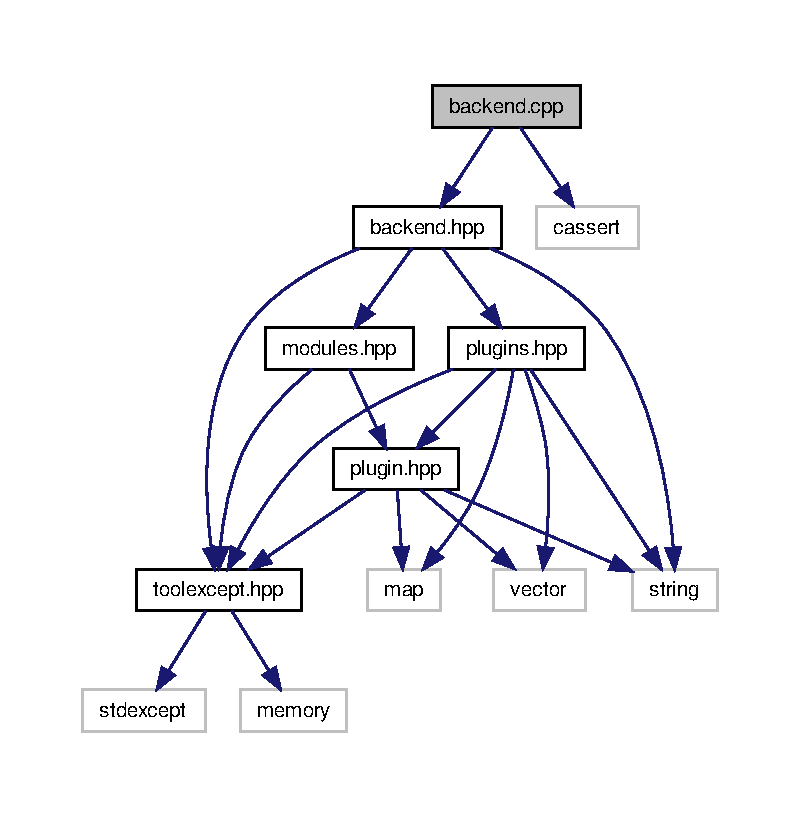
\includegraphics[width=350pt]{src_2backend_8cpp__incl}
\end{center}
\end{figure}
\subsection*{Namespaces}
\begin{DoxyCompactItemize}
\item 
 \hyperlink{namespacekdb}{kdb}
\begin{DoxyCompactList}\small\item\em This is the main namespace for the C++ binding and libraries. \end{DoxyCompactList}\item 
 \hyperlink{namespacekdb_1_1tools}{kdb\+::tools}
\begin{DoxyCompactList}\small\item\em This namespace is for the libtool library. \end{DoxyCompactList}\end{DoxyCompactItemize}
\subsection*{Functions}
\begin{DoxyCompactItemize}
\item 
std\+::ostream \& \hyperlink{namespacekdb_1_1tools_a10b59213ee542e33c7ecc481d4476a79}{kdb\+::tools\+::operator$<$$<$} (std\+::ostream \&os, Backend const \&b)
\begin{DoxyCompactList}\small\item\em Prints the current status. \end{DoxyCompactList}\end{DoxyCompactItemize}


\subsection{Detailed Description}
Implementation of backend. 

\begin{DoxyCopyright}{Copyright}
B\+S\+D License (see doc/\+C\+O\+P\+Y\+I\+N\+G or \href{http://www.libelektra.org}{\tt http\+://www.\+libelektra.\+org}) 
\end{DoxyCopyright}

\hypertarget{backend_8hpp}{\section{backend.\+hpp File Reference}
\label{backend_8hpp}\index{backend.\+hpp@{backend.\+hpp}}
}


Implements a way to build and deal with a backend.  


{\ttfamily \#include $<$plugins.\+hpp$>$}\\*
{\ttfamily \#include $<$modules.\+hpp$>$}\\*
{\ttfamily \#include $<$toolexcept.\+hpp$>$}\\*
{\ttfamily \#include $<$ostream$>$}\\*
{\ttfamily \#include $<$string$>$}\\*
{\ttfamily \#include $<$kdb.\+hpp$>$}\\*
Include dependency graph for backend.\+hpp\+:
\nopagebreak
\begin{figure}[H]
\begin{center}
\leavevmode
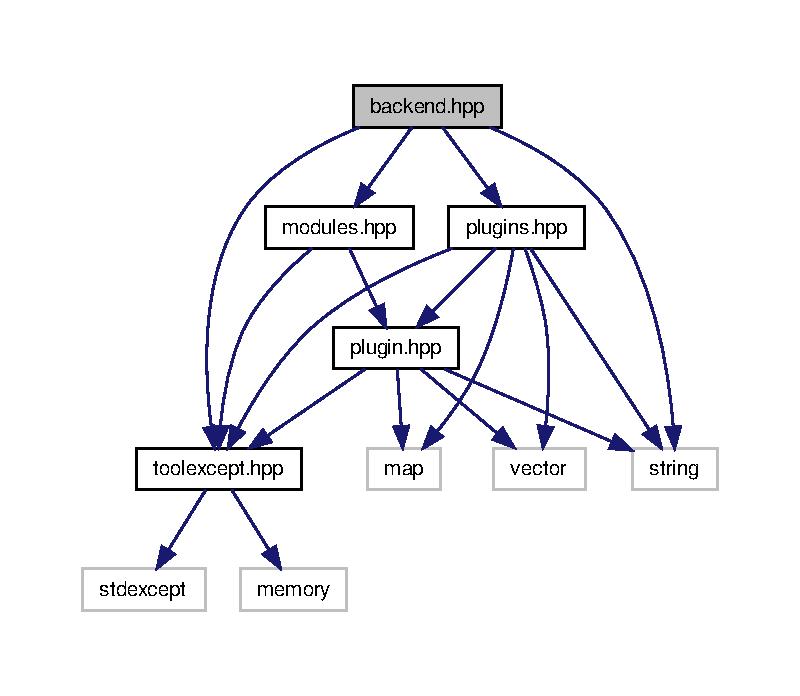
\includegraphics[width=350pt]{backend_8hpp__incl}
\end{center}
\end{figure}
This graph shows which files directly or indirectly include this file\+:
\nopagebreak
\begin{figure}[H]
\begin{center}
\leavevmode
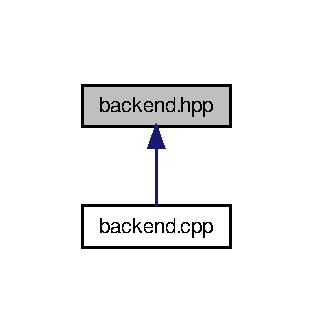
\includegraphics[width=350pt]{backend_8hpp__dep__incl}
\end{center}
\end{figure}
\subsection*{Data Structures}
\begin{DoxyCompactItemize}
\item 
class \hyperlink{classkdb_1_1tools_1_1Backend}{kdb\+::tools\+::\+Backend}
\begin{DoxyCompactList}\small\item\em A representation of the backend (= set of plugins) that can be mounted. \end{DoxyCompactList}\end{DoxyCompactItemize}
\subsection*{Namespaces}
\begin{DoxyCompactItemize}
\item 
 \hyperlink{namespacekdb}{kdb}
\begin{DoxyCompactList}\small\item\em This is the main namespace for the C++ binding and libraries. \end{DoxyCompactList}\item 
 \hyperlink{namespacekdb_1_1tools}{kdb\+::tools}
\begin{DoxyCompactList}\small\item\em This namespace is for the libtool library. \end{DoxyCompactList}\end{DoxyCompactItemize}
\subsection*{Functions}
\begin{DoxyCompactItemize}
\item 
std\+::ostream \& \hyperlink{namespacekdb_1_1tools_a10b59213ee542e33c7ecc481d4476a79}{kdb\+::tools\+::operator$<$$<$} (std\+::ostream \&os, Backend const \&b)
\begin{DoxyCompactList}\small\item\em Prints the current status. \end{DoxyCompactList}\end{DoxyCompactItemize}


\subsection{Detailed Description}
Implements a way to build and deal with a backend. 

\begin{DoxyCopyright}{Copyright}
B\+S\+D License (see doc/\+C\+O\+P\+Y\+I\+N\+G or \href{http://www.libelektra.org}{\tt http\+://www.\+libelektra.\+org}) 
\end{DoxyCopyright}

\hypertarget{backends_8hpp}{}\section{backends.\+hpp File Reference}
\label{backends_8hpp}\index{backends.\+hpp@{backends.\+hpp}}


Allows one to list all available backends.  


{\ttfamily \#include $<$string$>$}\newline
{\ttfamily \#include $<$vector$>$}\newline
{\ttfamily \#include $<$keyset.\+hpp$>$}\newline
{\ttfamily \#include $<$toolexcept.\+hpp$>$}\newline
Include dependency graph for backends.\+hpp\+:
\nopagebreak
\begin{figure}[H]
\begin{center}
\leavevmode
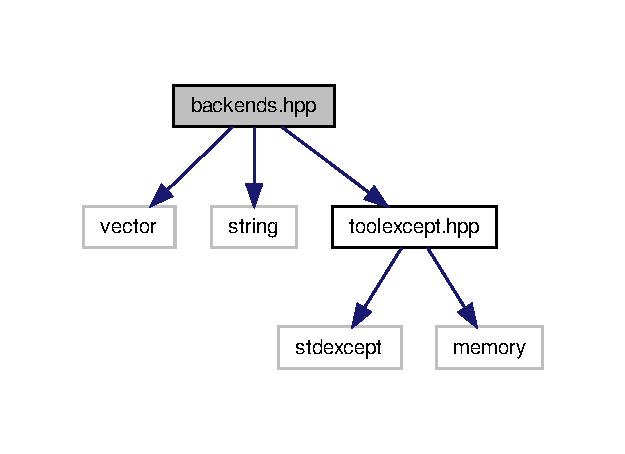
\includegraphics[width=350pt]{backends_8hpp__incl}
\end{center}
\end{figure}
This graph shows which files directly or indirectly include this file\+:
\nopagebreak
\begin{figure}[H]
\begin{center}
\leavevmode
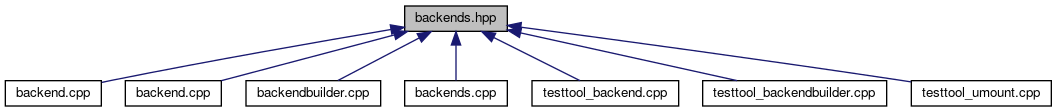
\includegraphics[width=350pt]{backends_8hpp__dep__incl}
\end{center}
\end{figure}
\subsection*{Classes}
\begin{DoxyCompactItemize}
\item 
struct \hyperlink{structkdb_1_1tools_1_1BackendInfo}{kdb\+::tools\+::\+Backend\+Info}
\begin{DoxyCompactList}\small\item\em Info about a backend. \end{DoxyCompactList}\item 
class \hyperlink{classkdb_1_1tools_1_1Backends}{kdb\+::tools\+::\+Backends}
\begin{DoxyCompactList}\small\item\em Allows one to list backends. \end{DoxyCompactList}\end{DoxyCompactItemize}
\subsection*{Namespaces}
\begin{DoxyCompactItemize}
\item 
 \hyperlink{namespacekdb}{kdb}
\begin{DoxyCompactList}\small\item\em This is the main namespace for the C++ binding and libraries. \end{DoxyCompactList}\item 
 \hyperlink{namespacekdb_1_1tools}{kdb\+::tools}
\begin{DoxyCompactList}\small\item\em This namespace is for the libtool library. \end{DoxyCompactList}\end{DoxyCompactItemize}


\subsection{Detailed Description}
Allows one to list all available backends. 

\begin{DoxyCopyright}{Copyright}
B\+SD License (see L\+I\+C\+E\+N\+S\+E.\+md or \href{https://www.libelektra.org}{\tt https\+://www.\+libelektra.\+org}) 
\end{DoxyCopyright}

\hypertarget{modules_8cpp}{}\section{modules.\+cpp File Reference}
\label{modules_8cpp}\index{modules.\+cpp@{modules.\+cpp}}


Implementation of module loading.  


{\ttfamily \#include $<$keyset.\+hpp$>$}\newline
{\ttfamily \#include $<$modules.\+hpp$>$}\newline
{\ttfamily \#include $<$kdbmodule.\+h$>$}\newline
{\ttfamily \#include $<$kdbplugin.\+h$>$}\newline
Include dependency graph for modules.\+cpp\+:
\nopagebreak
\begin{figure}[H]
\begin{center}
\leavevmode
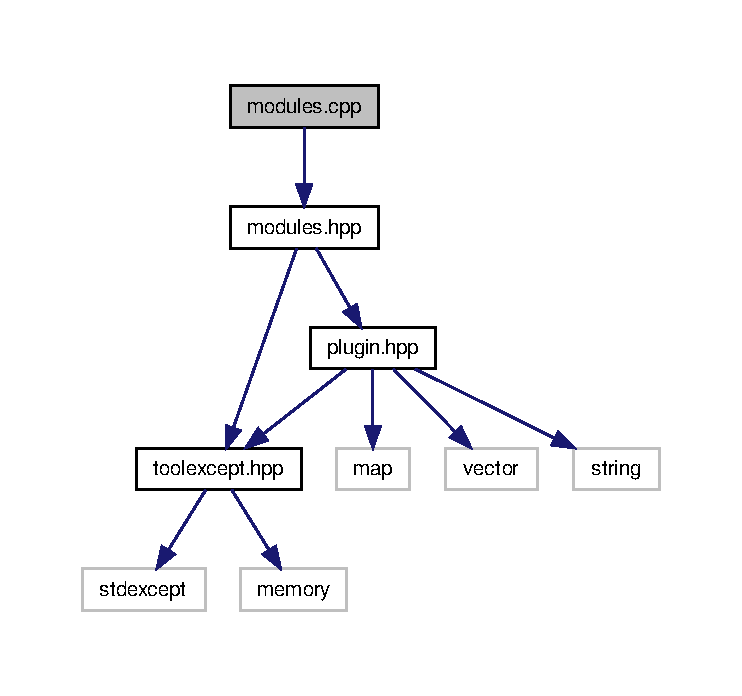
\includegraphics[width=350pt]{modules_8cpp__incl}
\end{center}
\end{figure}
\subsection*{Namespaces}
\begin{DoxyCompactItemize}
\item 
 \hyperlink{namespacekdb}{kdb}
\begin{DoxyCompactList}\small\item\em This is the main namespace for the C++ binding and libraries. \end{DoxyCompactList}\item 
 \hyperlink{namespacekdb_1_1tools}{kdb\+::tools}
\begin{DoxyCompactList}\small\item\em This namespace is for the libtool library. \end{DoxyCompactList}\end{DoxyCompactItemize}


\subsection{Detailed Description}
Implementation of module loading. 

\begin{DoxyCopyright}{Copyright}
B\+SD License (see L\+I\+C\+E\+N\+S\+E.\+md or \href{https://www.libelektra.org}{\tt https\+://www.\+libelektra.\+org}) 
\end{DoxyCopyright}

\hypertarget{modules_8hpp}{\section{modules.\+hpp File Reference}
\label{modules_8hpp}\index{modules.\+hpp@{modules.\+hpp}}
}


Allows one to load plugins.  


{\ttfamily \#include $<$plugin.\+hpp$>$}\\*
{\ttfamily \#include $<$keyset.\+hpp$>$}\\*
{\ttfamily \#include $<$toolexcept.\+hpp$>$}\\*
Include dependency graph for modules.\+hpp\+:
\nopagebreak
\begin{figure}[H]
\begin{center}
\leavevmode
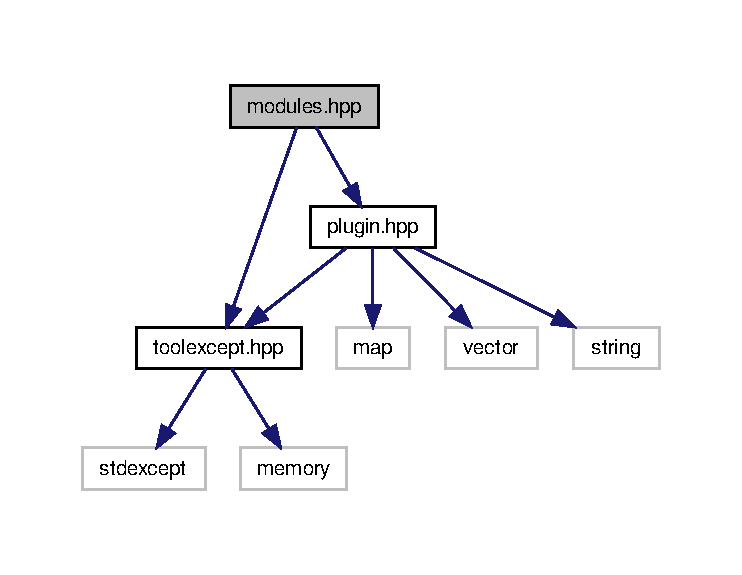
\includegraphics[width=350pt]{modules_8hpp__incl}
\end{center}
\end{figure}
This graph shows which files directly or indirectly include this file\+:
\nopagebreak
\begin{figure}[H]
\begin{center}
\leavevmode
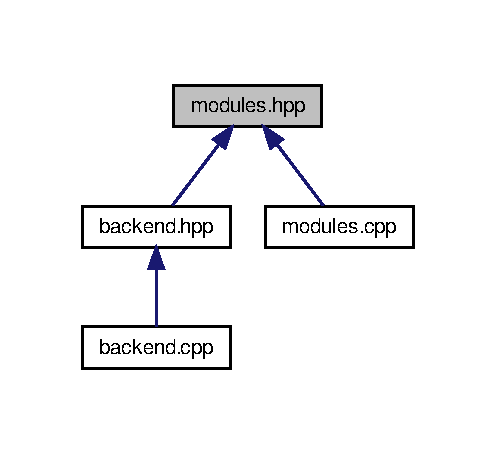
\includegraphics[width=350pt]{modules_8hpp__dep__incl}
\end{center}
\end{figure}
\subsection*{Data Structures}
\begin{DoxyCompactItemize}
\item 
class \hyperlink{classkdb_1_1tools_1_1Modules}{kdb\+::tools\+::\+Modules}
\begin{DoxyCompactList}\small\item\em Allows one to load plugins. \end{DoxyCompactList}\end{DoxyCompactItemize}
\subsection*{Namespaces}
\begin{DoxyCompactItemize}
\item 
 \hyperlink{namespacekdb}{kdb}
\begin{DoxyCompactList}\small\item\em This is the main namespace for the C++ binding and libraries. \end{DoxyCompactList}\item 
 \hyperlink{namespacekdb_1_1tools}{kdb\+::tools}
\begin{DoxyCompactList}\small\item\em This namespace is for the libtool library. \end{DoxyCompactList}\end{DoxyCompactItemize}


\subsection{Detailed Description}
Allows one to load plugins. 

\begin{DoxyCopyright}{Copyright}
B\+S\+D License (see doc/\+C\+O\+P\+Y\+I\+N\+G or \href{http://www.libelektra.org}{\tt http\+://www.\+libelektra.\+org}) 
\end{DoxyCopyright}

\hypertarget{plugin_8cpp}{}\doxysection{plugin.\+cpp File Reference}
\label{plugin_8cpp}\index{plugin.cpp@{plugin.cpp}}


Implementation of plugin.  


{\ttfamily \#include $<$kdb.\+hpp$>$}\newline
{\ttfamily \#include $<$helper/keyhelper.\+hpp$>$}\newline
{\ttfamily \#include $<$kdb.\+h$>$}\newline
{\ttfamily \#include $<$kdbmodule.\+h$>$}\newline
{\ttfamily \#include $<$kdbplugin.\+h$>$}\newline
{\ttfamily \#include $<$kdbprivate.\+h$>$}\newline
{\ttfamily \#include $<$plugindatabase.\+hpp$>$}\newline
{\ttfamily \#include $<$algorithm$>$}\newline
{\ttfamily \#include $<$set$>$}\newline
{\ttfamily \#include $<$plugin.\+hpp$>$}\newline
{\ttfamily \#include $<$stdio.\+h$>$}\newline
Include dependency graph for plugin.\+cpp\+:
\nopagebreak
\begin{figure}[H]
\begin{center}
\leavevmode
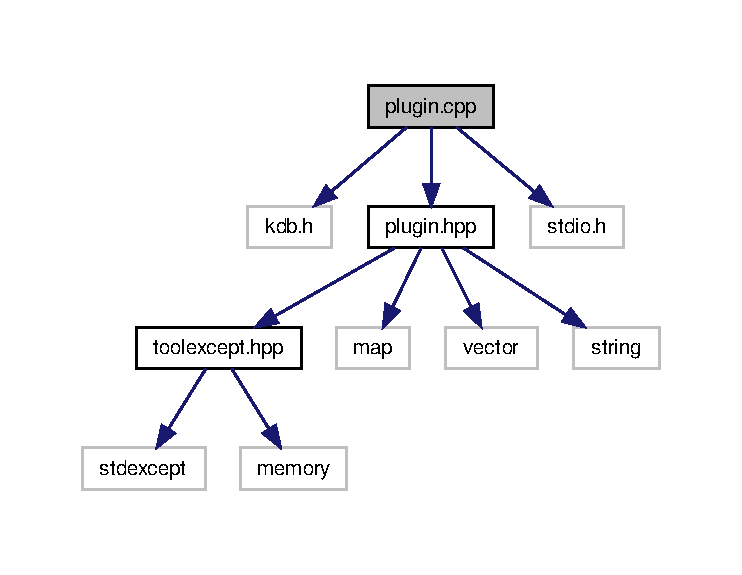
\includegraphics[width=350pt]{plugin_8cpp__incl}
\end{center}
\end{figure}
\doxysubsection*{Namespaces}
\begin{DoxyCompactItemize}
\item 
 \mbox{\hyperlink{namespacekdb}{kdb}}
\begin{DoxyCompactList}\small\item\em This is the main namespace for the C++ binding and libraries. \end{DoxyCompactList}\item 
 \mbox{\hyperlink{namespacekdb_1_1tools}{kdb\+::tools}}
\begin{DoxyCompactList}\small\item\em This namespace is for the libtool library. \end{DoxyCompactList}\end{DoxyCompactItemize}


\doxysubsection{Detailed Description}
Implementation of plugin. 

\begin{DoxyCopyright}{Copyright}
B\+SD License (see L\+I\+C\+E\+N\+S\+E.\+md or \href{https://www.libelektra.org}{\texttt{ https\+://www.\+libelektra.\+org}}) 
\end{DoxyCopyright}

\hypertarget{plugin_8hpp}{\section{plugin.\+hpp File Reference}
\label{plugin_8hpp}\index{plugin.\+hpp@{plugin.\+hpp}}
}


Header file of plugin.  


{\ttfamily \#include $<$kdb.\+hpp$>$}\\*
{\ttfamily \#include $<$pluginspec.\+hpp$>$}\\*
{\ttfamily \#include $<$toolexcept.\+hpp$>$}\\*
{\ttfamily \#include $<$map$>$}\\*
{\ttfamily \#include $<$string$>$}\\*
{\ttfamily \#include $<$vector$>$}\\*
Include dependency graph for plugin.\+hpp\+:
\nopagebreak
\begin{figure}[H]
\begin{center}
\leavevmode
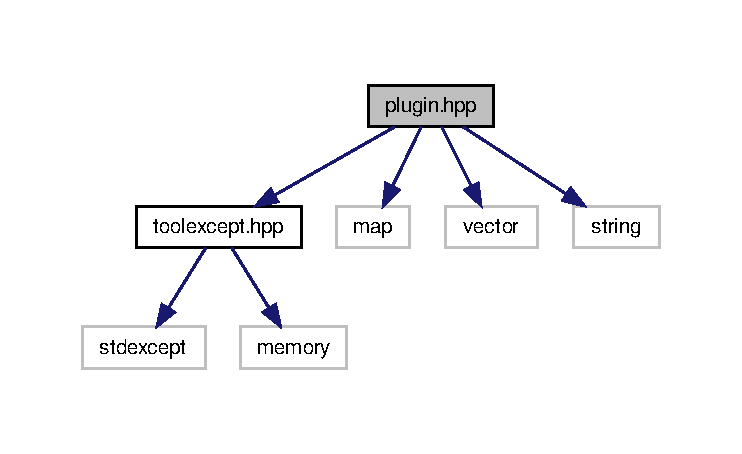
\includegraphics[width=350pt]{plugin_8hpp__incl}
\end{center}
\end{figure}
This graph shows which files directly or indirectly include this file\+:
\nopagebreak
\begin{figure}[H]
\begin{center}
\leavevmode
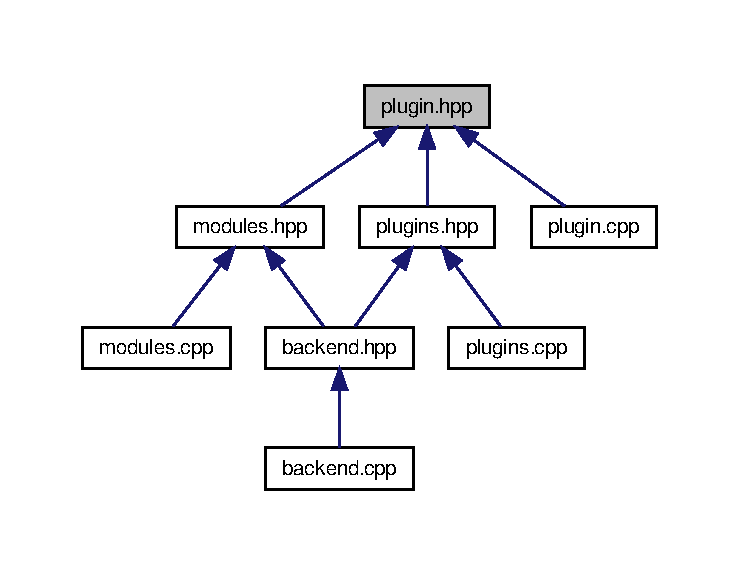
\includegraphics[width=350pt]{plugin_8hpp__dep__incl}
\end{center}
\end{figure}
\subsection*{Data Structures}
\begin{DoxyCompactItemize}
\item 
class \hyperlink{classkdb_1_1tools_1_1Plugin}{kdb\+::tools\+::\+Plugin}
\begin{DoxyCompactList}\small\item\em This is a C++ representation of a plugin. \end{DoxyCompactList}\end{DoxyCompactItemize}
\subsection*{Namespaces}
\begin{DoxyCompactItemize}
\item 
 \hyperlink{namespacekdb}{kdb}
\begin{DoxyCompactList}\small\item\em This is the main namespace for the C++ binding and libraries. \end{DoxyCompactList}\item 
 \hyperlink{namespacekdb_1_1tools}{kdb\+::tools}
\begin{DoxyCompactList}\small\item\em This namespace is for the libtool library. \end{DoxyCompactList}\end{DoxyCompactItemize}


\subsection{Detailed Description}
Header file of plugin. 

\begin{DoxyCopyright}{Copyright}
B\+S\+D License (see doc/\+C\+O\+P\+Y\+I\+N\+G or \href{http://www.libelektra.org}{\tt http\+://www.\+libelektra.\+org}) 
\end{DoxyCopyright}

\hypertarget{plugins_8cpp}{\section{plugins.\+cpp File Reference}
\label{plugins_8cpp}\index{plugins.\+cpp@{plugins.\+cpp}}
}


Implementation of set/get/error plugins.  


{\ttfamily \#include $<$helper/keyhelper.\+hpp$>$}\\*
{\ttfamily \#include $<$plugins.\+hpp$>$}\\*
{\ttfamily \#include $<$kdbprivate.\+h$>$}\\*
{\ttfamily \#include $<$algorithm$>$}\\*
{\ttfamily \#include $<$iterator$>$}\\*
Include dependency graph for plugins.\+cpp\+:
\nopagebreak
\begin{figure}[H]
\begin{center}
\leavevmode
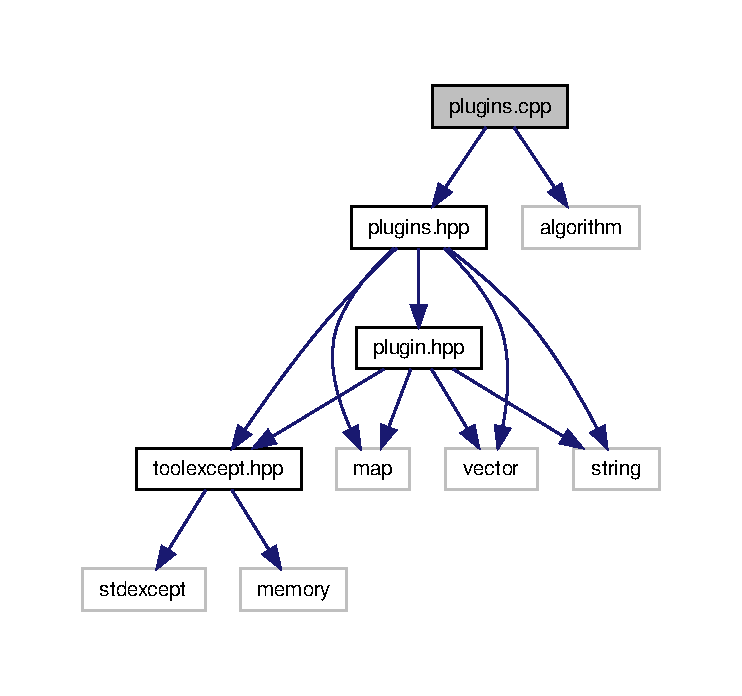
\includegraphics[width=350pt]{plugins_8cpp__incl}
\end{center}
\end{figure}
\subsection*{Namespaces}
\begin{DoxyCompactItemize}
\item 
 \hyperlink{namespacekdb}{kdb}
\begin{DoxyCompactList}\small\item\em This is the main namespace for the C++ binding and libraries. \end{DoxyCompactList}\item 
 \hyperlink{namespacekdb_1_1tools}{kdb\+::tools}
\begin{DoxyCompactList}\small\item\em This namespace is for the libtool library. \end{DoxyCompactList}\end{DoxyCompactItemize}


\subsection{Detailed Description}
Implementation of set/get/error plugins. 

\begin{DoxyCopyright}{Copyright}
B\+S\+D License (see doc/\+L\+I\+C\+E\+N\+S\+E.\+md or \href{http://www.libelektra.org}{\tt http\+://www.\+libelektra.\+org}) 
\end{DoxyCopyright}

\hypertarget{plugins_8hpp}{}\doxysection{plugins.\+hpp File Reference}
\label{plugins_8hpp}\index{plugins.hpp@{plugins.hpp}}


Implementation of get/set and error plugins.  


{\ttfamily \#include $<$plugin.\+hpp$>$}\newline
{\ttfamily \#include $<$toolexcept.\+hpp$>$}\newline
{\ttfamily \#include $<$map$>$}\newline
{\ttfamily \#include $<$string$>$}\newline
{\ttfamily \#include $<$vector$>$}\newline
{\ttfamily \#include $<$kdb.\+hpp$>$}\newline
Include dependency graph for plugins.\+hpp\+:
\nopagebreak
\begin{figure}[H]
\begin{center}
\leavevmode
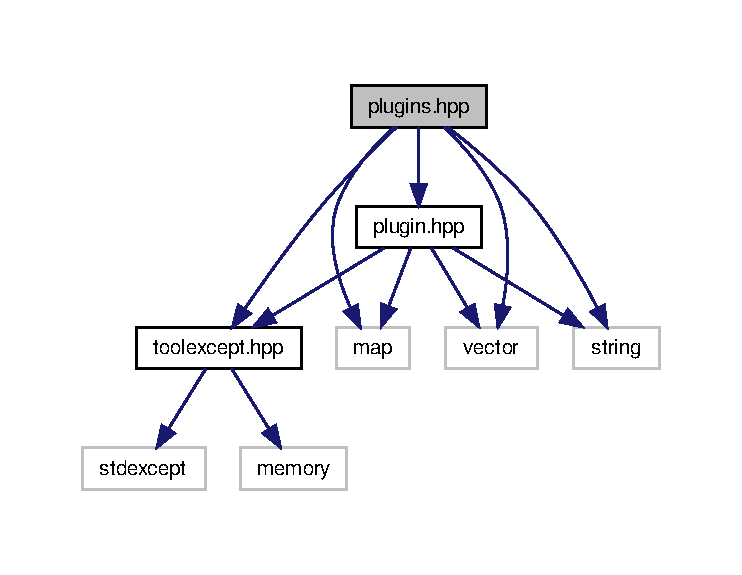
\includegraphics[width=350pt]{plugins_8hpp__incl}
\end{center}
\end{figure}
This graph shows which files directly or indirectly include this file\+:
\nopagebreak
\begin{figure}[H]
\begin{center}
\leavevmode
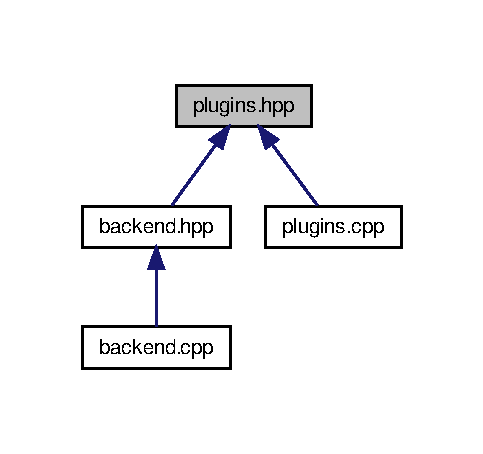
\includegraphics[width=350pt]{plugins_8hpp__dep__incl}
\end{center}
\end{figure}
\doxysubsection*{Classes}
\begin{DoxyCompactItemize}
\item 
class \mbox{\hyperlink{classkdb_1_1tools_1_1Plugins}{kdb\+::tools\+::\+Plugins}}
\begin{DoxyCompactList}\small\item\em A collection of plugins (either get, set or error) \end{DoxyCompactList}\item 
class \mbox{\hyperlink{classkdb_1_1tools_1_1GetPlugins}{kdb\+::tools\+::\+Get\+Plugins}}
\begin{DoxyCompactList}\small\item\em \mbox{\hyperlink{classkdb_1_1tools_1_1Plugins}{Plugins}} to get configuration. \end{DoxyCompactList}\item 
class \mbox{\hyperlink{classkdb_1_1tools_1_1SetPlugins}{kdb\+::tools\+::\+Set\+Plugins}}
\begin{DoxyCompactList}\small\item\em \mbox{\hyperlink{classkdb_1_1tools_1_1Plugins}{Plugins}} to set configuration. \end{DoxyCompactList}\item 
class \mbox{\hyperlink{classkdb_1_1tools_1_1ErrorPlugins}{kdb\+::tools\+::\+Error\+Plugins}}
\begin{DoxyCompactList}\small\item\em \mbox{\hyperlink{classkdb_1_1tools_1_1Plugins}{Plugins}} to handle errors during configuration access. \end{DoxyCompactList}\item 
class \mbox{\hyperlink{classkdb_1_1tools_1_1CommitPlugins}{kdb\+::tools\+::\+Commit\+Plugins}}
\begin{DoxyCompactList}\small\item\em \mbox{\hyperlink{classkdb_1_1tools_1_1Plugins}{Plugins}} to handle errors during configuration access. \end{DoxyCompactList}\end{DoxyCompactItemize}
\doxysubsection*{Namespaces}
\begin{DoxyCompactItemize}
\item 
 \mbox{\hyperlink{namespacekdb}{kdb}}
\begin{DoxyCompactList}\small\item\em This is the main namespace for the C++ binding and libraries. \end{DoxyCompactList}\item 
 \mbox{\hyperlink{namespacekdb_1_1tools}{kdb\+::tools}}
\begin{DoxyCompactList}\small\item\em This namespace is for the libtool library. \end{DoxyCompactList}\end{DoxyCompactItemize}


\doxysubsection{Detailed Description}
Implementation of get/set and error plugins. 

\begin{DoxyCopyright}{Copyright}
BSD License (see LICENSE.\+md or \href{https://www.libelektra.org}{\texttt{ https\+://www.\+libelektra.\+org}}) 
\end{DoxyCopyright}

\hypertarget{toolexcept_8hpp}{\section{toolexcept.\+hpp File Reference}
\label{toolexcept_8hpp}\index{toolexcept.\+hpp@{toolexcept.\+hpp}}
}


Implementation of all exceptions elektratools library might throw.  


{\ttfamily \#include $<$memory$>$}\\*
{\ttfamily \#include $<$stdexcept$>$}\\*
{\ttfamily \#include $<$kdbio.\+hpp$>$}\\*
Include dependency graph for toolexcept.\+hpp\+:
\nopagebreak
\begin{figure}[H]
\begin{center}
\leavevmode
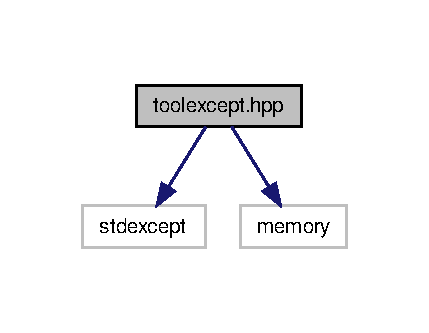
\includegraphics[width=350pt]{toolexcept_8hpp__incl}
\end{center}
\end{figure}
This graph shows which files directly or indirectly include this file\+:
\nopagebreak
\begin{figure}[H]
\begin{center}
\leavevmode
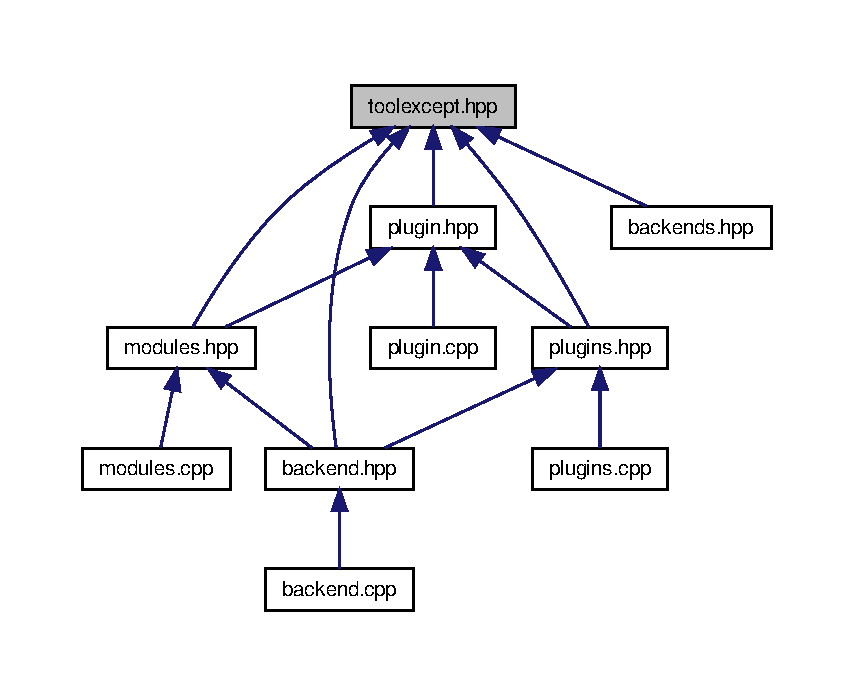
\includegraphics[width=350pt]{toolexcept_8hpp__dep__incl}
\end{center}
\end{figure}
\subsection*{Data Structures}
\begin{DoxyCompactItemize}
\item 
struct \hyperlink{structkdb_1_1tools_1_1ToolException}{kdb\+::tools\+::\+Tool\+Exception}
\begin{DoxyCompactList}\small\item\em All exceptions from the elektratools library are derived from this exception. \end{DoxyCompactList}\end{DoxyCompactItemize}
\subsection*{Namespaces}
\begin{DoxyCompactItemize}
\item 
 \hyperlink{namespacekdb}{kdb}
\begin{DoxyCompactList}\small\item\em This is the main namespace for the C++ binding and libraries. \end{DoxyCompactList}\item 
 \hyperlink{namespacekdb_1_1tools}{kdb\+::tools}
\begin{DoxyCompactList}\small\item\em This namespace is for the libtool library. \end{DoxyCompactList}\end{DoxyCompactItemize}


\subsection{Detailed Description}
Implementation of all exceptions elektratools library might throw. 

\begin{DoxyCopyright}{Copyright}
B\+S\+D License (see doc/\+L\+I\+C\+E\+N\+S\+E.\+md or \href{http://www.libelektra.org}{\tt http\+://www.\+libelektra.\+org}) 
\end{DoxyCopyright}

\printindex
\end{document}
